\documentclass{article}
\usepackage[utf8]{inputenc}
\usepackage[left=1cm, right=1cm, top=2cm, bottom=2cm]{geometry}
\usepackage{graphicx}
\usepackage{caption}
\usepackage{subcaption}
\usepackage{amsmath}
\usepackage{booktabs} 
\usepackage{float}
\usepackage[colorlinks=true, urlcolor=blue, linkcolor=blue, citecolor=blue]{hyperref}
\usepackage{cleveref}

\title{Project 1}
\author{Masum Billah, Madhu Chencharapu, Gabriel Loos, Brendan McDonnell, Roshan Ravichandran}
\date{February 2026}

\begin{document}

\maketitle

\section{Introduction}

In this project, we will explore three different datasets using multiple linear regression, ridge regression, lasso regression, transformed regression (specifically Sqrt, Log1p, and Box-Cox), and second-order polynomial regression including interaction terms. The three datasets we will be using are:

\begin{itemize}
	\item \textbf{Auto MPG:} This dataset contains information about different cars. The goal is to predict the miles per gallon (MPG) given the other characteristics of the car. The dataset can be found at \url{https://archive.ics.uci.edu/dataset}.
	\item \textbf{California Housing Prices:} This dataset contains information about different housing locations. The goal is to predict the median house price of the area given the other characteristics. The dataset can be found at \url{https://www.kaggle.com/datasets/camnugent/california-housing-prices}.
	\item \textbf{Insurance Charges:} This dataset contains information about different primary beneficiaries of health insurance. The goal is to predict the primary beneficiaries insurance charges given their other characteristics. The dataset can be found at \url{https://www.kaggle.com/datasets/mirichoi0218/insurance}.
\end{itemize}

\section{Summary of Methods and Key Results}

\subsection{Methods Overview}

On each dataset, we will test the performance of multiple linear regression, ridge regression, lasso regression, Sqrt transformed regression, Log1p transformed regression, Box-Cox transformed regression, and second-order polynomial regression including interaction terms. Each model was evaluated using In-Sample, Out-of-Sample (80-20 split), and Cross Validation. Additionally, we employed forward, backward, and stepwise selection procedures across all the models.

To optimize the regularization hyperparameter for Ridge and Lasso regression, we employed a three-stage grid search, using 5-fold cross-validation to maximize the mean $R^2$ score.
\begin{itemize}
	\item Stage 1: A broad logarithmic search to find the general neighborhood of the best hyperparameter.
	\item Stage 2: An intermediate refinement around the Stage 1 winner.
	\item Stage 3: A high-resolution linear search to finalize the value based on the Stage 2 results.
\end{itemize}
For the second-order polynomial regression model, we used ridge regression to prevent overfitting. To optimize the power transformation lambda for Box-Cox, we employed a grid search of standard power transformations to determine which lambda yields the highest mean $R^2$ via 5-fold cross-validation.

\subsection{Key Results}

\subsubsection{Auto MPG}

The Auto MPG dataset exhibited several non-linear trends between vehicle attributes (such as weight and horsepower) and mpg. Consequently, the second-order polynomial regression model yielded the most accurate predictions, slightly outperforming the Box-Cox Transformed model. The polynomial model utilized $\ell_2$ regularization to prevent overfitting, while the Box-Cox model applied a $\lambda = -0.5$ transformation across both platforms. \Cref{tab:Auto MPG Best Model Performance Comparison} summarizes the results.

\begin{table}[H]
\centering
\caption{Auto MPG Best Model Performance Comparison}
\label{tab:Auto MPG Best Model Performance Comparison}
\begin{tabular}{@{}llcc@{}}
\toprule
\textbf{Model} & \textbf{Platform} & \textbf{Hyperparameter} & \textbf{CV Average $R^2$} \\ \midrule
\textbf{Polynomial (Order 2)} & Scalation   & $\ell_2 = 2.5 \times 10^{-6}$ & $0.865$ \\
                              & Statsmodels & $\ell_2 = 1.5 \times 10^{-4}$ & $0.869$ \\ \addlinespace
\textbf{Box-Cox}              & Scalation   & $\lambda = -0.5$              & $0.856$ \\
                              & Statsmodels & $\lambda = -0.5$              & $0.853$ \\ \bottomrule
\end{tabular}
\end{table}

The following features were identified as the primary drivers of model accuracy:
\begin{itemize}
	\item \textbf{Core Attributes}: weight, horsepower, model year, and origin
	\item \textbf{Non-linear Terms}: model year $\times$ model year, weight $\times$ weight, acceleration $\times$ acceleration
	\item \textbf{Interaction Terms}: acceleration $\times$ origin, model year $\times$ origin, horsepower $\times$ model year
\end{itemize}
Note that non-linear and interaction terms were exclusive to the second-order polynomial model.

\subsubsection{California Housing Prices}

The California Housing Prices dataset proved to be highly complex, with none of the models doing particularly well. The linear regression model and ridge regression model performed identically across both platforms, indicating that the $\ell_2$ penalty had a negligible impact on the coefficients at that scale. While these models provided the most consistent results in Scalation, the second-order polynomial model achieved the highest overall accuracy in Statsmodels, aided by $\ell_2$ regularization. \Cref{tab:California Housing Prices Best Model Performance Comparison} summarizes the results.

\begin{table}[H]
\centering
\caption{California Housing Prices Best Model Performance Comparison}
\label{tab:California Housing Prices Best Model Performance Comparison}
\begin{tabular}{@{}llcc@{}}
\toprule
\textbf{Model} & \textbf{Platform} & \textbf{Hyperparameter} & \textbf{CV Average $R^2$} \\ \midrule
\textbf{Linear} & Scalation   & $-$ & $0.645$ \\
                              & Statsmodels & $-$ & $0.645$ \\ \addlinespace
\textbf{Ridge} & Scalation   & $\ell_2 = 4.5$ & $0.645$ \\
                              & Statsmodels & $\ell_2 = 7.5 \times 10^{-4}$ & $0.645$ \\ \addlinespace
\textbf{Polynomial (Order 2)} & Scalation   & $\ell_2 = 5$ & $0.635$ \\
                              & Statsmodels & $\ell_2 = 8.5 \times 10^{-3}$ & $0.681$ \\ \bottomrule
\end{tabular}
\end{table}

The following features were identified as the primary drivers of model accuracy:
\begin{itemize}
	\item \textbf{Core Attributes}: median income, longitude, latitude, housing median age, ocean proximity
	\item \textbf{Non-linear Terms}: median income $\times$ median income, latitude $\times$ latitude
	\item \textbf{Interaction Terms}: longitude $\times$ median income, latitude $\times$ ocean proximity, housing median age $\times$ total bedrooms
\end{itemize}
Note that non-linear and interaction terms were exclusive to the second-order polynomial model.

\subsubsection{Insurance Charges}

The second-order polynomial model, aided by $\ell_2$ regularization, significantly outperformed all other models on the Insurance Charges dataset. The second best model was the Sqrt transformed model. The substantial performance gap underscores the importance of the interaction terms, particularly between BMI and smoking status, in predicting medical costs. \Cref{tab:Insurance Charges Best Model Performance Comparison} summarizes the results.

\begin{table}[H]
\centering
\caption{Insurance Charges Best Model Performance Comparison}
\label{tab:Insurance Charges Best Model Performance Comparison}
\begin{tabular}{@{}llcc@{}}
\toprule
\textbf{Model} & \textbf{Platform} & \textbf{Hyperparameter} & \textbf{CV Average $R^2$} \\ \midrule
\textbf{Polynomial (Order 2)} & Scalation   & $\ell_2 = 9.5\times10^{-3}$ & $0.834$ \\
                              & Statsmodels & $\ell_2 = 8 \times 10^{-4}$ & $0.836$ \\ \addlinespace
\textbf{Sqrt}              & Scalation   & $-$              & $0.747$ \\
                              & Statsmodels & $-$              & $0.745$ \\ \bottomrule
\end{tabular}
\end{table}

The following features were identified as the primary drivers of model accuracy:
\begin{itemize}
	\item \textbf{Core Attributes}: smoker, region, age, bmi, children
	\item \textbf{Non-linear Terms}: age $\times$ age, bmi $\times$ bmi, children $\times$ children
	\item \textbf{Interaction Terms}: bmi $\times$ smoker, children $\times$ smoker, children $\times$ sex, bmi $\times$ region
\end{itemize}
Note that non-linear and interaction terms were exclusive to the second-order polynomial model.

\subsection{Cross-Dataset Summary}

While linear models provide a solid baseline, they consistently fall short when feature interactions or quadratic relationships are present. The Second-Order Polynomial model proved to be the most versatile across the board, particularly in the Insurance and Auto MPG datasets, where the relationships between variables are driven by interaction effects rather than simple additive properties. In the more volatile California Housing dataset, the plateau in performance across all models suggests that the complexity may stem from external factors that the second-order interactions cannot fully capture. However, the consistent use of $\ell_2$ regularization (Ridge) across all three tasks was essential in keeping these high-dimensional polynomial models stable and preventing them from overfitting to noise.

The remaining three sections will give in depth analysis and metrics from each dataset: \Cref{Auto MPG} will cover the Auto MPG dataset, \Cref{House Prices} the California Housing Prices dataset, and \Cref{Insurance Charges} the Insurance Charges dataset. Each of these sections begins with an Exploratory Data Analysis (EDA), followed by the evaluations of all modeling methods.

\section{Auto MPG}\label{Auto MPG}

\subsection{Exploratory Data Analysis}

The Auto MPG dataset contains $398$ observations each having $8$ variables. These variables are:
\begin{itemize}
	\item displacement: The total volume of all the cylinders in the cars engine.
	\item cylinders: The number of cylinders the cars engine has.
	\item horsepower: The horsepower of the cars engine.
	\item weight: The weight of the car.
	\item acceleration: The time it takes the car to accelerate from $0$ mph to $60$ mph.
	\item model year: The model year of the car.
	\item origin: Where the car was manufactured. (1=USA, 2=Europe, 3=Japan)
	\item mpg: (The target variable) The miles per gallon of the car.
\end{itemize}

The horsepower feature contains six missing values, representing approximately $1.5\%$ of the dataset. Because all other features are fully populated, these rows were excluded from the analysis. For modeling purposes, we appended an intercept column of ones and converted the categorical origin variable into dummy variables (origin\_2 and origin\_3), omitting origin\_1 to prevent multi-collinearity.

Univariate distributions are visualized in \Cref{fig:Auto MPG Histograms} (histograms/count-plots) and \Cref{fig:Auto MPG Box Plots} (box plots for continuous variables). The visualizations reveal that displacement, horsepower, weight, and mpg are all right-skewed to varying degrees, whereas acceleration follows a roughly normal distribution. Notably, horsepower and acceleration both exhibit several outliers. Regarding the categorical features, the model year is distributed fairly uniformly. The majority of vehicles feature 4-cylinder engines, with 6- and 8-cylinder variants making up the remainder of the primary fleet. Finally, Origin 1 (USA) is the most prevalent, while Origin 2 (Europe) and Origin 3 (Japan) show similar levels of representation.

\begin{figure}[H]
    \centering
    \captionsetup{justification=centering}
    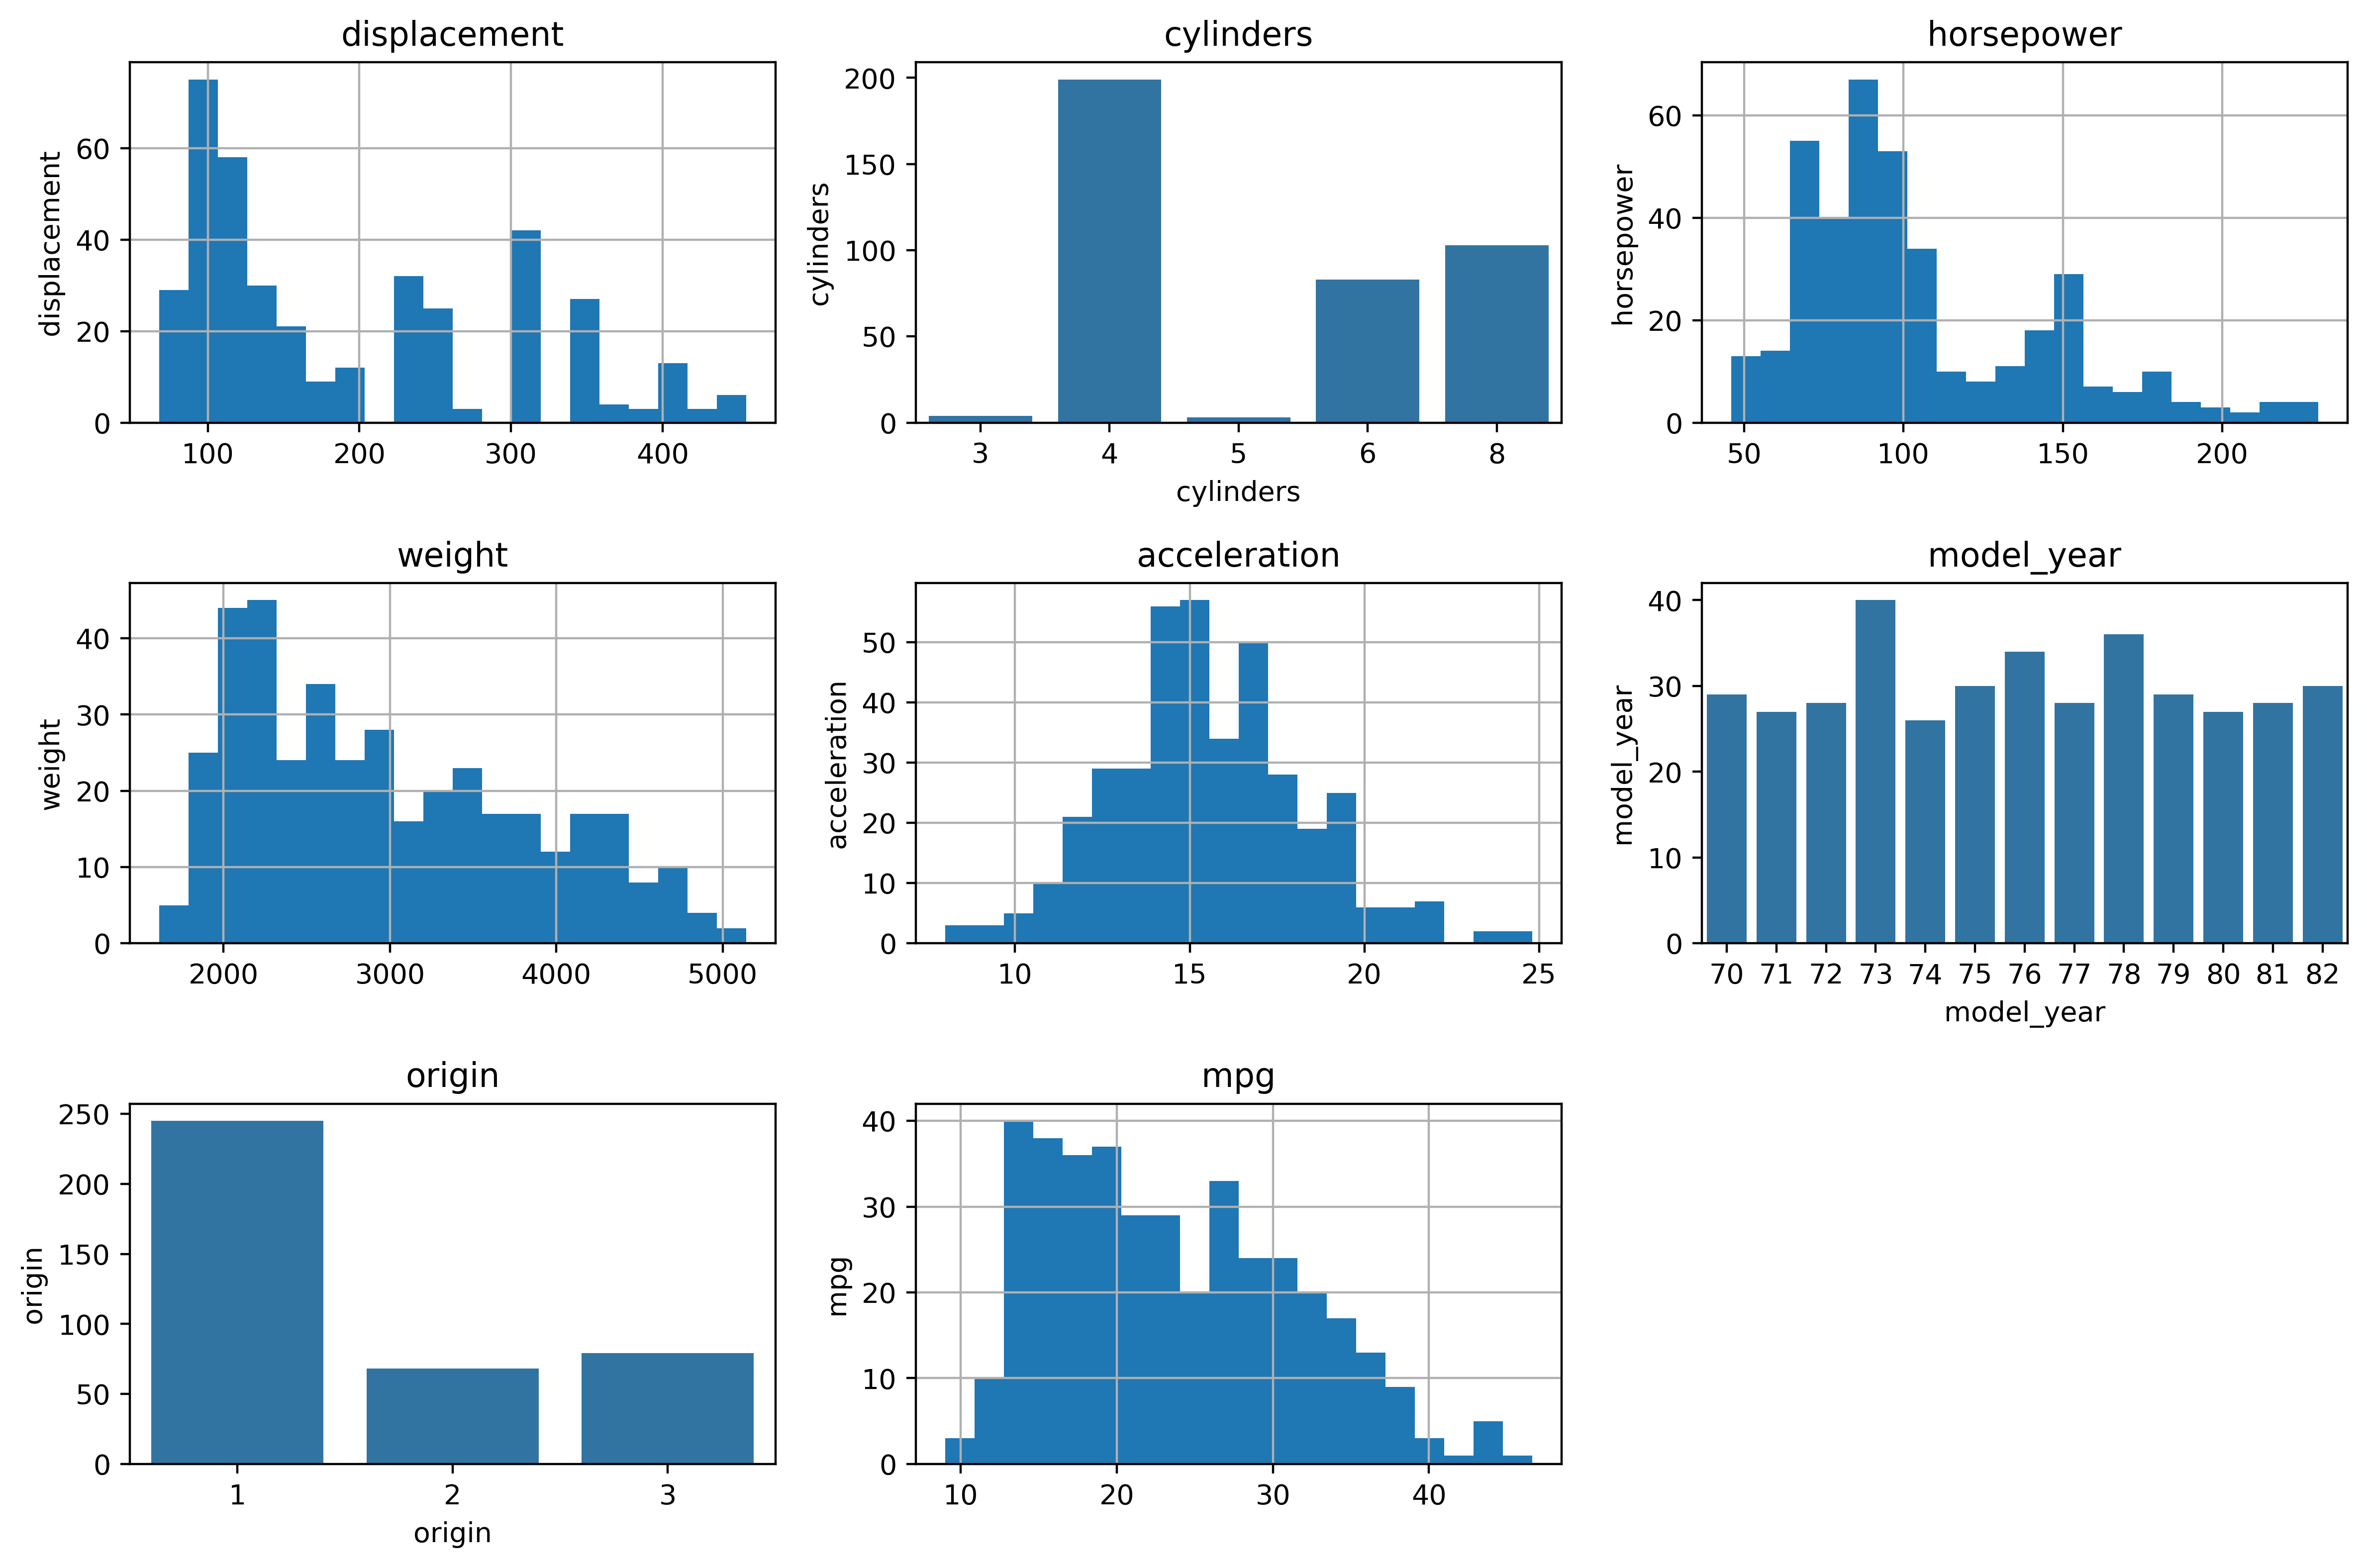
\includegraphics[width=0.75\textwidth]{../Auto_MPG/histograms.png} 
    \caption{Auto MPG Histograms and Count-Plots}
    \label{fig:Auto MPG Histograms}
\end{figure}

\begin{figure}[H]
    \centering
    \captionsetup{justification=centering}
    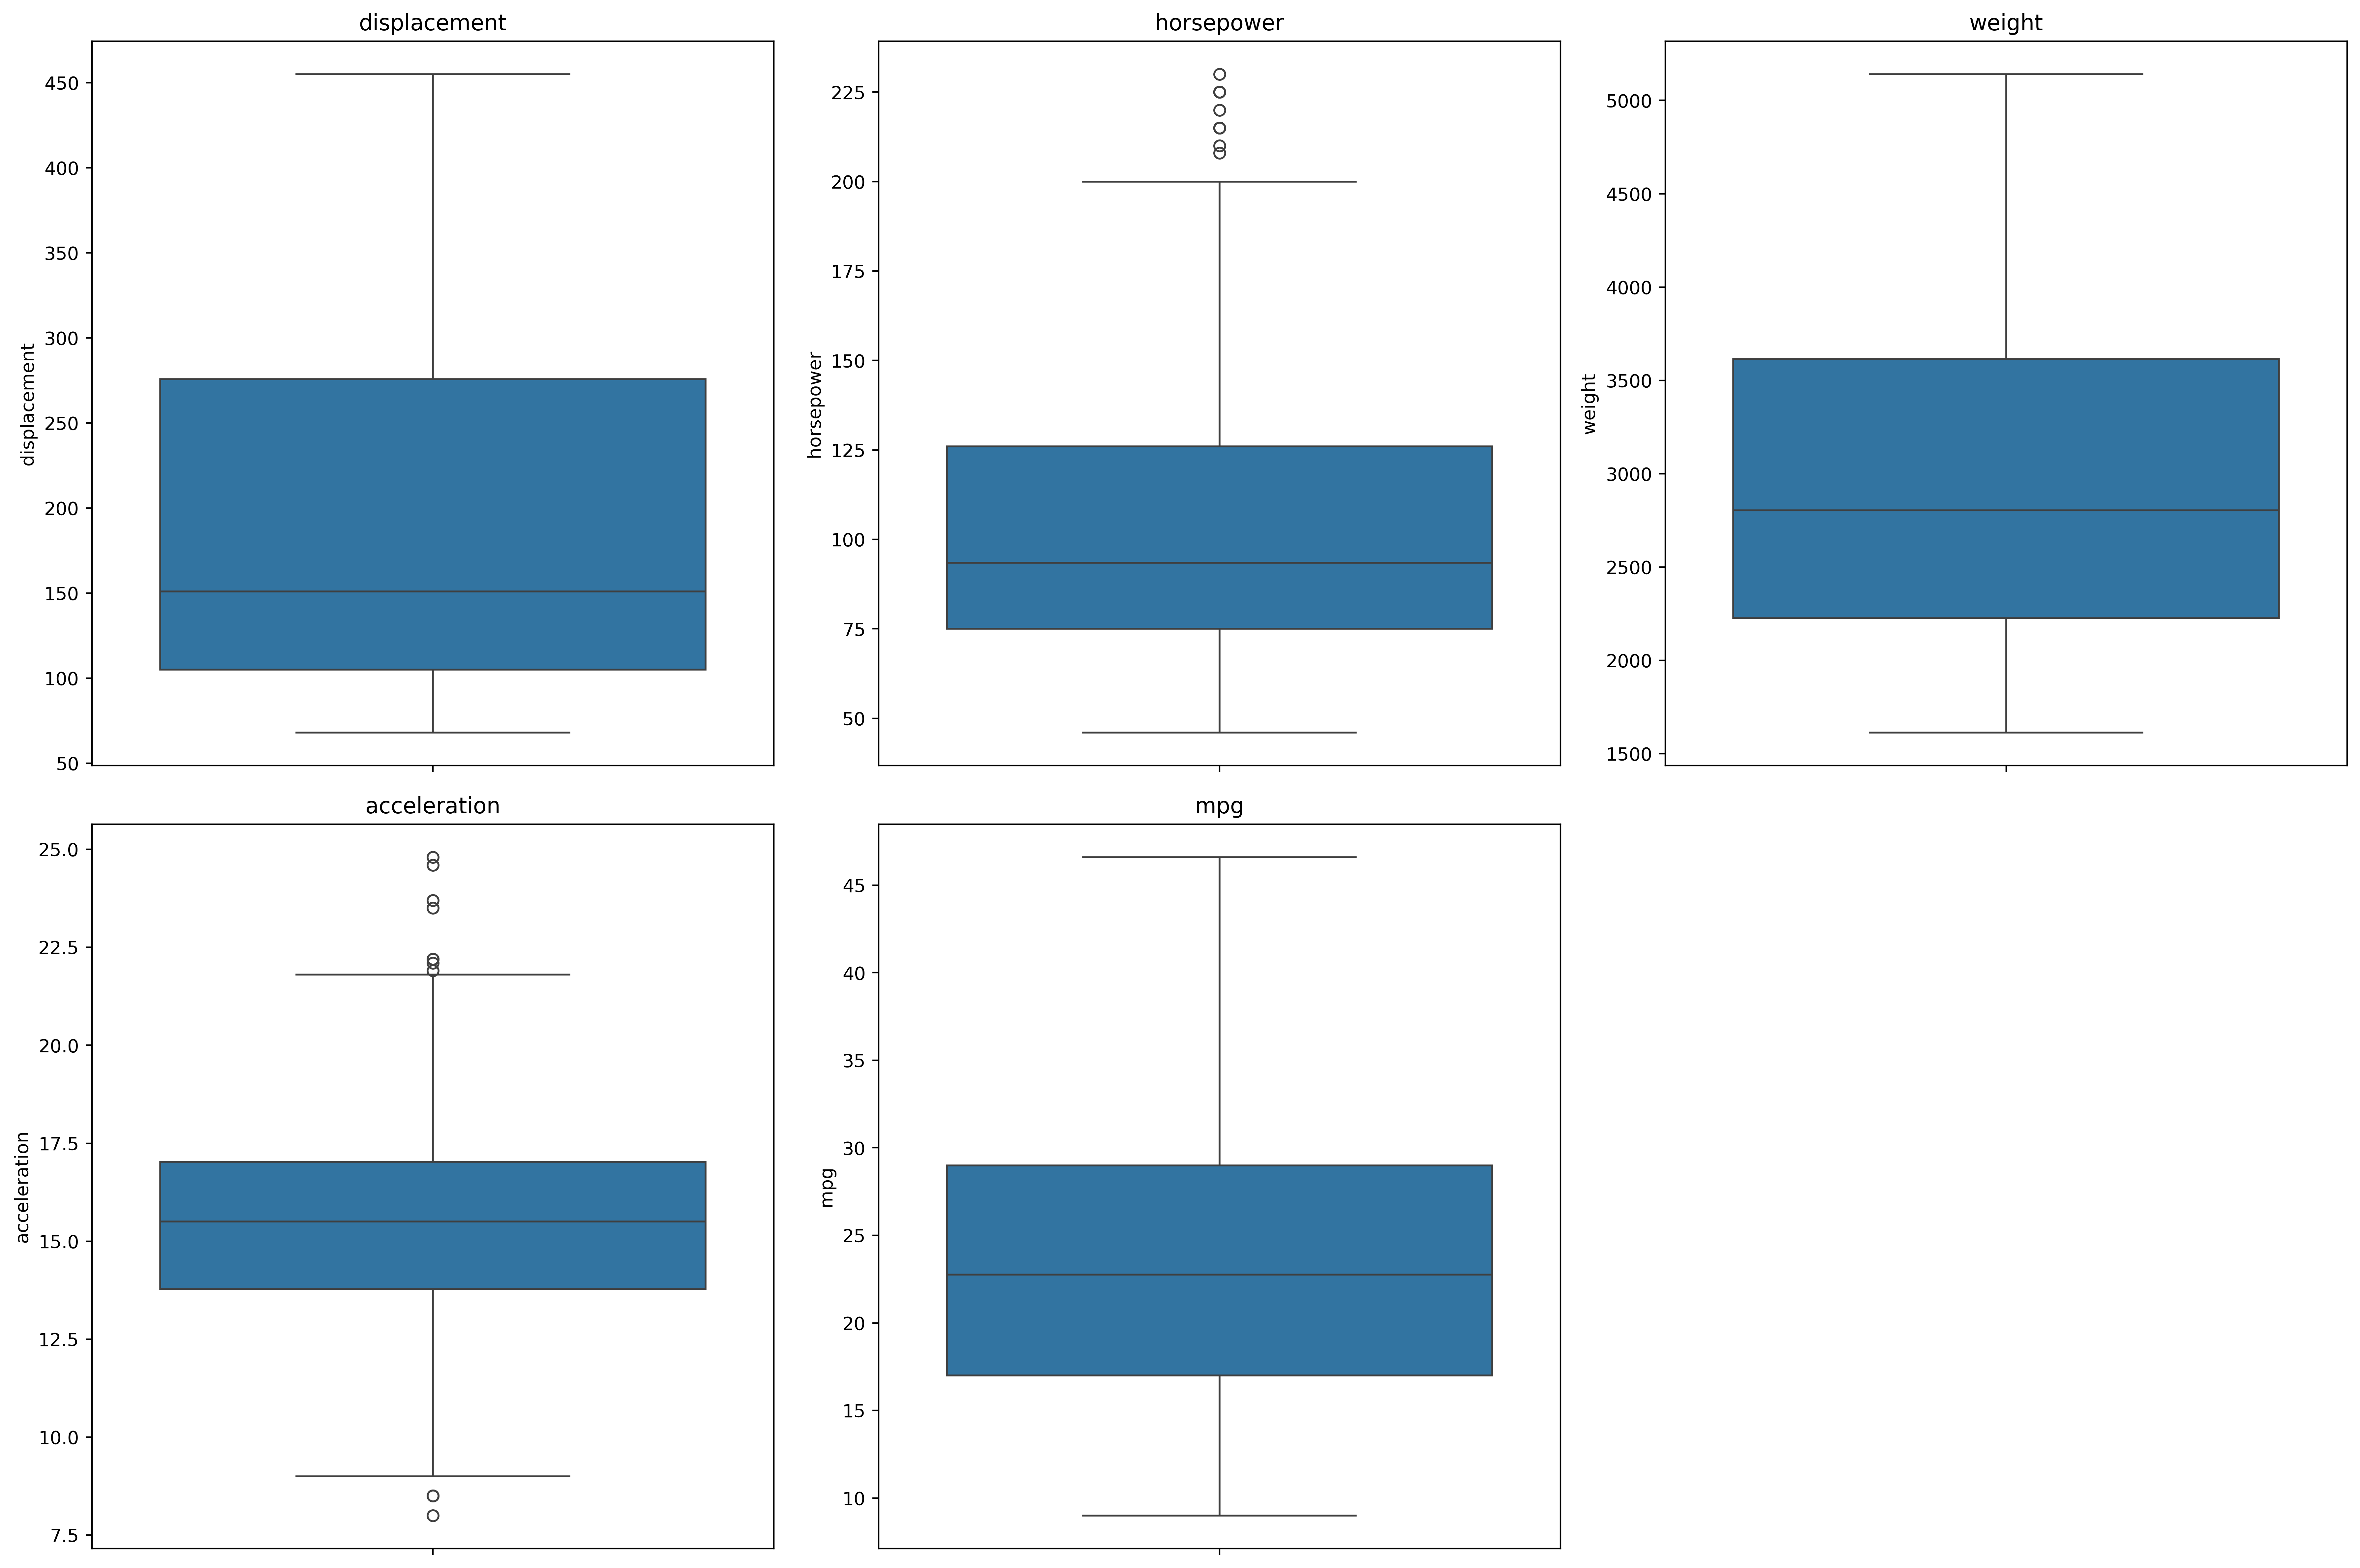
\includegraphics[width=0.75\textwidth]{../Auto_MPG/boxplots.png} 
    \caption{Auto MPG Box Plots}
    \label{fig:Auto MPG Box Plots}
\end{figure}

\Cref{fig:Auto MPG Scatterplots} displays the bivariate relationships between each predictor and the target variable, mpg, while the corresponding correlation matrix is provided in \Cref{fig:Auto MPG Correlation Heat Map}. Analysis of these figures indicates that displacement, cylinders, horsepower, and weight share the strongest correlations with mpg. However, these predictors also exhibit high degrees of inter-correlation, suggesting potential multi-collinearity. Furthermore, the scatterplots reveal distinct non-linear trends in the relationships between mpg and the displacement, horsepower, and weight variables.

\begin{figure}[H]
    \centering
    \captionsetup{justification=centering}
    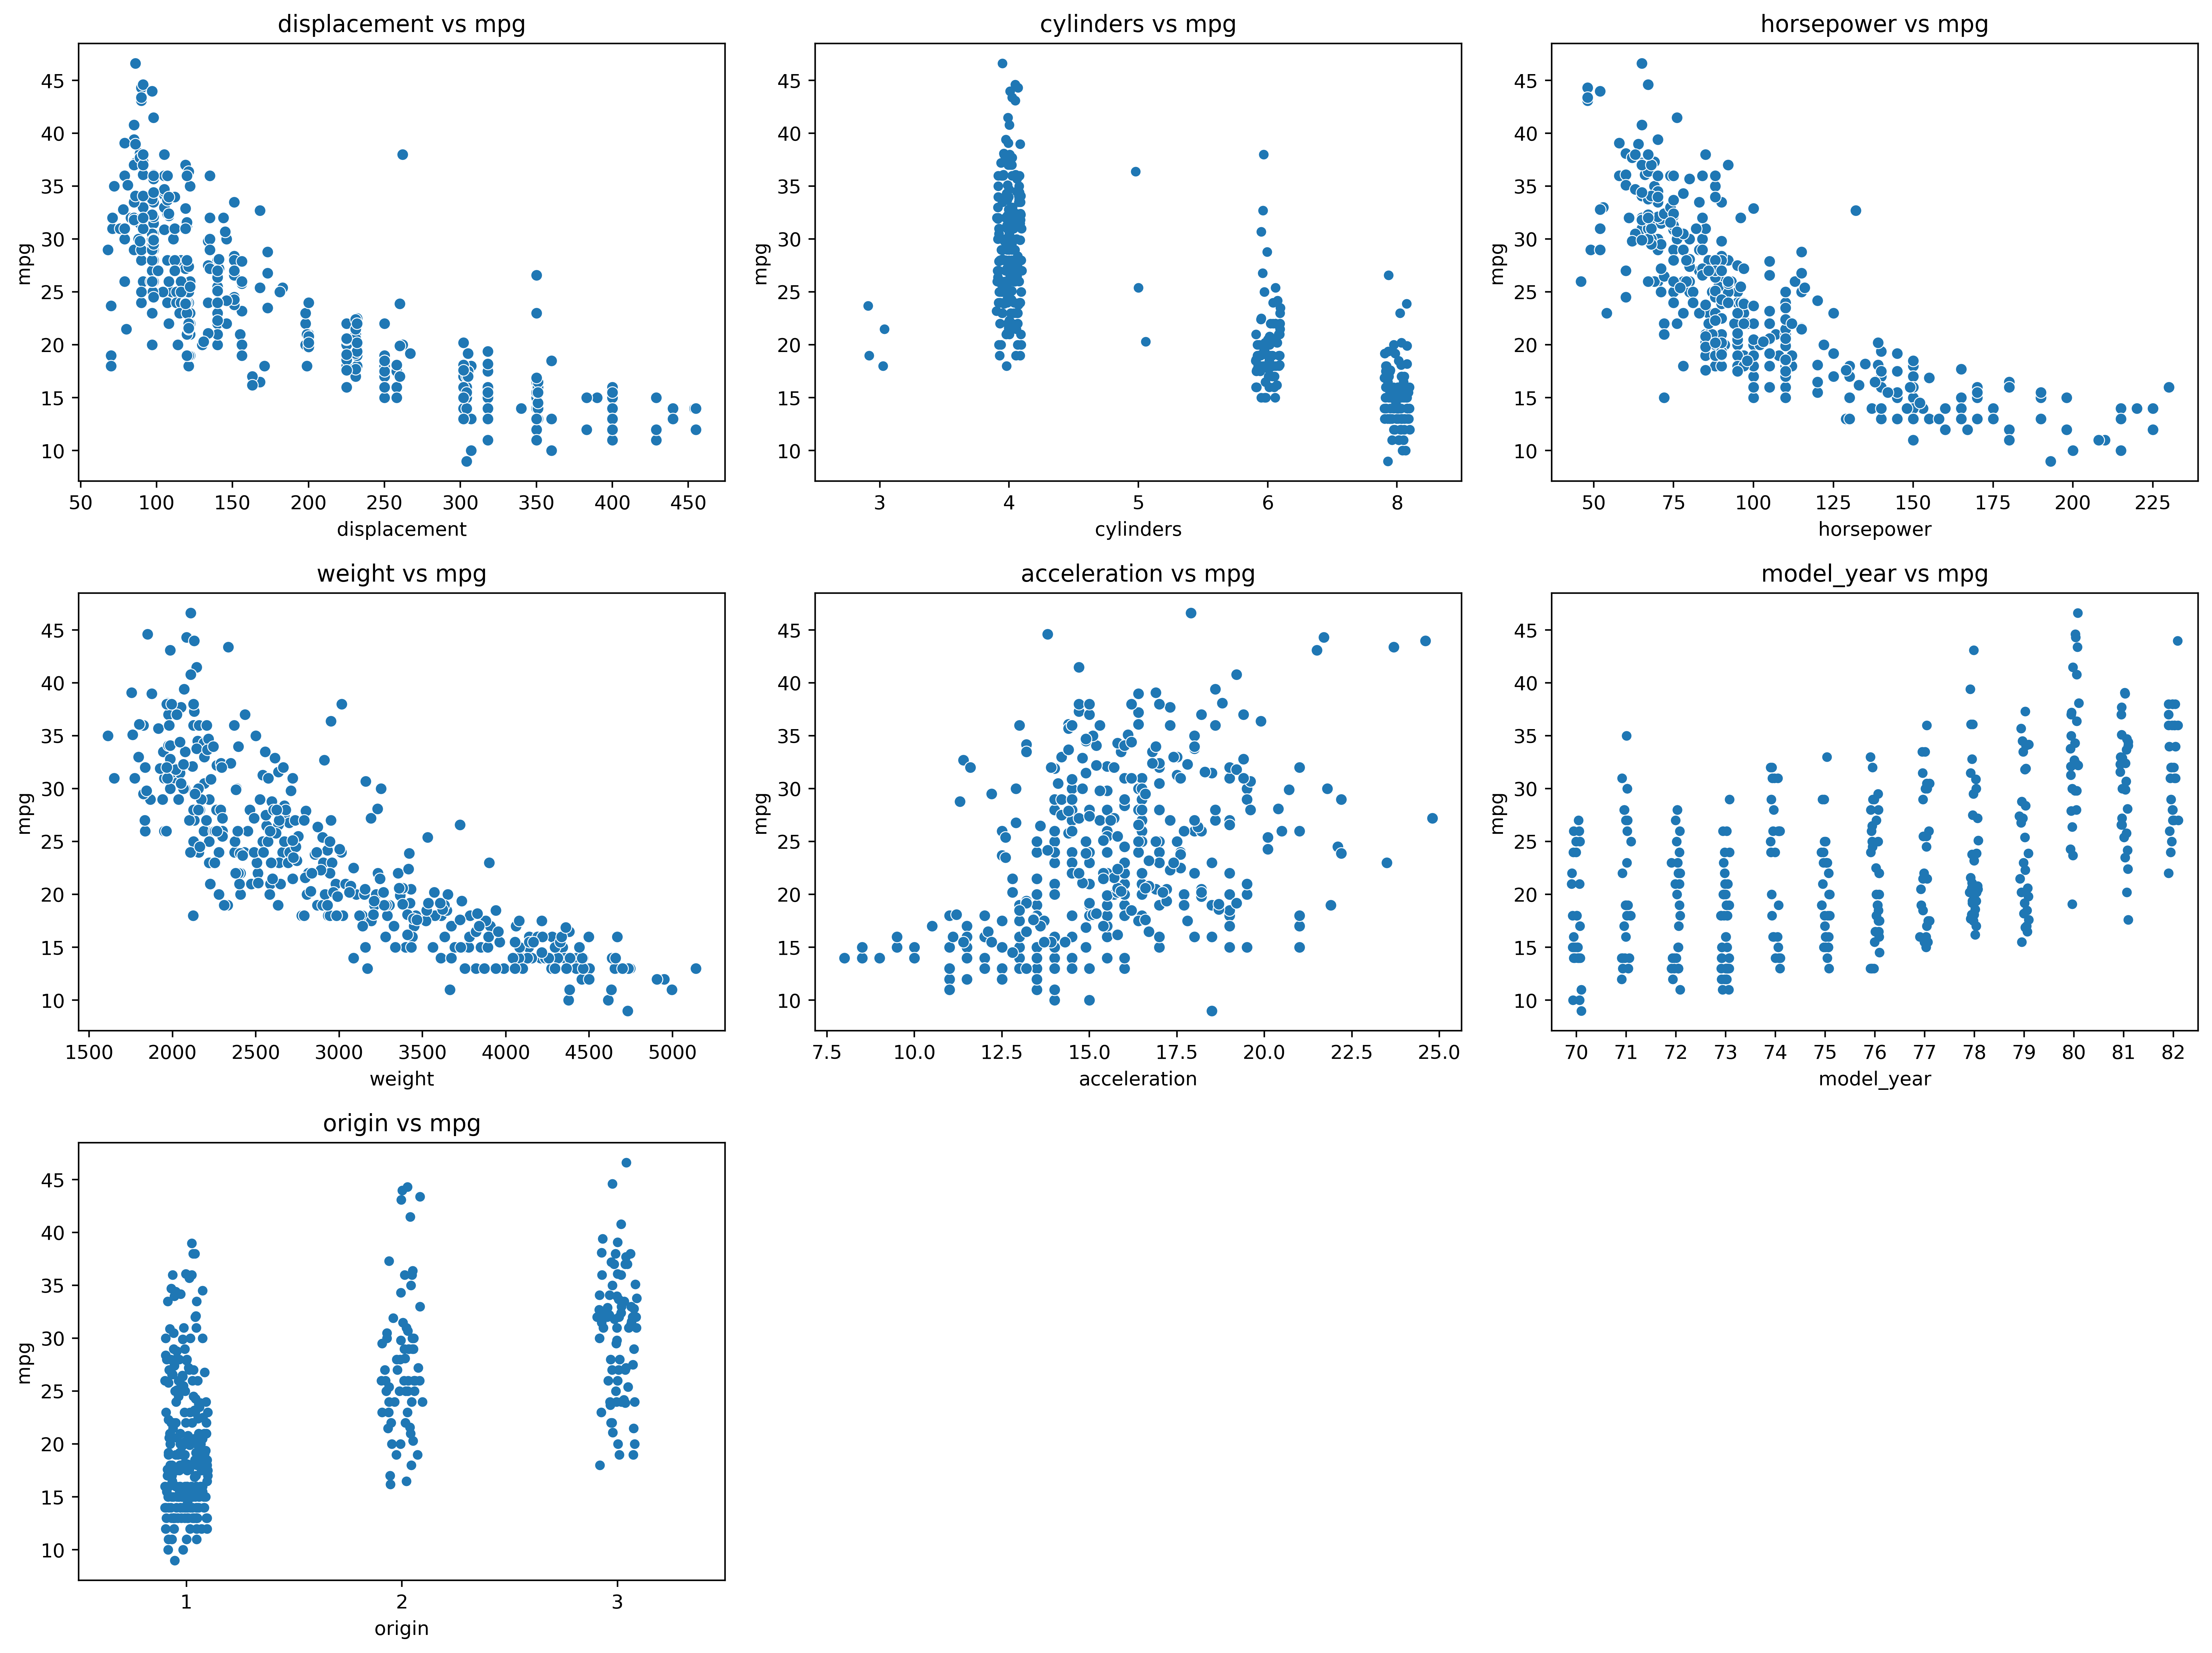
\includegraphics[width=0.75\textwidth]{../Auto_MPG/scatterplots.png} 
    \caption{Auto MPG Scatterplots}
    \label{fig:Auto MPG Scatterplots}
\end{figure}

\begin{figure}[H]
    \centering
    \captionsetup{justification=centering}
    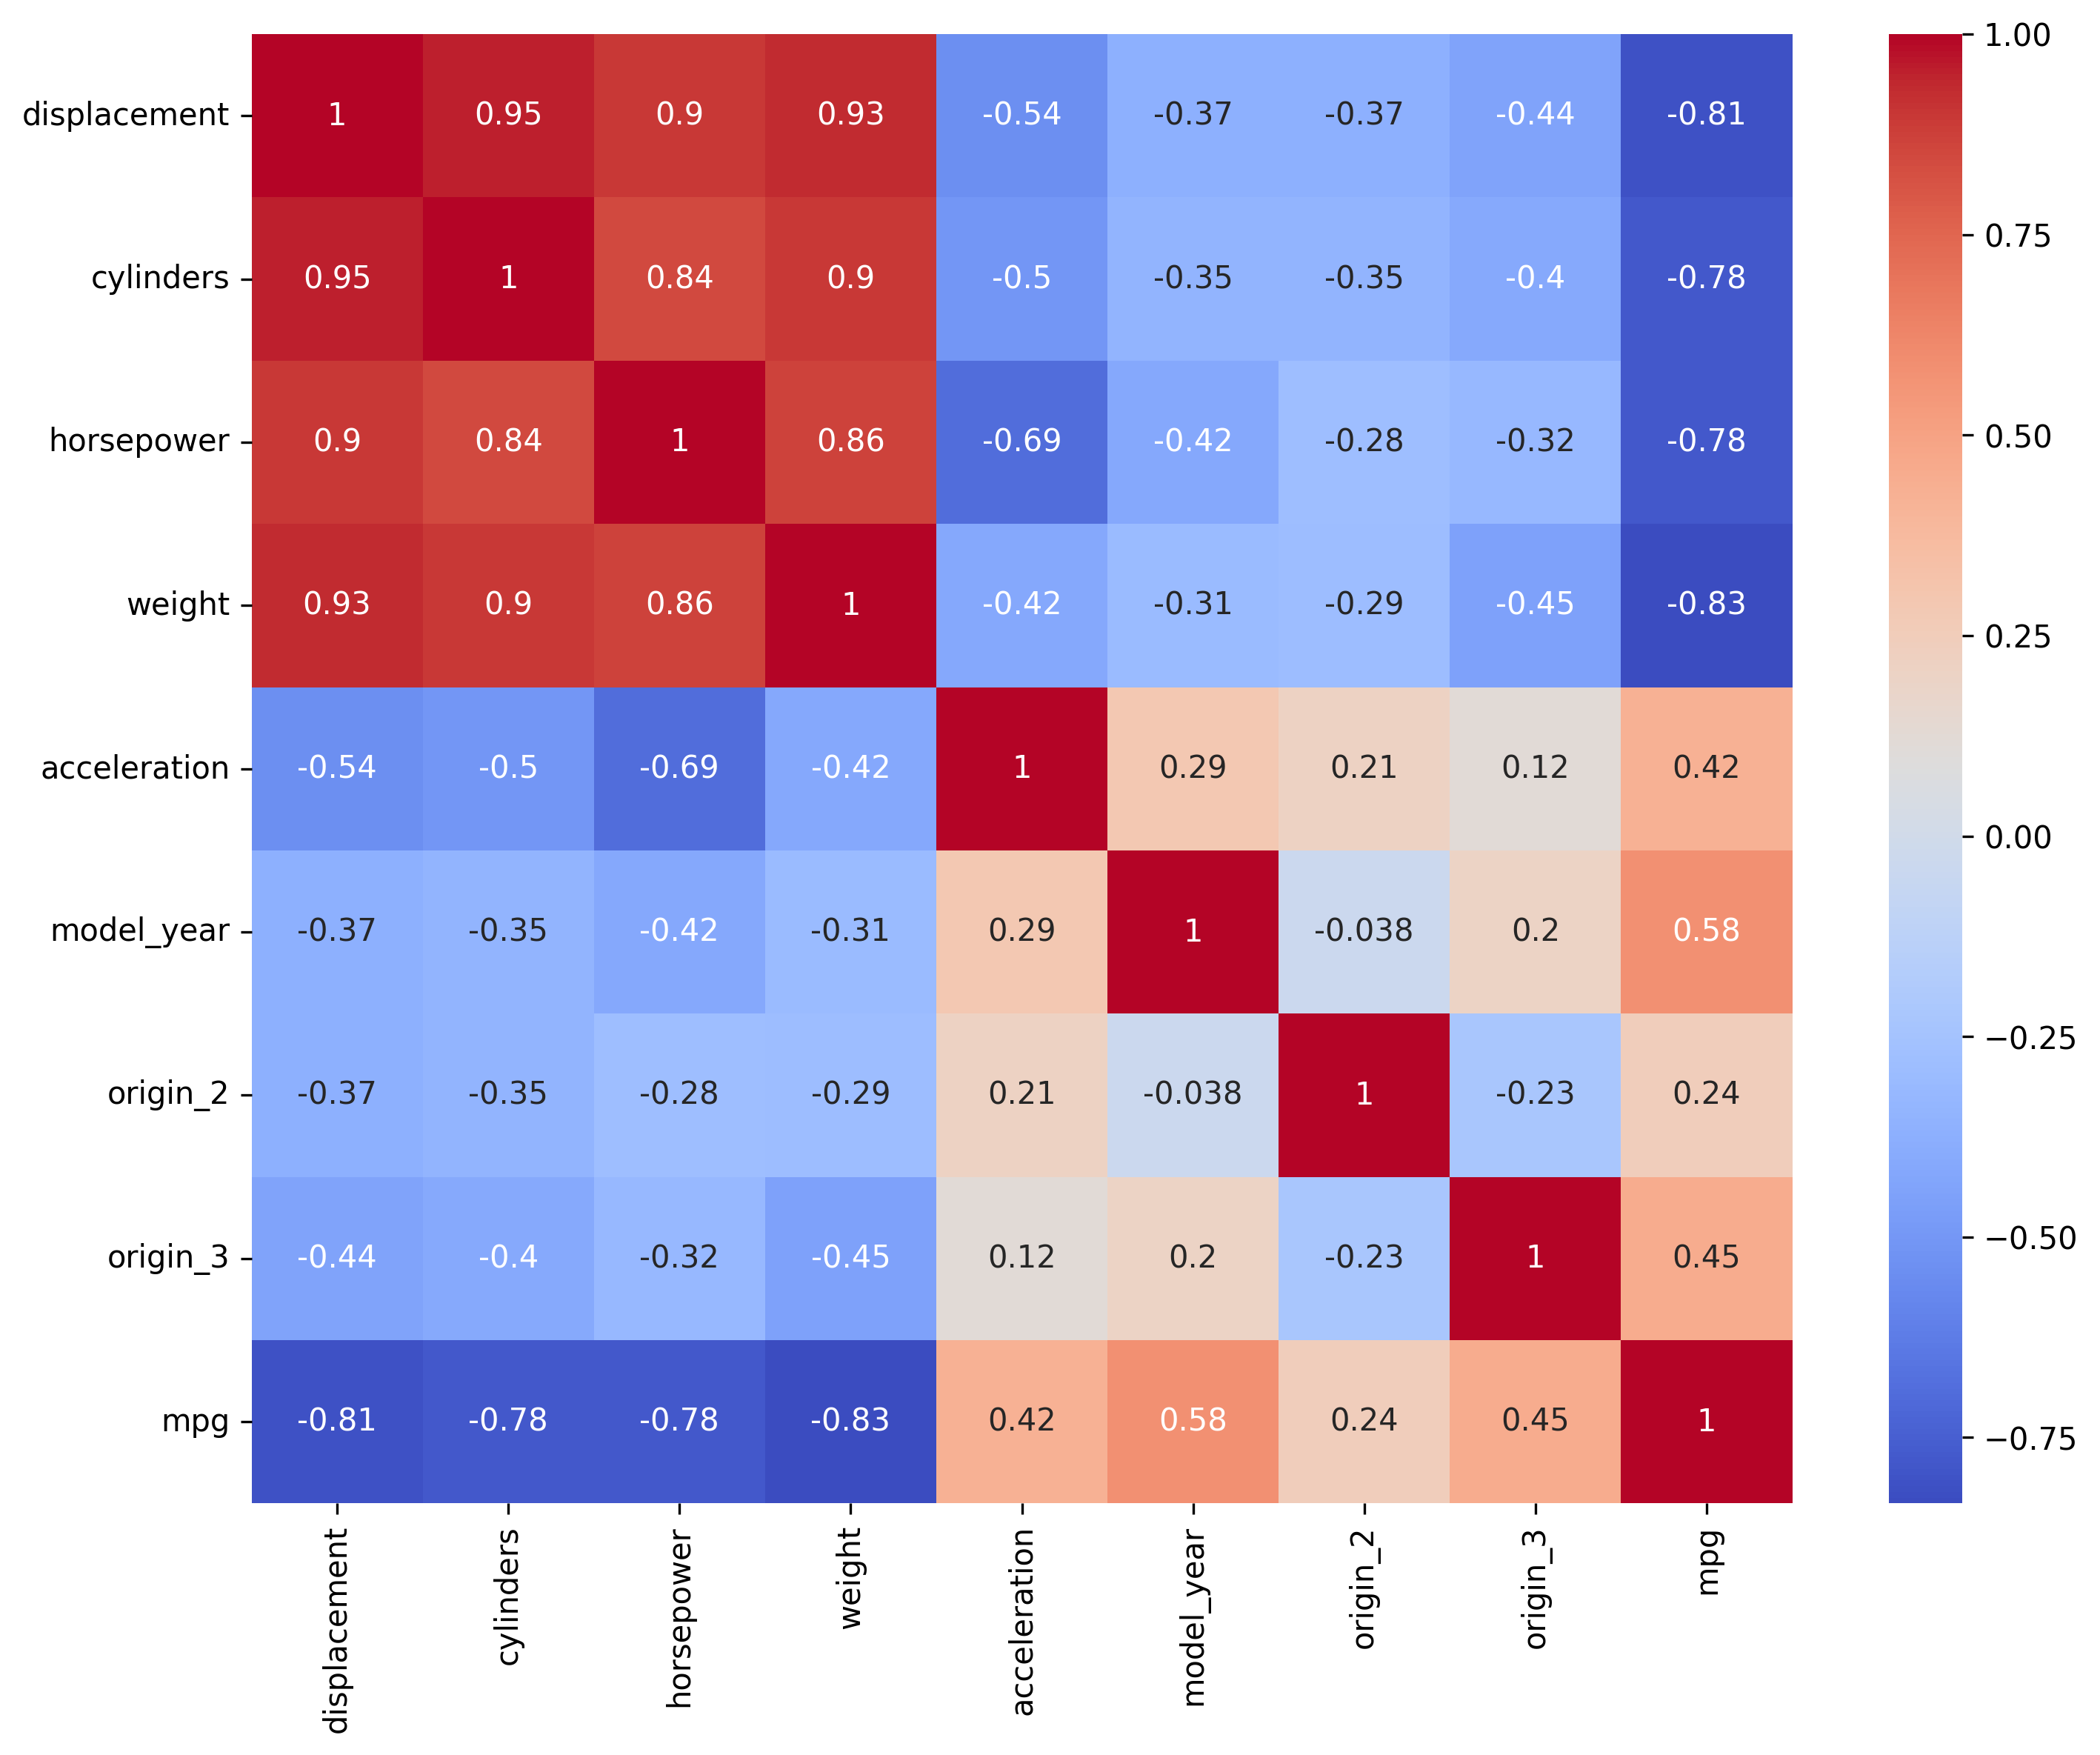
\includegraphics[width=0.5\textwidth]{../Auto_MPG/correlation_heatmap.png} 
    \caption{Auto MPG Correlation Heat Map}
    \label{fig:Auto MPG Correlation Heat Map}
\end{figure}

\Cref{fig:Auto MPG Hue Plots} illustrates the bivariate relationships among the predictor variables, with data points colored by the target variable, mpg. These visualizations further substantiate the high degree of correlation observed between displacement, cylinders, horsepower, and weight. Furthermore, the patterns within these plots suggest that the inclusion of interaction terms may improve model performance. In particular, the relationships between horsepower and model year, as well as weight and model year, indicate significant interactive effects that should be accounted for in the modeling process.

\begin{figure}[H]
    \centering
    \captionsetup{justification=centering}
    \includegraphics[width=0.9\textwidth]{../Auto_MPG/Hue_Plots.png} 
    \caption{Auto MPG Hue Plots}
    \label{fig:Auto MPG Hue Plots}
\end{figure}

\subsection{Multiple Linear Regression}

\subsubsection{Quality of Fit}

\begin{figure}[H]
     \centering
     \captionsetup{justification=centering}
     % First Row
     \begin{subfigure}[b]{0.4\textwidth}
         \centering
         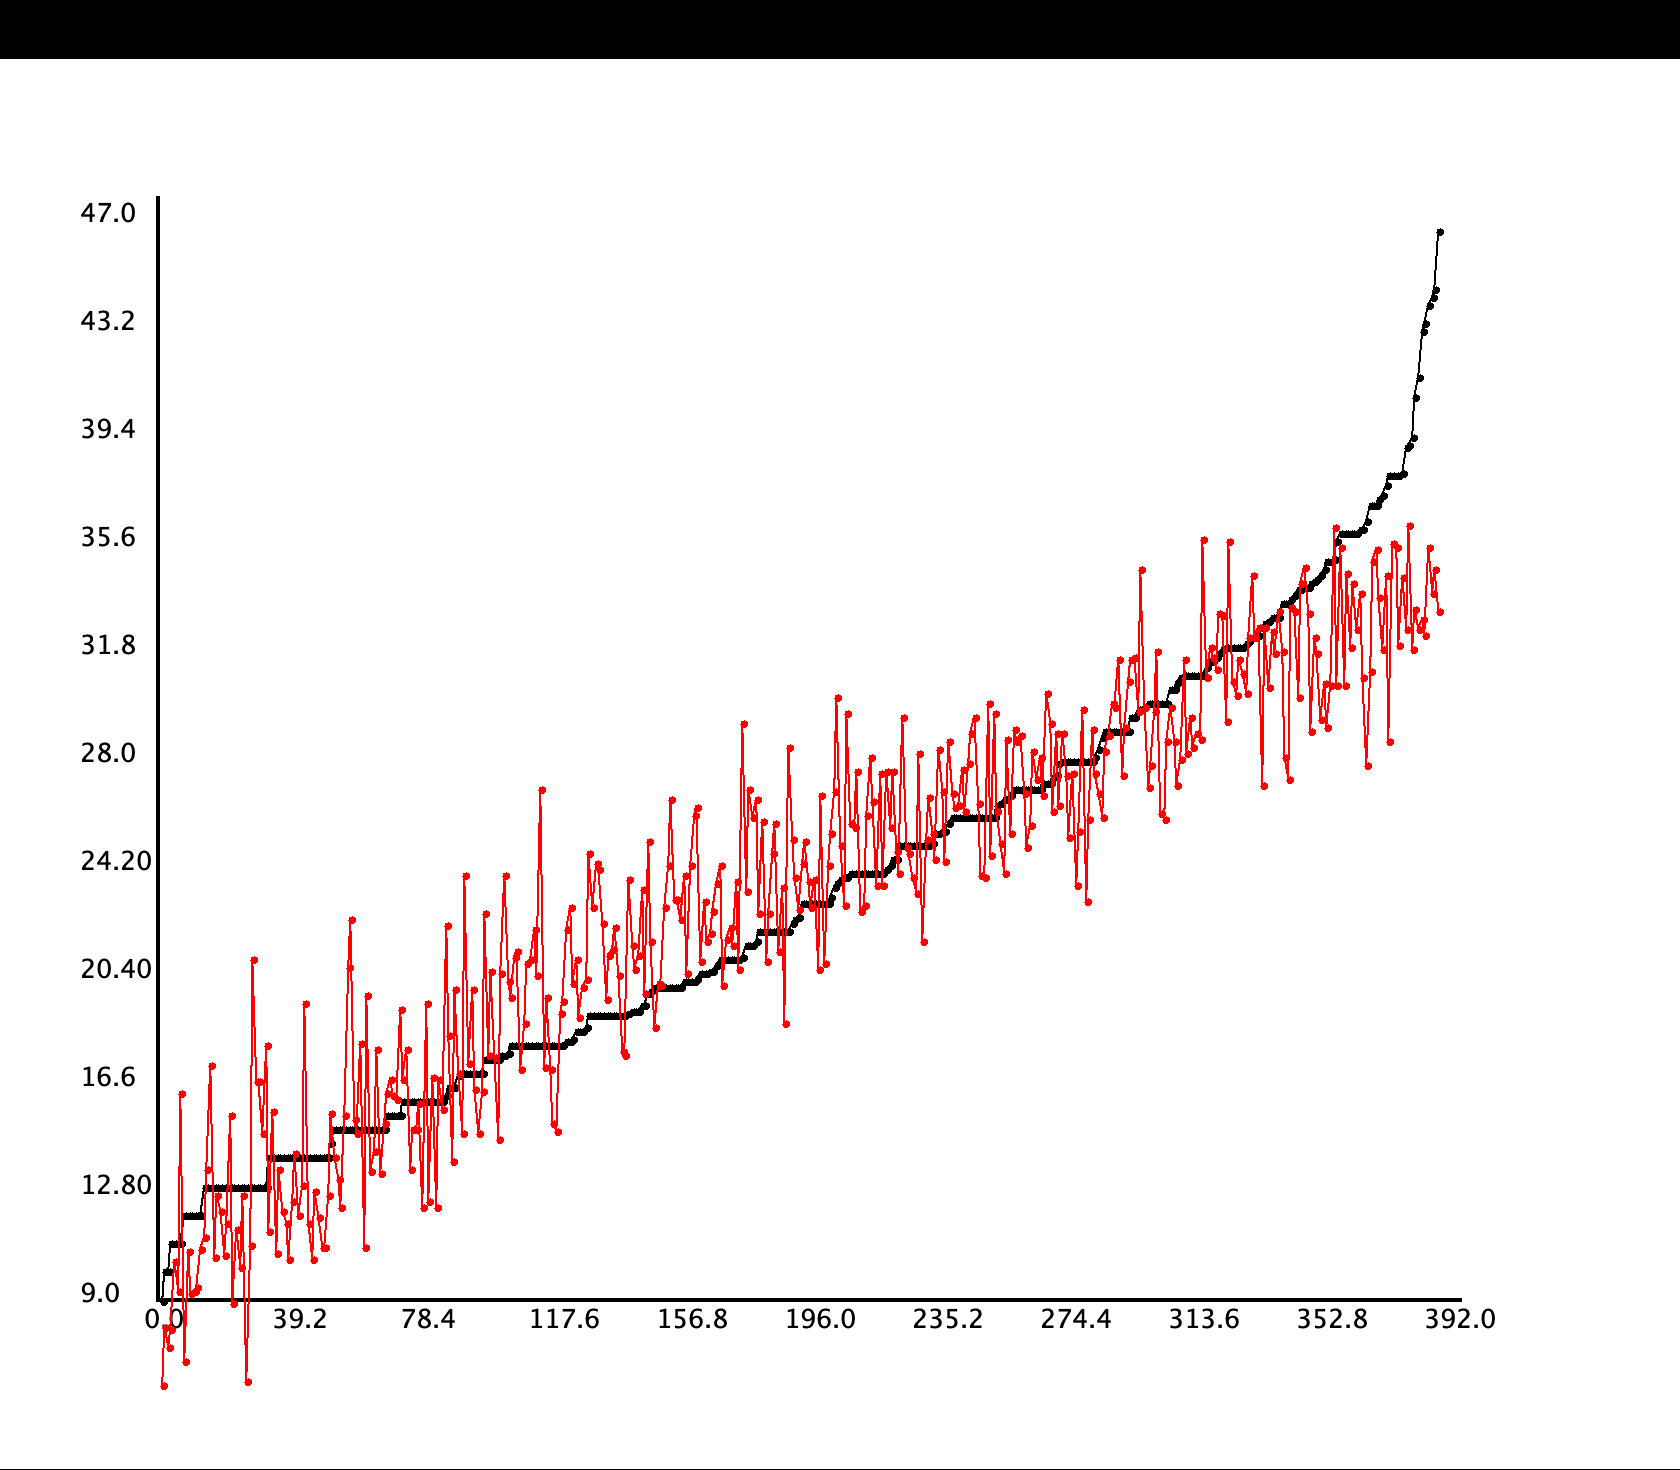
\includegraphics[width=\textwidth]{../Auto_MPG_Scalation_Plots/Scalation_Reg_In_Sample.png}
     \end{subfigure}
     \hfill
     \begin{subfigure}[b]{0.4\textwidth}
         \centering
         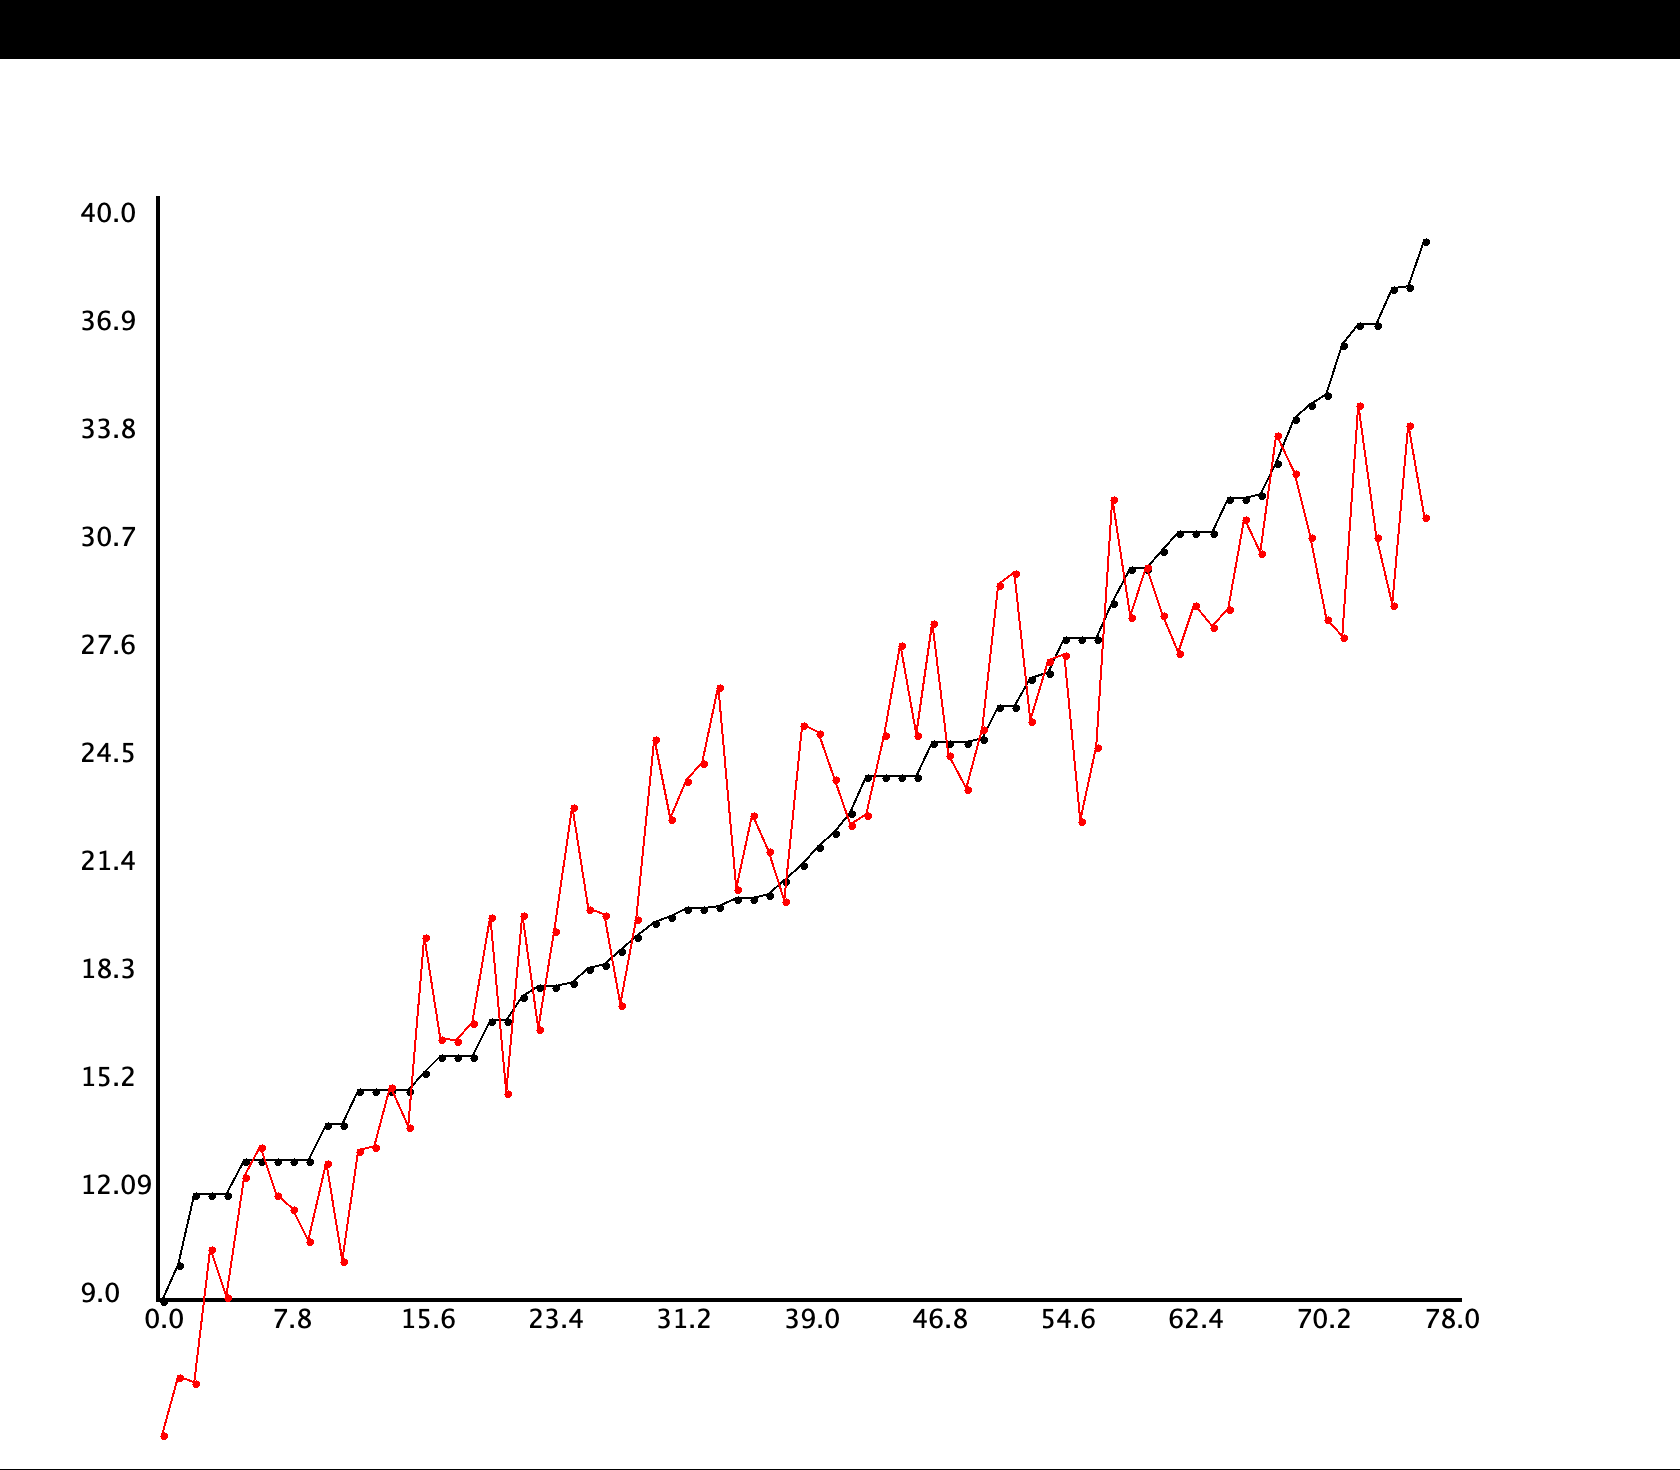
\includegraphics[width=\textwidth]{../Auto_MPG_Scalation_Plots/Scalation_Reg_80_20.png}
     \end{subfigure}

     \vspace{10pt} % Add some vertical spacing between rows

     % Second Row
     \begin{subfigure}[b]{0.49\textwidth}
         \centering
         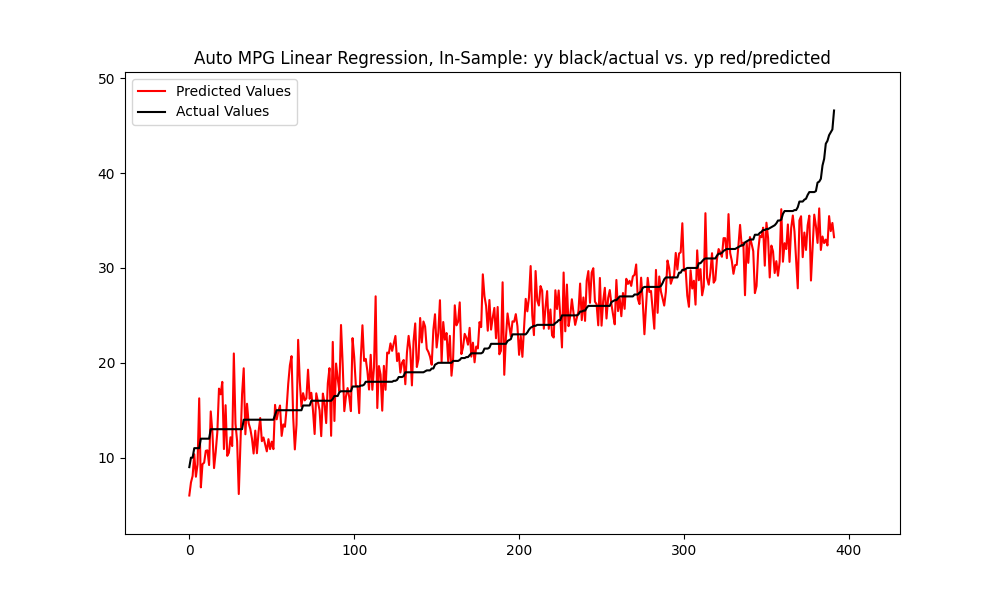
\includegraphics[width=\textwidth]{../Auto_MPG_Statsmodels_Plots/Statsmodels_Reg_In_Sample.png}
     \end{subfigure}
     \hfill
     \begin{subfigure}[b]{0.49\textwidth}
         \centering
         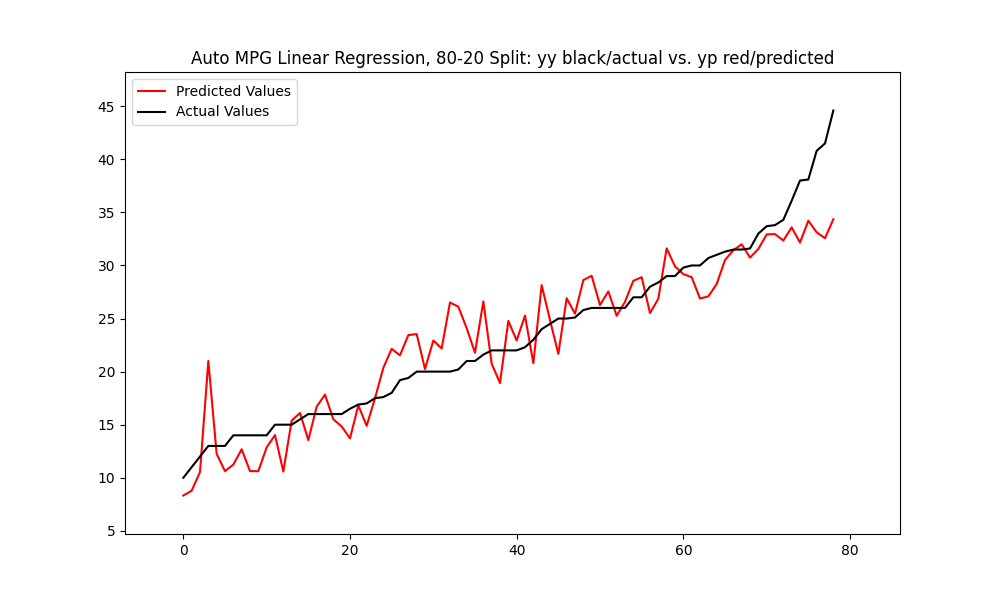
\includegraphics[width=\textwidth]{../Auto_MPG_Statsmodels_Plots/Statsmodels_Reg_80_20.png}
     \end{subfigure}
     
     \caption{Auto MPG Linear Regression Plots\\ Top Left: Scalation In-Sample, Top Right: Scalation Out-of-Sample\\ Bottom Left: Statsmodels In-Sample, Bottom Right: Statsmodels Out-of-Sample\\ black: actual y-values, red: predicted y-values}
     \label{fig:Auto MPG Linear Regression Plots}
\end{figure}

\begin{table}[H]
\centering
\caption{Scalation - Auto MPG Linear Regression}
\label{tab:Scalation - Auto MPG Linear Regression}
\begin{tabular}{|c|c|c|} \hline 
Metric & In-Sample & 80-20 Split \\ \hline \hline 
rSq &0.824199 & 0.831869 \\ \hline 
rSqBar &0.820527 &      0.828357 \\ \hline 
sst &23819.0 &  4731.23 \\ \hline 
sse &4187.39 &  795.466 \\ \hline 
sde &3.27253 &  3.17705 \\ \hline 
mse0 &10.6821 & 10.1983 \\ \hline 
rmse &3.26835 & 3.19347 \\ \hline 
mae &2.50539 &  2.49923 \\ \hline 
smape &11.5405 &        12.1086 \\ \hline 
m &392.000 &    78.0000 \\ \hline 
dfr &8.00000 &  8.00000 \\ \hline 
df &383.000 &   383.000 \\ \hline 
fStat &224.451 &        236.874 \\ \hline 
aic &-1002.46 & -183.254 \\ \hline 
bic &-966.723 & -162.044 \\ \hline 
\end{tabular}
\end{table}

\begin{table}[H]
\centering
\caption{Statsmodels - Auto MPG Linear Regression}
\label{tab:Statsmodels - Auto MPG Linear Regression}
\begin{tabular}{|c|c|c|}\hline
Metric & In-Sample & 80-20 Split \\ \hline \hline
rSq & 0.8242 & 0.8388 \\ \hline
rSqBar & 0.8205 & 0.8203 \\ \hline
sst & 23818.9935 & 4910.2699 \\ \hline
sse & 4187.3917 & 791.7715 \\ \hline
sde & 3.3065 & 3.3632 \\ \hline
mse0 & 10.9331 & 10.0224 \\ \hline
rmse & 3.3065 & 3.1658 \\ \hline
mae & 2.5054 & 2.4149 \\ \hline
smape & 11.5405 & 11.1538 \\ \hline
m & 392.0000 & 79.0000 \\ \hline
dfr & 8.0000 & 9.0000 \\ \hline
df & 383.0000 & 70.0000 \\ \hline
fStat & 224.4507 & 40.4571 \\ \hline
aic & 2058.9278 & 200.0812 \\ \hline
bic & 2094.6692 & 221.4062 \\ \hline
\end{tabular}
\end{table}

\begin{table}[H]
\centering
\caption{Scalation - Auto MPG Linear Regression CV}
\label{tab:Scalation - Auto MPG Linear Regression CV}
\begin{tabular}{|c|c|c|c|c|c|}\hline
Metric & num folds & min & max & mean & stdev \\ \hline \hline
rSq & 5 & 0.783 & 0.832 & 0.808 & 0.018 \\ \hline
rSqBar & 5 & 0.779 & 0.828 & 0.804 & 0.018 \\ \hline
sst & 5 & 3962.818 & 5671.580 & 4700.481 & 620.767 \\ \hline
sse & 5 & 775.125 & 1045.947 & 898.143 & 114.679 \\ \hline
sde & 5 & 3.018 & 3.516 & 3.326 & 0.218 \\ \hline
mse0 & 5 & 9.937 & 13.410 & 11.515 & 1.470 \\ \hline
rmse & 5 & 3.152 & 3.662 & 3.388 & 0.216 \\ \hline
mae & 5 & 2.479 & 2.763 & 2.585 & 0.114 \\ \hline
smape & 5 & 11.299 & 12.413 & 11.891 & 0.501 \\ \hline
m & 5 & 78.000 & 78.000 & 78.000 & 0.000 \\ \hline
dfr & 5 & 8.000 & 8.000 & 8.000 & 0.000 \\ \hline
df & 5 & 383.000 & 383.000 & 383.000 & 0.000 \\ \hline
fStat & 5 & 173.074 & 236.874 & 203.481 & 23.306 \\ \hline
aic & 5 & -195.823 & -182.234 & -188.407 & 5.755 \\ \hline
bic & 5 & -174.613 & -161.023 & -167.196 & 5.755 \\ \hline
\end{tabular}
\end{table}

\begin{table}[H]
\centering
\caption{Statsmodels - Auto MPG Linear Regression CV}
\label{tab:Statsmodels - Auto MPG Linear Regression CV}
\begin{tabular}{|c|c|c|c|c|c|}\hline
Metric & num folds & min & max & mean & stdev \\ \hline \hline
rSq & 5 & 0.7157 & 0.8442 & 0.8062 & 0.0467 \\ \hline
rSqBar & 5 & 0.6828 & 0.8262 & 0.7839 & 0.0521 \\ \hline
sst & 5 & 3880.9704 & 5093.9237 & 4721.1782 & 441.3031 \\ \hline
sse & 5 & 791.7715 & 1103.1742 & 895.0561 & 115.5640 \\ \hline
sde & 5 & 3.3632 & 3.9985 & 3.5846 & 0.2331 \\ \hline
mse0 & 5 & 10.0224 & 14.1433 & 11.4215 & 1.5145 \\ \hline
rmse & 5 & 3.1658 & 3.7608 & 3.3725 & 0.2186 \\ \hline
mae & 5 & 2.3886 & 3.0767 & 2.5894 & 0.2538 \\ \hline
smape & 5 & 10.6546 & 14.6636 & 11.9879 & 1.4173 \\ \hline
m & 5 & 78.0000 & 79.0000 & 78.4000 & 0.4899 \\ \hline
dfr & 5 & 9.0000 & 9.0000 & 9.0000 & 0.0000 \\ \hline
df & 5 & 69.0000 & 70.0000 & 69.4000 & 0.4899 \\ \hline
fStat & 5 & 19.3047 & 41.5548 & 33.9820 & 7.9415 \\ \hline
aic & 5 & 198.9325 & 224.6406 & 208.2629 & 9.3175 \\ \hline
bic & 5 & 220.1429 & 245.8509 & 229.5191 & 9.2930 \\ \hline
\end{tabular}
\end{table}

\subsubsection{Feature Selection}

Scalation Forward Selection: intercept, weight, modelyear, origin 3, origin 2, cylinders, displacement, horsepower, acceleration

Statsmodels Forward Selection: intercept, weight, model year, origin 3, origin 2, displacement, horsepower, cylinders, acceleration

\begin{figure}[H]
     \centering
     \captionsetup{justification=centering}
     % First Row
     \begin{subfigure}[b]{0.4\textwidth}
         \centering
         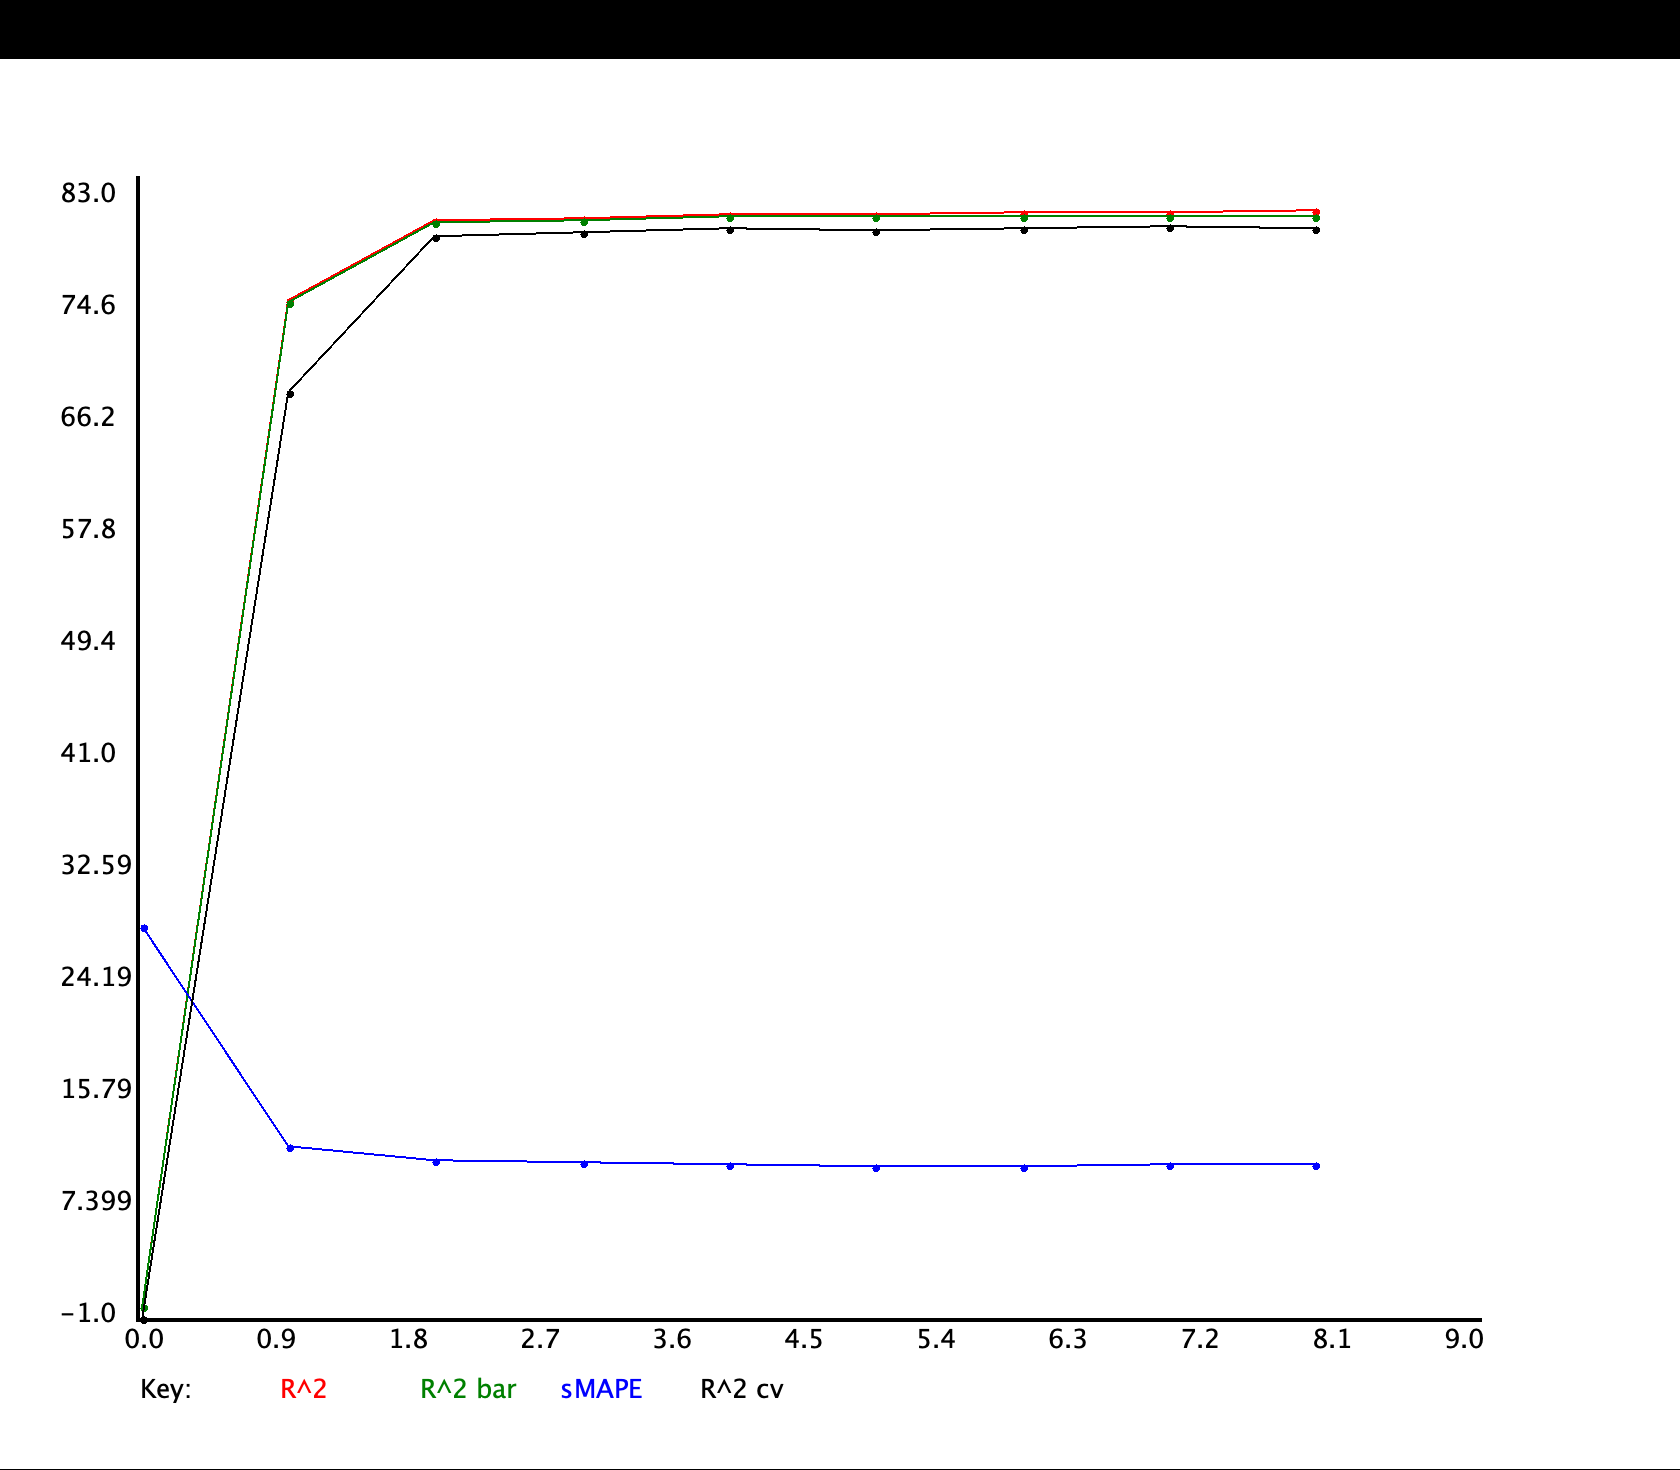
\includegraphics[width=\textwidth]{../Auto_MPG_Scalation_Plots/Scalation_Reg_rSq_Forward.png}
     \end{subfigure}
     \hfill
     \begin{subfigure}[b]{0.4\textwidth}
         \centering
         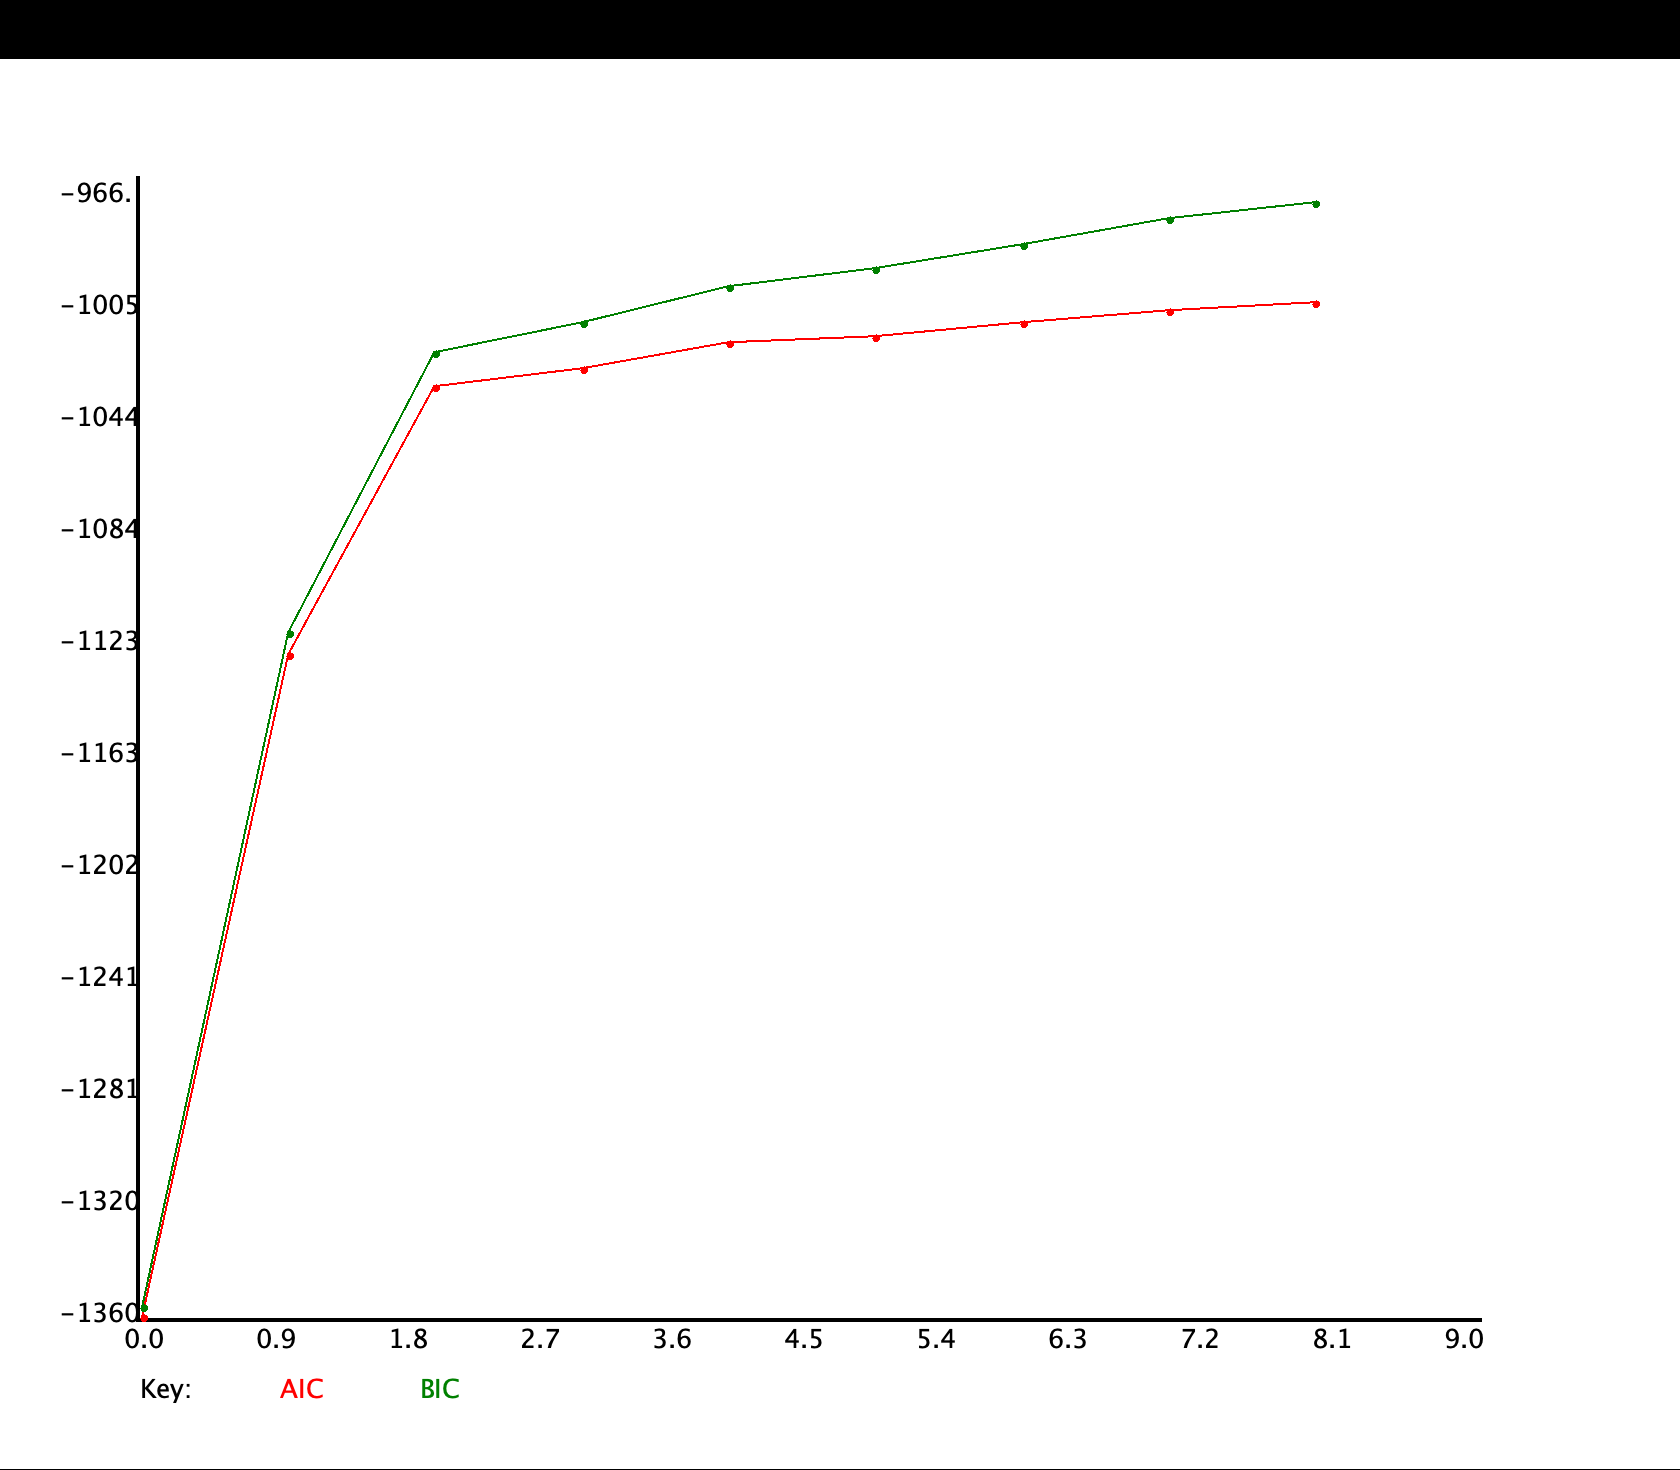
\includegraphics[width=\textwidth]{../Auto_MPG_Scalation_Plots/Scalation_Reg_AIC_BIC_Forward.png}
     \end{subfigure}

     \vspace{10pt} % Add some vertical spacing between rows

     % Second Row
     \begin{subfigure}[b]{0.49\textwidth}
         \centering
         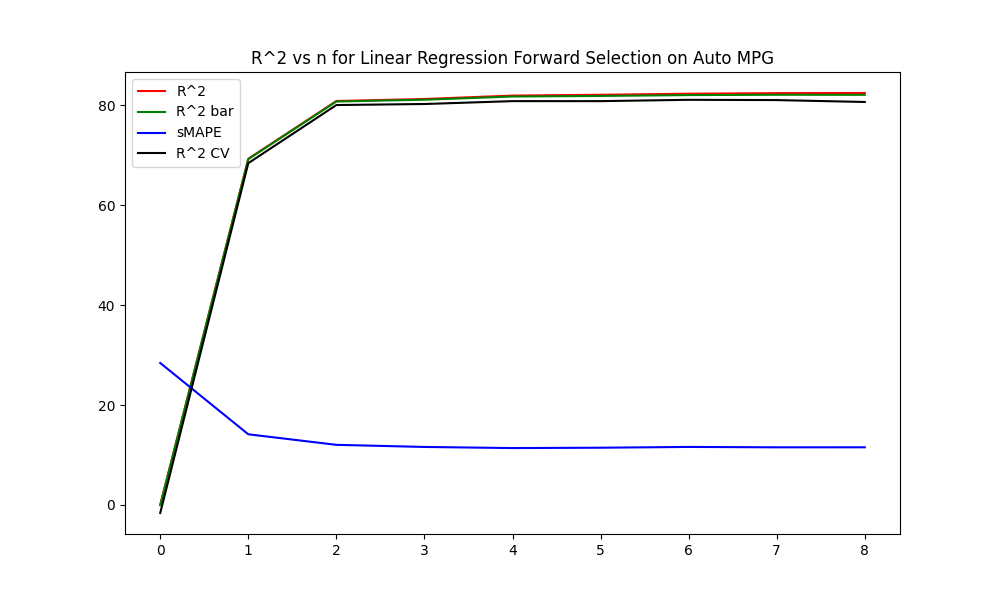
\includegraphics[width=\textwidth]{../Auto_MPG_Statsmodels_Plots/Statsmodels_Reg_rSq_Forward.png}
     \end{subfigure}
     \hfill
     \begin{subfigure}[b]{0.49\textwidth}
         \centering
         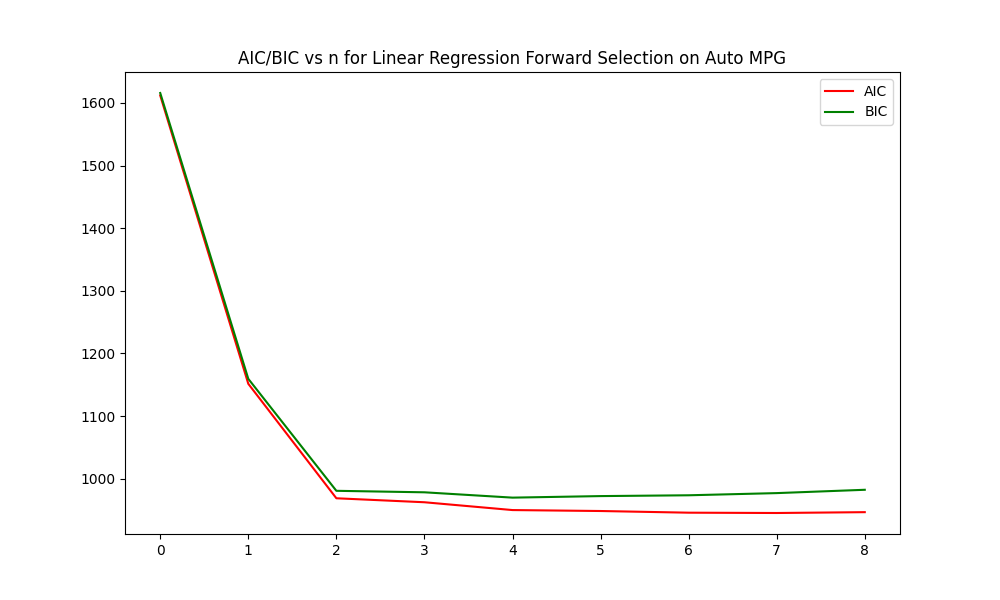
\includegraphics[width=\textwidth]{../Auto_MPG_Statsmodels_Plots/Statsmodels_Reg_AIC_BIC_Forward.png}
     \end{subfigure}
     
     \caption{Auto MPG Linear Regression Forward Selection Quality of Fit Metrics\\ Top Left: Scalation $R^2$, Top Right: Scalation AIC/BIC\\ Bottom Left: Statsmodels $R^2$, Bottom Right: Statsmodels AIC/BIC}
     \label{fig:Auto MPG Linear Regression Forward Selection Quality of Fit Metrics}
\end{figure}

Scalation Backward Elimination Reversed: intercept, weight, modelyear, origin 3, origin 2, cylinders, displacement, horsepower, acceleration

Statsmodels Backward Elimination Reversed: intercept, weight, model year, origin 3, origin 2, displacement, horsepower, cylinders, acceleration

\begin{figure}[H]
     \centering
     \captionsetup{justification=centering}
     % First Row
     \begin{subfigure}[b]{0.4\textwidth}
         \centering
         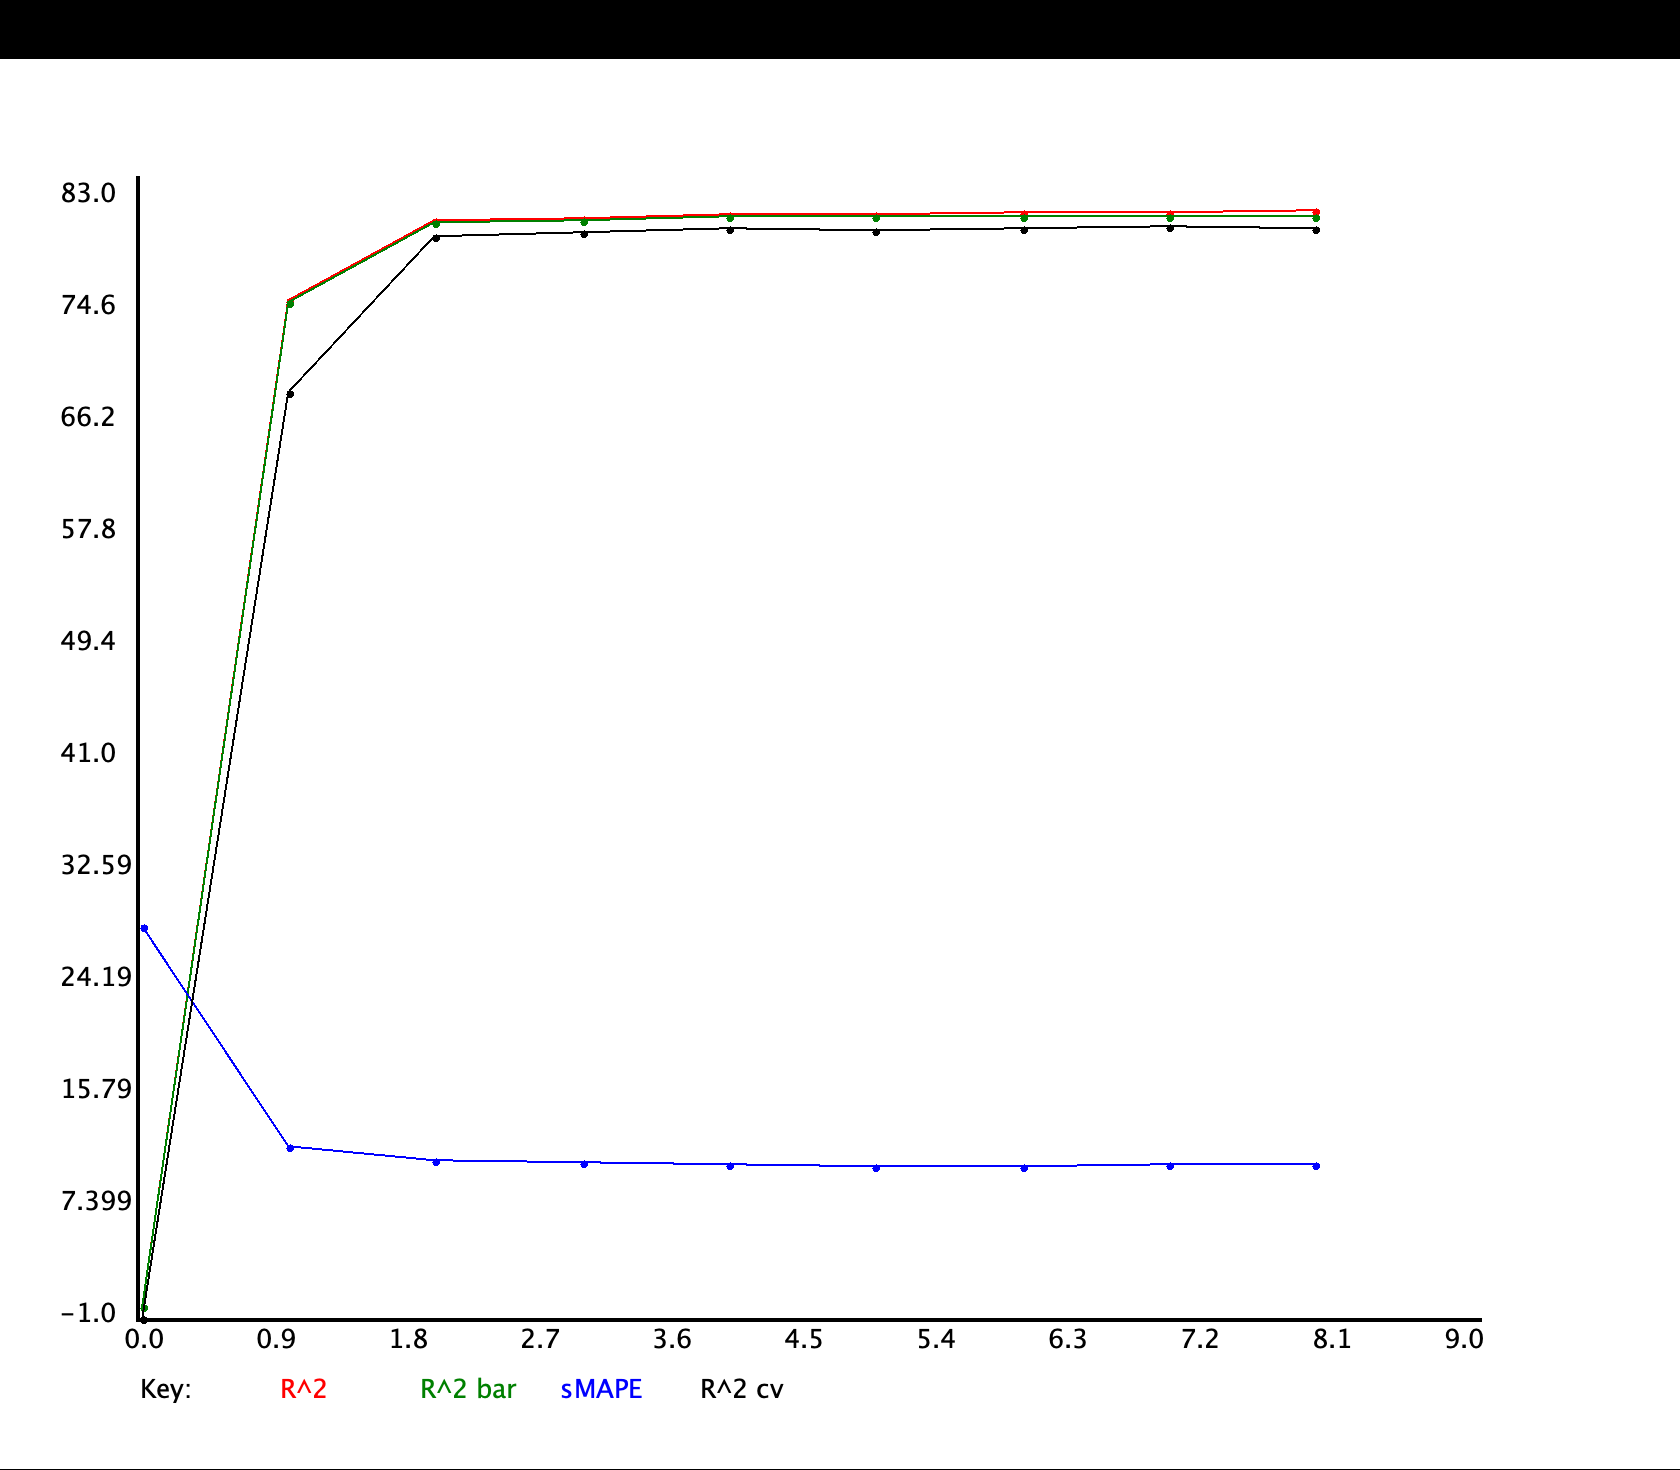
\includegraphics[width=\textwidth]{../Auto_MPG_Scalation_Plots/Scalation_Reg_rSq_Backward.png}
     \end{subfigure}
     \hfill
     \begin{subfigure}[b]{0.4\textwidth}
         \centering
         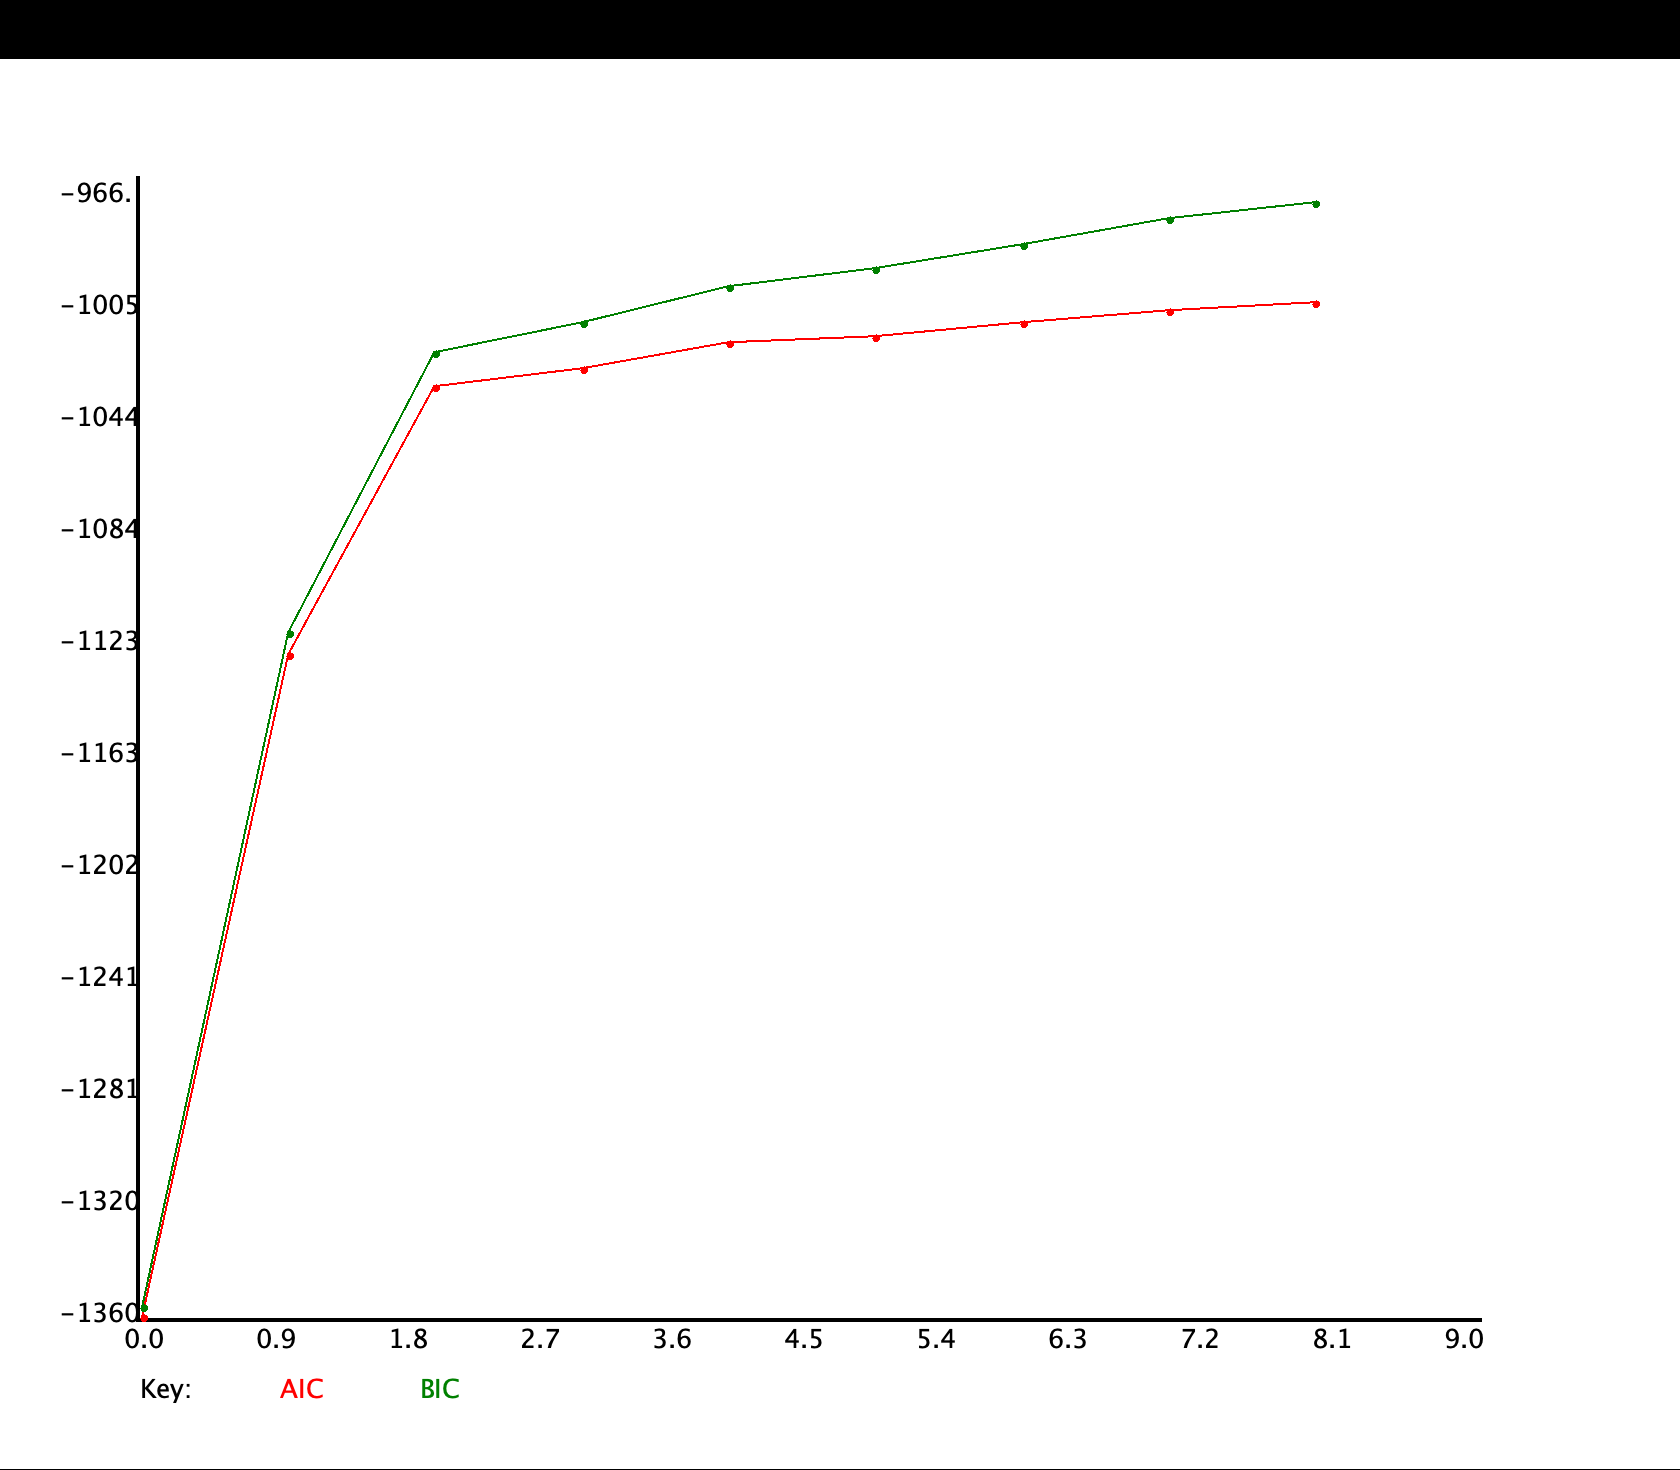
\includegraphics[width=\textwidth]{../Auto_MPG_Scalation_Plots/Scalation_Reg_AIC_BIC_Backward.png}
     \end{subfigure}

     \vspace{10pt} % Add some vertical spacing between rows

     % Second Row
     \begin{subfigure}[b]{0.49\textwidth}
         \centering
         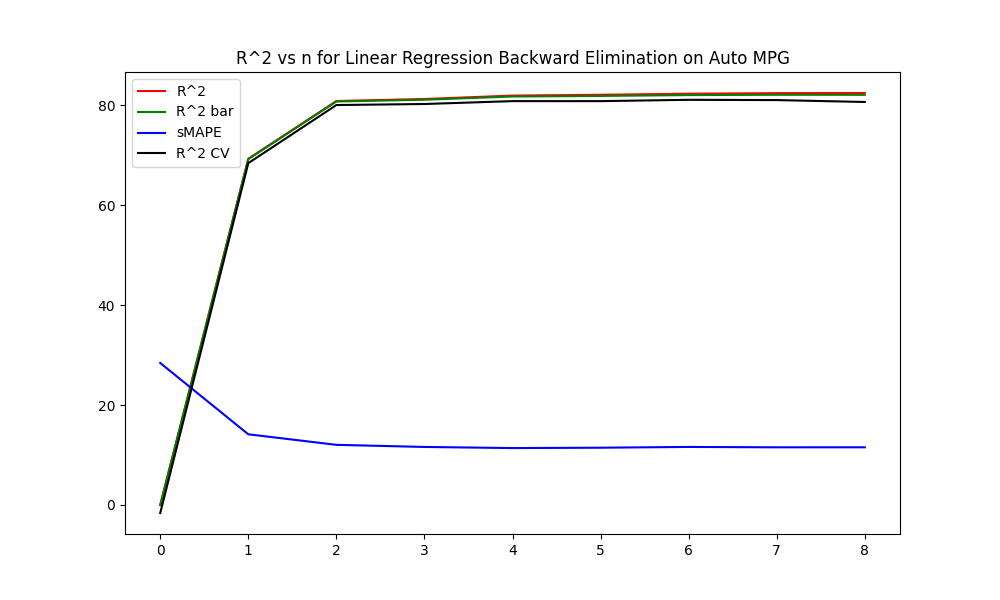
\includegraphics[width=\textwidth]{../Auto_MPG_Statsmodels_Plots/Statsmodels_Reg_rSq_Backward.png}
     \end{subfigure}
     \hfill
     \begin{subfigure}[b]{0.49\textwidth}
         \centering
         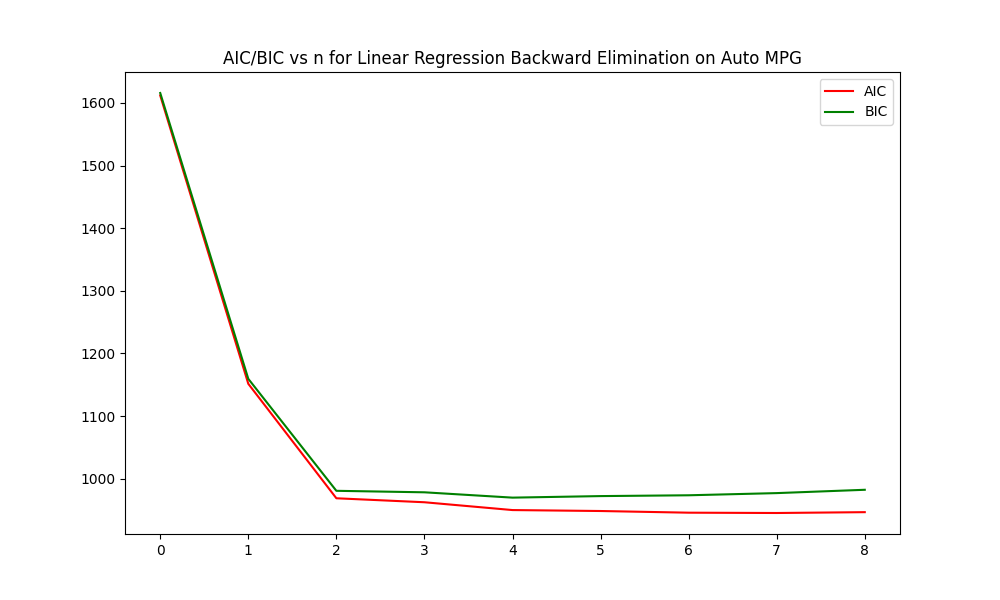
\includegraphics[width=\textwidth]{../Auto_MPG_Statsmodels_Plots/Statsmodels_Reg_AIC_BIC_Backward.png}
     \end{subfigure}
     
     \caption{Auto MPG Linear Regression Reversed Backward Elimination Quality of Fit Metrics\\ Top Left: Scalation $R^2$, Top Right: Scalation AIC/BIC\\ Bottom Left: Statsmodels $R^2$, Bottom Right: Statsmodels AIC/BIC}
     \label{fig:Auto MPG Linear Regression Reversed Backward Elimination Quality of Fit Metrics}
\end{figure}

Scalation Stepwise Selection: intercept, weight, modelyear, origin 3, origin 2, cylinders, displacement, horsepower

Statsmodels Stepwise Selection: intercept, weight, model year, origin 3, origin 2, displacement, horsepower, cylinders

\begin{figure}[H]
     \centering
     \captionsetup{justification=centering}
     % First Row
     \begin{subfigure}[b]{0.4\textwidth}
         \centering
         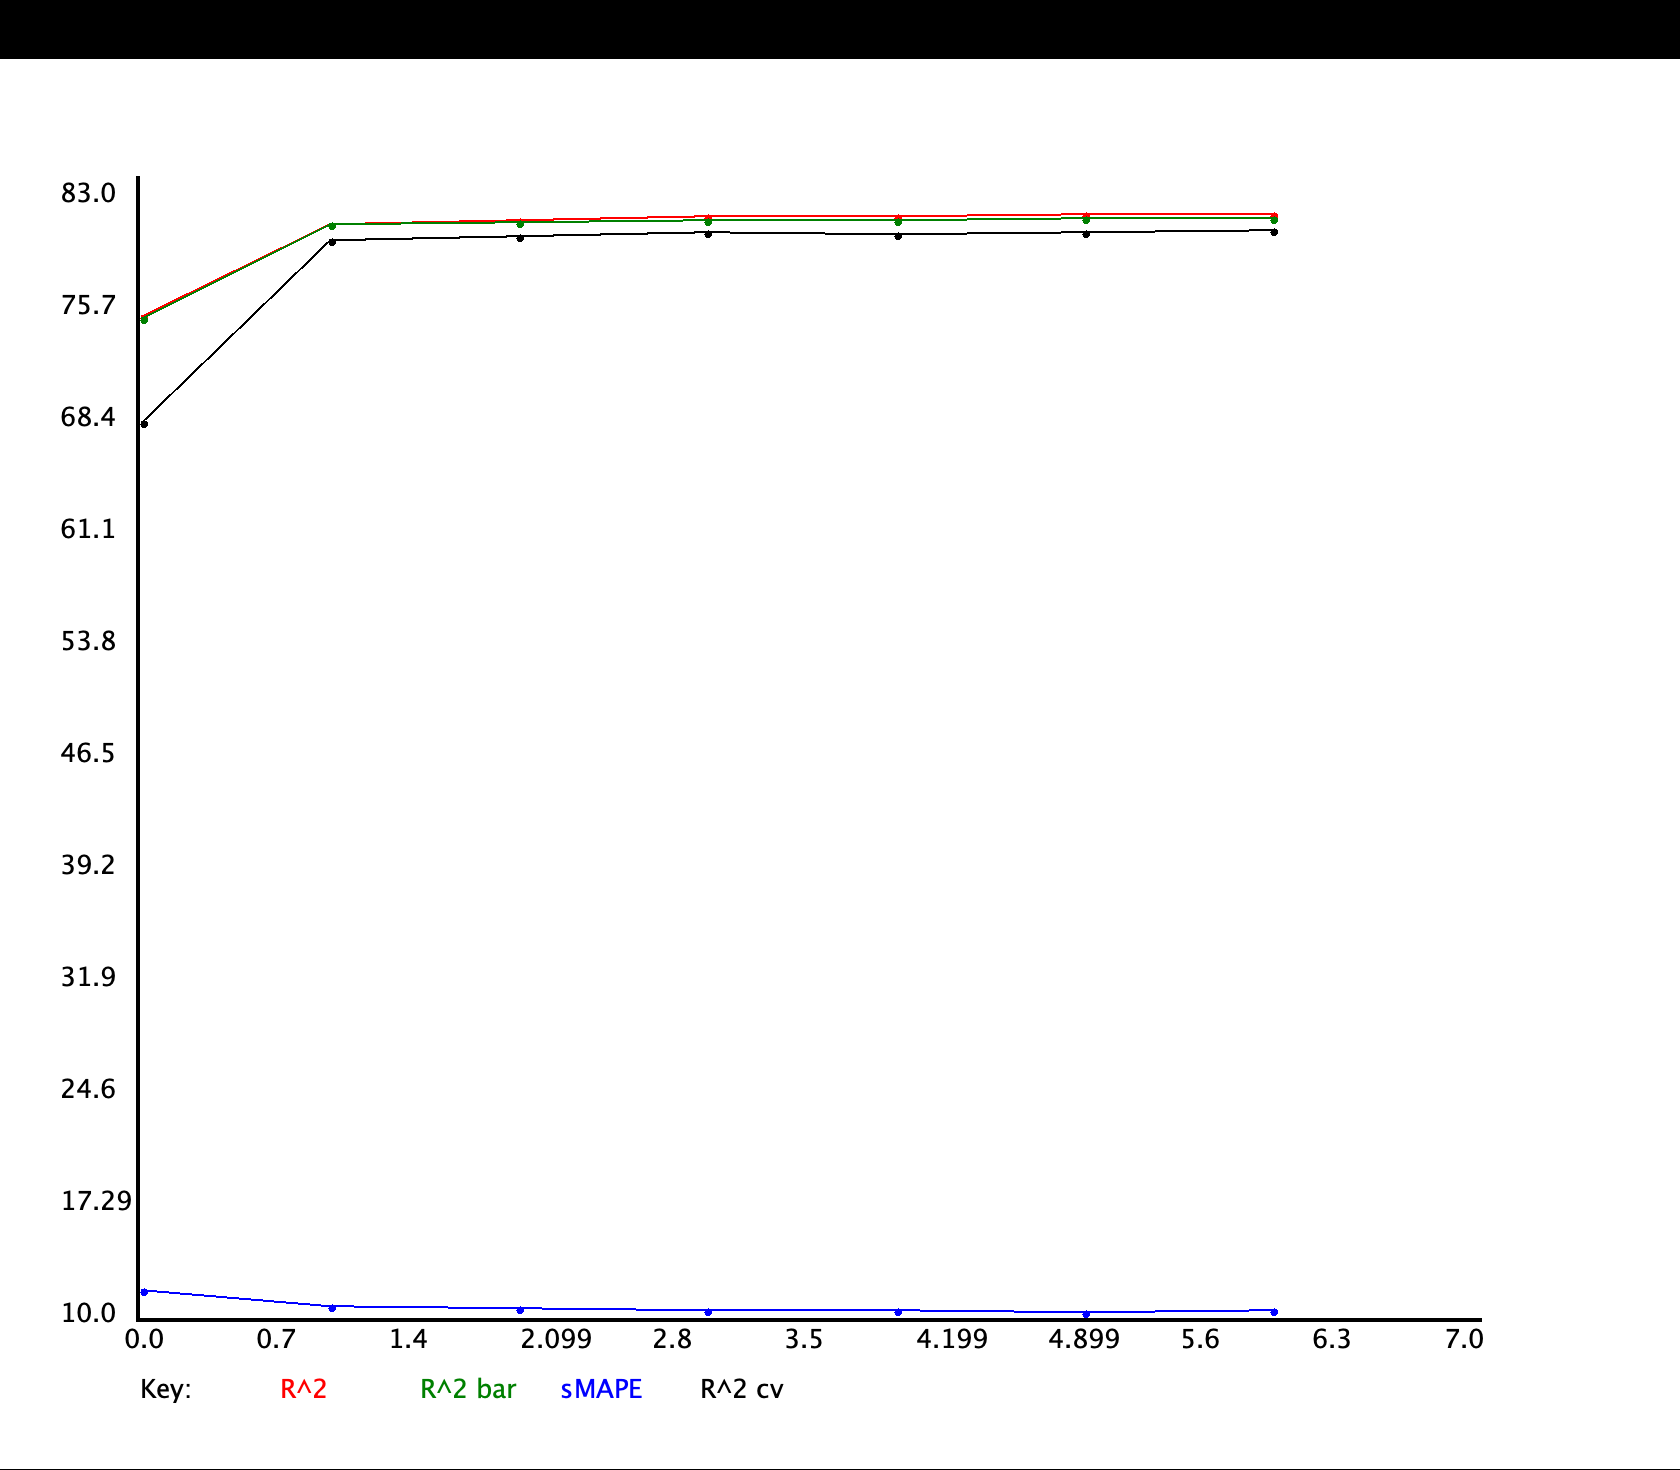
\includegraphics[width=\textwidth]{../Auto_MPG_Scalation_Plots/Scalation_Reg_rSq_Stepwise.png}
     \end{subfigure}
     \hfill
     \begin{subfigure}[b]{0.4\textwidth}
         \centering
         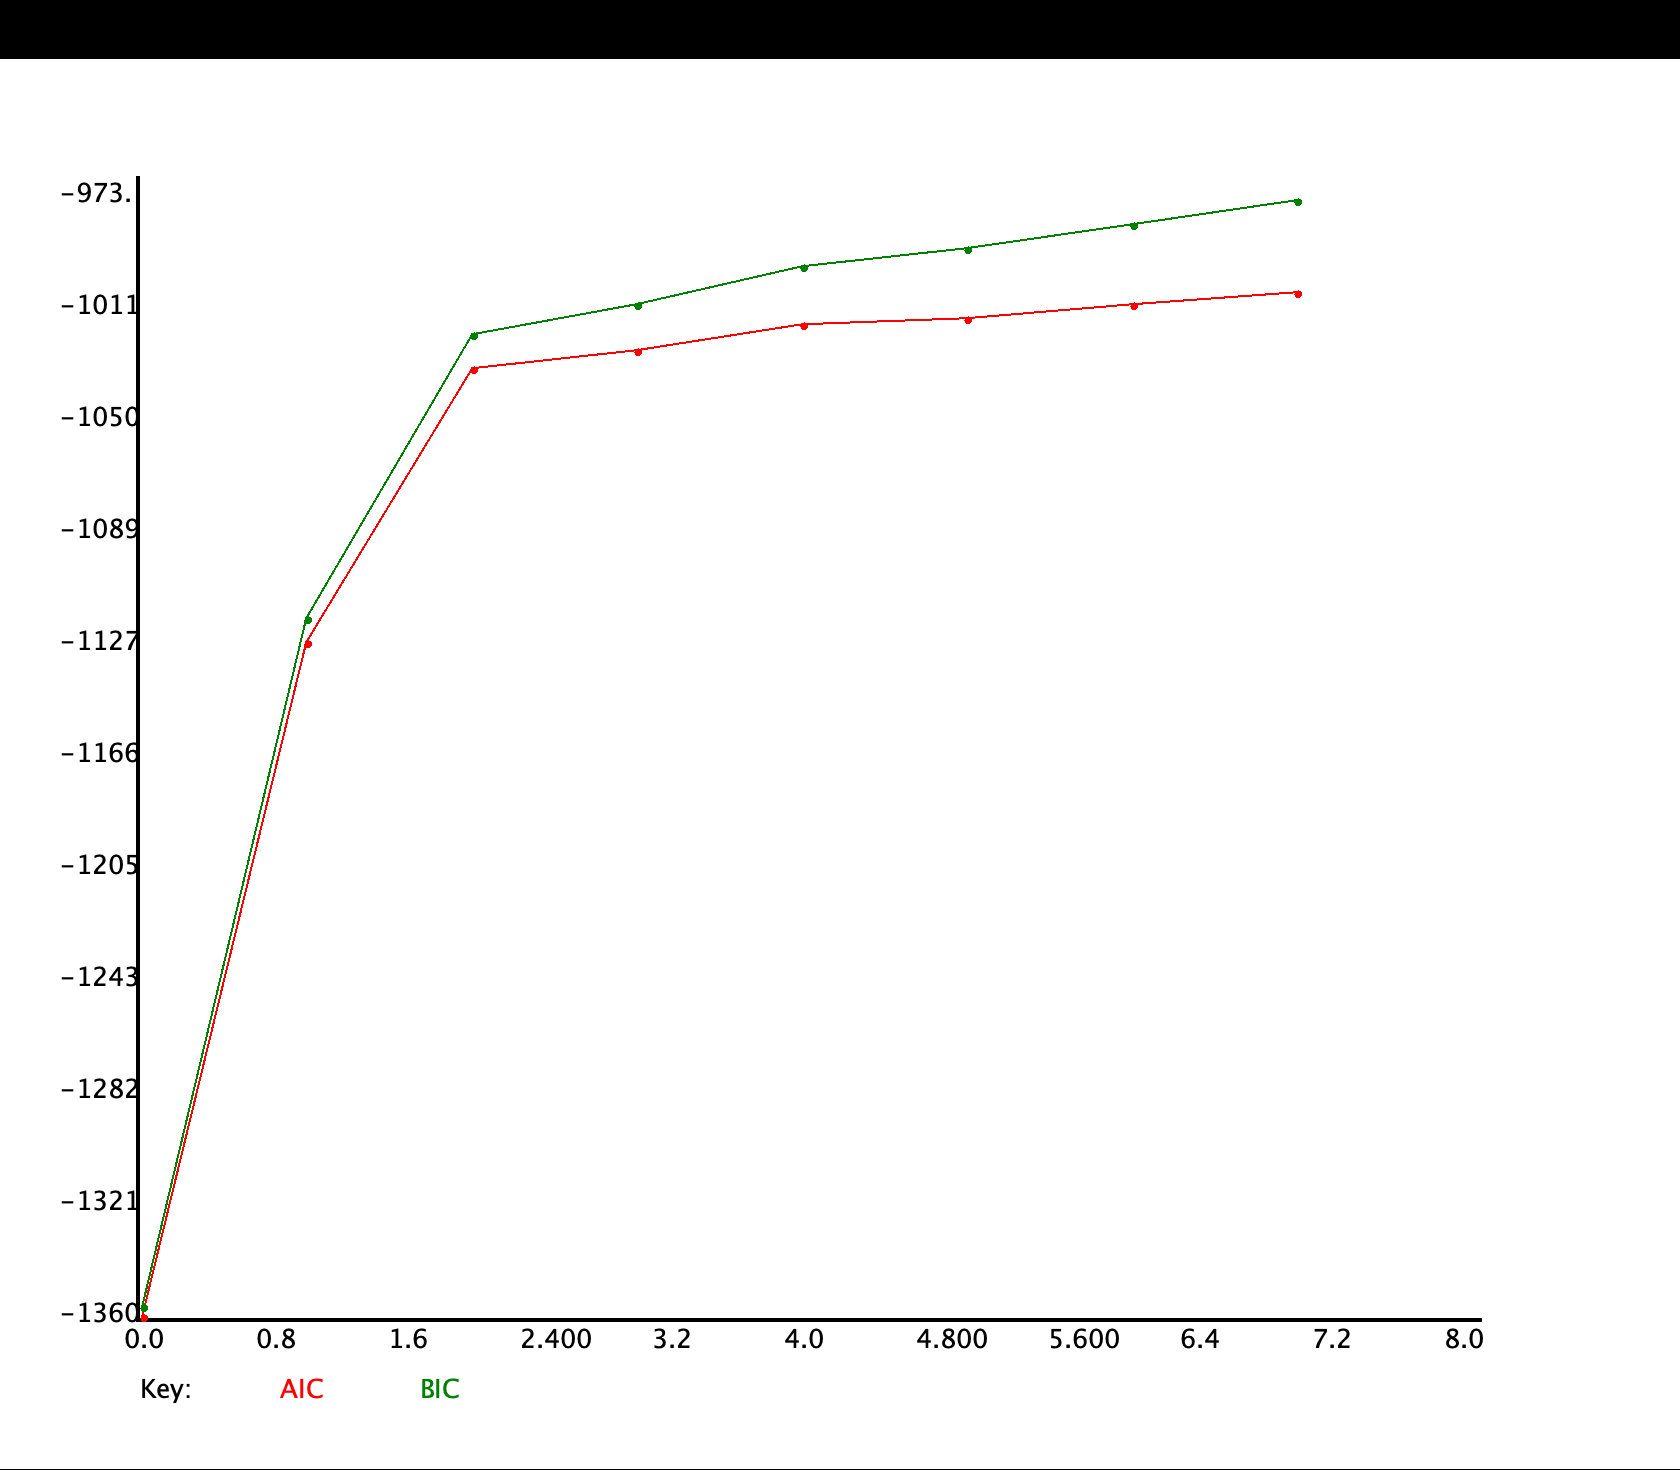
\includegraphics[width=\textwidth]{../Auto_MPG_Scalation_Plots/Scalation_Reg_AIC_BIC_Stepwise.png}
     \end{subfigure}

     \vspace{10pt} % Add some vertical spacing between rows

     % Second Row
     \begin{subfigure}[b]{0.49\textwidth}
         \centering
         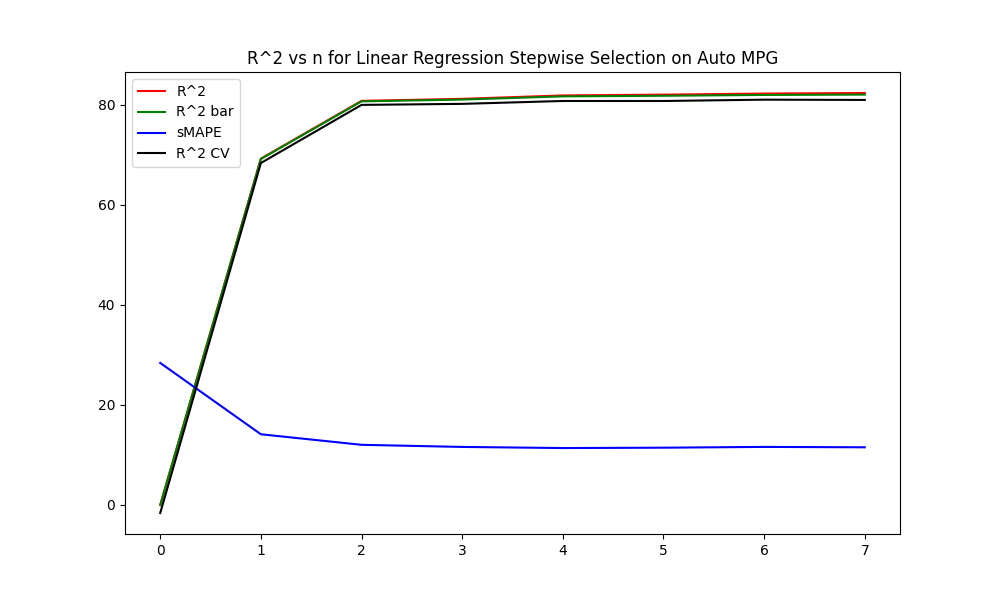
\includegraphics[width=\textwidth]{../Auto_MPG_Statsmodels_Plots/Statsmodels_Reg_rSq_Stepwise.png}
     \end{subfigure}
     \hfill
     \begin{subfigure}[b]{0.49\textwidth}
         \centering
         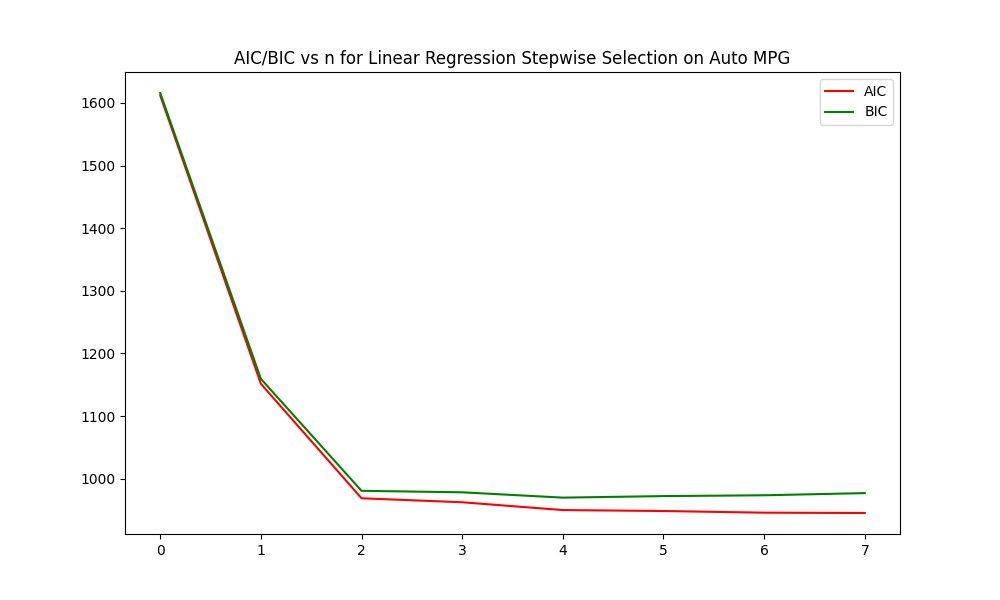
\includegraphics[width=\textwidth]{../Auto_MPG_Statsmodels_Plots/Statsmodels_Reg_AIC_BIC_Stepwise.png}
     \end{subfigure}
     
     \caption{Auto MPG Linear Regression Stepwise Selection Quality of Fit Metrics\\ Top Left: Scalation $R^2$, Top Right: Scalation AIC/BIC\\ Bottom Left: Statsmodels $R^2$, Bottom Right: Statsmodels AIC/BIC}
     \label{fig:Auto MPG Linear Regression Stepwise Selection Quality of Fit Metrics}
\end{figure}

\subsection{Ridge Regression}

\subsubsection{Quality of Fit}

Scalation Auto MPG Ridge Lambda Used: $0.01$

\noindent Statsmodels Auto MPG Ridge alpha Used: $0.0125$

\begin{figure}[H]
     \centering
     \captionsetup{justification=centering}
     % First Row
     \begin{subfigure}[b]{0.4\textwidth}
         \centering
         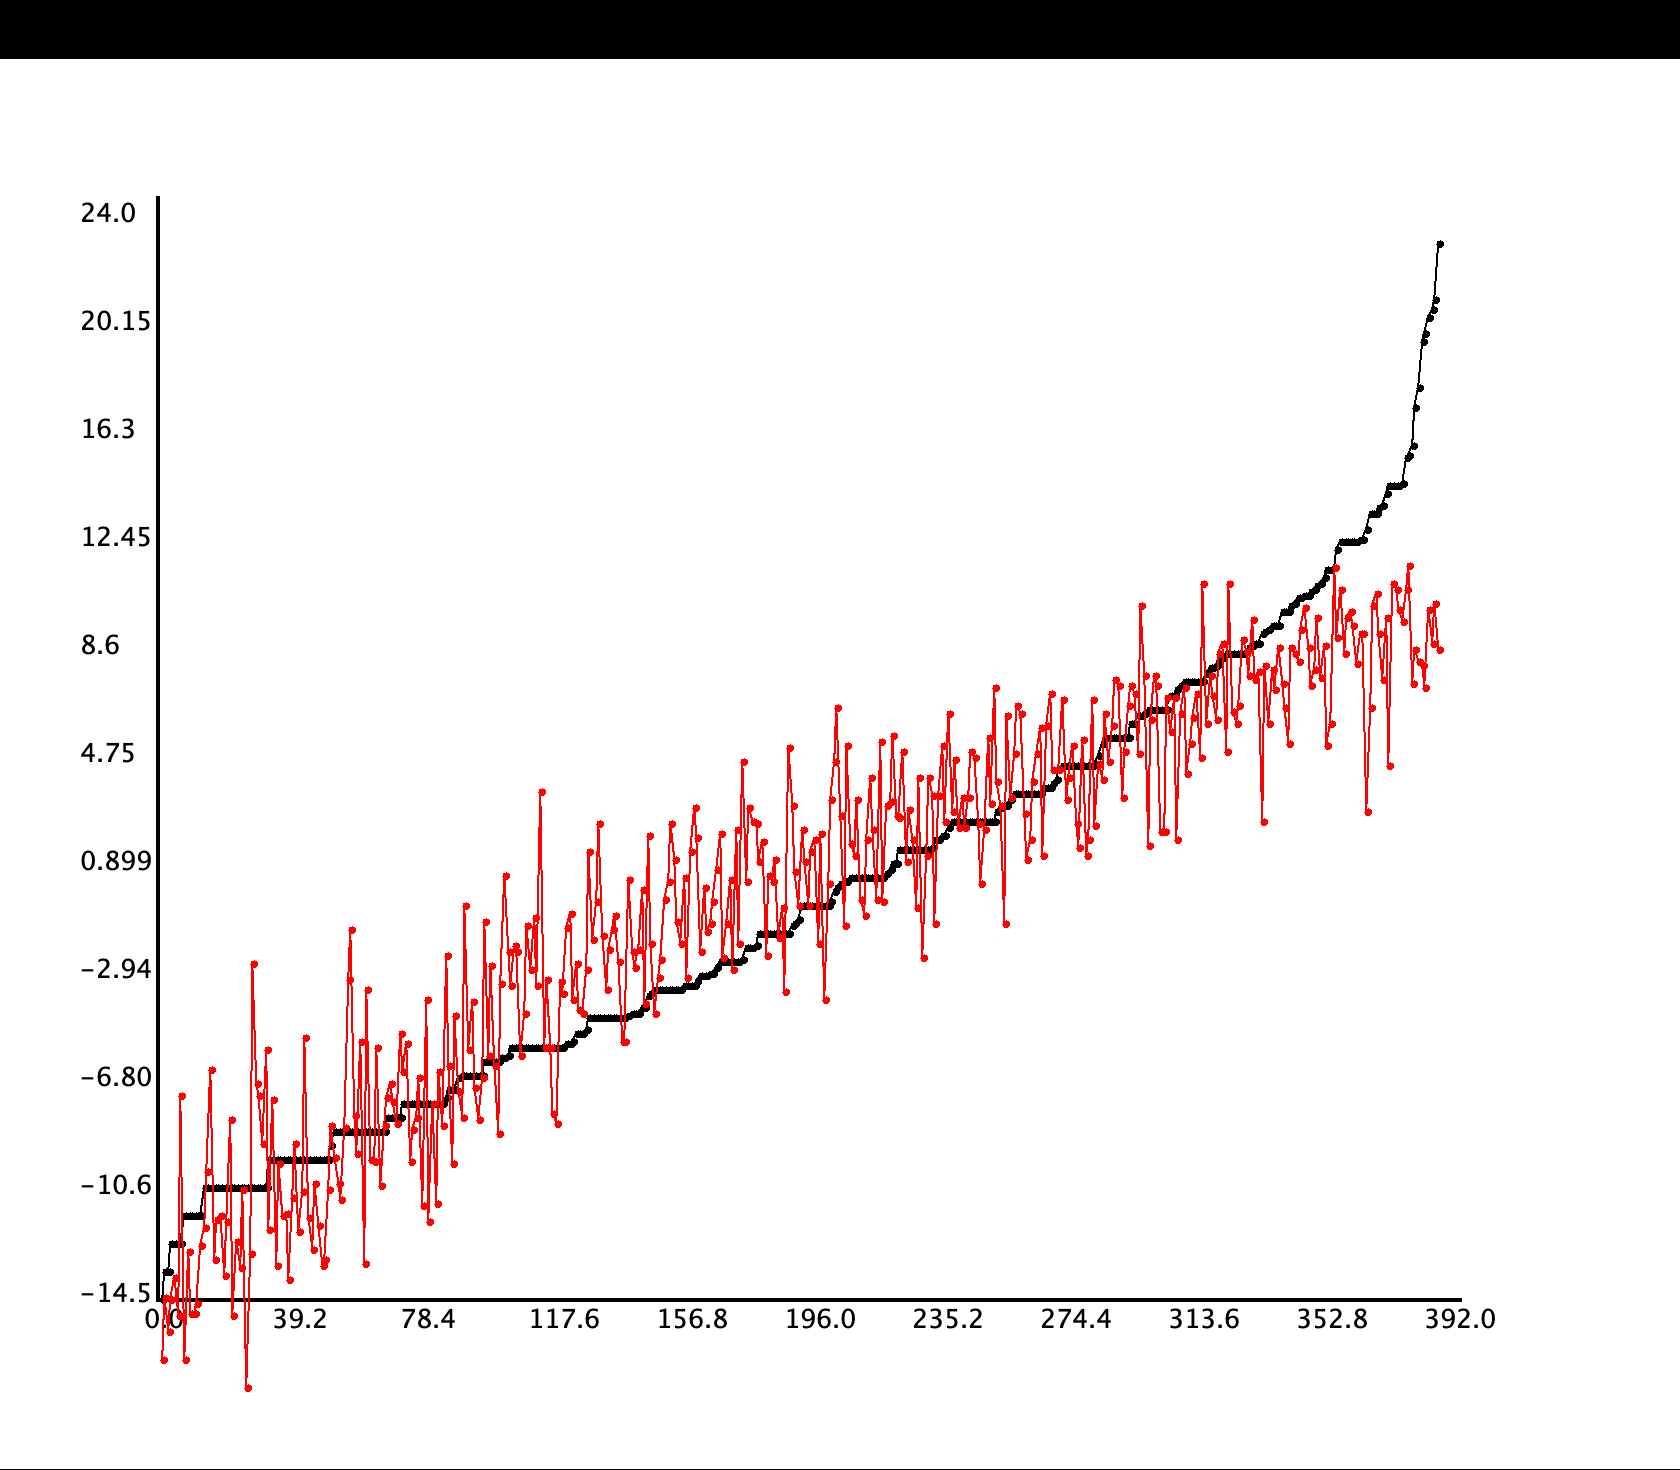
\includegraphics[width=\textwidth]{../Auto_MPG_Scalation_Plots/Scalation_Ridge_In_Sample.png}
     \end{subfigure}
     \hfill
     \begin{subfigure}[b]{0.4\textwidth}
         \centering
         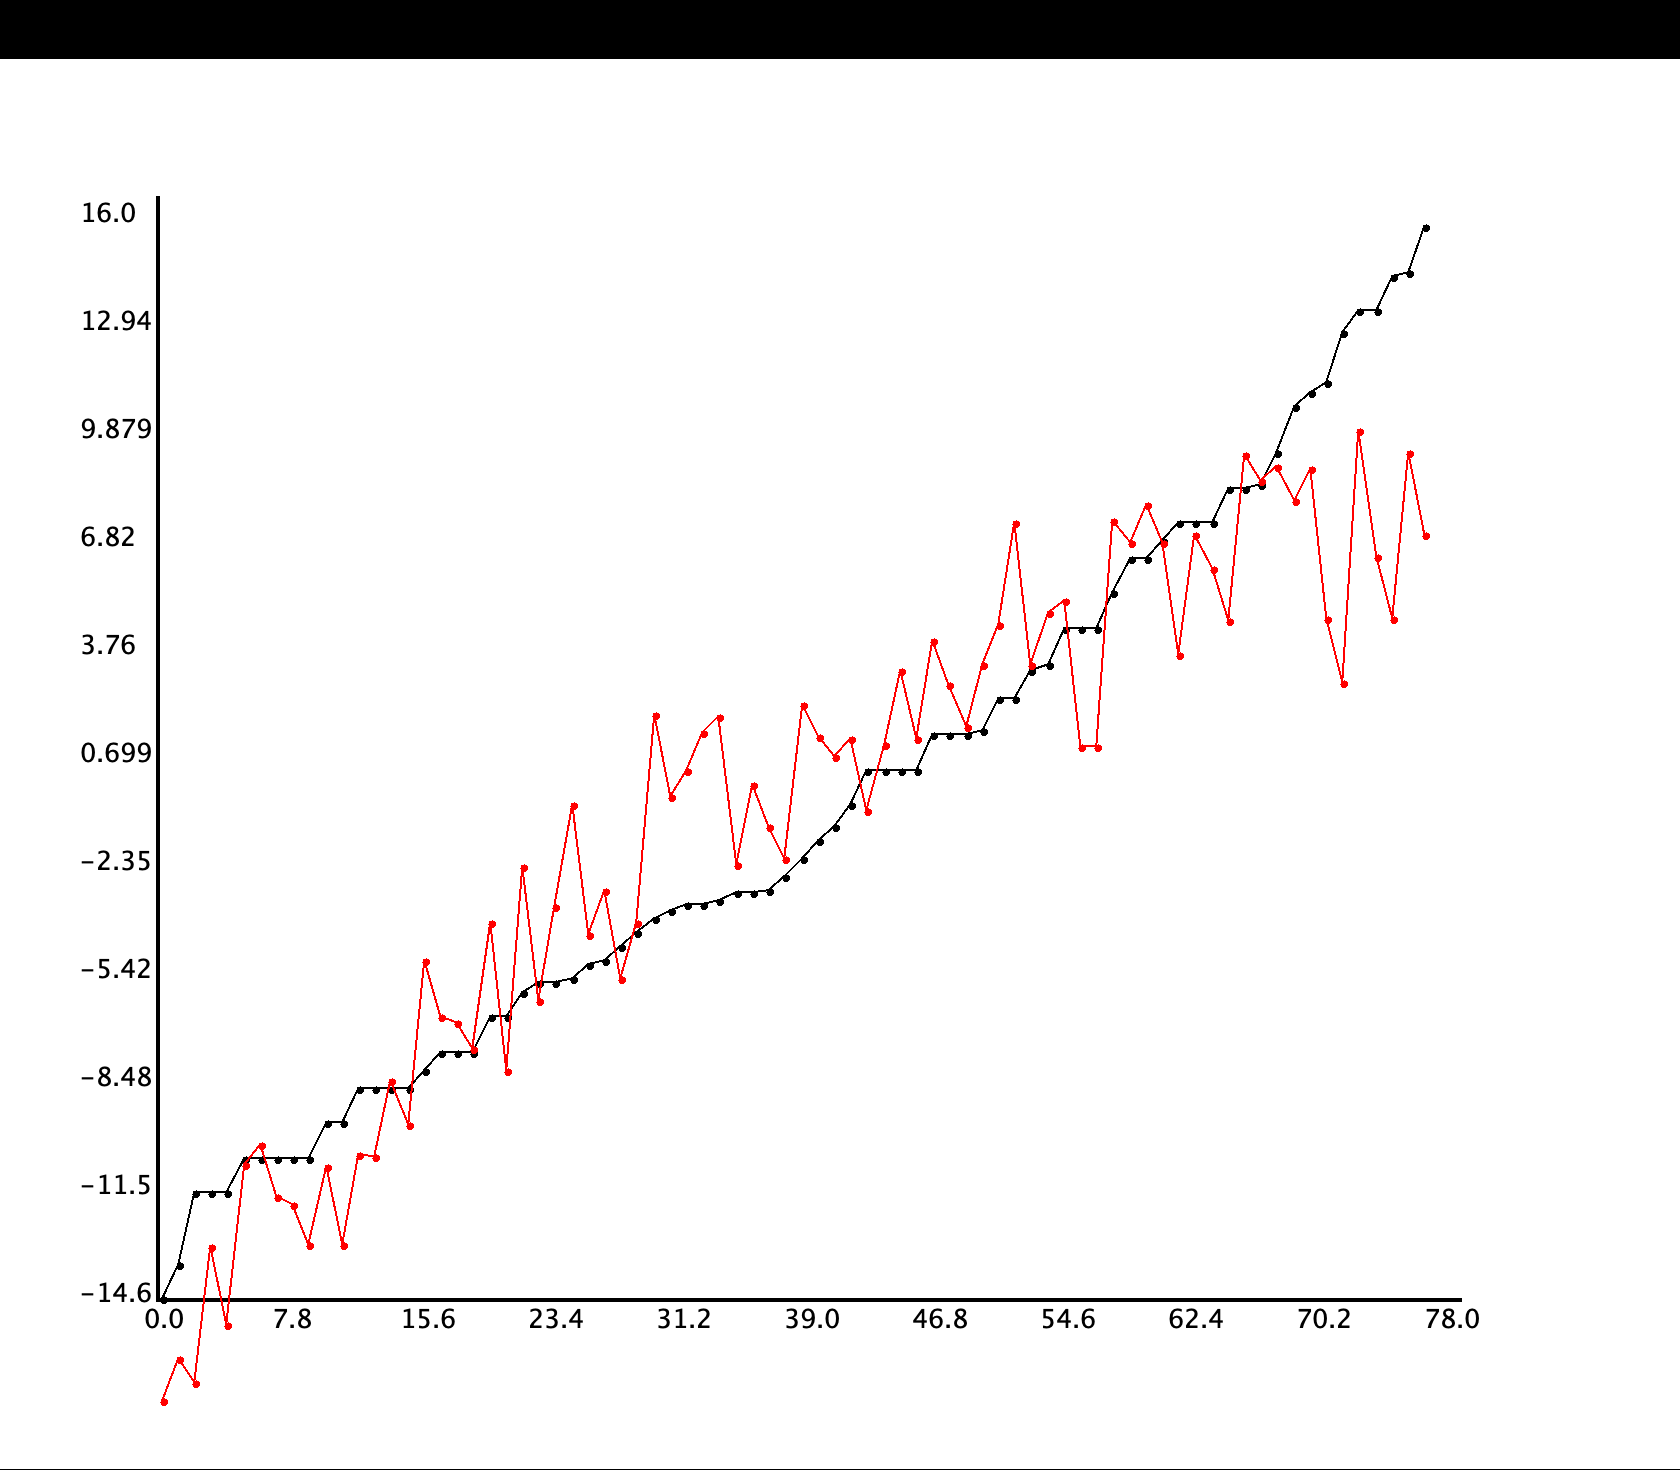
\includegraphics[width=\textwidth]{../Auto_MPG_Scalation_Plots/Scalation_Ridge_80_20.png}
     \end{subfigure}

     \vspace{10pt} % Add some vertical spacing between rows

     % Second Row
     \begin{subfigure}[b]{0.49\textwidth}
         \centering
         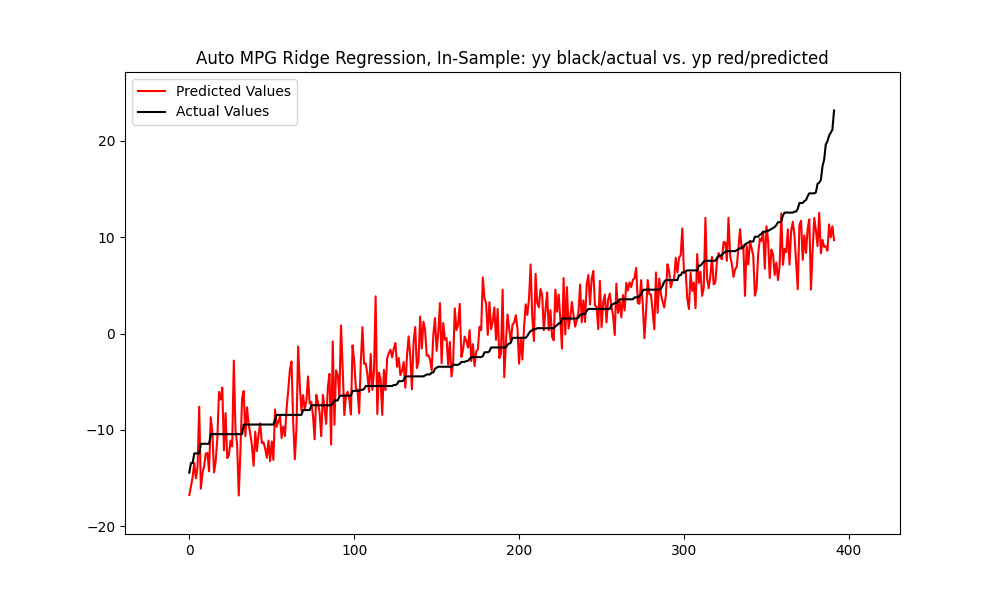
\includegraphics[width=\textwidth]{../Auto_MPG_Statsmodels_Plots/Statsmodels_Ridge_In_Sample.png}
     \end{subfigure}
     \hfill
     \begin{subfigure}[b]{0.49\textwidth}
         \centering
         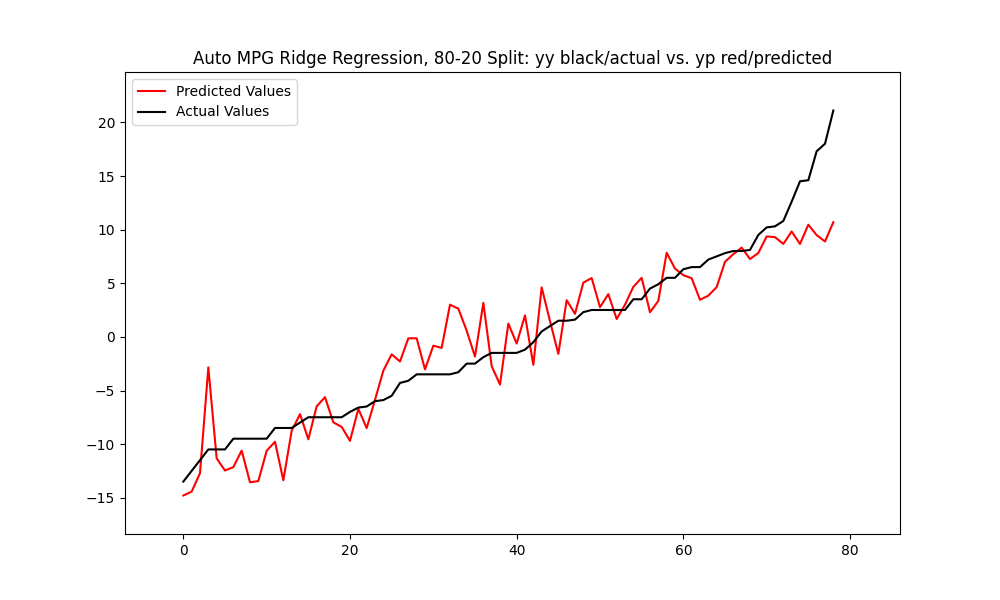
\includegraphics[width=\textwidth]{../Auto_MPG_Statsmodels_Plots/Statsmodels_Ridge_80_20.png}
     \end{subfigure}
     
     \caption{Auto MPG Ridge Regression Plots\\ Top Left: Scalation In-Sample, Top Right: Scalation Out-of-Sample\\ Bottom Left: Statsmodels In-Sample, Bottom Right: Statsmodels Out-of-Sample\\ black: actual y-values, red: predicted y-values}
     \label{fig:Auto MPG Ridge Regression Plots}
\end{figure}

\begin{table}[H]
\centering
\caption{Scalation - Auto MPG Ridge Regression}
\label{tab:Scalation - Auto MPG Ridge Regression}
\begin{tabular}{|c|c|c|} \hline 
Metric & In-Sample & 80-20 Split \\ \hline \hline 
rSq &0.808501 & 0.821456 \\ \hline 
rSqBar &0.804501 &      0.817726 \\ \hline 
sst &23819.0 &  4731.23 \\ \hline 
sse &4561.32 &  844.736 \\ \hline 
sde &3.41552 &  3.30307 \\ \hline 
mse0 &11.6360 & 10.8299 \\ \hline 
rmse &3.41116 & 3.29089 \\ \hline 
mae &2.61162 &  2.48838 \\ \hline 
smape &64.4083 &        63.9305 \\ \hline 
m &392.000 &    78.0000 \\ \hline 
dfr &8.00000 &  8.00000 \\ \hline 
df &383.000 &   383.000 \\ \hline 
fStat &202.126 &        220.265 \\ \hline 
aic &-1019.23 & -185.588 \\ \hline 
bic &-983.487 & -164.378 \\ \hline 
\end{tabular}
\end{table}

\begin{table}[H]
\centering
\caption{Statsmodels - Auto MPG Ridge Regression}
\label{tab:Statsmodels - Auto MPG Ridge Regression}
\begin{tabular}{|c|c|c|}\hline
Metric & In-Sample & 80-20 Split \\ \hline \hline
rSq & 0.8230 & 0.8384 \\ \hline
rSqBar & 0.8198 & 0.8224 \\ \hline
sst & 23818.9935 & 4910.2699 \\ \hline
sse & 4215.8423 & 793.6373 \\ \hline
sde & 3.3134 & 3.3434 \\ \hline
mse0 & 10.7547 & 10.0460 \\ \hline
rmse & 3.2794 & 3.1695 \\ \hline
mae & 2.4901 & 2.4065 \\ \hline
smape & 61.4391 & 57.5645 \\ \hline
m & 392.0000 & 79.0000 \\ \hline
dfr & 8.0000 & 8.0000 \\ \hline
df & 384.0000 & 71.0000 \\ \hline
fStat & 223.1941 & 46.0350 \\ \hline
aic & 947.1344 & 198.2671 \\ \hline
bic & 978.9045 & 217.2227 \\ \hline
\end{tabular}
\end{table}

\begin{table}[H]
\centering
\caption{Scalation - Auto MPG Ridge Regression CV}
\label{tab:Scalation - Auto MPG Ridge Regression CV}
\begin{tabular}{|c|c|c|c|c|c|}\hline
Metric & num folds & min & max & mean & stdev \\ \hline \hline
rSq & 5 & 0.786 & 0.821 & 0.797 & 0.014 \\ \hline
rSqBar & 5 & 0.781 & 0.818 & 0.793 & 0.015 \\ \hline
sst & 5 & 3962.818 & 5671.580 & 4700.481 & 620.767 \\ \hline
sse & 5 & 822.721 & 1201.114 & 955.120 & 153.547 \\ \hline
sde & 5 & 3.174 & 3.776 & 3.439 & 0.244 \\ \hline
mse0 & 5 & 10.548 & 15.399 & 12.245 & 1.969 \\ \hline
rmse & 5 & 3.248 & 3.924 & 3.491 & 0.274 \\ \hline
mae & 5 & 2.488 & 2.822 & 2.681 & 0.143 \\ \hline
smape & 5 & 61.709 & 71.709 & 66.453 & 4.637 \\ \hline
m & 5 & 78.000 & 78.000 & 78.000 & 0.000 \\ \hline
dfr & 5 & 8.000 & 8.000 & 8.000 & 0.000 \\ \hline
df & 5 & 383.000 & 383.000 & 383.000 & 0.000 \\ \hline
fStat & 5 & 175.717 & 220.242 & 188.950 & 18.097 \\ \hline
aic & 5 & -202.131 & -184.566 & -190.712 & 7.128 \\ \hline
bic & 5 & -180.920 & -163.356 & -169.502 & 7.128 \\ \hline
\end{tabular}
\end{table}

\begin{table}[H]
\centering
\caption{Statsmodels - Auto MPG Ridge Regression CV}
\label{tab:Statsmodels - Auto MPG Ridge Regression CV}
\begin{tabular}{|c|c|c|c|c|c|}\hline
Metric & num folds & min & max & mean & stdev \\ \hline \hline
rSq & 5 & 0.7420 & 0.8418 & 0.8101 & 0.0361 \\ \hline
rSqBar & 5 & 0.7162 & 0.8259 & 0.7912 & 0.0397 \\ \hline
sst & 5 & 3880.9704 & 5093.9237 & 4721.1782 & 441.3031 \\ \hline
sse & 5 & 790.9033 & 1001.1262 & 881.2419 & 77.4845 \\ \hline
sde & 5 & 3.3376 & 3.7818 & 3.5349 & 0.1610 \\ \hline
mse0 & 5 & 10.0114 & 12.8350 & 11.2436 & 1.0240 \\ \hline
rmse & 5 & 3.1641 & 3.5826 & 3.3497 & 0.1519 \\ \hline
mae & 5 & 2.3684 & 2.9441 & 2.5567 & 0.2084 \\ \hline
smape & 5 & 56.1954 & 73.4893 & 62.6259 & 6.7820 \\ \hline
m & 5 & 78.0000 & 79.0000 & 78.4000 & 0.4899 \\ \hline
dfr & 5 & 8.0000 & 8.0000 & 8.0000 & 0.0000 \\ \hline
df & 5 & 70.0000 & 71.0000 & 70.4000 & 0.4899 \\ \hline
fStat & 5 & 25.1703 & 46.5448 & 39.0075 & 7.7583 \\ \hline
aic & 5 & 197.9945 & 215.0694 & 205.3684 & 6.5463 \\ \hline
bic & 5 & 216.9501 & 233.9231 & 224.2628 & 6.5280 \\ \hline
\end{tabular}
\end{table}

\subsubsection{Feature Selection}

Scalation Forward Selection: displacement, weight, origin 2, modelyear, cylinders, acceleration, horsepower, origin 3

Statsmodels Forward Selection: Null, weight, model year, origin 3, origin 2, displacement, horsepower, cylinders, acceleration

\begin{figure}[H]
     \centering
     \captionsetup{justification=centering}
     % First Row
     \begin{subfigure}[b]{0.4\textwidth}
         \centering
         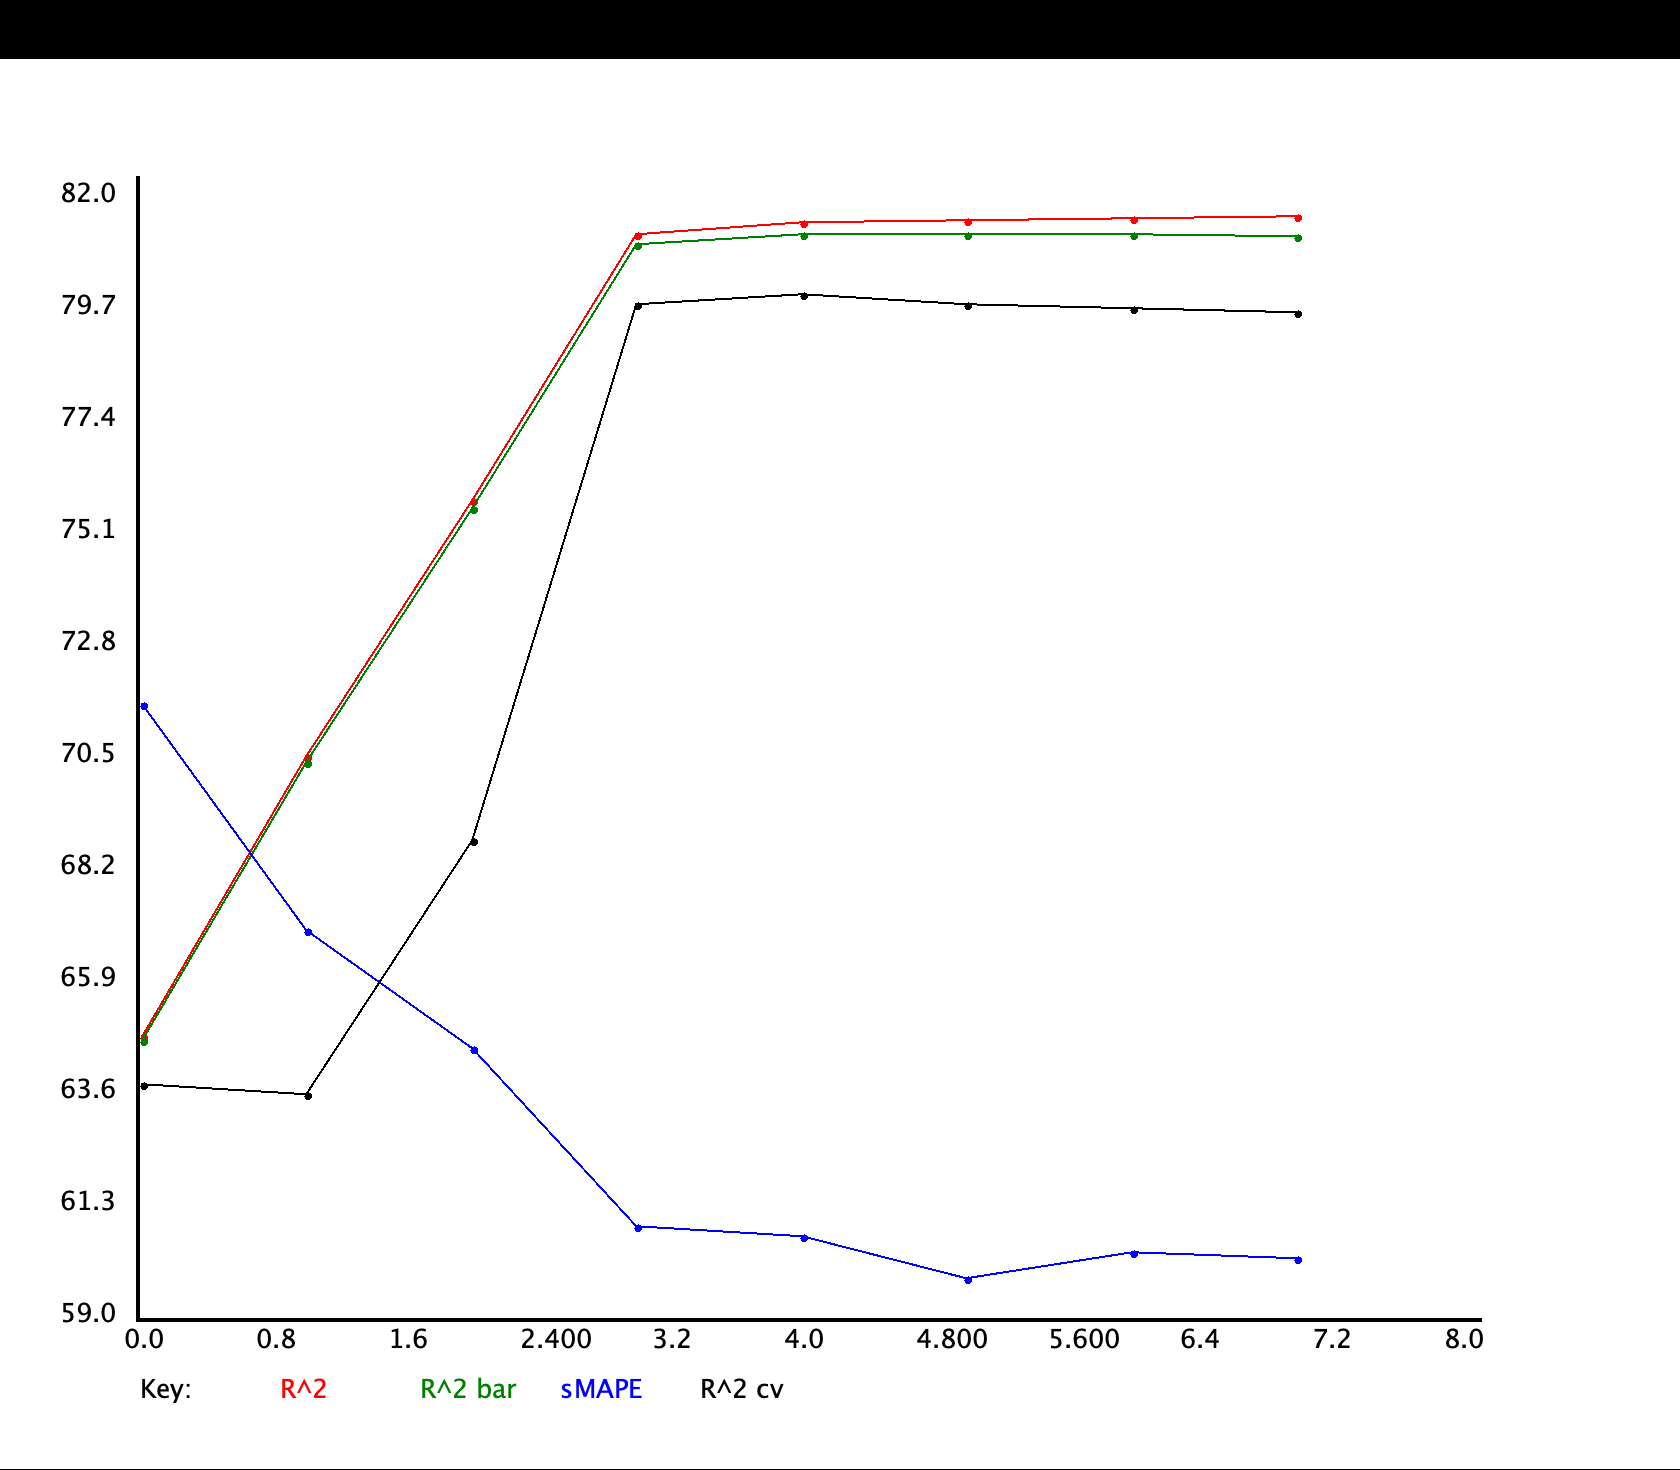
\includegraphics[width=\textwidth]{../Auto_MPG_Scalation_Plots/Scalation_Ridge_rSq_Forward.png}
     \end{subfigure}
     \hfill
     \begin{subfigure}[b]{0.4\textwidth}
         \centering
         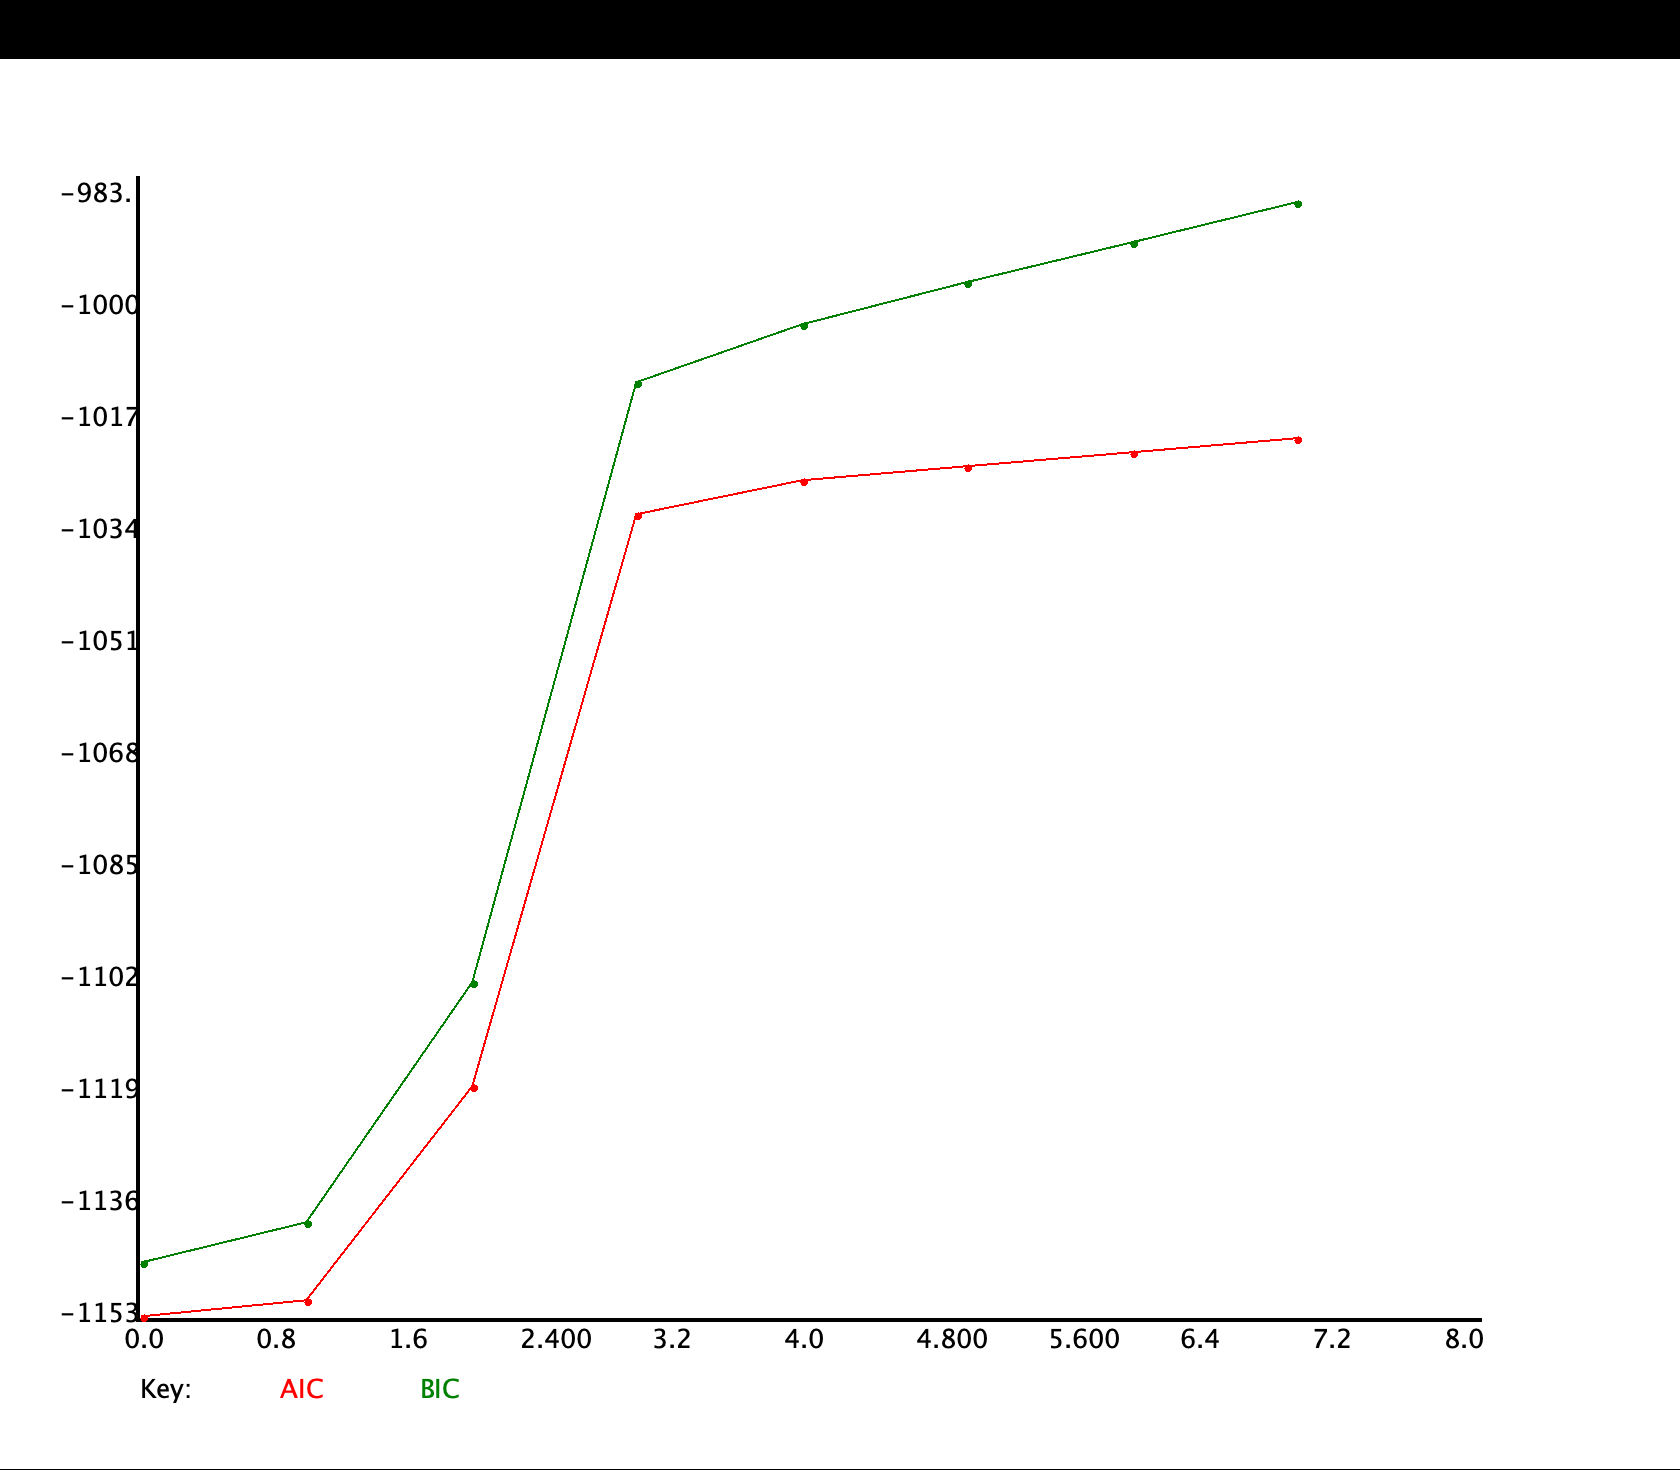
\includegraphics[width=\textwidth]{../Auto_MPG_Scalation_Plots/Scalation_Ridge_AIC_BIC_Forward.png}
     \end{subfigure}

     \vspace{10pt} % Add some vertical spacing between rows

     % Second Row
     \begin{subfigure}[b]{0.49\textwidth}
         \centering
         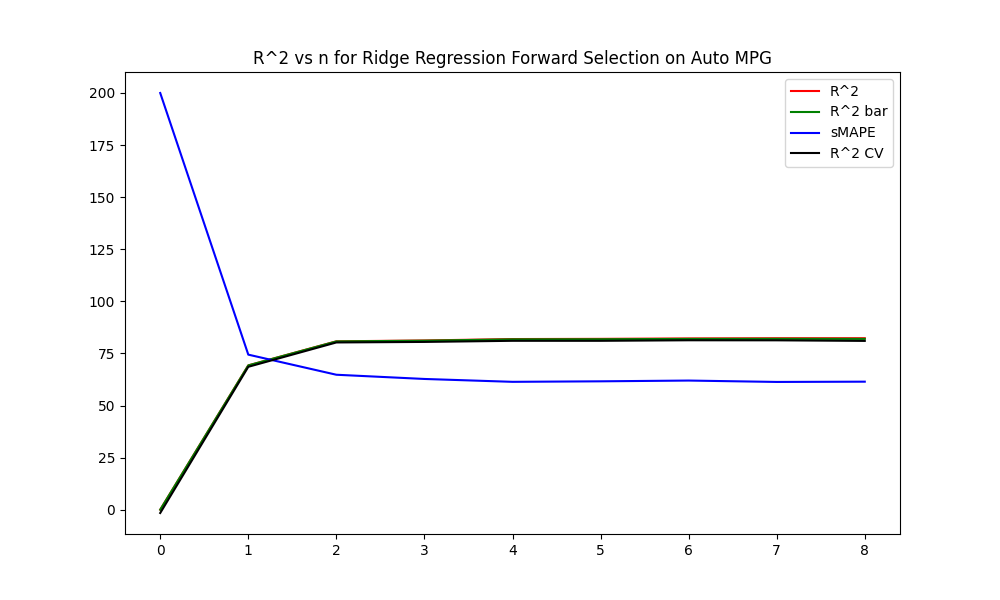
\includegraphics[width=\textwidth]{../Auto_MPG_Statsmodels_Plots/Statsmodels_Ridge_rSq_Forward.png}
     \end{subfigure}
     \hfill
     \begin{subfigure}[b]{0.49\textwidth}
         \centering
         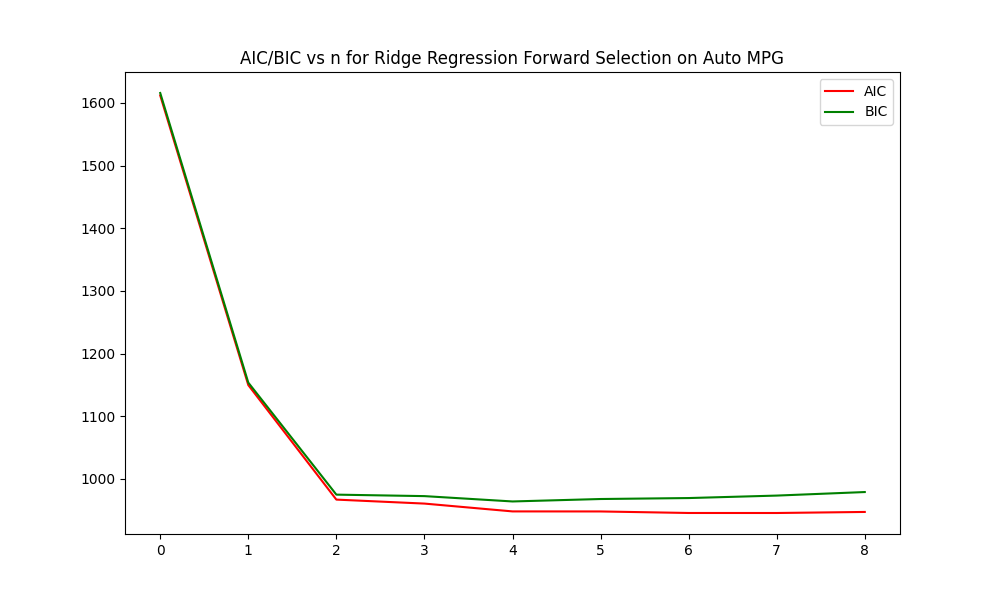
\includegraphics[width=\textwidth]{../Auto_MPG_Statsmodels_Plots/Statsmodels_Ridge_AIC_BIC_Forward.png}
     \end{subfigure}
     
     \caption{Auto MPG Ridge Regression Forward Selection Quality of Fit Metrics\\ Top Left: Scalation $R^2$, Top Right: Scalation AIC/BIC\\ Bottom Left: Statsmodels $R^2$, Bottom Right: Statsmodels AIC/BIC}
     \label{fig:Auto MPG Ridge Regression Forward Selection Quality of Fit Metrics}
\end{figure}

Scalation Backward Elimination Reversed: displacement, weight, cylinders, modelyear, acceleration, horsepower, origin 3, origin 2

Statsmodels Backward Elimination Reversed: Null, weight, model year, origin 3, origin 2, displacement, horsepower, cylinders, acceleration

\begin{figure}[H]
     \centering
     \captionsetup{justification=centering}
     % First Row
     \begin{subfigure}[b]{0.4\textwidth}
         \centering
         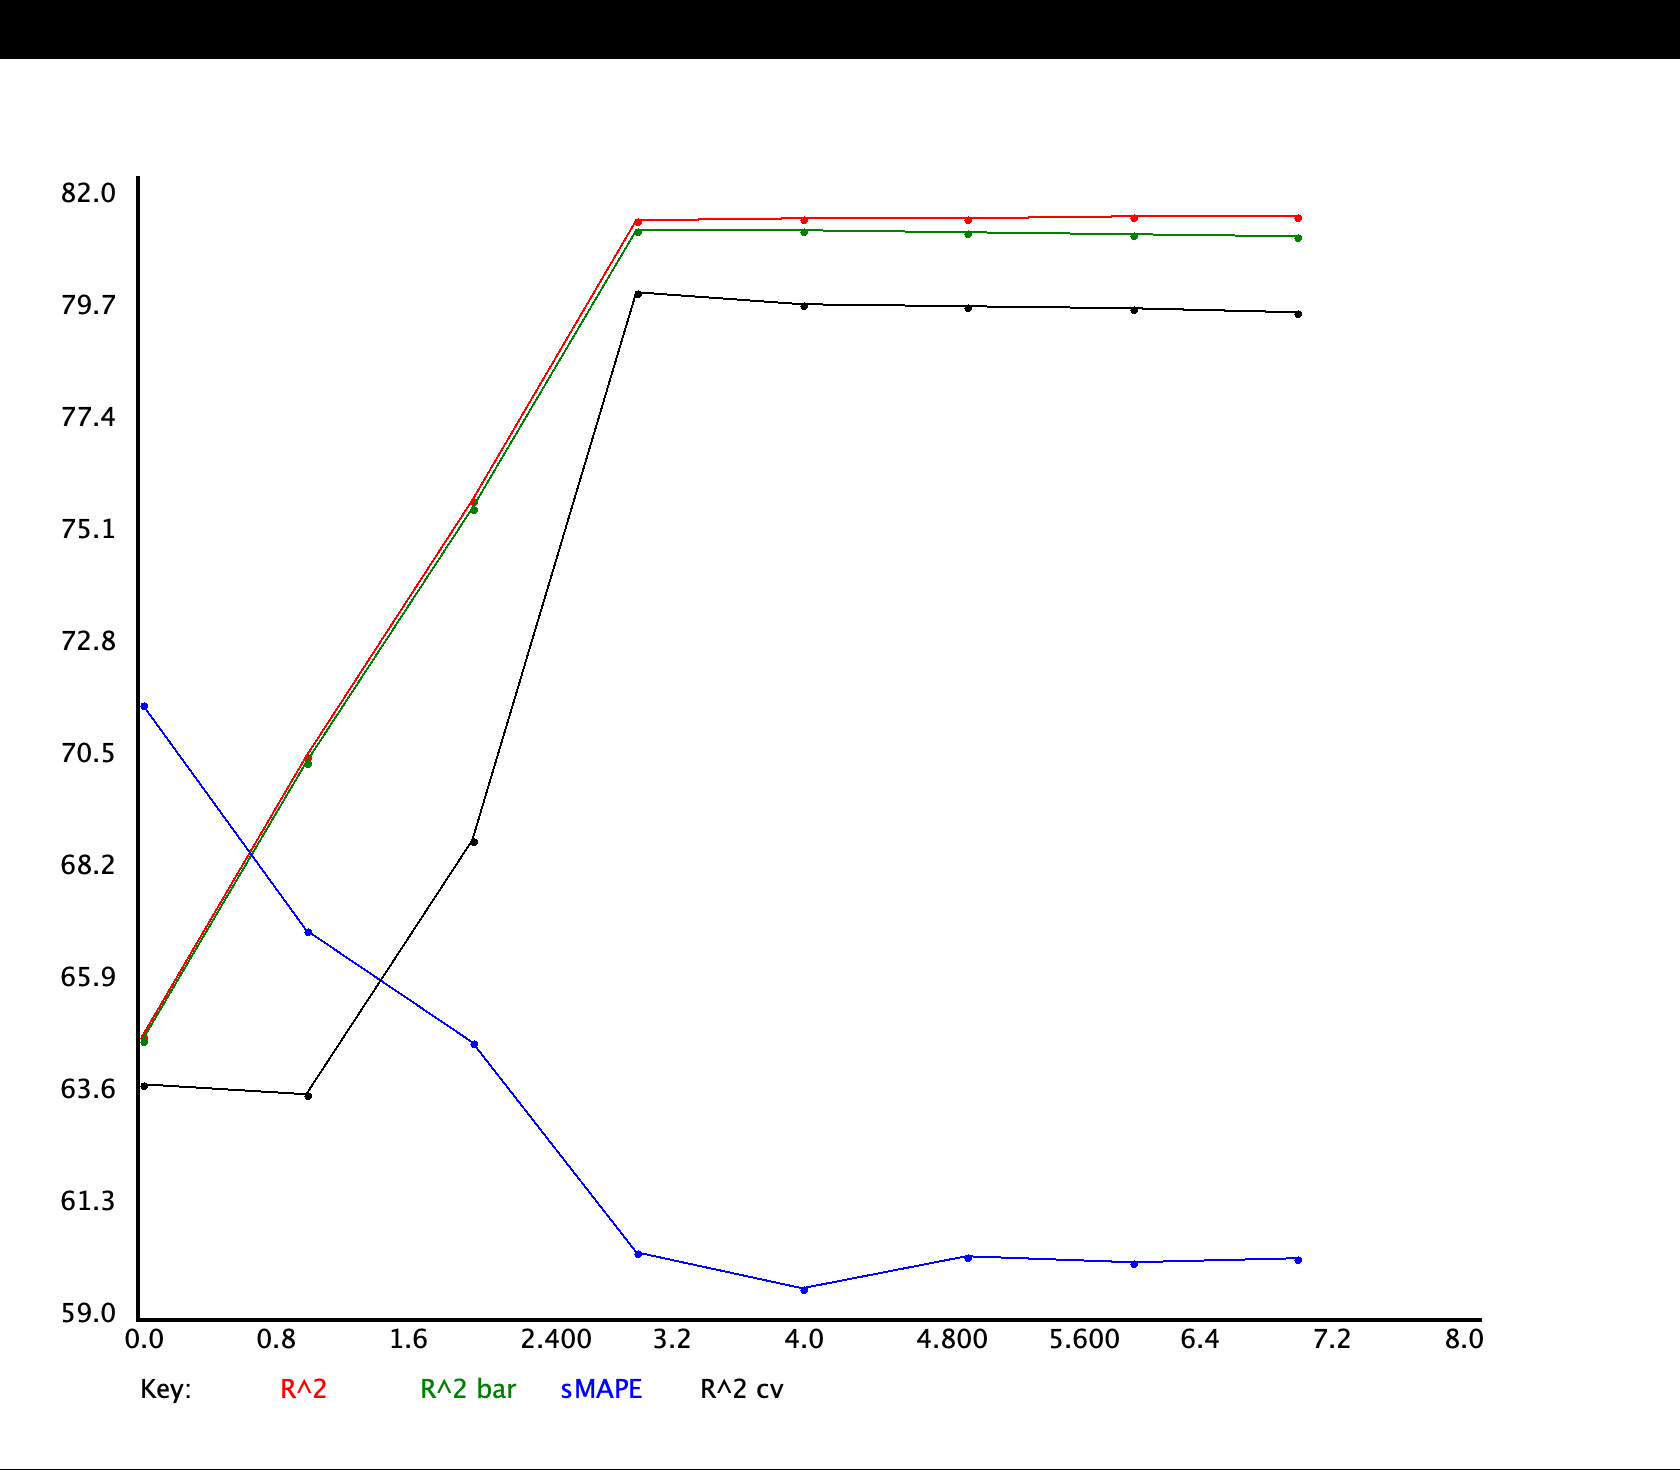
\includegraphics[width=\textwidth]{../Auto_MPG_Scalation_Plots/Scalation_Ridge_rSq_Backward.png}
     \end{subfigure}
     \hfill
     \begin{subfigure}[b]{0.4\textwidth}
         \centering
         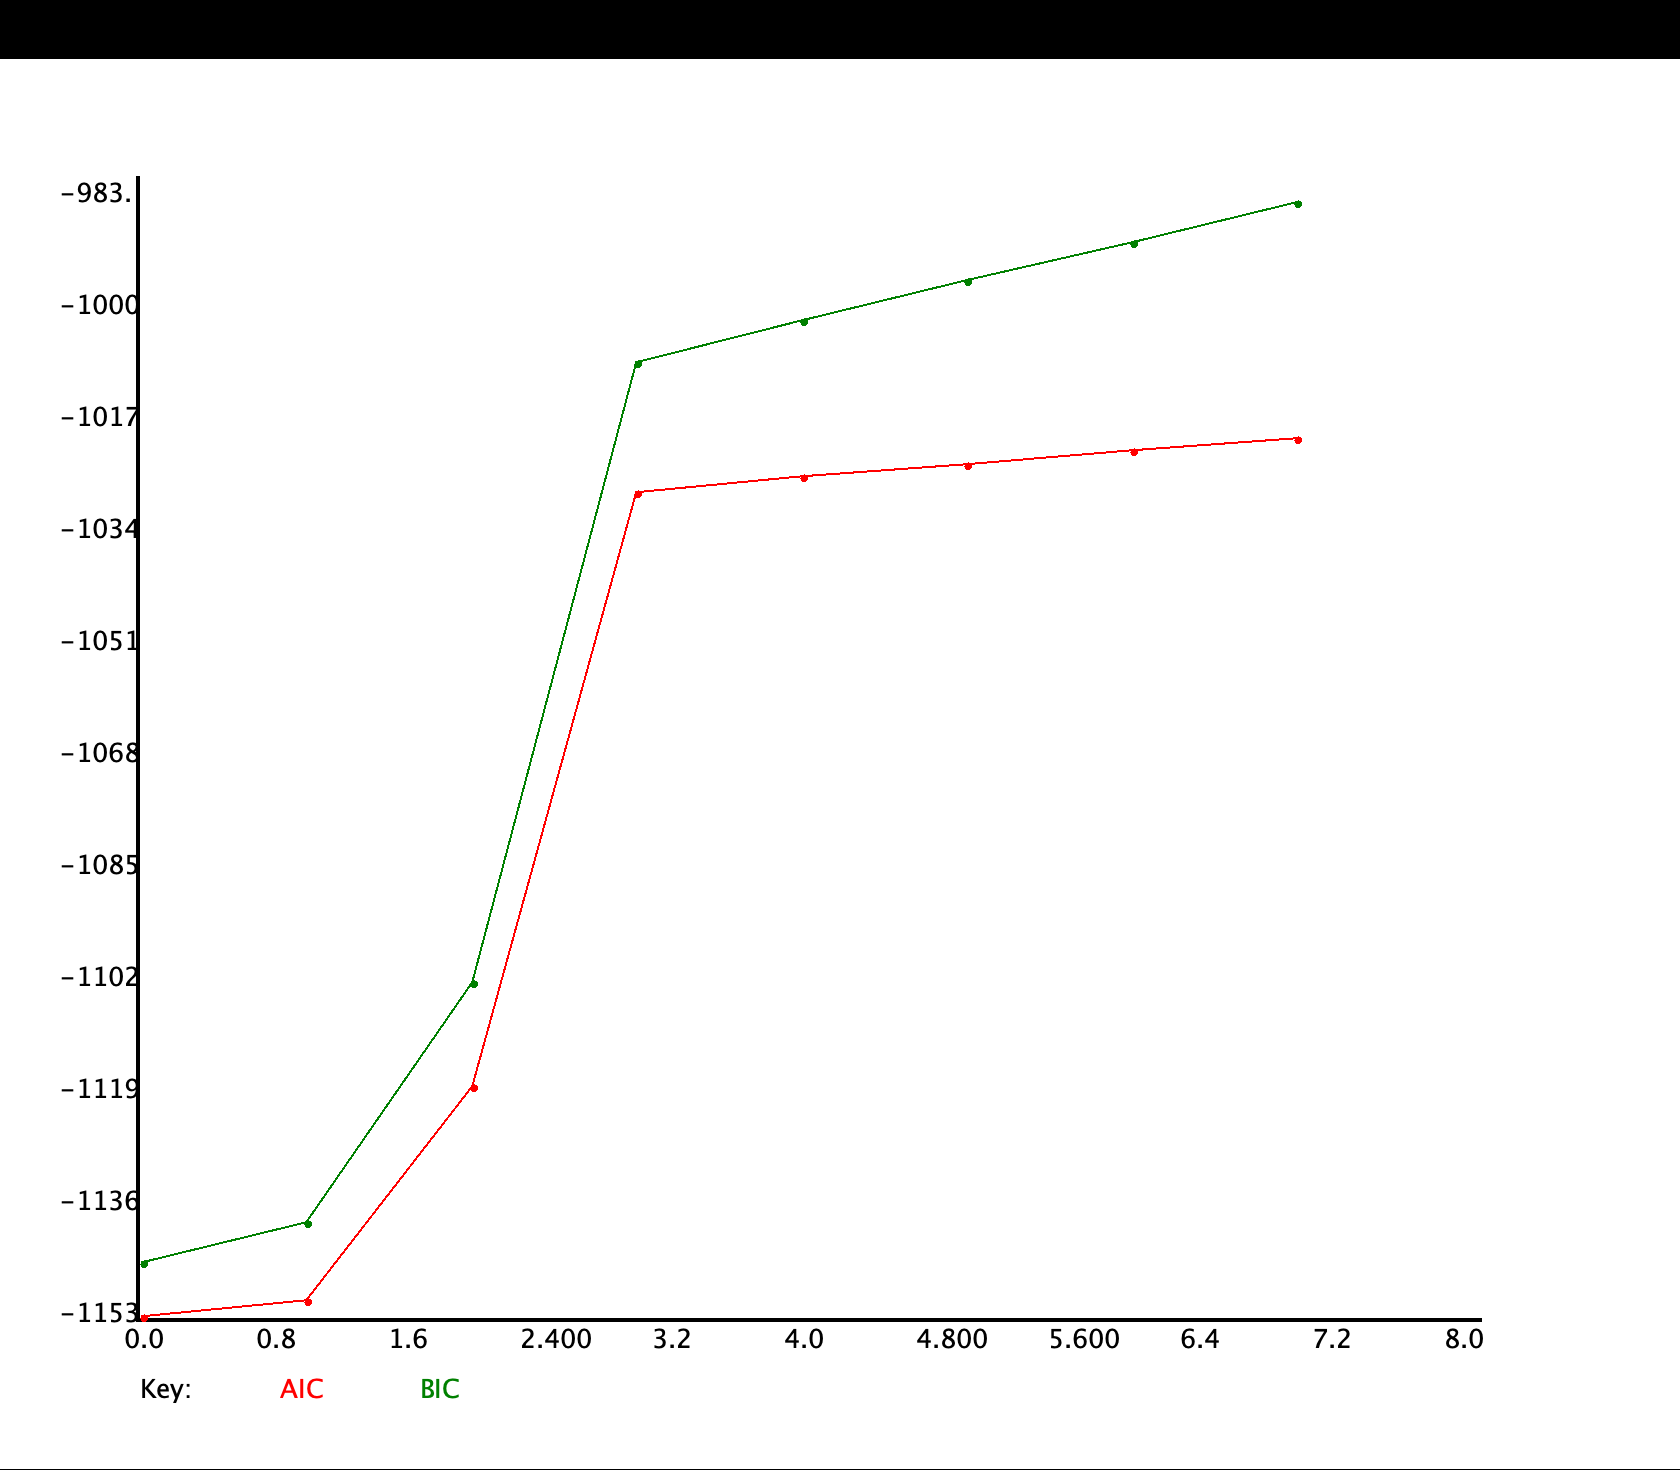
\includegraphics[width=\textwidth]{../Auto_MPG_Scalation_Plots/Scalation_Ridge_AIC_BIC_Backward.png}
     \end{subfigure}

     \vspace{10pt} % Add some vertical spacing between rows

     % Second Row
     \begin{subfigure}[b]{0.49\textwidth}
         \centering
         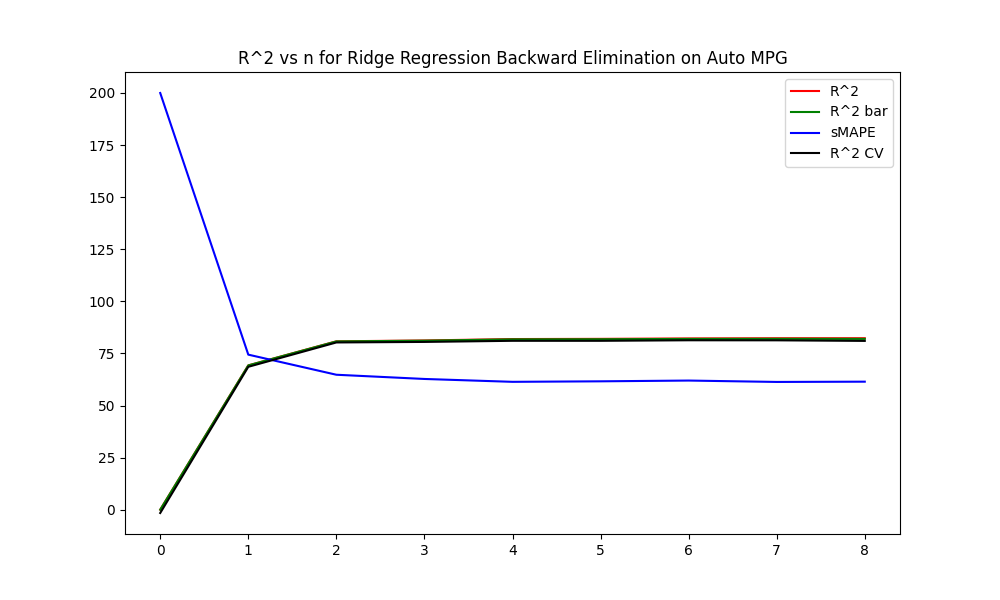
\includegraphics[width=\textwidth]{../Auto_MPG_Statsmodels_Plots/Statsmodels_Ridge_rSq_Backward.png}
     \end{subfigure}
     \hfill
     \begin{subfigure}[b]{0.49\textwidth}
         \centering
         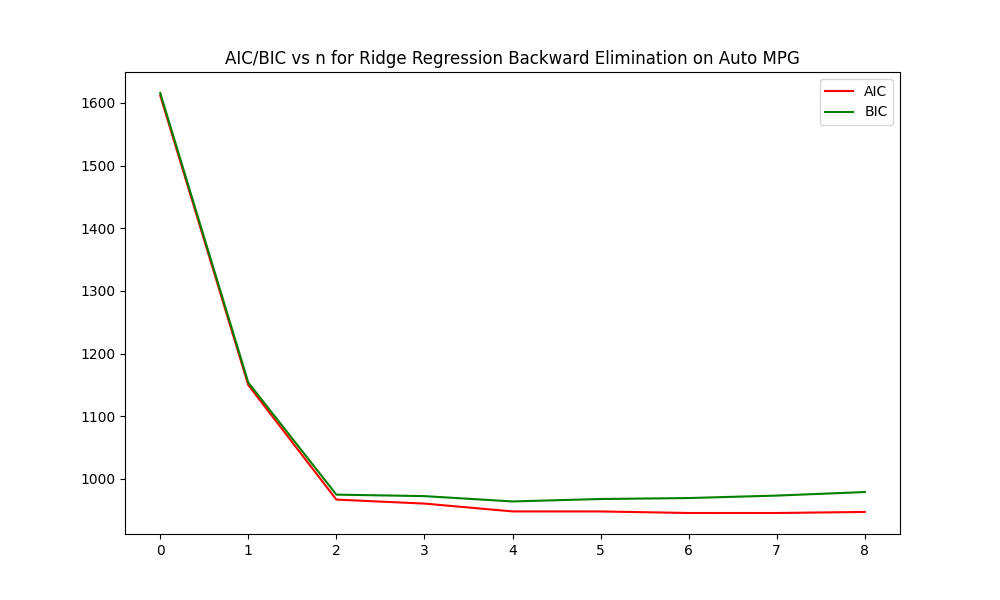
\includegraphics[width=\textwidth]{../Auto_MPG_Statsmodels_Plots/Statsmodels_Ridge_AIC_BIC_Backward.png}
     \end{subfigure}
     
     \caption{Auto MPG Ridge Regression Reversed Backward Elimination Quality of Fit Metrics\\ Top Left: Scalation $R^2$, Top Right: Scalation AIC/BIC\\ Bottom Left: Statsmodels $R^2$, Bottom Right: Statsmodels AIC/BIC}
     \label{fig:Auto MPG Ridge Regression Reversed Backward Elimination Quality of Fit Metrics}
\end{figure}

Scalation Stepwise Selection: displacement, weight, origin 2, modelyear, cylinders, acceleration, horsepower

Statsmodels Stepwise Selection: Null, weight, model year, origin 3, origin 2, displacement, horsepower, cylinders

\begin{figure}[H]
     \centering
     \captionsetup{justification=centering}
     % First Row
     \begin{subfigure}[b]{0.4\textwidth}
         \centering
         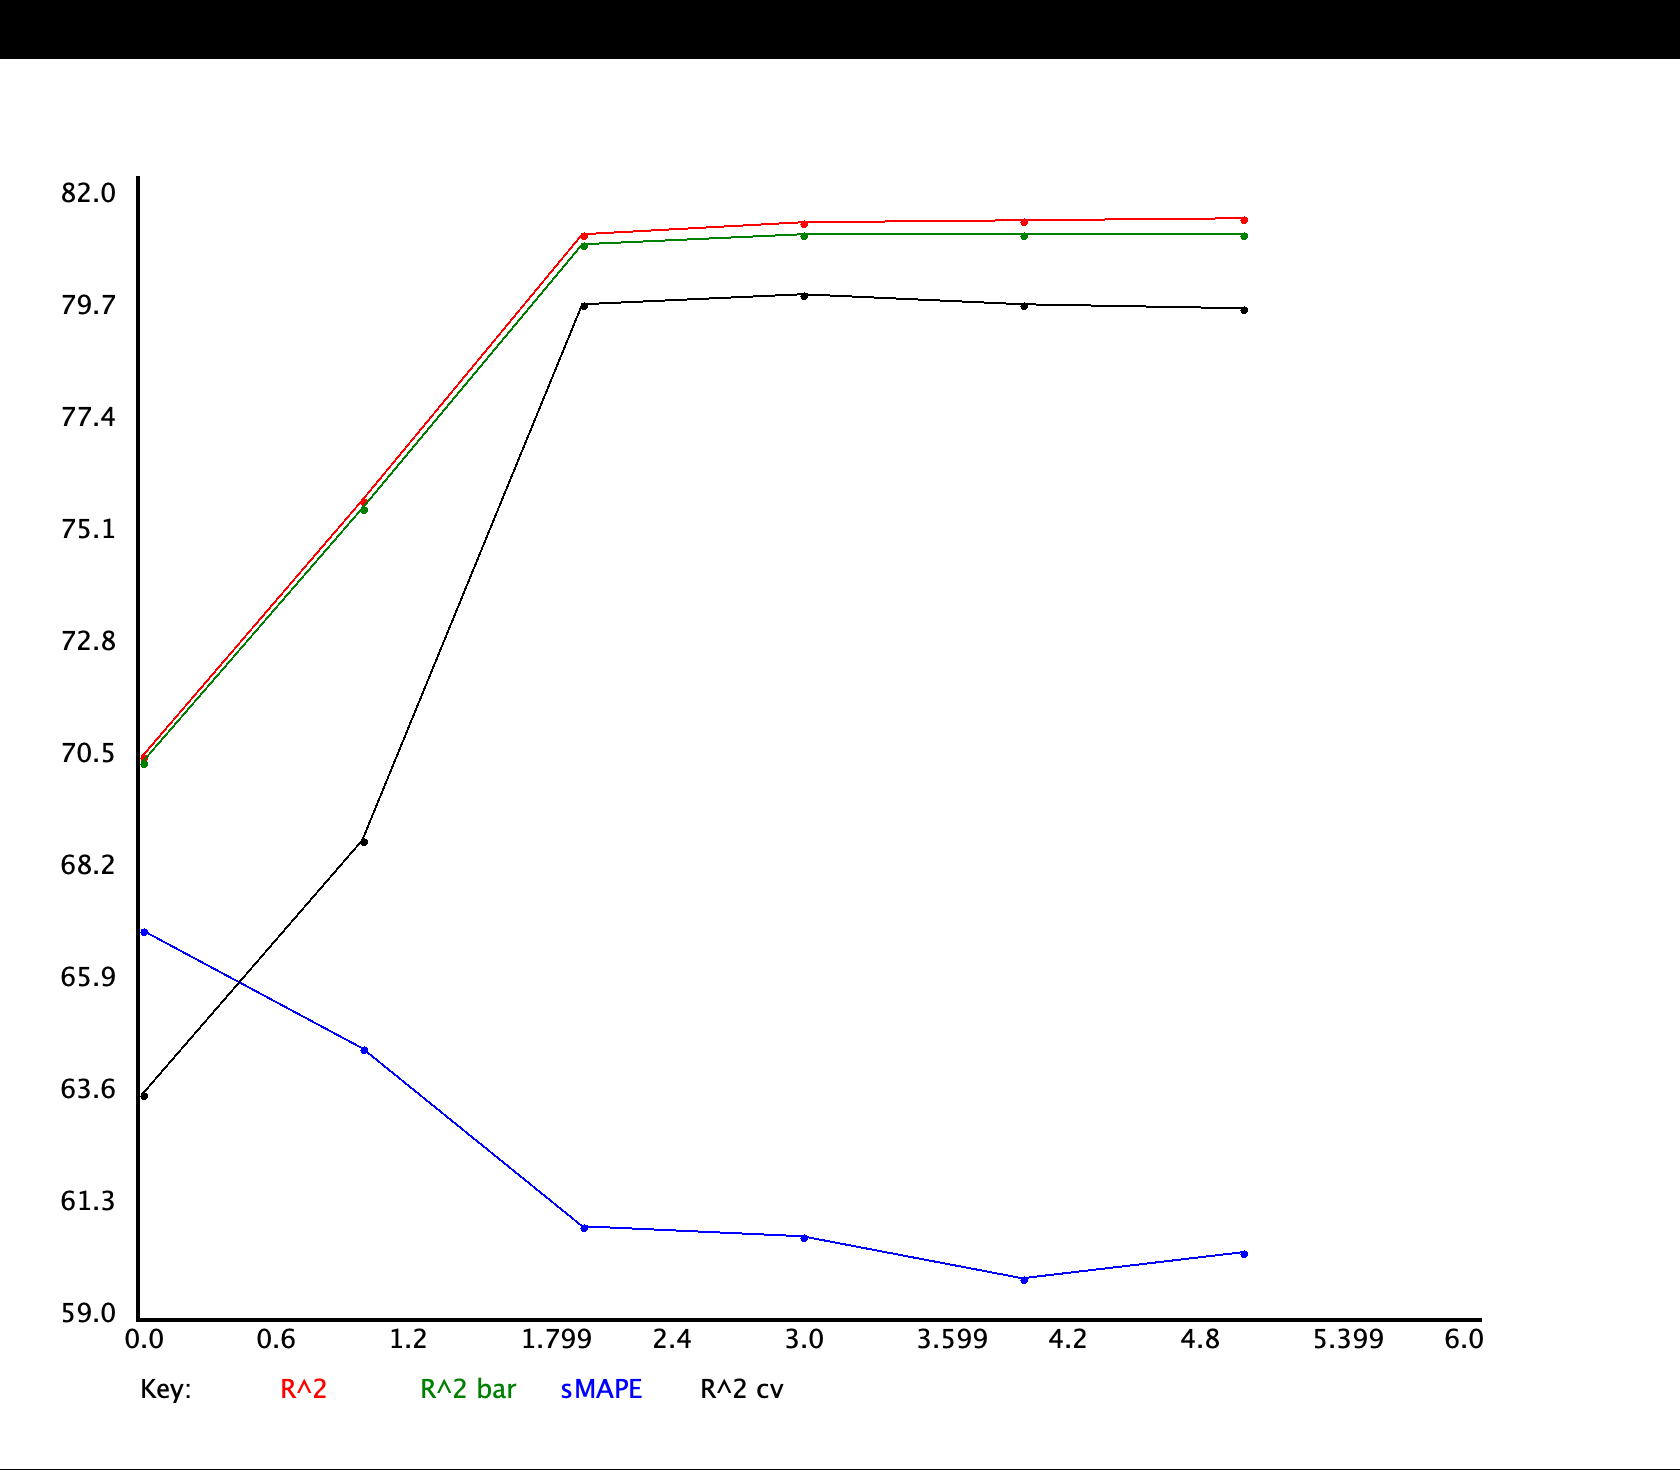
\includegraphics[width=\textwidth]{../Auto_MPG_Scalation_Plots/Scalation_Ridge_rSq_Stepwise.png}
     \end{subfigure}
     \hfill
     \begin{subfigure}[b]{0.4\textwidth}
         \centering
         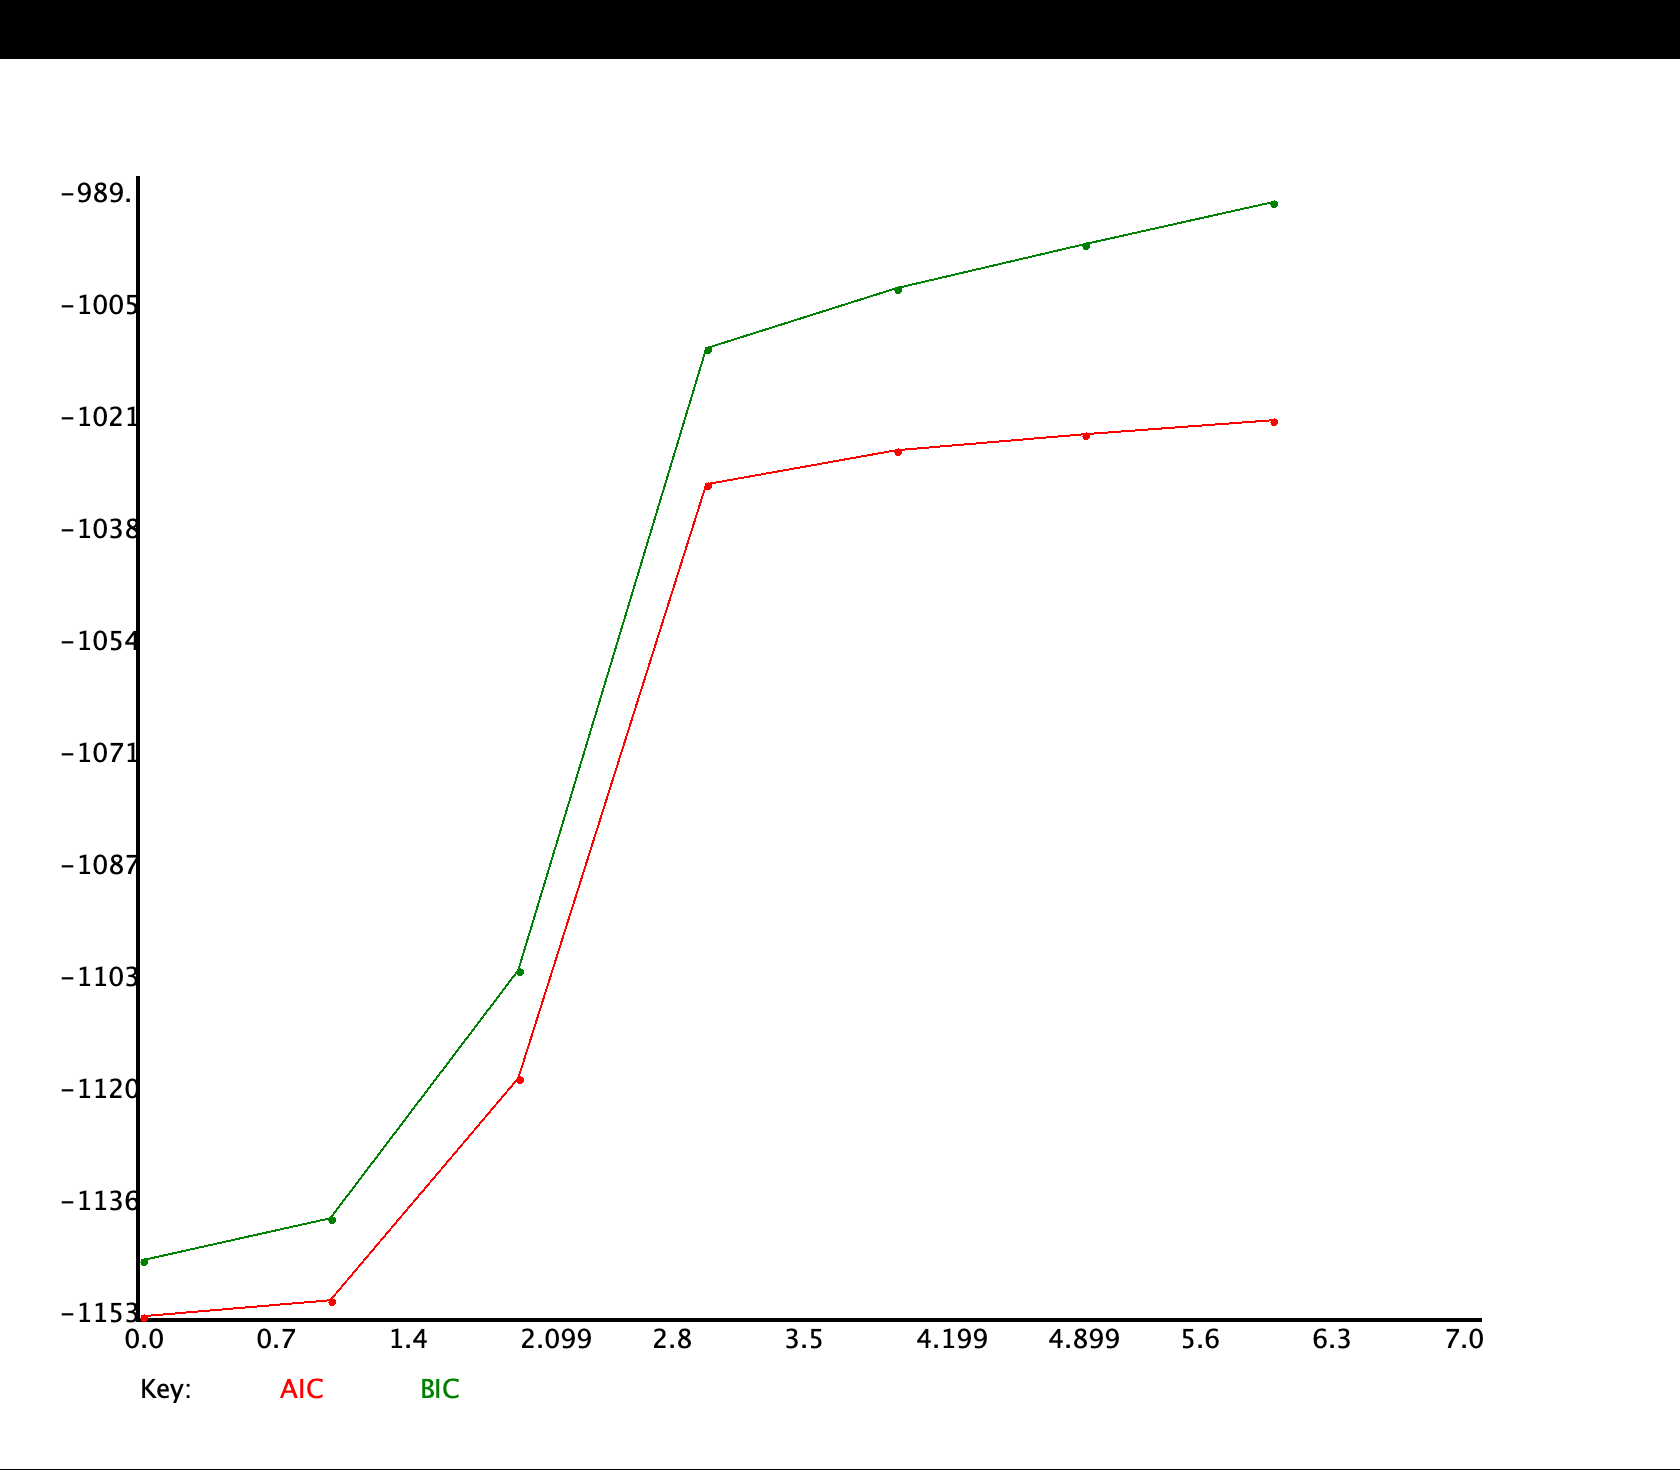
\includegraphics[width=\textwidth]{../Auto_MPG_Scalation_Plots/Scalation_Ridge_AIC_BIC_Stepwise.png}
     \end{subfigure}

     \vspace{10pt} % Add some vertical spacing between rows

     % Second Row
     \begin{subfigure}[b]{0.49\textwidth}
         \centering
         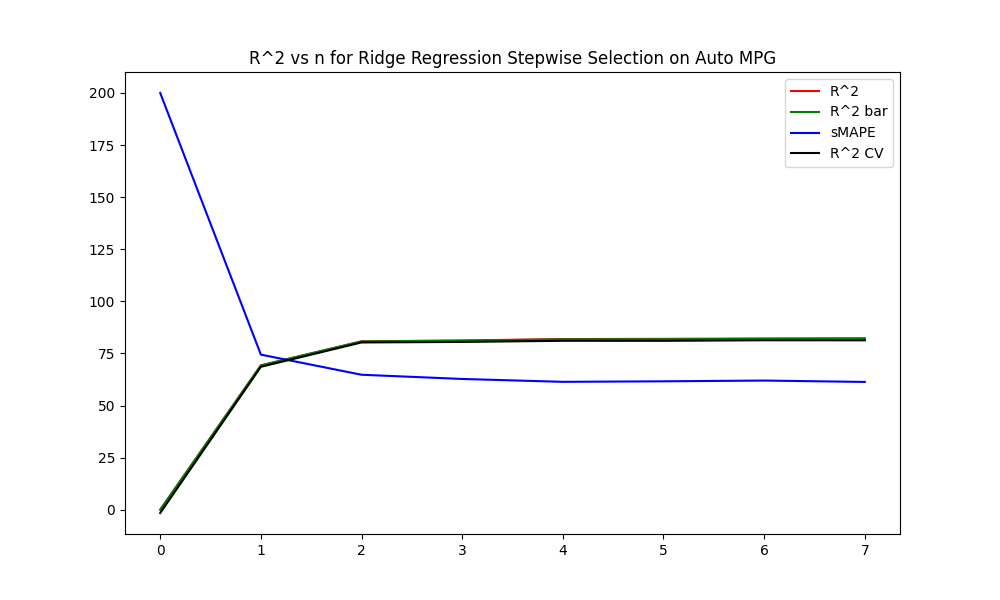
\includegraphics[width=\textwidth]{../Auto_MPG_Statsmodels_Plots/Statsmodels_Ridge_rSq_Stepwise.png}
     \end{subfigure}
     \hfill
     \begin{subfigure}[b]{0.49\textwidth}
         \centering
         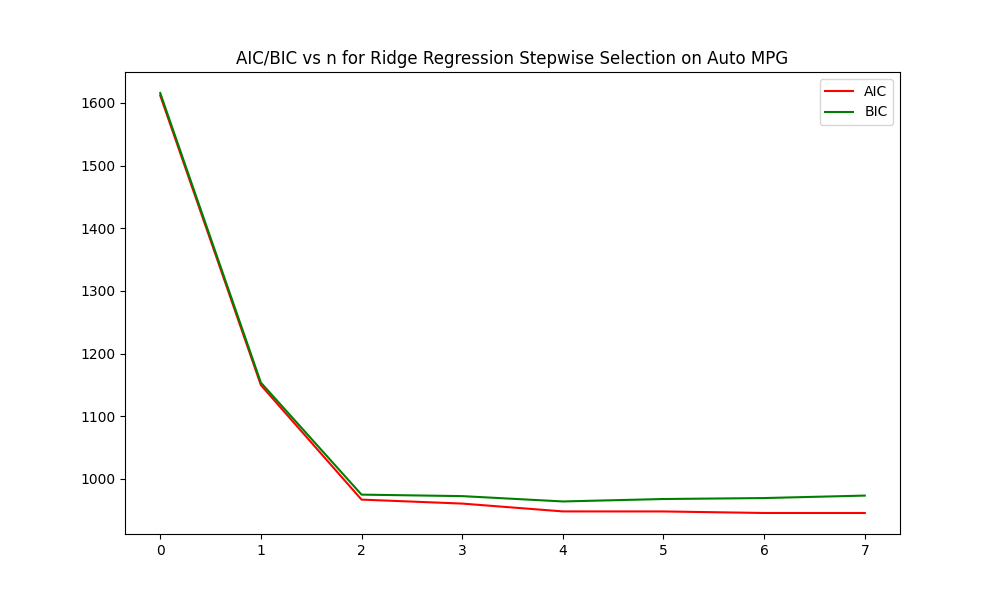
\includegraphics[width=\textwidth]{../Auto_MPG_Statsmodels_Plots/Statsmodels_Ridge_AIC_BIC_Stepwise.png}
     \end{subfigure}
     
     \caption{Auto MPG Ridge Regression Stepwise Selection Quality of Fit Metrics\\ Top Left: Scalation $R^2$, Top Right: Scalation AIC/BIC\\ Bottom Left: Statsmodels $R^2$, Bottom Right: Statsmodels AIC/BIC}
     \label{fig:Auto MPG Ridge Regression Stepwise Selection Quality of Fit Metrics}
\end{figure}

\subsection{Lasso Regression}

\subsubsection{Quality of Fit}

Scalation Auto MPG Lasso Lambda Used: $0.95$

\noindent Scalation Lasso Selected Features: displacement, cylinders, horsepower, weight, modelyear

\noindent Statsmodels Auto MPG Lasso alpha Used: $0.003$

\noindent Statsmodels Auto MPG Lasso Selected Features: displacement, cylinders, horsepower, weight, acceleration, model year, origin 2, origin 3

\begin{figure}[H]
     \centering
     \captionsetup{justification=centering}
     % First Row
     \begin{subfigure}[b]{0.4\textwidth}
         \centering
         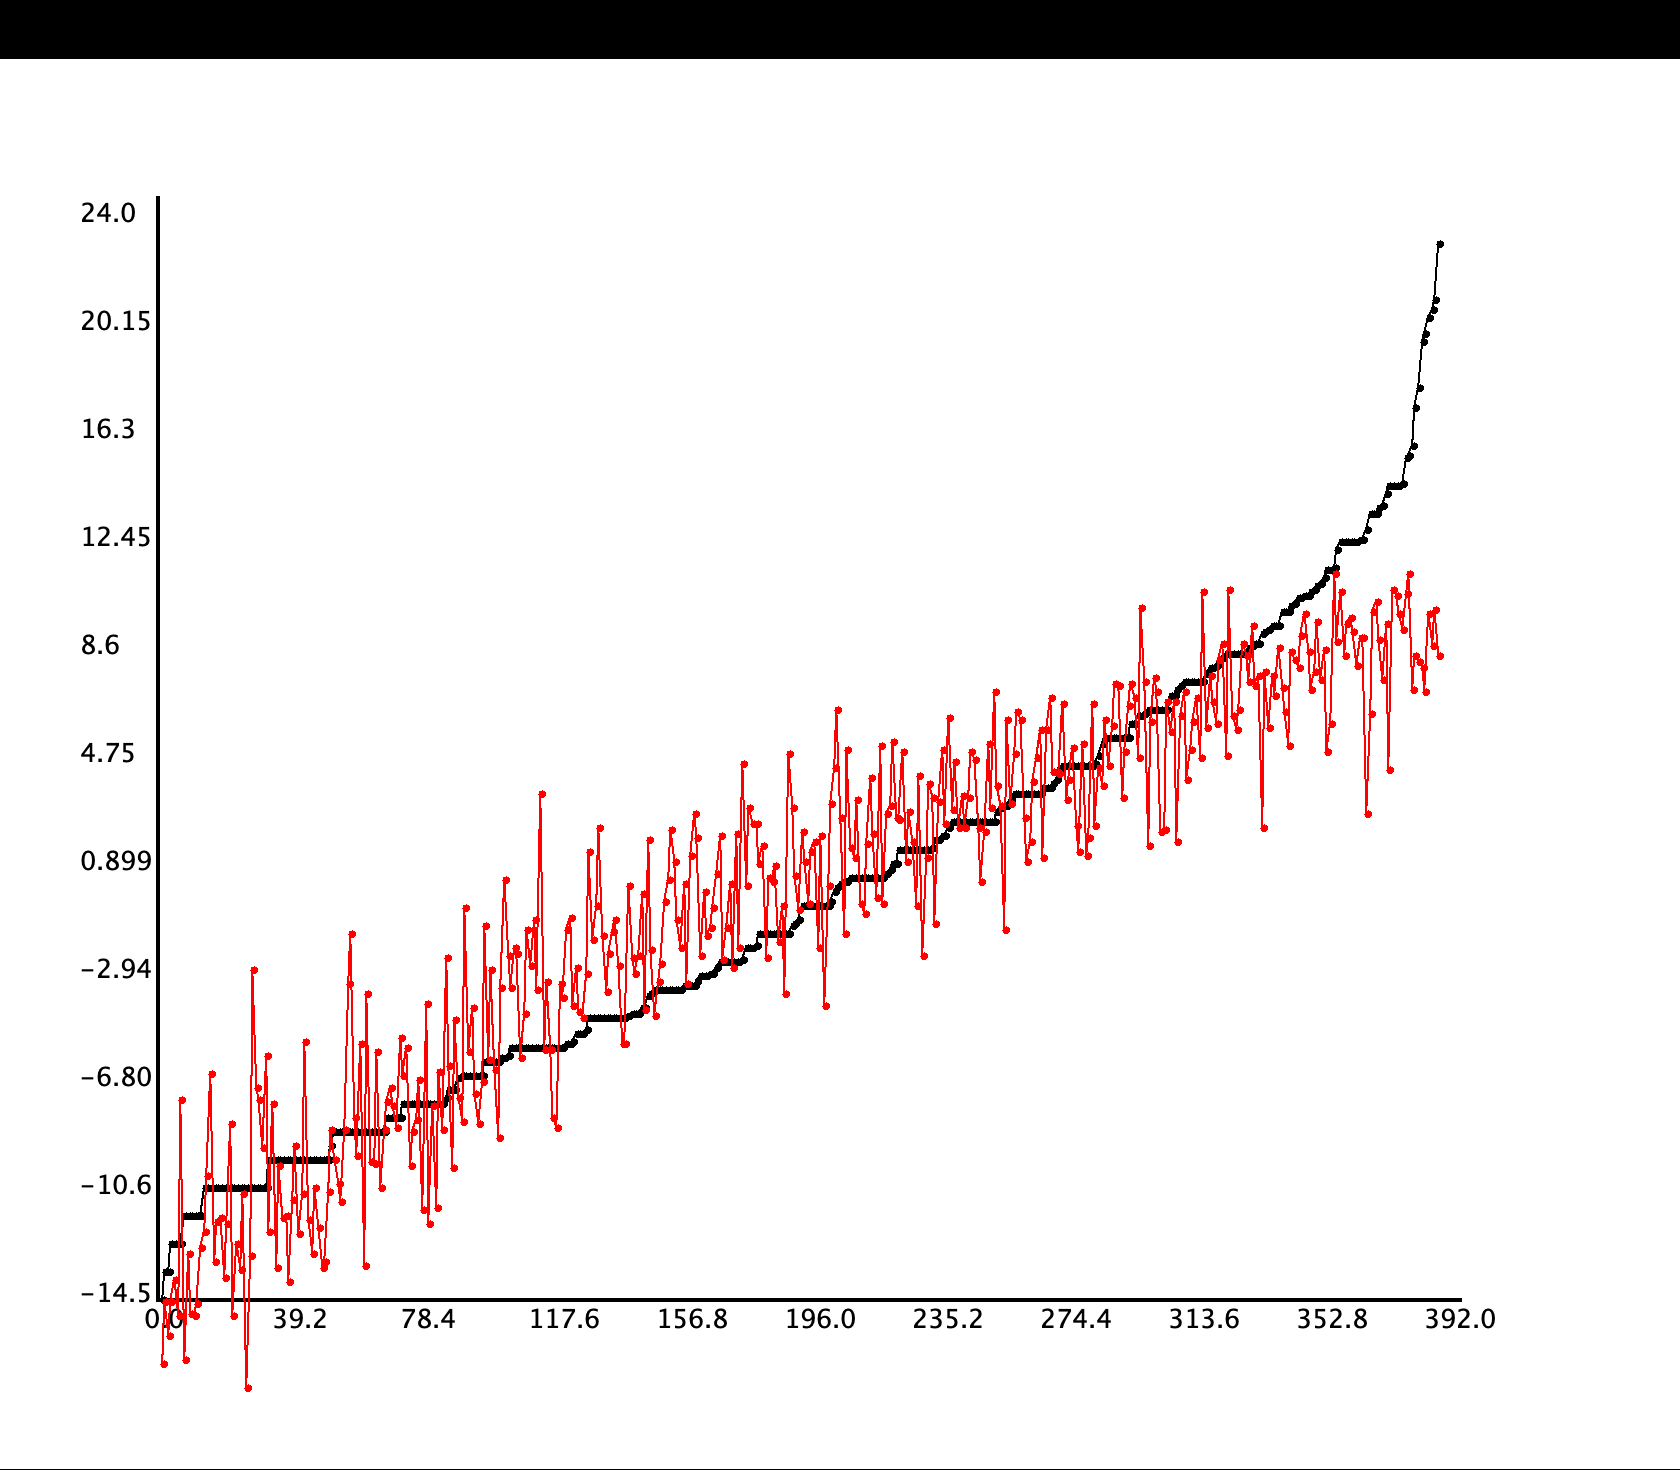
\includegraphics[width=\textwidth]{../Auto_MPG_Scalation_Plots/Scalation_Lasso_In_Sample.png}
     \end{subfigure}
     \hfill
     \begin{subfigure}[b]{0.4\textwidth}
         \centering
         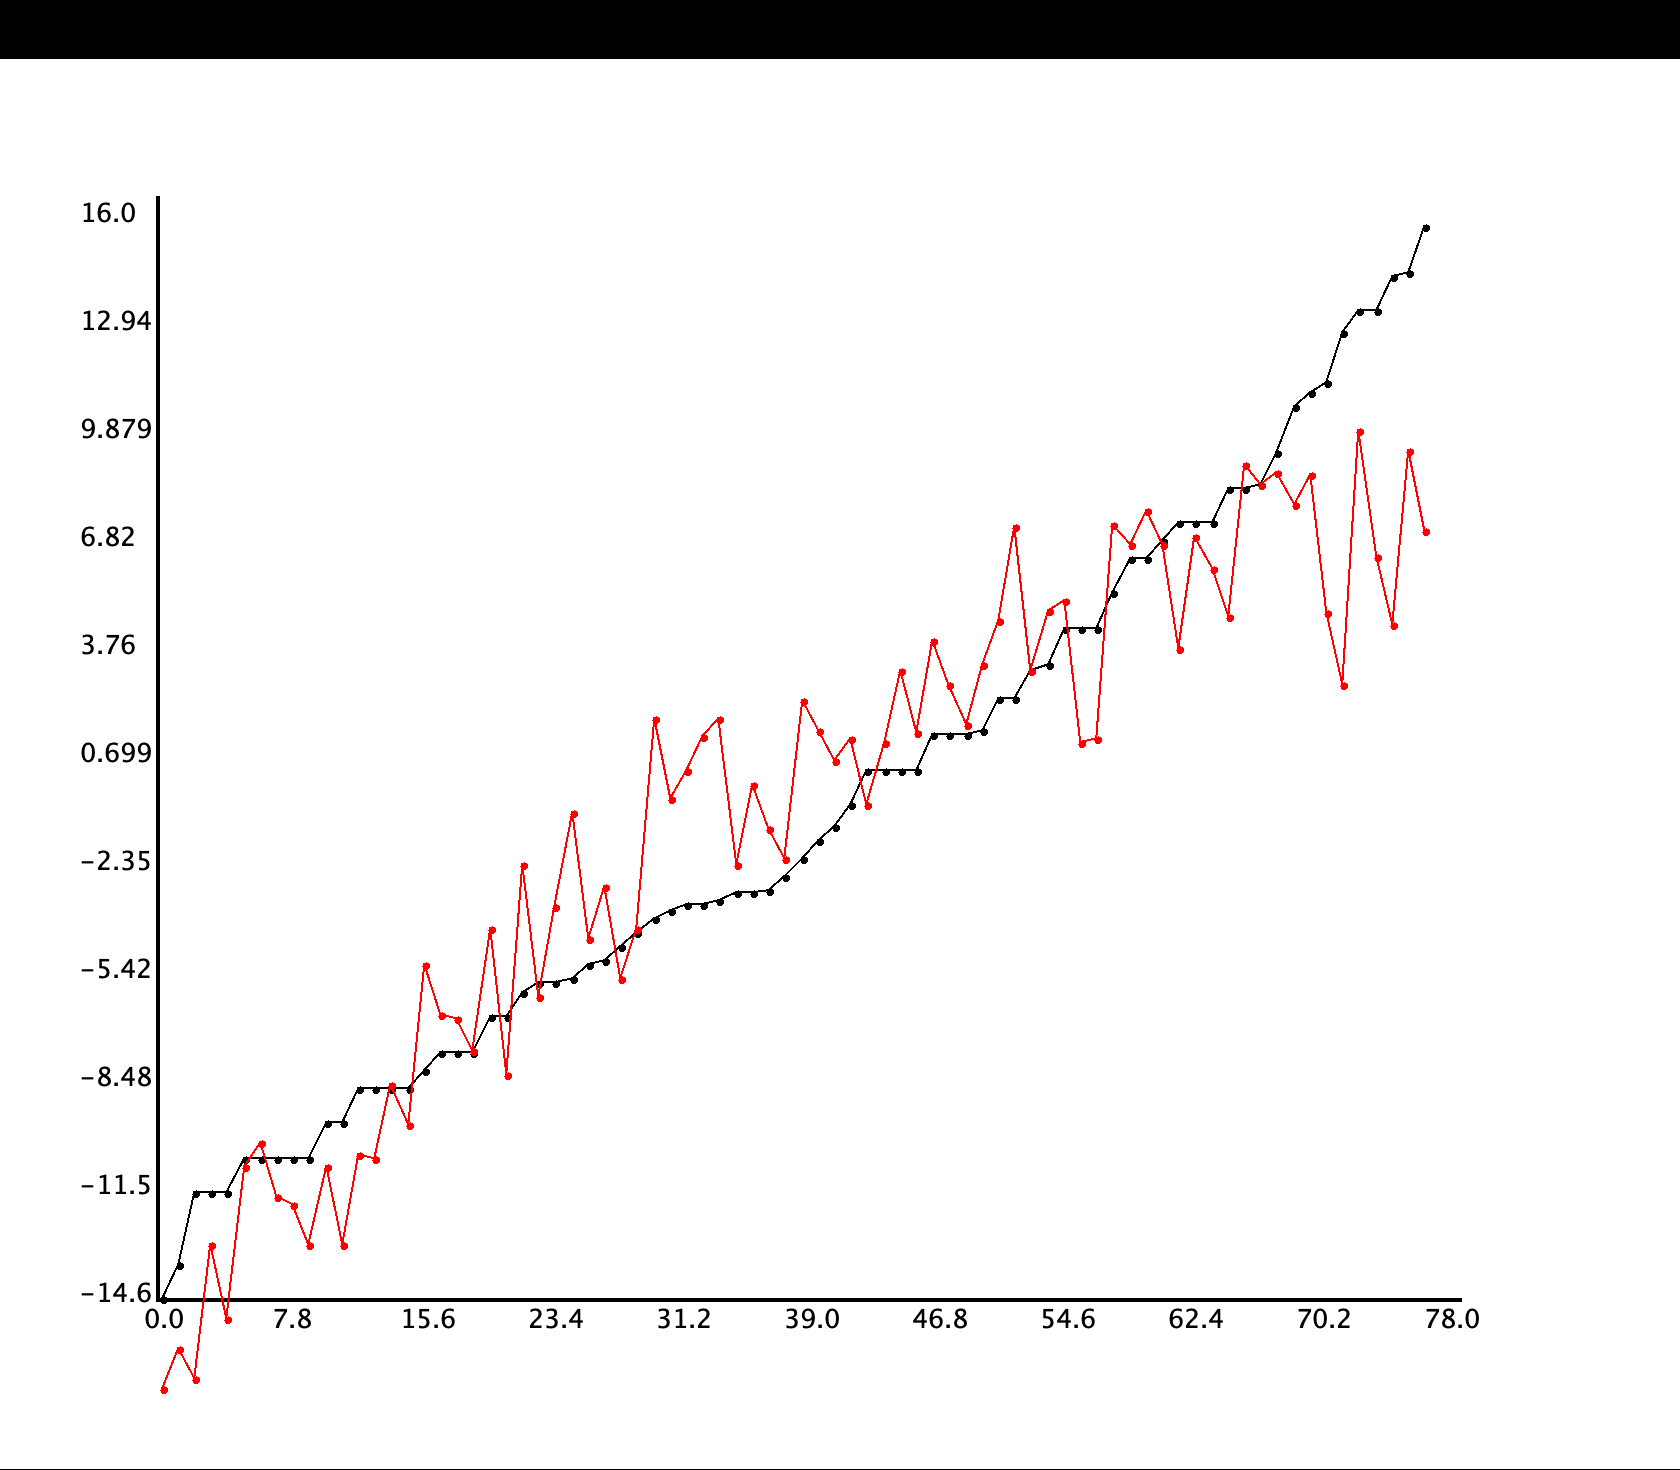
\includegraphics[width=\textwidth]{../Auto_MPG_Scalation_Plots/Scalation_Lasso_80_20.png}
     \end{subfigure}

     \vspace{10pt} % Add some vertical spacing between rows

     % Second Row
     \begin{subfigure}[b]{0.49\textwidth}
         \centering
         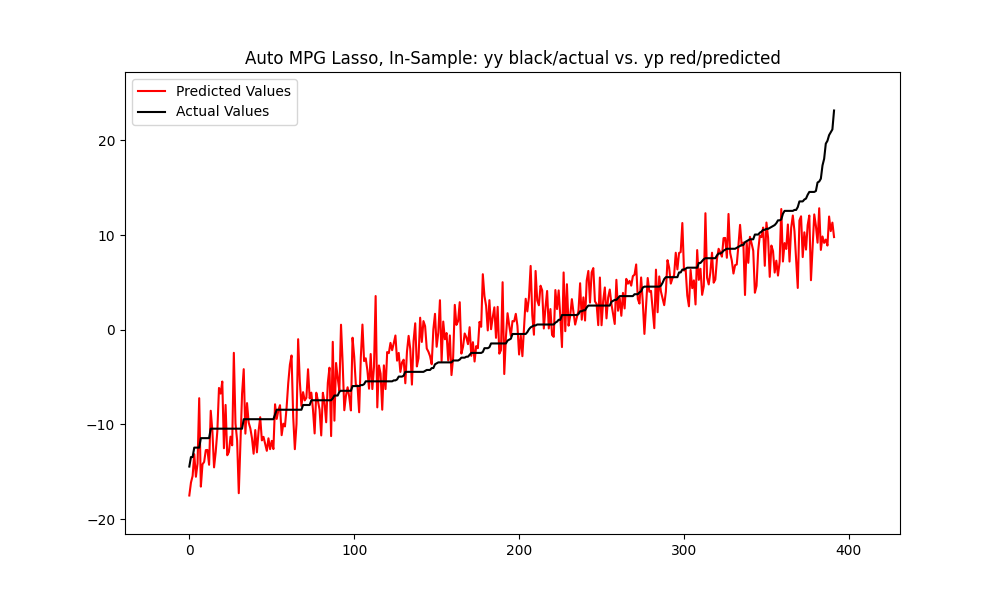
\includegraphics[width=\textwidth]{../Auto_MPG_Statsmodels_Plots/Statsmodels_Lasso_In_Sample.png}
     \end{subfigure}
     \hfill
     \begin{subfigure}[b]{0.49\textwidth}
         \centering
         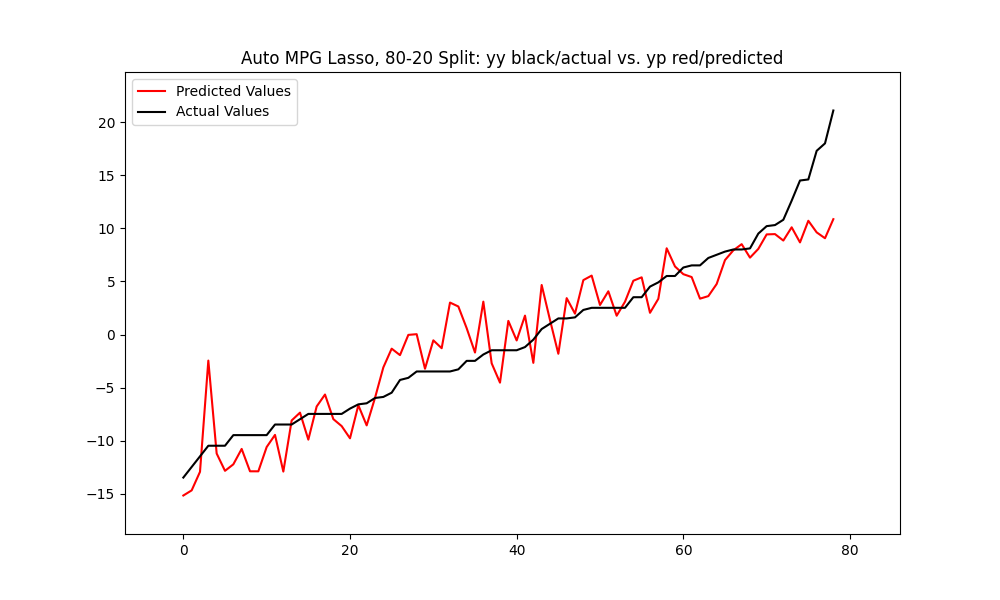
\includegraphics[width=\textwidth]{../Auto_MPG_Statsmodels_Plots/Statsmodels_Lasso_80_20.png}
     \end{subfigure}
     
     \caption{Auto MPG Lasso Regression Plots\\ Top Left: Scalation In-Sample, Top Right: Scalation Out-of-Sample\\ Bottom Left: Statsmodels In-Sample, Bottom Right: Statsmodels Out-of-Sample\\ black: actual y-values, red: predicted y-values}
     \label{fig:Auto MPG Lasso Regression Plots}
\end{figure}

\begin{table}[H]
\centering
\caption{Scalation - Auto MPG Lasso Regression}
\label{tab:Scalation - Auto MPG Lasso Regression}
\begin{tabular}{|c|c|c|} \hline 
Metric & In-Sample & 80-20 Split \\ \hline \hline 
rSq &0.808236 & 0.824643 \\ \hline 
rSqBar &0.804741 &      0.821446 \\ \hline 
sst &23819.0 &  4731.23 \\ \hline 
sse &4567.62 &  829.656 \\ \hline 
sde &3.41612 &  3.27330 \\ \hline 
mse0 &11.6521 & 10.6366 \\ \hline 
rmse &3.41352 & 3.26138 \\ \hline 
mae &2.61088 &  2.45626 \\ \hline 
smape &63.9389 &        63.3100 \\ \hline 
m &392.000 &    78.0000 \\ \hline 
dfr &7.00000 &  7.00000 \\ \hline 
df &384.000 &   384.000 \\ \hline 
fStat &231.209 &        257.974 \\ \hline 
aic &-1021.50 & -186.886 \\ \hline 
bic &-989.729 & -168.032 \\ \hline 
\end{tabular}
\end{table}

\begin{table}[H]
\centering
\caption{Statsmodels - Auto MPG Lasso Regression}
\label{tab:Statsmodels - Auto MPG Lasso Regression}
\begin{tabular}{|c|c|c|}\hline
Metric & In-Sample & 80-20 Split \\ \hline \hline
rSq & 0.8242 & 0.8387 \\ \hline
rSqBar & 0.8210 & 0.8228 \\ \hline
sst & 23818.9935 & 4910.2699 \\ \hline
sse & 4187.6288 & 791.8769 \\ \hline
sde & 3.3023 & 3.3396 \\ \hline
mse0 & 10.6827 & 10.0238 \\ \hline
rmse & 3.2684 & 3.1660 \\ \hline
mae & 2.5051 & 2.4146 \\ \hline
smape & 62.3436 & 58.3927 \\ \hline
m & 392.0000 & 79.0000 \\ \hline
dfr & 8.0000 & 8.0000 \\ \hline
df & 384.0000 & 71.0000 \\ \hline
fStat & 225.0213 & 46.1571 \\ \hline
aic & 944.5022 & 198.0917 \\ \hline
bic & 976.2723 & 217.0473 \\ \hline
\end{tabular}
\end{table}

\begin{table}[H]
\centering
\caption{Scalation - Auto MPG Lasso Regression CV}
\label{tab:Scalation - Auto MPG Lasso Regression CV}
\begin{tabular}{|c|c|c|c|c|c|}\hline
Metric & num folds & min & max & mean & stdev \\ \hline \hline
rSq & 5 & 0.786 & 0.825 & 0.801 & 0.015 \\ \hline
rSqBar & 5 & 0.782 & 0.821 & 0.797 & 0.016 \\ \hline
sst & 5 & 3962.818 & 5671.580 & 4700.481 & 620.767 \\ \hline
sse & 5 & 810.592 & 1181.163 & 936.371 & 155.141 \\ \hline
sde & 5 & 3.173 & 3.747 & 3.419 & 0.243 \\ \hline
mse0 & 5 & 10.392 & 15.143 & 12.005 & 1.989 \\ \hline
rmse & 5 & 3.224 & 3.891 & 3.456 & 0.280 \\ \hline
mae & 5 & 2.456 & 2.809 & 2.651 & 0.137 \\ \hline
smape & 5 & 60.657 & 70.362 & 65.555 & 4.384 \\ \hline
m & 5 & 78.000 & 78.000 & 78.000 & 0.000 \\ \hline
dfr & 5 & 7.000 & 7.000 & 7.000 & 0.000 \\ \hline
df & 5 & 384.000 & 384.000 & 384.000 & 0.000 \\ \hline
fStat & 5 & 201.634 & 257.949 & 222.193 & 22.469 \\ \hline
aic & 5 & -203.501 & -185.984 & -191.930 & 7.333 \\ \hline
bic & 5 & -184.647 & -167.131 & -173.076 & 7.333 \\ \hline
\end{tabular}
\end{table}

\begin{table}[H]
\centering
\caption{Statsmodels - Auto MPG Lasso Regression CV}
\label{tab:Statsmodels - Auto MPG Lasso Regression CV}
\begin{tabular}{|c|c|c|c|c|c|}\hline
Metric & num folds & min & max & mean & stdev \\ \hline \hline
rSq & 5 & 0.7319 & 0.8438 & 0.8103 & 0.0406 \\ \hline
rSqBar & 5 & 0.7051 & 0.8282 & 0.7915 & 0.0447 \\ \hline
sst & 5 & 3880.9704 & 5093.9237 & 4721.1782 & 441.3031 \\ \hline
sse & 5 & 789.6858 & 1040.5934 & 878.1148 & 92.0911 \\ \hline
sde & 5 & 3.3350 & 3.8556 & 3.5274 & 0.1885 \\ \hline
mse0 & 5 & 9.9960 & 13.3409 & 11.2044 & 1.2131 \\ \hline
rmse & 5 & 3.1616 & 3.6525 & 3.3426 & 0.1779 \\ \hline
mae & 5 & 2.3930 & 2.9873 & 2.5643 & 0.2193 \\ \hline
smape & 5 & 55.6016 & 73.3892 & 63.2520 & 6.5983 \\ \hline
m & 5 & 78.0000 & 79.0000 & 78.4000 & 0.4899 \\ \hline
dfr & 5 & 8.0000 & 8.0000 & 8.0000 & 0.0000 \\ \hline
df & 5 & 70.0000 & 71.0000 & 70.4000 & 0.4899 \\ \hline
fStat & 5 & 23.8838 & 47.2772 & 39.3824 & 8.3757 \\ \hline
aic & 5 & 197.1402 & 218.0853 & 204.9728 & 7.6207 \\ \hline
bic & 5 & 215.9939 & 236.9390 & 223.8672 & 7.6001 \\ \hline
\end{tabular}
\end{table}

\subsubsection{Feature Selection}

Scalation Forward Selection: displacement, weight, origin 2, modelyear, cylinders, acceleration, horsepower, origin 3

Statsmodels Forward Selection: Null, weight, model year, origin 3, origin 2, displacement, horsepower, cylinders, acceleration

\begin{figure}[H]
     \centering
     \captionsetup{justification=centering}
     % First Row
     \begin{subfigure}[b]{0.4\textwidth}
         \centering
         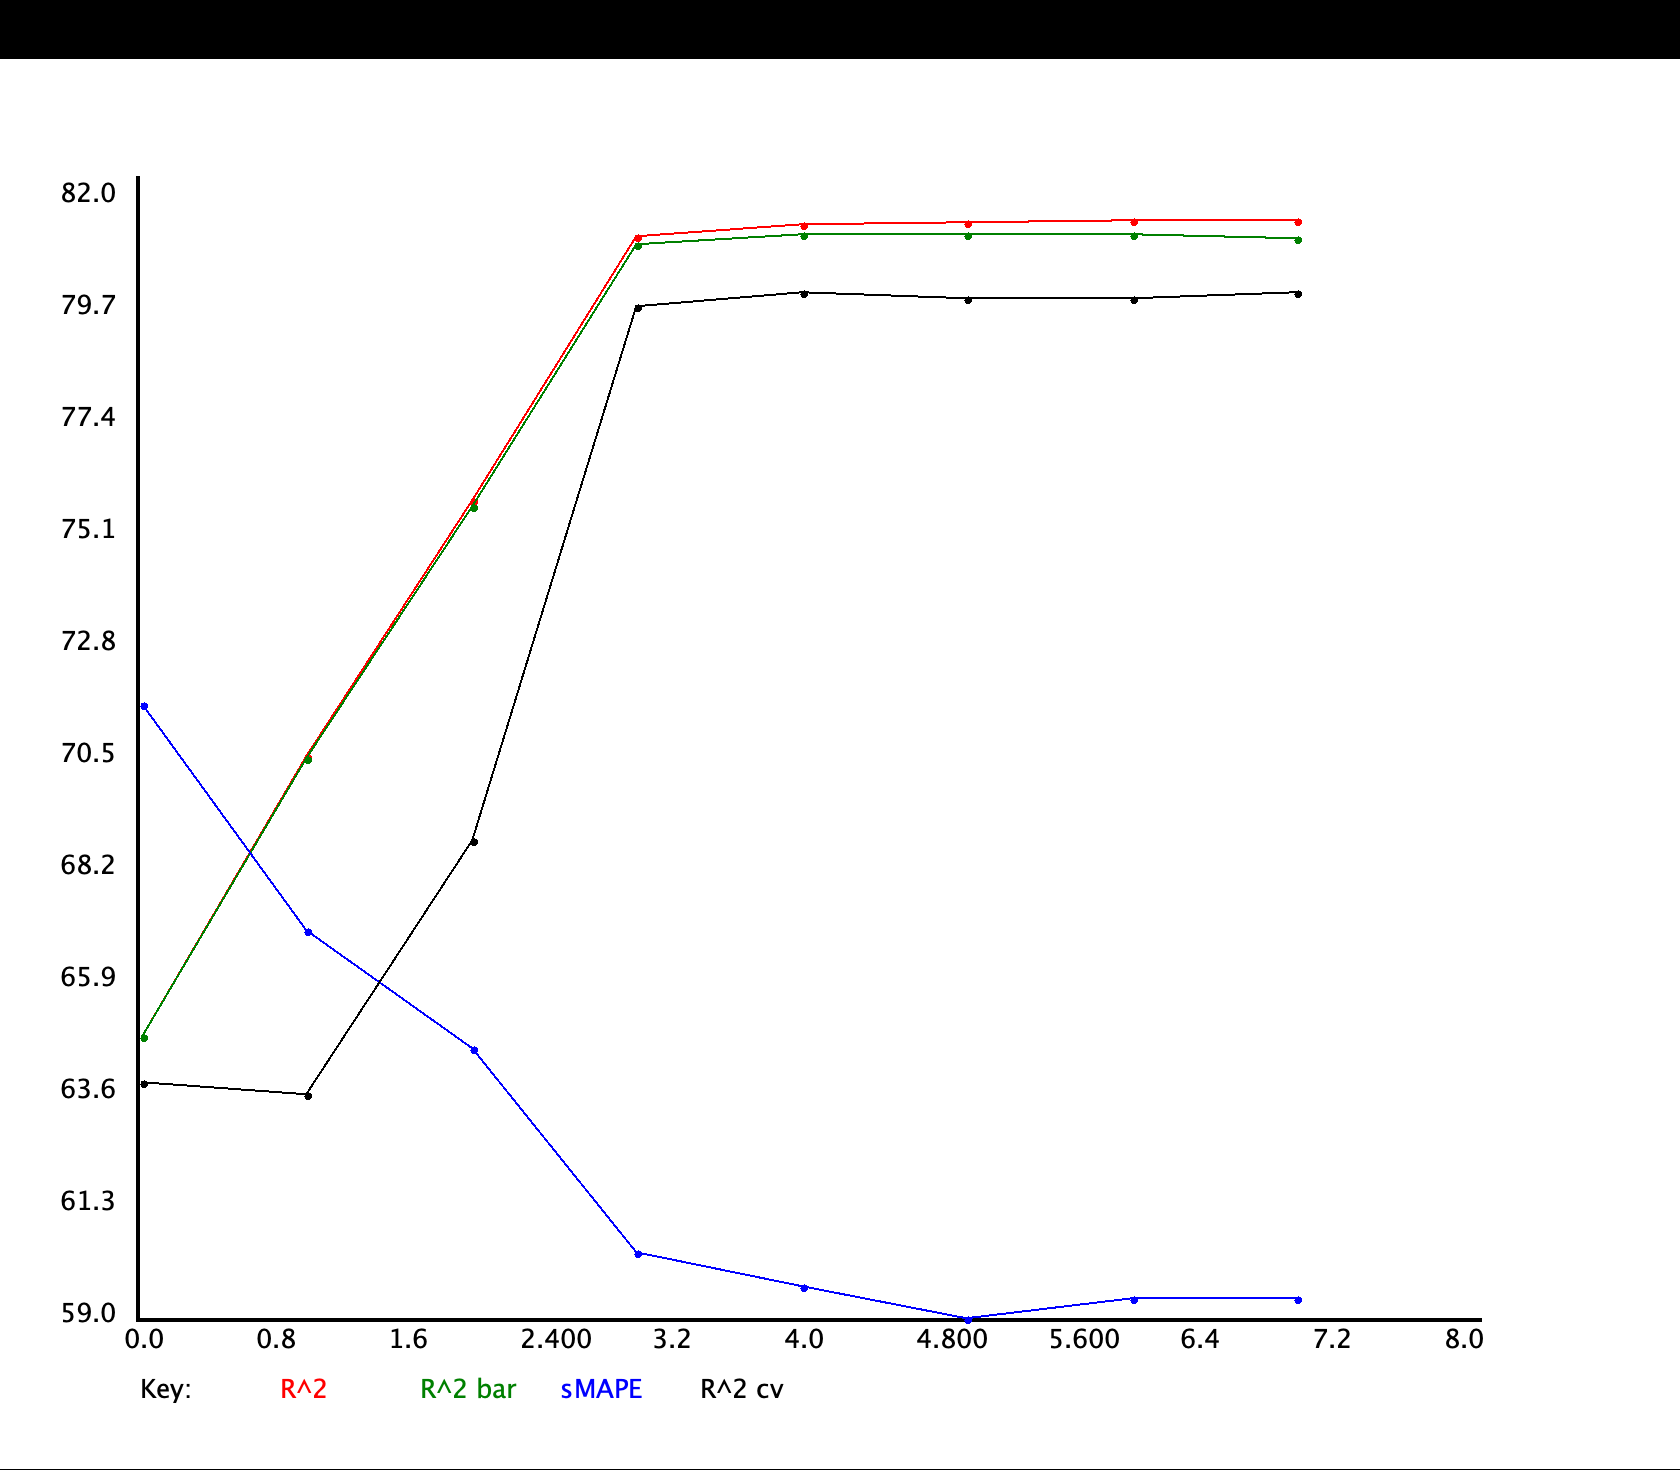
\includegraphics[width=\textwidth]{../Auto_MPG_Scalation_Plots/Scalation_Lasso_rSq_Forward.png}
     \end{subfigure}
     \hfill
     \begin{subfigure}[b]{0.4\textwidth}
         \centering
         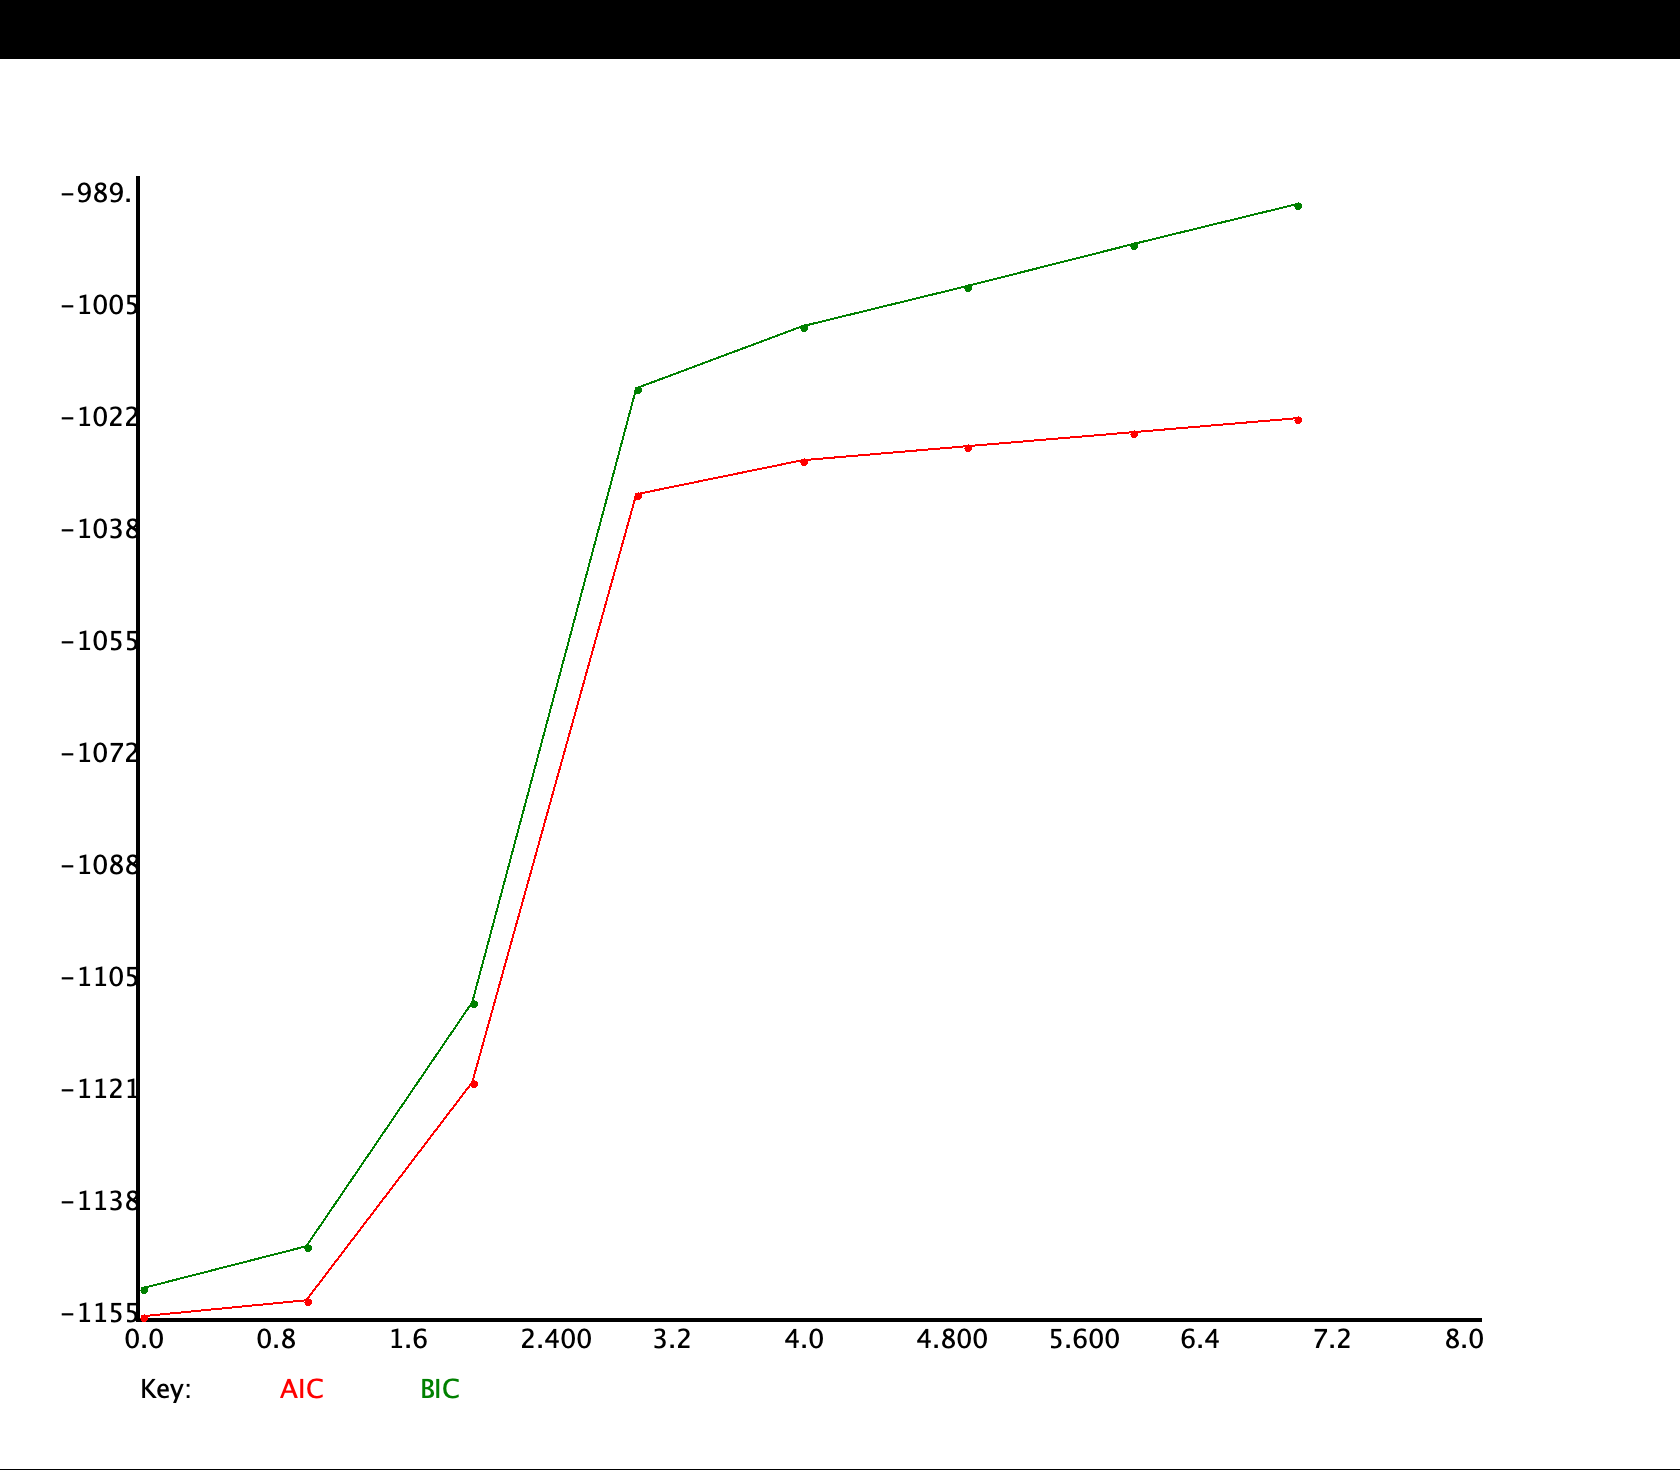
\includegraphics[width=\textwidth]{../Auto_MPG_Scalation_Plots/Scalation_Lasso_AIC_BIC_Forward.png}
     \end{subfigure}

     \vspace{10pt} % Add some vertical spacing between rows

     % Second Row
     \begin{subfigure}[b]{0.49\textwidth}
         \centering
         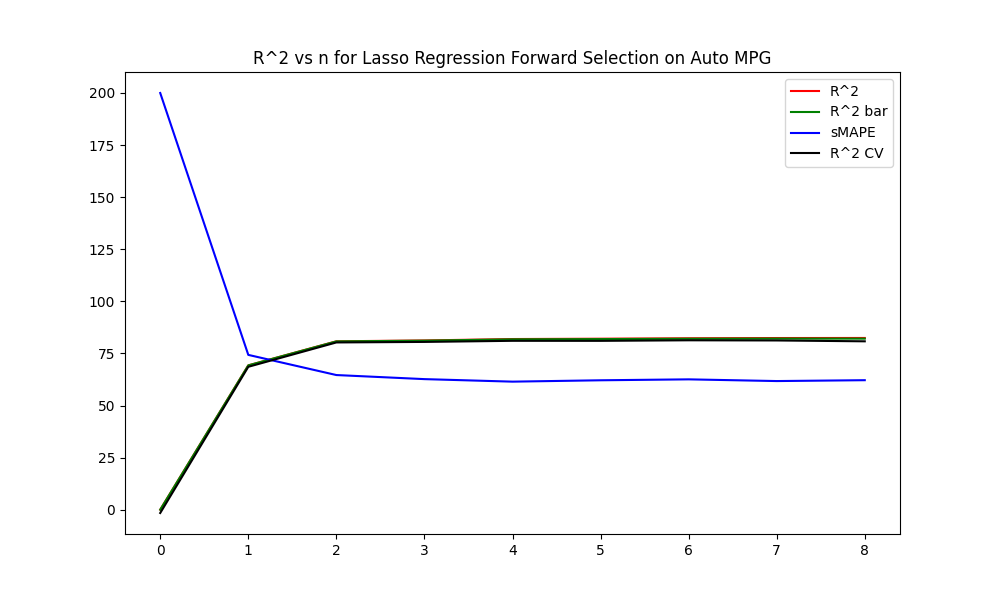
\includegraphics[width=\textwidth]{../Auto_MPG_Statsmodels_Plots/Statsmodels_Lasso_rSq_Forward.png}
     \end{subfigure}
     \hfill
     \begin{subfigure}[b]{0.49\textwidth}
         \centering
         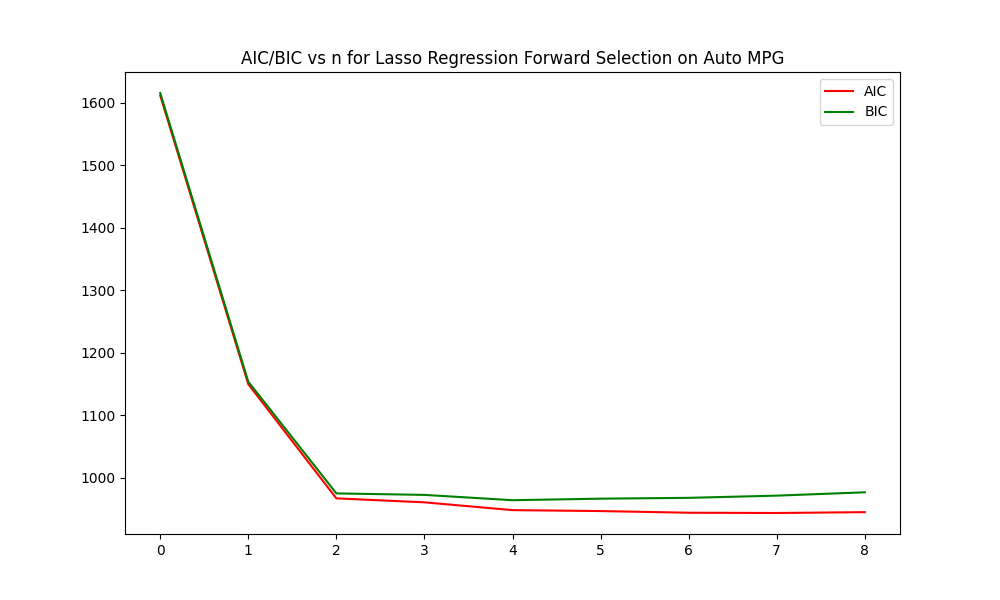
\includegraphics[width=\textwidth]{../Auto_MPG_Statsmodels_Plots/Statsmodels_Lasso_AIC_BIC_Forward.png}
     \end{subfigure}
     
     \caption{Auto MPG Lasso Regression Forward Selection Quality of Fit Metrics\\ Top Left: Scalation $R^2$, Top Right: Scalation AIC/BIC\\ Bottom Left: Statsmodels $R^2$, Bottom Right: Statsmodels AIC/BIC}
     \label{fig:Auto MPG Lasso Regression Forward Selection Quality of Fit Metrics}
\end{figure}

Scalation Backward Elimination Reversed: displacement, weight, cylinders, modelyear, acceleration, horsepower, origin 3, origin 2

Statsmodels Backward Elimination Reversed: Null, weight, model year, origin 3, origin 2, displacement, horsepower, cylinders, acceleration

\begin{figure}[H]
     \centering
     \captionsetup{justification=centering}
     % First Row
     \begin{subfigure}[b]{0.4\textwidth}
         \centering
         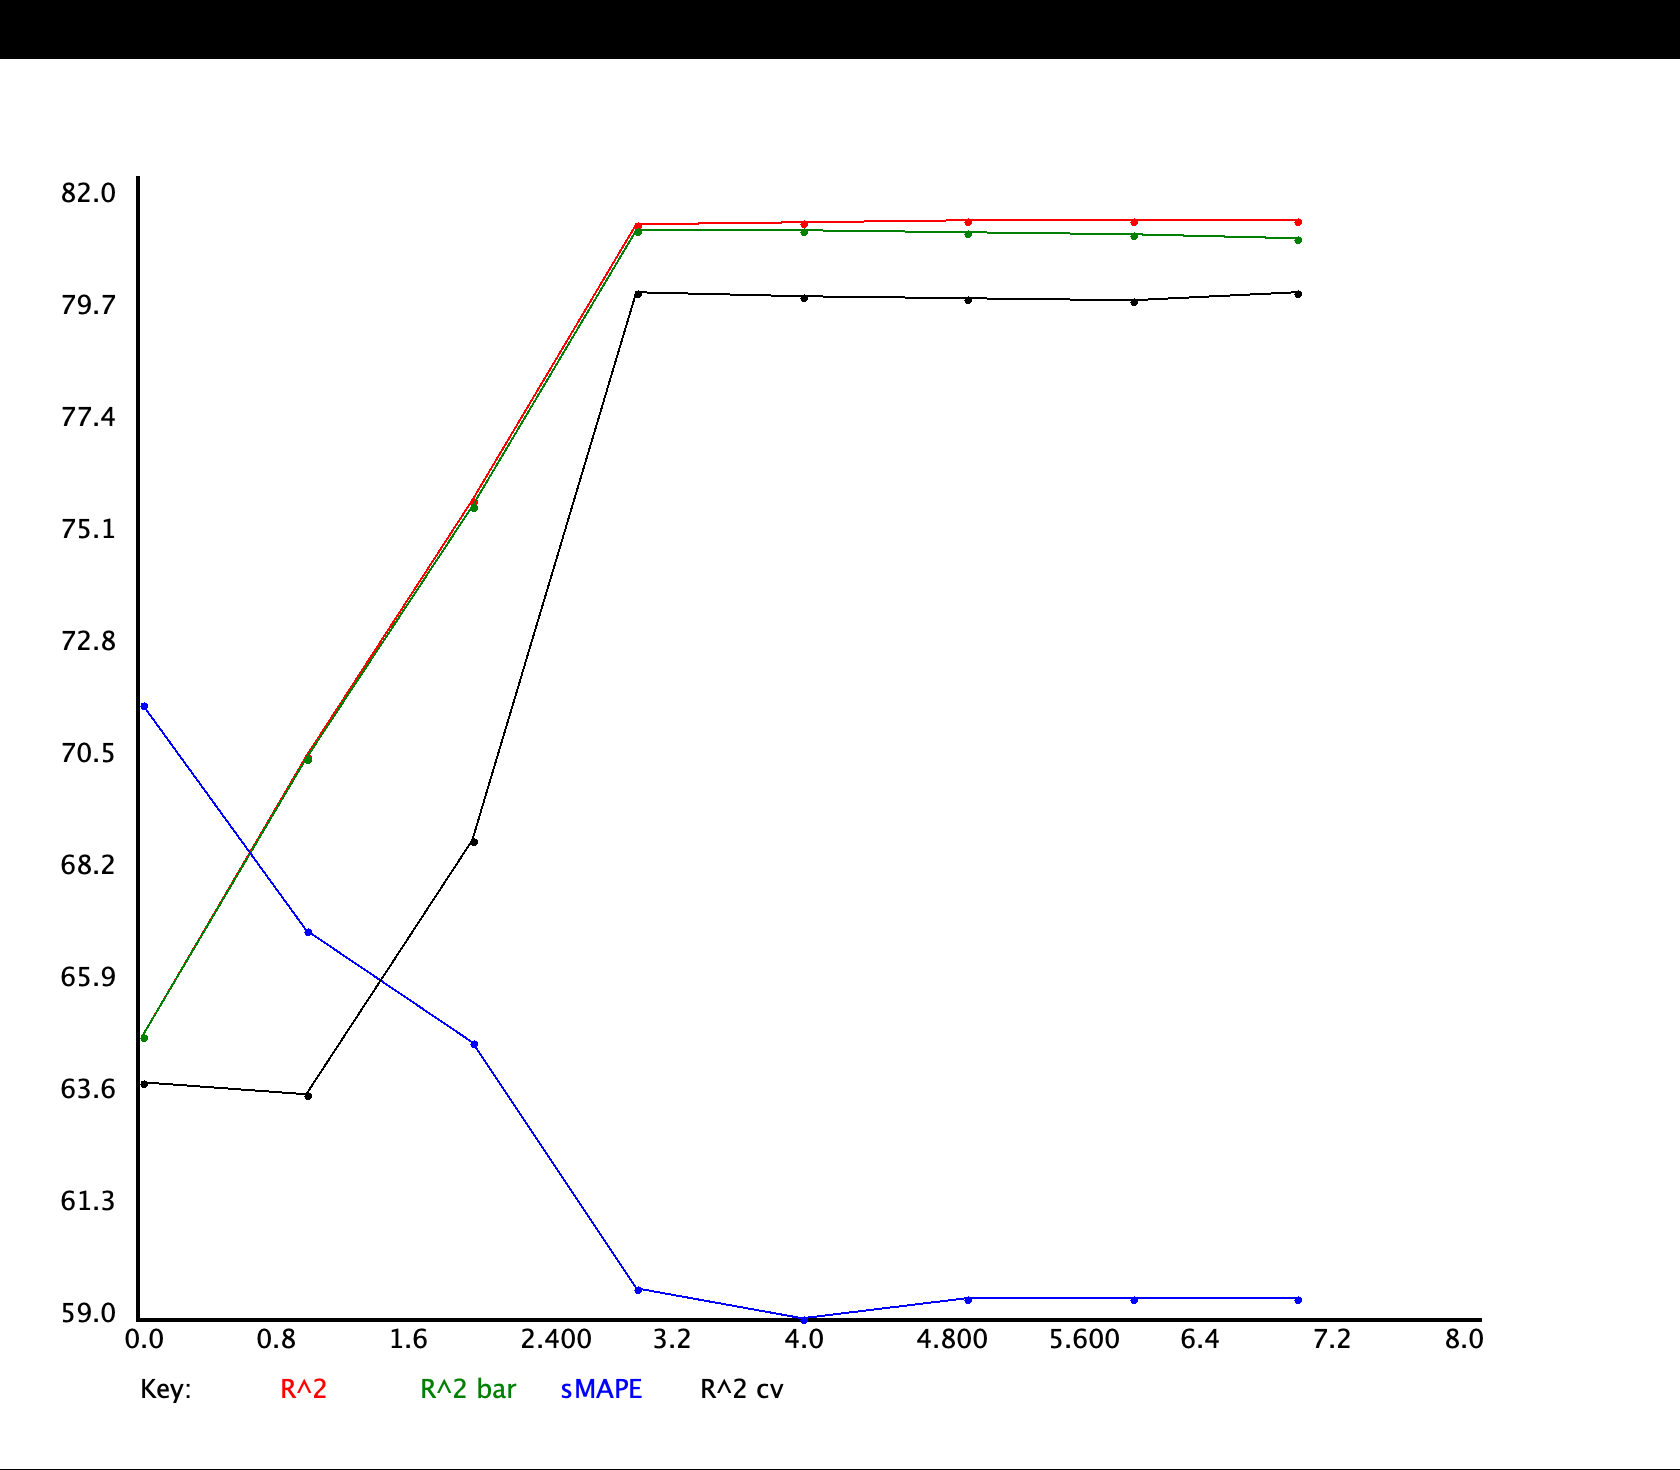
\includegraphics[width=\textwidth]{../Auto_MPG_Scalation_Plots/Scalation_Lasso_rSq_Backward.png}
     \end{subfigure}
     \hfill
     \begin{subfigure}[b]{0.4\textwidth}
         \centering
         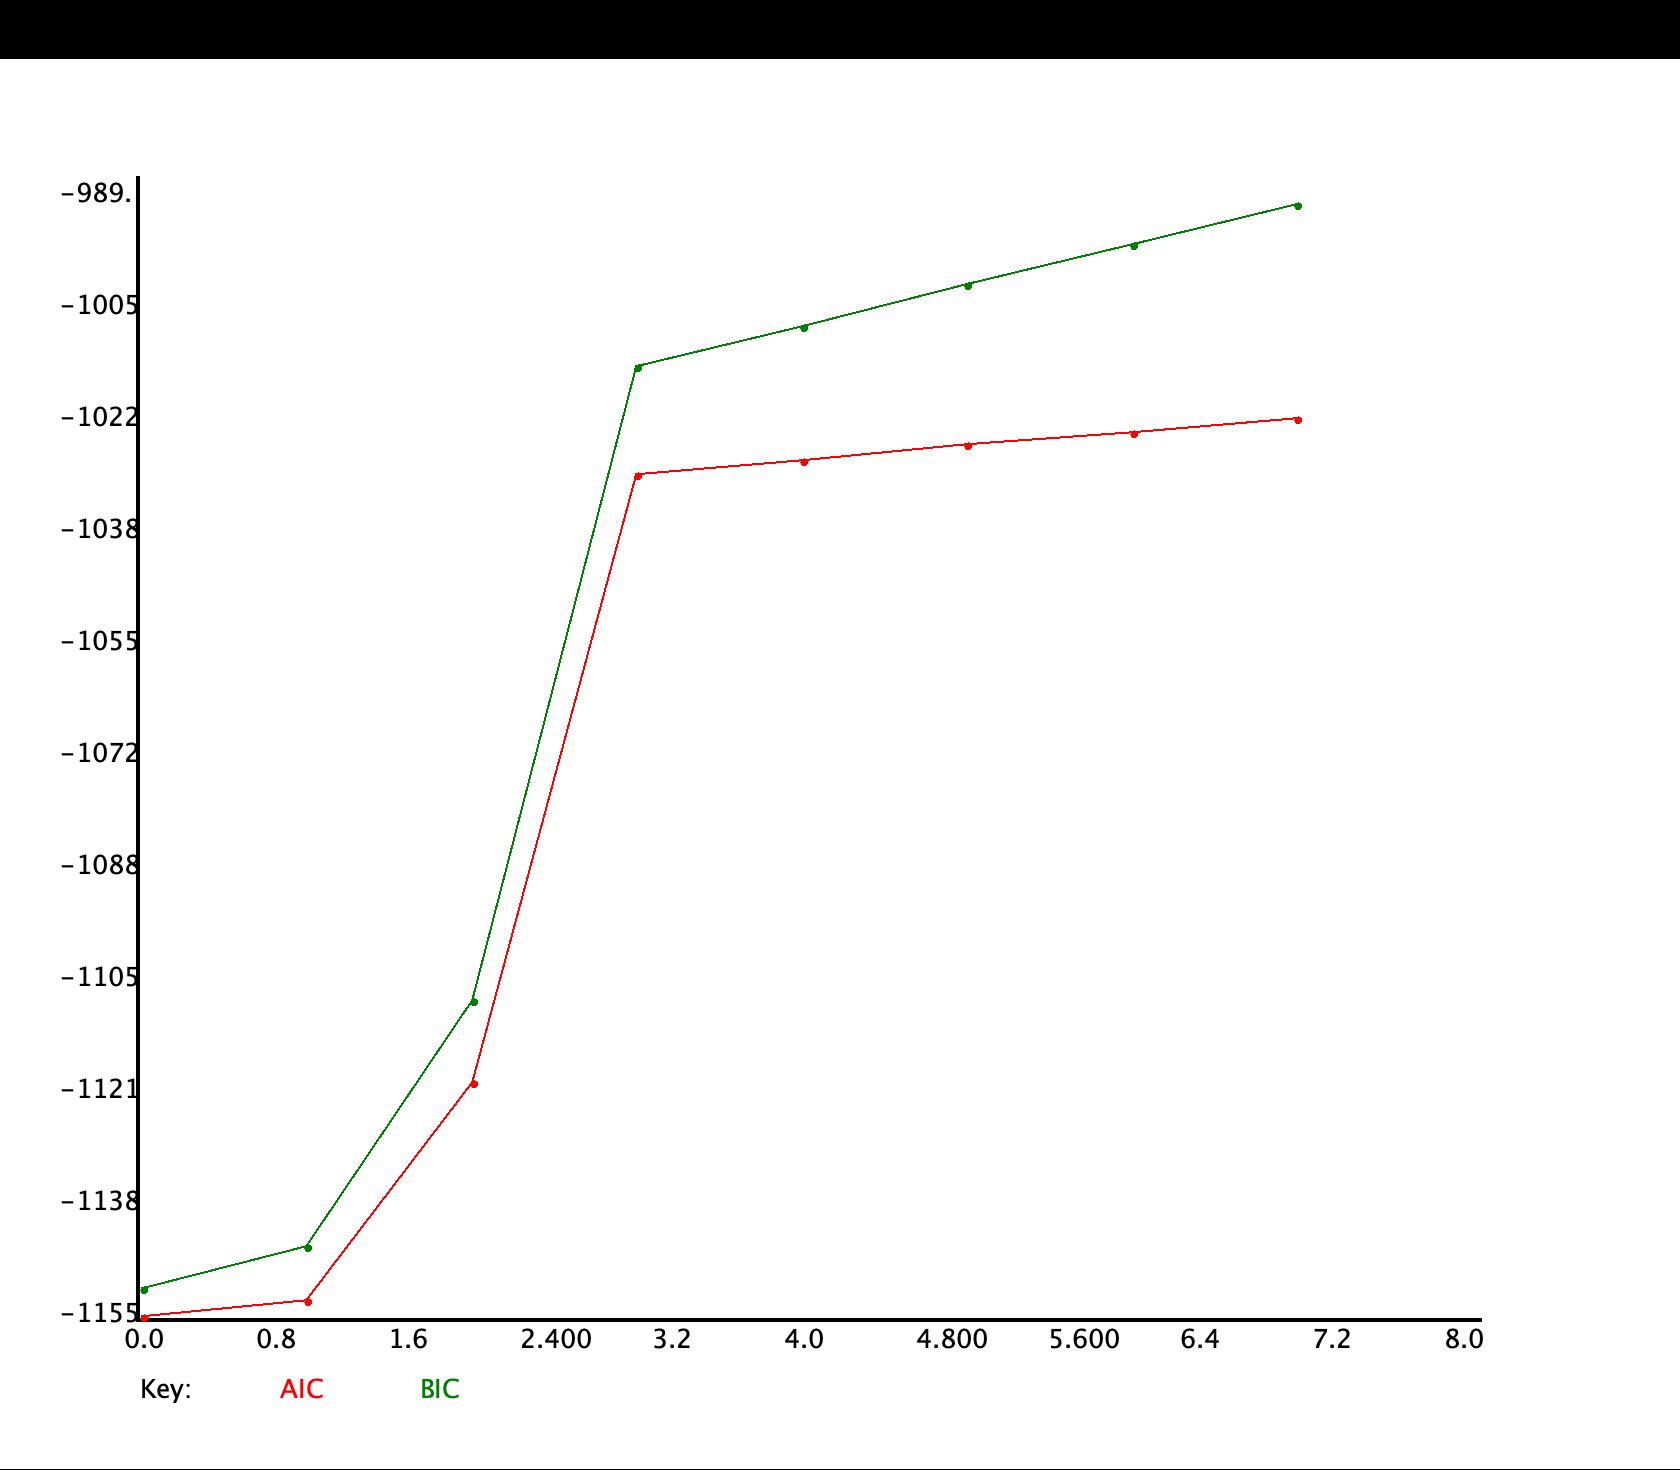
\includegraphics[width=\textwidth]{../Auto_MPG_Scalation_Plots/Scalation_Lasso_AIC_BIC_Backward.png}
     \end{subfigure}

     \vspace{10pt} % Add some vertical spacing between rows

     % Second Row
     \begin{subfigure}[b]{0.49\textwidth}
         \centering
         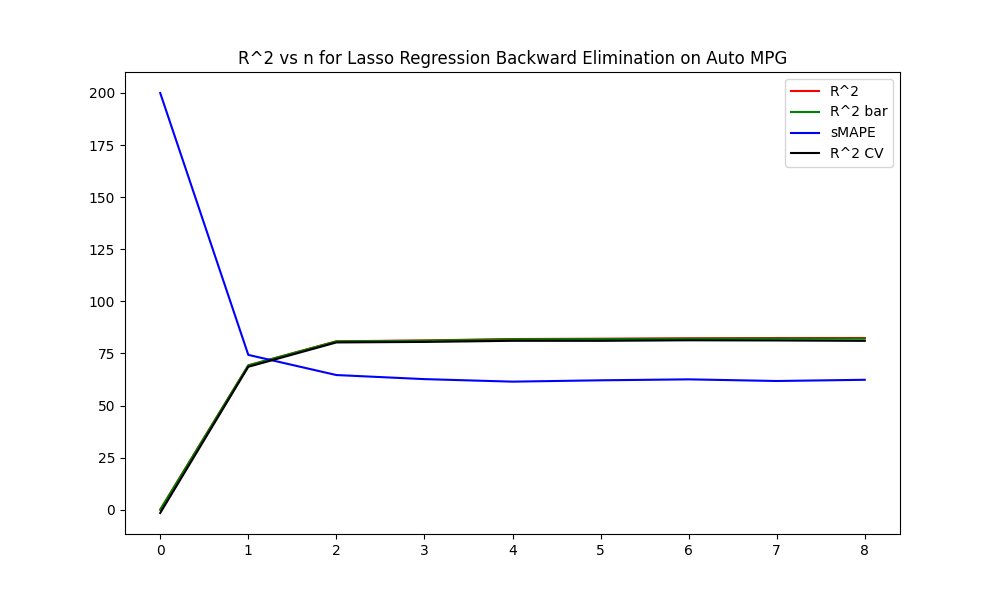
\includegraphics[width=\textwidth]{../Auto_MPG_Statsmodels_Plots/Statsmodels_Lasso_rSq_Backward.png}
     \end{subfigure}
     \hfill
     \begin{subfigure}[b]{0.49\textwidth}
         \centering
         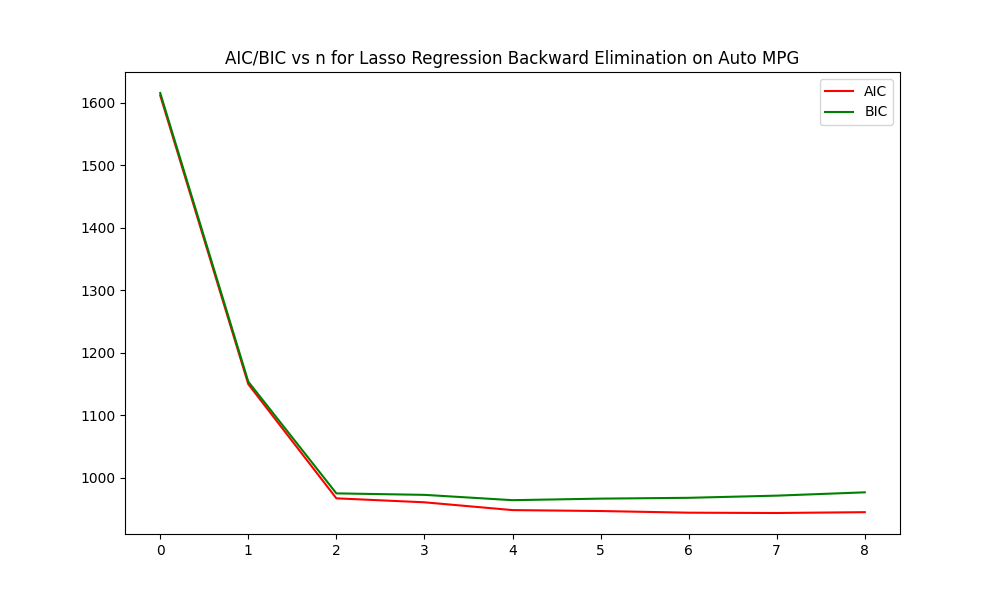
\includegraphics[width=\textwidth]{../Auto_MPG_Statsmodels_Plots/Statsmodels_Lasso_AIC_BIC_Backward.png}
     \end{subfigure}
     
     \caption{Auto MPG Lasso Regression Reversed Backward Elimination Quality of Fit Metrics\\ Top Left: Scalation $R^2$, Top Right: Scalation AIC/BIC\\ Bottom Left: Statsmodels $R^2$, Bottom Right: Statsmodels AIC/BIC}
     \label{fig:Auto MPG Lasso Regression Reversed Backward Elimination Quality of Fit Metrics}
\end{figure}

Scalation Stepwise Selection: displacement, weight, origin 2, modelyear, cylinders, acceleration, horsepower

Statsmodels Stepwise Selection: Null, weight, model year, origin 3, origin 2, displacement, horsepower, cylinders

\begin{figure}[H]
     \centering
     \captionsetup{justification=centering}
     % First Row
     \begin{subfigure}[b]{0.4\textwidth}
         \centering
         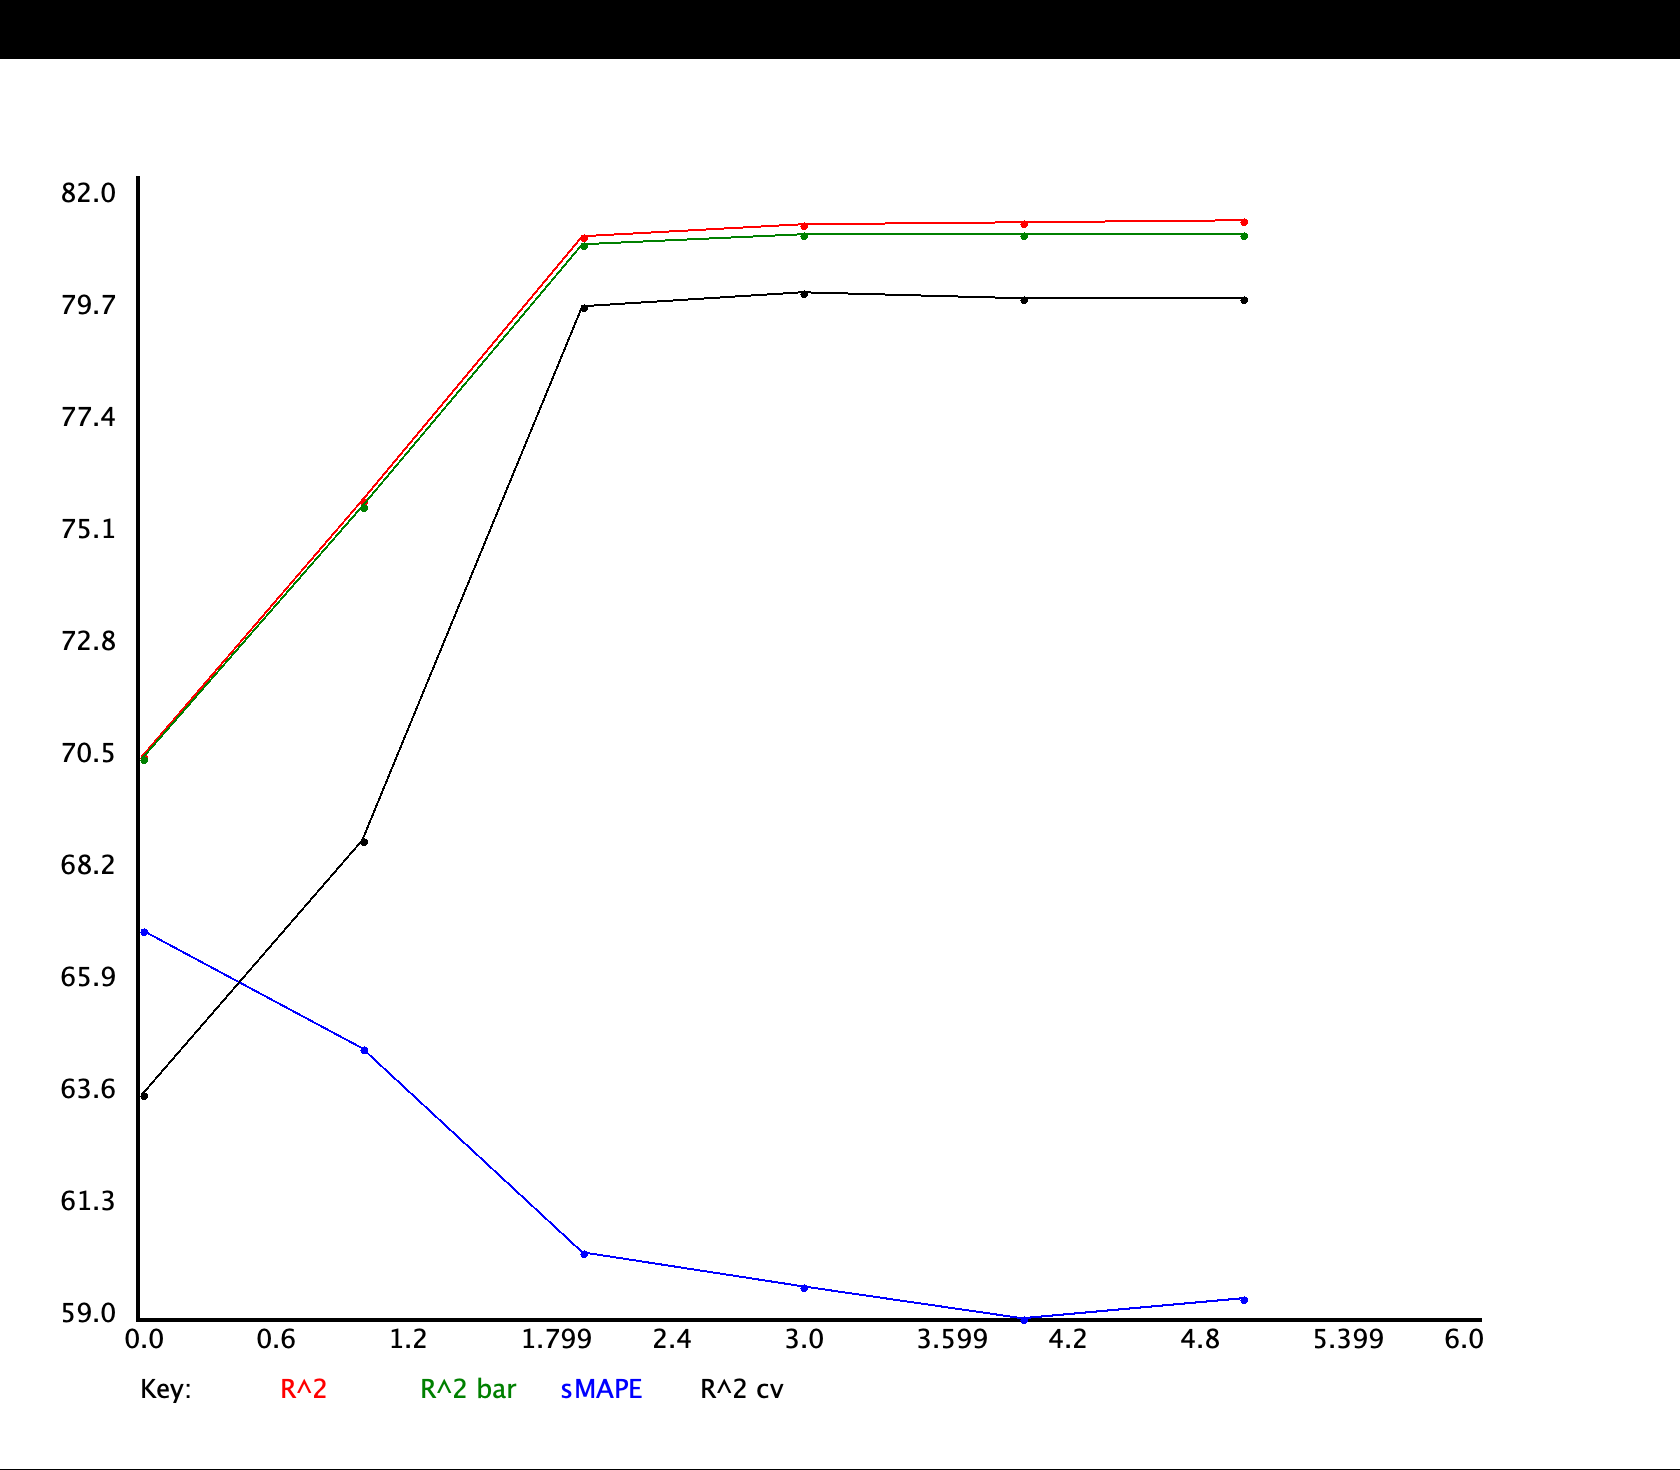
\includegraphics[width=\textwidth]{../Auto_MPG_Scalation_Plots/Scalation_Lasso_rSq_Stepwise.png}
     \end{subfigure}
     \hfill
     \begin{subfigure}[b]{0.4\textwidth}
         \centering
         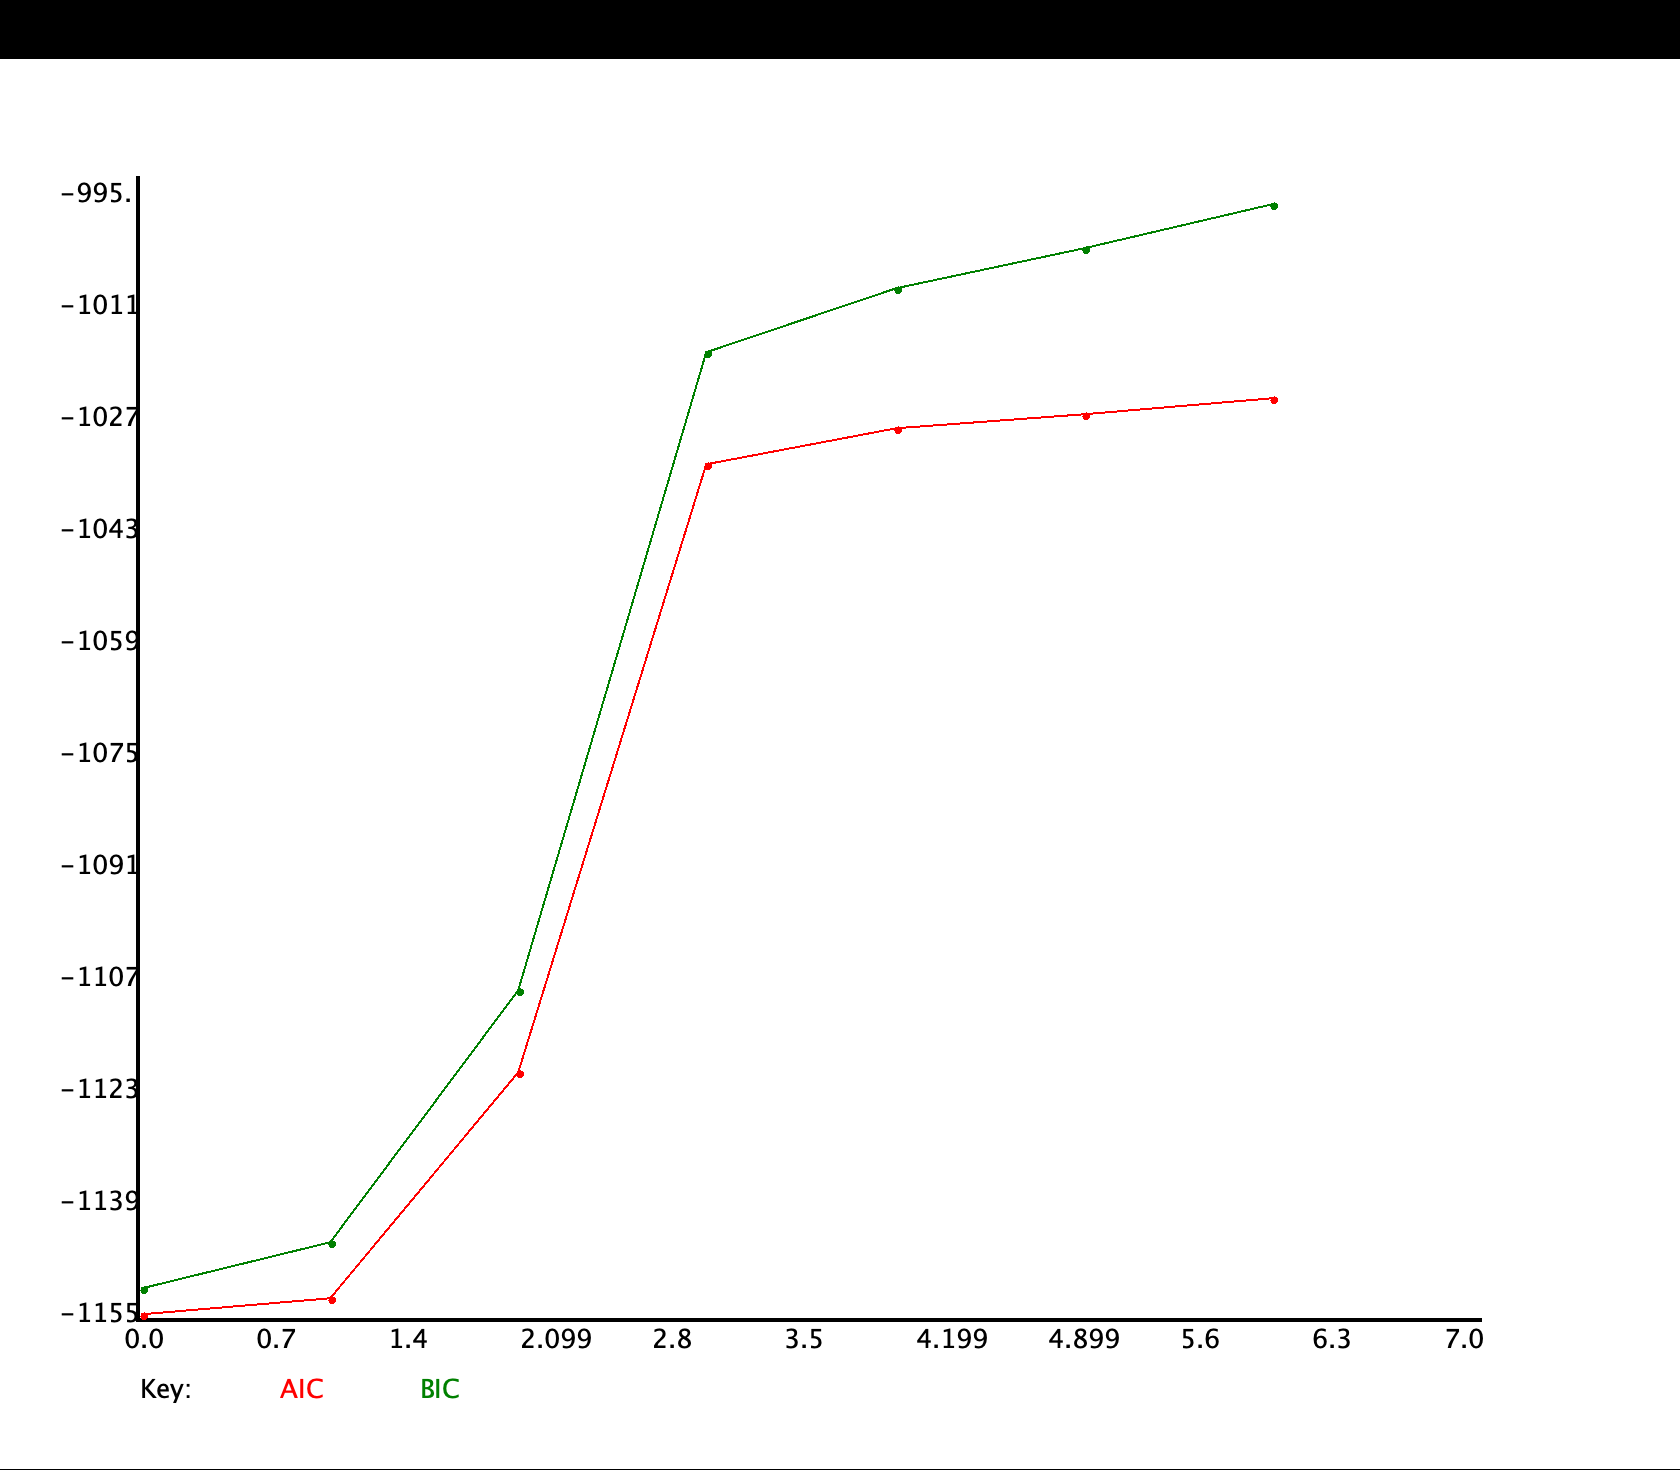
\includegraphics[width=\textwidth]{../Auto_MPG_Scalation_Plots/Scalation_Lasso_AIC_BIC_Stepwise.png}
     \end{subfigure}

     \vspace{10pt} % Add some vertical spacing between rows

     % Second Row
     \begin{subfigure}[b]{0.49\textwidth}
         \centering
         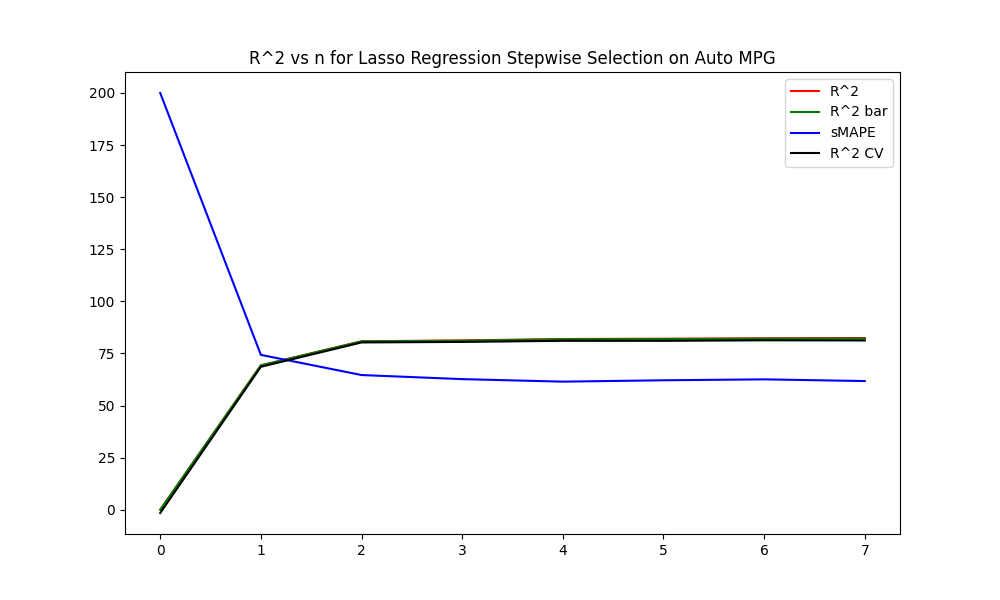
\includegraphics[width=\textwidth]{../Auto_MPG_Statsmodels_Plots/Statsmodels_Lasso_rSq_Stepwise.png}
     \end{subfigure}
     \hfill
     \begin{subfigure}[b]{0.49\textwidth}
         \centering
         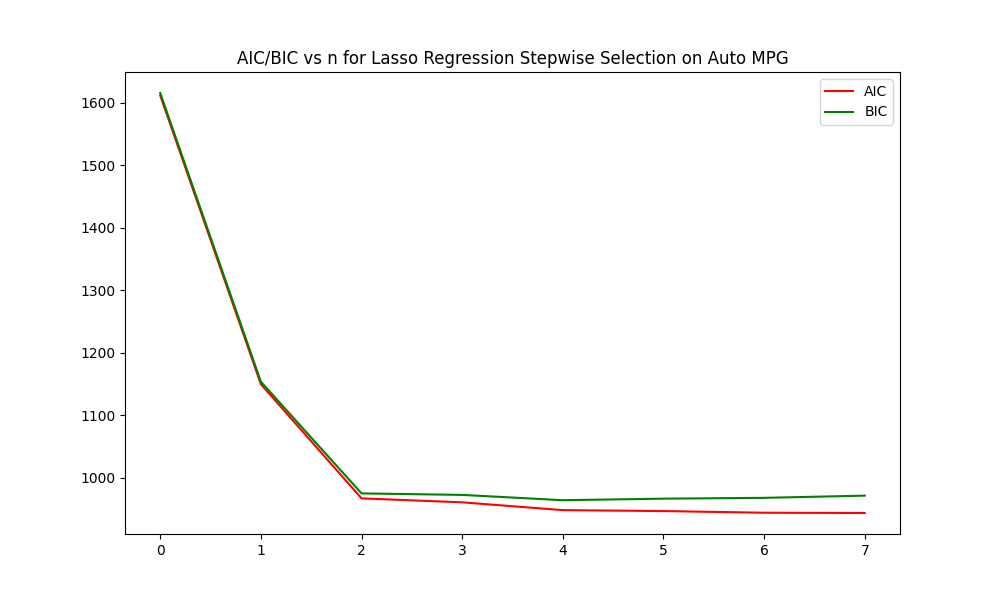
\includegraphics[width=\textwidth]{../Auto_MPG_Statsmodels_Plots/Statsmodels_Lasso_AIC_BIC_Stepwise.png}
     \end{subfigure}
     
     \caption{Auto MPG Lasso Regression Stepwise Selection Quality of Fit Metrics\\ Top Left: Scalation $R^2$, Top Right: Scalation AIC/BIC\\ Bottom Left: Statsmodels $R^2$, Bottom Right: Statsmodels AIC/BIC}
     \label{fig:Auto MPG Lasso Regression Stepwise Selection Quality of Fit Metrics}
\end{figure}

\subsection{Sqrt Transformation}

\subsubsection{Quality of Fit}

\begin{figure}[H]
     \centering
     \captionsetup{justification=centering}
     % First Row
     \begin{subfigure}[b]{0.4\textwidth}
         \centering
         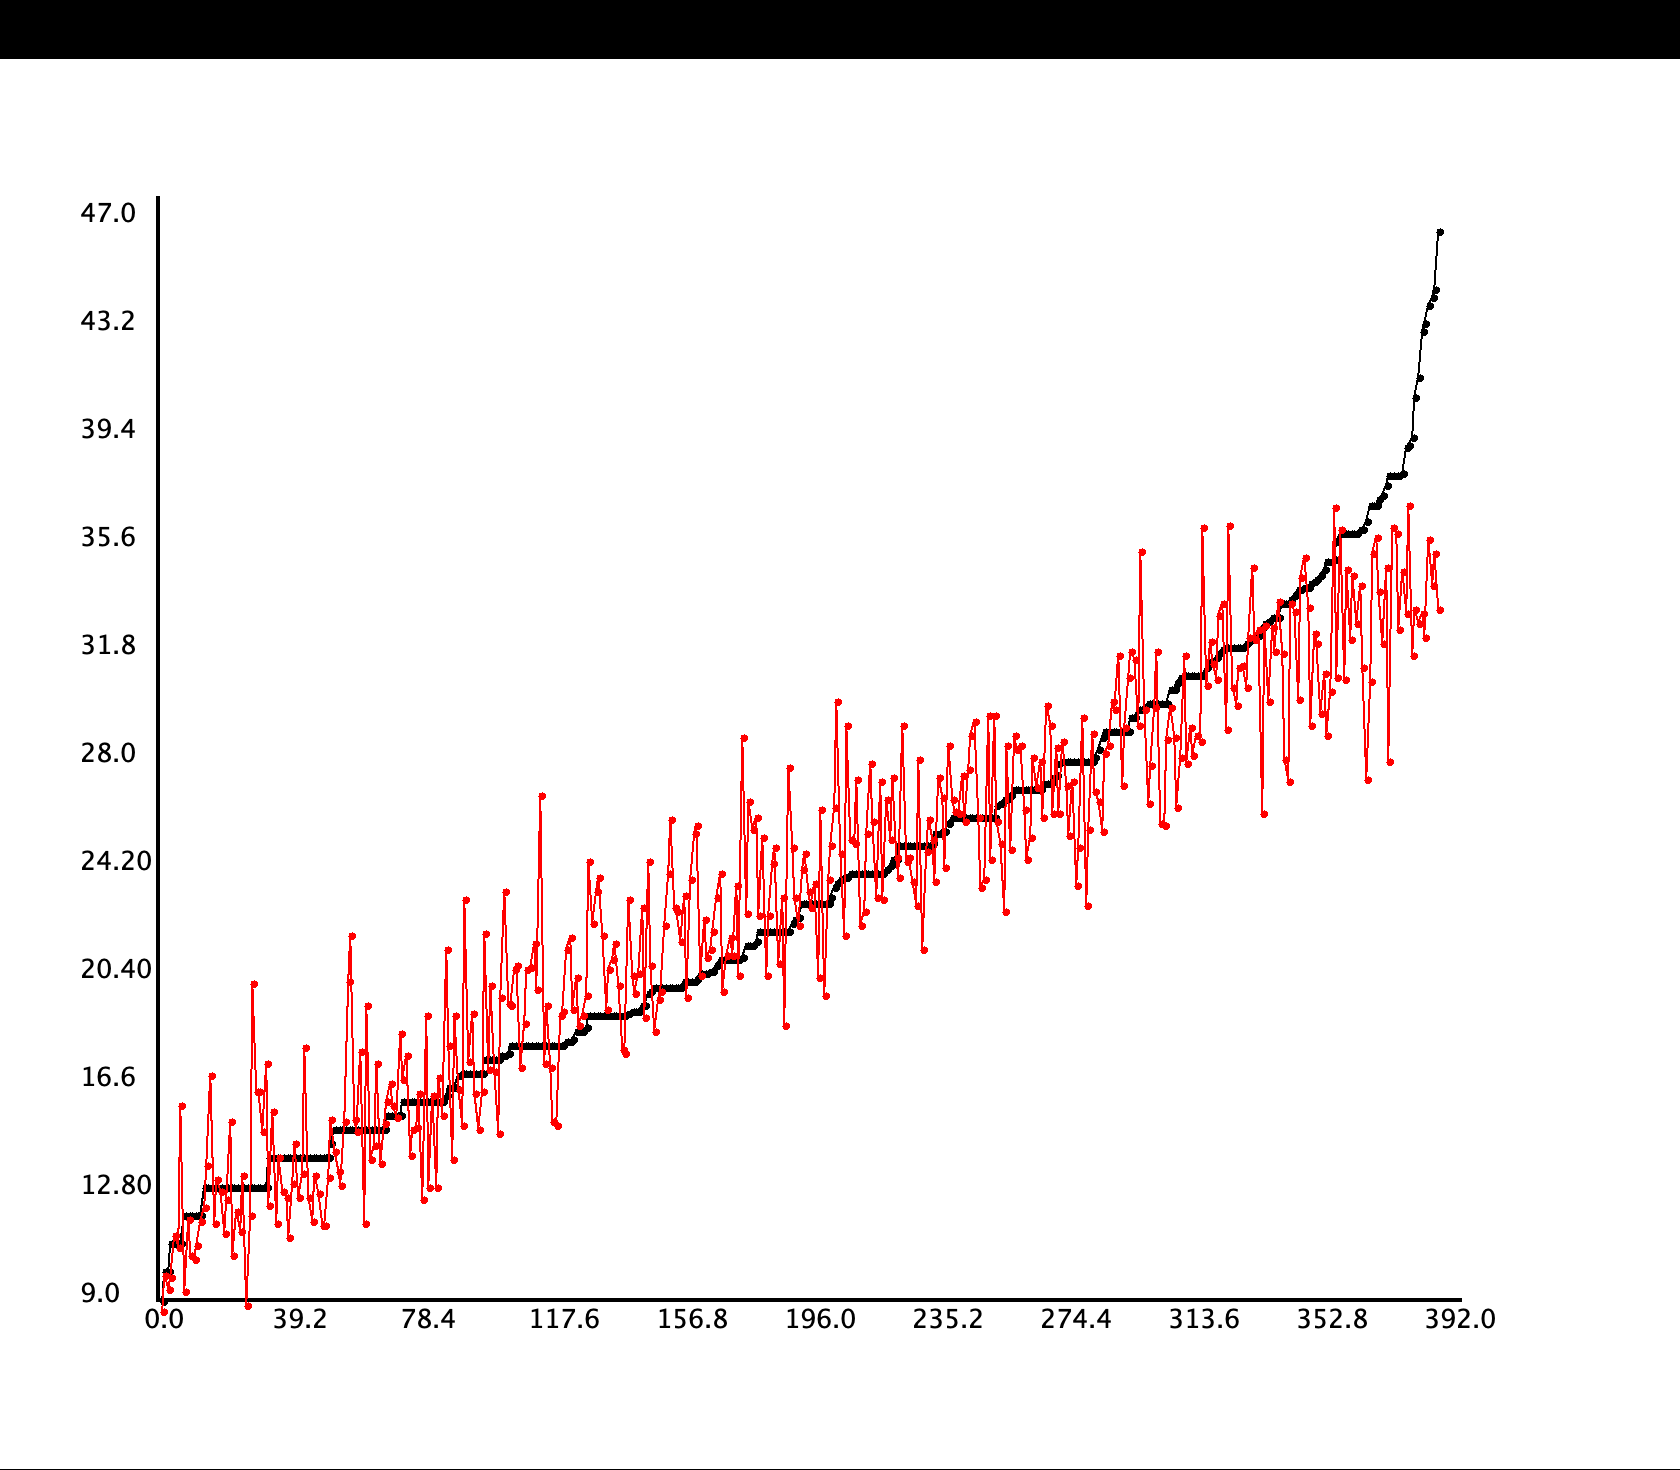
\includegraphics[width=\textwidth]{../Auto_MPG_Scalation_Plots/Scalation_Sqrt_In_Sample.png}
     \end{subfigure}
     \hfill
     \begin{subfigure}[b]{0.4\textwidth}
         \centering
         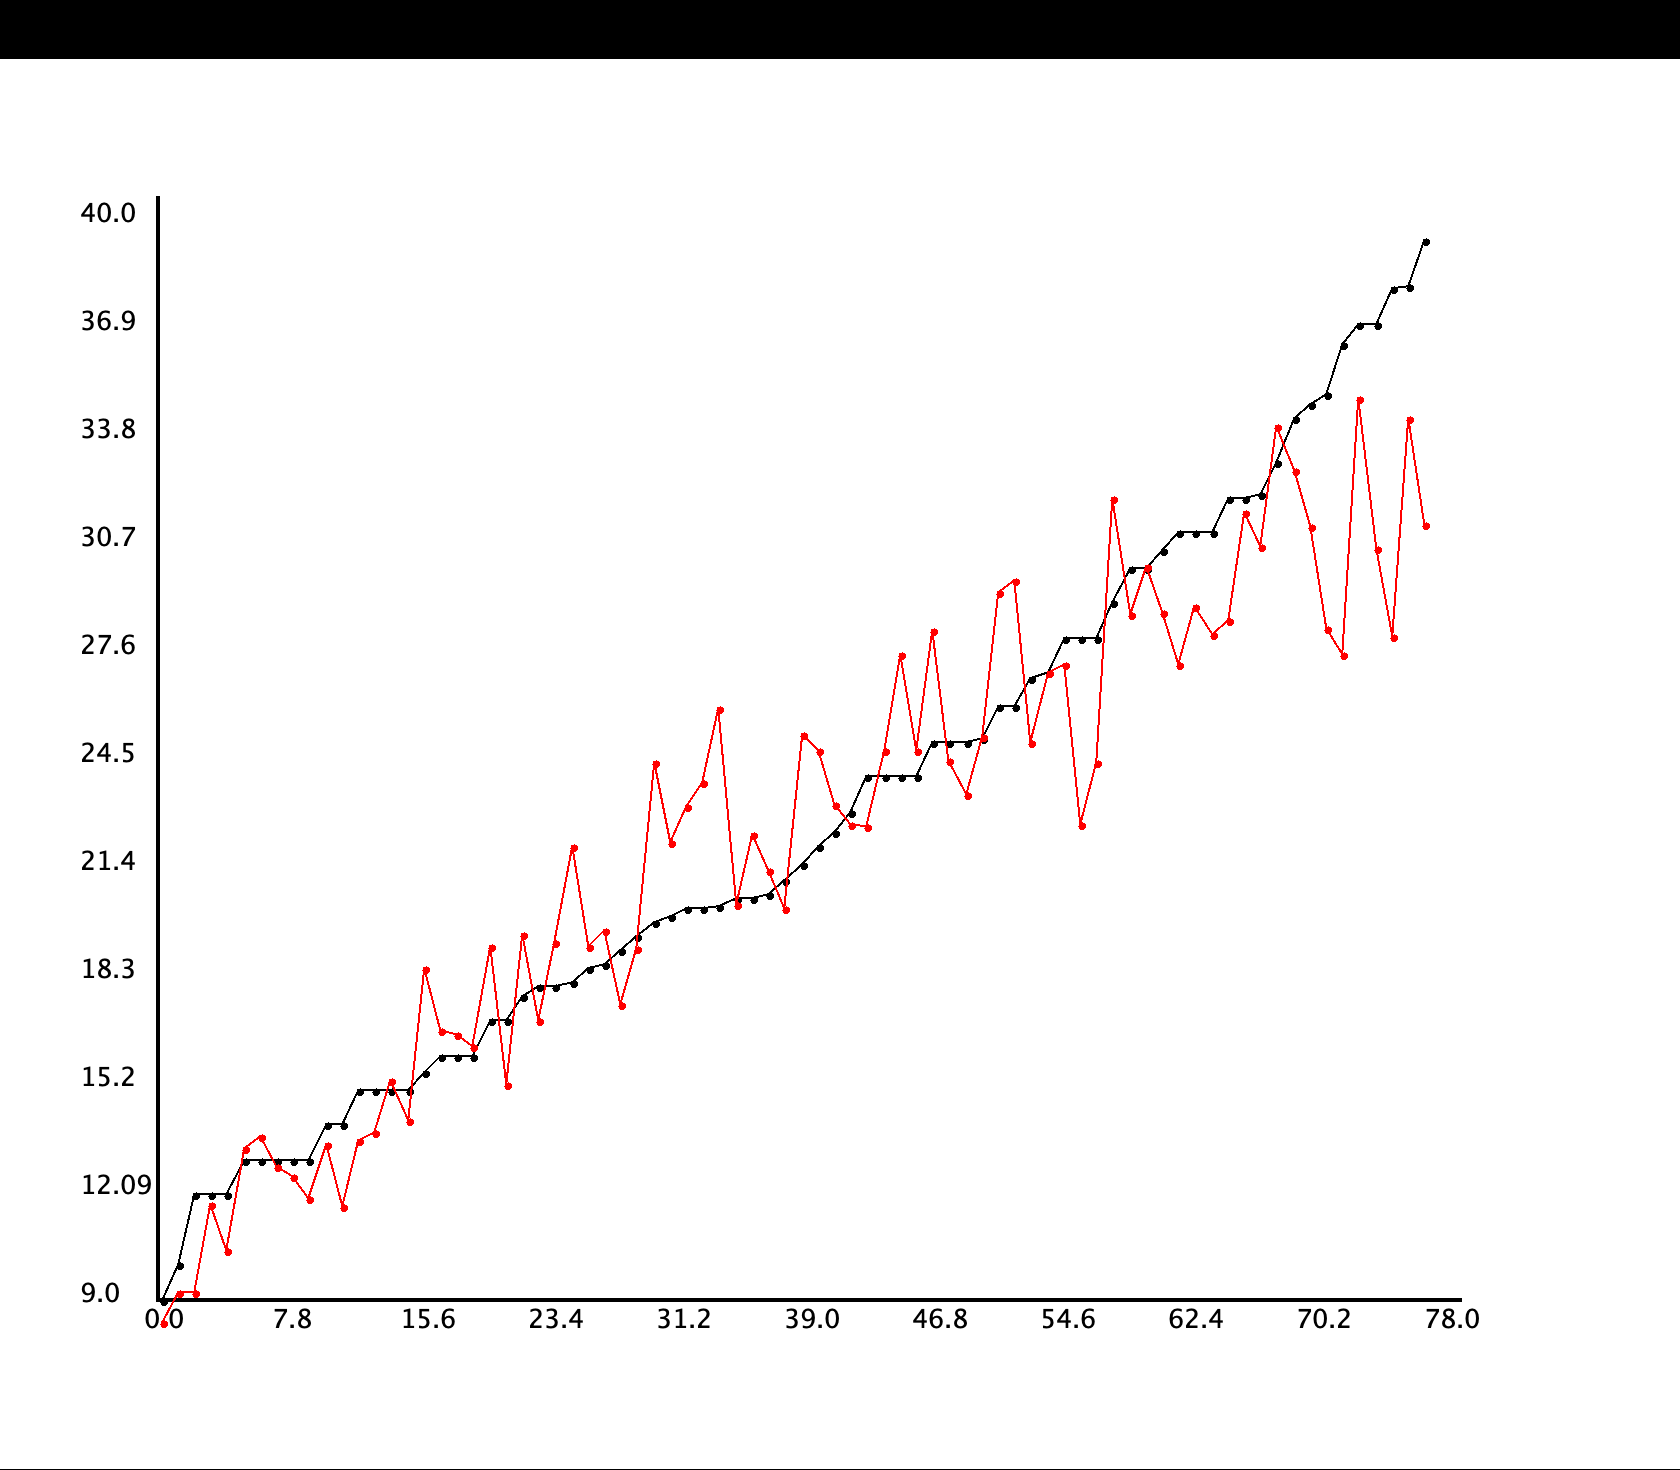
\includegraphics[width=\textwidth]{../Auto_MPG_Scalation_Plots/Scalation_Sqrt_80_20.png}
     \end{subfigure}

     \vspace{10pt} % Add some vertical spacing between rows

     % Second Row
     \begin{subfigure}[b]{0.49\textwidth}
         \centering
         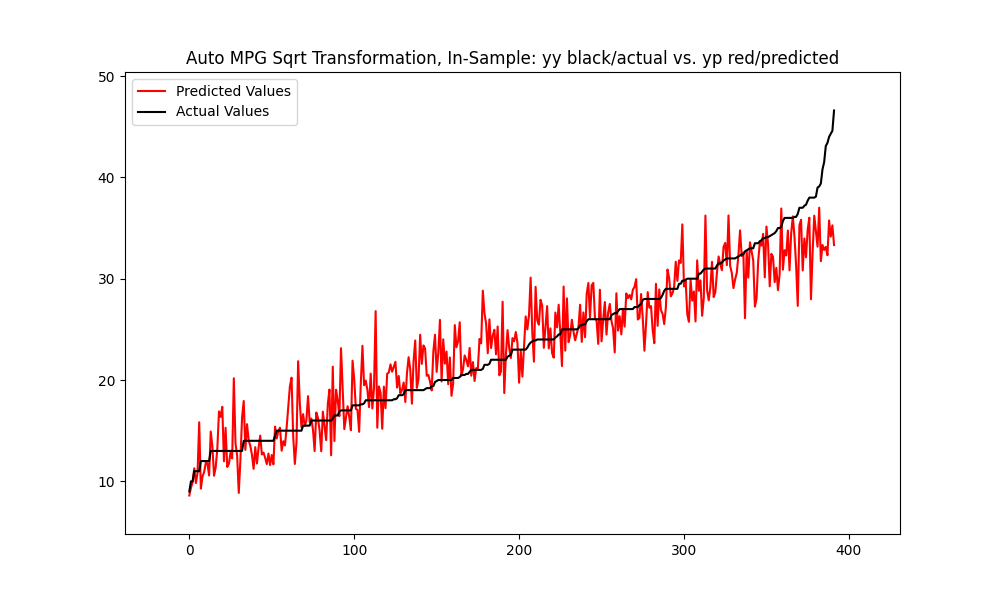
\includegraphics[width=\textwidth]{../Auto_MPG_Statsmodels_Plots/Statsmodels_Sqrt_In_Sample.png}
     \end{subfigure}
     \hfill
     \begin{subfigure}[b]{0.49\textwidth}
         \centering
         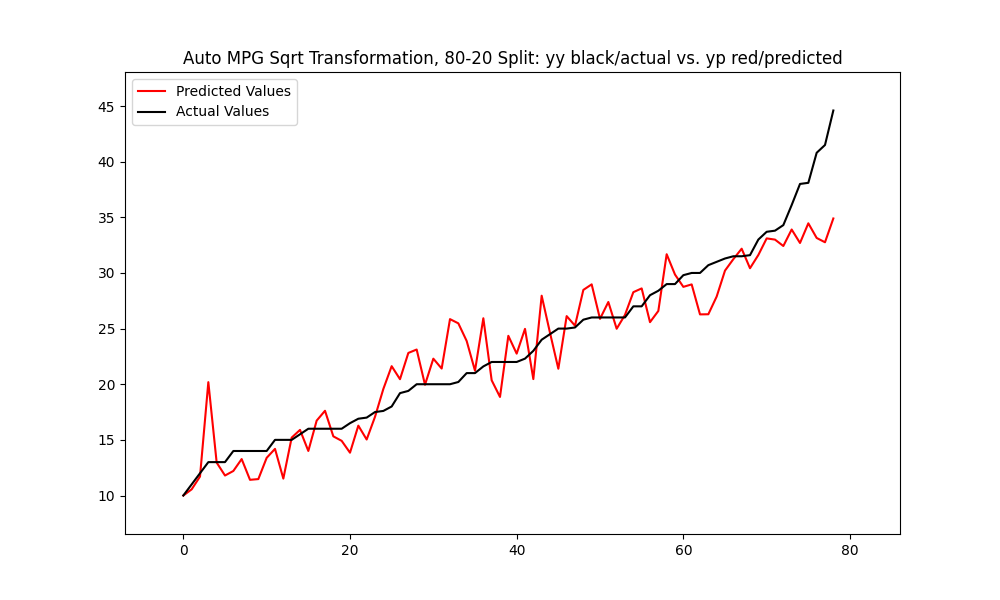
\includegraphics[width=\textwidth]{../Auto_MPG_Statsmodels_Plots/Statsmodels_Sqrt_80_20.png}
     \end{subfigure}
     
     \caption{Auto MPG Sqrt Transformation Plots\\ Top Left: Scalation In-Sample, Top Right: Scalation Out-of-Sample\\ Bottom Left: Statsmodels In-Sample, Bottom Right: Statsmodels Out-of-Sample\\ black: actual y-values, red: predicted y-values}
     \label{fig:Auto MPG Sqrt Transformation Plots}
\end{figure}

\begin{table}[H]
\centering
\caption{Scalation - Auto MPG Sqrt Transformation}
\label{tab:Scalation - Auto MPG Sqrt Transformation}
\begin{tabular}{|c|c|c|} \hline 
Metric & In-Sample & 80-20 Split \\ \hline \hline 
rSq &0.847208 & 0.853580 \\ \hline 
rSqBar &0.844016 &      0.850521 \\ \hline 
sst &23819.0 &  4731.23 \\ \hline 
sse &3639.36 &  692.750 \\ \hline 
sde &3.04951 &  2.95717 \\ \hline 
mse0 &9.28408 & 8.88140 \\ \hline 
rmse &3.04698 & 2.98017 \\ \hline 
mae &2.25769 &  2.15980 \\ \hline 
smape &9.80011 &        9.16865 \\ \hline 
m &392.000 &    78.0000 \\ \hline 
dfr &8.00000 &  8.00000 \\ \hline 
df &383.000 &   383.000 \\ \hline 
fStat &265.459 &        279.094 \\ \hline 
aic &-974.971 & -177.868 \\ \hline 
bic &-939.230 & -156.657 \\ \hline 
\end{tabular}
\end{table}

\begin{table}[H]
\centering
\caption{Statsmodels - Auto MPG Sqrt Transformation}
\label{tab:Statsmodels - Auto MPG Sqrt Transformation}
\begin{tabular}{|c|c|c|}\hline
Metric & In-Sample & 80-20 Split \\ \hline \hline
rSq & 0.8584 & 0.8630 \\ \hline
rSqBar & 0.8554 & 0.8473 \\ \hline
sst & 252.1610 & 4910.2699 \\ \hline
sse & 35.7086 & 672.9259 \\ \hline
sde & 0.3053 & 3.1005 \\ \hline
mse0 & 0.0932 & 8.5180 \\ \hline
rmse & 0.3053 & 2.9186 \\ \hline
mae & 2.2577 & 2.1439 \\ \hline
smape & 9.8001 & 9.2958 \\ \hline
m & 392.0000 & 79.0000 \\ \hline
dfr & 8.0000 & 9.0000 \\ \hline
df & 383.0000 & 70.0000 \\ \hline
fStat & 290.2003 & 48.9759 \\ \hline
aic & 191.2670 & 187.2328 \\ \hline
bic & 227.0084 & 208.5578 \\ \hline
\end{tabular}
\end{table}

\begin{table}[H]
\centering
\caption{Scalation - Auto MPG Sqrt Transformation CV}
\label{tab:Scalation - Auto MPG Sqrt Transformation CV}
\begin{tabular}{|c|c|c|c|c|c|}\hline
Metric & num folds & min & max & mean & stdev \\ \hline \hline
rSq & 5 & 0.812 & 0.854 & 0.835 & 0.015 \\ \hline
rSqBar & 5 & 0.808 & 0.851 & 0.831 & 0.015 \\ \hline
sst & 5 & 3962.818 & 5671.580 & 4700.481 & 620.767 \\ \hline
sse & 5 & 636.974 & 938.793 & 777.312 & 119.212 \\ \hline
sde & 5 & 2.777 & 3.320 & 3.101 & 0.229 \\ \hline
mse0 & 5 & 8.166 & 12.036 & 9.966 & 1.528 \\ \hline
rmse & 5 & 2.858 & 3.469 & 3.149 & 0.242 \\ \hline
mae & 5 & 2.160 & 2.537 & 2.320 & 0.155 \\ \hline
smape & 5 & 9.169 & 11.184 & 10.048 & 0.760 \\ \hline
m & 5 & 78.000 & 78.000 & 78.000 & 0.000 \\ \hline
dfr & 5 & 8.000 & 8.000 & 8.000 & 0.000 \\ \hline
df & 5 & 383.000 & 383.000 & 383.000 & 0.000 \\ \hline
fStat & 5 & 207.046 & 279.094 & 243.316 & 25.794 \\ \hline
aic & 5 & -192.118 & -174.637 & -182.765 & 6.905 \\ \hline
bic & 5 & -170.908 & -153.427 & -161.555 & 6.905 \\ \hline
\end{tabular}
\end{table}

\begin{table}[H]
\centering
\caption{Statsmodels - Auto MPG Sqrt Transformation CV}
\label{tab:Statsmodels - Auto MPG Sqrt Transformation CV}
\begin{tabular}{|c|c|c|c|c|c|}\hline
Metric & num folds & min & max & mean & stdev \\ \hline \hline
rSq & 5 & 0.7604 & 0.8683 & 0.8327 & 0.0385 \\ \hline
rSqBar & 5 & 0.7327 & 0.8530 & 0.8134 & 0.0430 \\ \hline
sst & 5 & 3880.9704 & 5093.9237 & 4721.1782 & 441.3031 \\ \hline
sse & 5 & 671.1031 & 929.7604 & 773.6072 & 96.8753 \\ \hline
sde & 5 & 3.1005 & 3.6708 & 3.3326 & 0.2125 \\ \hline
mse0 & 5 & 8.5180 & 11.9200 & 9.8710 & 1.2649 \\ \hline
rmse & 5 & 2.9186 & 3.4525 & 3.1355 & 0.1993 \\ \hline
mae & 5 & 2.1198 & 2.7244 & 2.3318 & 0.2195 \\ \hline
smape & 5 & 9.1432 & 12.5052 & 10.1388 & 1.2552 \\ \hline
m & 5 & 78.0000 & 79.0000 & 78.4000 & 0.4899 \\ \hline
dfr & 5 & 9.0000 & 9.0000 & 9.0000 & 0.0000 \\ \hline
df & 5 & 69.0000 & 70.0000 & 69.4000 & 0.4899 \\ \hline
fStat & 5 & 24.3352 & 50.5262 & 40.5073 & 9.3418 \\ \hline
aic & 5 & 185.8727 & 211.3010 & 196.8483 & 9.4236 \\ \hline
bic & 5 & 207.0831 & 232.5114 & 218.1045 & 9.4046 \\ \hline
\end{tabular}
\end{table}

\subsubsection{Feature Selection}

Scalation Forward Selection: intercept, origin 2, modelyear, acceleration, origin 3, horsepower, displacement, cylinders, weight

Statsmodels Forward Selection: intercept, weight, model year, origin 2, origin 3, horsepower, displacement, acceleration, cylinders

\begin{figure}[H]
     \centering
     \captionsetup{justification=centering}
     % First Row
     \begin{subfigure}[b]{0.4\textwidth}
         \centering
         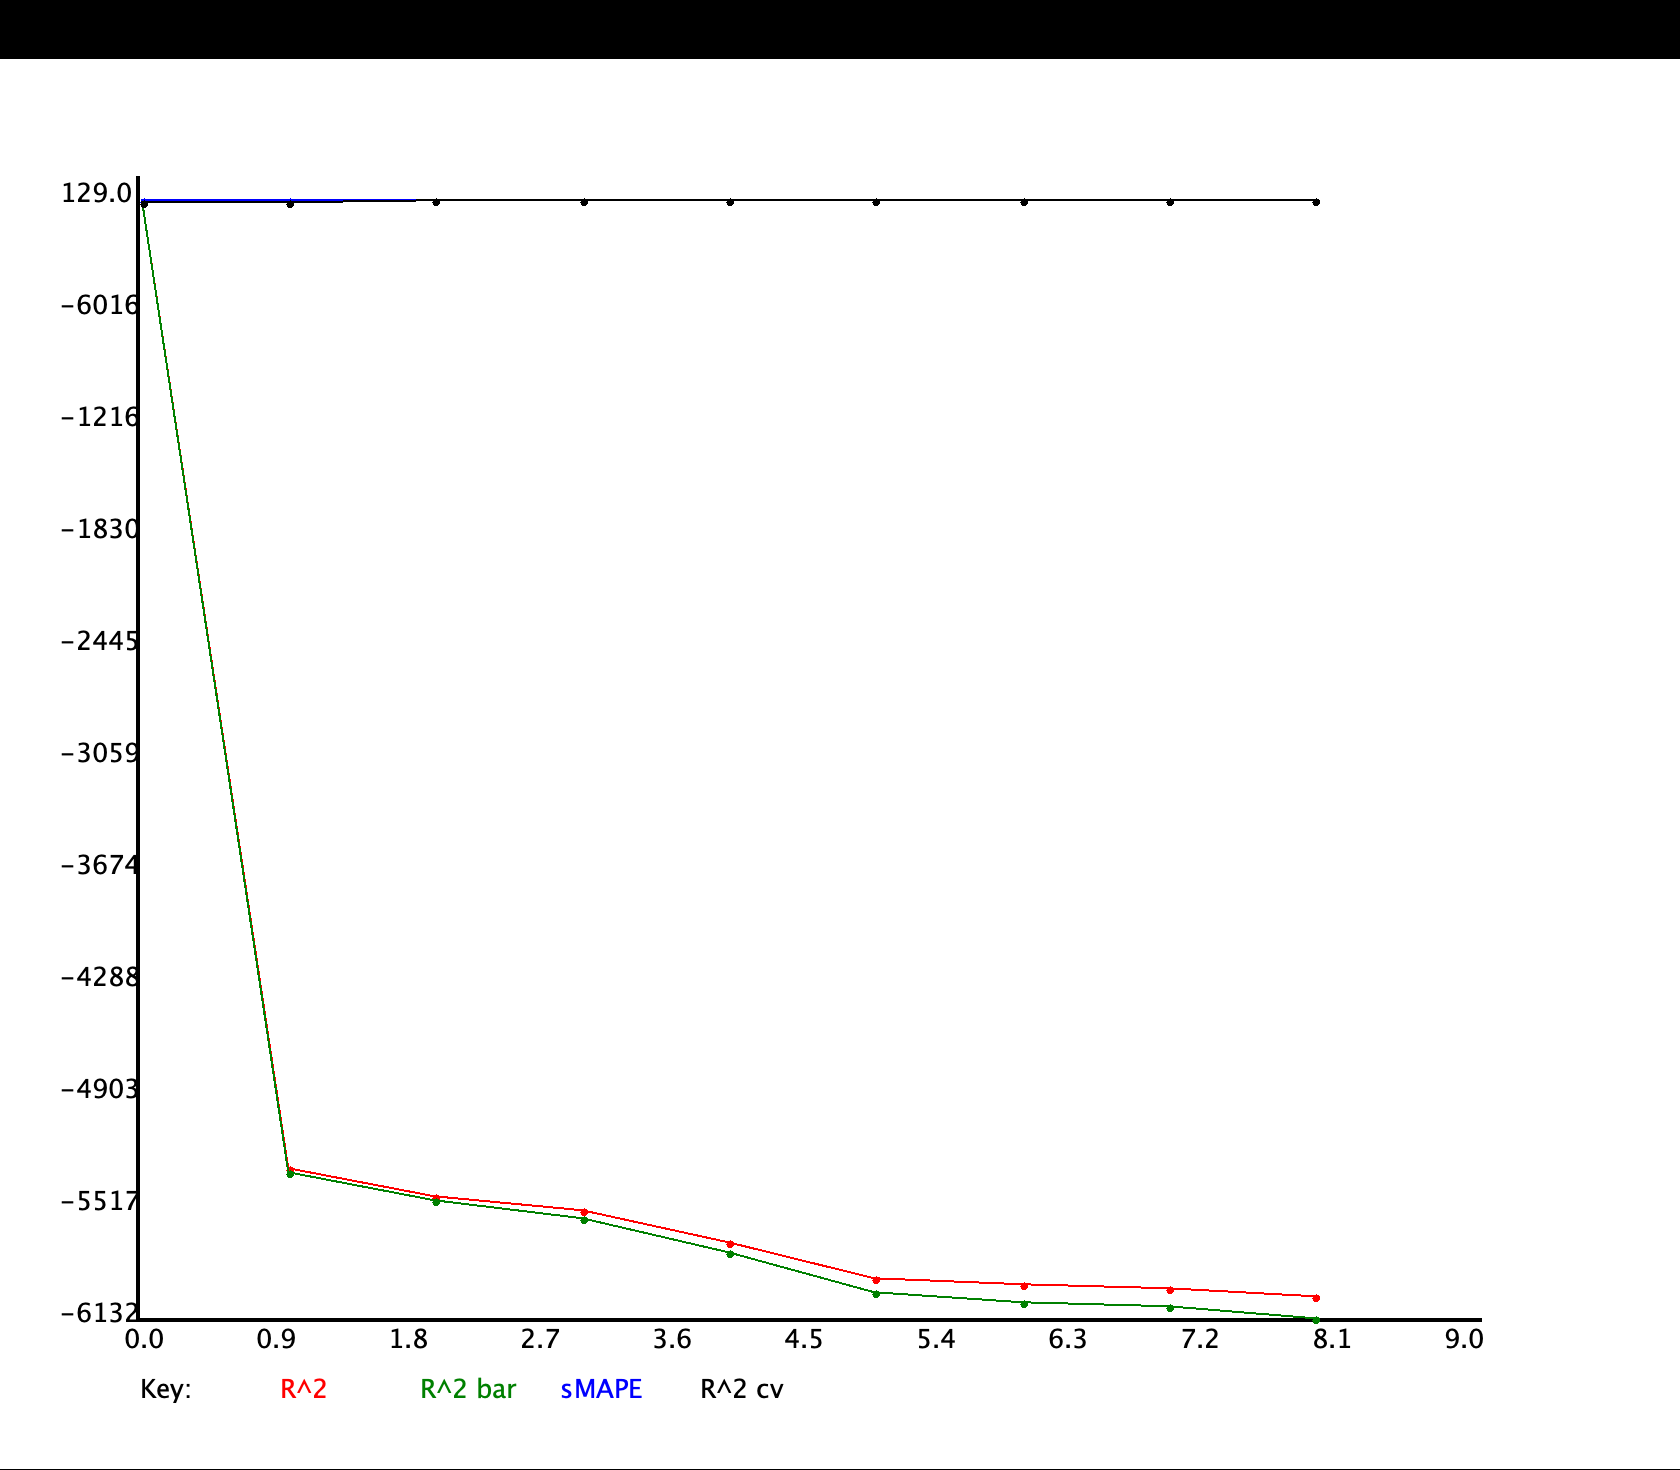
\includegraphics[width=\textwidth]{../Auto_MPG_Scalation_Plots/Scalation_Sqrt_rSq_Forward.png}
     \end{subfigure}
     \hfill
     \begin{subfigure}[b]{0.4\textwidth}
         \centering
         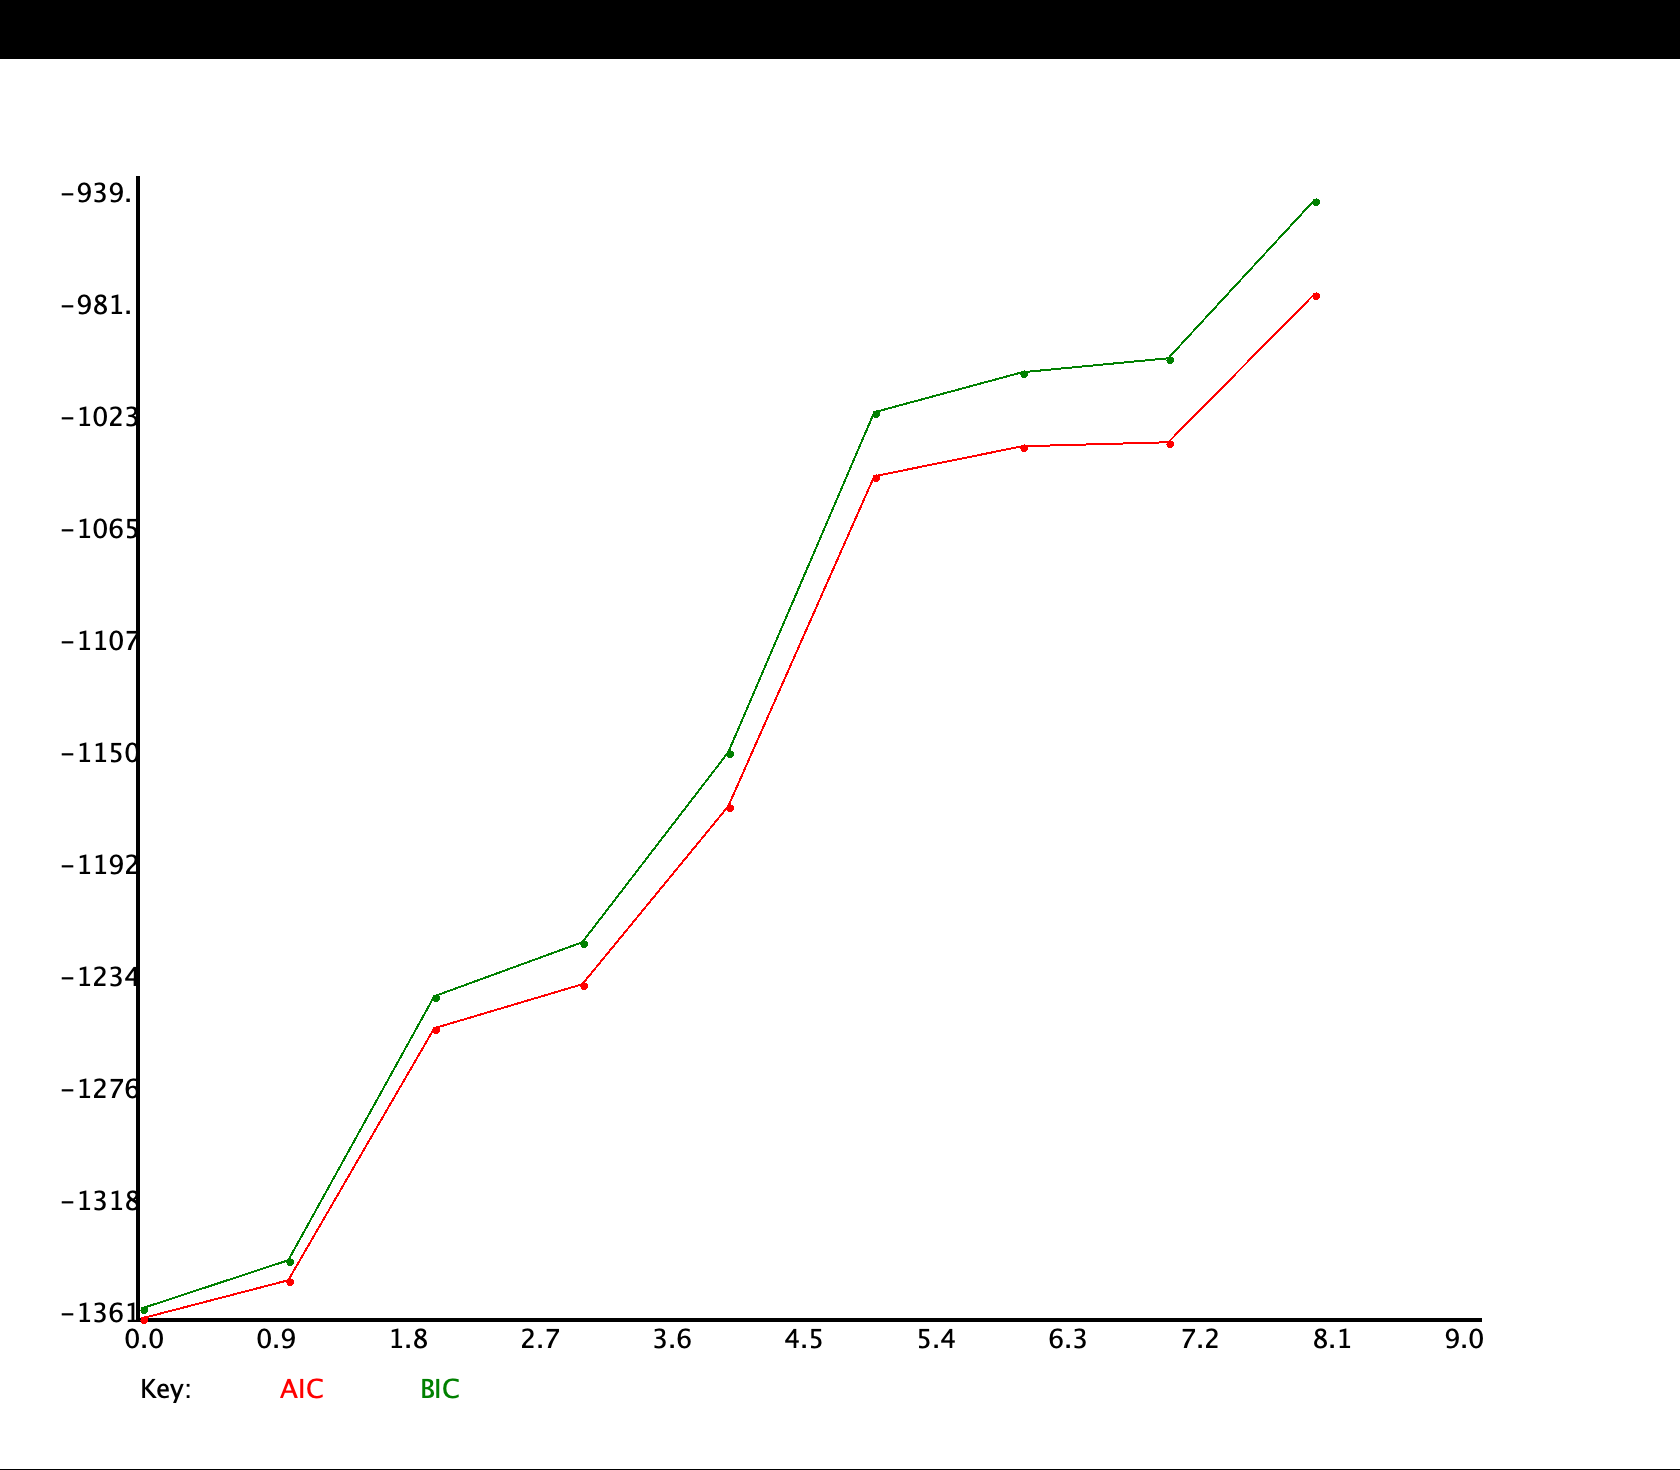
\includegraphics[width=\textwidth]{../Auto_MPG_Scalation_Plots/Scalation_Sqrt_AIC_BIC_Forward.png}
     \end{subfigure}

     \vspace{10pt} % Add some vertical spacing between rows

     % Second Row
     \begin{subfigure}[b]{0.49\textwidth}
         \centering
         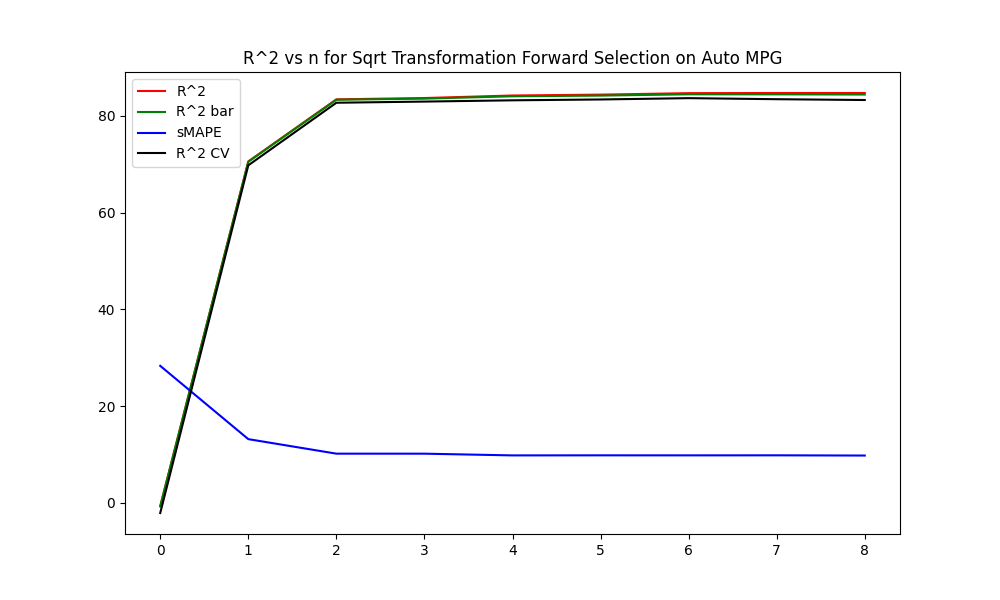
\includegraphics[width=\textwidth]{../Auto_MPG_Statsmodels_Plots/Statsmodels_Sqrt_rSq_Forward.png}
     \end{subfigure}
     \hfill
     \begin{subfigure}[b]{0.49\textwidth}
         \centering
         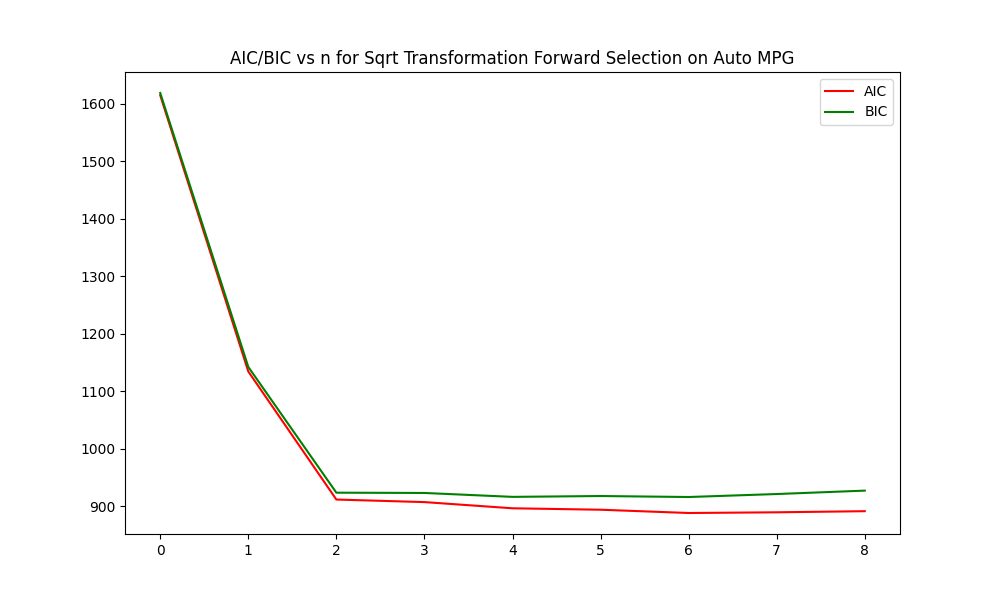
\includegraphics[width=\textwidth]{../Auto_MPG_Statsmodels_Plots/Statsmodels_Sqrt_AIC_BIC_Forward.png}
     \end{subfigure}
     
     \caption{Auto MPG Sqrt Transformation Forward Selection Quality of Fit Metrics\\ Top Left: Scalation $R^2$, Top Right: Scalation AIC/BIC\\ Bottom Left: Statsmodels $R^2$, Bottom Right: Statsmodels AIC/BIC}
     \label{fig:Auto MPG Sqrt Transformation Forward Selection Quality of Fit Metrics}
\end{figure}

Scalation Backward Elimination Reversed: intercept, origin 2, acceleration, origin 3, cylinders, displacement, horsepower, weight, modelyear

Statsmodels Backward Elimination Reversed: intercept, weight, model year, origin 2, origin 3, horsepower, displacement, acceleration, cylinders

\begin{figure}[H]
     \centering
     \captionsetup{justification=centering}
     % First Row
     \begin{subfigure}[b]{0.4\textwidth}
         \centering
         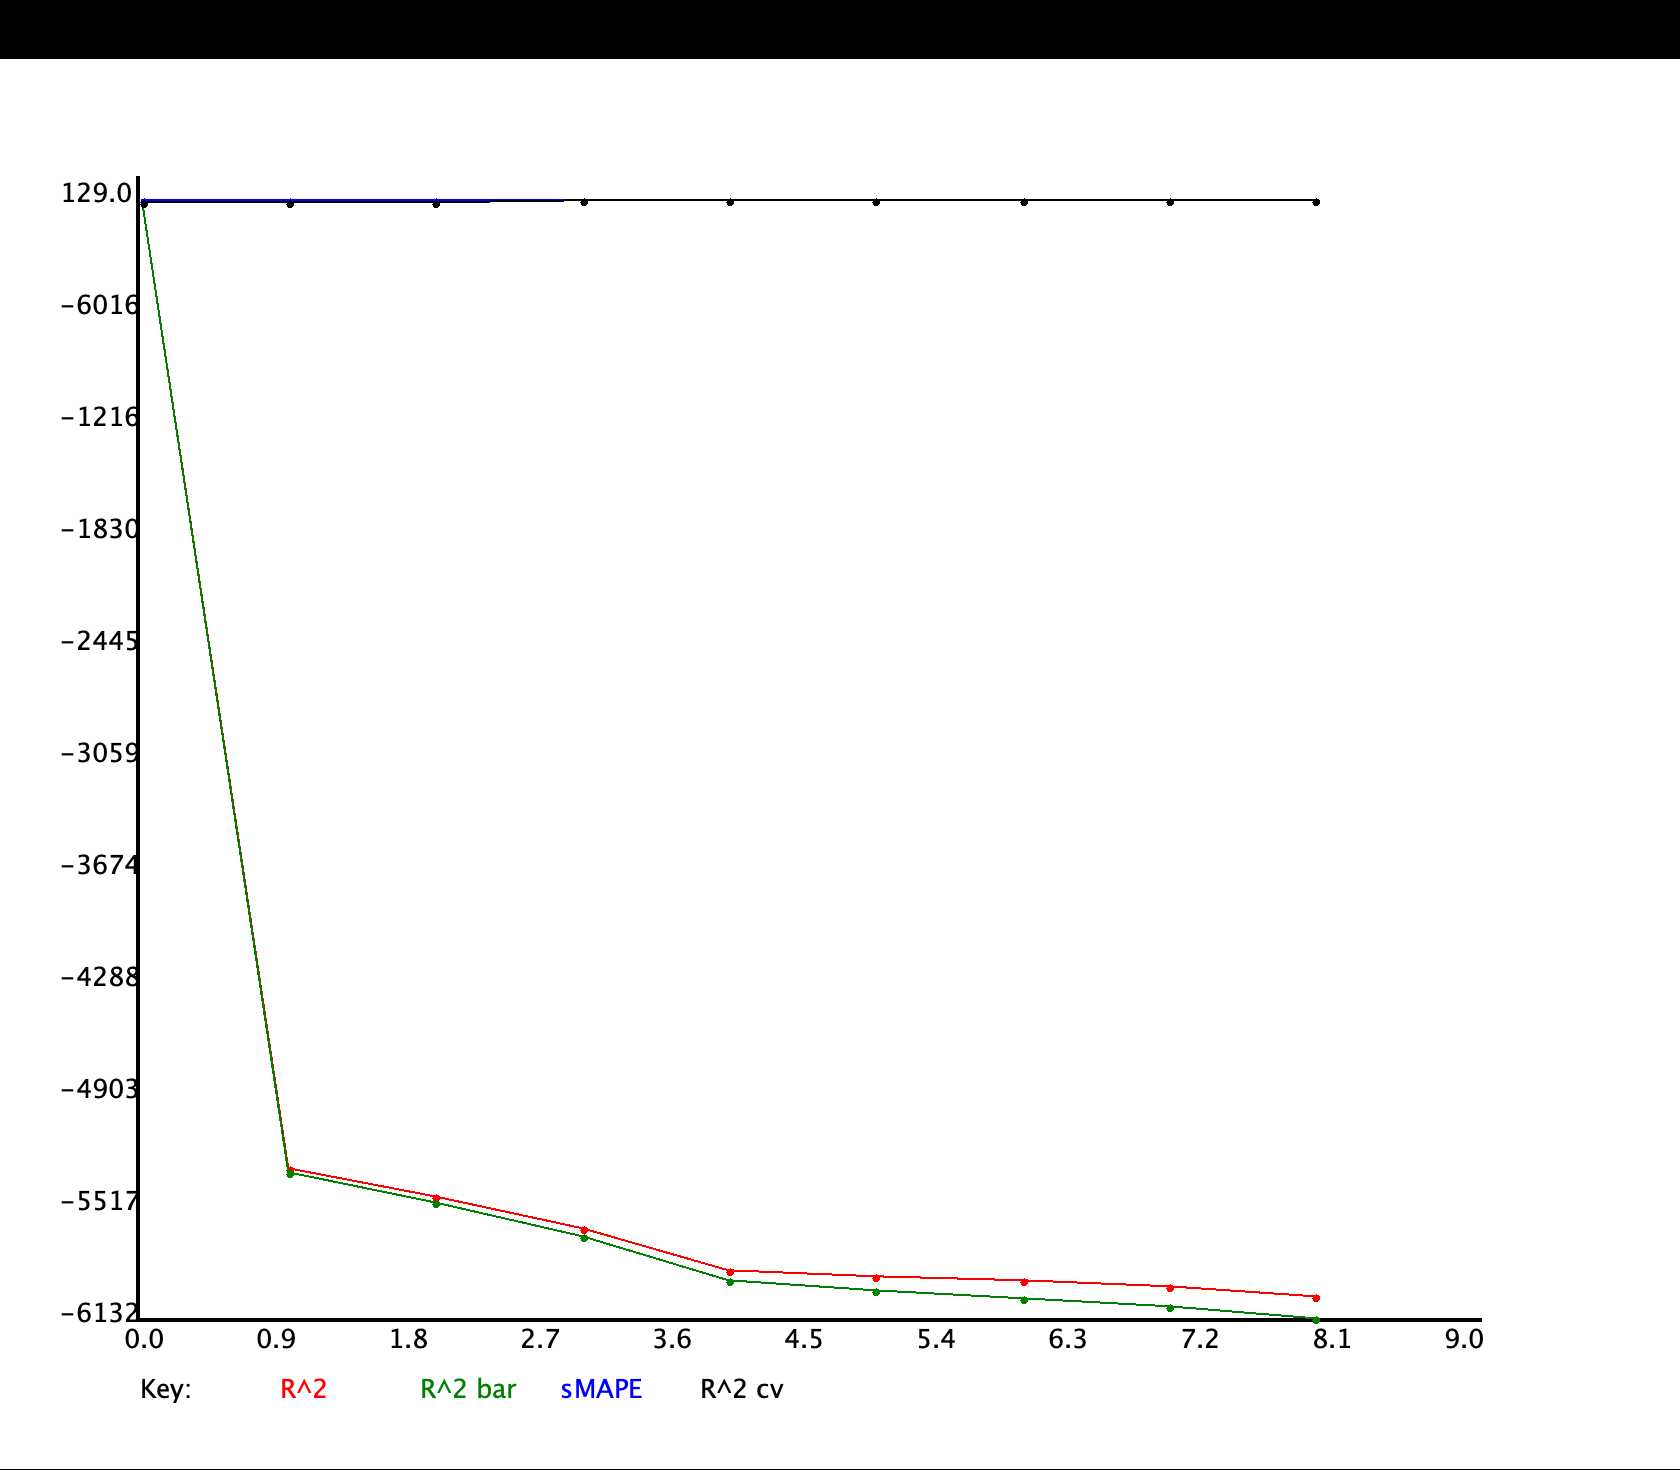
\includegraphics[width=\textwidth]{../Auto_MPG_Scalation_Plots/Scalation_Sqrt_rSq_Backward.png}
     \end{subfigure}
     \hfill
     \begin{subfigure}[b]{0.4\textwidth}
         \centering
         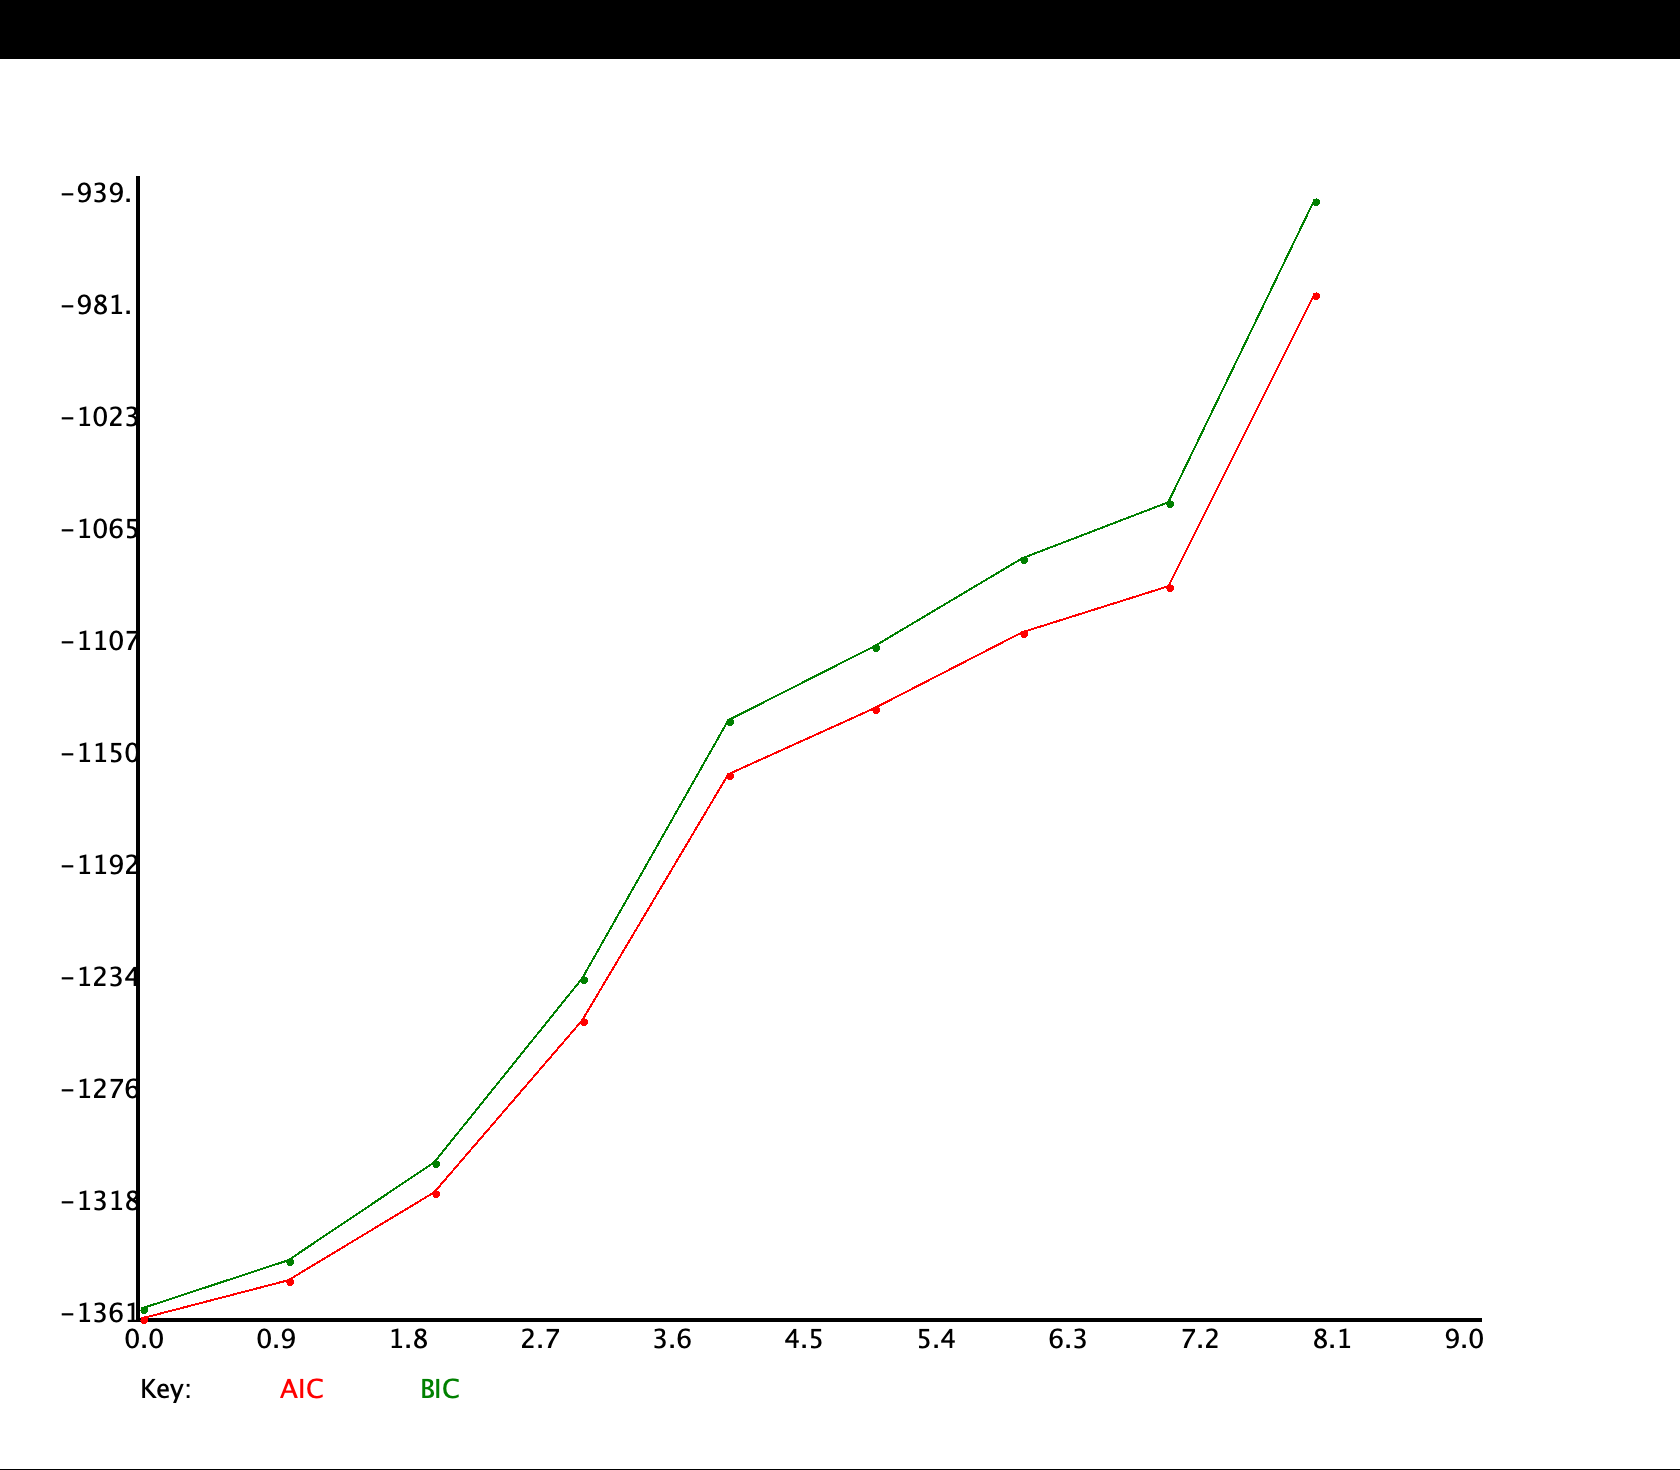
\includegraphics[width=\textwidth]{../Auto_MPG_Scalation_Plots/Scalation_Sqrt_AIC_BIC_Backward.png}
     \end{subfigure}

     \vspace{10pt} % Add some vertical spacing between rows

     % Second Row
     \begin{subfigure}[b]{0.49\textwidth}
         \centering
         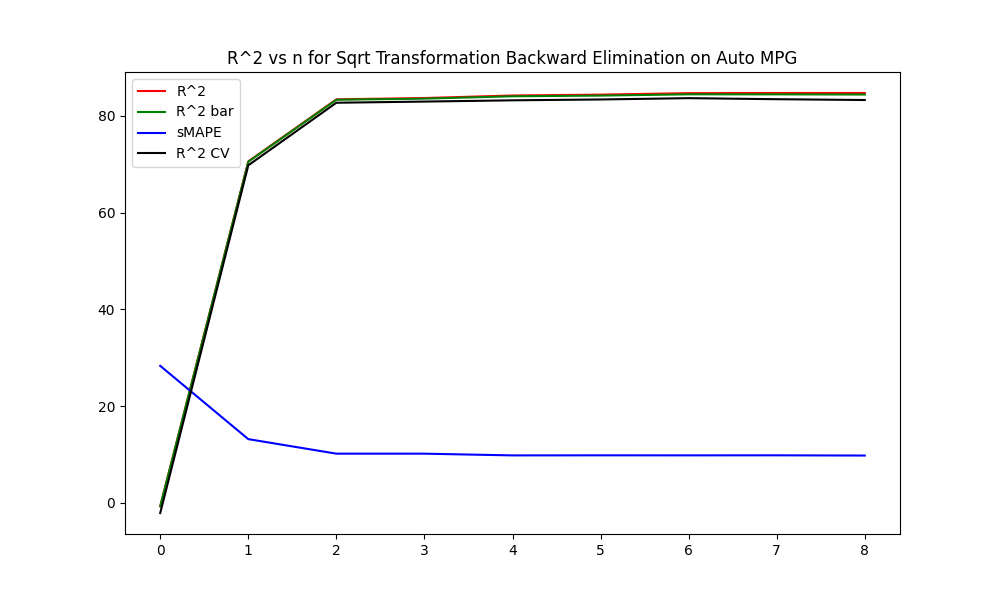
\includegraphics[width=\textwidth]{../Auto_MPG_Statsmodels_Plots/Statsmodels_Sqrt_rSq_Backward.png}
     \end{subfigure}
     \hfill
     \begin{subfigure}[b]{0.49\textwidth}
         \centering
         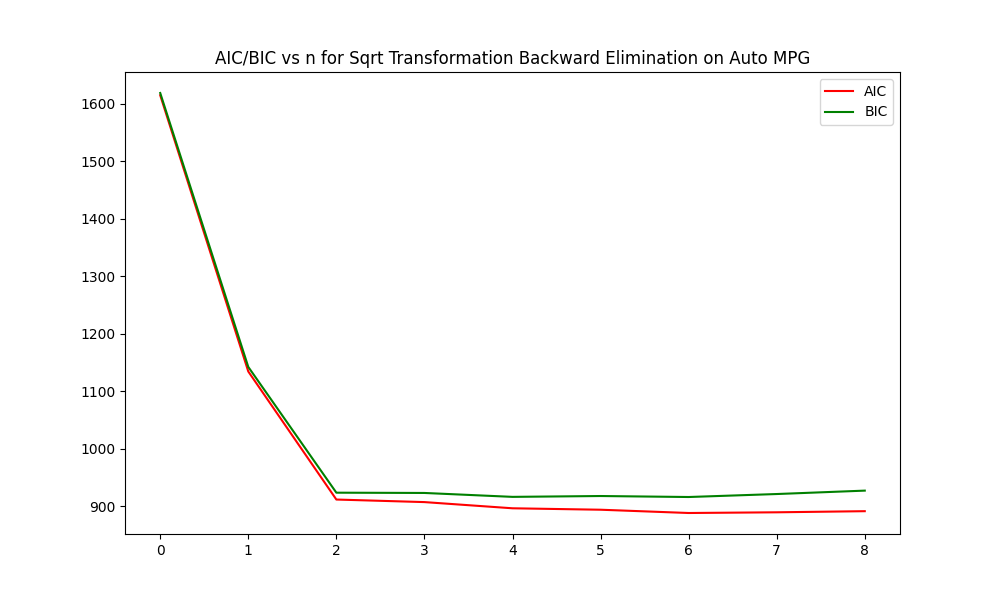
\includegraphics[width=\textwidth]{../Auto_MPG_Statsmodels_Plots/Statsmodels_Sqrt_AIC_BIC_Backward.png}
     \end{subfigure}
     
     \caption{Auto MPG Sqrt Transformation Reversed Backward Elimination Quality of Fit Metrics\\ Top Left: Scalation $R^2$, Top Right: Scalation AIC/BIC\\ Bottom Left: Statsmodels $R^2$, Bottom Right: Statsmodels AIC/BIC}
     \label{fig:Auto MPG Sqrt Transformation Reversed Backward Elimination Quality of Fit Metrics}
\end{figure}

Scalation Stepwise Selection: intercept

Statsmodels Stepwise Selection: intercept, weight, model year, origin 2, origin 3, horsepower, displacement

\begin{figure}[H]
     \centering
     \captionsetup{justification=centering}
%     % First Row
%     \begin{subfigure}[b]{0.4\textwidth}
%         \centering
%         %\includegraphics[width=\textwidth]{../Auto_MPG_Scalation_Plots/Scalation_Sqrt_rSq_Stepwise.png}
%     \end{subfigure}
%     \hfill
%     \begin{subfigure}[b]{0.4\textwidth}
%         \centering
%         %\includegraphics[width=\textwidth]{../Auto_MPG_Scalation_Plots/Scalation_Sqrt_AIC_BIC_Stepwise.png}
%     \end{subfigure}
%
%     \vspace{10pt} % Add some vertical spacing between rows

     % Second Row
     \begin{subfigure}[b]{0.49\textwidth}
         \centering
         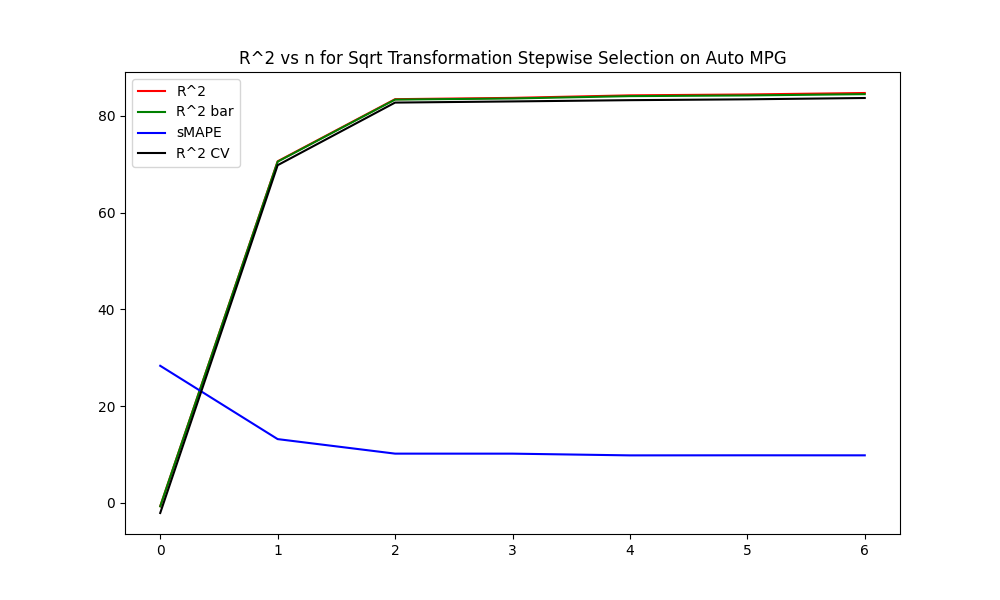
\includegraphics[width=\textwidth]{../Auto_MPG_Statsmodels_Plots/Statsmodels_Sqrt_rSq_Stepwise.png}
     \end{subfigure}
     \hfill
     \begin{subfigure}[b]{0.49\textwidth}
         \centering
         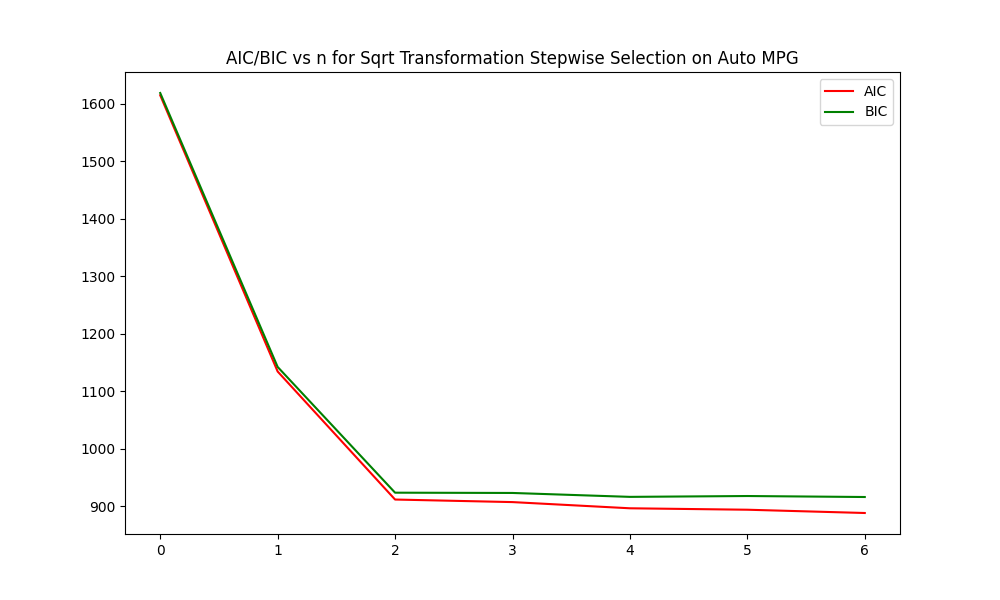
\includegraphics[width=\textwidth]{../Auto_MPG_Statsmodels_Plots/Statsmodels_Sqrt_AIC_BIC_Stepwise.png}
     \end{subfigure}
     
     \caption{Auto MPG Sqrt Transformation Stepwise Selection Quality of Fit Metrics\\ Left: Statsmodels $R^2$, Right: Statsmodels AIC/BIC}
     \label{fig:Auto MPG Sqrt Transformation Stepwise Selection Quality of Fit Metrics}
\end{figure}

\subsection{Log1p Transformation}

\subsubsection{Quality of Fit}

\begin{figure}[H]
     \centering
     \captionsetup{justification=centering}
     % First Row
     \begin{subfigure}[b]{0.4\textwidth}
         \centering
         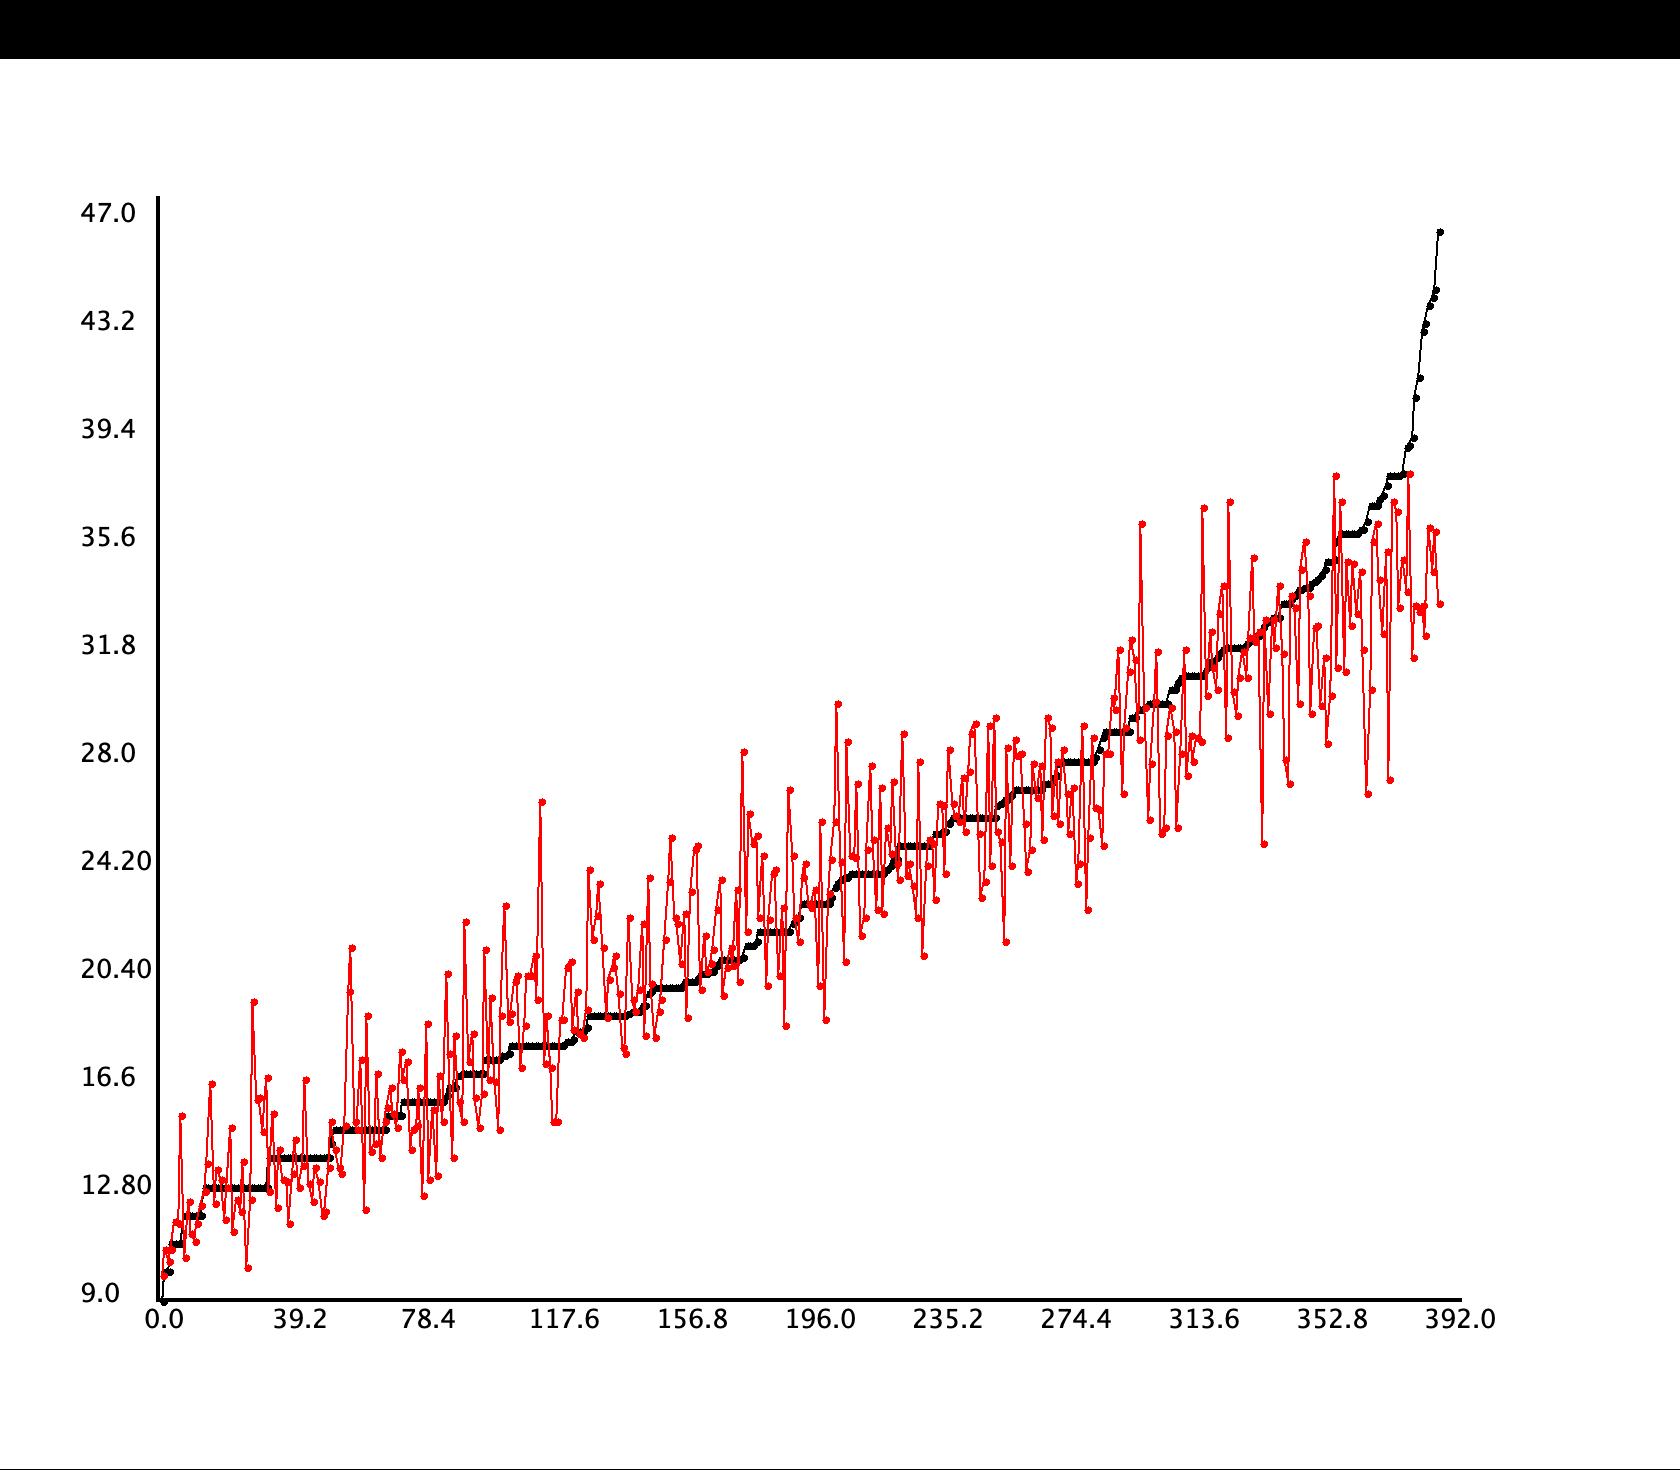
\includegraphics[width=\textwidth]{../Auto_MPG_Scalation_Plots/Scalation_Log1p_In_Sample.png}
     \end{subfigure}
     \hfill
     \begin{subfigure}[b]{0.4\textwidth}
         \centering
         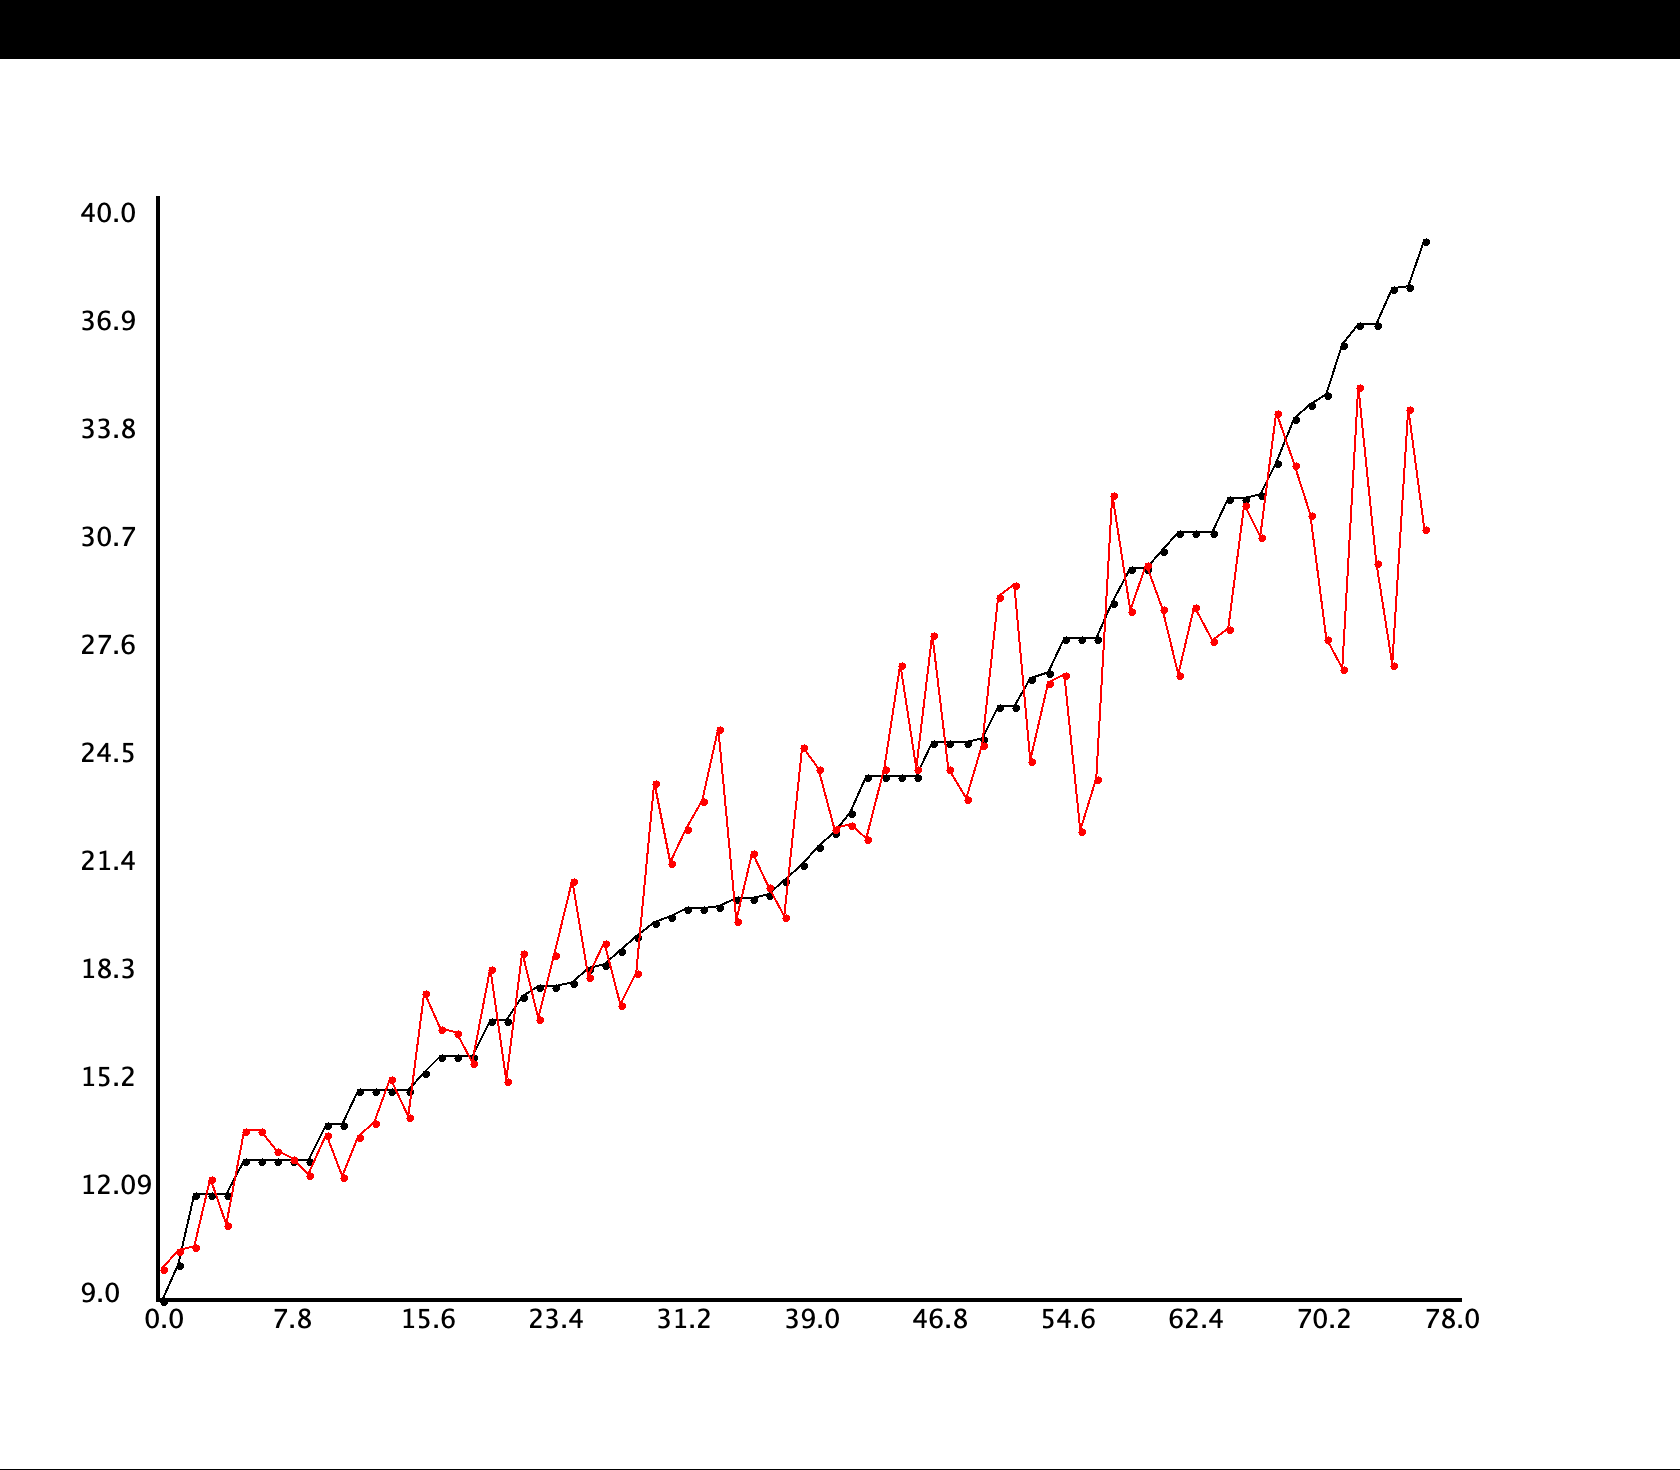
\includegraphics[width=\textwidth]{../Auto_MPG_Scalation_Plots/Scalation_Log1p_80_20.png}
     \end{subfigure}

     \vspace{10pt} % Add some vertical spacing between rows

     % Second Row
     \begin{subfigure}[b]{0.49\textwidth}
         \centering
         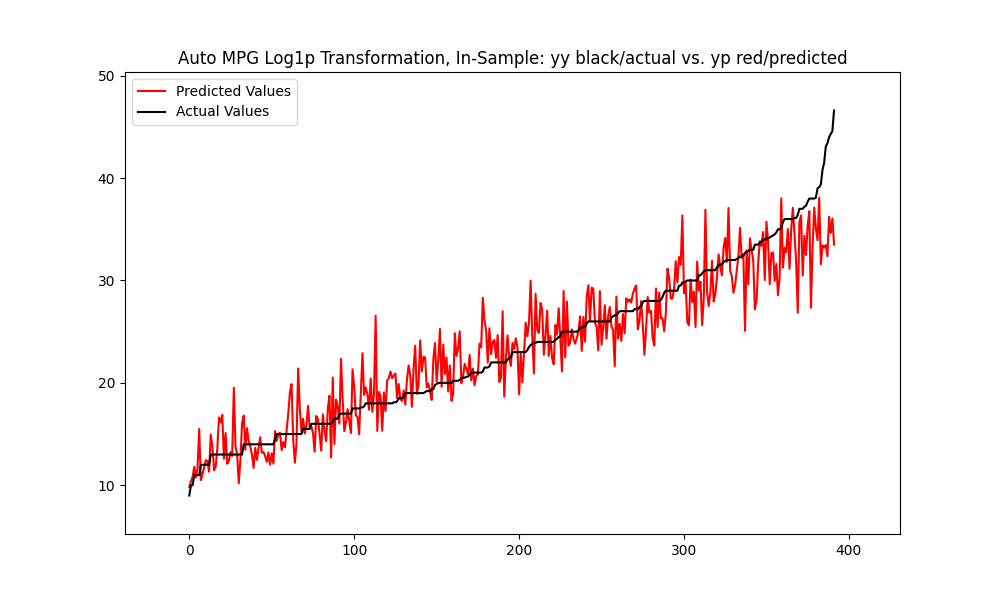
\includegraphics[width=\textwidth]{../Auto_MPG_Statsmodels_Plots/Statsmodels_Log1p_In_Sample.png}
     \end{subfigure}
     \hfill
     \begin{subfigure}[b]{0.49\textwidth}
         \centering
         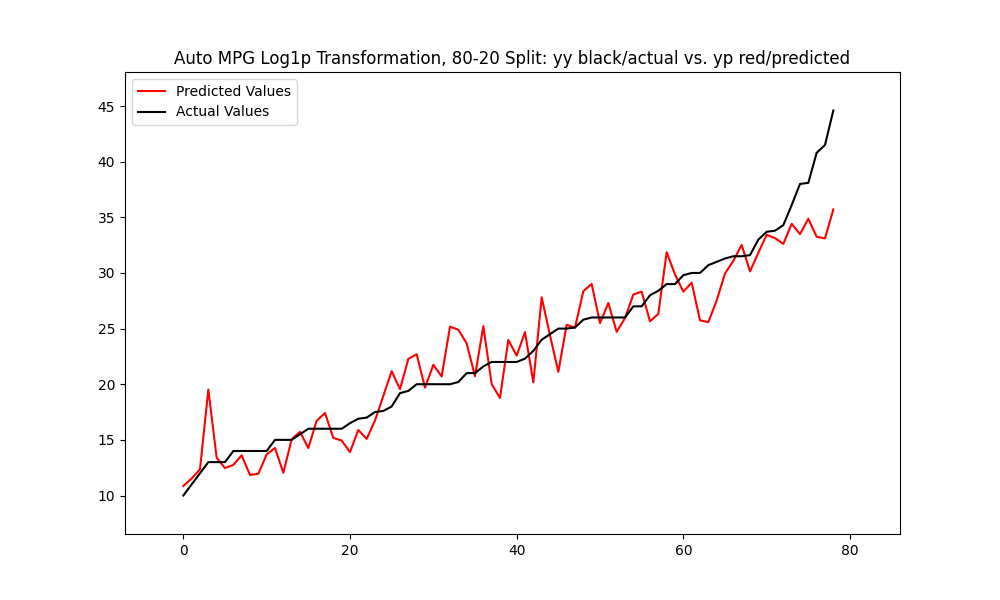
\includegraphics[width=\textwidth]{../Auto_MPG_Statsmodels_Plots/Statsmodels_Log1p_80_20.png}
     \end{subfigure}
     
     \caption{Auto MPG Log1p Transformation Plots\\ Top Left: Scalation In-Sample, Top Right: Scalation Out-of-Sample\\ Bottom Left: Statsmodels In-Sample, Bottom Right: Statsmodels Out-of-Sample\\ black: actual y-values, red: predicted y-values}
     \label{fig:Auto MPG Log1p Transformation Plots}
\end{figure}

\begin{table}[H]
\centering
\caption{Scalation - Auto MPG Log1p Transformation}
\label{tab:Scalation - Auto MPG Log1p Transformation}
\begin{tabular}{|c|c|c|} \hline 
Metric & In-Sample & 80-20 Split \\ \hline \hline 
rSq &0.859050 & 0.856892 \\ \hline 
rSqBar &0.856105 &      0.853903 \\ \hline 
sst &23819.0 &  4731.23 \\ \hline 
sse &3357.30 &  677.077 \\ \hline 
sde &2.92430 &  2.90754 \\ \hline 
mse0 &8.56453 & 8.68048 \\ \hline 
rmse &2.92652 & 2.94626 \\ \hline 
mae &2.12419 &  2.03303 \\ \hline 
smape &9.04308 &        8.33155 \\ \hline 
m &392.000 &    78.0000 \\ \hline 
dfr &8.00000 &  8.00000 \\ \hline 
df &383.000 &   383.000 \\ \hline 
fStat &291.783 &        286.663 \\ \hline 
aic &-959.161 & -176.990 \\ \hline 
bic &-923.420 & -155.779 \\ \hline 
\end{tabular}
\end{table}

\begin{table}[H]
\centering
\caption{Statsmodels - Auto MPG Log1p Transformation}
\label{tab:Statsmodels - Auto MPG Log1p Transformation}
\begin{tabular}{|c|c|c|}\hline
Metric & In-Sample & 80-20 Split \\ \hline \hline
rSq & 0.8800 & 0.8786 \\ \hline
rSqBar & 0.8775 & 0.8647 \\ \hline
sst & 41.1728 & 4910.2699 \\ \hline
sse & 4.9408 & 596.2565 \\ \hline
sde & 0.1136 & 2.9186 \\ \hline
mse0 & 0.0129 & 7.5476 \\ \hline
rmse & 0.1136 & 2.7473 \\ \hline
mae & 2.1242 & 2.0120 \\ \hline
smape & 9.0431 & 8.6767 \\ \hline
m & 392.0000 & 79.0000 \\ \hline
dfr & 8.0000 & 9.0000 \\ \hline
df & 383.0000 & 70.0000 \\ \hline
fStat & 351.0758 & 56.2735 \\ \hline
aic & -584.0540 & 177.6766 \\ \hline
bic & -548.3126 & 199.0016 \\ \hline
\end{tabular}
\end{table}

\begin{table}[H]
\centering
\caption{Scalation - Auto MPG Log1p Transformation CV}
\label{tab:Scalation - Auto MPG Log1p Transformation CV}
\begin{tabular}{|c|c|c|c|c|c|}\hline
Metric & num folds & min & max & mean & stdev \\ \hline \hline
rSq & 5 & 0.830 & 0.864 & 0.849 & 0.013 \\ \hline
rSqBar & 5 & 0.827 & 0.861 & 0.845 & 0.013 \\ \hline
sst & 5 & 3962.818 & 5671.580 & 4700.481 & 620.767 \\ \hline
sse & 5 & 539.065 & 872.917 & 713.304 & 121.664 \\ \hline
sde & 5 & 2.594 & 3.199 & 2.976 & 0.239 \\ \hline
mse0 & 5 & 6.911 & 11.191 & 9.145 & 1.560 \\ \hline
rmse & 5 & 2.629 & 3.345 & 3.015 & 0.262 \\ \hline
mae & 5 & 2.015 & 2.396 & 2.181 & 0.159 \\ \hline
smape & 5 & 8.332 & 10.571 & 9.273 & 0.827 \\ \hline
m & 5 & 78.000 & 78.000 & 78.000 & 0.000 \\ \hline
dfr & 5 & 8.000 & 8.000 & 8.000 & 0.000 \\ \hline
df & 5 & 383.000 & 383.000 & 383.000 & 0.000 \\ \hline
fStat & 5 & 234.489 & 304.067 & 270.208 & 26.456 \\ \hline
aic & 5 & -188.723 & -168.721 & -179.160 & 7.289 \\ \hline
bic & 5 & -167.513 & -147.511 & -157.950 & 7.289 \\ \hline
\end{tabular}
\end{table}

\begin{table}[H]
\centering
\caption{Statsmodels - Auto MPG Log1p Transformation CV}
\label{tab:Statsmodels - Auto MPG Log1p Transformation CV}
\begin{tabular}{|c|c|c|c|c|c|}\hline
Metric & num folds & min & max & mean & stdev \\ \hline \hline
rSq & 5 & 0.7837 & 0.8787 & 0.8462 & 0.0347 \\ \hline
rSqBar & 5 & 0.7587 & 0.8647 & 0.8285 & 0.0387 \\ \hline
sst & 5 & 3880.9704 & 5093.9237 & 4721.1782 & 441.3031 \\ \hline
sse & 5 & 596.2565 & 839.3534 & 711.7754 & 92.4042 \\ \hline
sde & 5 & 2.9186 & 3.4878 & 3.1961 & 0.2137 \\ \hline
mse0 & 5 & 7.5476 & 10.7609 & 9.0822 & 1.2049 \\ \hline
rmse & 5 & 2.7473 & 3.2804 & 3.0070 & 0.2005 \\ \hline
mae & 5 & 2.0120 & 2.4756 & 2.1900 & 0.1748 \\ \hline
smape & 5 & 8.5238 & 11.1215 & 9.3196 & 0.9679 \\ \hline
m & 5 & 78.0000 & 79.0000 & 78.4000 & 0.4899 \\ \hline
dfr & 5 & 9.0000 & 9.0000 & 9.0000 & 0.0000 \\ \hline
df & 5 & 69.0000 & 70.0000 & 69.4000 & 0.4899 \\ \hline
fStat & 5 & 27.7822 & 56.2735 & 44.7718 & 10.4953 \\ \hline
aic & 5 & 177.6766 & 203.3220 & 190.2479 & 10.0430 \\ \hline
bic & 5 & 199.0016 & 224.5324 & 211.5042 & 10.0226 \\ \hline
\end{tabular}
\end{table}

\subsubsection{Feature Selection}

Scalation Forward Selection: intercept, origin 2, modelyear, acceleration, origin 3, horsepower, displacement, cylinders, weight

Statsmodels Forward Selection: intercept, weight, model year, horsepower, origin 2, origin 3, displacement, acceleration, cylinders

\begin{figure}[H]
     \centering
     \captionsetup{justification=centering}
     % First Row
     \begin{subfigure}[b]{0.4\textwidth}
         \centering
         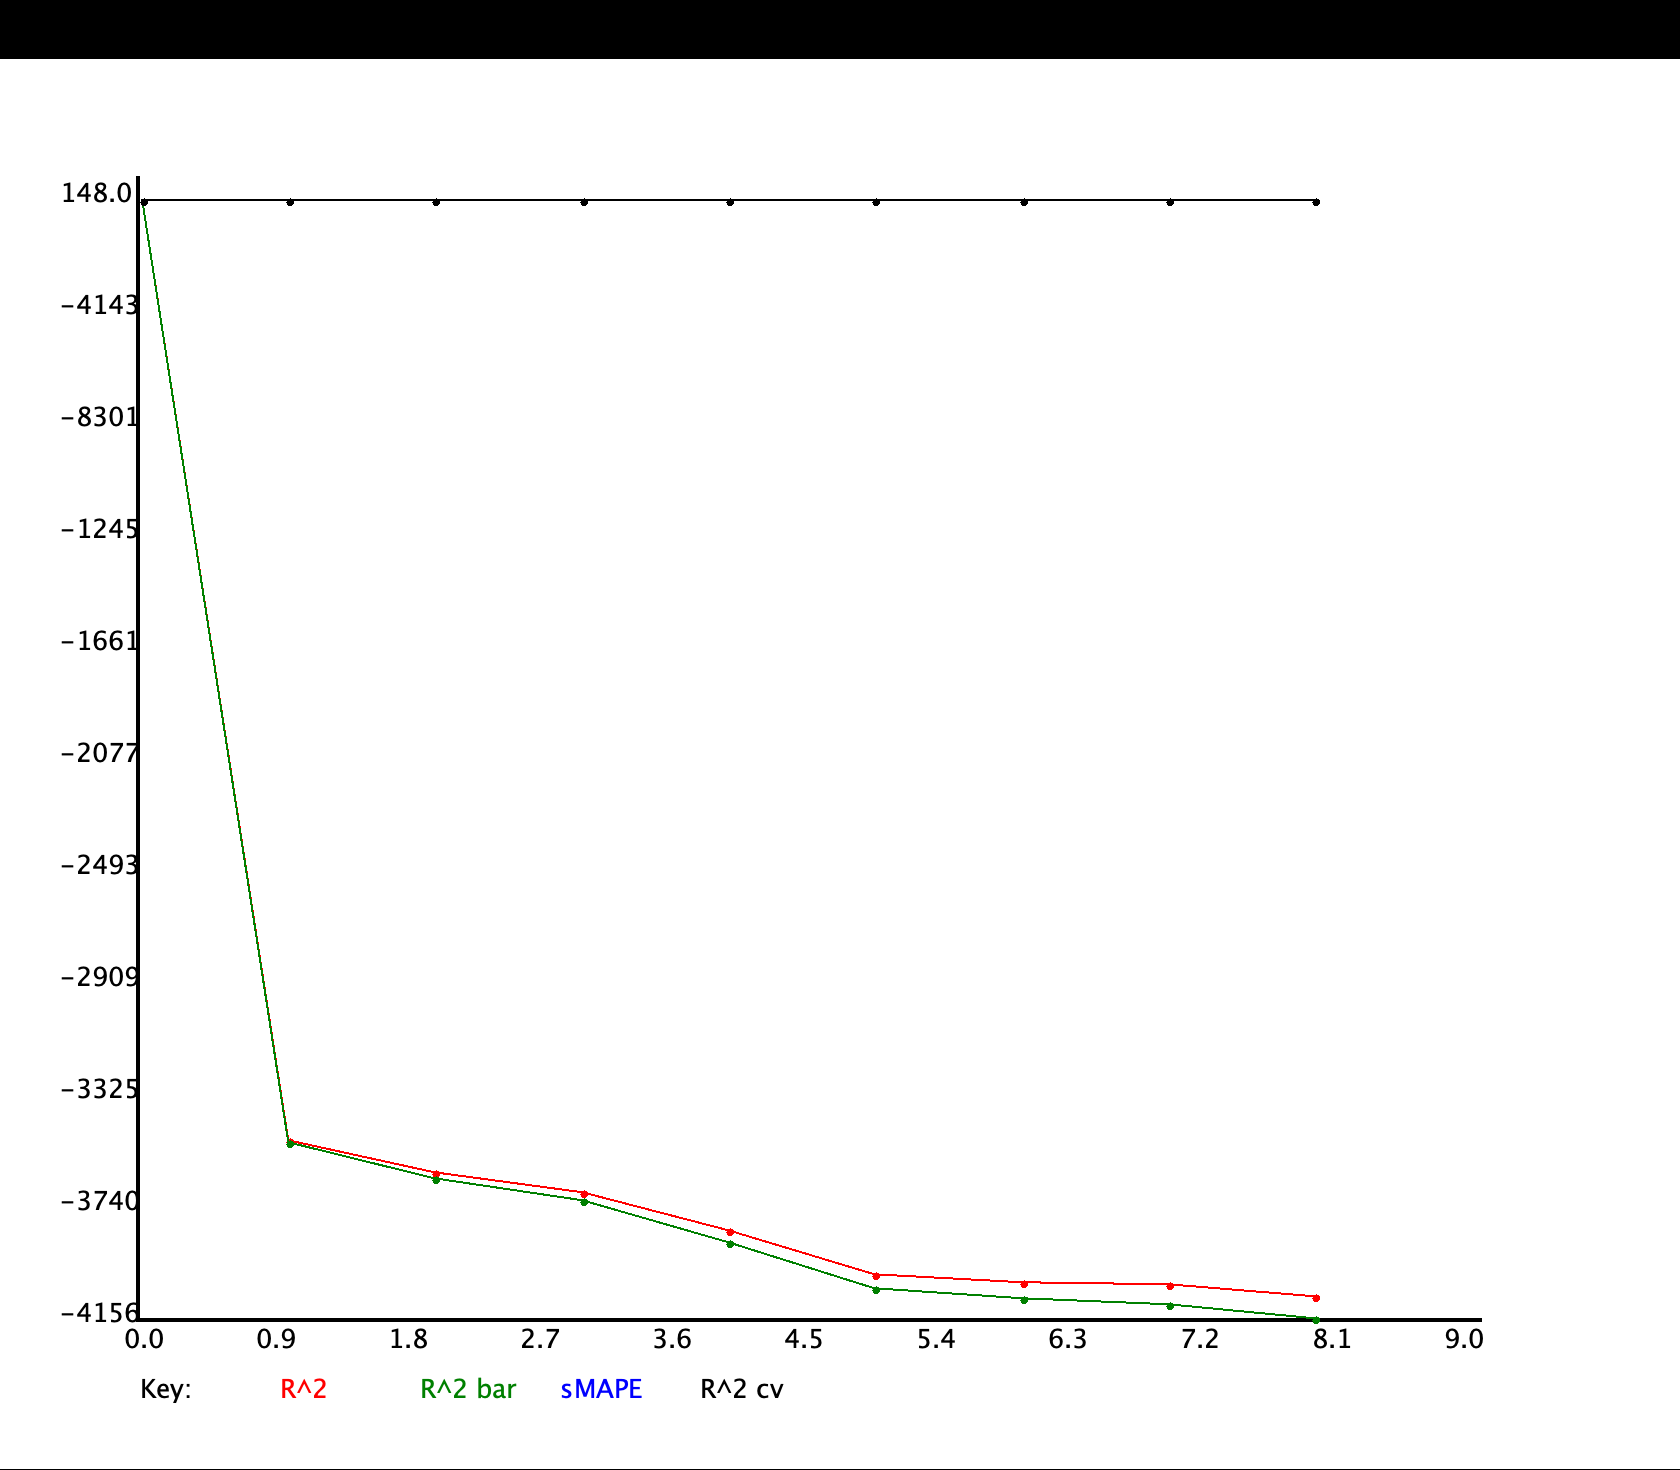
\includegraphics[width=\textwidth]{../Auto_MPG_Scalation_Plots/Scalation_Log1p_rSq_Forward.png}
     \end{subfigure}
     \hfill
     \begin{subfigure}[b]{0.4\textwidth}
         \centering
         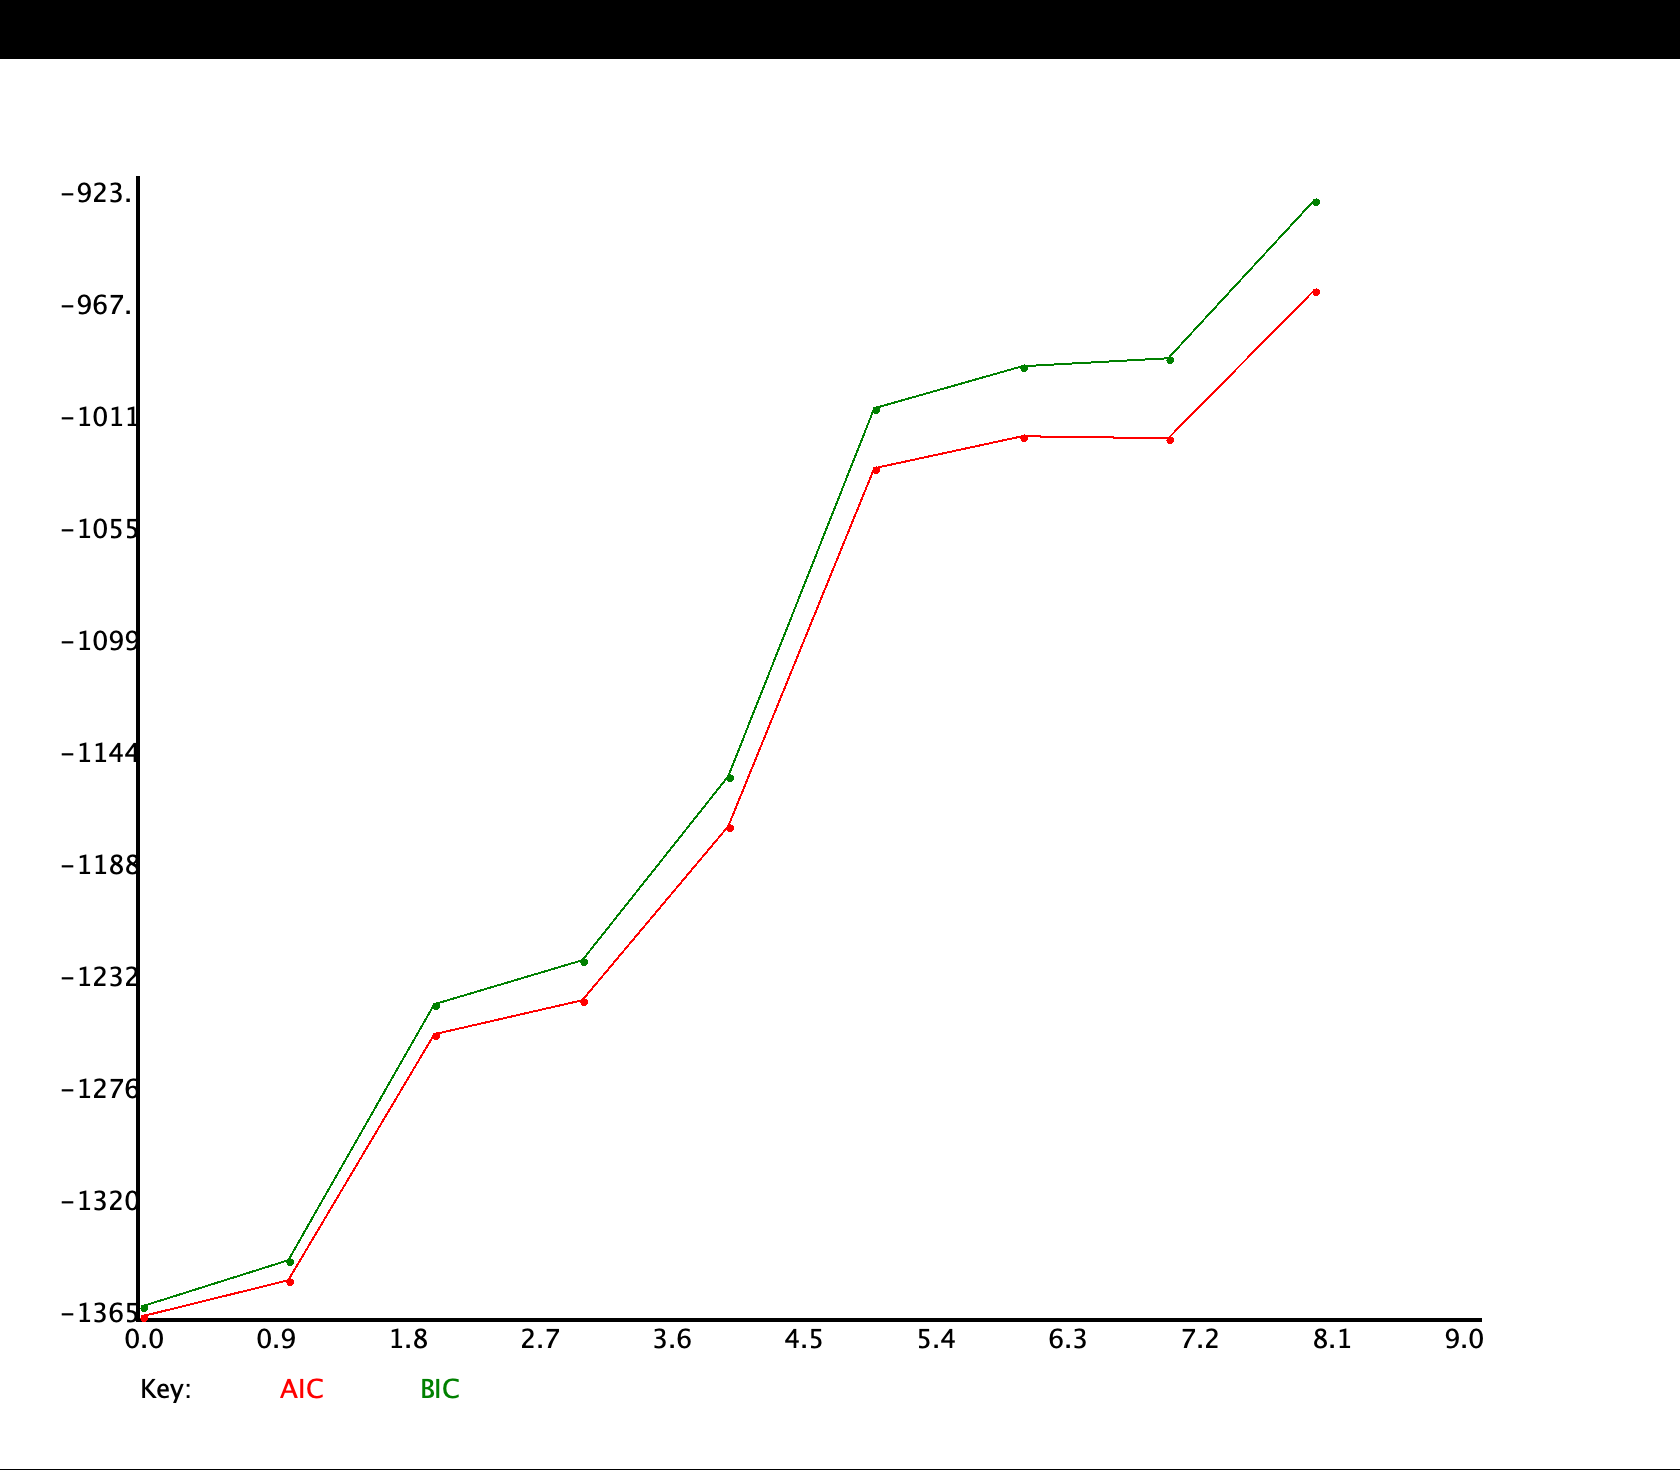
\includegraphics[width=\textwidth]{../Auto_MPG_Scalation_Plots/Scalation_Log1p_AIC_BIC_Forward.png}
     \end{subfigure}

     \vspace{10pt} % Add some vertical spacing between rows

     % Second Row
     \begin{subfigure}[b]{0.49\textwidth}
         \centering
         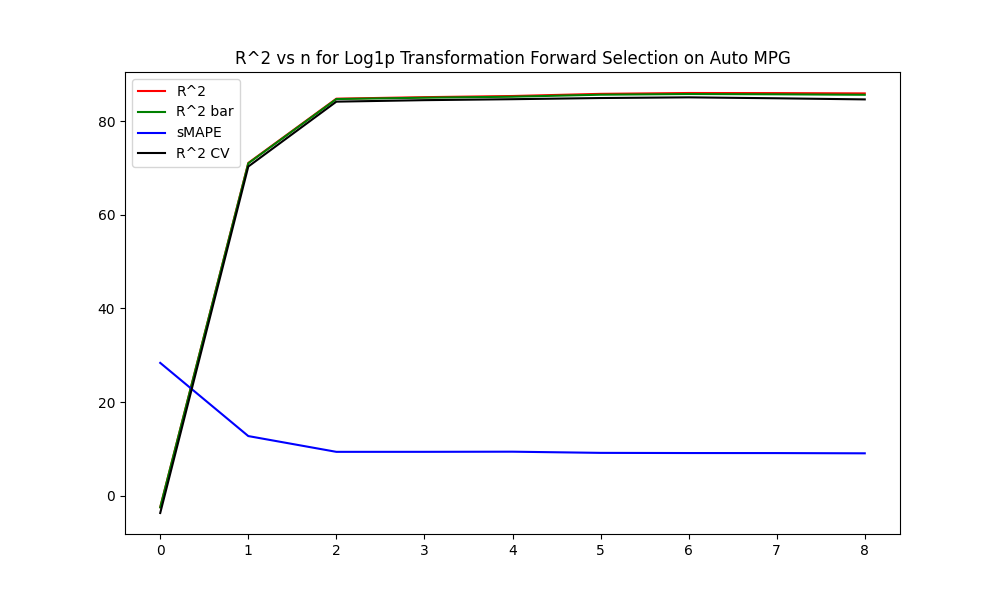
\includegraphics[width=\textwidth]{../Auto_MPG_Statsmodels_Plots/Statsmodels_Log1p_rSq_Forward.png}
     \end{subfigure}
     \hfill
     \begin{subfigure}[b]{0.49\textwidth}
         \centering
         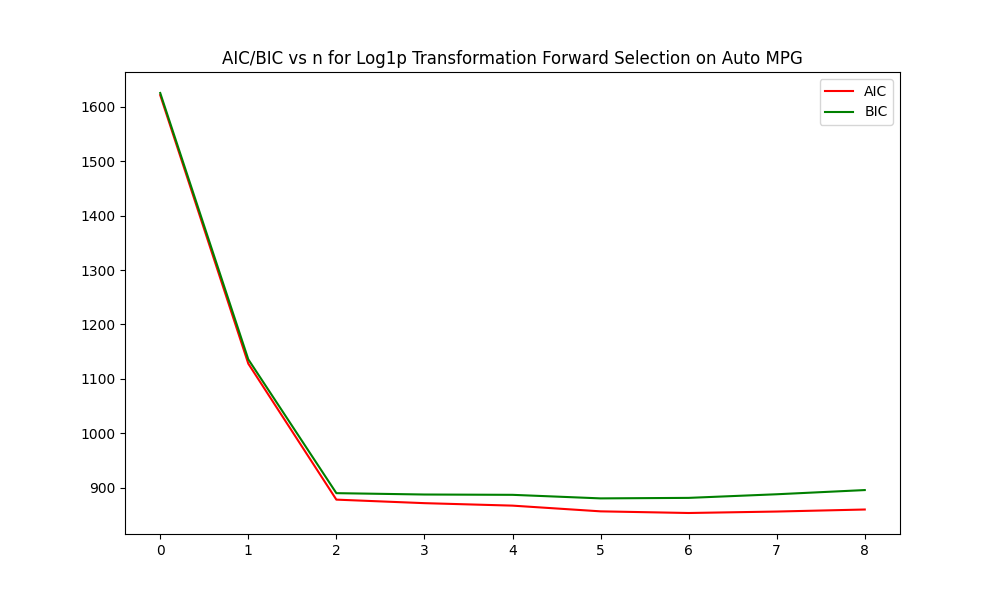
\includegraphics[width=\textwidth]{../Auto_MPG_Statsmodels_Plots/Statsmodels_Log1p_AIC_BIC_Forward.png}
     \end{subfigure}
     
     \caption{Auto MPG Log1p Transformation Forward Selection Quality of Fit Metrics\\ Top Left: Scalation $R^2$, Top Right: Scalation AIC/BIC\\ Bottom Left: Statsmodels $R^2$, Bottom Right: Statsmodels AIC/BIC}
     \label{fig:Auto MPG Log1p Transformation Forward Selection Quality of Fit Metrics}
\end{figure}

Scalation Backward Elimination Reversed: intercept, origin 2, origin 3, horsepower, displacement, cylinders, acceleration, weight, modelyear

Statsmodels Backward Elimination Reversed: intercept, weight, model year, origin 2, origin 3, horsepower, displacement, acceleration, cylinders

\begin{figure}[H]
     \centering
     \captionsetup{justification=centering}
     % First Row
     \begin{subfigure}[b]{0.4\textwidth}
         \centering
         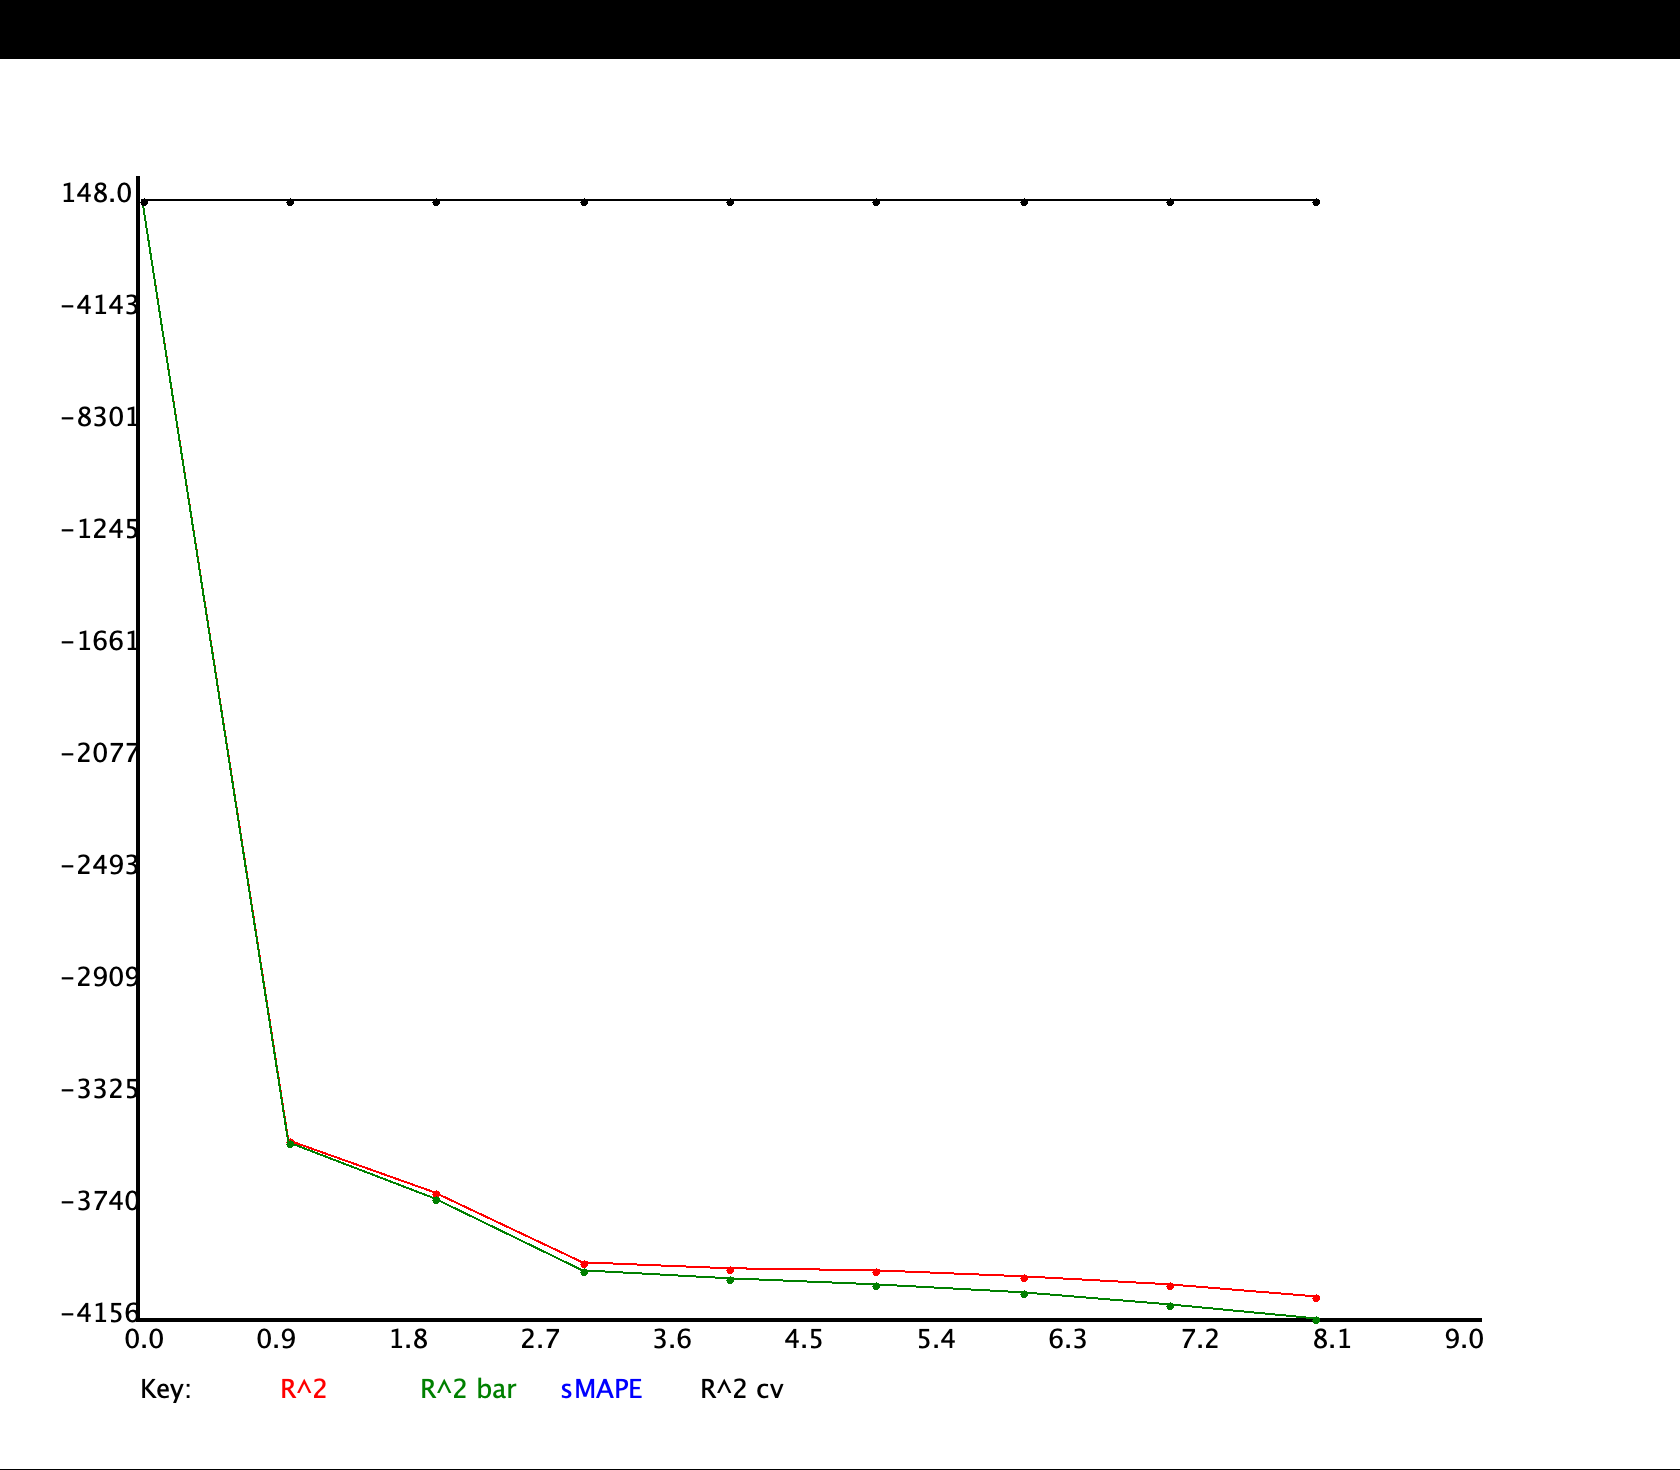
\includegraphics[width=\textwidth]{../Auto_MPG_Scalation_Plots/Scalation_Log1p_rSq_Backward.png}
     \end{subfigure}
     \hfill
     \begin{subfigure}[b]{0.4\textwidth}
         \centering
         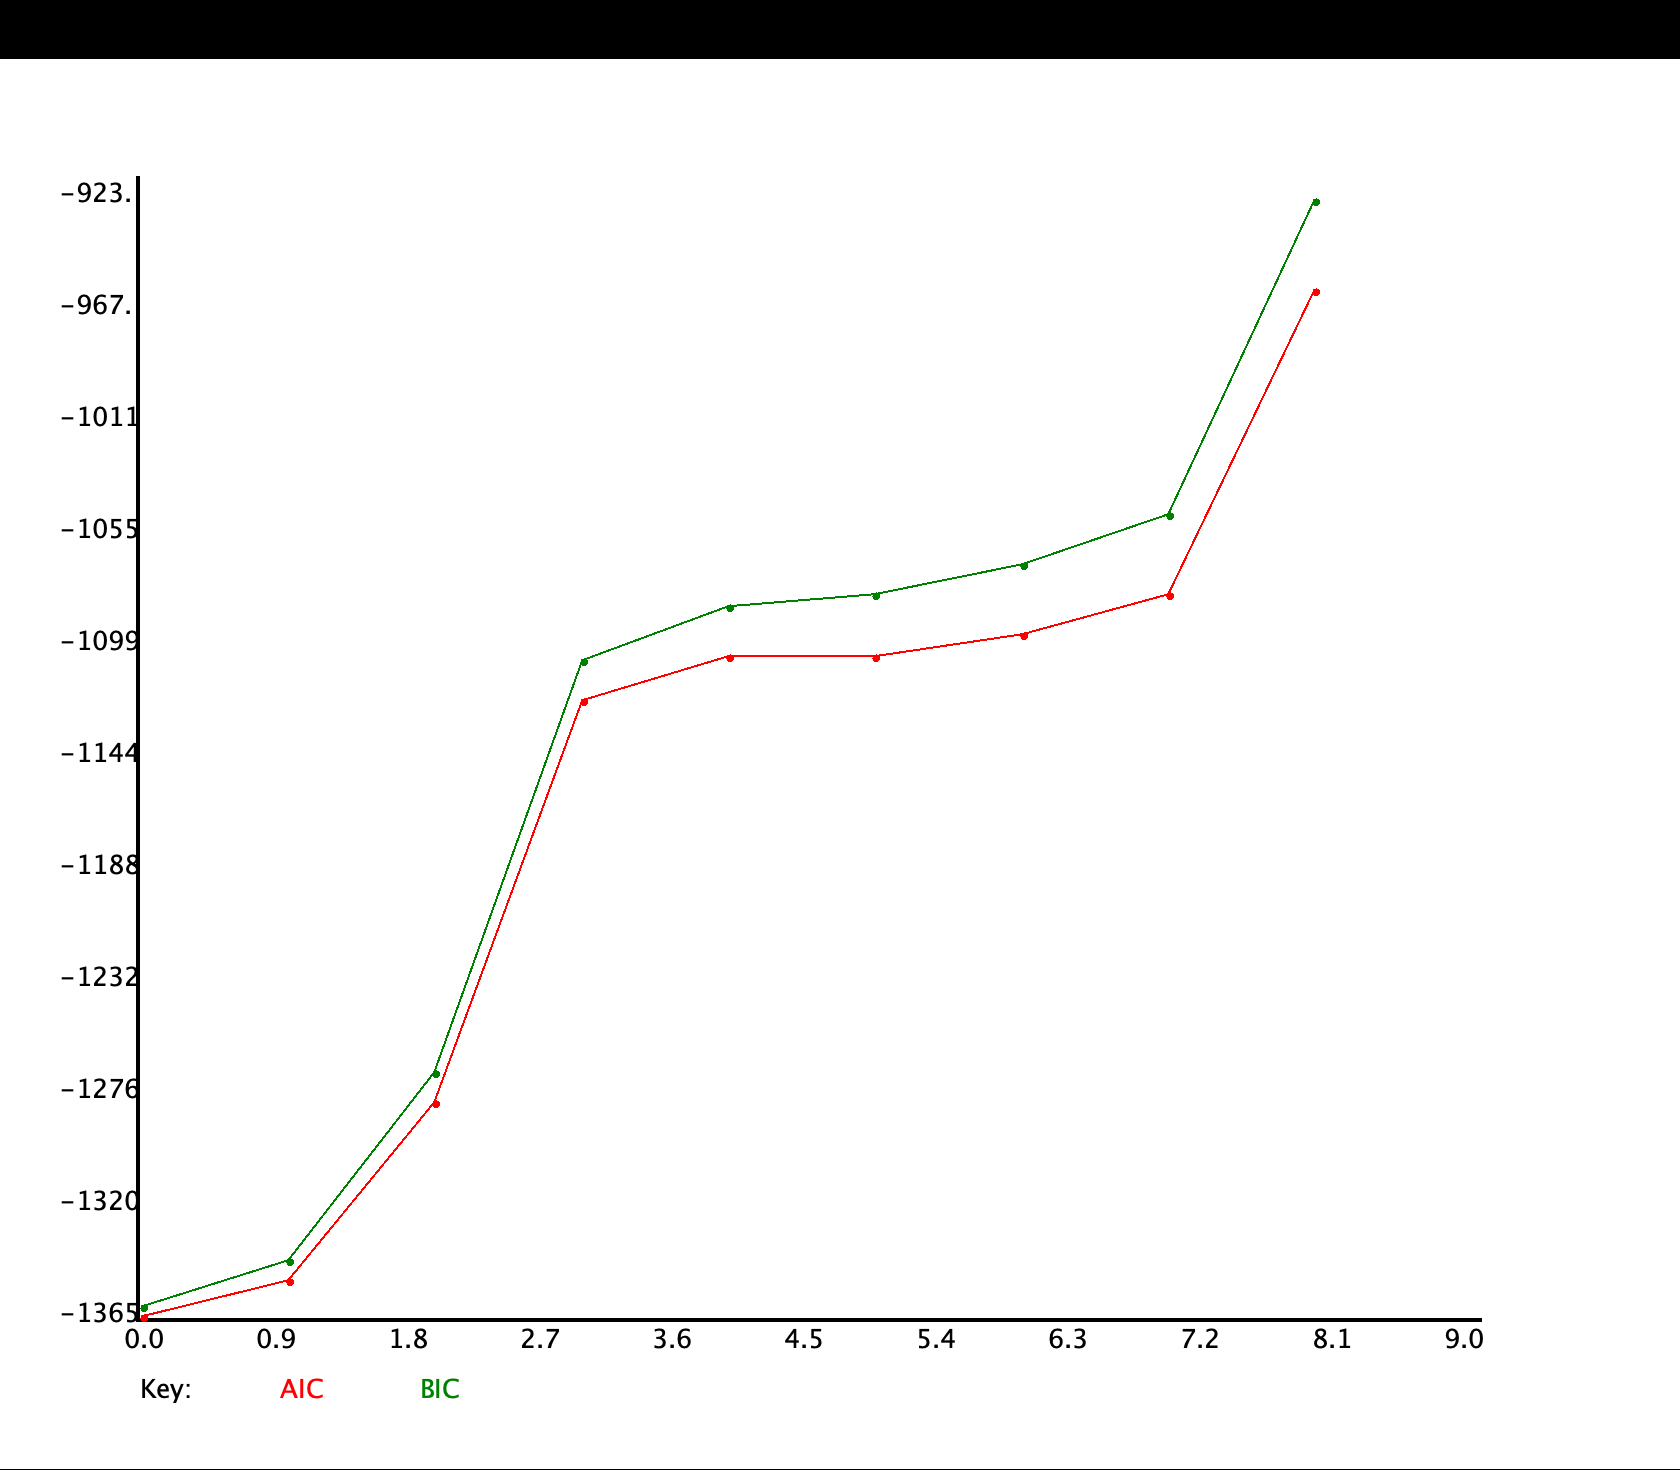
\includegraphics[width=\textwidth]{../Auto_MPG_Scalation_Plots/Scalation_Log1p_AIC_BIC_Backward.png}
     \end{subfigure}

     \vspace{10pt} % Add some vertical spacing between rows

     % Second Row
     \begin{subfigure}[b]{0.49\textwidth}
         \centering
         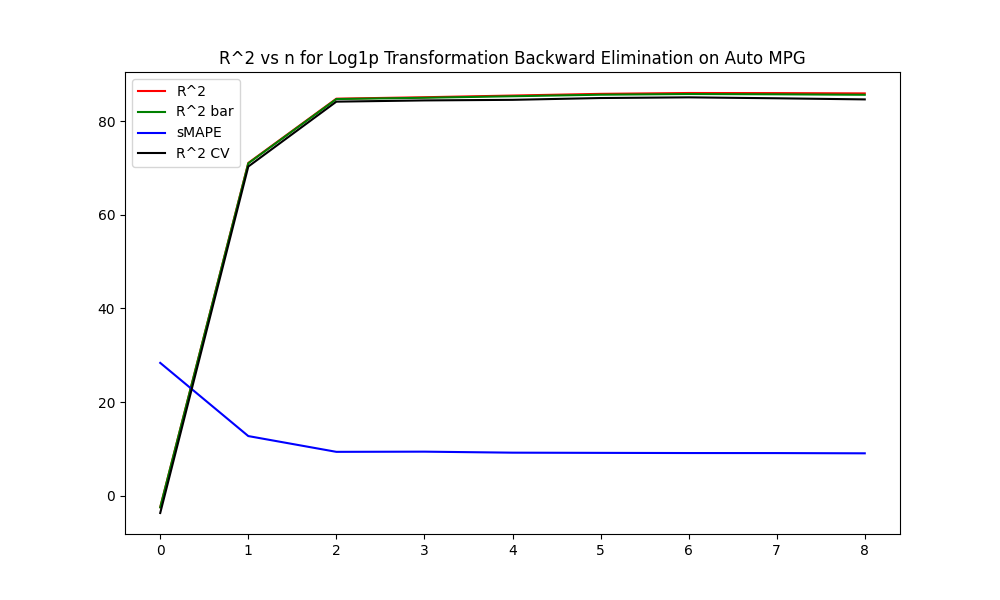
\includegraphics[width=\textwidth]{../Auto_MPG_Statsmodels_Plots/Statsmodels_Log1p_rSq_Backward.png}
     \end{subfigure}
     \hfill
     \begin{subfigure}[b]{0.49\textwidth}
         \centering
         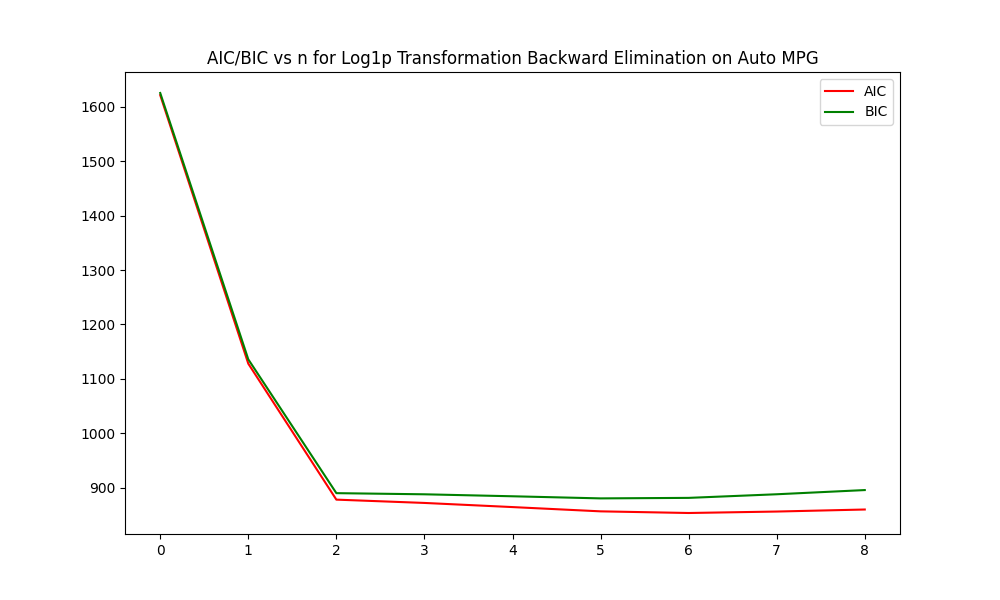
\includegraphics[width=\textwidth]{../Auto_MPG_Statsmodels_Plots/Statsmodels_Log1p_AIC_BIC_Backward.png}
     \end{subfigure}
     
     \caption{Auto MPG Log1p Transformation Reversed Backward Elimination Quality of Fit Metrics\\ Top Left: Scalation $R^2$, Top Right: Scalation AIC/BIC\\ Bottom Left: Statsmodels $R^2$, Bottom Right: Statsmodels AIC/BIC}
     \label{fig:Auto MPG Log1p Transformation Reversed Backward Elimination Quality of Fit Metrics}
\end{figure}

Scalation Stepwise Selection: intercept

Statsmodels Stepwise Selection: intercept, weight, model year, horsepower, origin 2, origin 3, displacement

\begin{figure}[H]
     \centering
     \captionsetup{justification=centering}
%     % First Row
%     \begin{subfigure}[b]{0.4\textwidth}
%         \centering
%         %\includegraphics[width=\textwidth]{../Auto_MPG_Scalation_Plots/Scalation_Log1p_rSq_Stepwise.png}
%     \end{subfigure}
%     \hfill
%     \begin{subfigure}[b]{0.4\textwidth}
%         \centering
%         %\includegraphics[width=\textwidth]{../Auto_MPG_Scalation_Plots/Scalation_Log1p_AIC_BIC_Stepwise.png}
%     \end{subfigure}
%
%     \vspace{10pt} % Add some vertical spacing between rows

     % Second Row
     \begin{subfigure}[b]{0.49\textwidth}
         \centering
         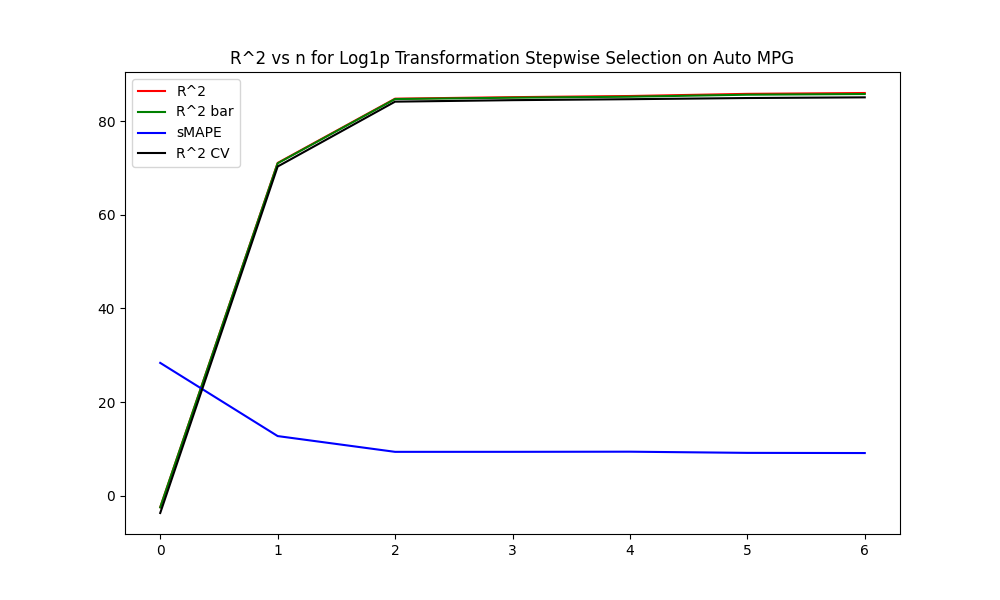
\includegraphics[width=\textwidth]{../Auto_MPG_Statsmodels_Plots/Statsmodels_Log1p_rSq_Stepwise.png}
     \end{subfigure}
     \hfill
     \begin{subfigure}[b]{0.49\textwidth}
         \centering
         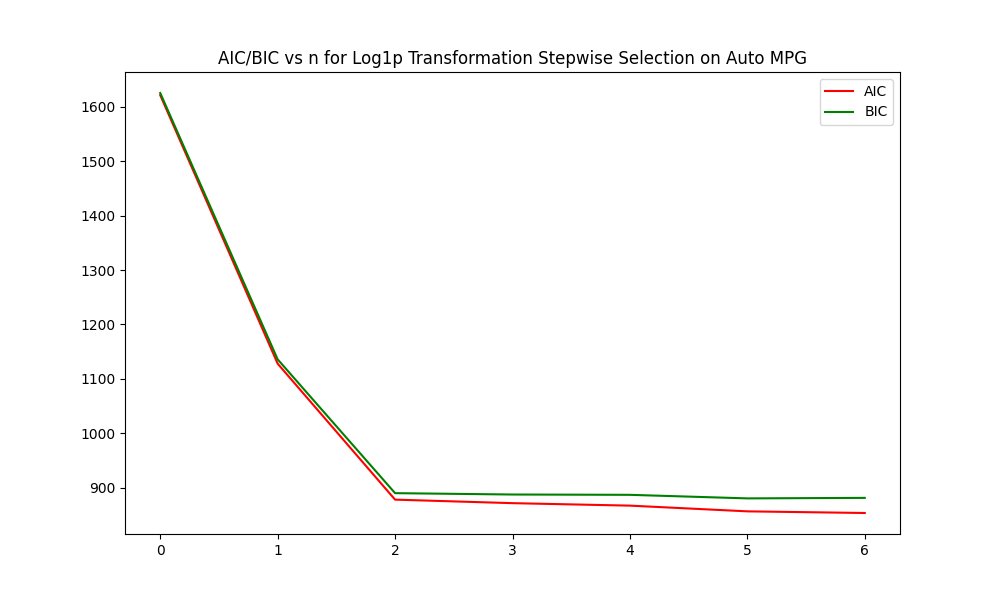
\includegraphics[width=\textwidth]{../Auto_MPG_Statsmodels_Plots/Statsmodels_Log1p_AIC_BIC_Stepwise.png}
     \end{subfigure}
     
     \caption{Auto MPG Log1p Transformation Stepwise Selection Quality of Fit Metrics\\ Left: Statsmodels $R^2$, Right: Statsmodels AIC/BIC}
     \label{fig:Auto MPG Log1p Transformation Stepwise Selection Quality of Fit Metrics}
\end{figure}

\subsection{Box-Cox Transformation}

\subsubsection{Quality of Fit}

Scalation Auto MPG Box-Cox Lambda Used: $-0.5$

\noindent Statsmodels Auto MPG Box-Cox lambda Used: $-0.5$

\begin{figure}[H]
     \centering
     \captionsetup{justification=centering}
     % First Row
     \begin{subfigure}[b]{0.4\textwidth}
         \centering
         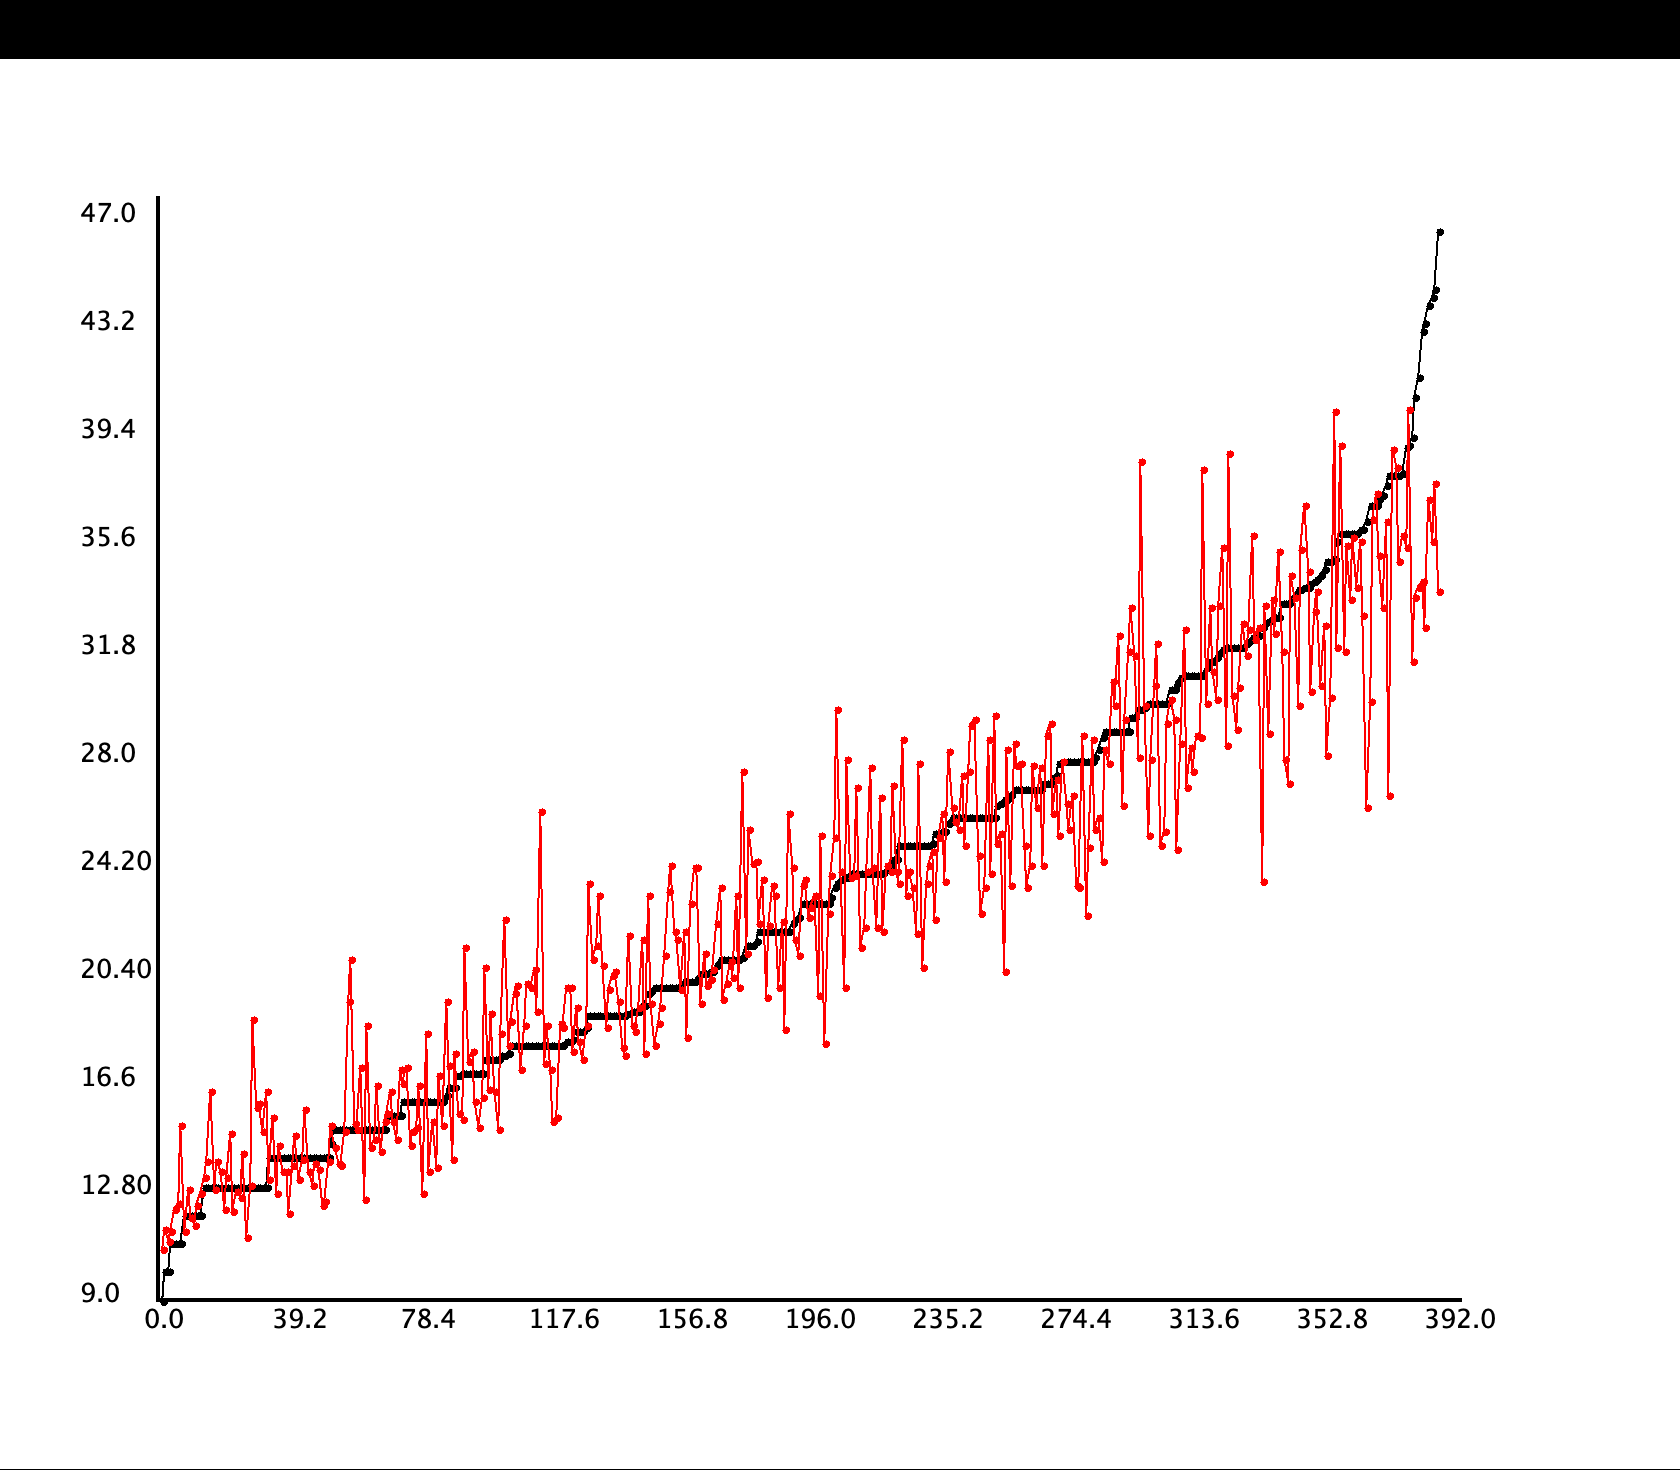
\includegraphics[width=\textwidth]{../Auto_MPG_Scalation_Plots/Scalation_BoxCox_In_Sample.png}
     \end{subfigure}
     \hfill
     \begin{subfigure}[b]{0.4\textwidth}
         \centering
         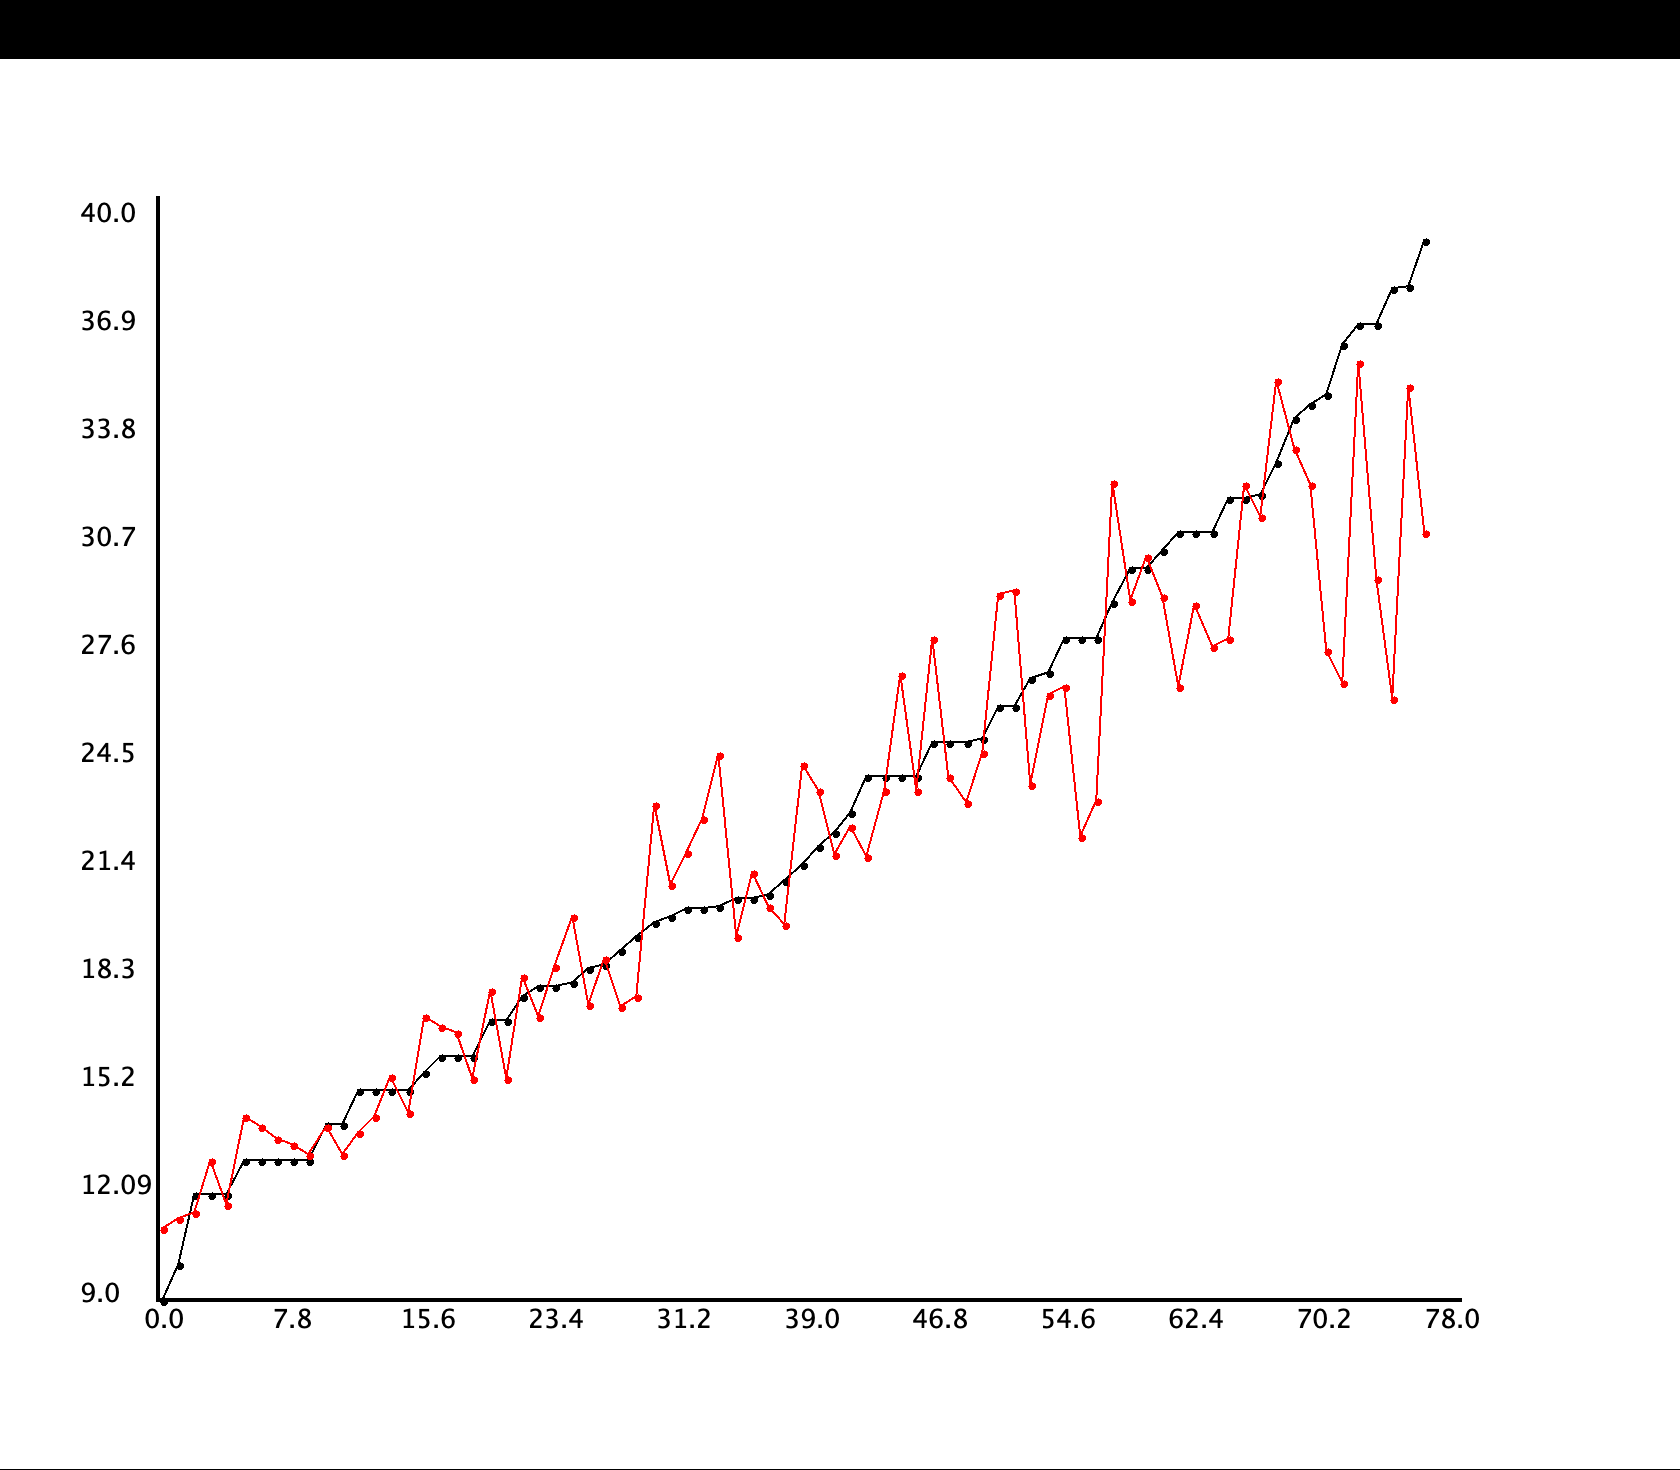
\includegraphics[width=\textwidth]{../Auto_MPG_Scalation_Plots/Scalation_BoxCox_80_20.png}
     \end{subfigure}

     \vspace{10pt} % Add some vertical spacing between rows

     % Second Row
     \begin{subfigure}[b]{0.49\textwidth}
         \centering
         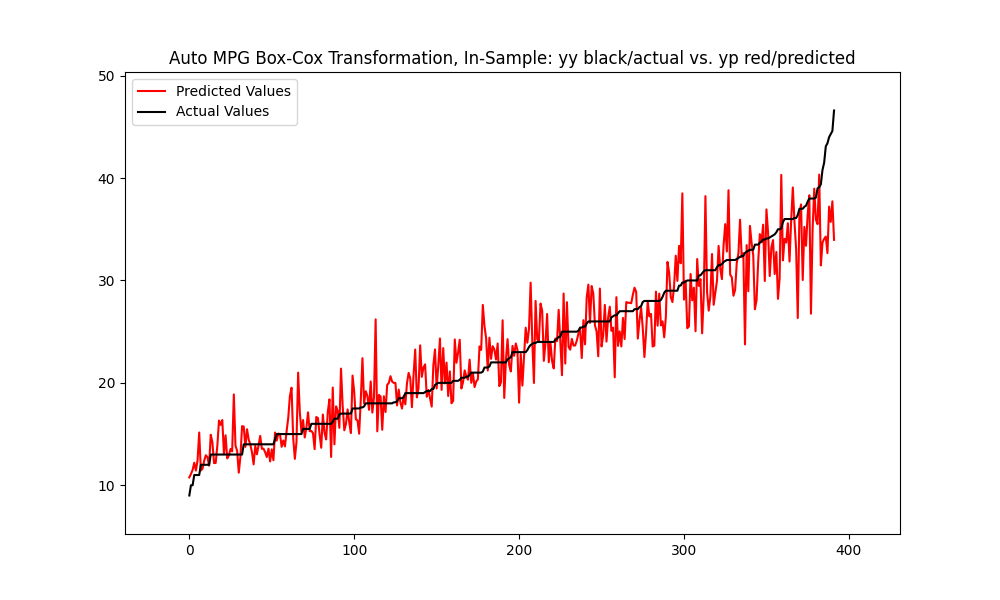
\includegraphics[width=\textwidth]{../Auto_MPG_Statsmodels_Plots/Statsmodels_BoxCox_In_Sample.png}
     \end{subfigure}
     \hfill
     \begin{subfigure}[b]{0.49\textwidth}
         \centering
         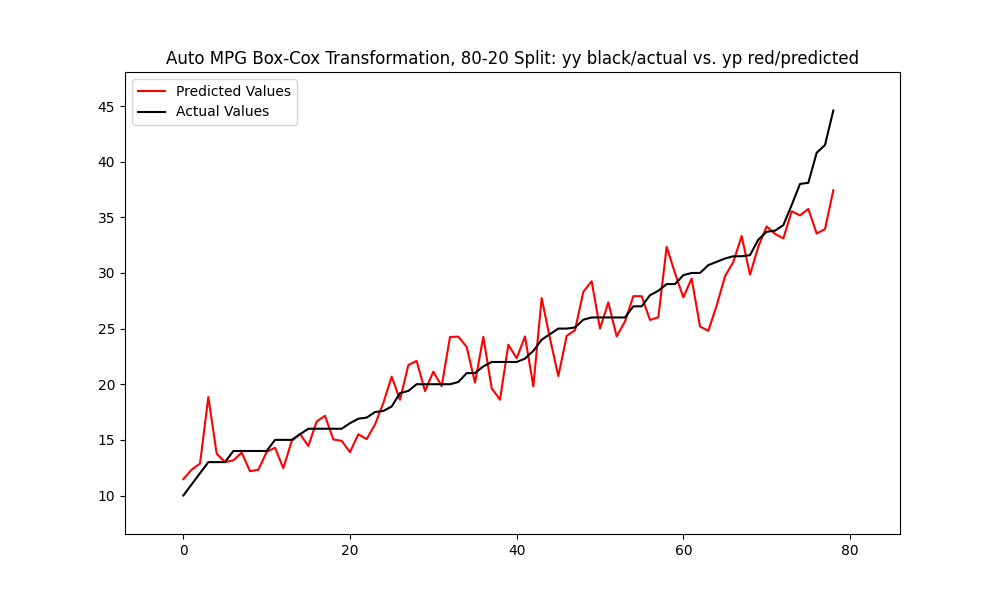
\includegraphics[width=\textwidth]{../Auto_MPG_Statsmodels_Plots/Statsmodels_BoxCox_80_20.png}
     \end{subfigure}
     
     \caption{Auto MPG Box-Cox Transformation Plots\\ Top Left: Scalation In-Sample, Top Right: Scalation Out-of-Sample\\ Bottom Left: Statsmodels In-Sample, Bottom Right: Statsmodels Out-of-Sample\\ black: actual y-values, red: predicted y-values}
     \label{fig:Auto MPG Box-Cox Transformation Plots}
\end{figure}

\begin{table}[H]
\centering
\caption{Scalation - Auto MPG Box-Cox Transformation}
\label{tab:Scalation - Auto MPG Box-Cox Transformation}
\begin{tabular}{|c|c|c|} \hline 
Metric & In-Sample & 80-20 Split \\ \hline \hline 
rSq &0.864986 & 0.852052 \\ \hline 
rSqBar &0.862166 &      0.848962 \\ \hline 
sst &23819.0 &  4731.23 \\ \hline 
sse &3215.90 &  699.976 \\ \hline 
sde &2.85675 &  2.93686 \\ \hline 
mse0 &8.20383 & 8.97405 \\ \hline 
rmse &2.86423 & 2.99567 \\ \hline 
mae &2.05497 &  2.02595 \\ \hline 
smape &8.67519 &        8.35081 \\ \hline 
m &392.000 &    78.0000 \\ \hline 
dfr &8.00000 &  8.00000 \\ \hline 
df &383.000 &   383.000 \\ \hline 
fStat &306.717 &        275.719 \\ \hline 
aic &-950.732 & -178.311 \\ \hline 
bic &-914.990 & -157.101 \\ \hline 
\end{tabular}
\end{table}

\begin{table}[H]
\centering
\caption{Statsmodels - Auto MPG Box-Cox Transformation}
\label{tab:Statsmodels - Auto MPG Box-Cox Transformation}
\begin{tabular}{|c|c|c|}\hline
Metric & In-Sample & 80-20 Split \\ \hline \hline
rSq & 0.8914 & 0.8944 \\ \hline
rSqBar & 0.8891 & 0.8823 \\ \hline
sst & 2.1480 & 4910.2699 \\ \hline
sse & 0.2334 & 518.6048 \\ \hline
sde & 0.0247 & 2.7219 \\ \hline
mse0 & 0.0006 & 6.5646 \\ \hline
rmse & 0.0247 & 2.5622 \\ \hline
mae & 2.0550 & 1.9170 \\ \hline
smape & 8.6752 & 8.3751 \\ \hline
m & 392.0000 & 79.0000 \\ \hline
dfr & 8.0000 & 9.0000 \\ \hline
df & 383.0000 & 70.0000 \\ \hline
fStat & 392.8140 & 65.8640 \\ \hline
aic & -1780.7268 & 166.6538 \\ \hline
bic & -1744.9854 & 187.9789 \\ \hline
\end{tabular}
\end{table}

\begin{table}[H]
\centering
\caption{Scalation - Auto MPG Box-Cox CV}
\label{tab:Scalation - Auto MPG Box-Cox CV}
\begin{tabular}{|c|c|c|c|c|c|}\hline
Metric & num folds & min & max & mean & stdev \\ \hline \hline
rSq & 5 & 0.838 & 0.888 & 0.856 & 0.019 \\ \hline
rSqBar & 5 & 0.835 & 0.885 & 0.853 & 0.019 \\ \hline
sst & 5 & 3962.818 & 5671.580 & 4700.481 & 620.767 \\ \hline
sse & 5 & 444.522 & 827.663 & 679.185 & 141.435 \\ \hline
sde & 5 & 2.389 & 3.148 & 2.908 & 0.300 \\ \hline
mse0 & 5 & 5.699 & 10.611 & 8.708 & 1.813 \\ \hline
rmse & 5 & 2.387 & 3.257 & 2.936 & 0.326 \\ \hline
mae & 5 & 1.823 & 2.301 & 2.111 & 0.190 \\ \hline
smape & 5 & 8.242 & 10.111 & 8.898 & 0.746 \\ \hline
m & 5 & 78.000 & 78.000 & 78.000 & 0.000 \\ \hline
dfr & 5 & 8.000 & 8.000 & 8.000 & 0.000 \\ \hline
df & 5 & 383.000 & 383.000 & 383.000 & 0.000 \\ \hline
fStat & 5 & 247.552 & 378.920 & 290.795 & 50.854 \\ \hline
aic & 5 & -185.809 & -163.310 & -177.090 & 8.306 \\ \hline
bic & 5 & -164.599 & -142.100 & -155.880 & 8.306 \\ \hline
\end{tabular}
\end{table}

\begin{table}[H]
\centering
\caption{Statsmodels - Auto MPG Box-Cox Transformation CV}
\label{tab:Statsmodels - Auto MPG Box-Cox Transformation CV}
\begin{tabular}{|c|c|c|c|c|c|}\hline
Metric & num folds & min & max & mean & stdev \\ \hline \hline
rSq & 5 & 0.7917 & 0.8944 & 0.8531 & 0.0356 \\ \hline
rSqBar & 5 & 0.7676 & 0.8823 & 0.8362 & 0.0397 \\ \hline
sst & 5 & 3880.9704 & 5093.9237 & 4721.1782 & 441.3031 \\ \hline
sse & 5 & 518.6048 & 808.3934 & 679.6400 & 105.7450 \\ \hline
sde & 5 & 2.7219 & 3.4228 & 3.1201 & 0.2536 \\ \hline
mse0 & 5 & 6.5646 & 10.3640 & 8.6735 & 1.3761 \\ \hline
rmse & 5 & 2.5622 & 3.2193 & 2.9355 & 0.2380 \\ \hline
mae & 5 & 1.9170 & 2.3027 & 2.1170 & 0.1323 \\ \hline
smape & 5 & 8.3751 & 10.1422 & 8.9379 & 0.6391 \\ \hline
m & 5 & 78.0000 & 79.0000 & 78.4000 & 0.4899 \\ \hline
dfr & 5 & 9.0000 & 9.0000 & 9.0000 & 0.0000 \\ \hline
df & 5 & 69.0000 & 70.0000 & 69.4000 & 0.4899 \\ \hline
fStat & 5 & 29.1398 & 65.8640 & 47.7890 & 12.6584 \\ \hline
aic & 5 & 166.6538 & 200.3905 & 186.2788 & 12.4501 \\ \hline
bic & 5 & 187.9789 & 221.6009 & 207.5350 & 12.4231 \\ \hline
\end{tabular}
\end{table}

\subsubsection{Feature Selection}

Scalation Forward Selection: intercept, origin 2, modelyear, acceleration, origin 3, horsepower, displacement, cylinders, weight

Statsmodels Forward Selection: intercept, weight, model year, horsepower, origin 2, origin 3, displacement, cylinders, acceleration

\begin{figure}[H]
     \centering
     \captionsetup{justification=centering}
     % First Row
     \begin{subfigure}[b]{0.4\textwidth}
         \centering
         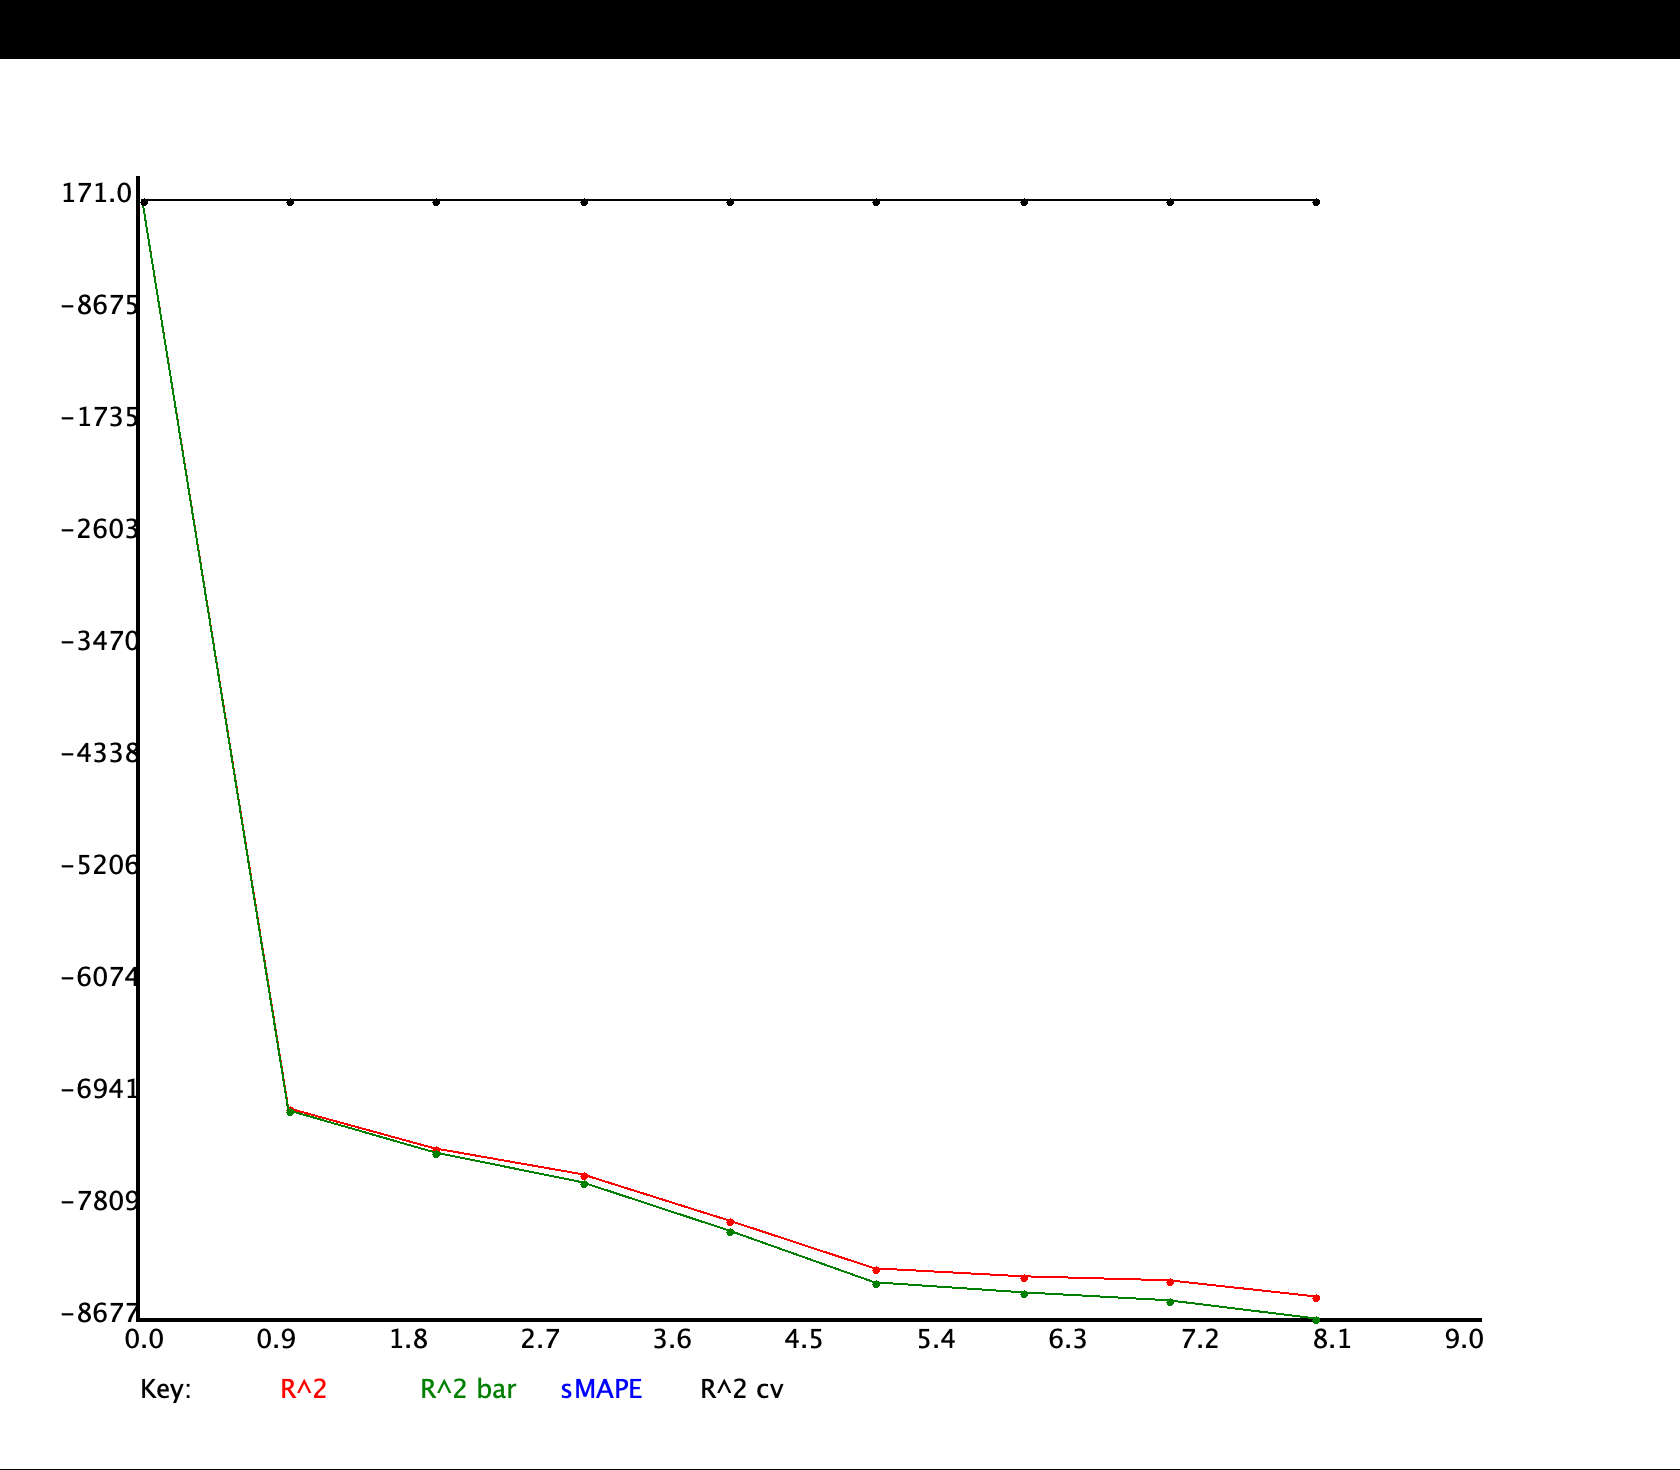
\includegraphics[width=\textwidth]{../Auto_MPG_Scalation_Plots/Scalation_BoxCox_rSq_Forward.png}
     \end{subfigure}
     \hfill
     \begin{subfigure}[b]{0.4\textwidth}
         \centering
         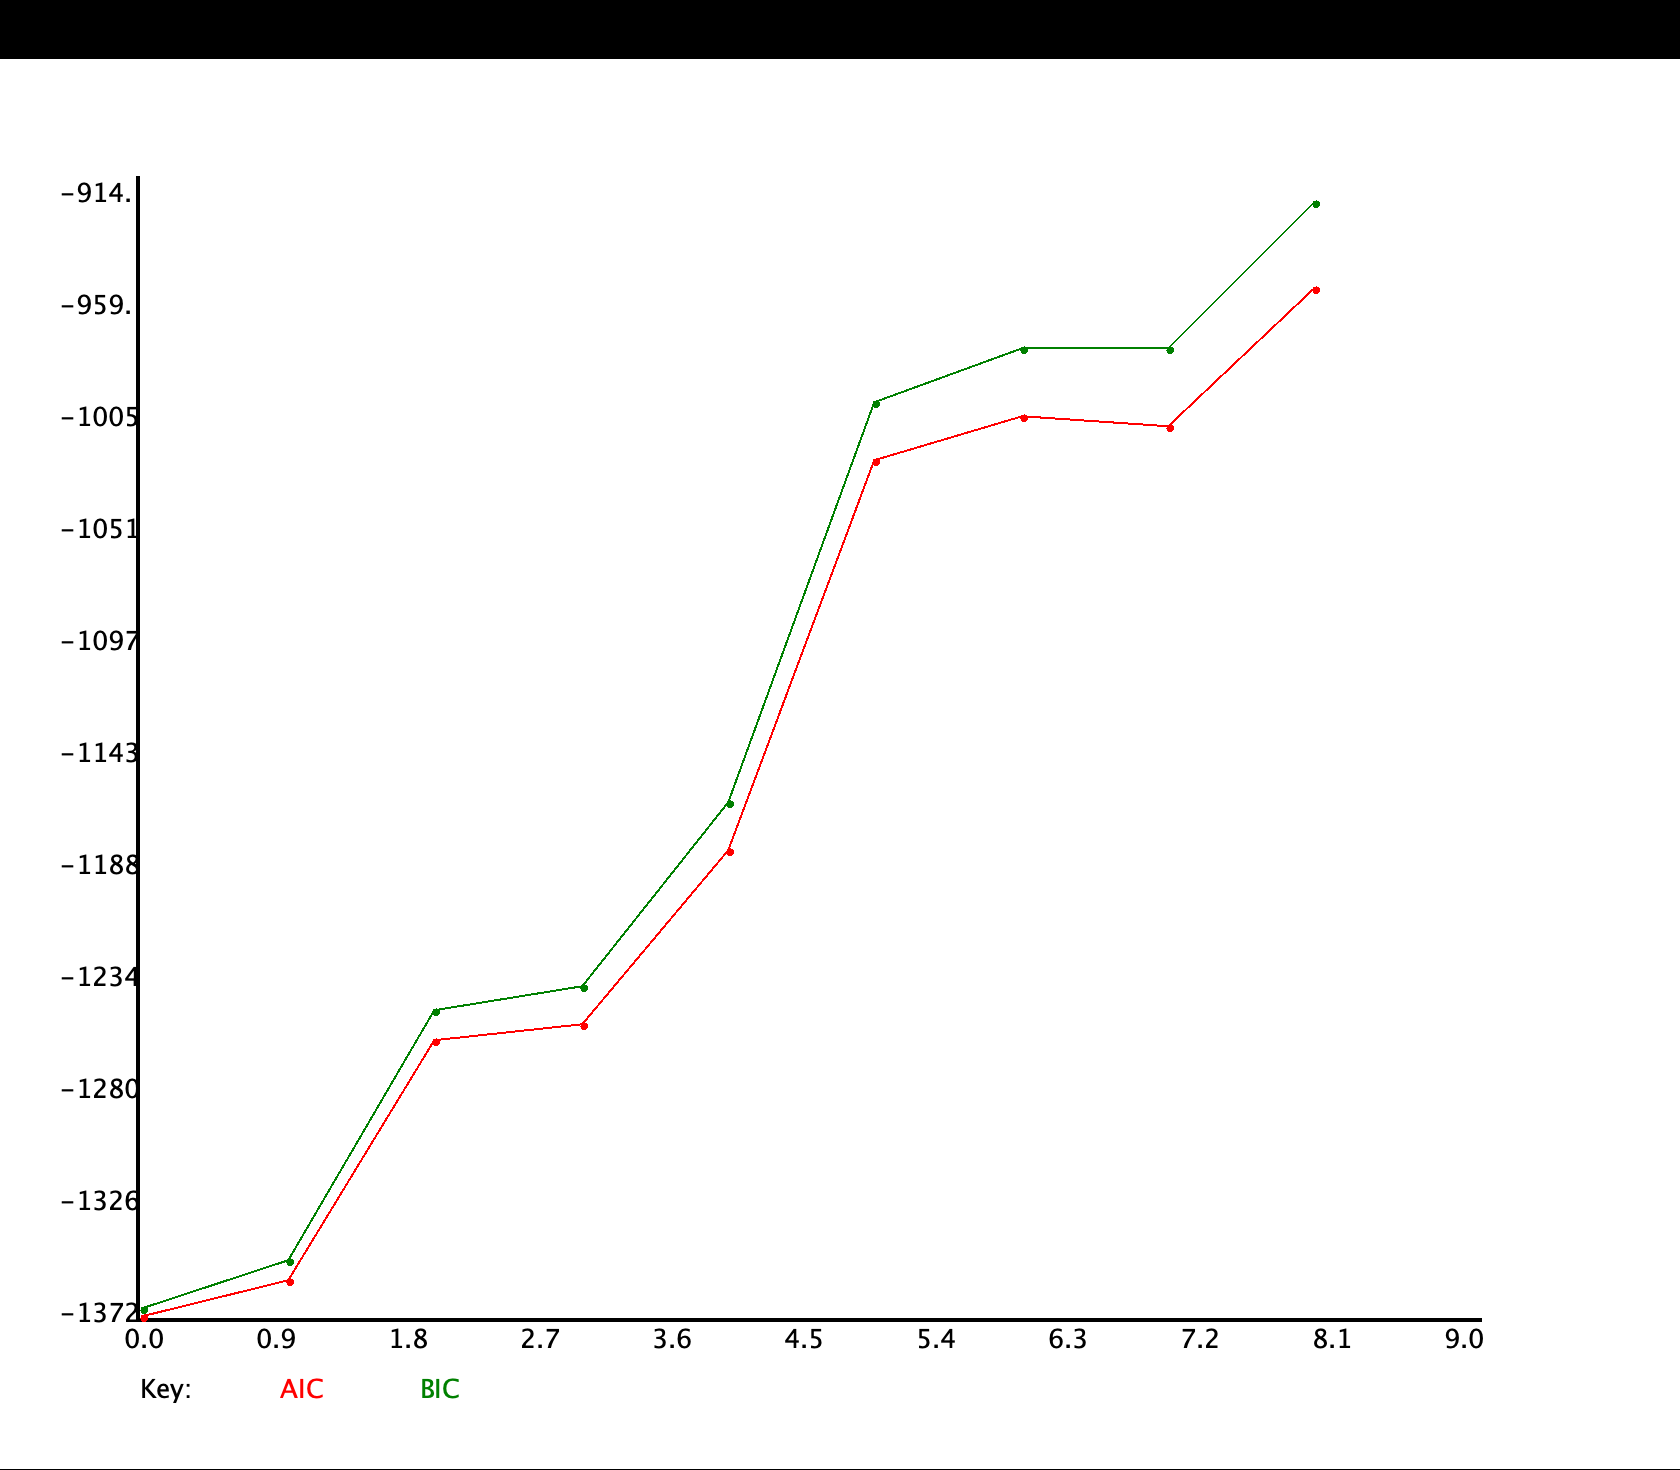
\includegraphics[width=\textwidth]{../Auto_MPG_Scalation_Plots/Scalation_BoxCox_AIC_BIC_Forward.png}
     \end{subfigure}

     \vspace{10pt} % Add some vertical spacing between rows

     % Second Row
     \begin{subfigure}[b]{0.49\textwidth}
         \centering
         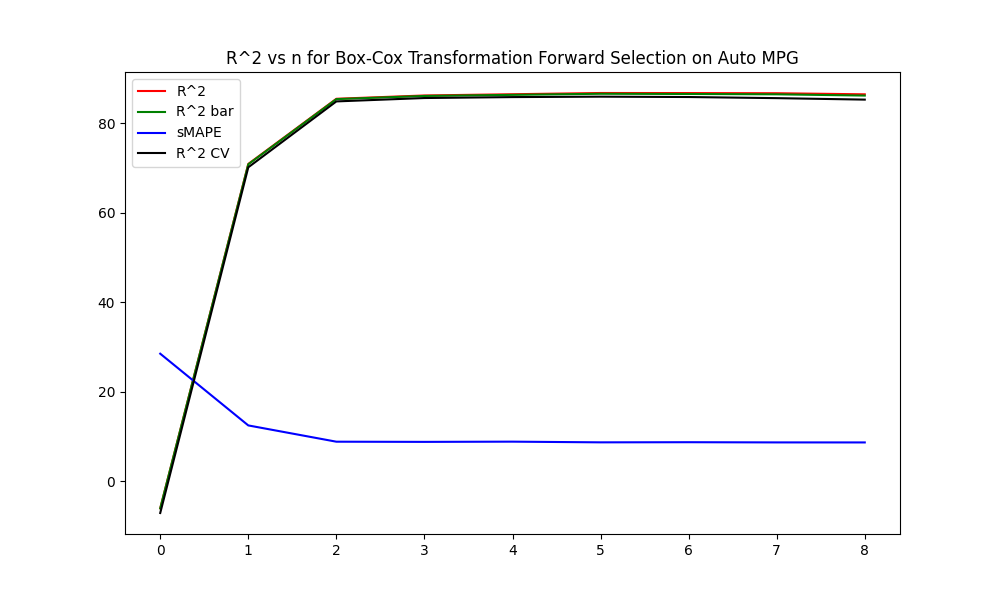
\includegraphics[width=\textwidth]{../Auto_MPG_Statsmodels_Plots/Statsmodels_BoxCox_rSq_Forward.png}
     \end{subfigure}
     \hfill
     \begin{subfigure}[b]{0.49\textwidth}
         \centering
         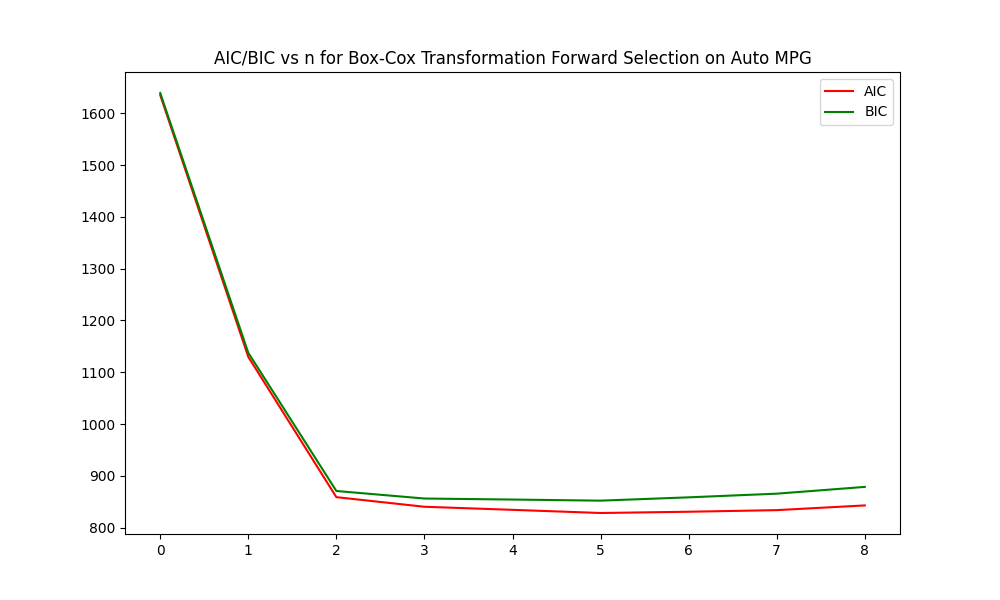
\includegraphics[width=\textwidth]{../Auto_MPG_Statsmodels_Plots/Statsmodels_BoxCox_AIC_BIC_Forward.png}
     \end{subfigure}
     
     \caption{Auto MPG Box-Cox Transformation Forward Selection Quality of Fit Metrics\\ Top Left: Scalation $R^2$, Top Right: Scalation AIC/BIC\\ Bottom Left: Statsmodels $R^2$, Bottom Right: Statsmodels AIC/BIC}
     \label{fig:Auto MPG Box-Cox Transformation Forward Selection Quality of Fit Metrics}
\end{figure}

Scalation Backward Elimination Reversed: intercept, origin 2, origin 3, horsepower, displacement, cylinders, acceleration, weight, modelyear

Statsmodels Backward Elimination Reversed: intercept, weight, model year, horsepower, origin 2, origin 3, displacement, cylinders, acceleration

\begin{figure}[H]
     \centering
     \captionsetup{justification=centering}
     % First Row
     \begin{subfigure}[b]{0.4\textwidth}
         \centering
         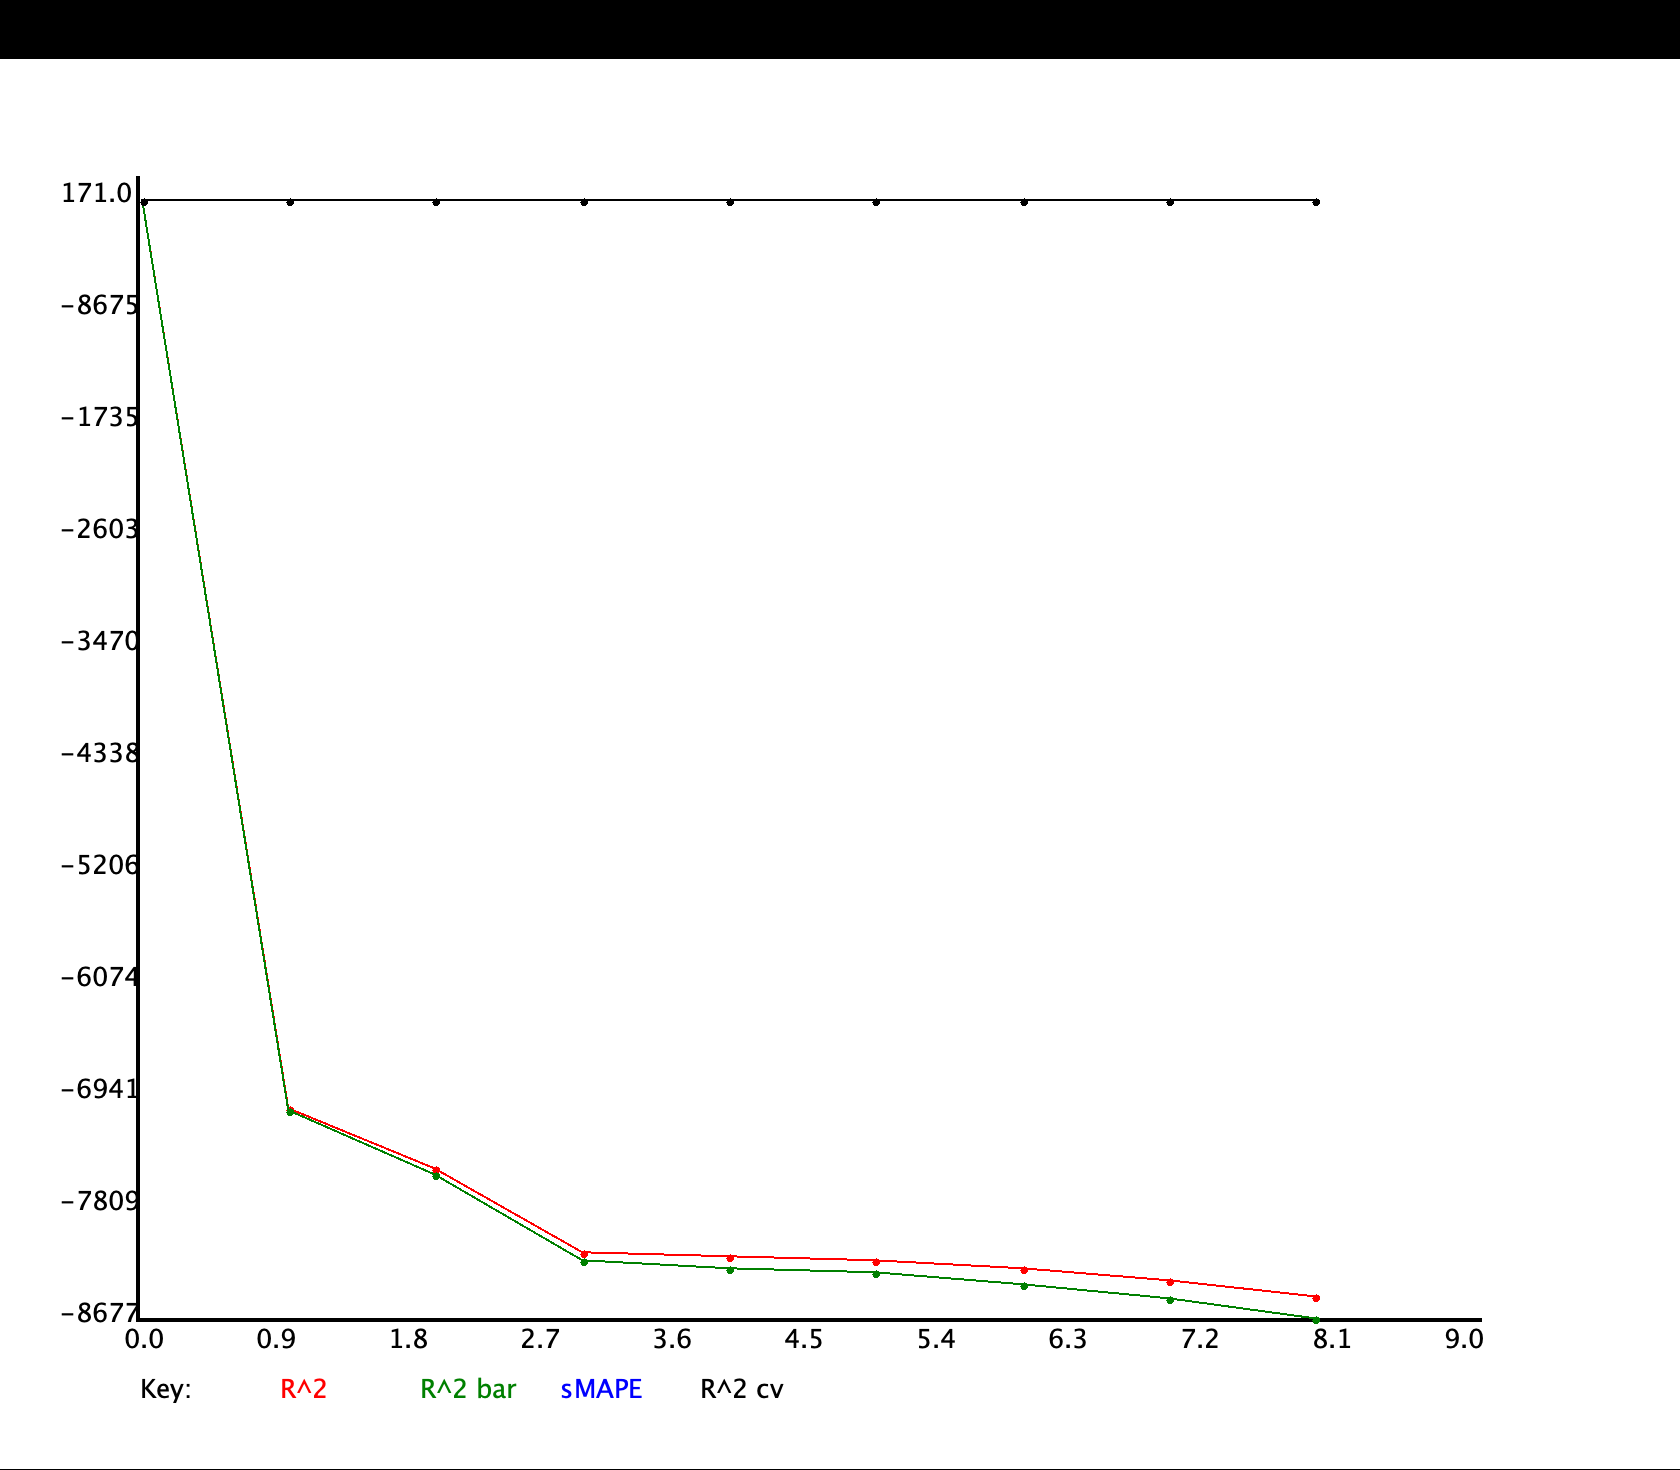
\includegraphics[width=\textwidth]{../Auto_MPG_Scalation_Plots/Scalation_BoxCox_rSq_Backward.png}
     \end{subfigure}
     \hfill
     \begin{subfigure}[b]{0.4\textwidth}
         \centering
         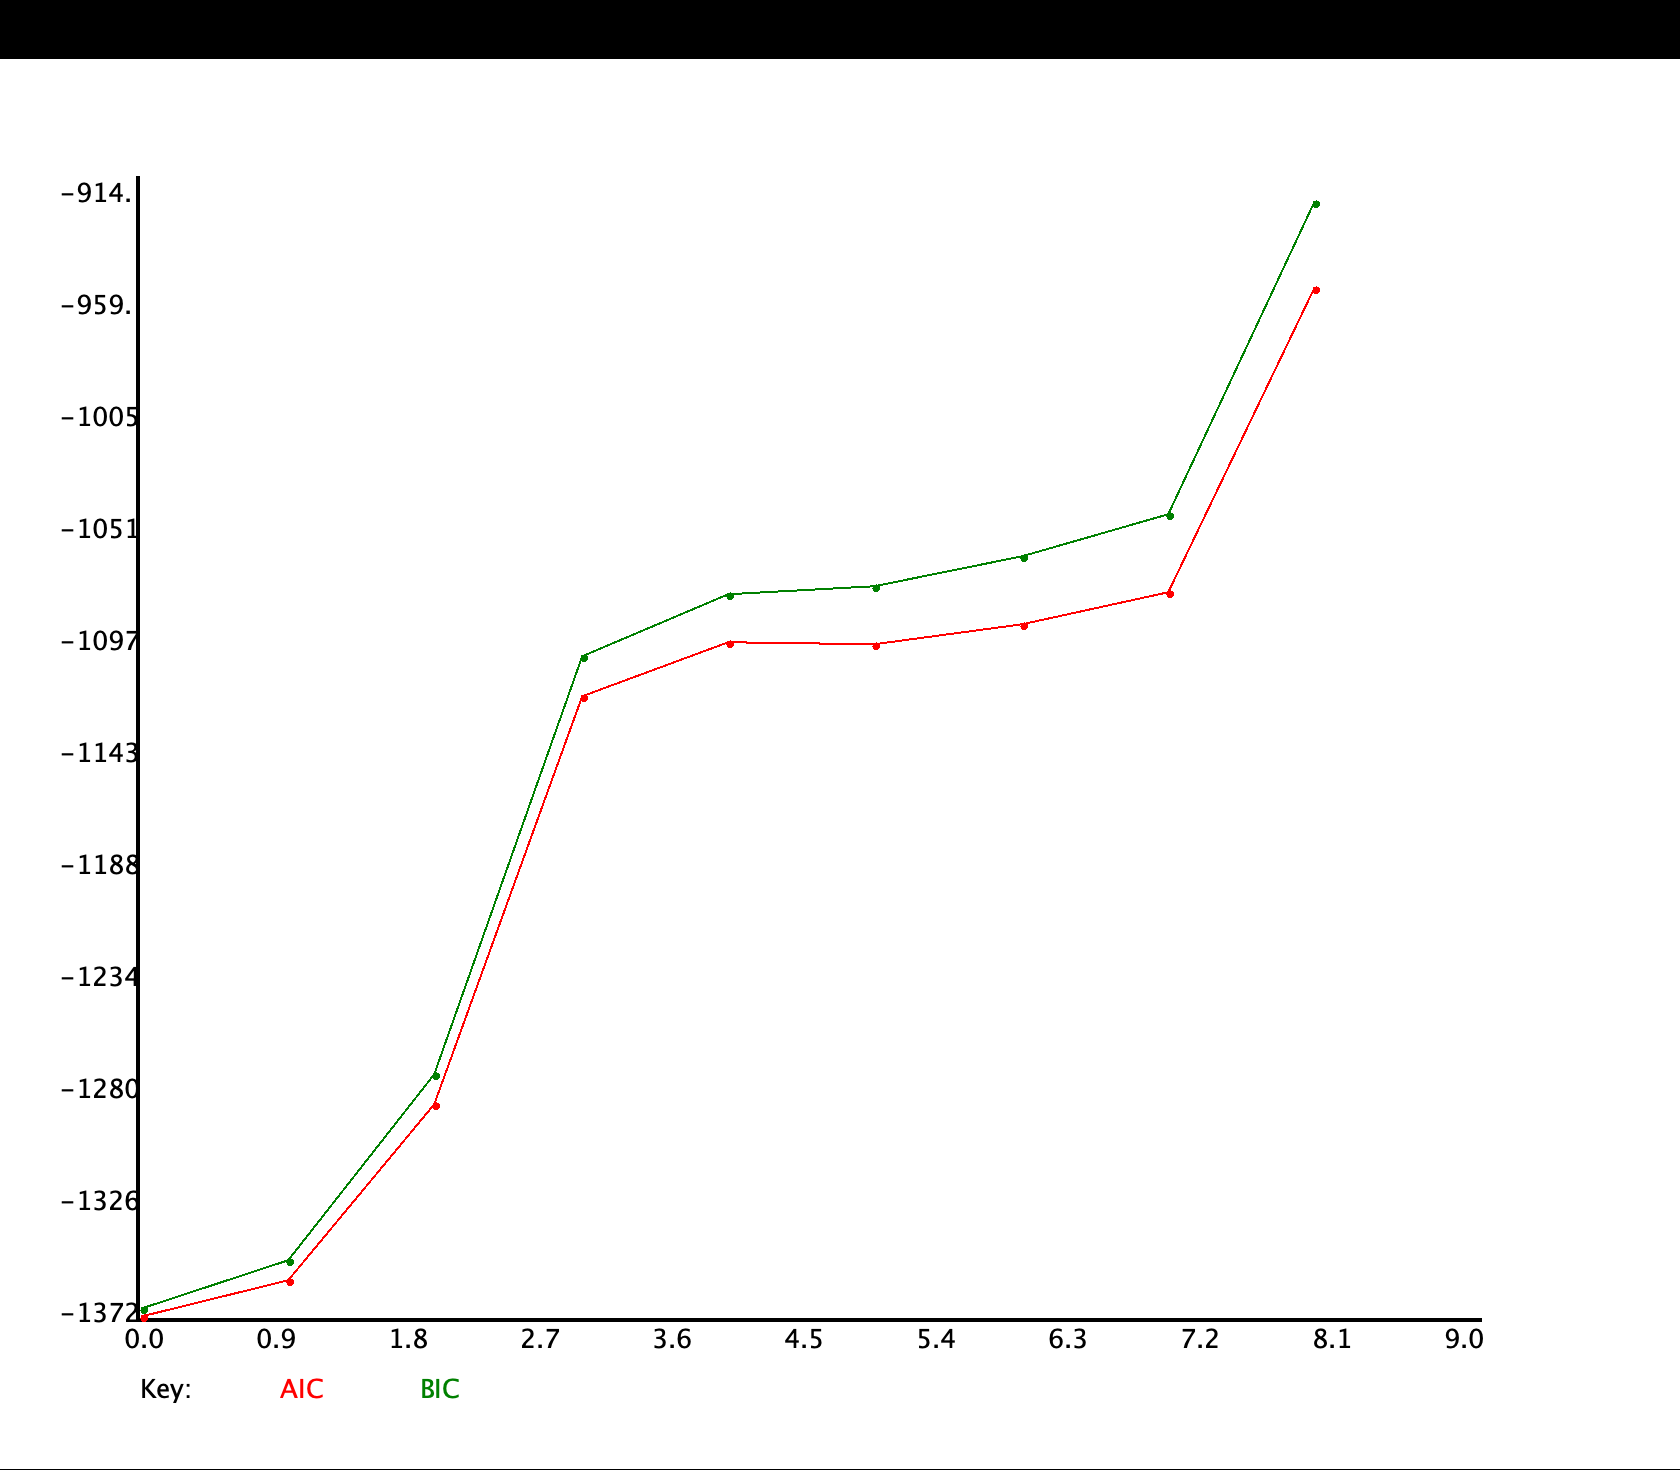
\includegraphics[width=\textwidth]{../Auto_MPG_Scalation_Plots/Scalation_BoxCox_AIC_BIC_Backward.png}
     \end{subfigure}

     \vspace{10pt} % Add some vertical spacing between rows

     % Second Row
     \begin{subfigure}[b]{0.49\textwidth}
         \centering
         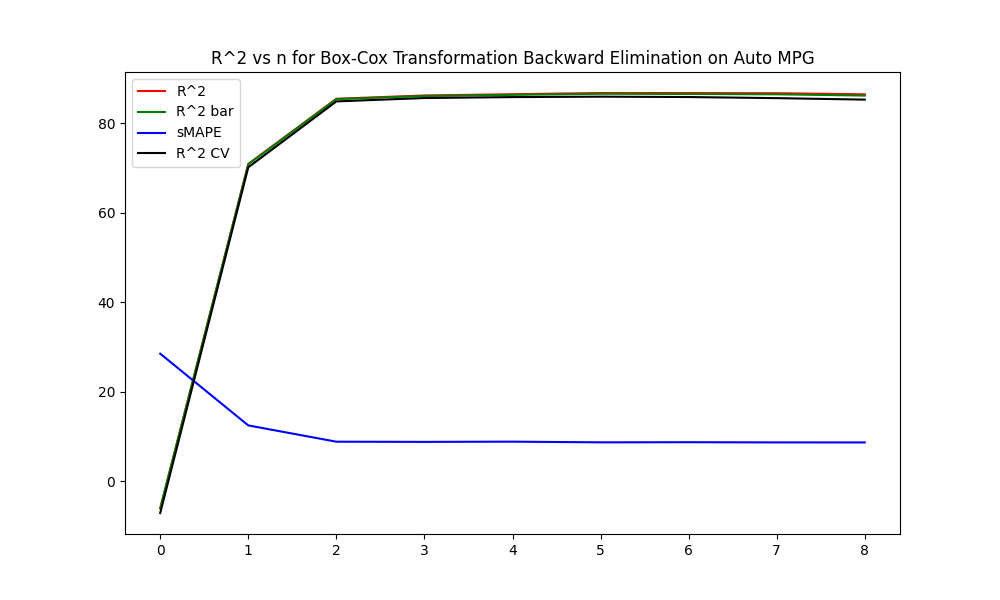
\includegraphics[width=\textwidth]{../Auto_MPG_Statsmodels_Plots/Statsmodels_BoxCox_rSq_Backward.png}
     \end{subfigure}
     \hfill
     \begin{subfigure}[b]{0.49\textwidth}
         \centering
         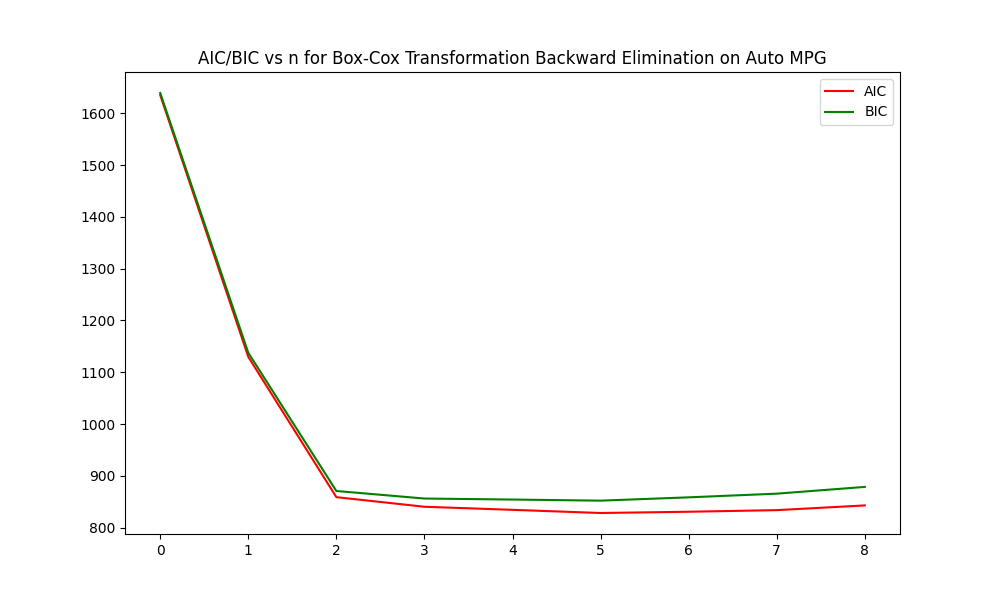
\includegraphics[width=\textwidth]{../Auto_MPG_Statsmodels_Plots/Statsmodels_BoxCox_AIC_BIC_Backward.png}
     \end{subfigure}
     
     \caption{Auto MPG Box-Cox Transformation Reversed Backward Elimination Quality of Fit Metrics\\ Top Left: Scalation $R^2$, Top Right: Scalation AIC/BIC\\ Bottom Left: Statsmodels $R^2$, Bottom Right: Statsmodels AIC/BIC}
     \label{fig:Auto MPG Box-Cox Transformation Reversed Backward Elimination Quality of Fit Metrics}
\end{figure}

Scalation Stepwise Selection: intercept

Statsmodels Stepwise Selection: intercept, weight, model year, horsepower, origin 2, origin 3

\begin{figure}[H]
     \centering
     \captionsetup{justification=centering}
%     % First Row
%     \begin{subfigure}[b]{0.4\textwidth}
%         \centering
%         %
\includegraphics[width=\textwidth]{../Auto_MPG_Scalation_Plots/Scalation_BoxCox_rSq_Stepwise.png}
%     \end{subfigure}
%     \hfill
%     \begin{subfigure}[b]{0.4\textwidth}
%         \centering
%         %
\includegraphics[width=\textwidth]{../Auto_MPG_Scalation_Plots/Scalation_BoxCox_AIC_BIC_Stepwise.png}
%     \end{subfigure}
%
%     \vspace{10pt} % Add some vertical spacing between rows

     % Second Row
     \begin{subfigure}[b]{0.49\textwidth}
         \centering
         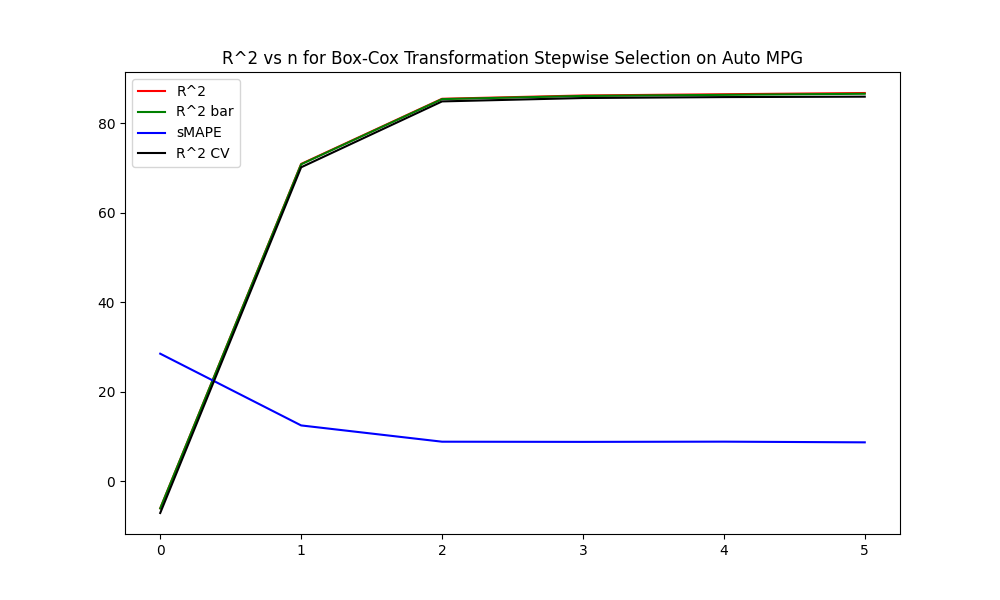
\includegraphics[width=\textwidth]{../Auto_MPG_Statsmodels_Plots/Statsmodels_BoxCox_rSq_Stepwise.png}
     \end{subfigure}
     \hfill
     \begin{subfigure}[b]{0.49\textwidth}
         \centering
         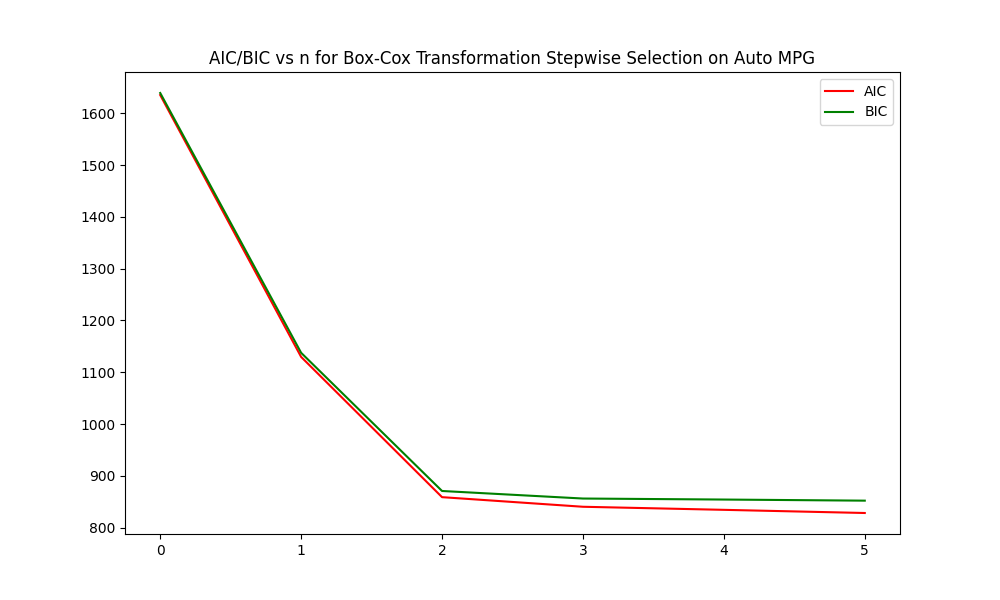
\includegraphics[width=\textwidth]{../Auto_MPG_Statsmodels_Plots/Statsmodels_BoxCox_AIC_BIC_Stepwise.png}
     \end{subfigure}
     
     \caption{Auto MPG Box-Cox Transformation Stepwise Selection Quality of Fit Metrics\\ Left: Statsmodels $R^2$, Right: Statsmodels AIC/BIC}
     \label{fig:Auto MPG Box-Cox Transformation Stepwise Selection Quality of Fit Metrics}
\end{figure}

\subsection{Order 2 Polynomial Regression}

\subsubsection{Quality of Fit}

Scalation Auto MPG Order 2 Polynomial Lambda Used: $0.0000025$

\noindent Statsmodels Auto MPG Order 2 Polynomial alpha Used: $0.00015$

\begin{figure}[H]
     \centering
     \captionsetup{justification=centering}
     % First Row
     \begin{subfigure}[b]{0.4\textwidth}
         \centering
         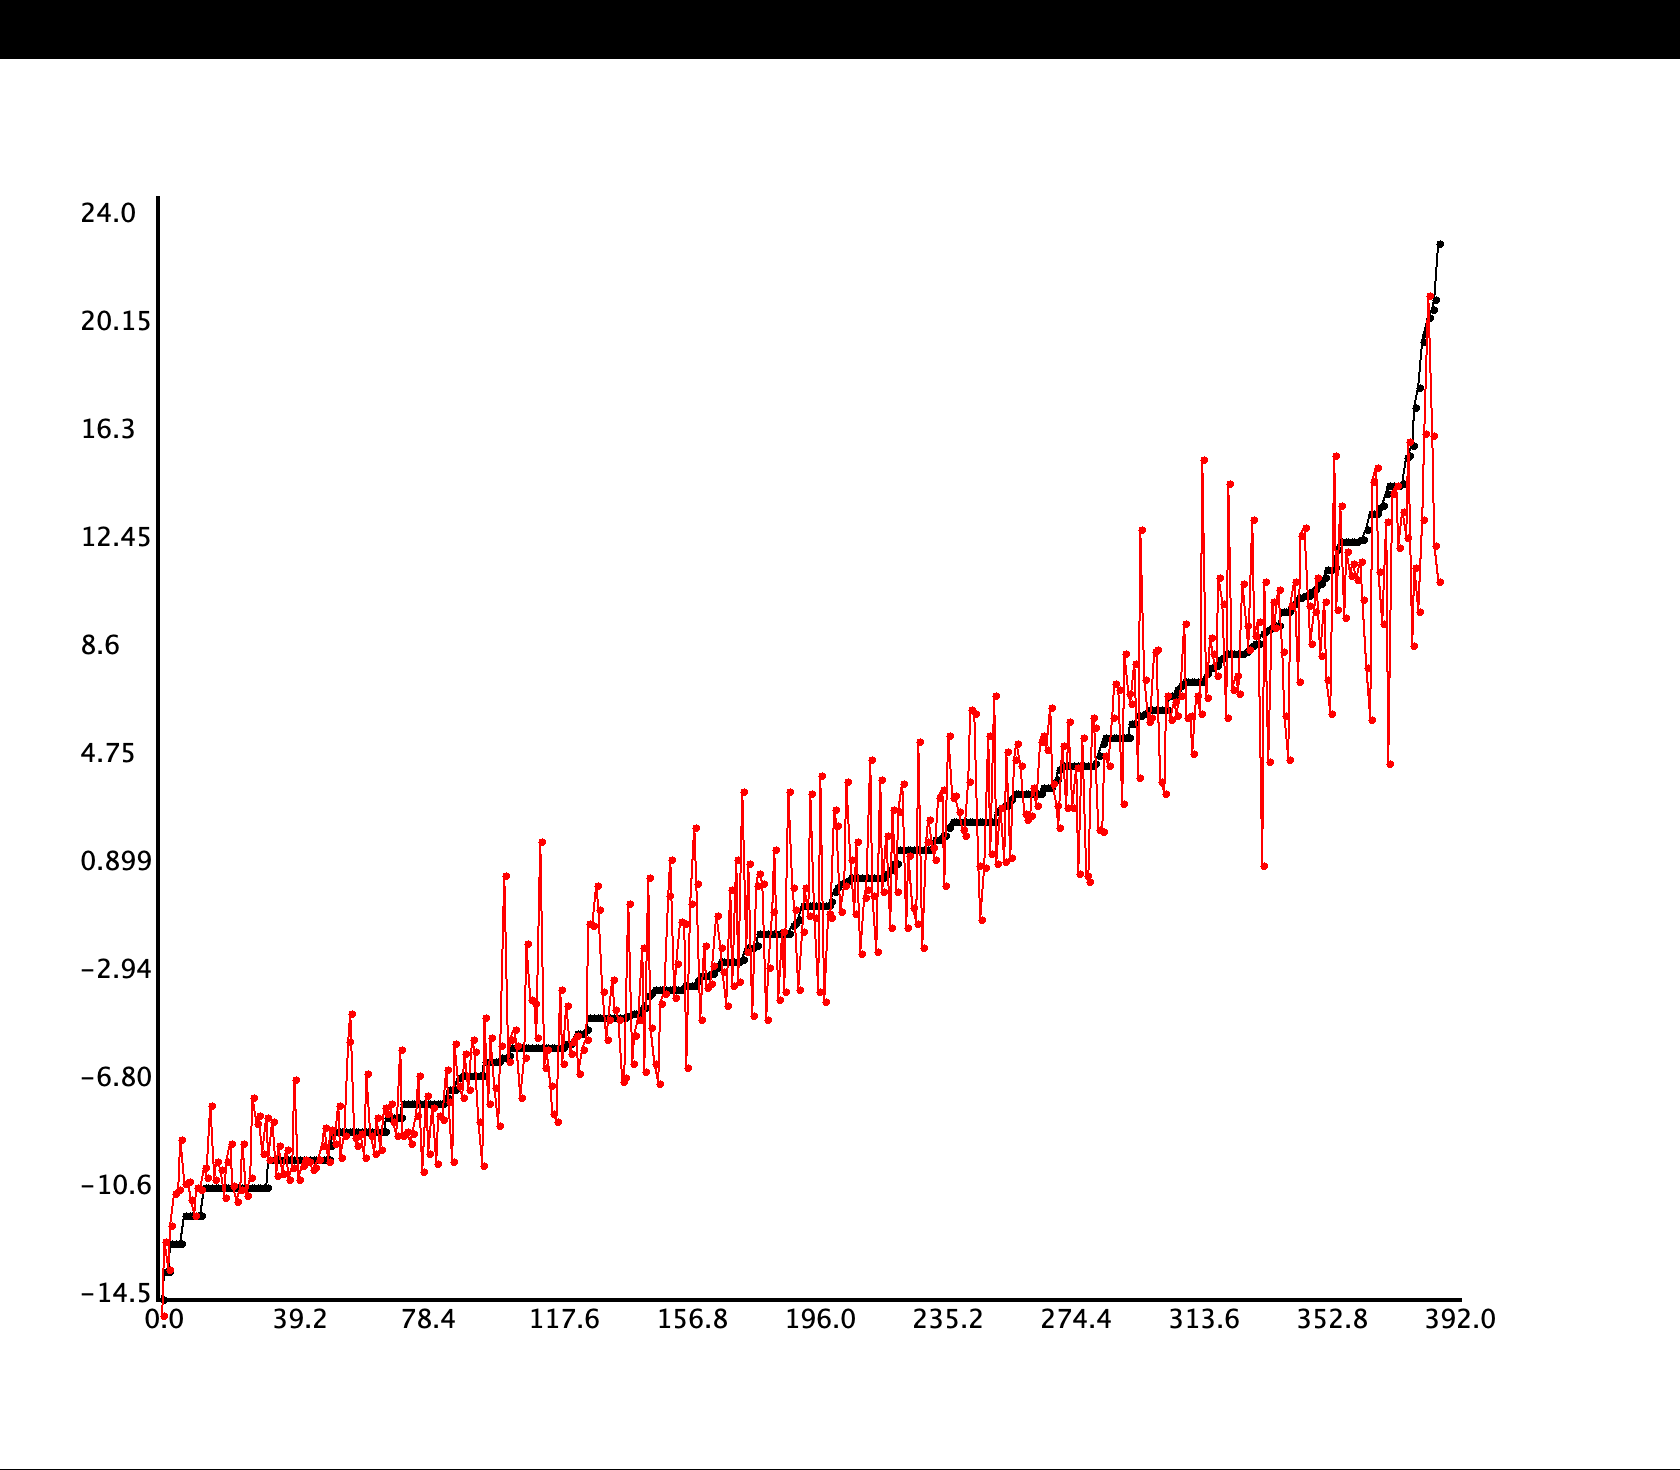
\includegraphics[width=\textwidth]{../Auto_MPG_Scalation_Plots/Scalation_Order2Reg_In_Sample.png}
     \end{subfigure}
     \hfill
     \begin{subfigure}[b]{0.4\textwidth}
         \centering
         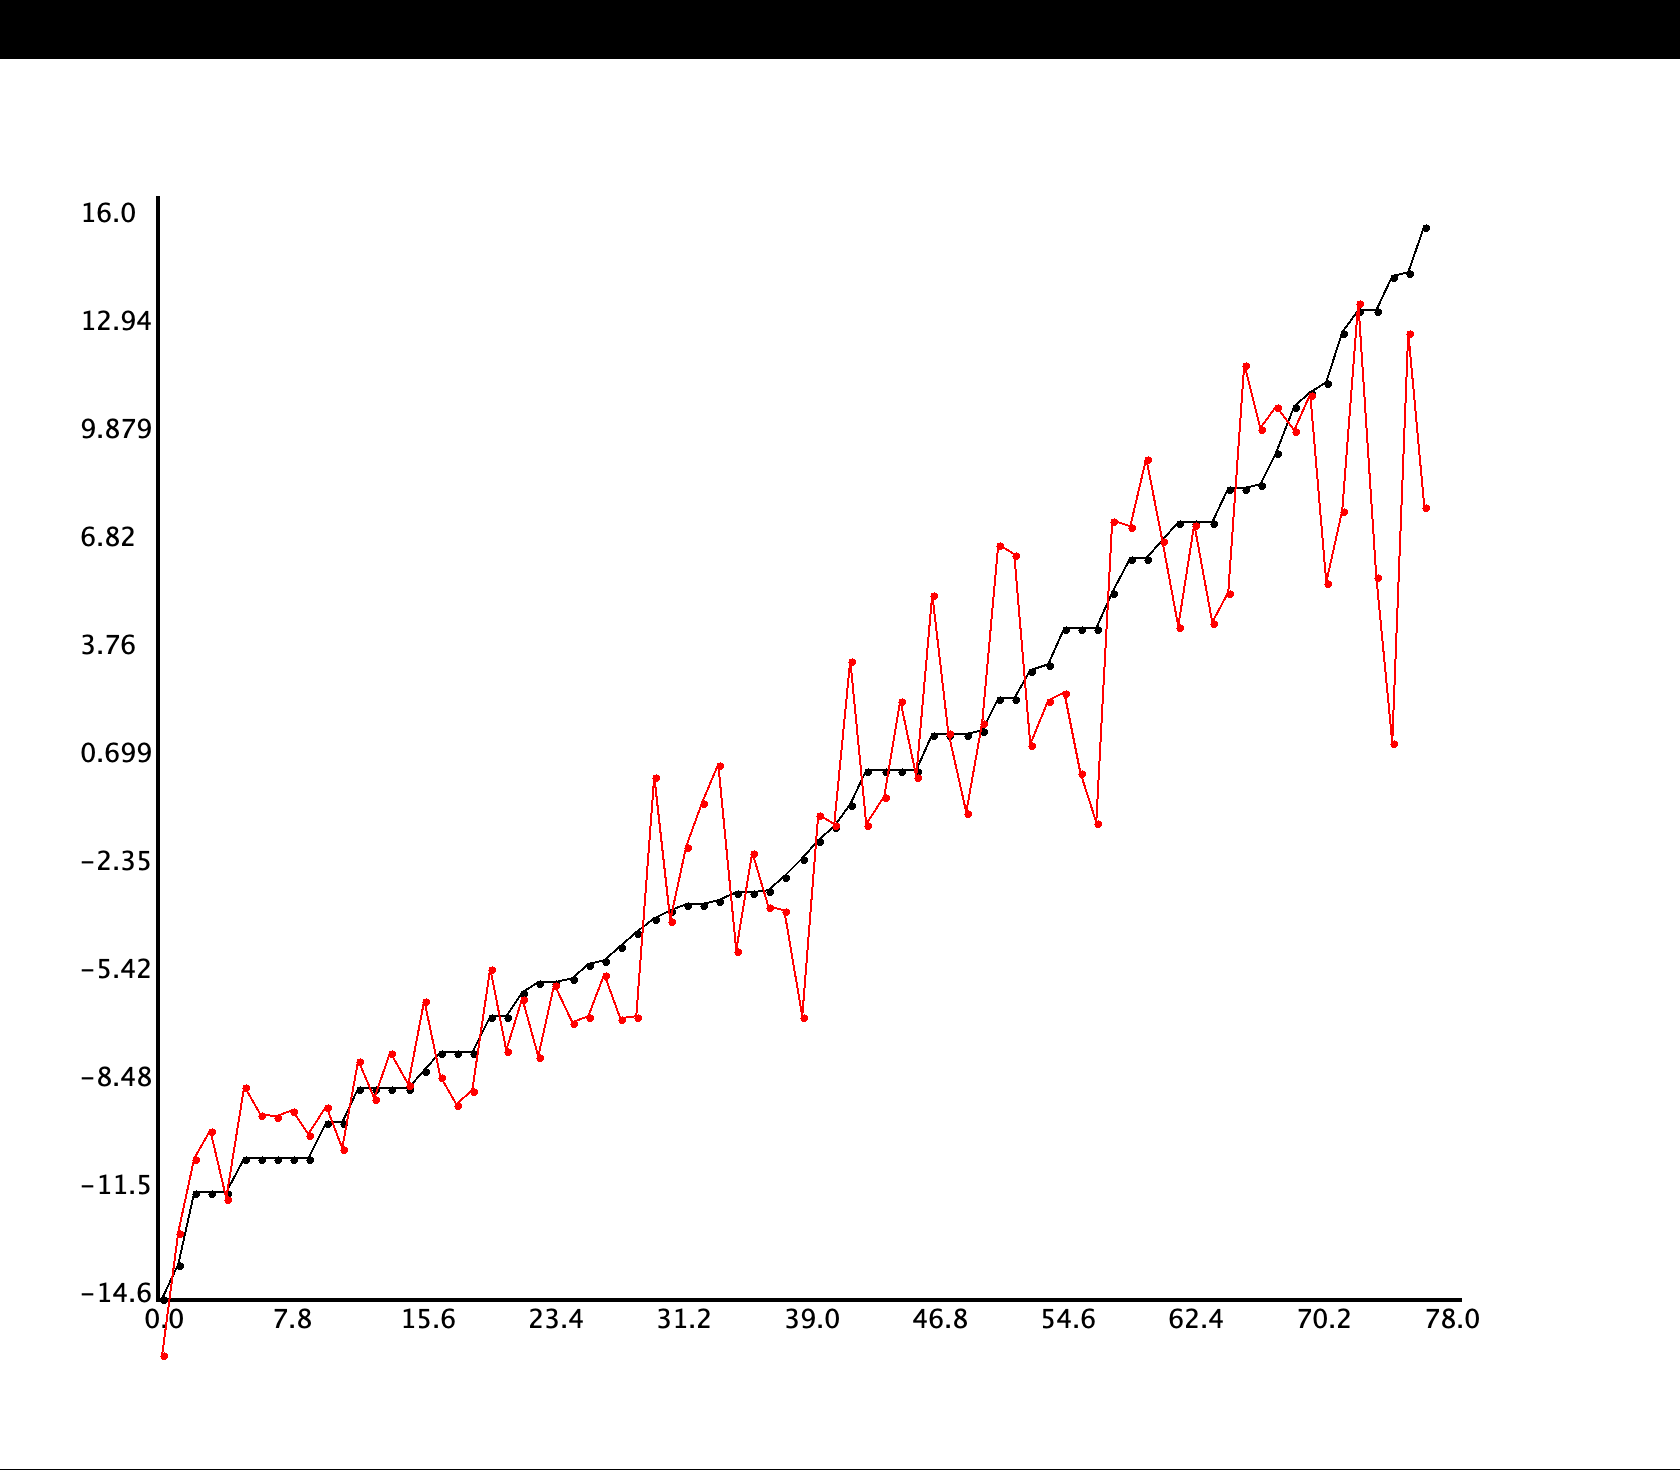
\includegraphics[width=\textwidth]{../Auto_MPG_Scalation_Plots/Scalation_Order2Reg_80_20.png}
     \end{subfigure}

     \vspace{10pt} % Add some vertical spacing between rows

     % Second Row
     \begin{subfigure}[b]{0.49\textwidth}
         \centering
         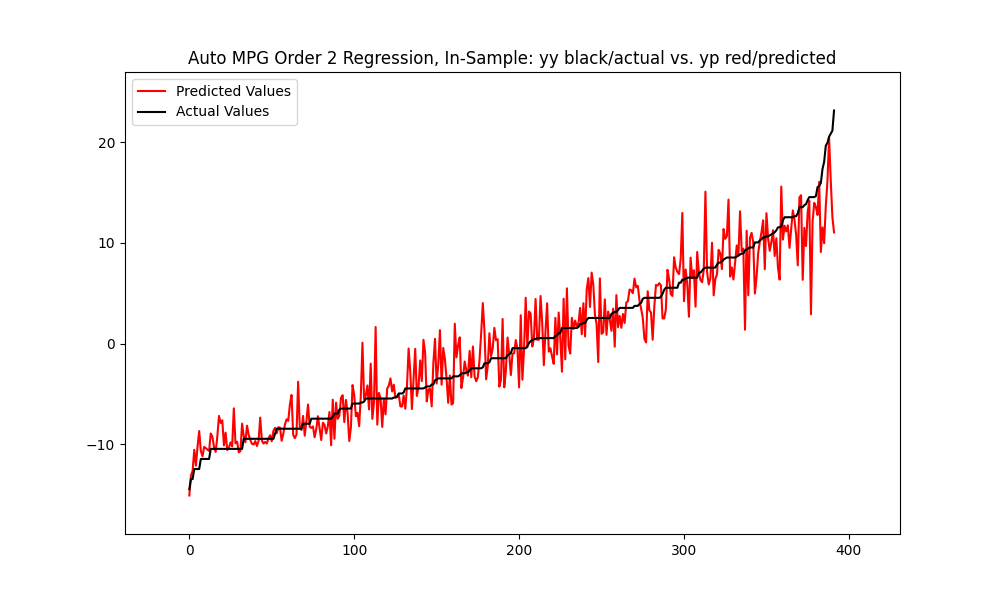
\includegraphics[width=\textwidth]{../Auto_MPG_Statsmodels_Plots/Statsmodels_Order2Reg_In_Sample.png}
     \end{subfigure}
     \hfill
     \begin{subfigure}[b]{0.49\textwidth}
         \centering
         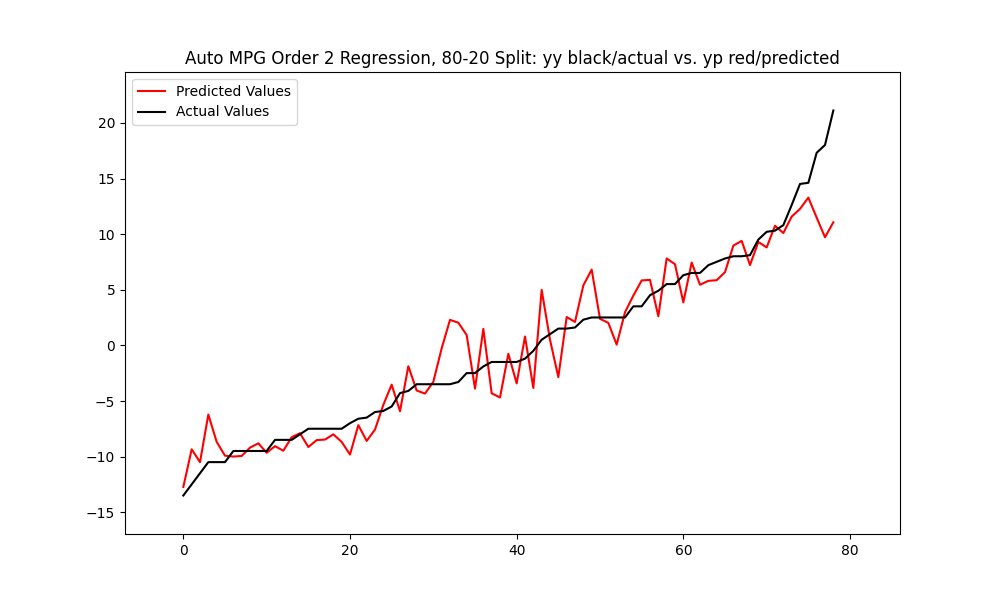
\includegraphics[width=\textwidth]{../Auto_MPG_Statsmodels_Plots/Statsmodels_Order2Reg_80_20.png}
     \end{subfigure}
     
     \caption{Auto MPG Order 2 Polynomial Regression Plots\\ Top Left: Scalation In-Sample, Top Right: Scalation Out-of-Sample\\ Bottom Left: Statsmodels In-Sample, Bottom Right: Statsmodels Out-of-Sample\\ black: actual y-values, red: predicted y-values}
     \label{fig:Auto MPG Order 2 Polynomial Regression Plots}
\end{figure}

\begin{table}[H]
\centering
\caption{Scalation - Auto MPG Order 2 Polynomial Regression}
\label{tab:Scalation - Auto MPG Order 2 Polynomial Regression}
\begin{tabular}{|c|c|c|} \hline 
Metric & In-Sample & 80-20 Split \\ \hline \hline 
rSq &0.901459 & 0.859902 \\ \hline 
rSqBar &0.887669 &      0.840296 \\ \hline 
sst &23819.0 &  4731.23 \\ \hline 
sse &2347.15 &  662.838 \\ \hline 
sde &2.45009 &  2.90243 \\ \hline 
mse0 &5.98764 & 8.49792 \\ \hline 
rmse &2.44696 & 2.91512 \\ \hline 
mae &1.74746 &  1.99920 \\ \hline 
smape &48.3661 &        50.7296 \\ \hline 
m &392.000 &    78.0000 \\ \hline 
dfr &48.0000 &  48.0000 \\ \hline 
df &343.000 &   343.000 \\ \hline 
fStat &65.3703 &        43.8600 \\ \hline 
aic &-809.004 & -96.1394 \\ \hline 
bic &-614.413 & 19.3393 \\ \hline 
\end{tabular}
\end{table}

\begin{table}[H]
\centering
\caption{Statsmodels - Auto MPG Order 2 Polynomial Regression}
\label{tab:Statsmodels - Auto MPG Order 2 Polynomial Regression}
\begin{tabular}{|c|c|c|}\hline
Metric & In-Sample & 80-20 Split \\ \hline \hline
rSq & 0.8990 & 0.8913 \\ \hline
rSqBar & 0.8852 & 0.7264 \\ \hline
sst & 23818.9935 & 4910.2699 \\ \hline
sse & 2405.3652 & 533.9271 \\ \hline
sde & 2.6443 & 4.1501 \\ \hline
mse0 & 6.1361 & 6.7586 \\ \hline
rmse & 2.4771 & 2.5997 \\ \hline
mae & 1.7742 & 1.8831 \\ \hline
smape & 47.7432 & 47.8555 \\ \hline
m & 392.0000 & 79.0000 \\ \hline
dfr & 48.0000 & 48.0000 \\ \hline
df & 344.0000 & 31.0000 \\ \hline
fStat & 63.8008 & 5.2936 \\ \hline
aic & 807.1645 & 246.9541 \\ \hline
bic & 997.7851 & 360.6876 \\ \hline
\end{tabular}
\end{table}

\begin{table}[H]
\centering
\caption{Scalation - Auto MPG Order 2 Polynomial Regression CV}
\label{tab:Scalation - Auto MPG Order 2 Polynomial Regression CV}
\begin{tabular}{|c|c|c|c|c|c|}\hline
Metric & num folds & min & max & mean & stdev \\ \hline \hline
rSq & 5 & 0.843 & 0.895 & 0.865 & 0.020 \\ \hline
rSqBar & 5 & 0.821 & 0.881 & 0.846 & 0.022 \\ \hline
sst & 5 & 3962.818 & 5671.580 & 4700.481 & 620.767 \\ \hline
sse & 5 & 512.429 & 702.036 & 628.878 & 76.157 \\ \hline
sde & 5 & 2.541 & 2.990 & 2.823 & 0.187 \\ \hline
mse0 & 5 & 6.570 & 9.000 & 8.063 & 0.976 \\ \hline
rmse & 5 & 2.563 & 3.000 & 2.835 & 0.176 \\ \hline
mae & 5 & 1.893 & 2.269 & 2.038 & 0.142 \\ \hline
smape & 5 & 49.914 & 59.190 & 52.629 & 3.785 \\ \hline
m & 5 & 78.000 & 78.000 & 78.000 & 0.000 \\ \hline
dfr & 5 & 48.000 & 48.000 & 48.000 & 0.000 \\ \hline
df & 5 & 343.000 & 343.000 & 343.000 & 0.000 \\ \hline
fStat & 5 & 38.379 & 61.057 & 46.760 & 8.718 \\ \hline
aic & 5 & -98.496 & -87.096 & -94.098 & 4.579 \\ \hline
bic & 5 & 16.983 & 28.382 & 21.381 & 4.579 \\ \hline
\end{tabular}
\end{table}

\begin{table}[H]
\centering
\caption{Statsmodels - Auto MPG Order 2 Polynomial Regression CV}
\label{tab:Statsmodels - Auto MPG Order 2 Polynomial Regression CV}
\begin{tabular}{|c|c|c|c|c|c|}\hline
Metric & num folds & min & max & mean & stdev \\ \hline \hline
rSq & 5 & 0.8264 & 0.9213 & 0.8691 & 0.0334 \\ \hline
rSqBar & 5 & 0.5545 & 0.7981 & 0.6666 & 0.0859 \\ \hline
sst & 5 & 3880.9704 & 5093.9237 & 4721.1782 & 441.3031 \\ \hline
sse & 5 & 400.7975 & 754.0760 & 607.1392 & 125.2835 \\ \hline
sde & 5 & 3.6551 & 5.0136 & 4.4435 & 0.4835 \\ \hline
mse0 & 5 & 5.1384 & 9.6676 & 7.7447 & 1.6055 \\ \hline
rmse & 5 & 2.2668 & 3.1093 & 2.7667 & 0.2996 \\ \hline
mae & 5 & 1.6558 & 2.2427 & 1.9847 & 0.2006 \\ \hline
smape & 5 & 38.2464 & 61.9974 & 52.2568 & 8.4141 \\ \hline
m & 5 & 78.0000 & 79.0000 & 78.4000 & 0.4899 \\ \hline
dfr & 5 & 48.0000 & 48.0000 & 48.0000 & 0.0000 \\ \hline
df & 5 & 30.0000 & 31.0000 & 30.4000 & 0.4899 \\ \hline
fStat & 5 & 2.9755 & 7.3184 & 4.5978 & 1.5619 \\ \hline
aic & 5 & 223.6663 & 272.9652 & 254.6013 & 17.6677 \\ \hline
bic & 5 & 336.7883 & 386.0872 & 367.9679 & 17.6910 \\ \hline
\end{tabular}
\end{table}

\subsubsection{Feature Selection}

Scalation Forward Selection: displacement, horsepower $\times$ acceleration, model year $\times$ model year, weight, weight $\times$ weight, weight $\times$ model year, acceleration, acceleration $\times$ origin 1, model year $\times$ origin 1, acceleration $\times$ acceleration, weight $\times$ acceleration, displacement $\times$ weight, horsepower, horsepower $\times$ model year, model year, origin 1, displacement $\times$ displacement, acceleration $\times$ model year, weight $\times$ origin 1, displacement $\times$ model year, displacement $\times$ origin 1, horsepower $\times$ origin 2, cylinders $\times$ origin 3, weight $\times$ origin 2, displacement $\times$ origin 3, horsepower $\times$ weight, displacement $\times$ horsepower, displacement $\times$ acceleration, acceleration $\times$ origin 3, model year $\times$ origin 2, cylinders $\times$ origin 2, horsepower $\times$ horsepower, horsepower $\times$ origin 3, cylinders $\times$ horsepower, cylinders $\times$ acceleration, cylinders $\times$ model year, origin 2, cylinders $\times$ origin 1, cylinders $\times$ cylinders, cylinders $\times$ weight, origin 3, cylinders, model year $\times$ origin 3, weight $\times$ origin 3, horsepower $\times$ origin 1, displacement $\times$ cylinders, displacement $\times$ origin 2, acceleration $\times$ origin 2

Statsmodels Forward Selection: Null, weight, model year $\times$ model year, weight $\times$ weight, model year, horsepower $\times$ model year, horsepower, acceleration $\times$ origin 1, horsepower $\times$ origin 1, weight $\times$ origin 1, origin 1, acceleration $\times$ acceleration, model year $\times$ origin 1, horsepower $\times$ acceleration, acceleration $\times$ model year, acceleration, horsepower $\times$ horsepower, displacement $\times$ origin 1, displacement $\times$ weight, cylinders $\times$ acceleration, cylinders, displacement, displacement $\times$ model year, cylinders $\times$ horsepower, cylinders $\times$ cylinders, cylinders $\times$ weight, horsepower $\times$ weight, weight $\times$ model year, acceleration $\times$ origin 2, cylinders $\times$ origin 3, weight $\times$ origin 3, displacement $\times$ origin 2, cylinders $\times$ origin 2, model year $\times$ origin 2, origin 2, origin 3, cylinders $\times$ model year, displacement $\times$ cylinders, weight $\times$ origin 2, weight $\times$ acceleration, horsepower $\times$ origin 3, horsepower $\times$ origin 2, cylinders $\times$ origin 1, model year $\times$ origin 3, displacement $\times$ horsepower, displacement $\times$ displacement, acceleration $\times$ origin 3, displacement $\times$ acceleration, displacement $\times$ origin 3

\begin{figure}[H]
     \centering
     \captionsetup{justification=centering}
     % First Row
     \begin{subfigure}[b]{0.4\textwidth}
         \centering
         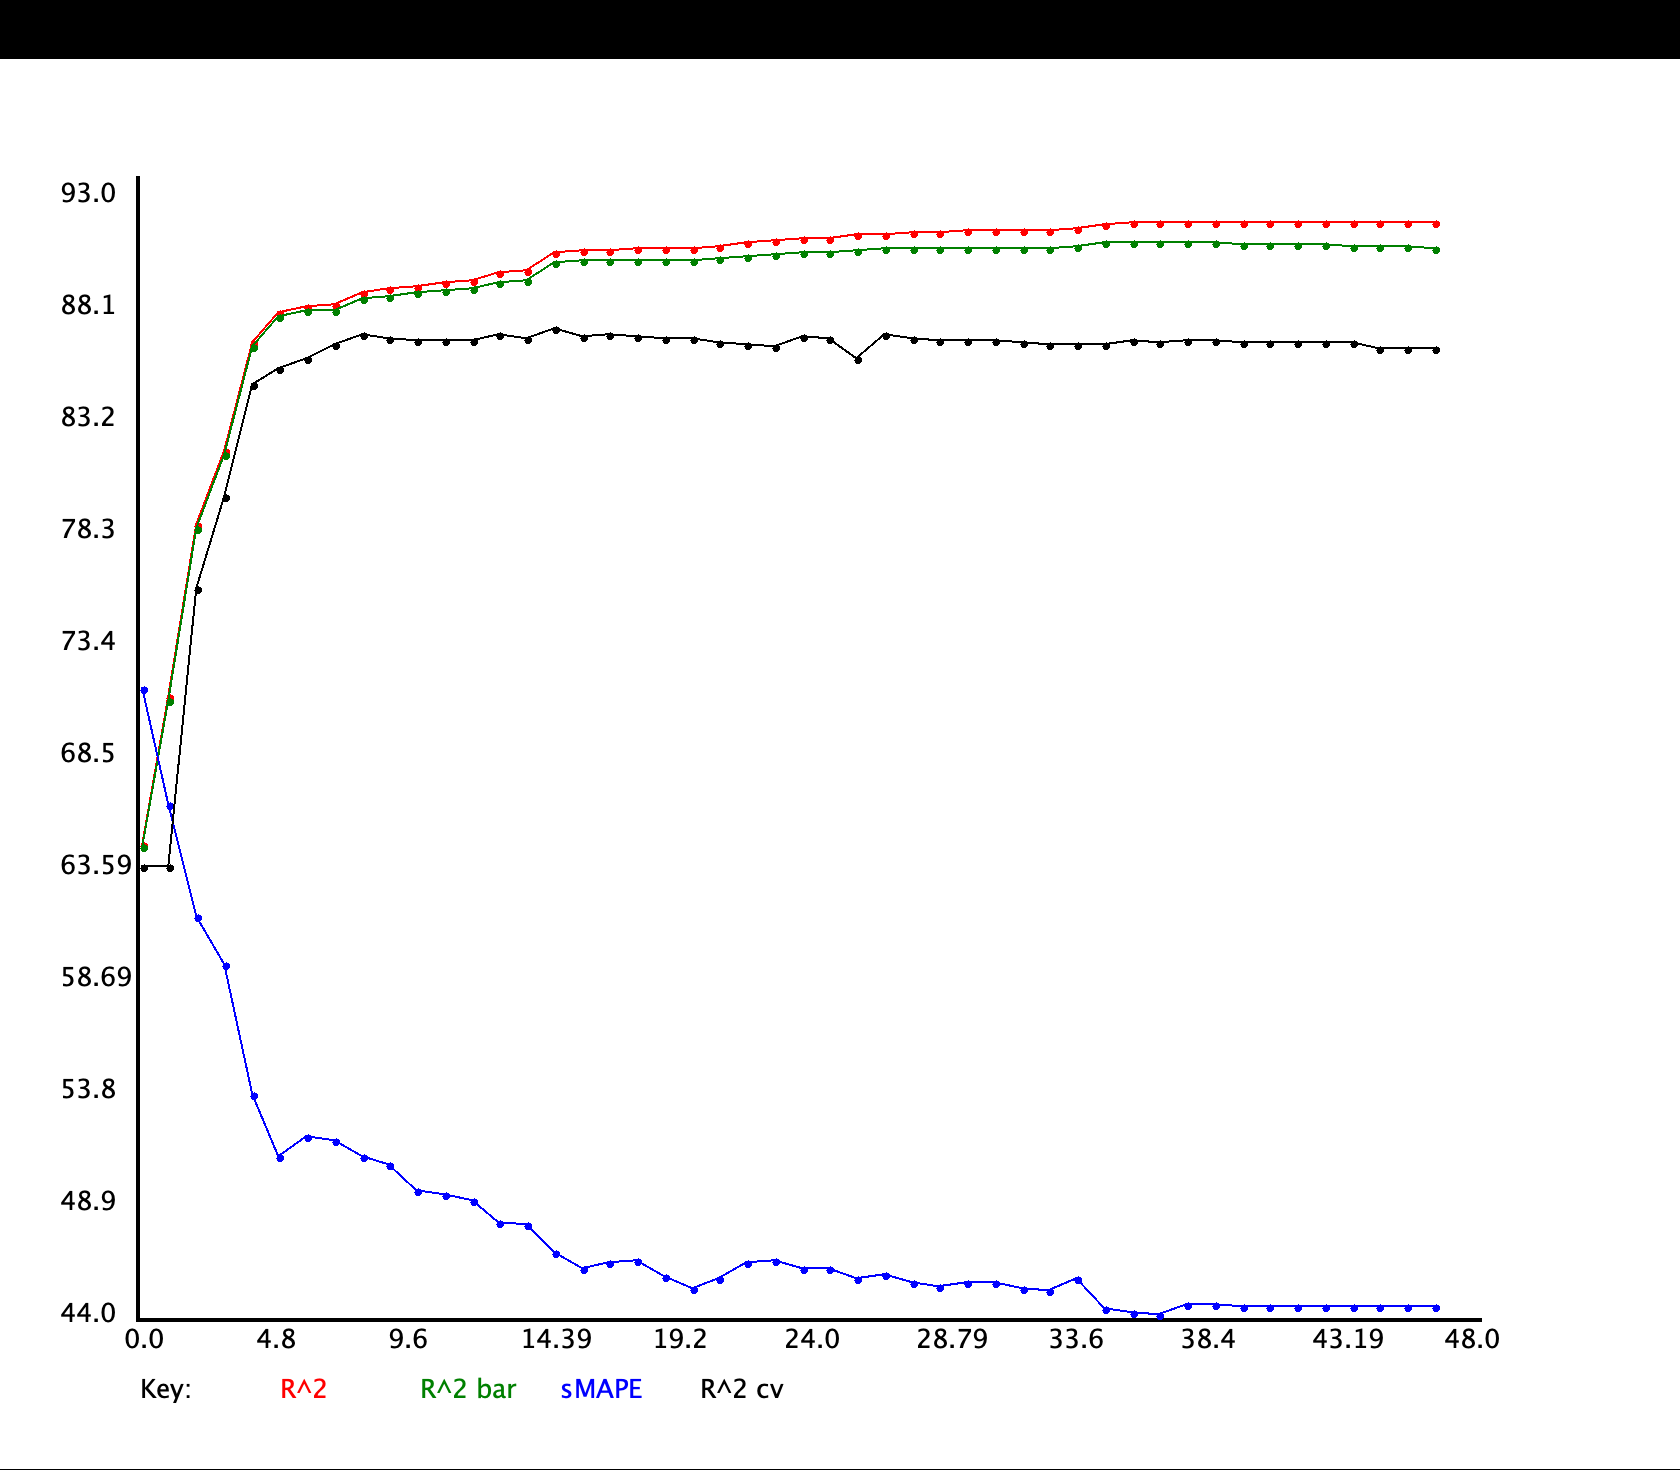
\includegraphics[width=\textwidth]{../Auto_MPG_Scalation_Plots/Scalation_Order2Reg_rSq_Forward.png}
     \end{subfigure}
     \hfill
     \begin{subfigure}[b]{0.4\textwidth}
         \centering
         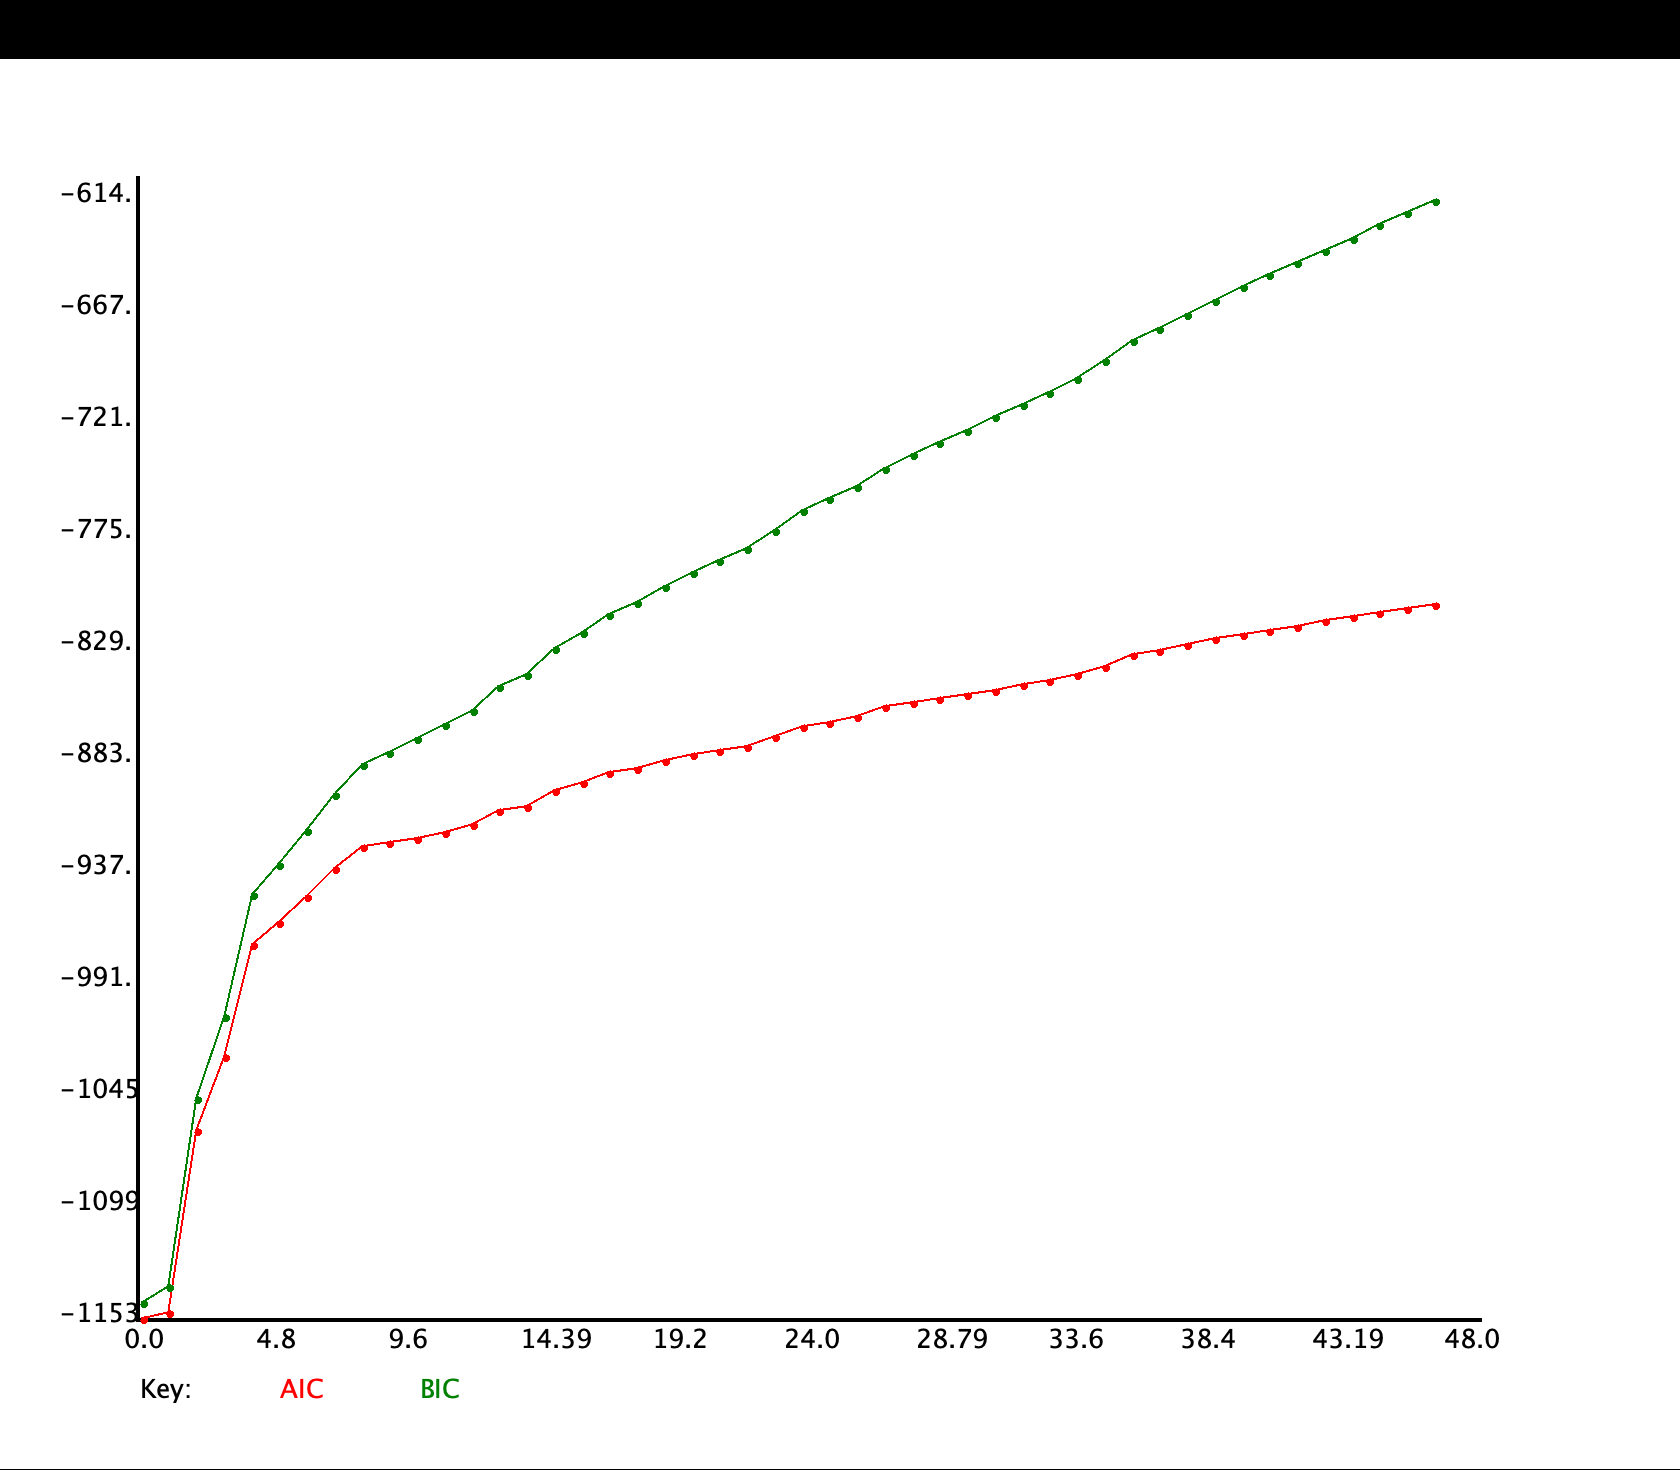
\includegraphics[width=\textwidth]{../Auto_MPG_Scalation_Plots/Scalation_Order2Reg_AIC_BIC_Forward.png}
     \end{subfigure}

     \vspace{10pt} % Add some vertical spacing between rows

     % Second Row
     \begin{subfigure}[b]{0.49\textwidth}
         \centering
         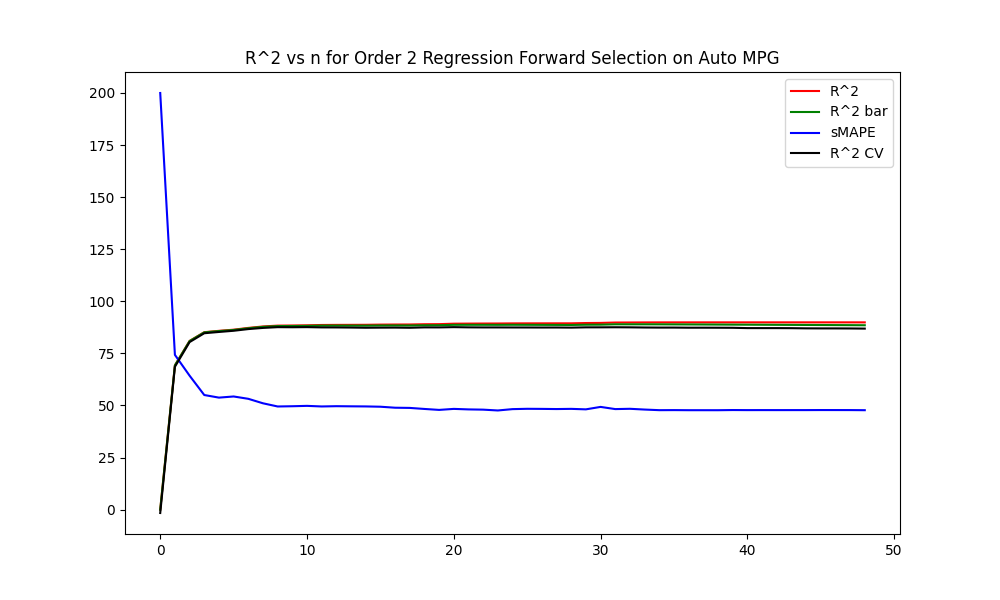
\includegraphics[width=\textwidth]{../Auto_MPG_Statsmodels_Plots/Statsmodels_Order2Reg_rSq_Forward.png}
     \end{subfigure}
     \hfill
     \begin{subfigure}[b]{0.49\textwidth}
         \centering
         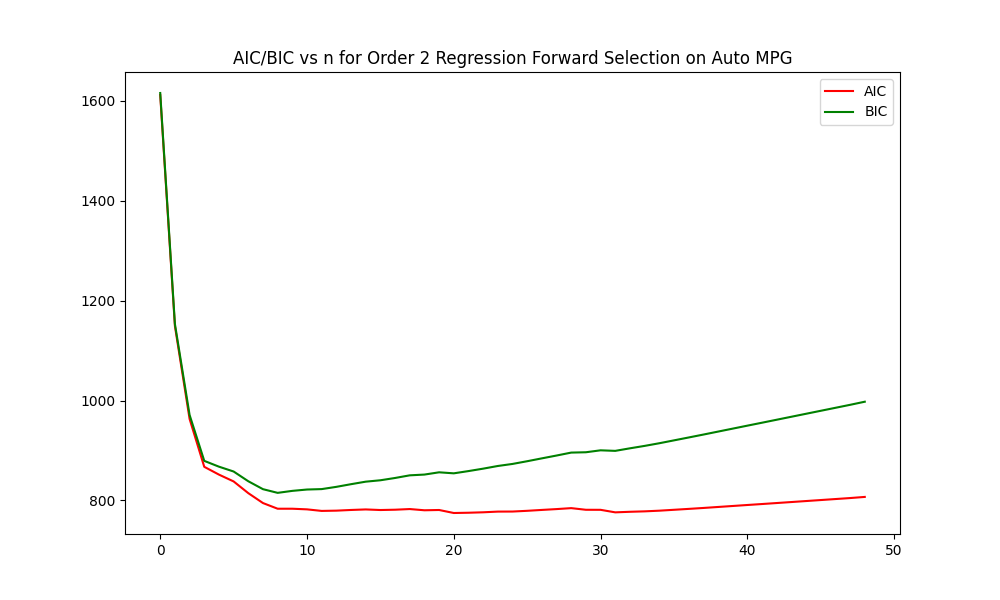
\includegraphics[width=\textwidth]{../Auto_MPG_Statsmodels_Plots/Statsmodels_Order2Reg_AIC_BIC_Forward.png}
     \end{subfigure}
     
     \caption{Auto MPG Order 2 Polynomial Regression Forward Selection Quality of Fit Metrics\\ Top Left: Scalation $R^2$, Top Right: Scalation AIC/BIC\\ Bottom Left: Statsmodels $R^2$, Bottom Right: Statsmodels AIC/BIC}
     \label{fig:Auto MPG Order 2 Polynomial Regression Forward Selection Quality of Fit Metrics}
\end{figure}

Scalation Backward Elimination Reversed: displacement, weight $\times$ model year, model year $\times$ model year, origin 1, displacement $\times$ weight, model year, acceleration $\times$ origin 2, acceleration $\times$ origin 3, horsepower $\times$ weight, acceleration, displacement $\times$ displacement, displacement $\times$ horsepower, cylinders $\times$ acceleration, cylinders $\times$ model year, model year $\times$ origin 3, cylinders $\times$ origin 3, cylinders $\times$ origin 1, weight $\times$ origin 2, weight $\times$ origin 1, horsepower, horsepower $\times$ acceleration, horsepower $\times$ horsepower, displacement $\times$ model year, cylinders $\times$ weight, acceleration $\times$ model year, cylinders $\times$ cylinders, model year $\times$ origin 1, weight $\times$ origin 3, origin 2, cylinders, displacement $\times$ origin 3, displacement $\times$ origin 1, weight $\times$ weight, displacement $\times$ acceleration, origin 3, horsepower $\times$ origin 2, cylinders $\times$ horsepower, acceleration $\times$ acceleration, horsepower $\times$ model year, weight $\times$ acceleration, horsepower $\times$ origin 1, cylinders $\times$ origin 2, model year $\times$ origin 2, weight, horsepower $\times$ origin 3, displacement $\times$ cylinders, displacement $\times$ origin 2, acceleration $\times$ origin 1

Statsmodels Backward Elimination Reversed: Null, weight, acceleration $\times$ model year, acceleration, displacement $\times$ weight, displacement $\times$ origin 1, weight $\times$ origin 3, displacement $\times$ origin 2, acceleration $\times$ origin 1, origin 1, cylinders $\times$ acceleration, cylinders, model year, model year $\times$ model year, horsepower $\times$ acceleration, model year $\times$ origin 1, cylinders $\times$ origin 2, model year $\times$ origin 2, cylinders $\times$ horsepower, horsepower $\times$ horsepower, cylinders $\times$ cylinders, weight $\times$ origin 2, cylinders $\times$ weight, displacement $\times$ model year, horsepower, horsepower $\times$ model year, origin 2, cylinders $\times$ origin 1, displacement, displacement $\times$ cylinders, origin 3, cylinders $\times$ model year, horsepower $\times$ origin 3, horsepower $\times$ origin 2, horsepower $\times$ origin 1, displacement $\times$ horsepower, displacement $\times$ displacement, weight $\times$ weight, model year $\times$ origin 3, acceleration $\times$ acceleration, horsepower $\times$ weight, weight $\times$ origin 1, displacement $\times$ acceleration, acceleration $\times$ origin 3, acceleration $\times$ origin 2, weight $\times$ acceleration, weight $\times$ model year, cylinders $\times$ origin 3, displacement $\times$ origin 3

\begin{figure}[H]
     \centering
     \captionsetup{justification=centering}
     % First Row
     \begin{subfigure}[b]{0.4\textwidth}
         \centering
         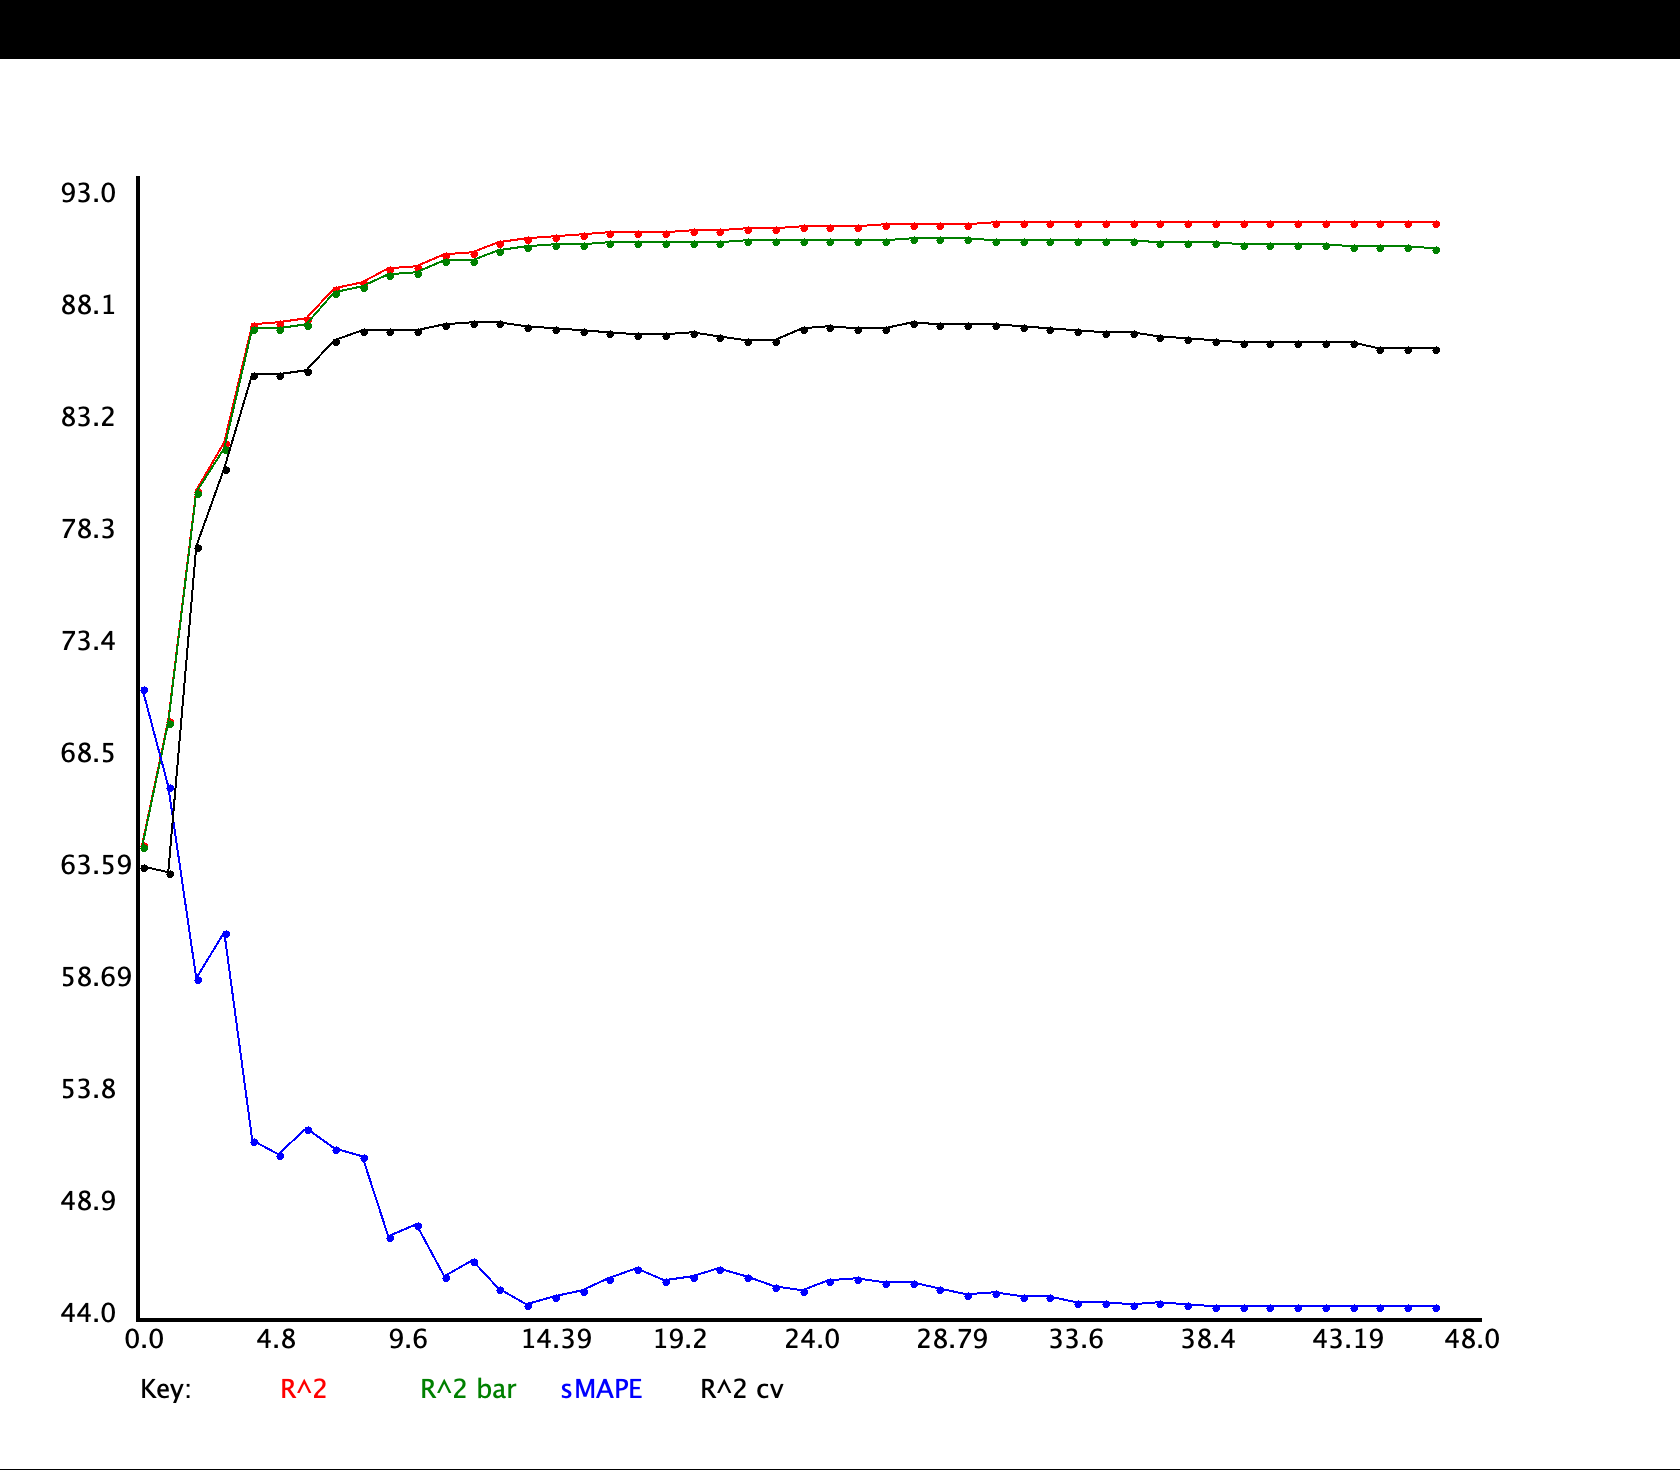
\includegraphics[width=\textwidth]{../Auto_MPG_Scalation_Plots/Scalation_Order2Reg_rSq_Backward.png}
     \end{subfigure}
     \hfill
     \begin{subfigure}[b]{0.4\textwidth}
         \centering
         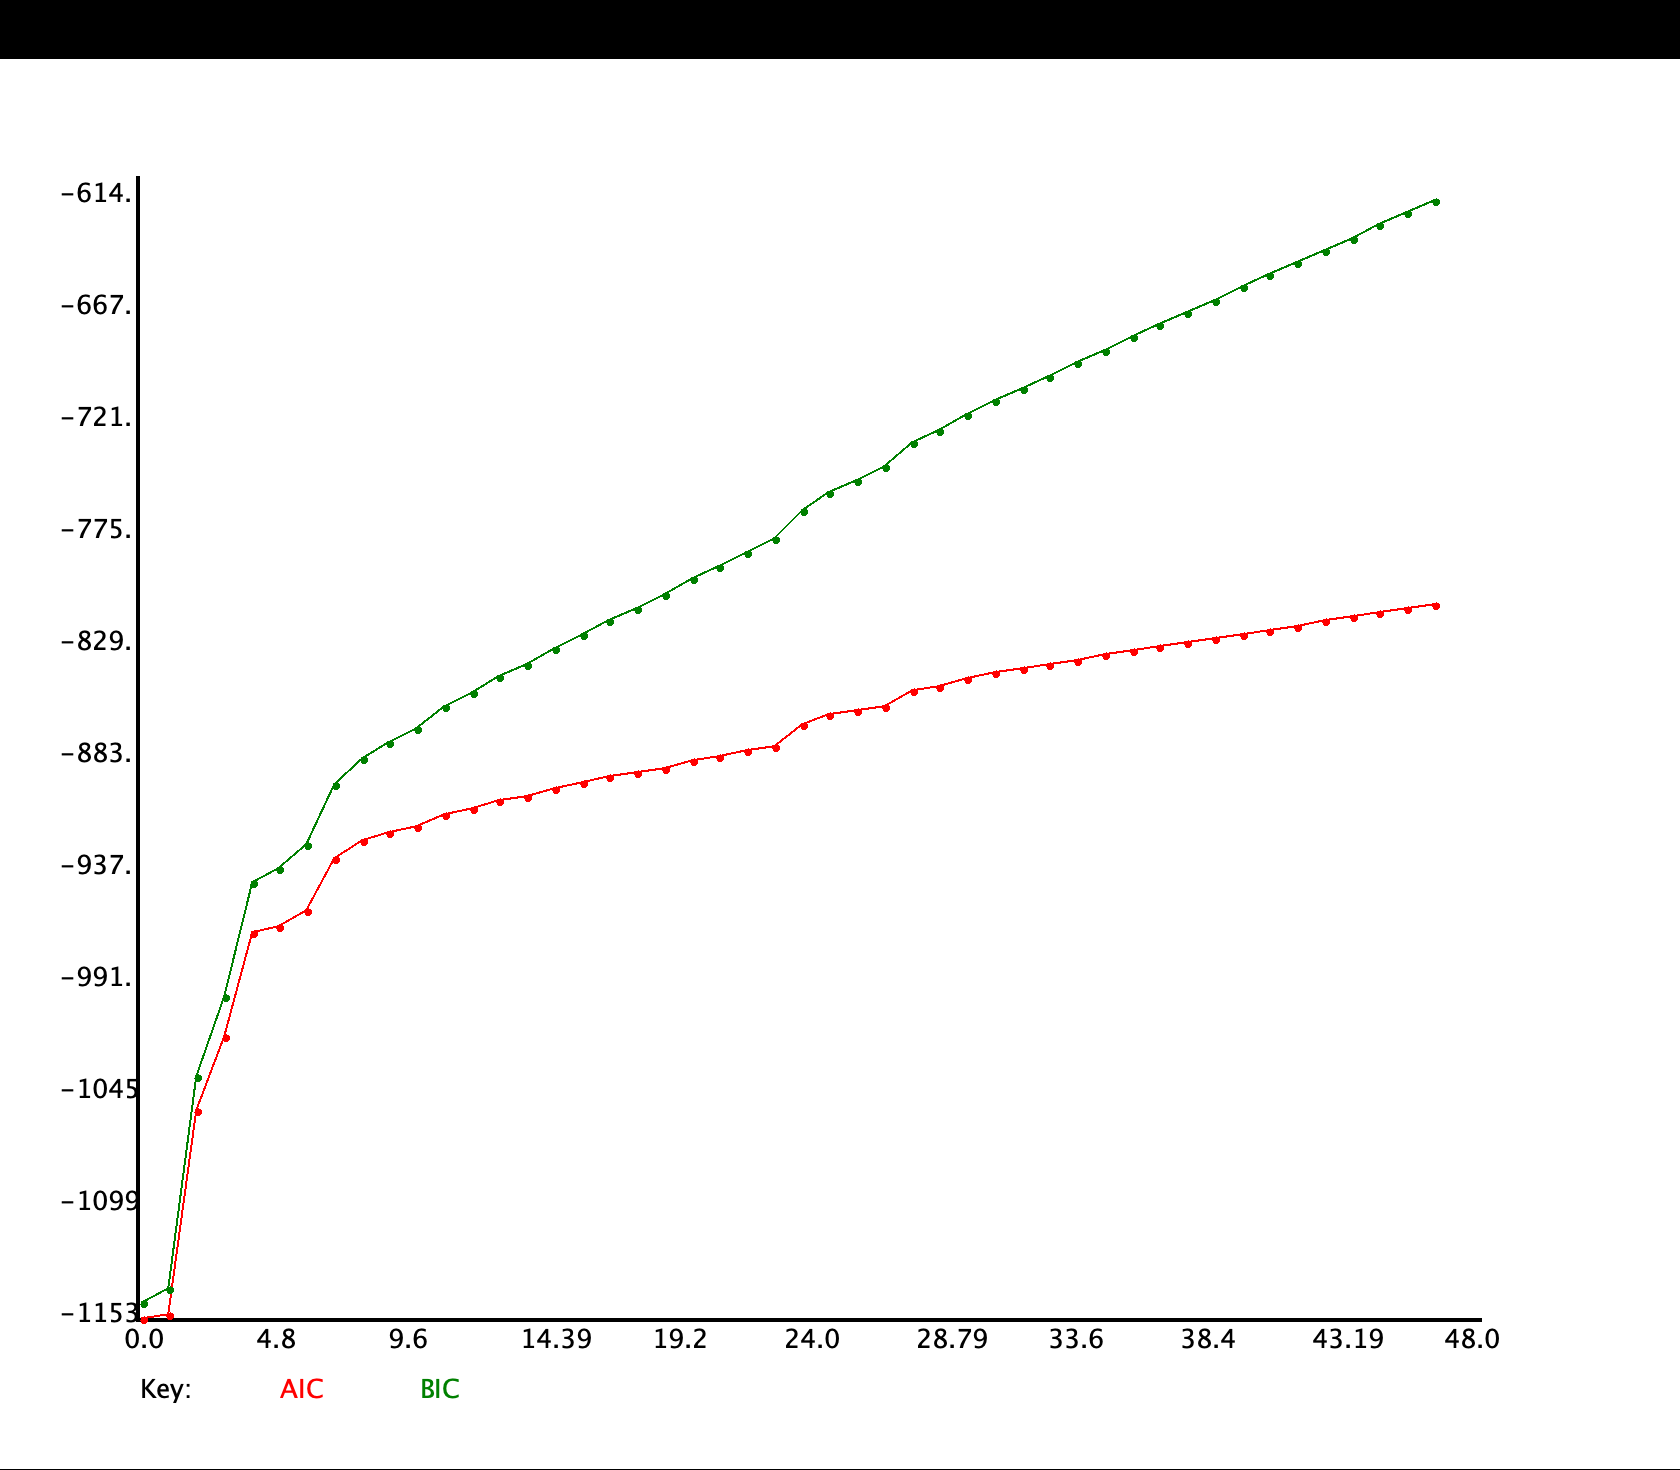
\includegraphics[width=\textwidth]{../Auto_MPG_Scalation_Plots/Scalation_Order2Reg_AIC_BIC_Backward.png}
     \end{subfigure}

     \vspace{10pt} % Add some vertical spacing between rows

     % Second Row
     \begin{subfigure}[b]{0.49\textwidth}
         \centering
         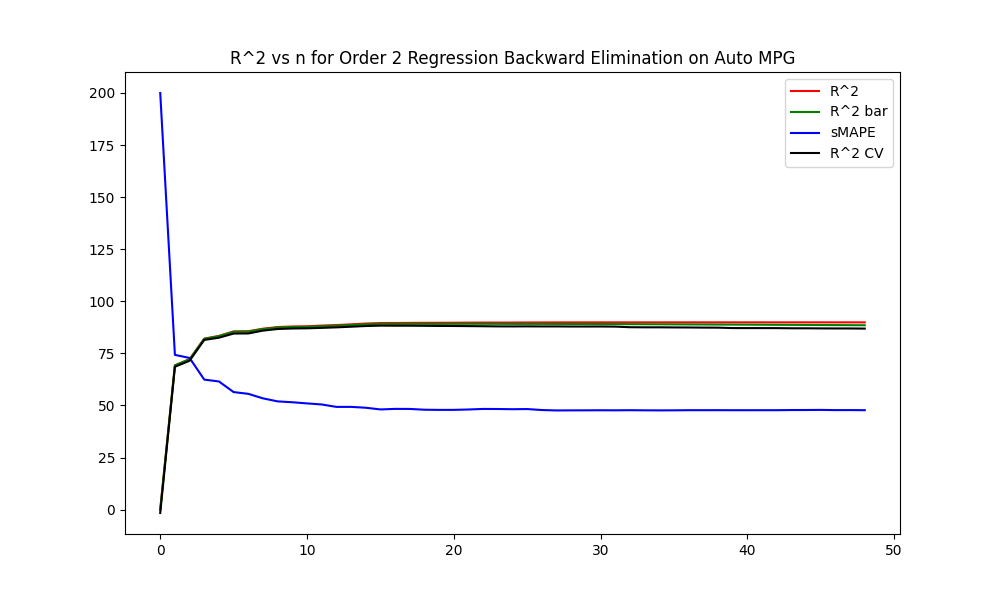
\includegraphics[width=\textwidth]{../Auto_MPG_Statsmodels_Plots/Statsmodels_Order2Reg_rSq_Backward.png}
     \end{subfigure}
     \hfill
     \begin{subfigure}[b]{0.49\textwidth}
         \centering
         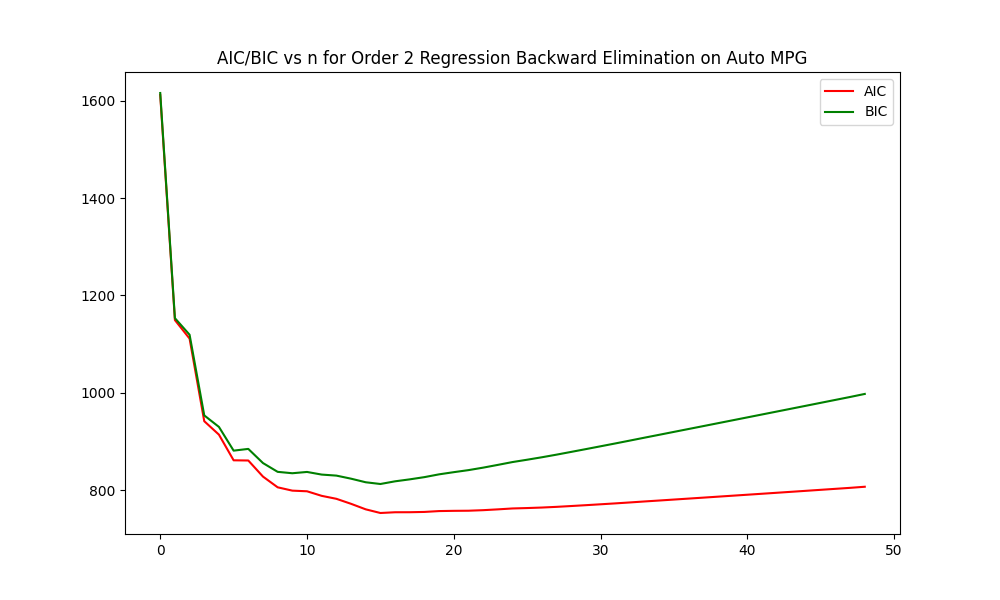
\includegraphics[width=\textwidth]{../Auto_MPG_Statsmodels_Plots/Statsmodels_Order2Reg_AIC_BIC_Backward.png}
     \end{subfigure}
     
     \caption{Auto MPG Order 2 Polynomial Regression Reversed Backward Elimination Quality of Fit Metrics\\ Top Left: Scalation $R^2$, Top Right: Scalation AIC/BIC\\ Bottom Left: Statsmodels $R^2$, Bottom Right: Statsmodels AIC/BIC}
     \label{fig:Auto MPG Order 2 Polynomial Regression Reversed Backward Elimination Quality of Fit Metrics}
\end{figure}

Scalation Stepwise Selection: displacement, horsepower $\times$ acceleration, model year $\times$ model year, weight, weight $\times$ weight, weight $\times$ model year, acceleration, acceleration $\times$ origin 1, model year $\times$ origin 1, acceleration $\times$ acceleration, weight $\times$ acceleration, displacement $\times$ weight, horsepower, horsepower $\times$ model year, model year, origin 1, displacement $\times$ displacement, acceleration $\times$ model year, weight $\times$ origin 1, displacement $\times$ model year, displacement $\times$ origin 1, horsepower $\times$ origin 2, cylinders $\times$ origin 3, weight $\times$ origin 2, displacement $\times$ origin 3, horsepower $\times$ weight, displacement $\times$ horsepower, displacement $\times$ acceleration, acceleration $\times$ origin 3, model year $\times$ origin 2, cylinders $\times$ origin 2, horsepower $\times$ horsepower, horsepower $\times$ origin 3, cylinders $\times$ horsepower, cylinders $\times$ acceleration, cylinders $\times$ model year, origin 2, cylinders $\times$ origin 1, cylinders $\times$ cylinders, cylinders $\times$ weight, origin 3, cylinders, model year $\times$ origin 3, weight $\times$ origin 3, horsepower $\times$ origin 1, displacement $\times$ cylinders, displacement $\times$ origin 2

Statsmodels Stepwise Selection: Null, weight, model year $\times$ model year, weight $\times$ weight, model year, horsepower $\times$ model year, horsepower, acceleration $\times$ origin 1, origin 1, acceleration $\times$ acceleration, model year $\times$ origin 1

\begin{figure}[H]
     \centering
     \captionsetup{justification=centering}
     % First Row
     \begin{subfigure}[b]{0.4\textwidth}
         \centering
         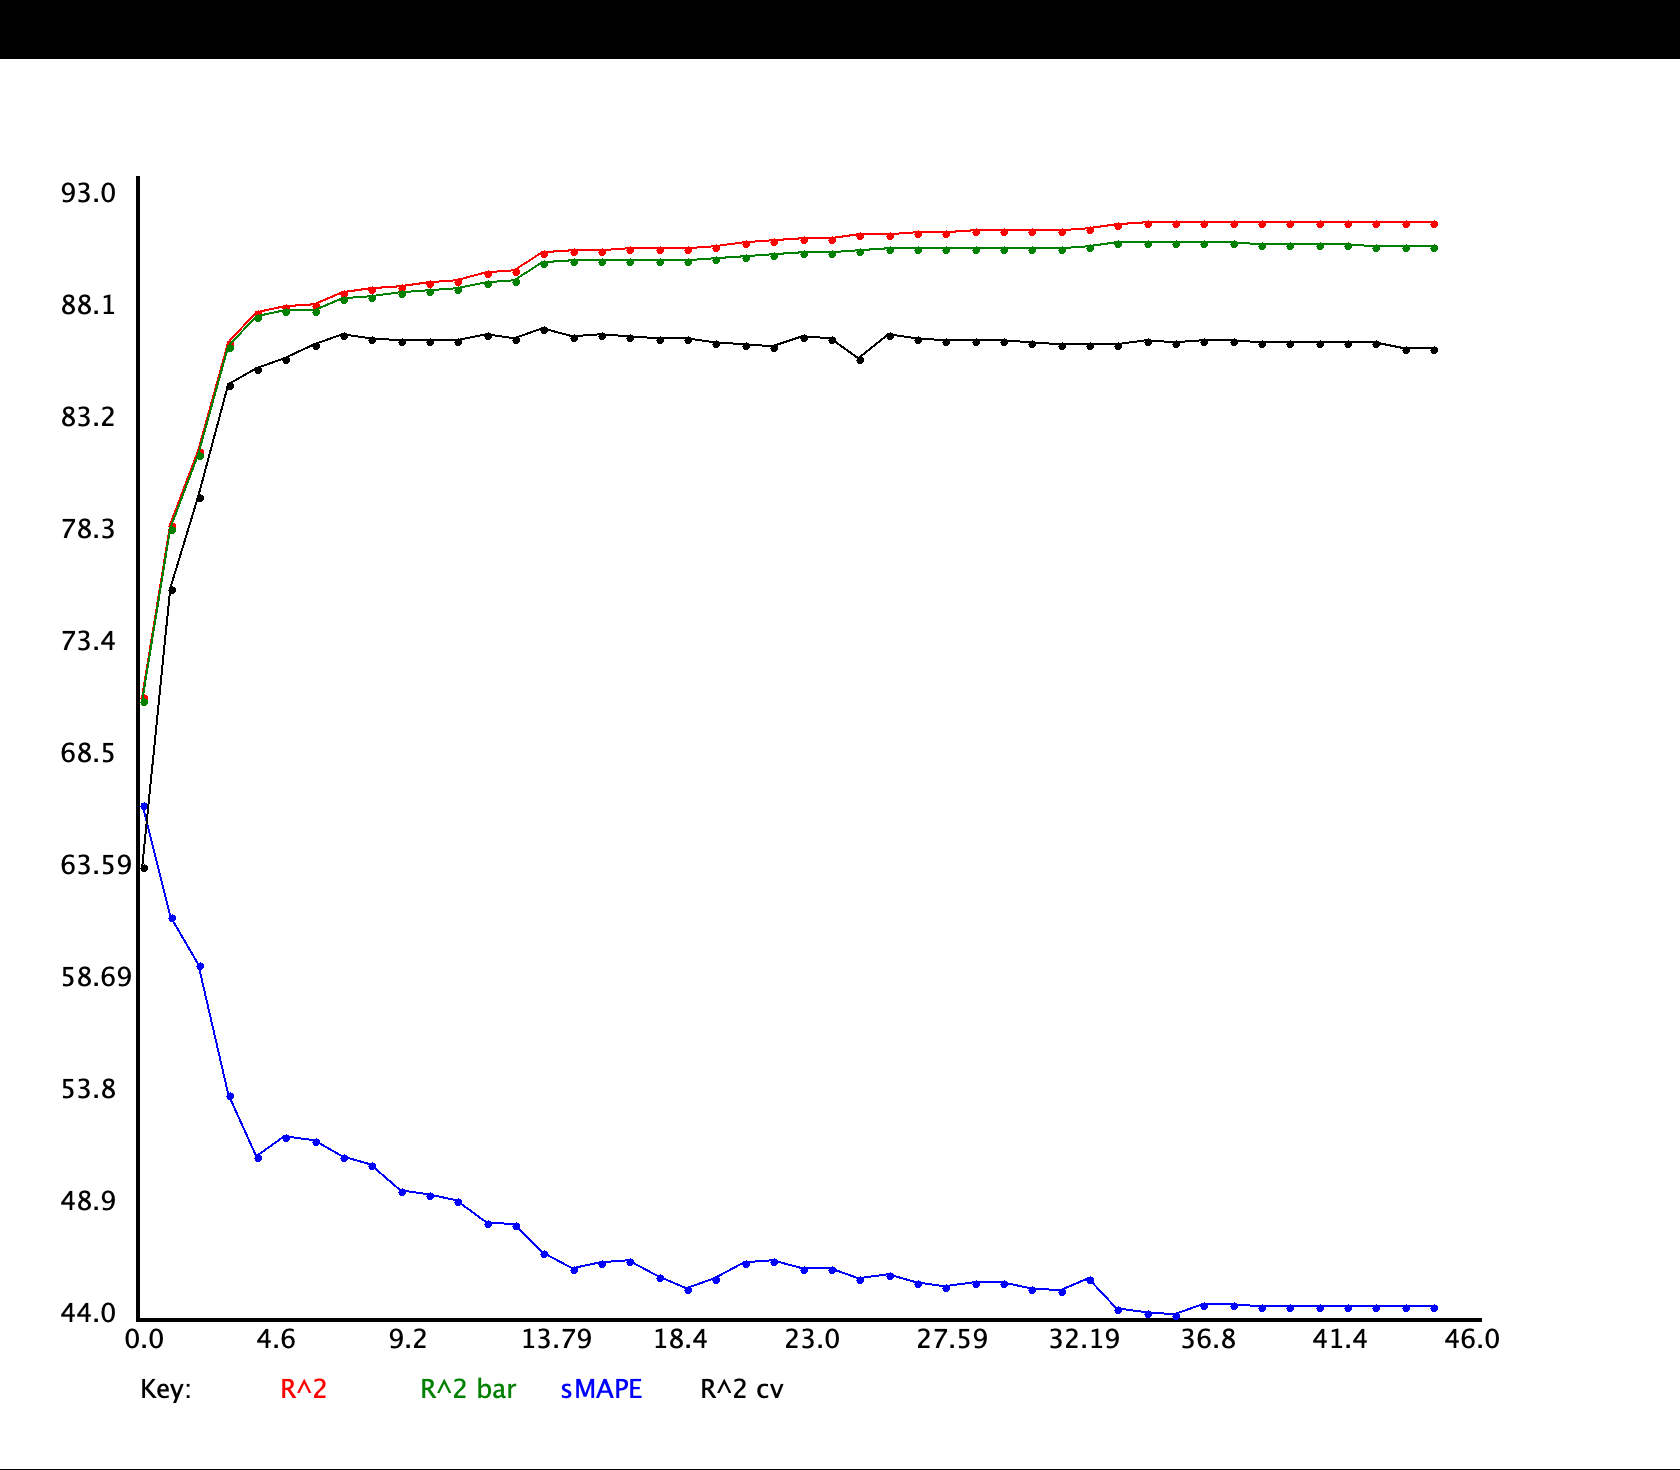
\includegraphics[width=\textwidth]{../Auto_MPG_Scalation_Plots/Scalation_Order2Reg_rSq_Stepwise.png}
     \end{subfigure}
     \hfill
     \begin{subfigure}[b]{0.4\textwidth}
         \centering
         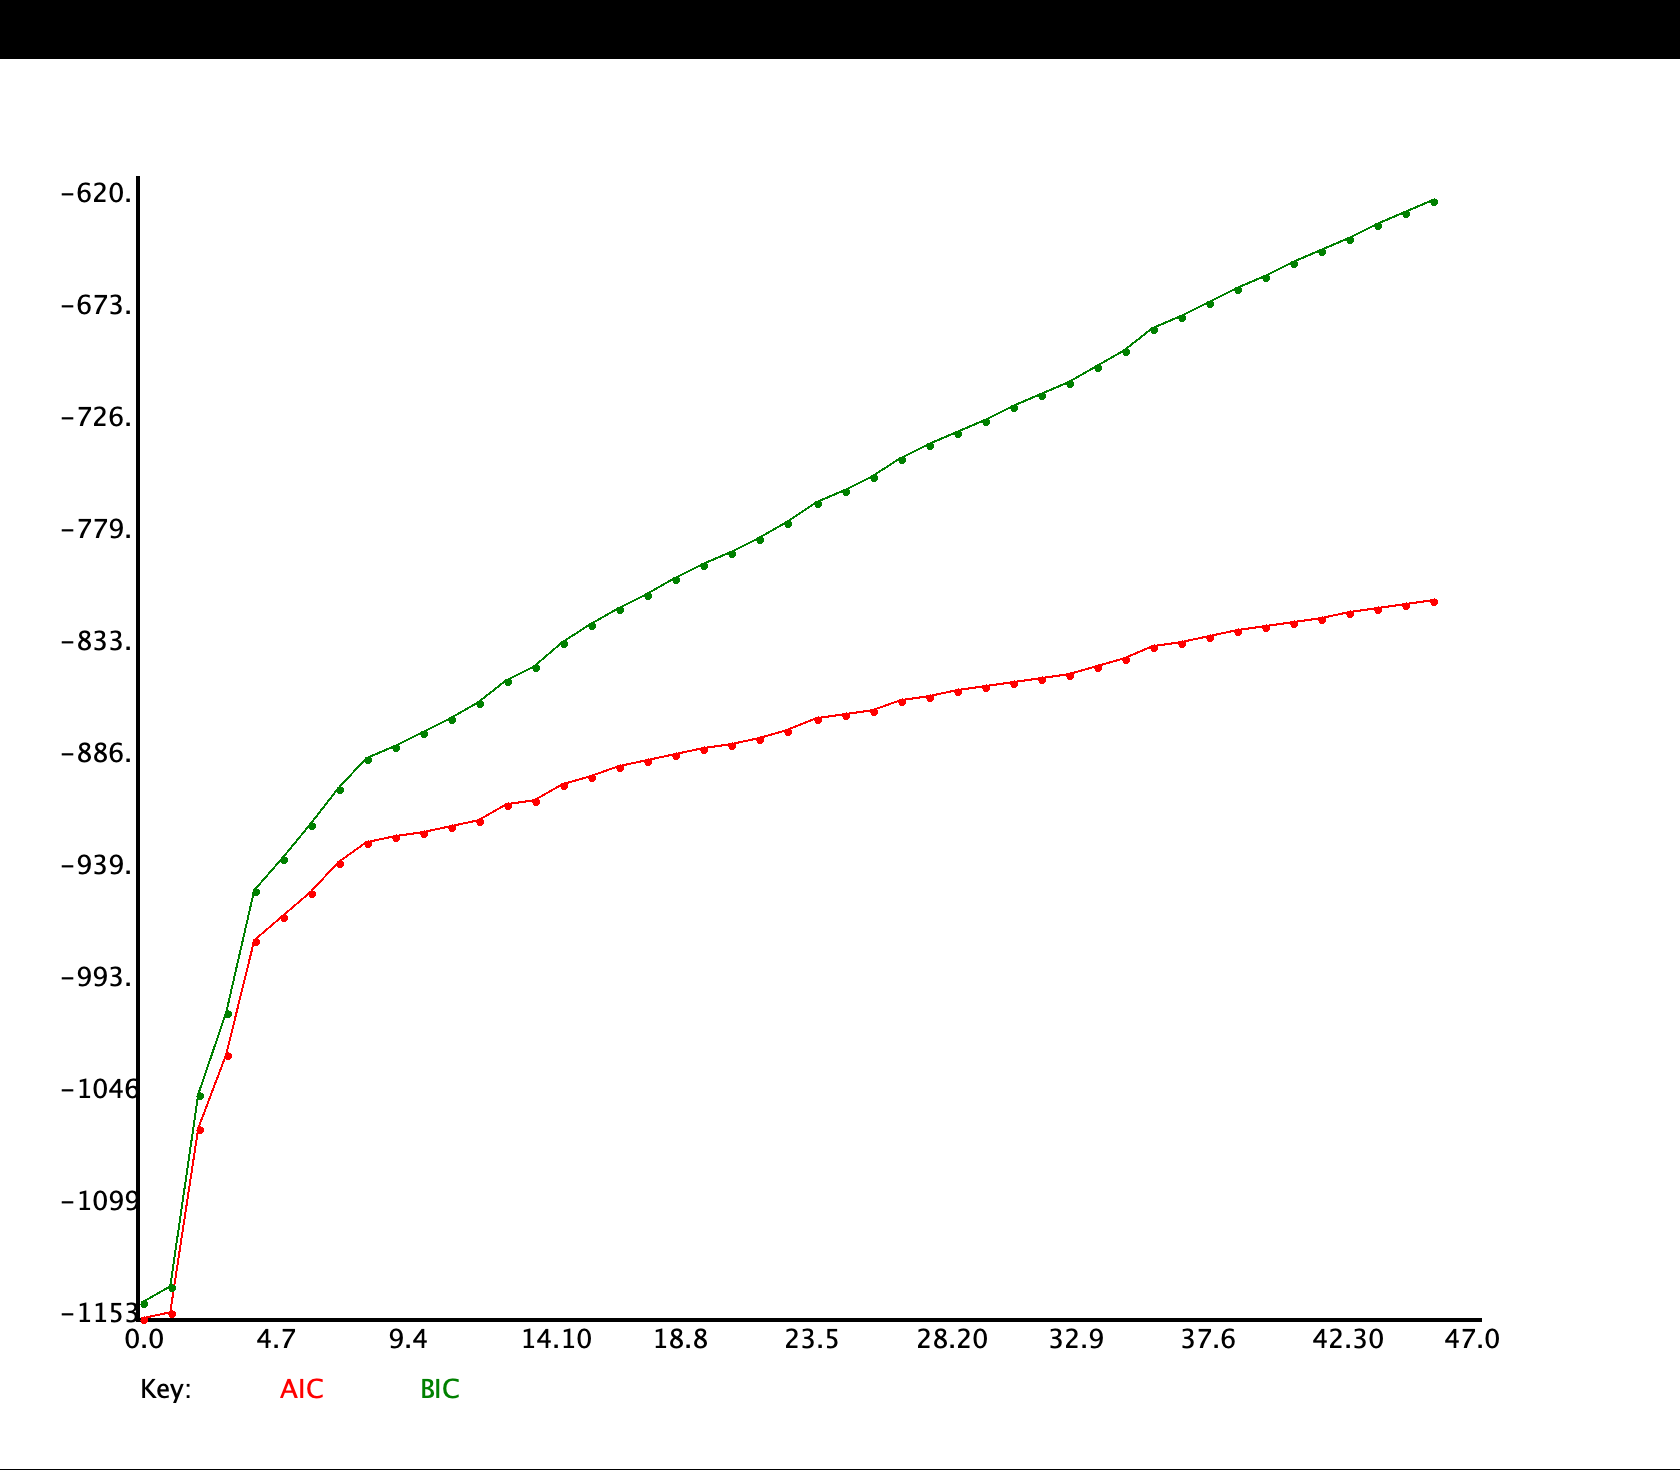
\includegraphics[width=\textwidth]{../Auto_MPG_Scalation_Plots/Scalation_Order2Reg_AIC_BIC_Stepwise.png}
     \end{subfigure}

     \vspace{10pt} % Add some vertical spacing between rows

     % Second Row
     \begin{subfigure}[b]{0.49\textwidth}
         \centering
         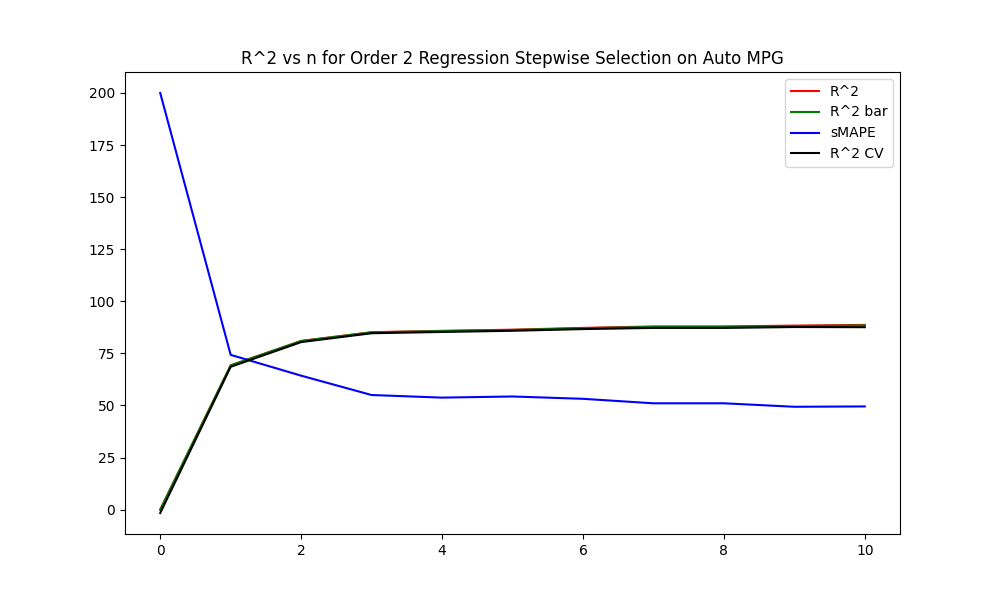
\includegraphics[width=\textwidth]{../Auto_MPG_Statsmodels_Plots/Statsmodels_Order2Reg_rSq_Stepwise.png}
     \end{subfigure}
     \hfill
     \begin{subfigure}[b]{0.49\textwidth}
         \centering
         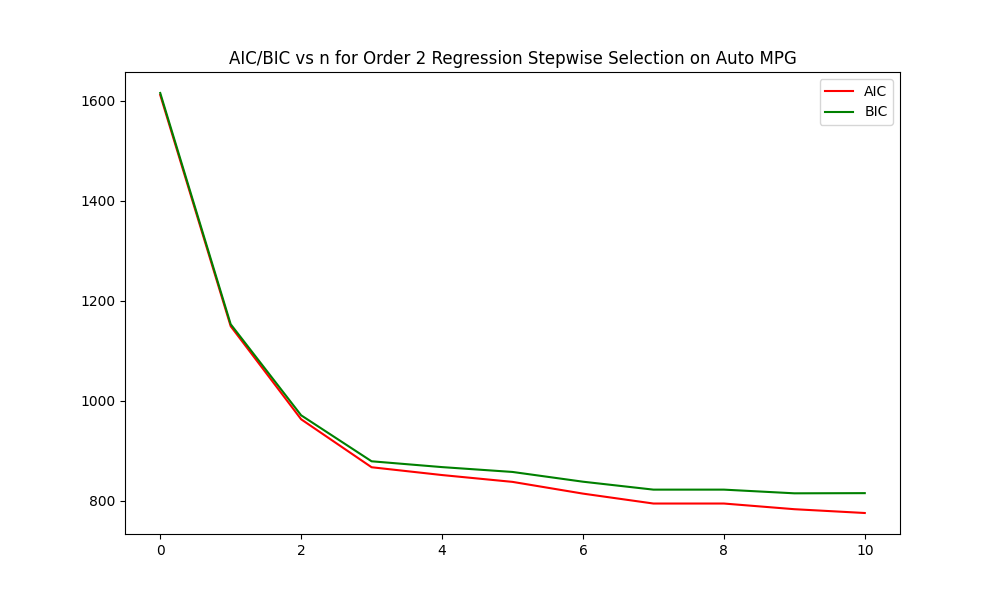
\includegraphics[width=\textwidth]{../Auto_MPG_Statsmodels_Plots/Statsmodels_Order2Reg_AIC_BIC_Stepwise.png}
     \end{subfigure}
     
     \caption{Auto MPG Order 2 Polynomial Regression Stepwise Selection Quality of Fit Metrics\\ Top Left: Scalation $R^2$, Top Right: Scalation AIC/BIC\\ Bottom Left: Statsmodels $R^2$, Bottom Right: Statsmodels AIC/BIC}
     \label{fig:Auto MPG Order 2 Polynomial Regression Stepwise Selection Quality of Fit Metrics}
\end{figure}

\subsection{Model Comparison}

\begin{table}[H]
\centering
\caption{Scalation: - Auto MPG In-Sample QoF Comparison}
\label{tab:Scalation: - Auto MPG In-Sample QoF Comparison}
\begin{tabular}{|c|c|c|c|c|c|c|c|} \hline 
Metric & Regression & Ridge & Lasso & Sqrt & Log1p &  Box-Cox & Order 2 Polynomial \\ \hline \hline 
rSq &0.824199 & 0.808501 &      0.808236 &      0.847208 &      0.859050 &      0.864986 &      0.901459 \\ \hline 
rSqBar &0.820527 &      0.804501 &      0.804741 &      0.844016 &      0.856105 &      0.862166 &      0.887669 \\ \hline 
sst &23819.0 &  23819.0 &       23819.0 &       23819.0 &       23819.0 &       23819.0 &       23819.0 \\ \hline 
sse &4187.39 &  4561.32 &       4567.62 &       3639.36 &       3357.30 &       3215.90 &       2347.15 \\ \hline 
sde &3.27253 &  3.41552 &       3.41612 &       3.04951 &       2.92430 &       2.85675 &       2.45009 \\ \hline 
mse0 &10.6821 & 11.6360 &       11.6521 &       9.28408 &       8.56453 &       8.20383 &       5.98764 \\ \hline 
rmse &3.26835 & 3.41116 &       3.41352 &       3.04698 &       2.92652 &       2.86423 &       2.44696 \\ \hline 
mae &2.50539 &  2.61162 &       2.61088 &       2.25769 &       2.12419 &       2.05497 &       1.74746 \\ \hline 
smape &11.5405 &        64.4083 &       63.9389 &       9.80011 &       9.04308 &       8.67519 &       48.3661 \\ \hline 
m &392.000 &    392.000 &       392.000 &       392.000 &       392.000 &       392.000 &       392.000 \\ \hline 
dfr &8.00000 &  8.00000 &       7.00000 &       8.00000 &       8.00000 &       8.00000 &       48.0000 \\ \hline 
df &383.000 &   383.000 &       384.000 &       383.000 &       383.000 &       383.000 &       343.000 \\ \hline 
fStat &224.451 &        202.126 &       231.209 &       265.459 &       291.783 &       306.717 &       65.3703 \\ \hline 
aic &-1002.46 & -1019.23 &      -1021.50 &      -974.971 &      -959.161 &      -950.732 &      -809.004 \\ \hline 
bic &-966.723 & -983.487 &      -989.729 &      -939.230 &      -923.420 &      -914.990 &      -614.413 \\ \hline 
\end{tabular}
\end{table}

\begin{table}[H]
\centering
\caption{Statsmodels - Auto MPG In-Sample QoF Comparison}
\label{tab:Statsmodels - Auto MPG In-Sample QoF Comparison}
\begin{tabular}{|c|c|c|c|c|c|c|c|}\hline
Metric & Regression & Ridge & Lasso & Sqrt & Log1p & Box-Cox & Order 2 Polynomial \\ \hline \hline
rSq & 0.8242 & 0.8230 & 0.8242 & 0.8584 & 0.8800 & 0.8914 & 0.8990 \\ \hline
rSqBar & 0.8205 & 0.8198 & 0.8210 & 0.8554 & 0.8775 & 0.8891 & 0.8852 \\ \hline
sst & 23818.9935 & 23818.9935 & 23818.9935 & 252.1610 & 41.1728 & 2.1480 & 23818.9935 \\ \hline
sse & 4187.3917 & 4215.8423 & 4187.6288 & 35.7086 & 4.9408 & 0.2334 & 2405.3652 \\ \hline
sde & 3.3065 & 3.3134 & 3.3023 & 0.3053 & 0.1136 & 0.0247 & 2.6443 \\ \hline
mse0 & 10.9331 & 10.7547 & 10.6827 & 0.0932 & 0.0129 & 0.0006 & 6.1361 \\ \hline
rmse & 3.3065 & 3.2794 & 3.2684 & 0.3053 & 0.1136 & 0.0247 & 2.4771 \\ \hline
mae & 2.5054 & 2.4901 & 2.5051 & 2.2577 & 2.1242 & 2.0550 & 1.7742 \\ \hline
smape & 11.5405 & 61.4391 & 62.3436 & 9.8001 & 9.0431 & 8.6752 & 47.7432 \\ \hline
m & 392.0000 & 392.0000 & 392.0000 & 392.0000 & 392.0000 & 392.0000 & 392.0000 \\ \hline
dfr & 8.0000 & 8.0000 & 8.0000 & 8.0000 & 8.0000 & 8.0000 & 48.0000 \\ \hline
df & 383.0000 & 384.0000 & 384.0000 & 383.0000 & 383.0000 & 383.0000 & 344.0000 \\ \hline
fStat & 224.4507 & 223.1941 & 225.0213 & 290.2003 & 351.0758 & 392.8140 & 63.8008 \\ \hline
aic & 2058.9278 & 947.1344 & 944.5022 & 191.2670 & -584.0540 & -1780.7268 & 807.1645 \\ \hline
bic & 2094.6692 & 978.9045 & 976.2723 & 227.0084 & -548.3126 & -1744.9854 & 997.7851 \\ \hline
\end{tabular}
\end{table}

\begin{table}[H]
\centering
\caption{Scalation: - Auto MPG Out-of-Sample QoF Comparison}
\label{tab:Scalation: - Auto MPG Out-of-Sample QoF Comparison}
\begin{tabular}{|c|c|c|c|c|c|c|c|} \hline 
Metric & Regression & Ridge & Lasso & Sqrt & Log1p & Box-Cox & Order 2 Polynomial \\ \hline \hline 
rSq &0.831869 & 0.821456 &      0.824643 &      0.853580 &      0.856892 &      0.852052 &      0.859902 \\ \hline 
rSqBar &0.828357 &      0.817726 &      0.821446 &      0.850521 &      0.853903 &      0.848962 &      0.840296 \\ \hline 
sst &4731.23 &  4731.23 &       4731.23 &       4731.23 &       4731.23 &       4731.23 &       4731.23 \\ \hline 
sse &795.466 &  844.736 &       829.656 &       692.750 &       677.077 &       699.976 &       662.838 \\ \hline 
sde &3.17705 &  3.30307 &       3.27330 &       2.95717 &       2.90754 &       2.93686 &       2.90243 \\ \hline 
mse0 &10.1983 & 10.8299 &       10.6366 &       8.88140 &       8.68048 &       8.97405 &       8.49792 \\ \hline 
rmse &3.19347 & 3.29089 &       3.26138 &       2.98017 &       2.94626 &       2.99567 &       2.91512 \\ \hline 
mae &2.49923 &  2.48838 &       2.45626 &       2.15980 &       2.03303 &       2.02595 &       1.99920 \\ \hline 
smape &12.1086 &        63.9305 &       63.3100 &       9.16865 &       8.33155 &       8.35081 &       50.7296 \\ \hline 
m &78.0000 &    78.0000 &       78.0000 &       78.0000 &       78.0000 &       78.0000 &       78.0000 \\ \hline 
dfr &8.00000 &  8.00000 &       7.00000 &       8.00000 &       8.00000 &       8.00000 &       48.0000 \\ \hline 
df &383.000 &   383.000 &       384.000 &       383.000 &       383.000 &       383.000 &       343.000 \\ \hline 
fStat &236.874 &        220.265 &       257.974 &       279.094 &       286.663 &       275.719 &       43.8600 \\ \hline 
aic &-183.254 & -185.588 &      -186.886 &      -177.868 &      -176.990 &      -178.311 &      -96.1394 \\ \hline 
bic &-162.044 & -164.378 &      -168.032 &      -156.657 &      -155.779 &      -157.101 &      19.3393 \\ \hline 
\end{tabular}
\end{table}

\begin{table}[H]
\centering
\caption{Statsmodels - Auto MPG Out-of-Sample QoF Comparison}
\label{tab:Statsmodels - Auto MPG Out-of-Sample QoF Comparison}
\begin{tabular}{|c|c|c|c|c|c|c|c|}\hline
Metric & Regression & Ridge & Lasso & Sqrt & Log1p & Box-Cox & Order 2 Polynomial \\ \hline \hline
rSq & 0.8388 & 0.8384 & 0.8387 & 0.8630 & 0.8786 & 0.8944 & 0.8913 \\ \hline
rSqBar & 0.8203 & 0.8224 & 0.8228 & 0.8473 & 0.8647 & 0.8823 & 0.7264 \\ \hline
sst & 4910.2699 & 4910.2699 & 4910.2699 & 4910.2699 & 4910.2699 & 4910.2699 & 4910.2699 \\ \hline
sse & 791.7715 & 793.6373 & 791.8769 & 672.9259 & 596.2565 & 518.6048 & 533.9271 \\ \hline
sde & 3.3632 & 3.3434 & 3.3396 & 3.1005 & 2.9186 & 2.7219 & 4.1501 \\ \hline
mse0 & 10.0224 & 10.0460 & 10.0238 & 8.5180 & 7.5476 & 6.5646 & 6.7586 \\ \hline
rmse & 3.1658 & 3.1695 & 3.1660 & 2.9186 & 2.7473 & 2.5622 & 2.5997 \\ \hline
mae & 2.4149 & 2.4065 & 2.4146 & 2.1439 & 2.0120 & 1.9170 & 1.8831 \\ \hline
smape & 11.1538 & 57.5645 & 58.3927 & 9.2958 & 8.6767 & 8.3751 & 47.8555 \\ \hline
m & 79.0000 & 79.0000 & 79.0000 & 79.0000 & 79.0000 & 79.0000 & 79.0000 \\ \hline
dfr & 9.0000 & 8.0000 & 8.0000 & 9.0000 & 9.0000 & 9.0000 & 48.0000 \\ \hline
df & 70.0000 & 71.0000 & 71.0000 & 70.0000 & 70.0000 & 70.0000 & 31.0000 \\ \hline
fStat & 40.4571 & 46.0350 & 46.1571 & 48.9759 & 56.2735 & 65.8640 & 5.2936 \\ \hline
aic & 200.0812 & 198.2671 & 198.0917 & 187.2328 & 177.6766 & 166.6538 & 246.9541 \\ \hline
bic & 221.4062 & 217.2227 & 217.0473 & 208.5578 & 199.0016 & 187.9789 & 360.6876 \\ \hline
\end{tabular}
\end{table}

\begin{table}[H]
\centering
\caption{Scalation - Auto MPG CV Mean Comparison (Averaged over 5 Folds)}
\label{tab:Scalation: - Auto MPG CV Mean Comparison}
\begin{tabular}{|c|c|c|c|c|c|c|c|} \hline
Metric & Regression & Ridge & Lasso & Sqrt & Log1p &  Box-Cox & Order 2 Poly \\\hline \hline
rSq & 0.808 & 0.797 & 0.801 & 0.835 & 0.849 & 0.856 & 0.865 \\\hline
rSqBar & 0.804 & 0.793 & 0.797 & 0.831 & 0.845 & 0.853 & 0.846 \\\hline
sst & 4700.481 & 4700.481 & 4700.481 & 4700.481 & 4700.481 & 4700.481 & 4700.481 \\\hline
sse & 898.143 & 955.120 & 936.371 & 777.312 & 713.304 & 679.185 & 628.878 \\\hline
sde & 3.326 & 3.439 & 3.419 & 3.101 & 2.976 & 2.908 & 2.823 \\\hline
mse0 & 11.515 & 12.245 & 12.005 & 9.966 & 9.145 & 8.708 & 8.063 \\\hline
rmse & 3.388 & 3.491 & 3.456 & 3.149 & 3.015 & 2.936 & 2.835 \\\hline
mae & 2.585 & 2.681 & 2.651 & 2.320 & 2.181 & 2.111 & 2.038 \\\hline
smape & 11.891 & 66.453 & 65.555 & 10.048 & 9.273 & 8.898 & 52.629 \\\hline
m & 78.000 & 78.000 & 78.000 & 78.000 & 78.000 & 78.000 & 78.000 \\\hline
dfr & 8.000 & 8.000 & 7.000 & 8.000 & 8.000 & 8.000 & 48.000 \\\hline
df & 383.000 & 383.000 & 384.000 & 383.000 & 383.000 & 383.000 & 343.000 \\\hline
fStat & 203.481 & 188.950 & 222.193 & 243.316 & 270.208 & 290.795 & 46.760 \\\hline
aic & -188.407 & -190.712 & -191.930 & -182.765 & -179.160 & -177.090 & -94.098 \\\hline
bic & -167.196 & -169.502 & -173.076 & -161.555 & -157.950 & -155.880 & 21.381 \\\hline
\end{tabular}
\end{table}

\begin{table}[H]
\centering
\caption{Statsmodels - Auto MPG CV Mean Comparison (Averaged over 5 Folds)}
\label{tab:Statsmodels - Auto MPG CV Mean Comparison}
\begin{tabular}{|c|c|c|c|c|c|c|c|}\hline
Metric & Regression & Ridge & Lasso & Sqrt & Log1p & Box-Cox & Order 2 Poly \\\hline \hline
rSq & 0.8062 & 0.8101 & 0.8103 & 0.8327 & 0.8462 & 0.8531 & 0.8691 \\\hline
rSqBar & 0.7839 & 0.7912 & 0.7915 & 0.8134 & 0.8285 & 0.8362 & 0.6666 \\\hline
sst & 4721.1782 & 4721.1782 & 4721.1782 & 4721.1782 & 4721.1782 & 4721.1782 & 4721.1782 \\\hline
sse & 895.0561 & 881.2419 & 878.1148 & 773.6072 & 711.7754 & 679.6400 & 607.1392 \\\hline
sde & 3.5846 & 3.5349 & 3.5274 & 3.3326 & 3.1961 & 3.1201 & 4.4435 \\\hline
mse0 & 11.4215 & 11.2436 & 11.2044 & 9.8710 & 9.0822 & 8.6735 & 7.7447 \\\hline
rmse & 3.3725 & 3.3497 & 3.3426 & 3.1355 & 3.0070 & 2.9355 & 2.7667 \\\hline
mae & 2.5894 & 2.5567 & 2.5643 & 2.3318 & 2.1900 & 2.1170 & 1.9847 \\\hline
smape & 11.9879 & 62.6259 & 63.2520 & 10.1388 & 9.3196 & 8.9379 & 52.2568 \\\hline
m & 78.4000 & 78.4000 & 78.4000 & 78.4000 & 78.4000 & 78.4000 & 78.4000 \\\hline
dfr & 9.0000 & 8.0000 & 8.0000 & 9.0000 & 9.0000 & 9.0000 & 48.0000 \\\hline
df & 69.4000 & 70.4000 & 70.4000 & 69.4000 & 69.4000 & 69.4000 & 30.4000 \\\hline
fStat & 33.9820 & 39.0075 & 39.3824 & 40.5073 & 44.7718 & 47.7890 & 4.5978 \\\hline
aic & 208.2629 & 205.3684 & 204.9728 & 196.8483 & 190.2479 & 186.2788 & 254.6013 \\\hline
bic & 229.5191 & 224.2628 & 223.8672 & 218.1045 & 211.5042 & 207.5350 & 367.9679 \\\hline
\end{tabular}
\end{table}

\section{California Housing Prices}\label{House Prices}

\subsection{Exploratory Data Analysis}

The California Housing Prices dataset contains $20640$ observations each having $10$ variables. These variables are:
\begin{itemize}
	\item longitude: A measure of how far west a house is; a higher value is farther west.
	\item latitude: A measure of how far north a house is; a higher value is farther north.
	\item housing median age: Median age of a house within a block; a lower number is a newer building.
	\item total rooms: Total number of rooms within a block.
	\item total bedrooms: Total number of bedrooms within a block.
	\item population: Total number of people residing within a block.
	\item households: Total number of households, a group of people residing within a home unit, for a block.
	\item median income: Median income for households within a block of houses (measured in tens of thousands of US Dollars).
	\item ocean proximity: Location of the house w.r.t ocean/sea
	\item median house value: (The target variable) Median house value for households within a block (measured in US Dollars)
\end{itemize}

The total bedrooms feature contains $207$ missing values, representing approximately $1\%$ of the dataset. Because all other features are fully populated, these rows were excluded from the analysis. For modeling purposes, we appended an intercept column of ones and converted the categorical ocean proximity variable into dummy variables (ocean\_proximity\_INLAND, ocean\_proximity\_ISLAND, ocean\_proximity\_NEAR BAY, ocean\_proximity\_NEAR OCEAN), omitting ocean\_proximity\_$<$1H OCEAN to prevent multi-collinearity.

Univariate distributions are visualized in \Cref{fig:House Prices Histograms} (histograms/count-plots) and \Cref{fig:House Prices Box Plots} (box plots for continuous variables). The visualizations reveal that the distributions of longitude, latitude, and housing median age are bimodal shaped, whereas total rooms, total bedrooms, population, households, median income, and median house value all right-skewed; while they resemble normal distributions, they are heavily truncated on the left and feature long right tails. Notably, all of total rooms, total bedrooms, population, households, median income, and median house value contain many outliers, some being very extreme. Finally, ocean proximity $<$H OCEAN is the most prevalent, followed by INLAND. Ocean proximity NEAR BAY and NEAR OCEAN show similar levels of representation, while ISLAND has very little representation.

\begin{figure}[H]
    \centering
    \captionsetup{justification=centering}
    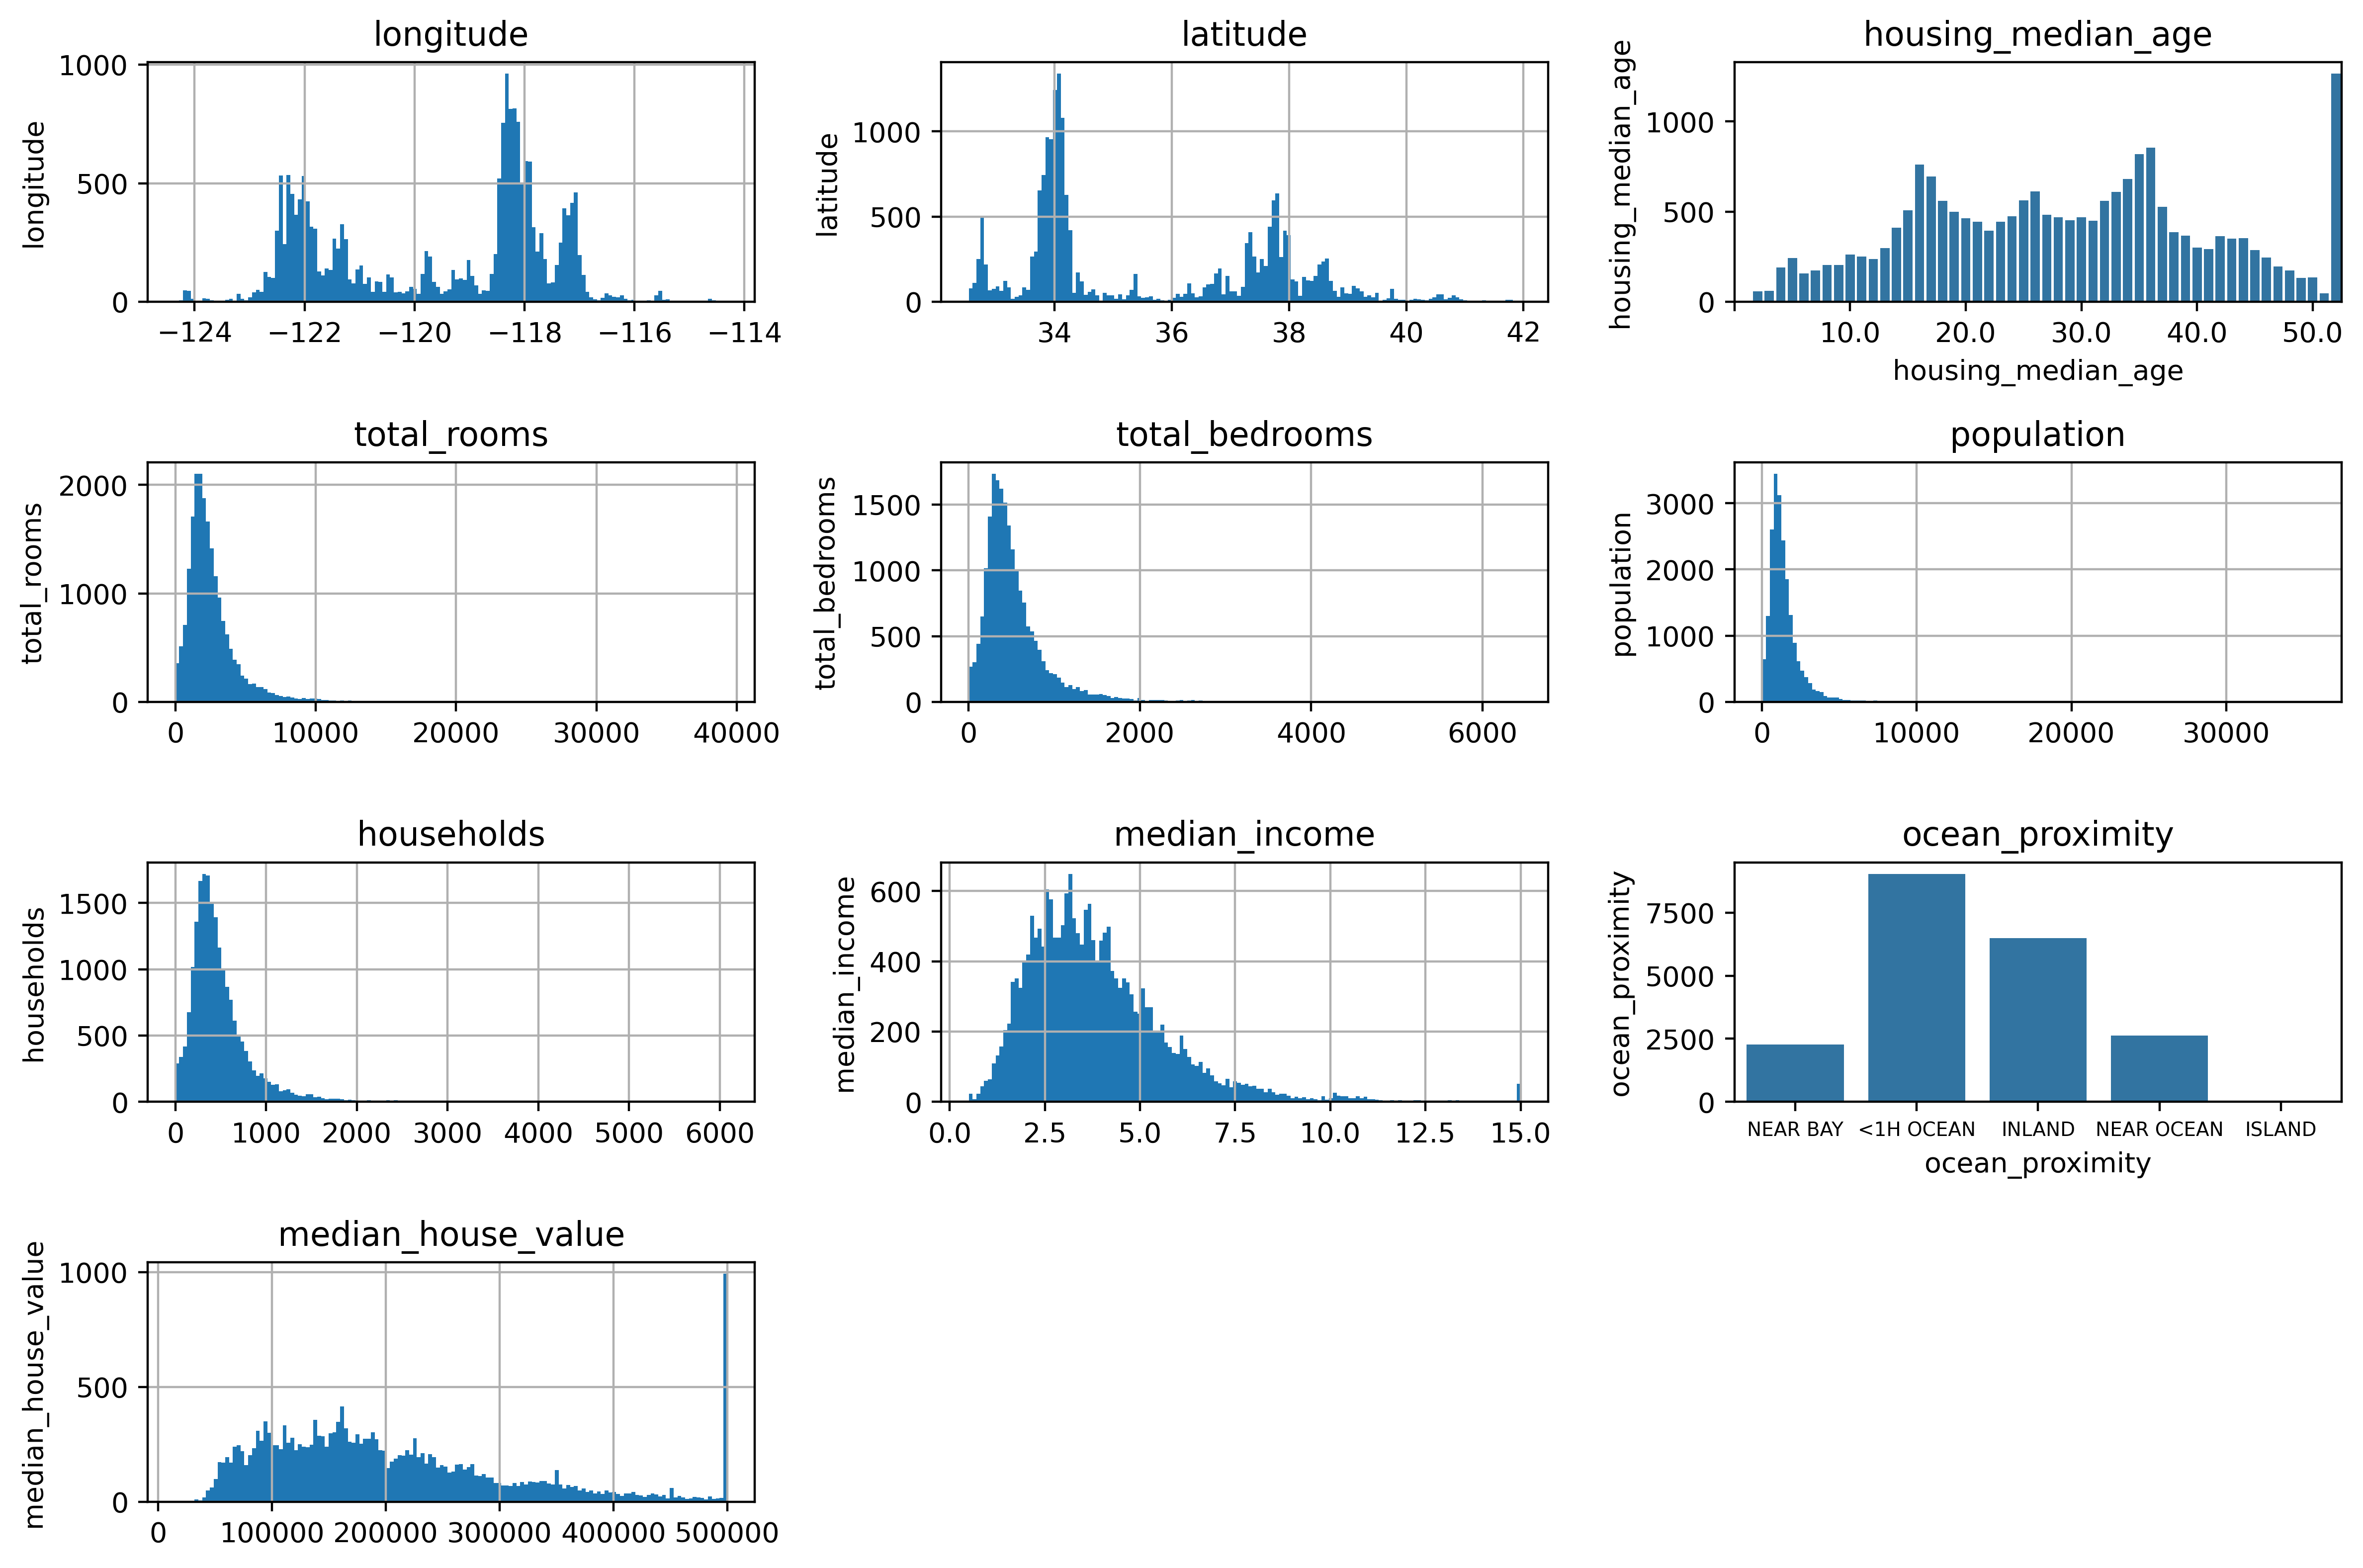
\includegraphics[width=0.75\textwidth]{../House_Prices/histograms.png} 
    \caption{California House Prices Histograms and Count-Plots}
    \label{fig:House Prices Histograms}
\end{figure}

\begin{figure}[H]
    \centering
    \captionsetup{justification=centering}
    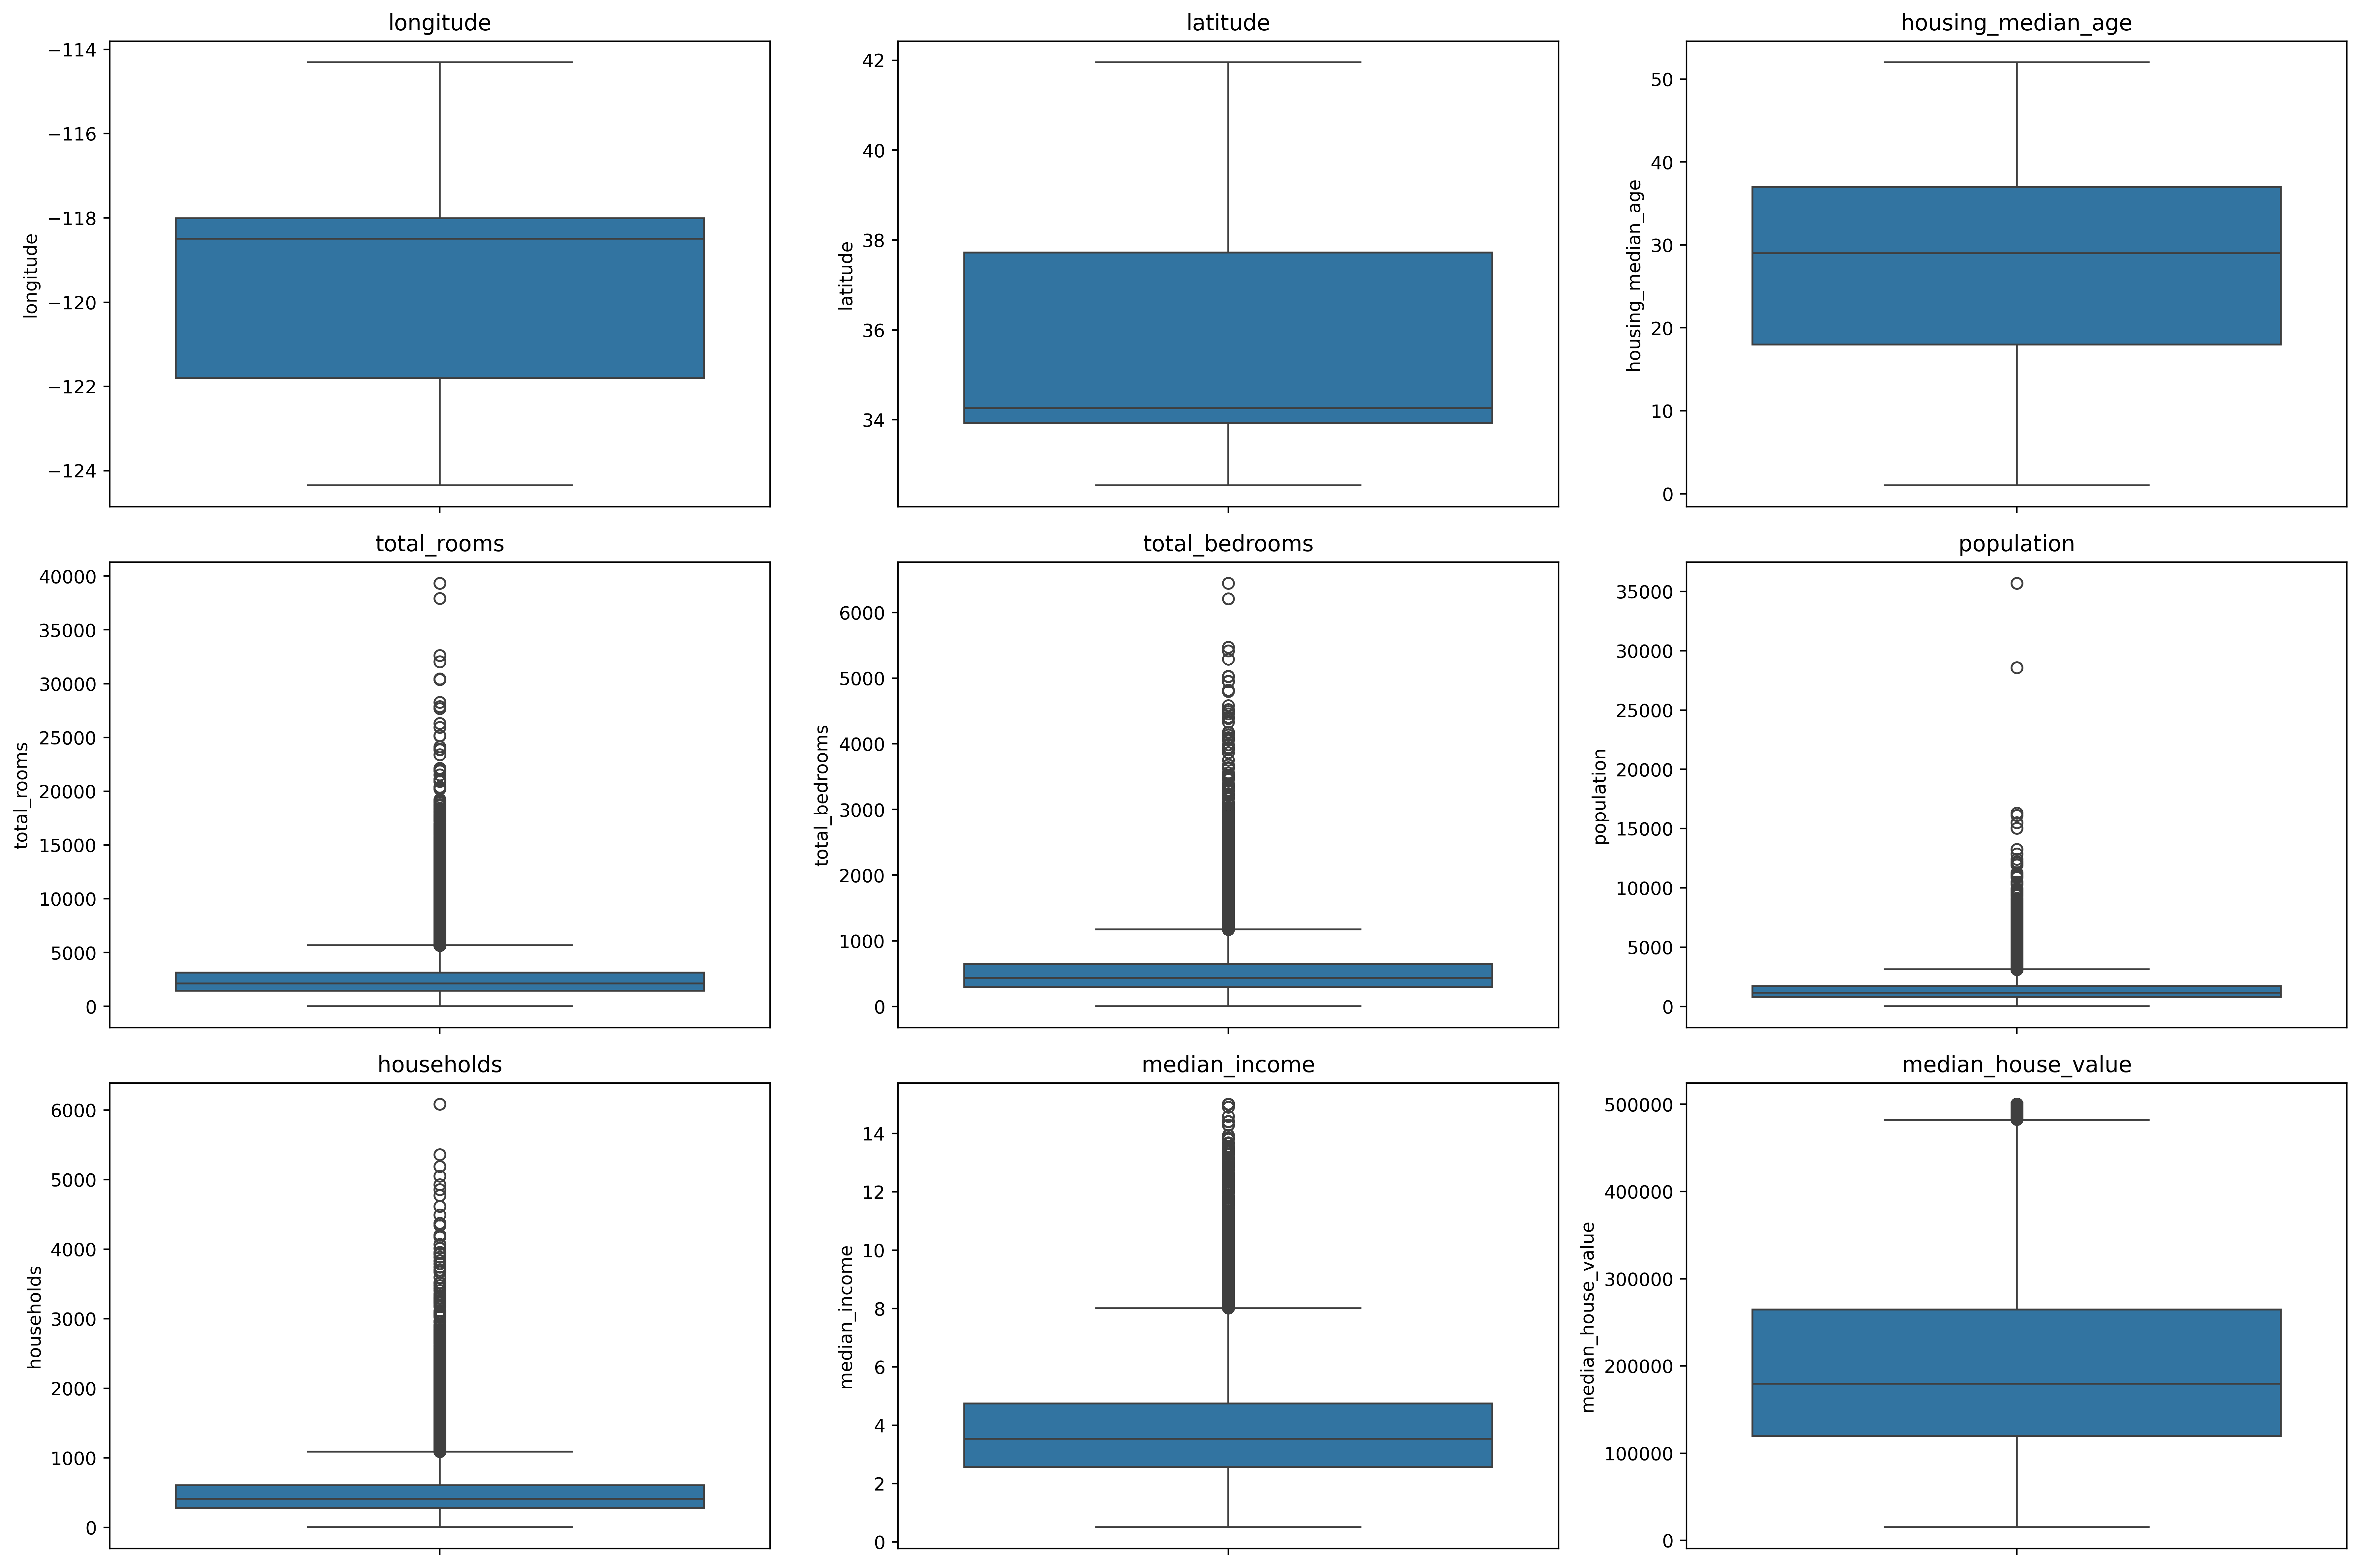
\includegraphics[width=0.75\textwidth]{../House_Prices/boxplots.png} 
    \caption{California House Prices Box Plots}
    \label{fig:House Prices Box Plots}
\end{figure}

\Cref{fig:House Prices Scatterplots} displays the bivariate relationships between each predictor and the target variable, median house value, while the corresponding correlation matrix is provided in \Cref{fig:House Prices Correlation Heat Map}. Analysis of these figures indicates that median income has the strongest correlation with median house value. Furthermore, the figures reveal that the remaining predictor variables exhibit no discernible relationship with median house value, appearing as randomly distributed clusters with no clear linear or non-linear patterns. Last, there is significant inter-correlations between several variables; longitude and latitude; and total rooms, total bedrooms, population, and households; suggesting potential multi-collinearity.

\begin{figure}[H]
    \centering
    \captionsetup{justification=centering}
    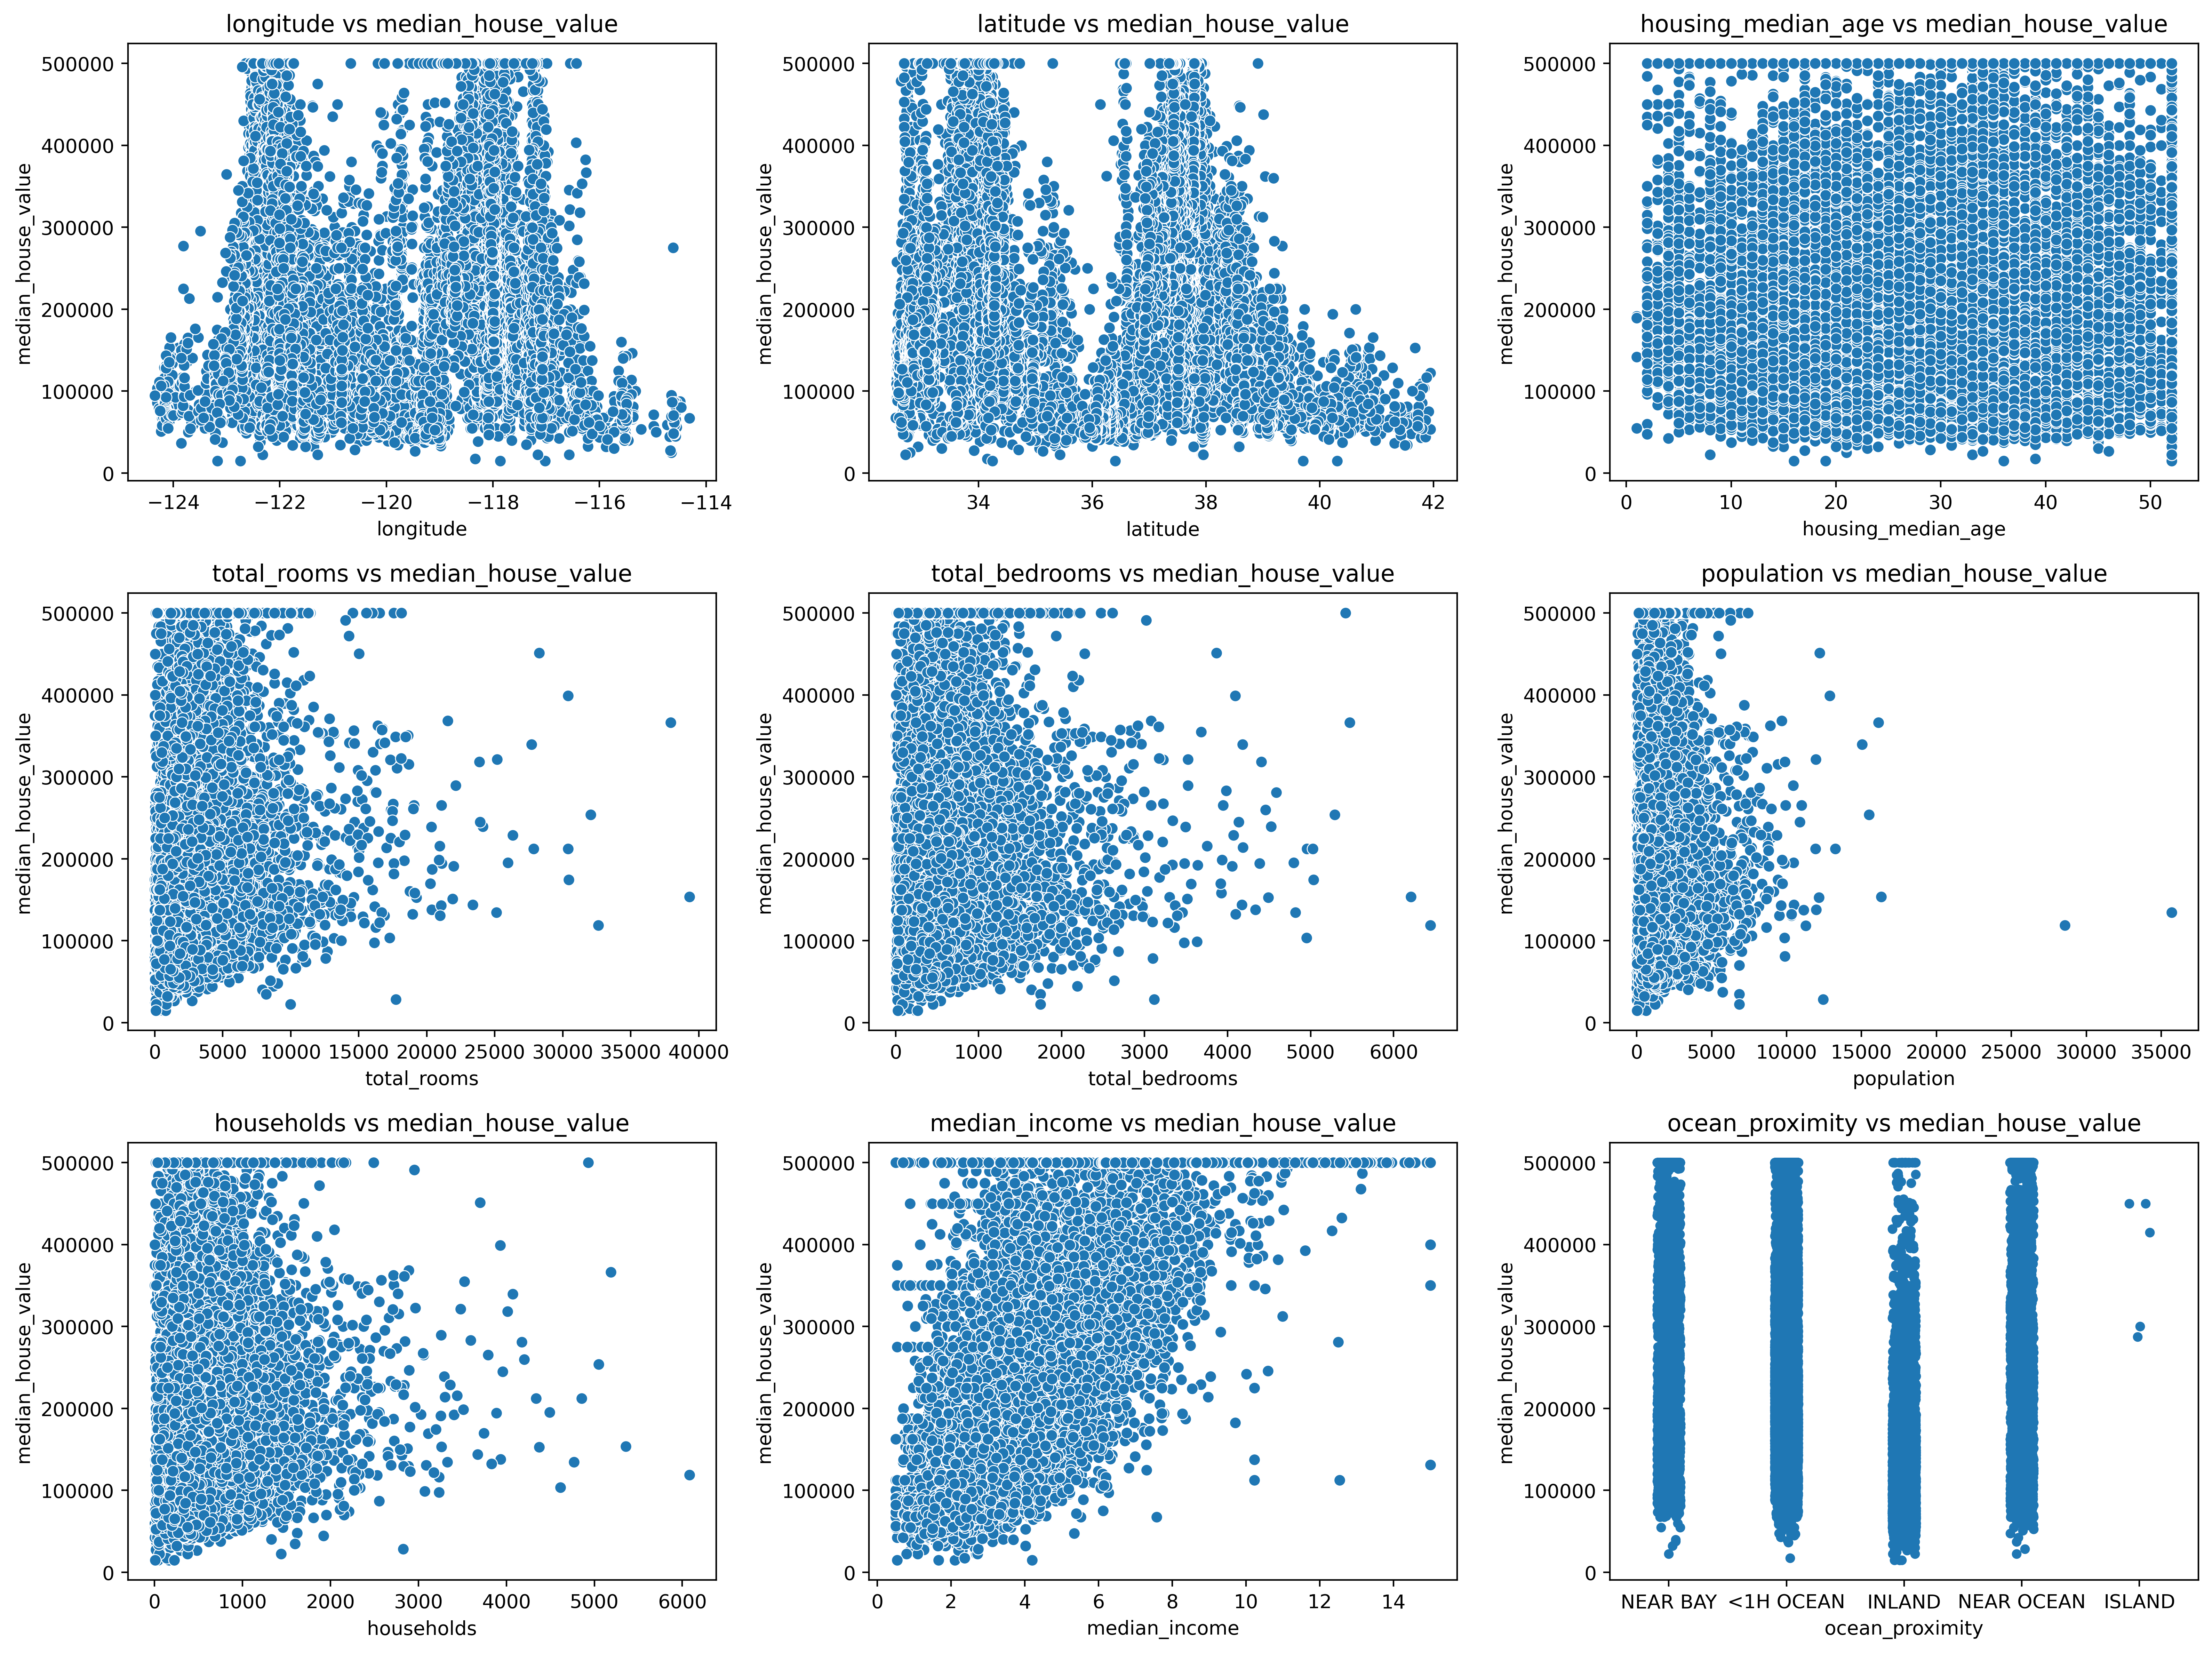
\includegraphics[width=0.75\textwidth]{../House_Prices/scatterplots.png} 
    \caption{California House Prices Scatterplots}
    \label{fig:House Prices Scatterplots}
\end{figure}

\begin{figure}[H]
    \centering
    \captionsetup{justification=centering}
    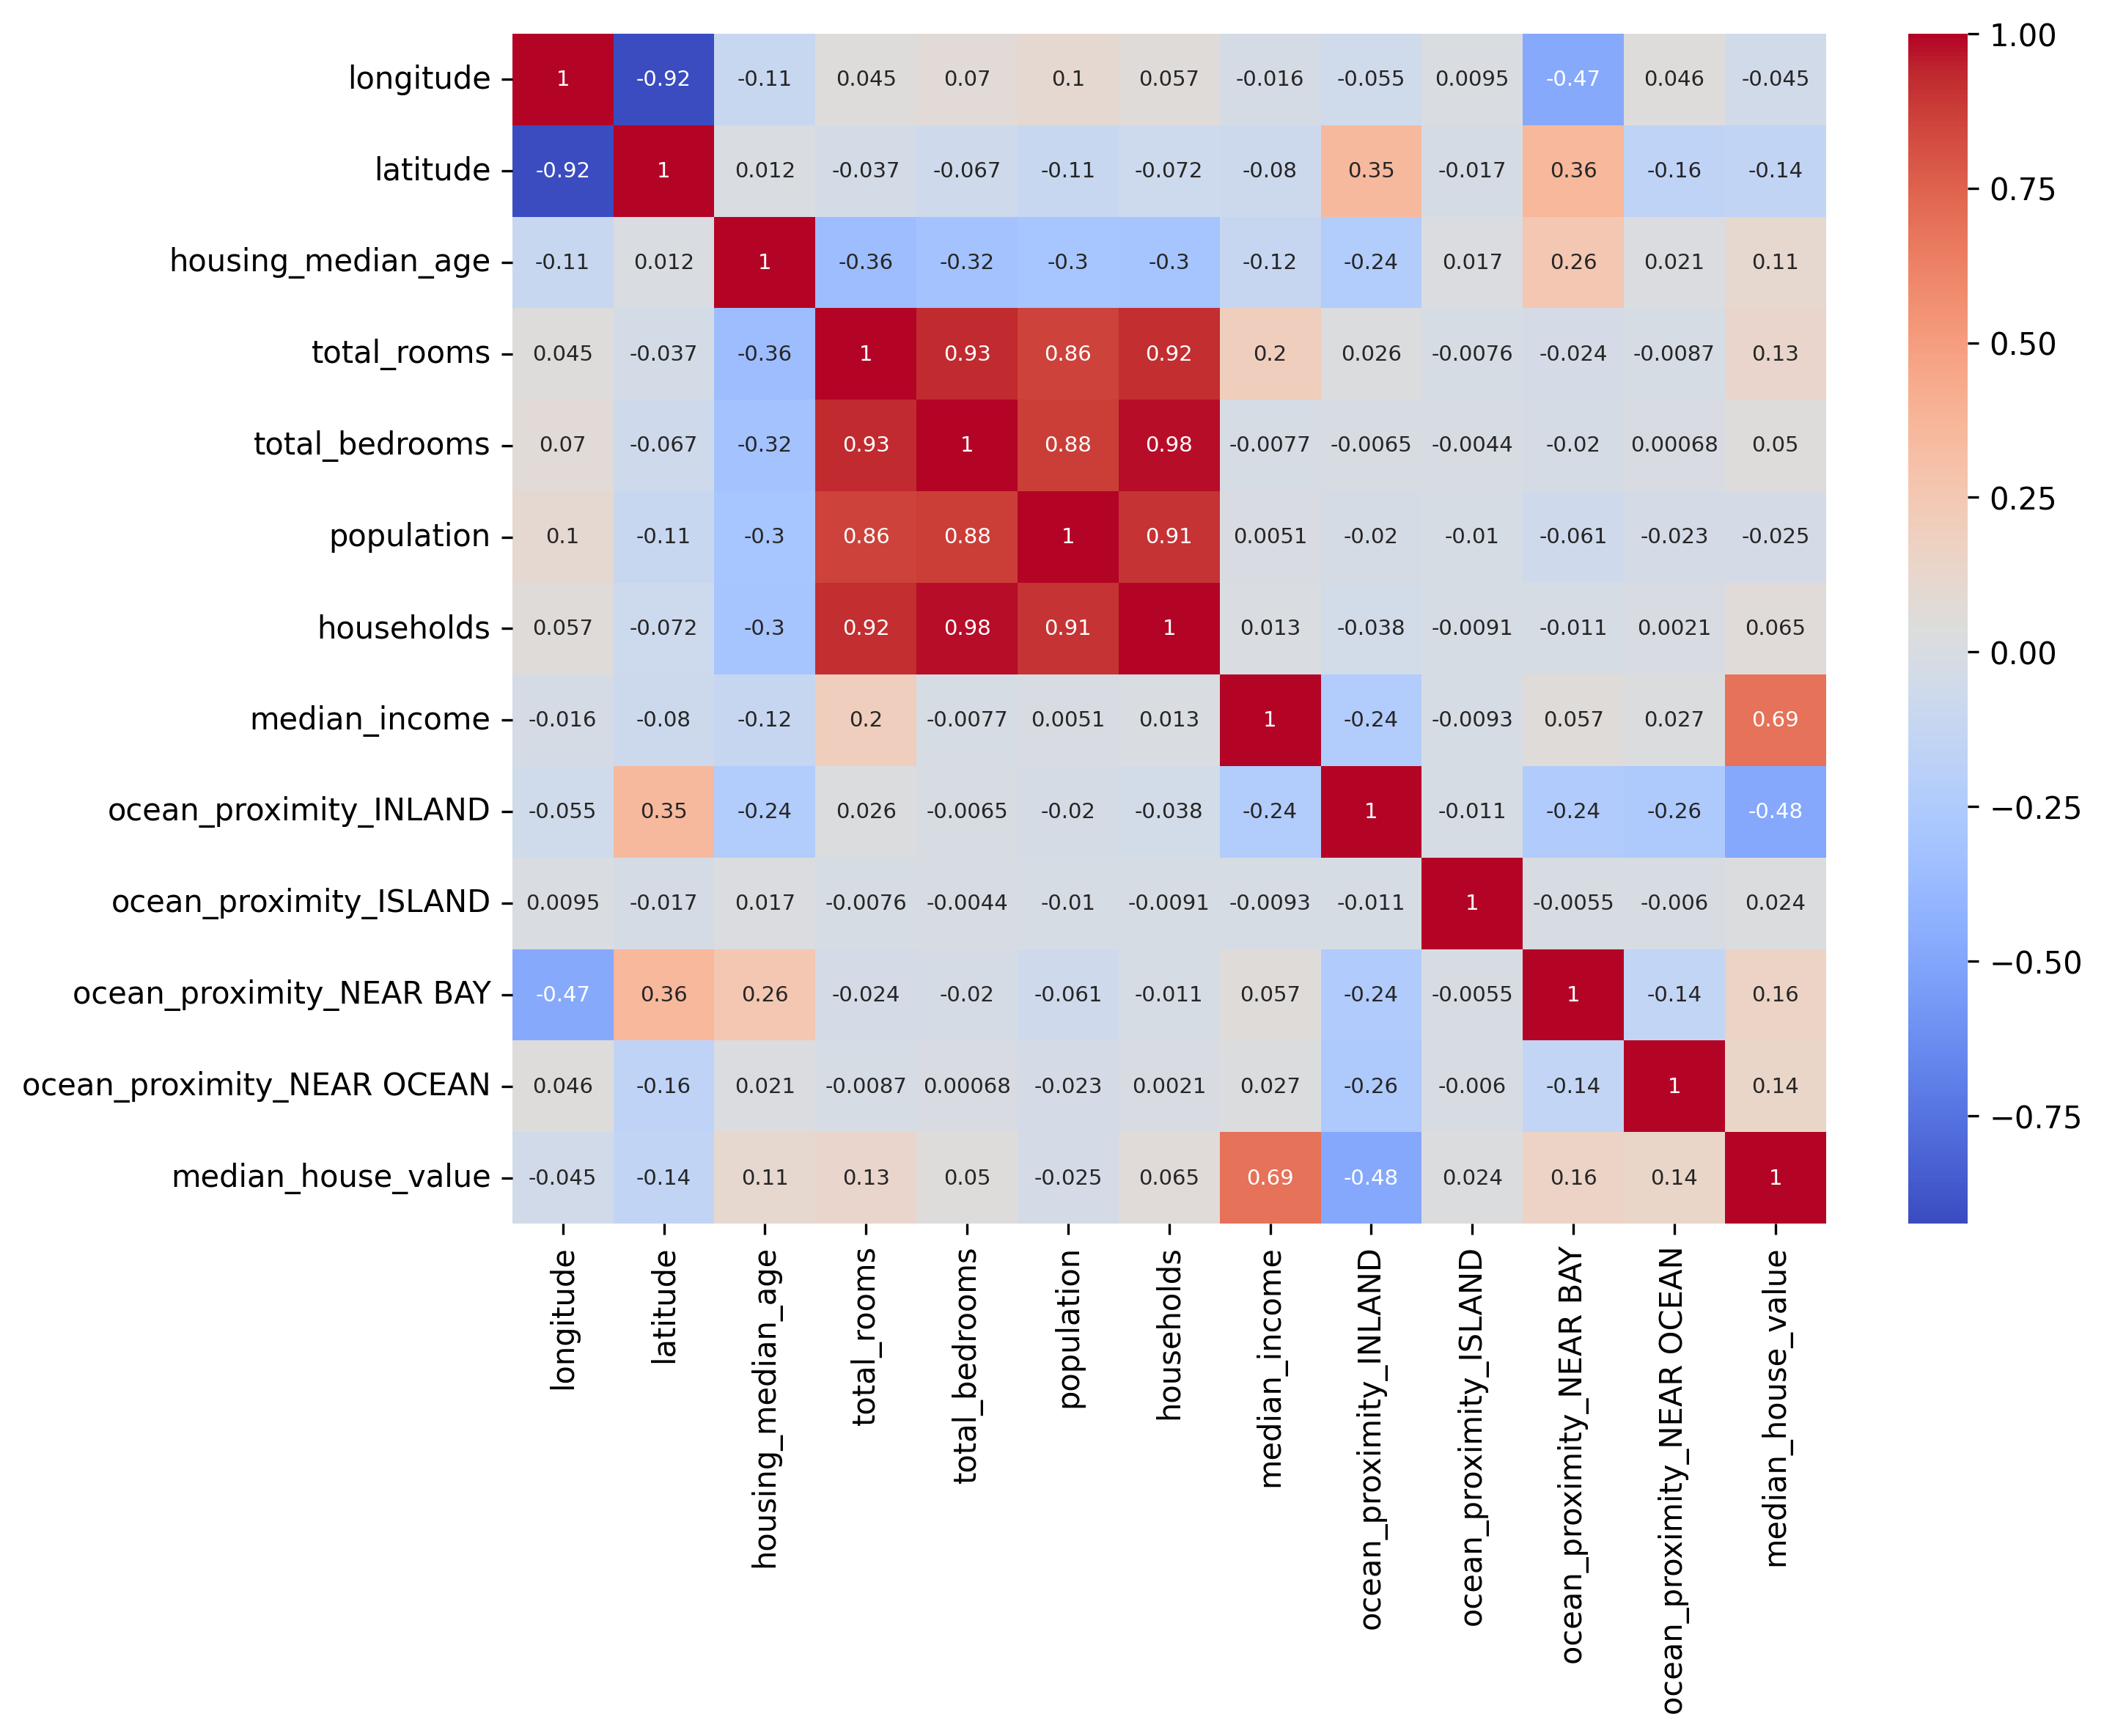
\includegraphics[width=0.5\textwidth]{../House_Prices/correlation_heatmap.png} 
    \caption{California House Prices Correlation Heat Map}
    \label{fig:House Prices Correlation Heat Map}
\end{figure}

\Cref{fig:House Prices Hue Plots} illustrates the bivariate relationships among the predictor variables, with data points colored by the target variable, median house value. These visualizations further substantiate the high degree of correlation observed between; longitude and latitude; and total rooms, total bedrooms, population, and households. Furthermore, the general lack of structured patterns across these plots suggests that the inclusion of interaction terms may not improve model performance.

\begin{figure}[H]
    \centering
    \captionsetup{justification=centering}
    \includegraphics[width=0.9\textwidth]{../House_Prices/Hue_Plots.png} 
    \caption{California House Prices Hue Plots}
    \label{fig:House Prices Hue Plots}
\end{figure}

\subsection{Multiple Linear Regression}

\subsubsection{Quality of Fit}

\begin{table}[H]
\centering
\caption{Scalation - California House Prices Linear Regression}
\label{tab:Scalation - House Prices Linear Regression}
\begin{tabular}{|c|c|c|} \hline 
Metric & In-Sample & 80-20 Split \\ \hline \hline 
rSq &0.646464 & 0.643048 \\ \hline 
rSqBar &0.646256 &      0.642838 \\ \hline 
sst &2.72264e+14 &      5.31945e+13 \\ \hline 
sse &9.62553e+13 &      1.89879e+13 \\ \hline 
sde &68636.8 &  68138.4 \\ \hline 
mse0 &4.71078e+09 &     4.64706e+09 \\ \hline 
rmse &68635.1 & 68169.4 \\ \hline 
mae &49748.2 &  49532.1 \\ \hline 
smape &26.2930 &        26.4602 \\ \hline 
m &20433.0 &    4086.00 \\ \hline 
dfr &12.0000 &  12.0000 \\ \hline 
df &20420.0 &   20420.0 \\ \hline 
fStat &3111.61 &        3065.54 \\ \hline 
aic &-256520 &  -51247.9 \\ \hline 
bic &-256417 &  -51165.8 \\ \hline 
\end{tabular}
\end{table}

\begin{table}[H]
\centering
\caption{Statsmodels - California House Prices Linear Regression}
\label{tab:Statsmodels - House Prices Linear Regression}
\begin{tabular}{|c|c|c|}\hline
Metric & In-Sample & 80-20 Split \\ \hline \hline
rSq & 0.6465 & 0.6526 \\ \hline
rSqBar & 0.6463 & 0.6516 \\ \hline
sst & 272264434648930.1562 & 54723646809444.8438 \\ \hline
sse & 96255324900327.4375 & 19010465918035.0938 \\ \hline
sde & 68656.9511 & 68310.2490 \\ \hline
mse0 & 4713776929.4969 & 4651447496.4608 \\ \hline
rmse & 68656.9511 & 68201.5212 \\ \hline
mae & 49748.1895 & 49964.0128 \\ \hline
smape & 26.2930 & 26.2959 \\ \hline
m & 20433.0000 & 4087.0000 \\ \hline
dfr & 12.0000 & 13.0000 \\ \hline
df & 20420.0000 & 4074.0000 \\ \hline
fStat & 3111.6080 & 588.7263 \\ \hline
aic & 513118.9804 & 91004.4358 \\ \hline
bic & 513222.0042 & 91086.5382 \\ \hline
\end{tabular}
\end{table}

\begin{table}[H]
\centering
\caption{Scalation - California House Prices Linear Regression CV}
\label{tab:Scalation - California House Prices Linear Regression CV}
\begin{tabular}{|c|c|c|c|c|c|}\hline
Metric & num folds & min & max & mean & stdev \\ \hline \hline
rSq & 5 & 0.628 & 0.661 & 0.645 & 0.012 \\ \hline
rSqBar & 5 & 0.628 & 0.661 & 0.645 & 0.012 \\ \hline
sst & 5 & 53194492241132.980 & 57310203956796.625 & 54411355017051.000 & 1675890609056.710 \\ \hline
sse & 5 & 18091271374124.617 & 21300107623723.953 & 19326273860287.414 & 1203800943358.952 \\ \hline
sde & 5 & 66545.500 & 72143.458 & 68734.562 & 2094.101 \\ \hline
mse0 & 5 & 4427623929.056 & 5212948512.904 & 4729876128.313 & 294615992.011 \\ \hline
rmse & 5 & 66540.393 & 72200.751 & 68748.019 & 2117.175 \\ \hline
mae & 5 & 48559.672 & 51928.415 & 49805.806 & 1284.904 \\ \hline
smape & 5 & 25.797 & 26.836 & 26.328 & 0.382 \\ \hline
m & 5 & 4086.000 & 4086.000 & 4086.000 & 0.000 \\ \hline
dfr & 5 & 12.000 & 12.000 & 12.000 & 0.000 \\ \hline
df & 5 & 20420.000 & 20420.000 & 20420.000 & 0.000 \\ \hline
fStat & 5 & 2876.848 & 3321.528 & 3096.873 & 162.980 \\ \hline
aic & 5 & -51497.014 & -51151.361 & -51284.395 & 129.672 \\ \hline
bic & 5 & -51414.915 & -51069.262 & -51202.295 & 129.672 \\ \hline
\end{tabular}
\end{table}

\begin{table}[H]
\centering
\caption{Statsmodels - California House Prices Linear Regression CV}
\label{tab:Statsmodels - California House Prices Linear Regression CV}
\begin{tabular}{|c|c|c|c|c|c|}\hline
Metric & num folds & min & max & mean & stdev \\ \hline \hline
rSq & 5 & 0.6197 & 0.6552 & 0.6451 & 0.0129 \\ \hline
rSqBar & 5 & 0.6186 & 0.6541 & 0.6441 & 0.0130 \\ \hline
sst & 5 & 53541750406767.3438 & 54912923487891.5781 & 54447676367709.7031 & 499826929365.4288 \\ \hline
sse & 5 & 18936290483619.3594 & 20360323082587.6172 & 19317299333993.8203 & 535285062375.0369 \\ \hline
sde & 5 & 68176.8515 & 70702.5581 & 68856.2336 & 947.9294 \\ \hline
mse0 & 5 & 4633298381.1156 & 4982947401.5143 & 4726994285.1015 & 131311267.4301 \\ \hline
rmse & 5 & 68068.3361 & 70589.9951 & 68746.6260 & 946.4130 \\ \hline
mae & 5 & 48984.8745 & 50441.8813 & 49797.1850 & 473.0574 \\ \hline
smape & 5 & 26.0158 & 26.5525 & 26.3164 & 0.1969 \\ \hline
m & 5 & 4086.0000 & 4087.0000 & 4086.6000 & 0.4899 \\ \hline
dfr & 5 & 13.0000 & 13.0000 & 13.0000 & 0.0000 \\ \hline
df & 5 & 4073.0000 & 4074.0000 & 4073.6000 & 0.4899 \\ \hline
fStat & 5 & 510.6008 & 595.3924 & 570.7095 & 30.7008 \\ \hline
aic & 5 & 90979.6721 & 91263.4683 & 91059.8241 & 105.8933 \\ \hline
bic & 5 & 91061.7713 & 91345.5675 & 91141.9252 & 105.8925 \\ \hline
\end{tabular}
\end{table}

\begin{figure}[H]
     \centering
     \captionsetup{justification=centering}
     % First Row
     \begin{subfigure}[b]{0.4\textwidth}
         \centering
         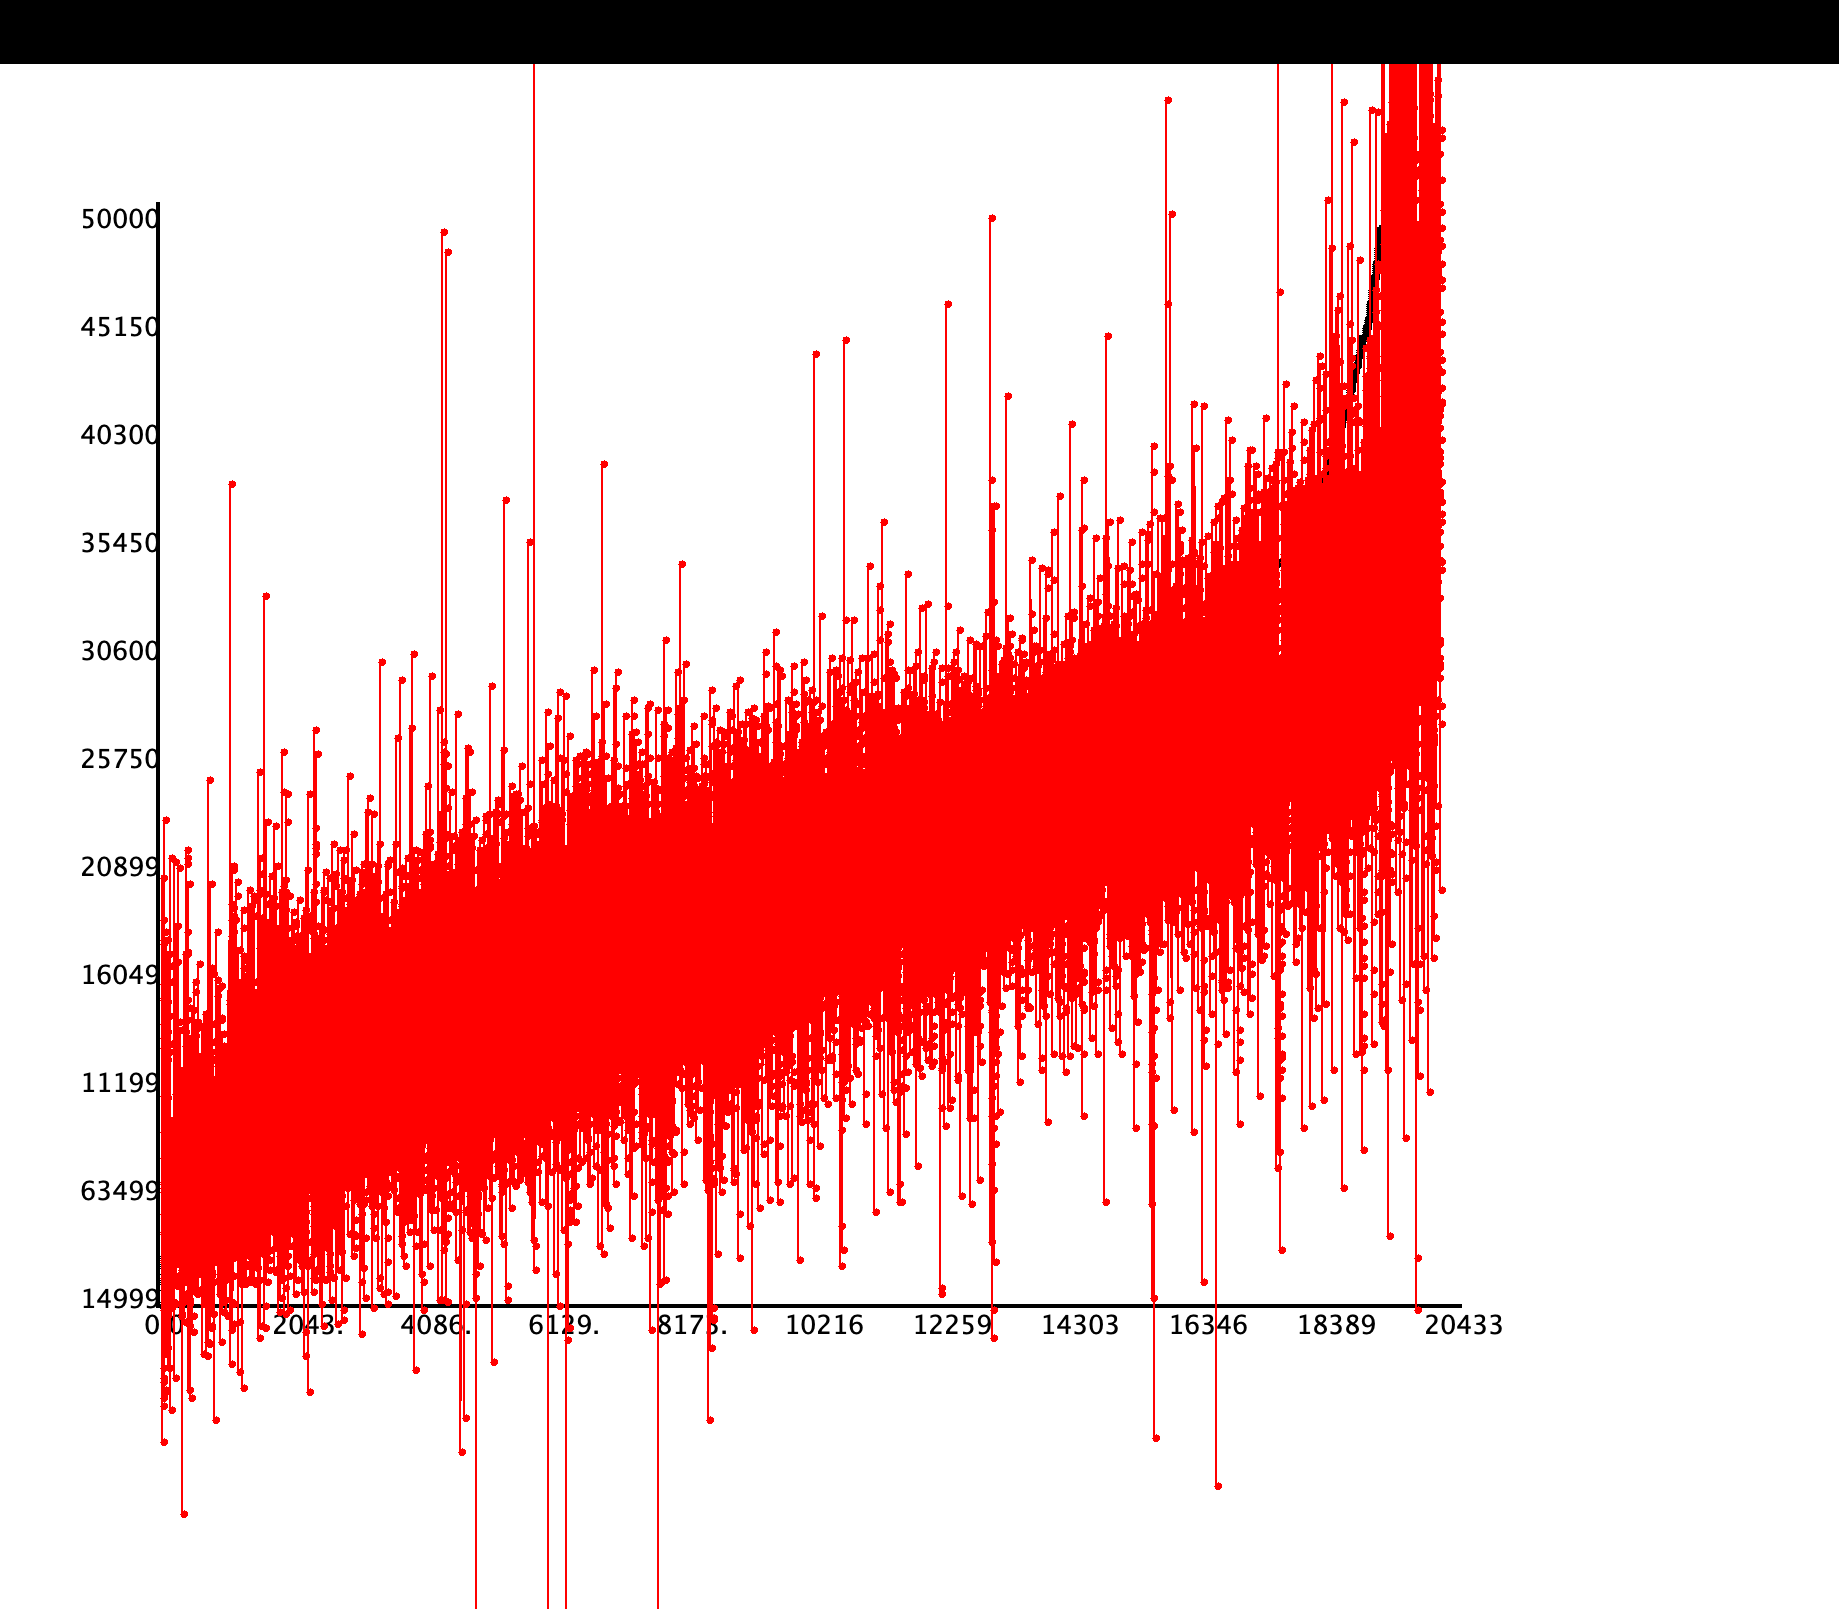
\includegraphics[width=\textwidth]{../House_Prices_Scalation_Plots/Scalation_Reg_In_Sample.png}
     \end{subfigure}
     \hfill
     \begin{subfigure}[b]{0.4\textwidth}
         \centering
         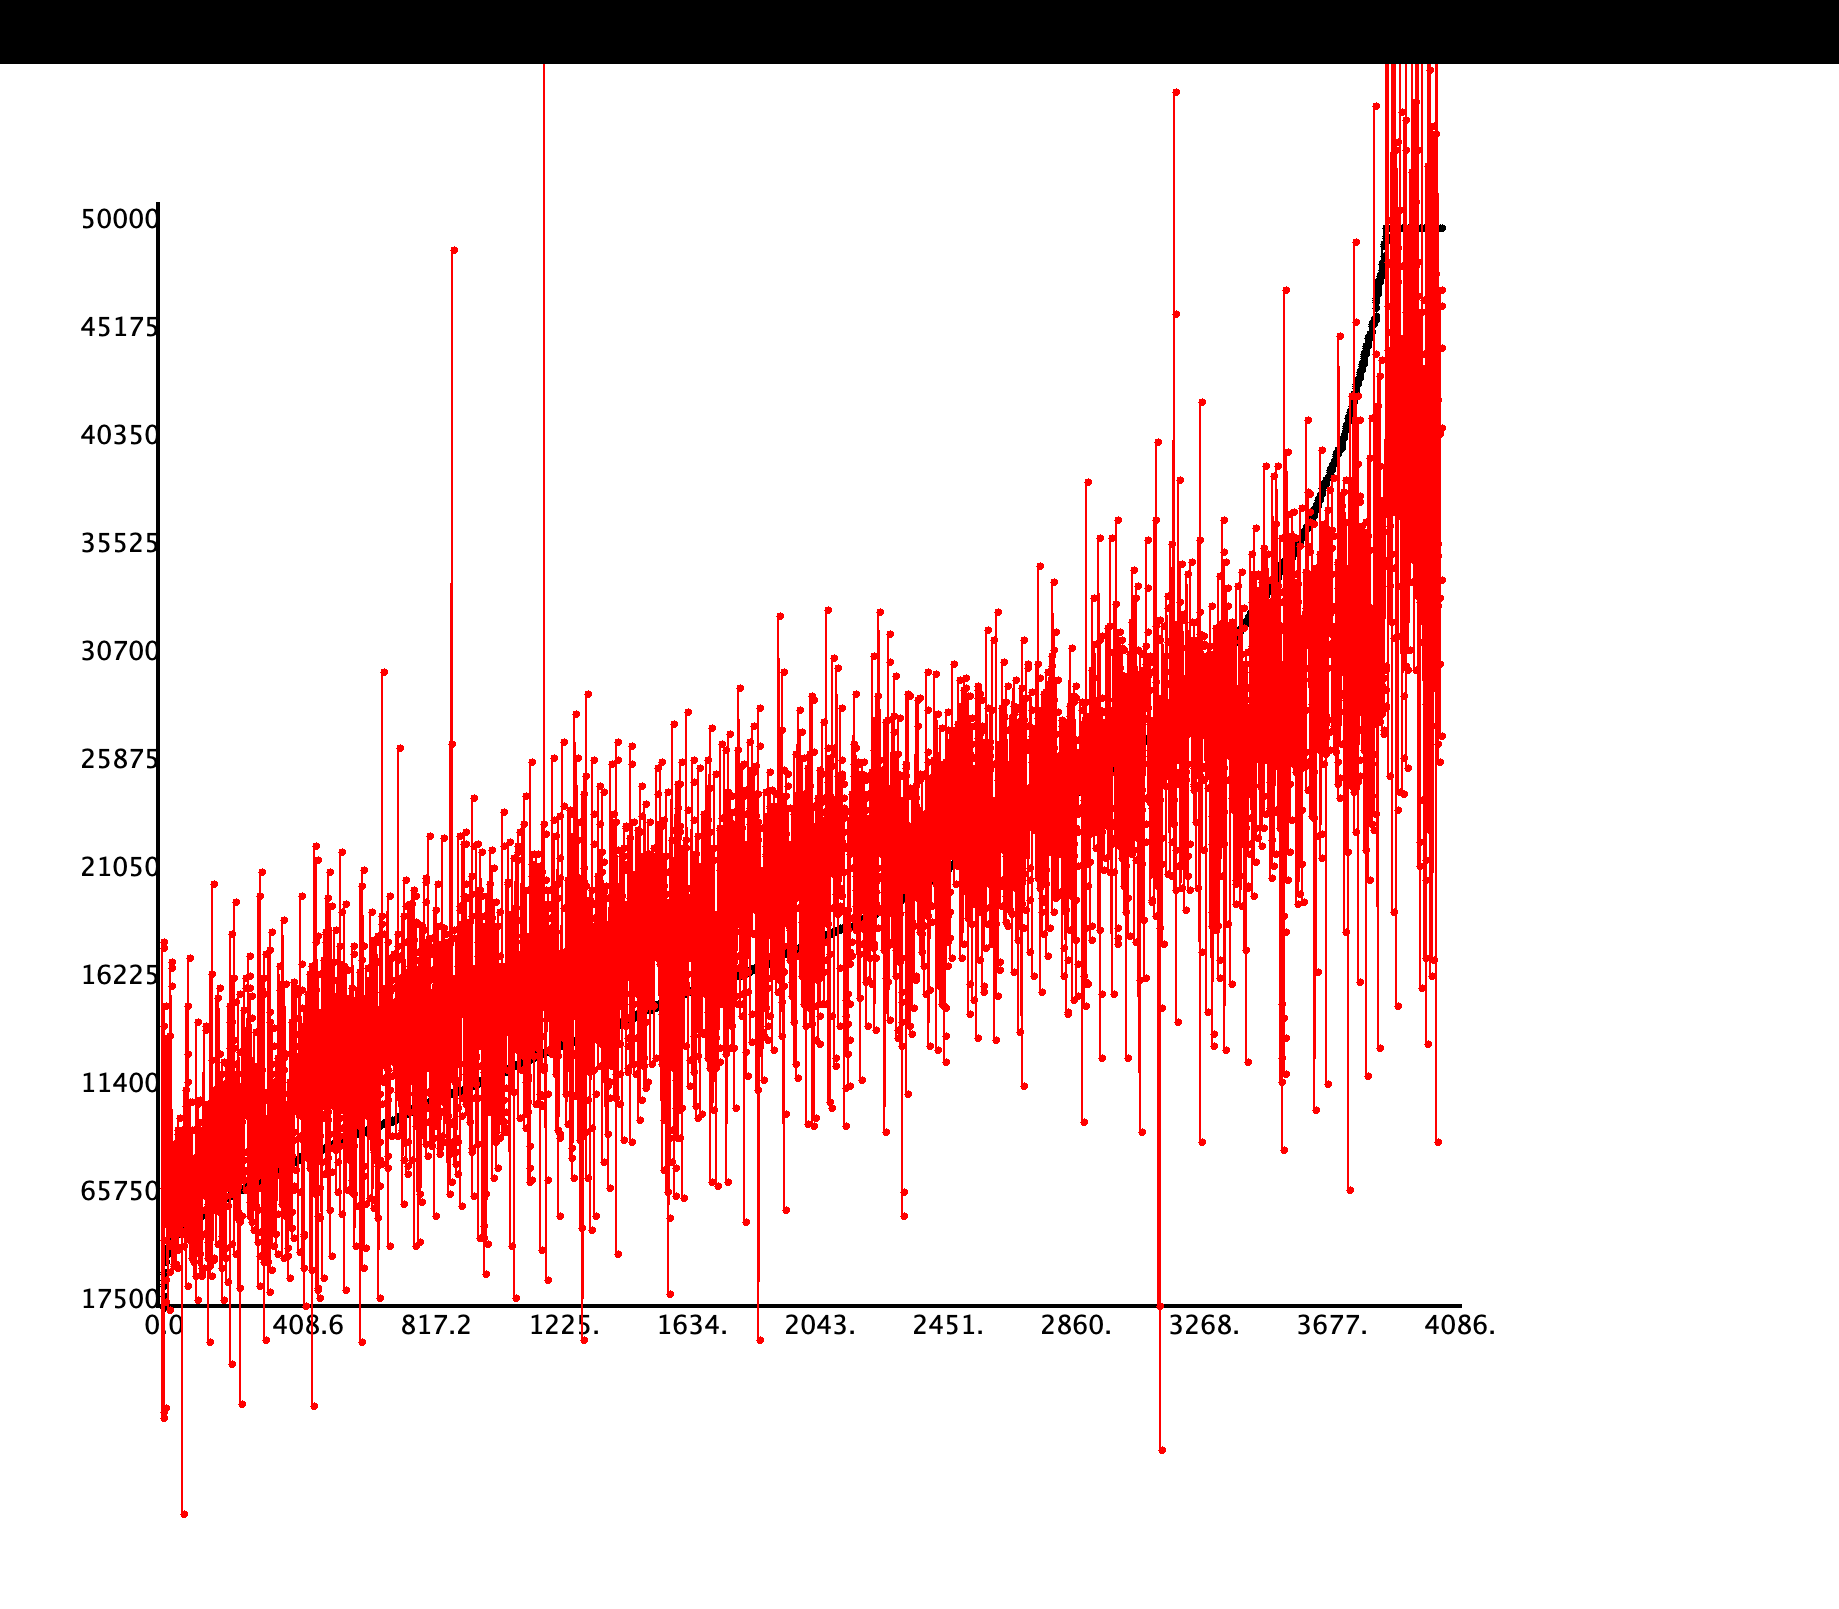
\includegraphics[width=\textwidth]{../House_Prices_Scalation_Plots/Scalation_Reg_80_20.png}
     \end{subfigure}

     \vspace{10pt} % Add some vertical spacing between rows

     % Second Row
     \begin{subfigure}[b]{0.49\textwidth}
         \centering
         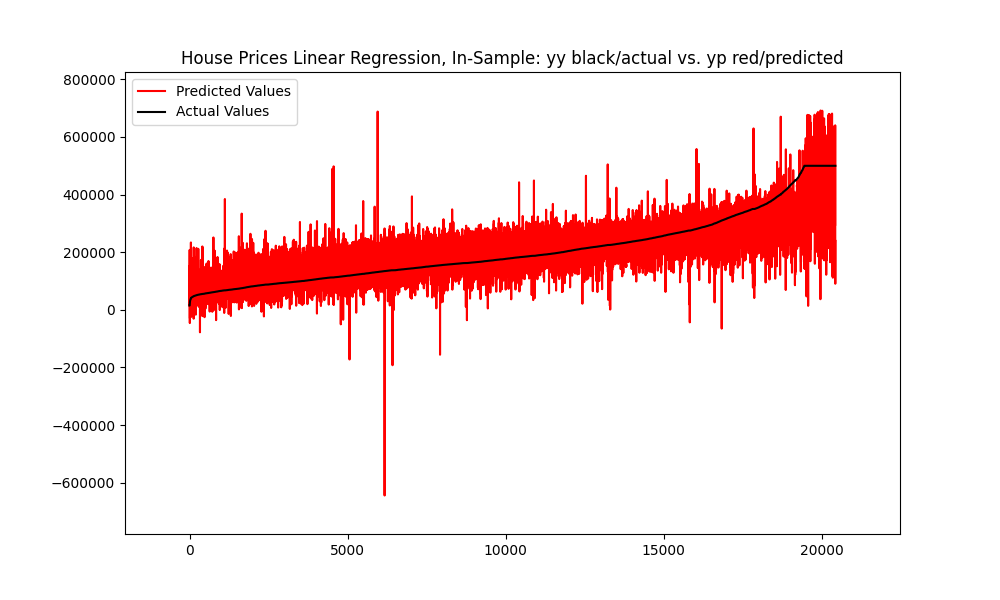
\includegraphics[width=\textwidth]{../House_Prices_Statsmodels_Plots/Statsmodels_Reg_In_Sample.png}
     \end{subfigure}
     \hfill
     \begin{subfigure}[b]{0.49\textwidth}
         \centering
         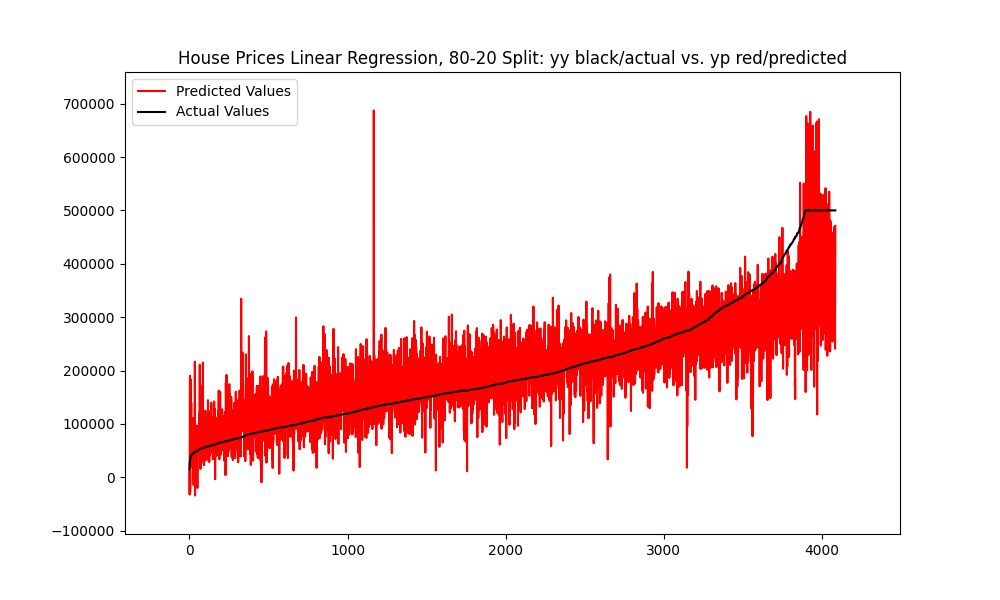
\includegraphics[width=\textwidth]{../House_Prices_Statsmodels_Plots/Statsmodels_Reg_80_20.png}
     \end{subfigure}
     
     \caption{California House Prices Linear Regression Plots\\ Top Left: Scalation In-Sample, Top Right: Scalation Out-of-Sample\\ Bottom Left: Statsmodels In-Sample, Bottom Right: Statsmodels Out-of-Sample\\ black: actual y-values, red: predicted y-values}
     \label{fig:California House Prices Linear Regression Plots}
\end{figure}

\subsubsection{Feature Selection}

Scalation Forward Selection: intercept, median income, ocean proximity INLAND, housing median age, total bedrooms, population, total rooms, households, ocean proximity ISLAND, latitude, longitude, ocean proximity NEAR BAY, ocean proximity NEAR OCEAN

Statsmodels Forward Selection: intercept, median income, ocean proximity INLAND, housing median age, total bedrooms, population, households, total rooms, ocean proximity NEAR OCEAN, longitude, latitude, ocean proximity ISLAND, ocean proximity NEAR BAY

\begin{figure}[H]
     \centering
     \captionsetup{justification=centering}
     % First Row
     \begin{subfigure}[b]{0.4\textwidth}
         \centering
         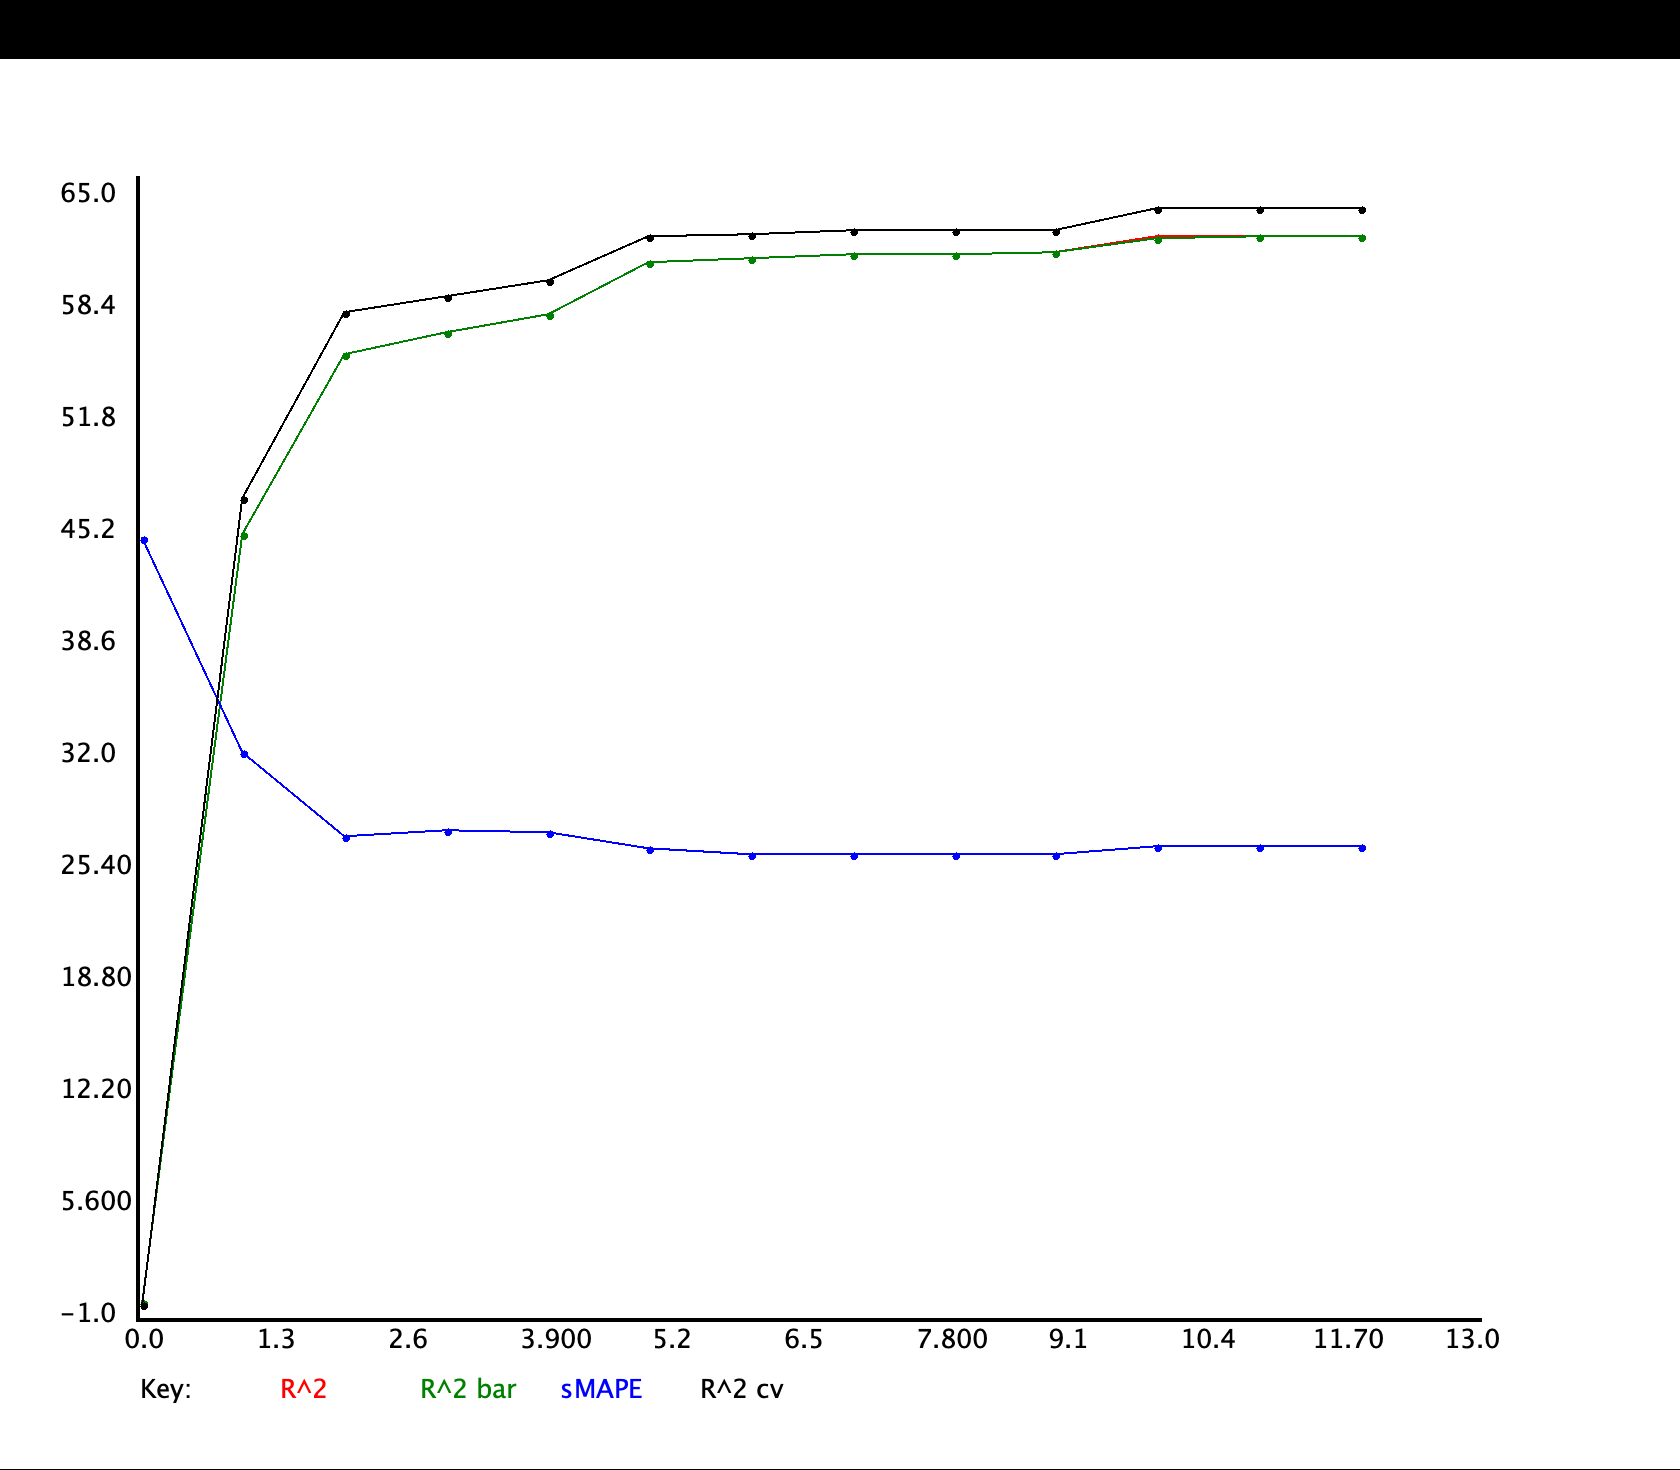
\includegraphics[width=\textwidth]{../House_Prices_Scalation_Plots/Scalation_Reg_rSq_Forward.png}
     \end{subfigure}
     \hfill
     \begin{subfigure}[b]{0.4\textwidth}
         \centering
         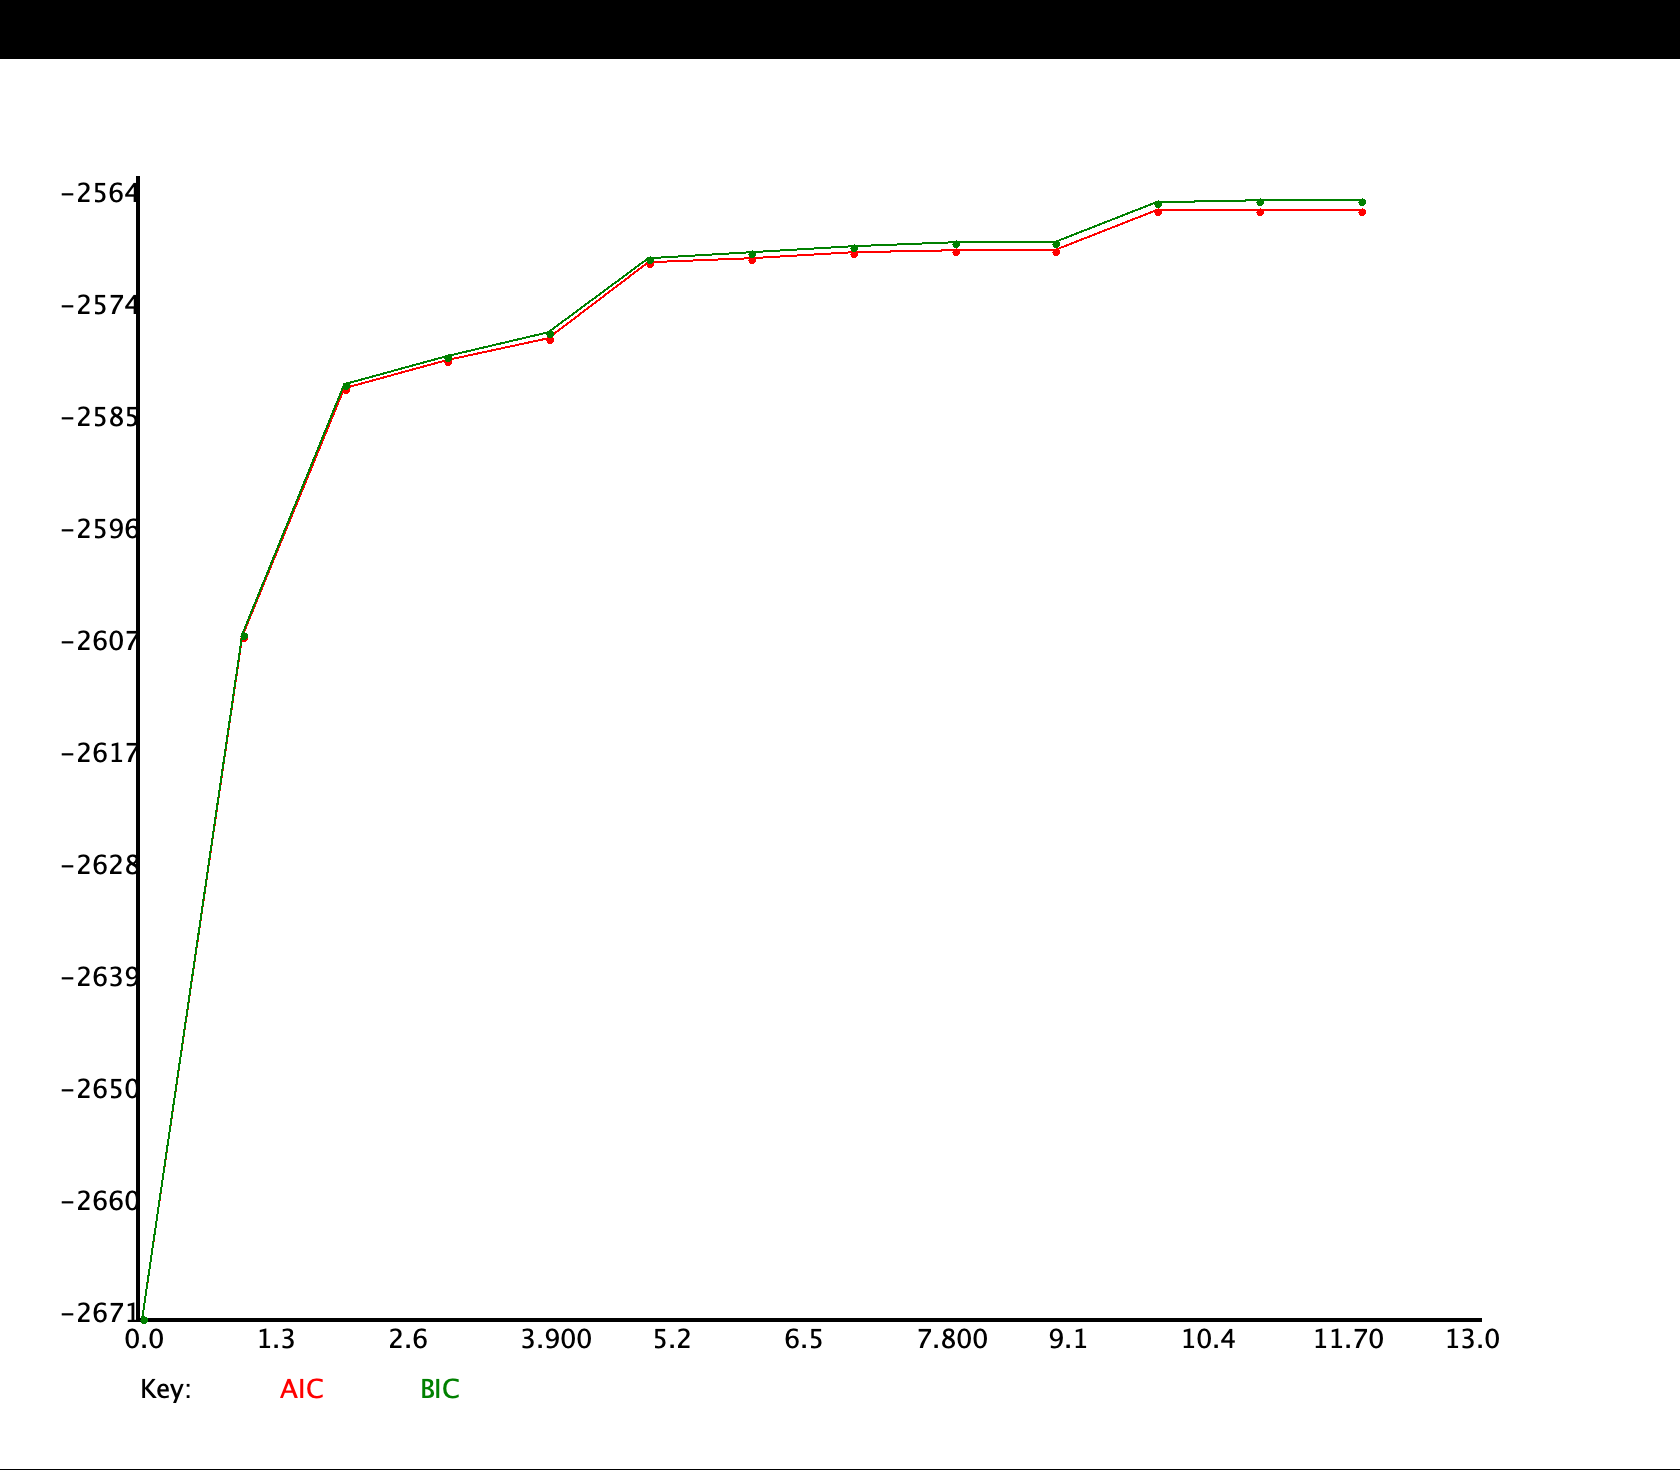
\includegraphics[width=\textwidth]{../House_Prices_Scalation_Plots/Scalation_Reg_AIC_BIC_Forward.png}
     \end{subfigure}

     \vspace{10pt} % Add some vertical spacing between rows

     % Second Row
     \begin{subfigure}[b]{0.49\textwidth}
         \centering
         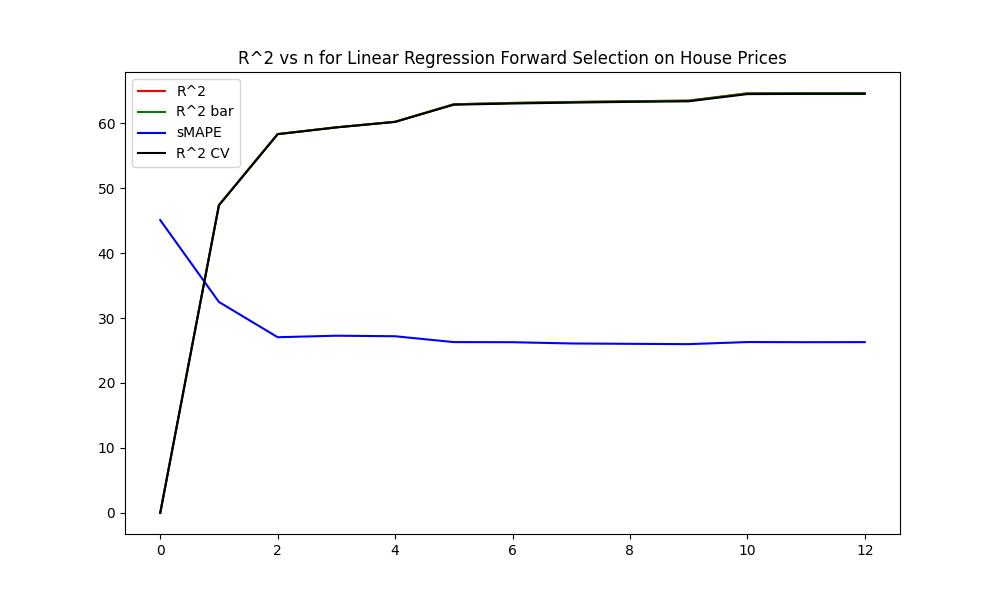
\includegraphics[width=\textwidth]{../House_Prices_Statsmodels_Plots/Statsmodels_Reg_rSq_Forward.png}
     \end{subfigure}
     \hfill
     \begin{subfigure}[b]{0.49\textwidth}
         \centering
         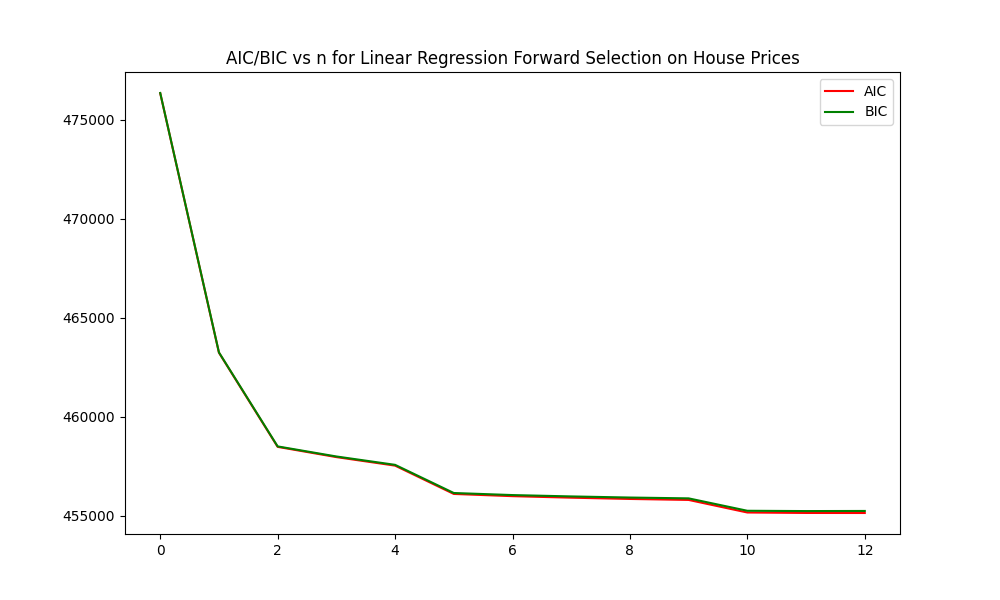
\includegraphics[width=\textwidth]{../House_Prices_Statsmodels_Plots/Statsmodels_Reg_AIC_BIC_Forward.png}
     \end{subfigure}
     
     \caption{California House Prices Linear Regression Forward Selection Quality of Fit Metrics\\ Top Left: Scalation $R^2$, Top Right: Scalation AIC/BIC\\ Bottom Left: Statsmodels $R^2$, Bottom Right: Statsmodels AIC/BIC}
     \label{fig:California House Prices Linear Regression Forward Selection Quality of Fit Metrics}
\end{figure}

Scalation Backward Elimination Reversed: intercept, median income, latitude, longitude, total bedrooms, population, housing median age, ocean proximity INLAND, total rooms, households, ocean proximity ISLAND, ocean proximity NEAR BAY, ocean proximity NEAR OCEAN

Statsmodels Backward Elimination Reversed: intercept, median income, latitude, longitude, total bedrooms, population, housing median age, ocean proximity INLAND, total rooms, households, ocean proximity ISLAND, ocean proximity NEAR OCEAN, ocean proximity NEAR BAY

\begin{figure}[H]
     \centering
     \captionsetup{justification=centering}
     % First Row
     \begin{subfigure}[b]{0.4\textwidth}
         \centering
         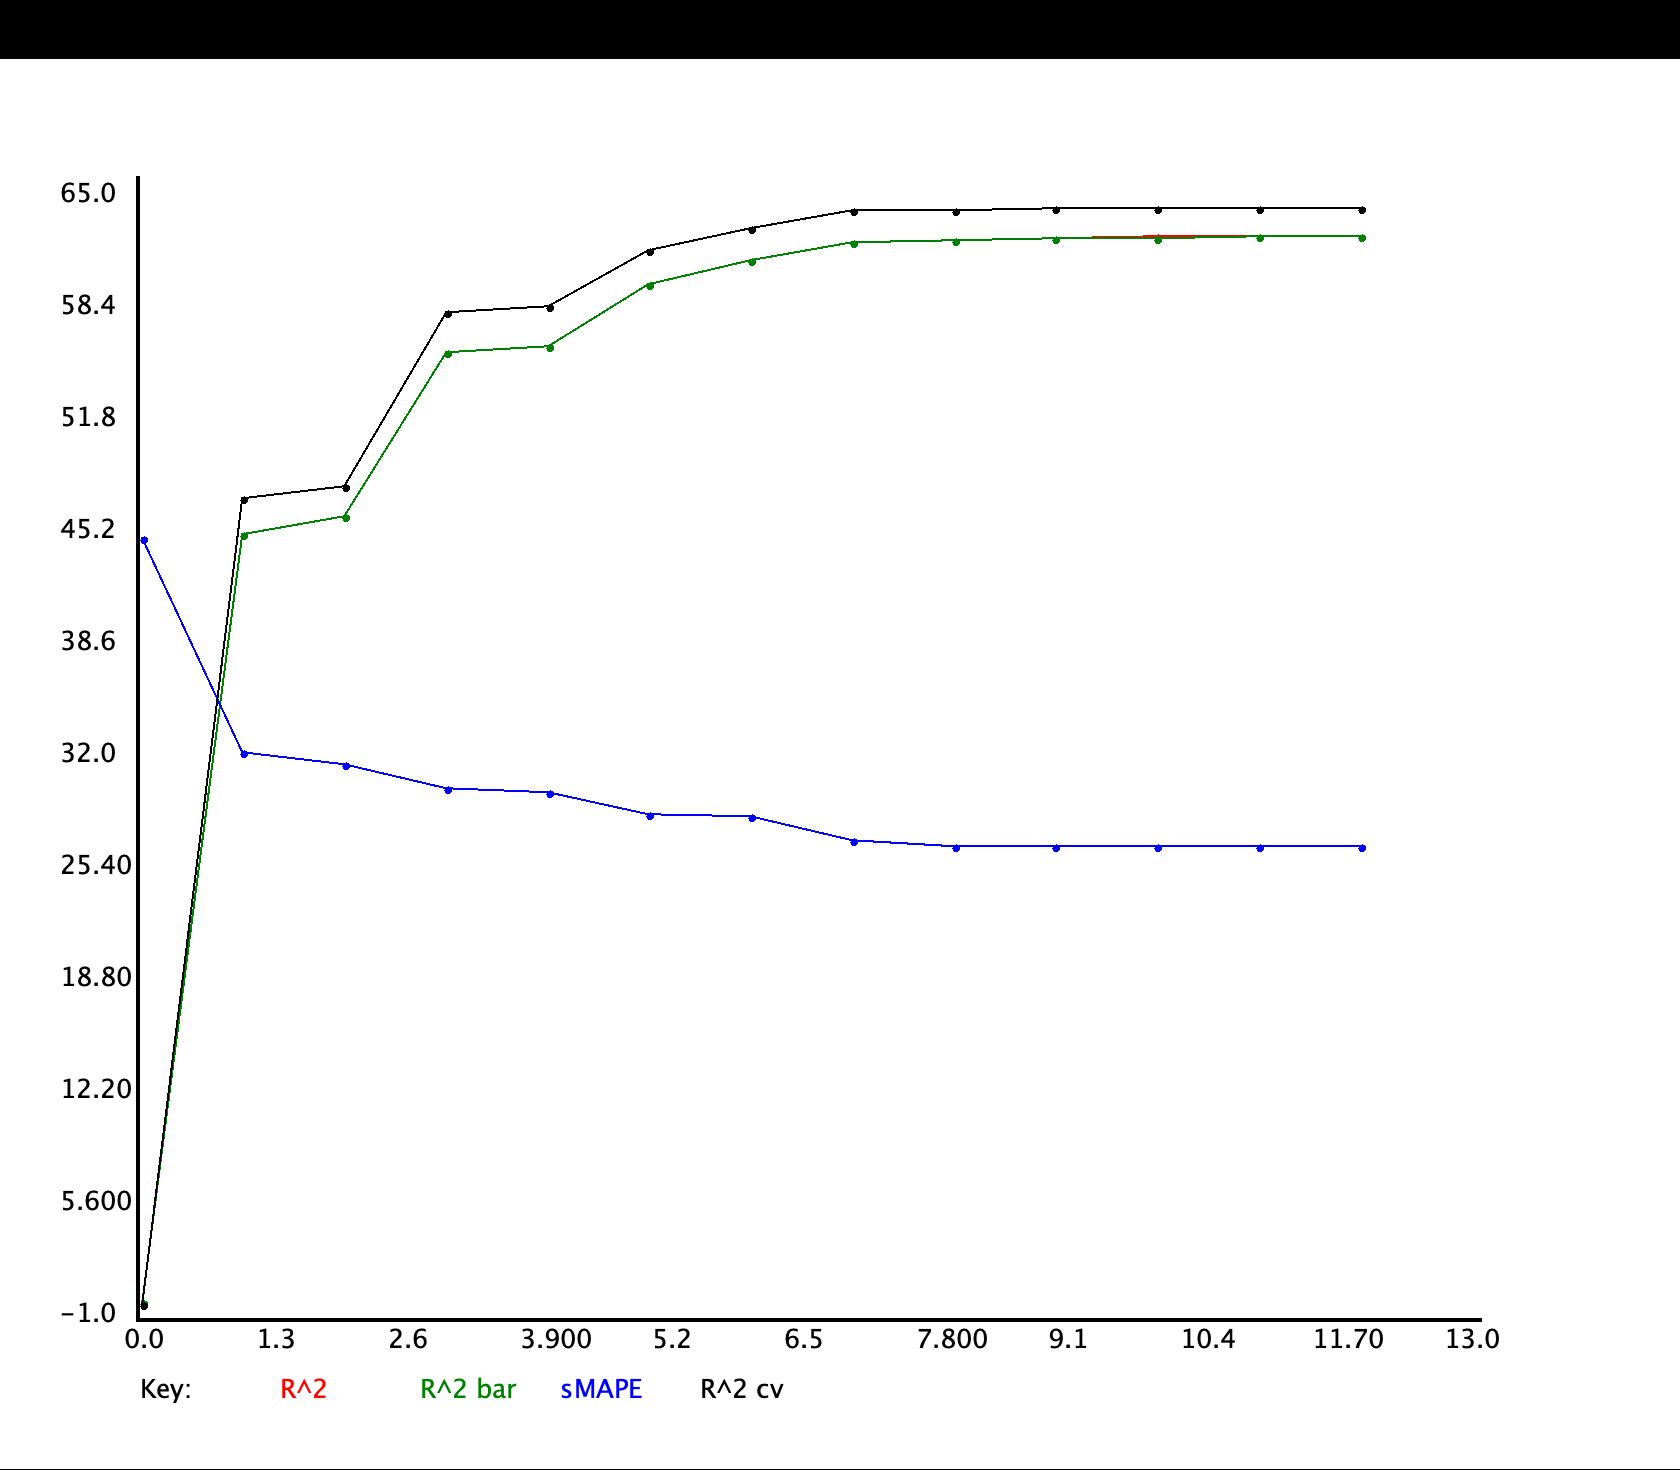
\includegraphics[width=\textwidth]{../House_Prices_Scalation_Plots/Scalation_Reg_rSq_Backward.png}
     \end{subfigure}
     \hfill
     \begin{subfigure}[b]{0.4\textwidth}
         \centering
         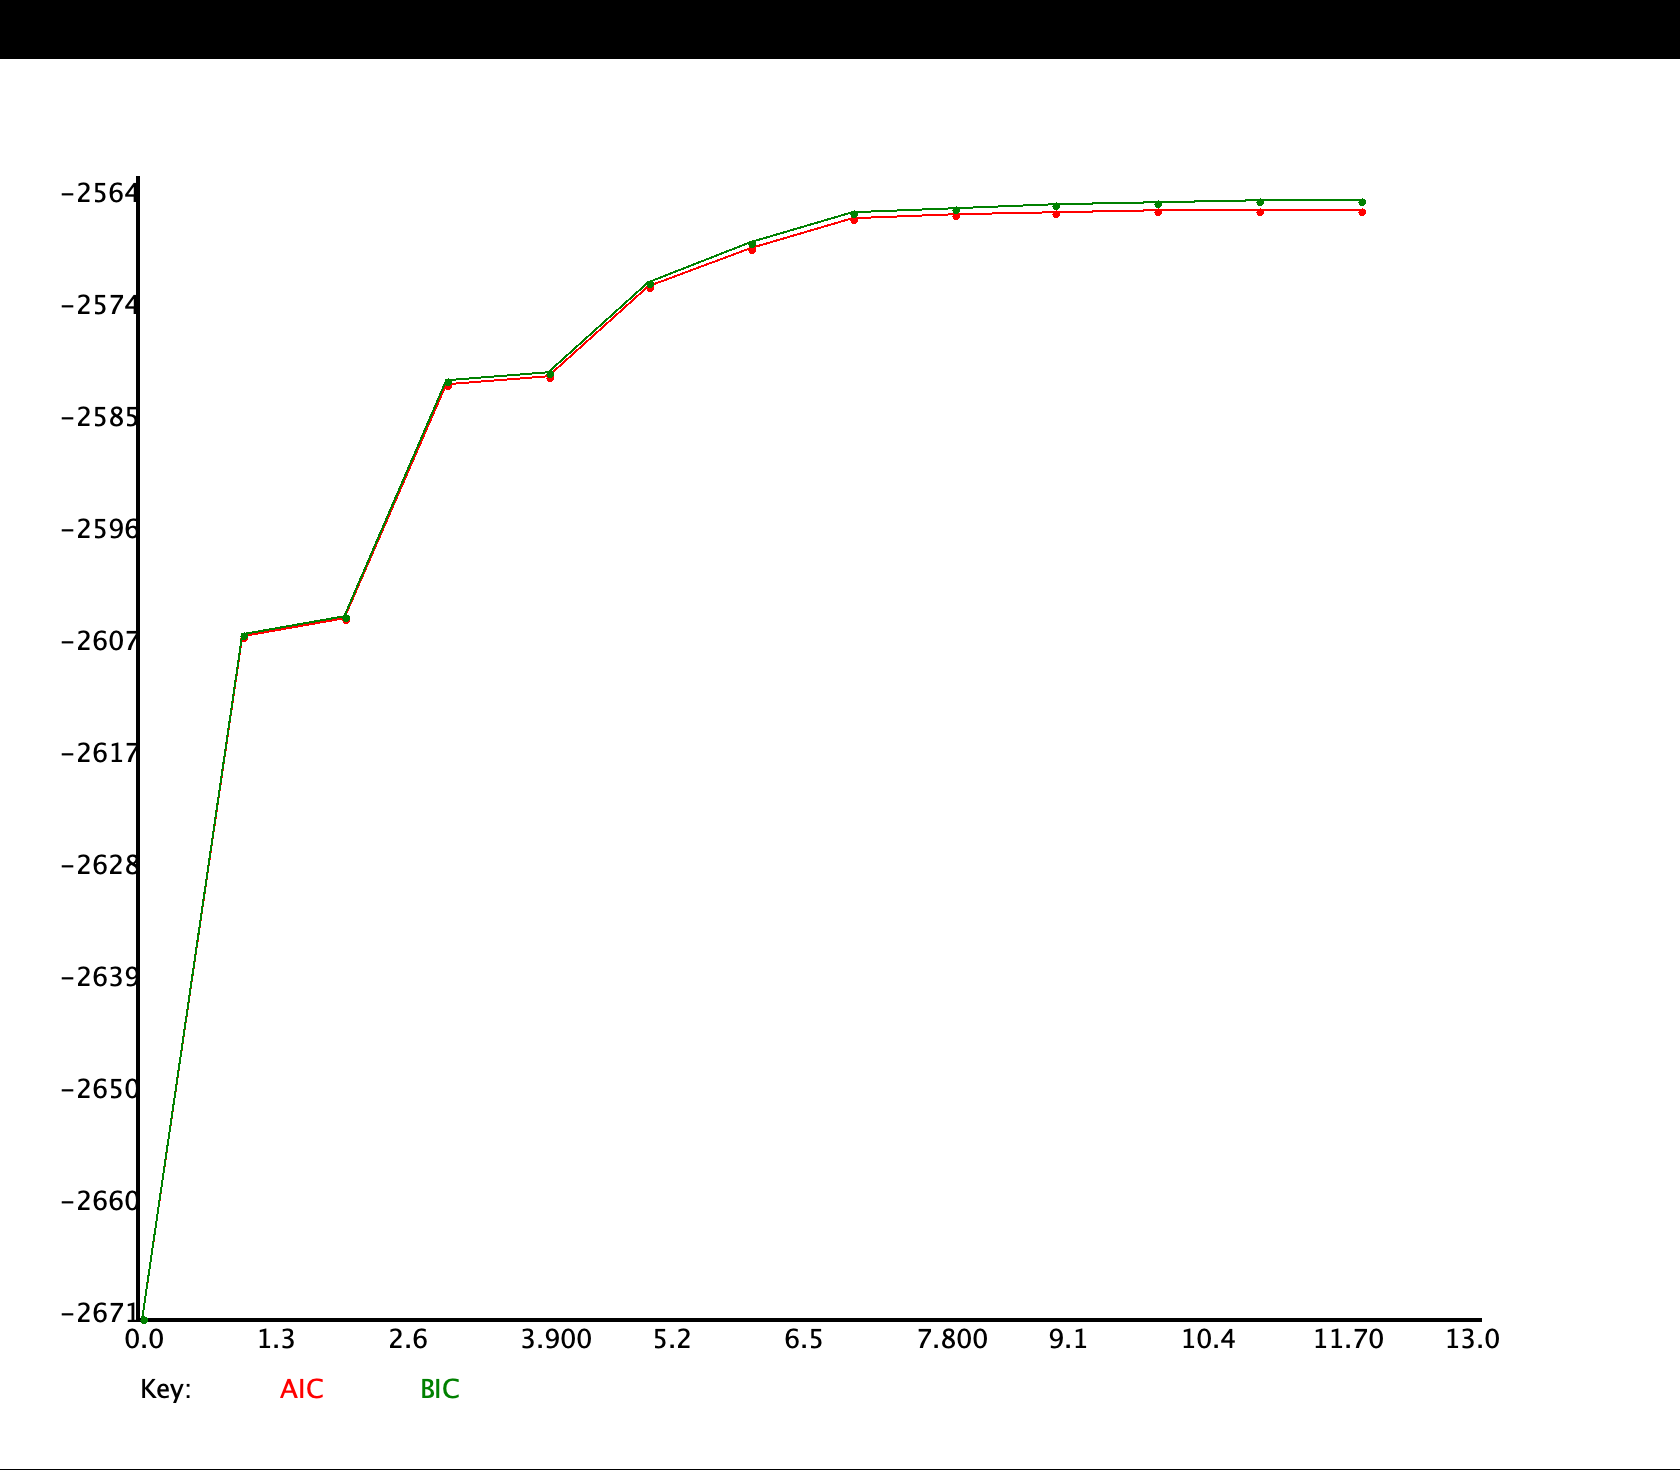
\includegraphics[width=\textwidth]{../House_Prices_Scalation_Plots/Scalation_Reg_AIC_BIC_Backward.png}
     \end{subfigure}

     \vspace{10pt} % Add some vertical spacing between rows

     % Second Row
     \begin{subfigure}[b]{0.49\textwidth}
         \centering
         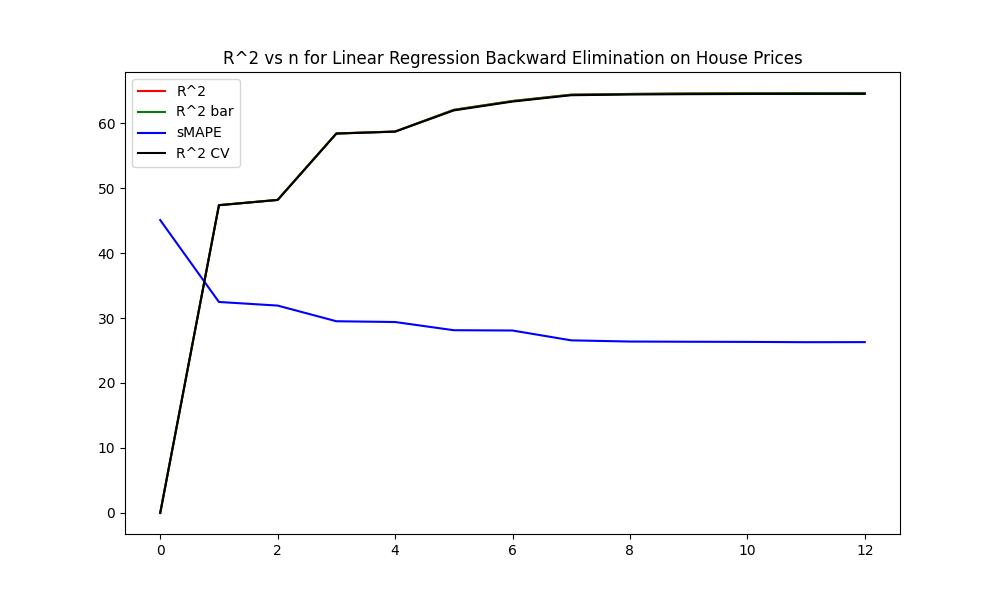
\includegraphics[width=\textwidth]{../House_Prices_Statsmodels_Plots/Statsmodels_Reg_rSq_Backward.png}
     \end{subfigure}
     \hfill
     \begin{subfigure}[b]{0.49\textwidth}
         \centering
         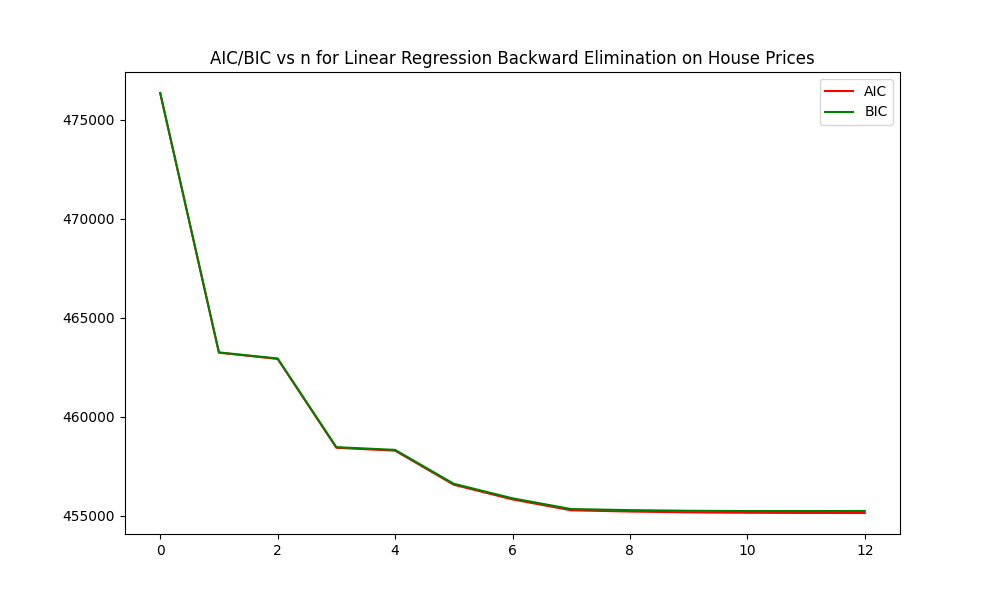
\includegraphics[width=\textwidth]{../House_Prices_Statsmodels_Plots/Statsmodels_Reg_AIC_BIC_Backward.png}
     \end{subfigure}
     
     \caption{California House Prices Linear Regression Reversed Backward Elimination Quality of Fit Metrics\\ Top Left: Scalation $R^2$, Top Right: Scalation AIC/BIC\\ Bottom Left: Statsmodels $R^2$, Bottom Right: Statsmodels AIC/BIC}
     \label{fig:California House Prices Linear Regression Reversed Backward Elimination Quality of Fit Metrics}
\end{figure}

Scalation Stepwise Selection: intercept, median income, ocean proximity INLAND, housing median age, total bedrooms, population, total rooms, households, ocean proximity ISLAND, latitude, longitude, ocean proximity NEAR BAY

Statsmodels Stepwise Selection: intercept, median income, ocean proximity INLAND, housing median age, total bedrooms, population, households, total rooms, ocean proximity NEAR OCEAN, longitude, latitude, ocean proximity ISLAND, ocean proximity NEAR BAY

\begin{figure}[H]
     \centering
     \captionsetup{justification=centering}
     % First Row
     \begin{subfigure}[b]{0.4\textwidth}
         \centering
         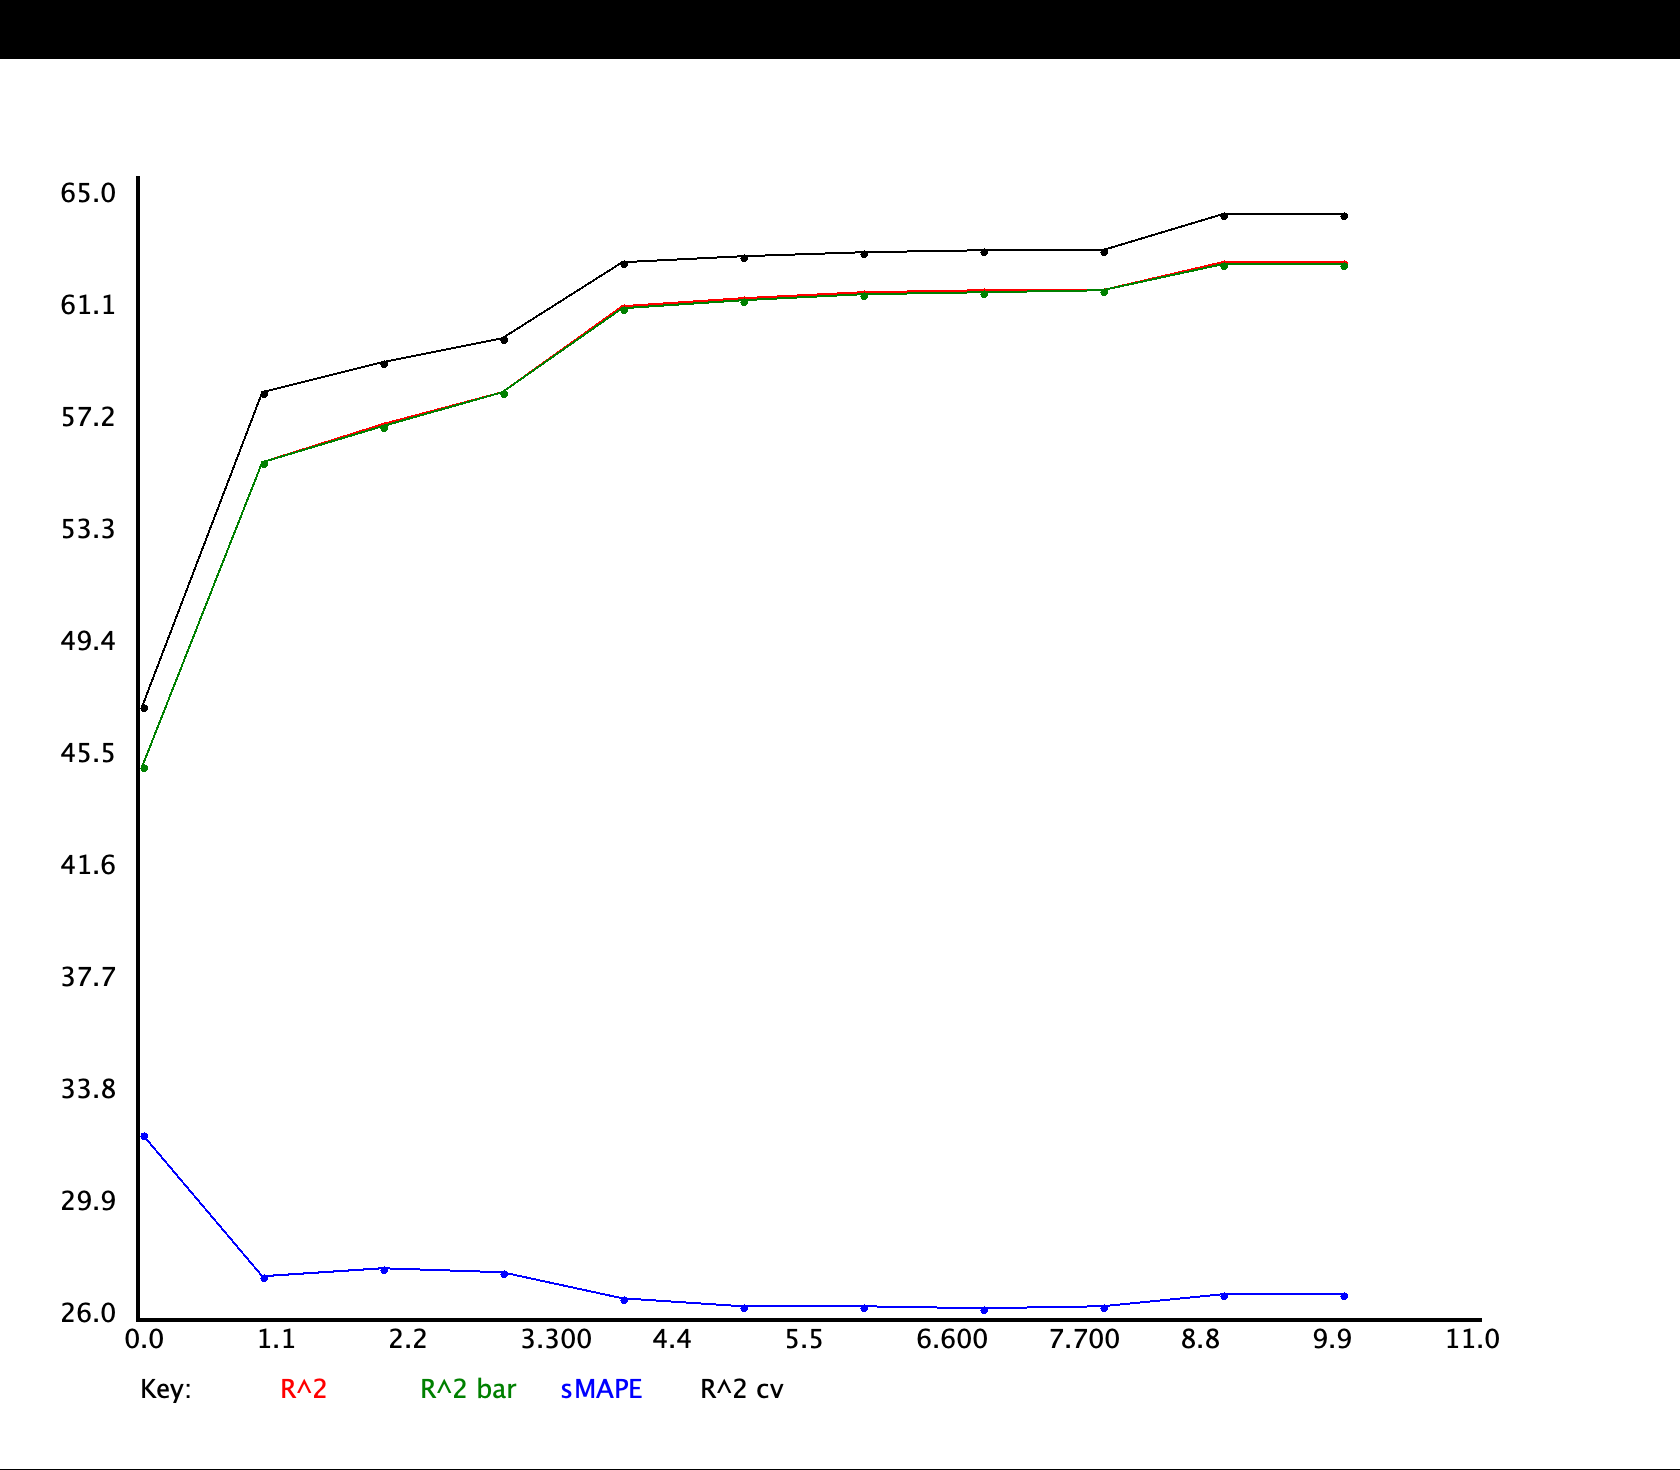
\includegraphics[width=\textwidth]{../House_Prices_Scalation_Plots/Scalation_Reg_rSq_Stepwise.png}
     \end{subfigure}
     \hfill
     \begin{subfigure}[b]{0.4\textwidth}
         \centering
         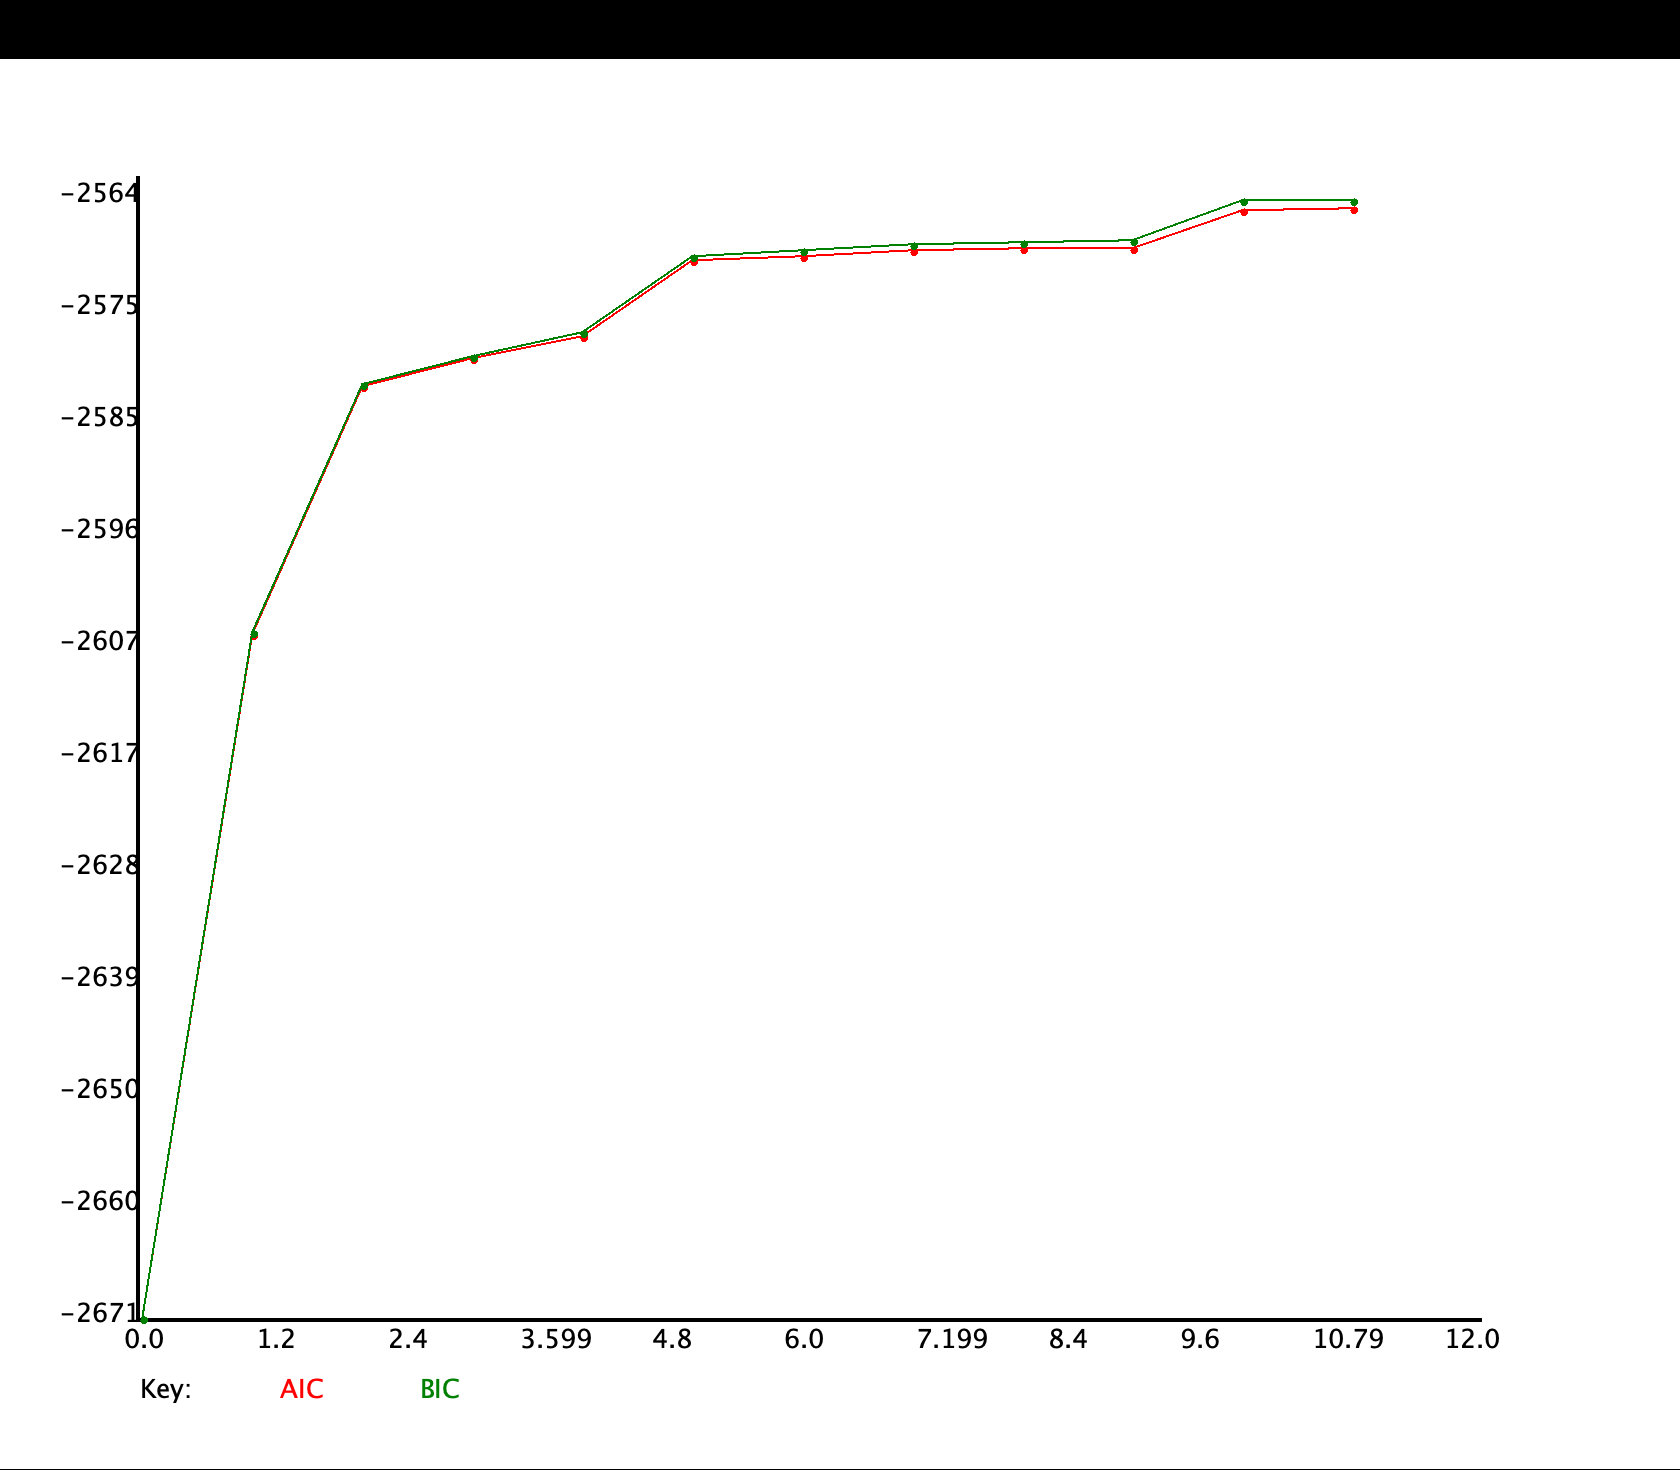
\includegraphics[width=\textwidth]{../House_Prices_Scalation_Plots/Scalation_Reg_AIC_BIC_Stepwise.png}
     \end{subfigure}

     \vspace{10pt} % Add some vertical spacing between rows

     % Second Row
     \begin{subfigure}[b]{0.49\textwidth}
         \centering
         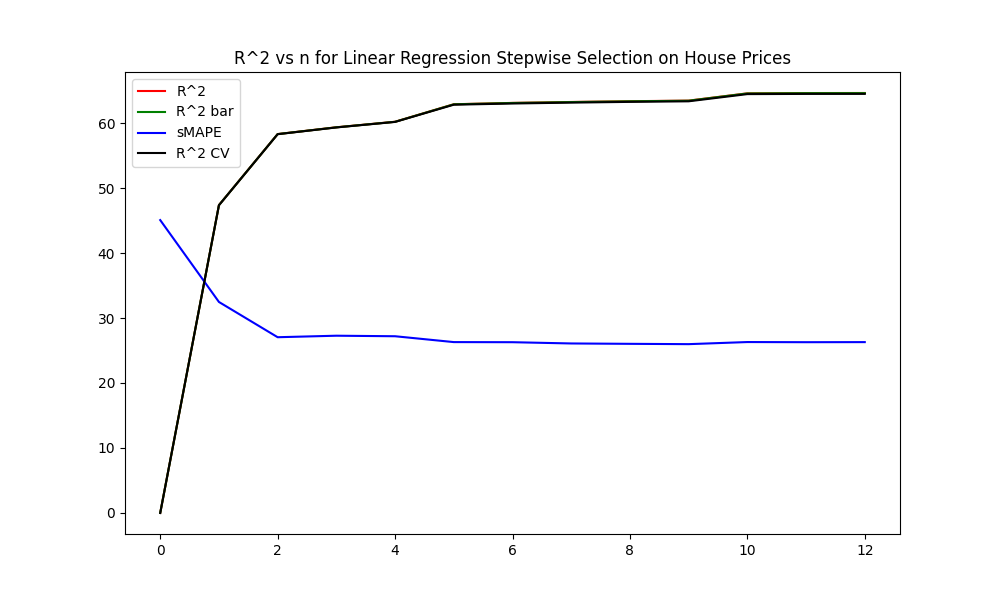
\includegraphics[width=\textwidth]{../House_Prices_Statsmodels_Plots/Statsmodels_Reg_rSq_Stepwise.png}
     \end{subfigure}
     \hfill
     \begin{subfigure}[b]{0.49\textwidth}
         \centering
         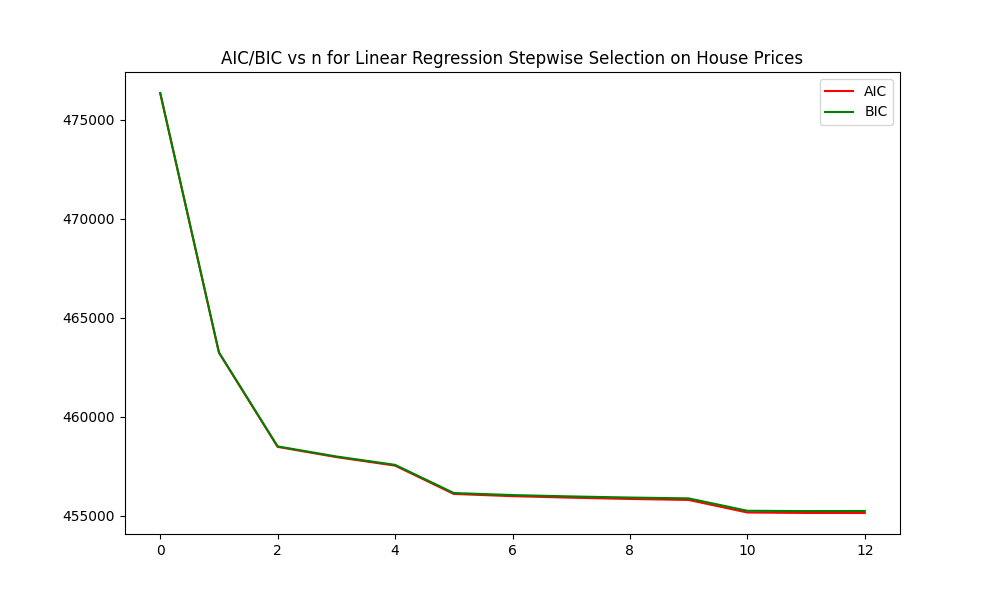
\includegraphics[width=\textwidth]{../House_Prices_Statsmodels_Plots/Statsmodels_Reg_AIC_BIC_Stepwise.png}
     \end{subfigure}
     
     \caption{California House Prices Linear Regression Stepwise Selection Quality of Fit Metrics\\ Top Left: Scalation $R^2$, Top Right: Scalation AIC/BIC\\ Bottom Left: Statsmodels $R^2$, Bottom Right: Statsmodels AIC/BIC}
     \label{fig:California House Prices Linear Regression Stepwise Selection Quality of Fit Metrics}
\end{figure}

\subsection{Ridge Regression}

\subsubsection{Quality of Fit}

Scalation California House Prices Ridge Lambda Used: $4.5$

\noindent Statsmodels California House Prices Ridge alpha Used: $0.00075$

\begin{table}[H]
\centering
\caption{Scalation - California House Prices Ridge Regression}
\label{tab:Scalation - House Prices Ridge Regression}
\begin{tabular}{|c|c|c|} \hline 
Metric & In-Sample & 80-20 Split \\ \hline \hline 
rSq &0.646187 & 0.643030 \\ \hline 
rSqBar &0.645979 &      0.642820 \\ \hline 
sst &2.72264e+14 &      5.31945e+13 \\ \hline 
sse &9.63306e+13 &      1.89888e+13 \\ \hline 
sde &68663.6 &  68138.8 \\ \hline 
mse0 &4.71446e+09 &     4.64729e+09 \\ \hline 
rmse &68662.0 & 68171.1 \\ \hline 
mae &49770.7 &  49547.5 \\ \hline 
smape &84.1956 &        83.7465 \\ \hline 
m &20433.0 &    4086.00 \\ \hline 
dfr &12.0000 &  12.0000 \\ \hline 
df &20420.0 &   20420.0 \\ \hline 
fStat &3107.84 &        3065.31 \\ \hline 
aic &-256528 &  -51248.0 \\ \hline 
bic &-256425 &  -51165.9 \\ \hline 
\end{tabular}
\end{table}

\begin{table}[H]
\centering
\caption{Statsmodels - California House Prices Ridge Regression}
\label{tab:Statsmodels - House Prices Ridge Regression}
\begin{tabular}{|c|c|c|}\hline
Metric & In-Sample & 80-20 Split \\ \hline \hline
rSq & 0.6465 & 0.6526 \\ \hline
rSqBar & 0.6463 & 0.6517 \\ \hline
sst & 272264434648930.1562 & 54723646809444.8438 \\ \hline
sse & 96258299438945.0312 & 19010019798780.8008 \\ \hline
sde & 68656.3308 & 68301.0654 \\ \hline
mse0 & 4710923478.6348 & 4651338340.7832 \\ \hline
rmse & 68636.1674 & 68200.7210 \\ \hline
mae & 49740.8323 & 49948.3752 \\ \hline
smape & 84.1934 & 84.5004 \\ \hline
m & 20433.0000 & 4087.0000 \\ \hline
dfr & 12.0000 & 12.0000 \\ \hline
df & 20421.0000 & 4075.0000 \\ \hline
fStat & 3111.6116 & 637.9663 \\ \hline
aic & 455131.2697 & 91002.3399 \\ \hline
bic & 455226.3686 & 91078.1267 \\ \hline
\end{tabular}
\end{table}

\begin{table}[H]
\centering
\caption{Scalation - California House Prices Ridge Regression CV}
\label{tab:Scalation - California House Prices Ridge Regression CV}
\begin{tabular}{|c|c|c|c|c|c|}\hline
Metric & num folds & min & max & mean & stdev \\ \hline \hline
rSq & 5 & 0.628 & 0.661 & 0.645 & 0.012 \\ \hline
rSqBar & 5 & 0.628 & 0.661 & 0.645 & 0.012 \\ \hline
sst & 5 & 53194492241132.950 & 57310203956797.310 & 54411355017051.120 & 1675890609057.038 \\ \hline
sse & 5 & 18091667336305.707 & 21292685629304.570 & 19337767834684.273 & 1200174049699.611 \\ \hline
sde & 5 & 66545.874 & 72132.543 & 68755.187 & 2089.324 \\ \hline
mse0 & 5 & 4427720836.100 & 5211132067.867 & 4732689142.116 & 293728352.839 \\ \hline
rmse & 5 & 66541.121 & 72188.171 & 68768.621 & 2111.271 \\ \hline
mae & 5 & 48571.829 & 51936.142 & 49824.251 & 1278.386 \\ \hline
smape & 5 & 83.028 & 85.867 & 84.269 & 1.082 \\ \hline
m & 5 & 4086.000 & 4086.000 & 4086.000 & 0.000 \\ \hline
dfr & 5 & 12.000 & 12.000 & 12.000 & 0.000 \\ \hline
df & 5 & 20420.000 & 20420.000 & 20420.000 & 0.000 \\ \hline
fStat & 5 & 2878.444 & 3321.418 & 3093.974 & 162.831 \\ \hline
aic & 5 & -51496.212 & -51151.405 & -51285.632 & 129.280 \\ \hline
bic & 5 & -51414.112 & -51069.306 & -51203.533 & 129.280 \\ \hline
\end{tabular}
\end{table}

\begin{table}[H]
\centering
\caption{Statsmodels - California House Prices Ridge Regression CV}
\label{tab:Statsmodels - California House Prices Ridge Regression CV}
\begin{tabular}{|c|c|c|c|c|c|}\hline
Metric & num folds & min & max & mean & stdev \\ \hline \hline
rSq & 5 & 0.6200 & 0.6552 & 0.6451 & 0.0128 \\ \hline
rSqBar & 5 & 0.6190 & 0.6542 & 0.6442 & 0.0128 \\ \hline
sst & 5 & 53541750406767.3438 & 54912923487891.5859 & 54447676367709.7031 & 499826929365.4294 \\ \hline
sse & 5 & 18936343352953.6953 & 20346351773710.8438 & 19315930669616.9062 & 529559988044.9923 \\ \hline
sde & 5 & 68168.5809 & 70669.6210 & 68845.4795 & 937.8696 \\ \hline
mse0 & 5 & 4633311317.0917 & 4979528089.5034 & 4726659263.5018 & 129909580.1956 \\ \hline
rmse & 5 & 68068.4311 & 70565.7714 & 68744.3253 & 936.4847 \\ \hline
mae & 5 & 49022.4983 & 50392.4501 & 49787.6622 & 446.3236 \\ \hline
smape & 5 & 82.7776 & 85.5287 & 84.2289 & 0.8846 \\ \hline
m & 5 & 4086.0000 & 4087.0000 & 4086.6000 & 0.4899 \\ \hline
dfr & 5 & 12.0000 & 12.0000 & 12.0000 & 0.0000 \\ \hline
df & 5 & 4074.0000 & 4075.0000 & 4074.6000 & 0.4899 \\ \hline
fStat & 5 & 553.8997 & 645.1640 & 618.4713 & 33.0113 \\ \hline
aic & 5 & 90978.1773 & 91258.6635 & 91057.5665 & 104.7583 \\ \hline
bic & 5 & 91053.9612 & 91334.4474 & 91133.3521 & 104.7576 \\ \hline
\end{tabular}
\end{table}

\begin{figure}[H]
     \centering
     \captionsetup{justification=centering}
     % First Row
     \begin{subfigure}[b]{0.4\textwidth}
         \centering
         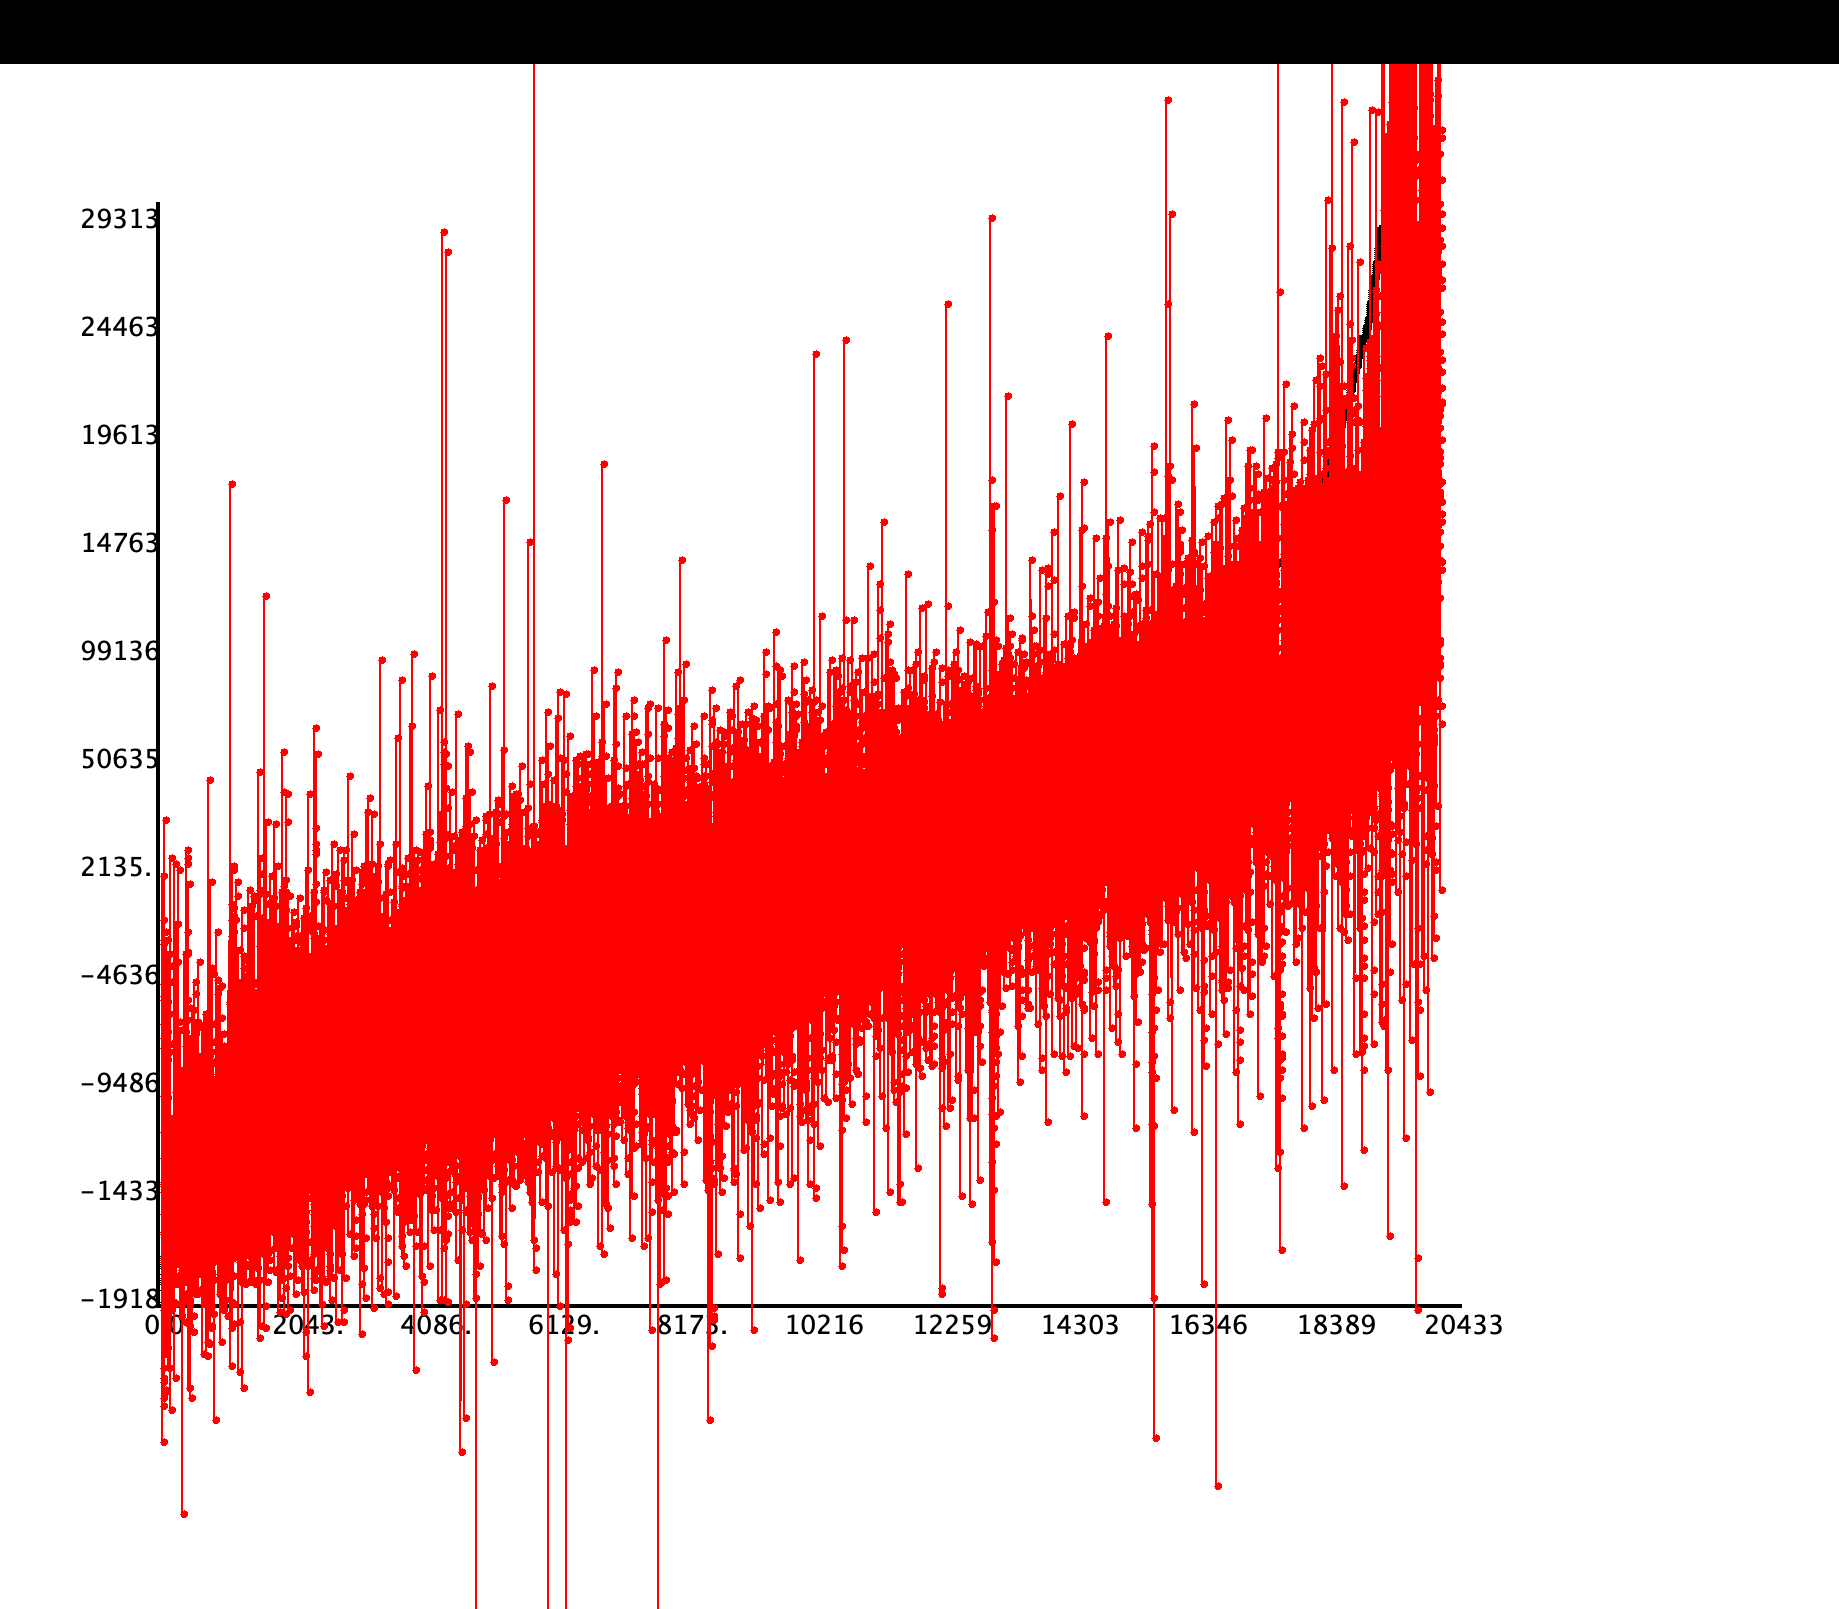
\includegraphics[width=\textwidth]{../House_Prices_Scalation_Plots/Scalation_Ridge_In_Sample.png}
     \end{subfigure}
     \hfill
     \begin{subfigure}[b]{0.4\textwidth}
         \centering
         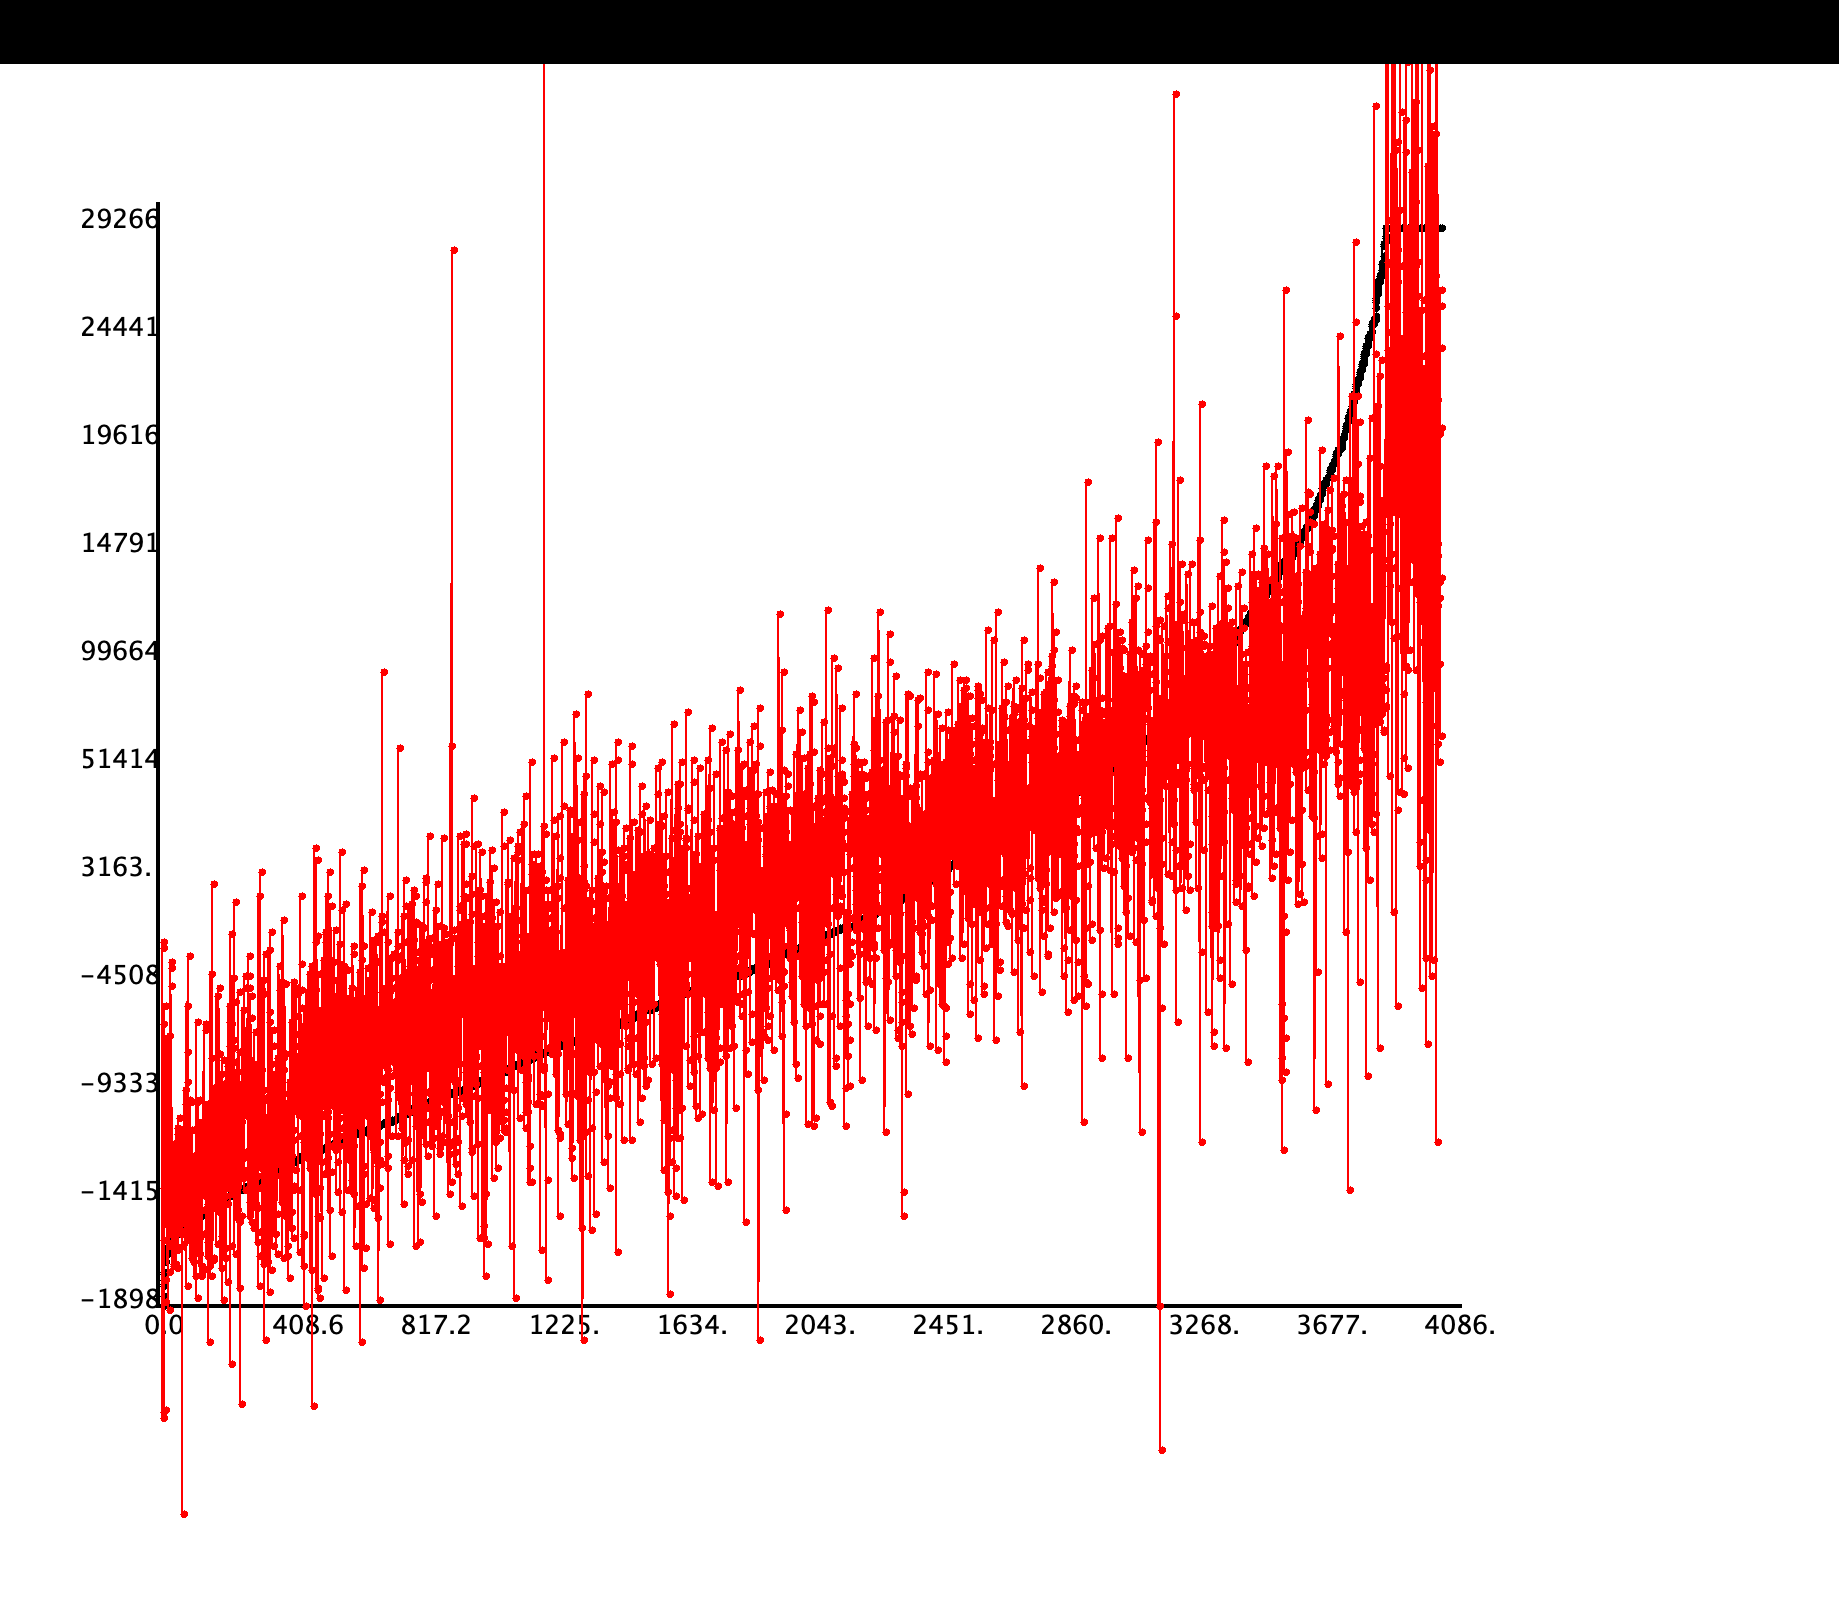
\includegraphics[width=\textwidth]{../House_Prices_Scalation_Plots/Scalation_Ridge_80_20.png}
     \end{subfigure}

     \vspace{10pt} % Add some vertical spacing between rows

     % Second Row
     \begin{subfigure}[b]{0.49\textwidth}
         \centering
         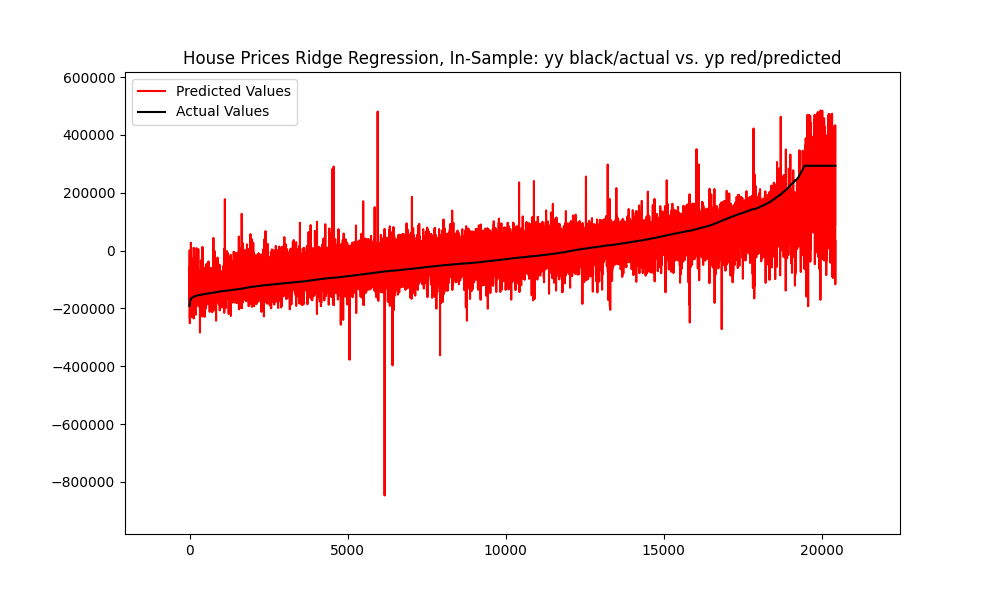
\includegraphics[width=\textwidth]{../House_Prices_Statsmodels_Plots/Statsmodels_Ridge_In_Sample.png}
     \end{subfigure}
     \hfill
     \begin{subfigure}[b]{0.49\textwidth}
         \centering
         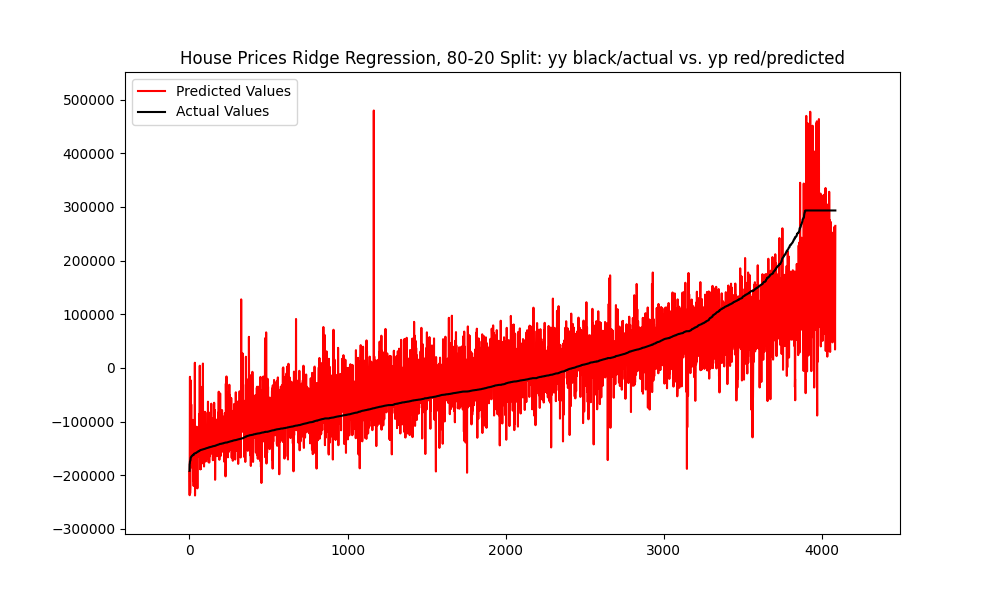
\includegraphics[width=\textwidth]{../House_Prices_Statsmodels_Plots/Statsmodels_Ridge_80_20.png}
     \end{subfigure}
     
     \caption{California House Prices Ridge Regression Plots\\ Top Left: Scalation In-Sample, Top Right: Scalation Out-of-Sample\\ Bottom Left: Statsmodels In-Sample, Bottom Right: Statsmodels Out-of-Sample\\ black: actual y-values, red: predicted y-values}
     \label{fig:California House Prices Ridge Regression Plots}
\end{figure}

\subsubsection{Feature Selection}

Scalation Forward Selection: longitude, total rooms, population, total bedrooms, households, latitude, median income, housing median age, ocean proximity INLAND, ocean proximity ISLAND, ocean proximity NEAR BAY, ocean proximity NEAR OCEAN

Statsmodels Forward Selection: Null, median income, ocean proximity INLAND, housing median age, total bedrooms, population, households, total rooms, ocean proximity NEAR OCEAN, longitude, latitude, ocean proximity ISLAND, ocean proximity NEAR BAY

\begin{figure}[H]
     \centering
     \captionsetup{justification=centering}
     % First Row
     \begin{subfigure}[b]{0.4\textwidth}
         \centering
         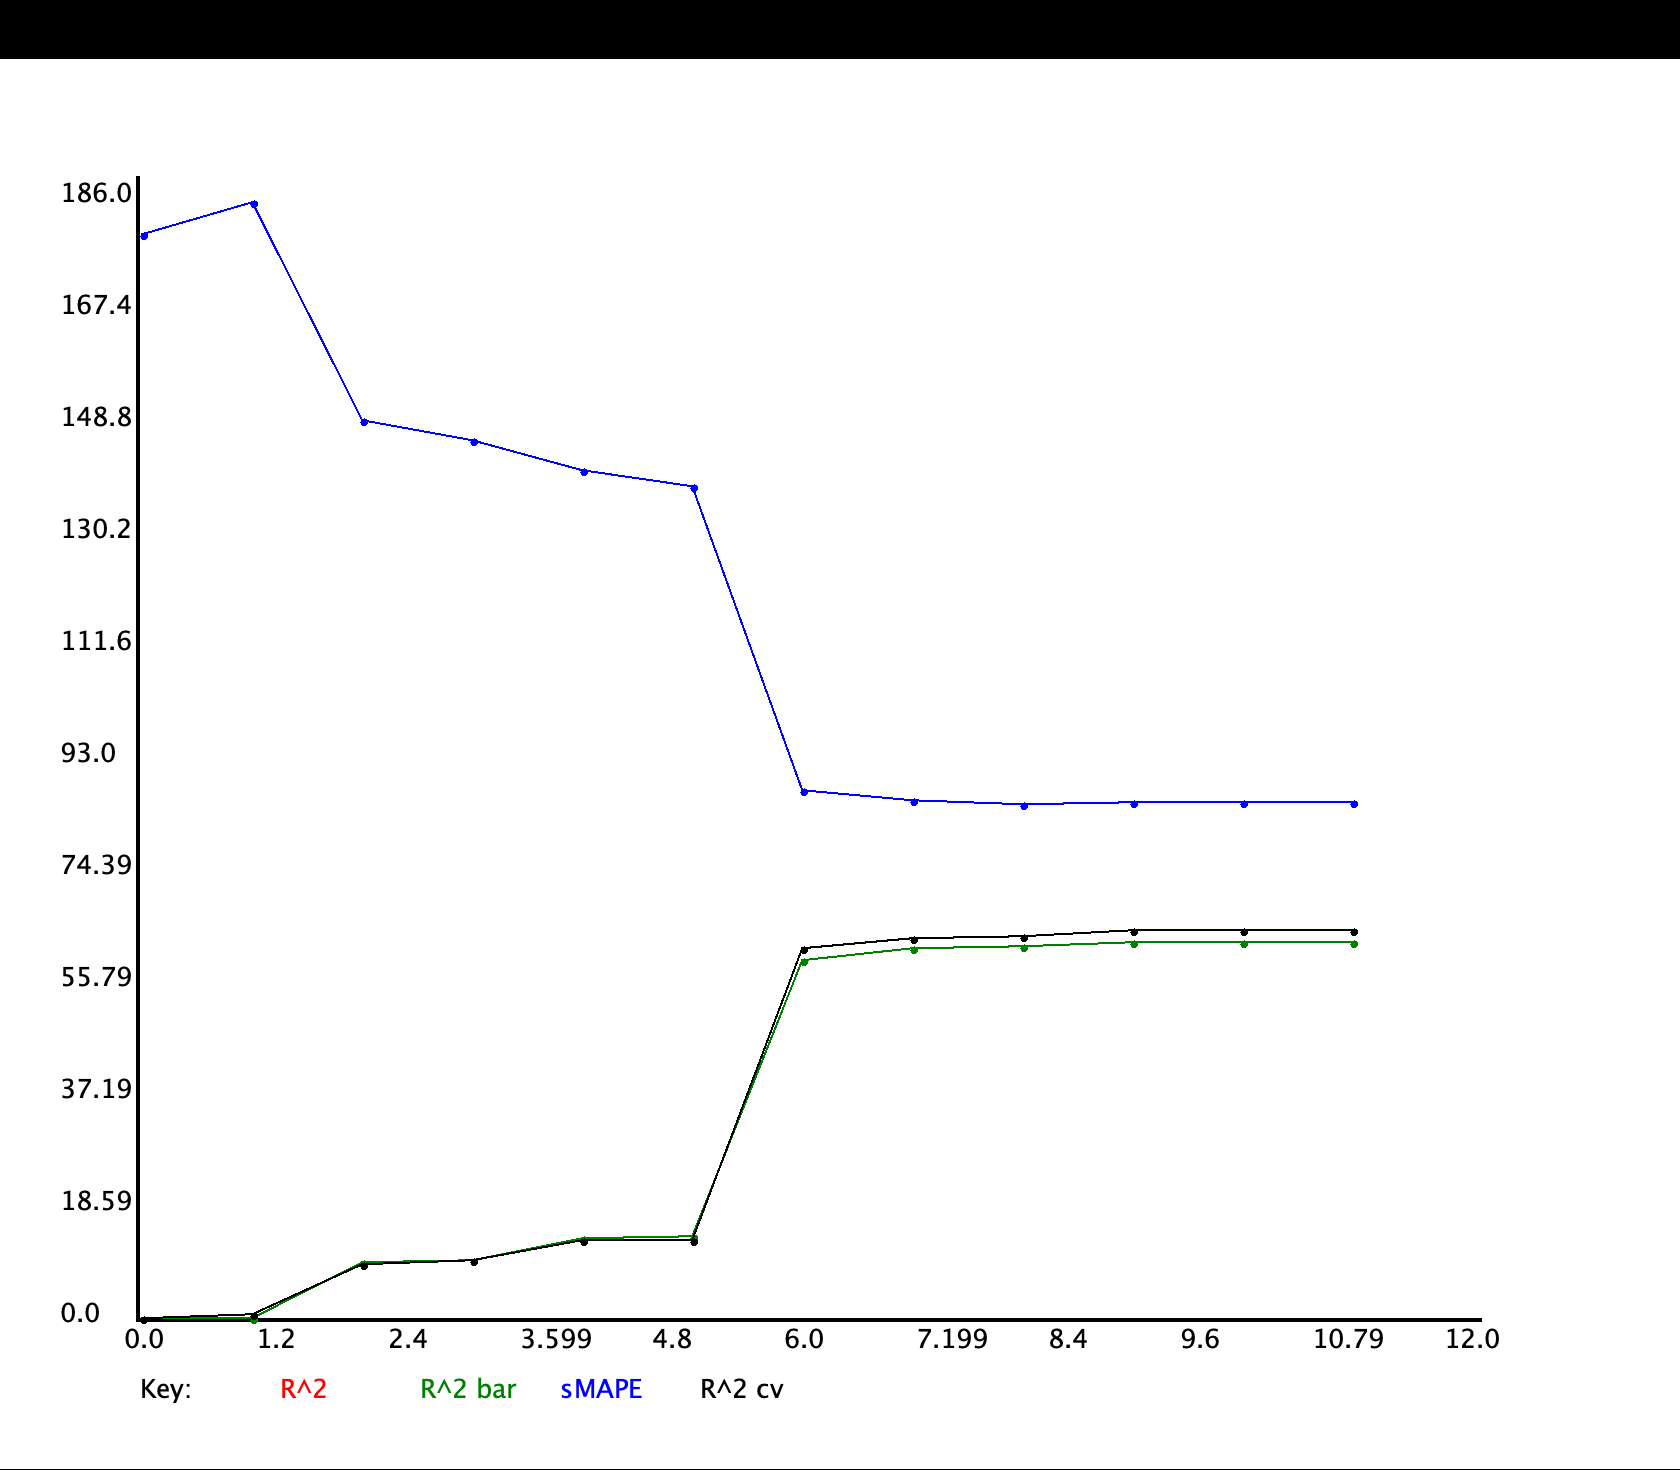
\includegraphics[width=\textwidth]{../House_Prices_Scalation_Plots/Scalation_Ridge_rSq_Forward.png}
     \end{subfigure}
     \hfill
     \begin{subfigure}[b]{0.4\textwidth}
         \centering
         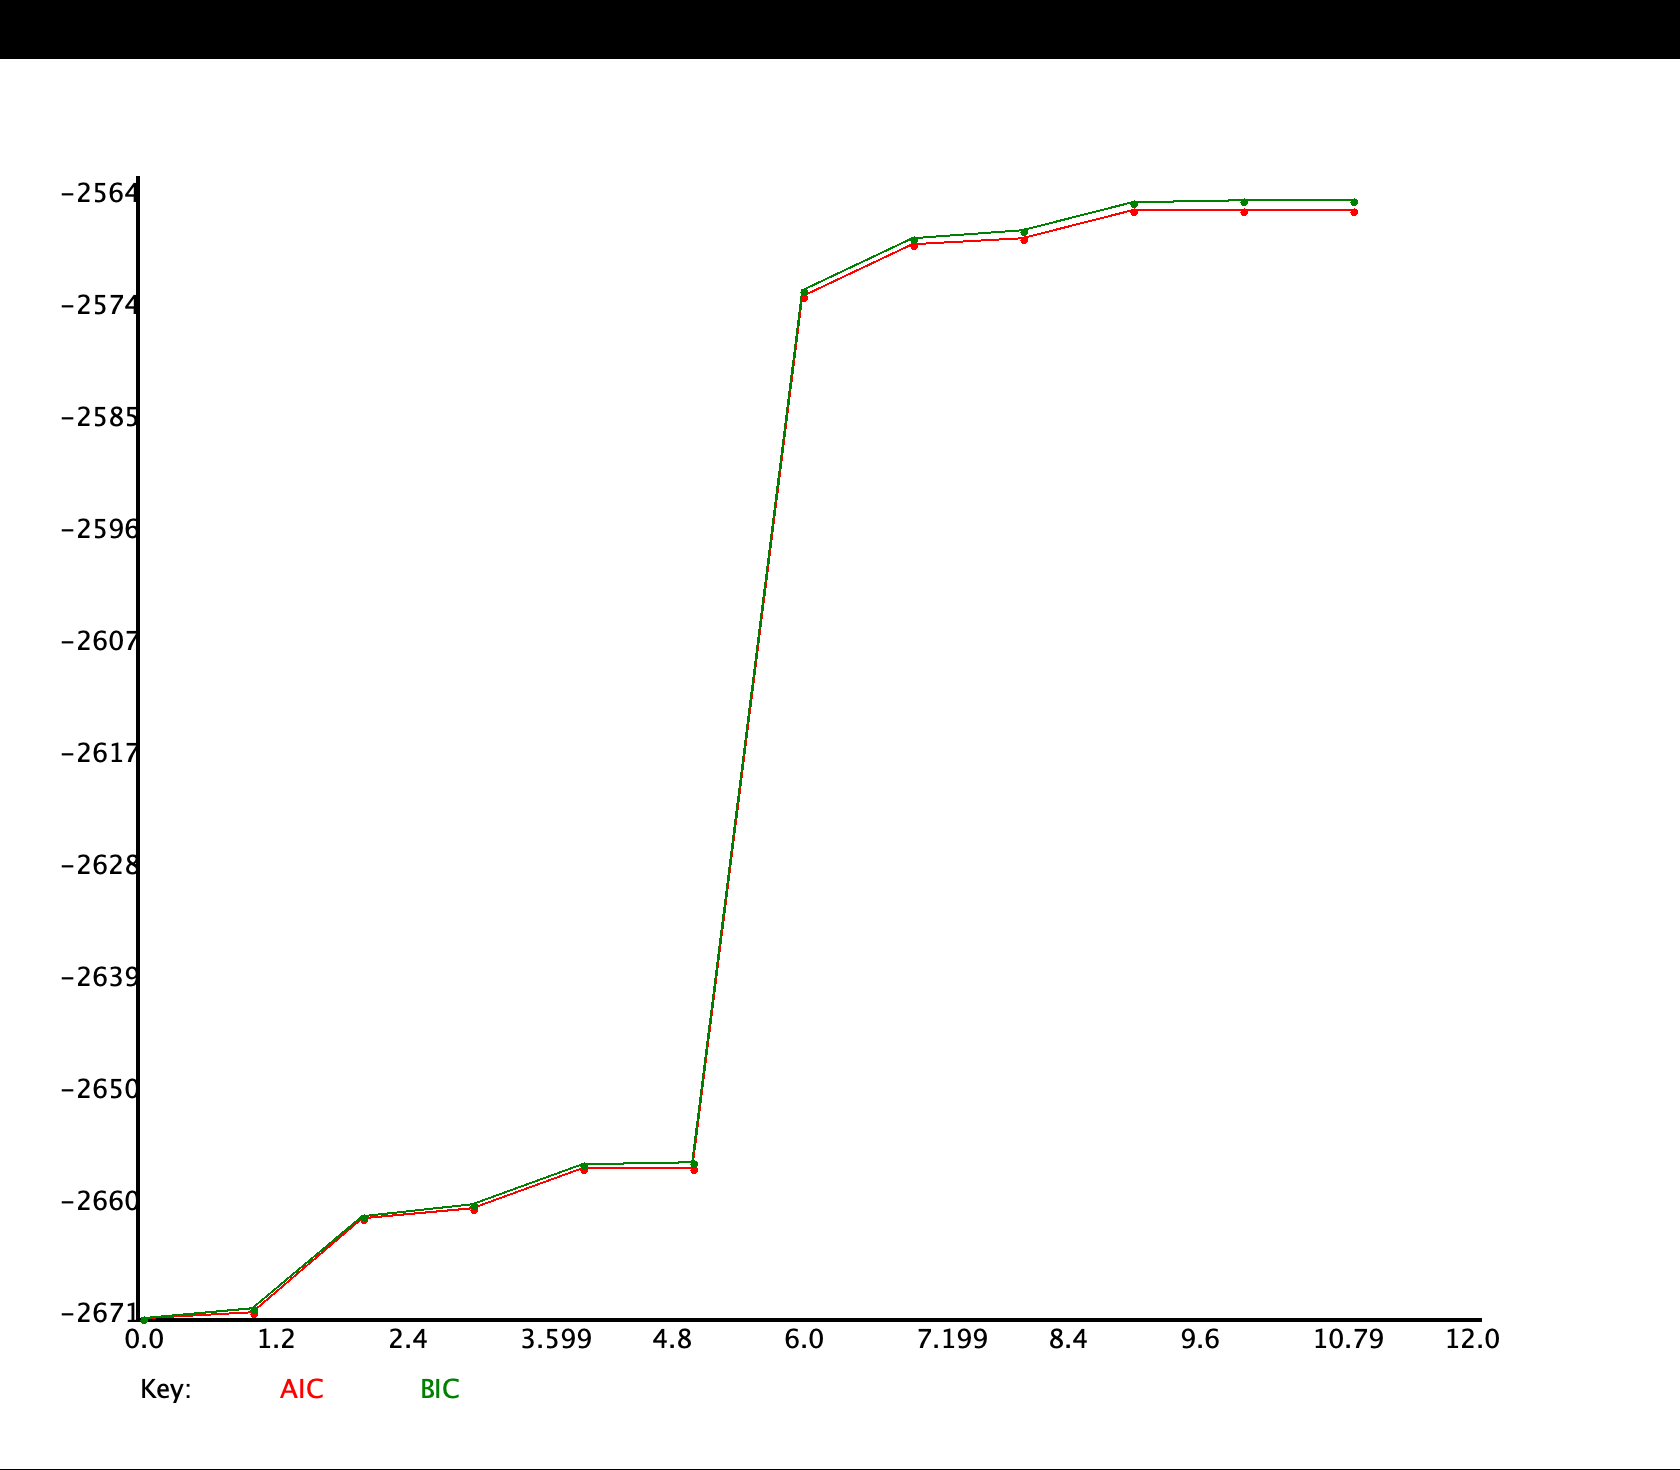
\includegraphics[width=\textwidth]{../House_Prices_Scalation_Plots/Scalation_Ridge_AIC_BIC_Forward.png}
     \end{subfigure}

     \vspace{10pt} % Add some vertical spacing between rows

     % Second Row
     \begin{subfigure}[b]{0.49\textwidth}
         \centering
         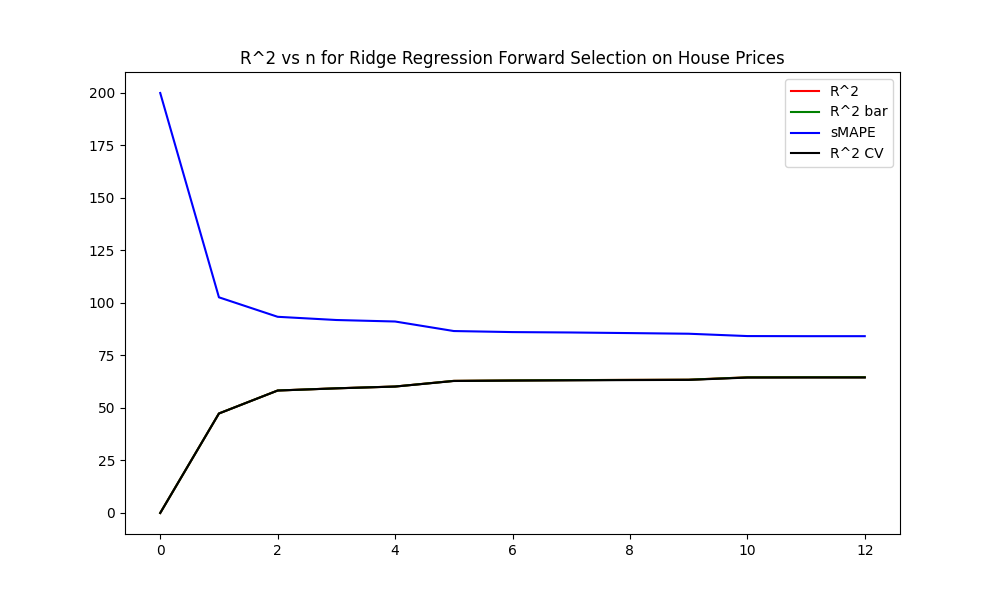
\includegraphics[width=\textwidth]{../House_Prices_Statsmodels_Plots/Statsmodels_Ridge_rSq_Forward.png}
     \end{subfigure}
     \hfill
     \begin{subfigure}[b]{0.49\textwidth}
         \centering
         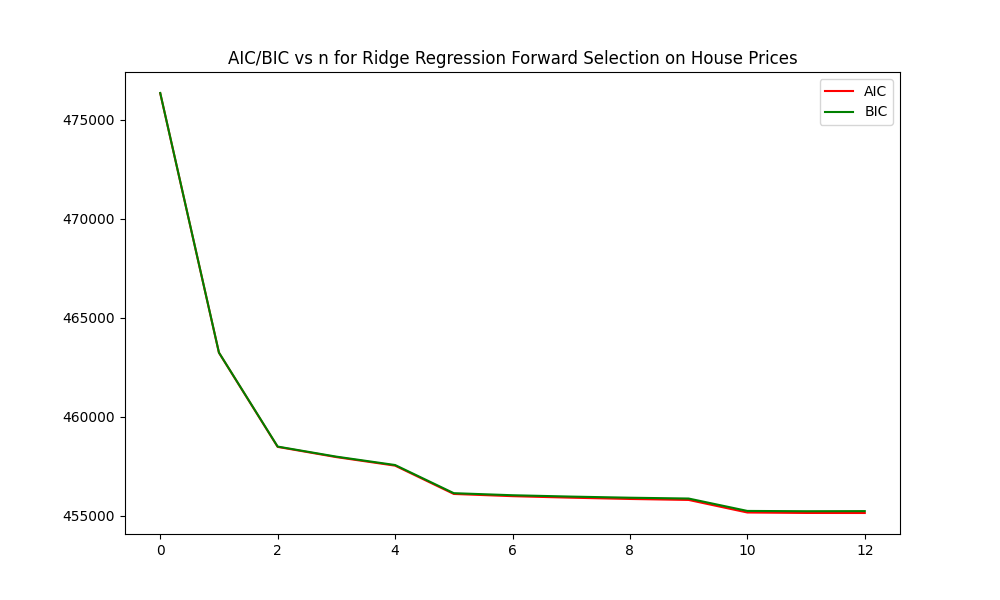
\includegraphics[width=\textwidth]{../House_Prices_Statsmodels_Plots/Statsmodels_Ridge_AIC_BIC_Forward.png}
     \end{subfigure}
     
     \caption{California House Prices Ridge Regression Forward Selection Quality of Fit Metrics\\ Top Left: Scalation $R^2$, Top Right: Scalation AIC/BIC\\ Bottom Left: Statsmodels $R^2$, Bottom Right: Statsmodels AIC/BIC}
     \label{fig:California House Prices Ridge Regression Forward Selection Quality of Fit Metrics}
\end{figure}

Scalation Backward Elimination Reversed: longitude, latitude, median income, total bedrooms, population, housing median age, ocean proximity ISLAND, ocean proximity INLAND, total rooms, households, ocean proximity NEAR BAY, ocean proximity NEAR OCEAN

Statsmodels Backward Elimination Reversed: Null, median income, latitude, longitude, total bedrooms, population, housing median age, ocean proximity INLAND, total rooms, households, ocean proximity ISLAND, ocean proximity NEAR OCEAN, ocean proximity NEAR BAY

\begin{figure}[H]
     \centering
     \captionsetup{justification=centering}
     % First Row
     \begin{subfigure}[b]{0.4\textwidth}
         \centering
         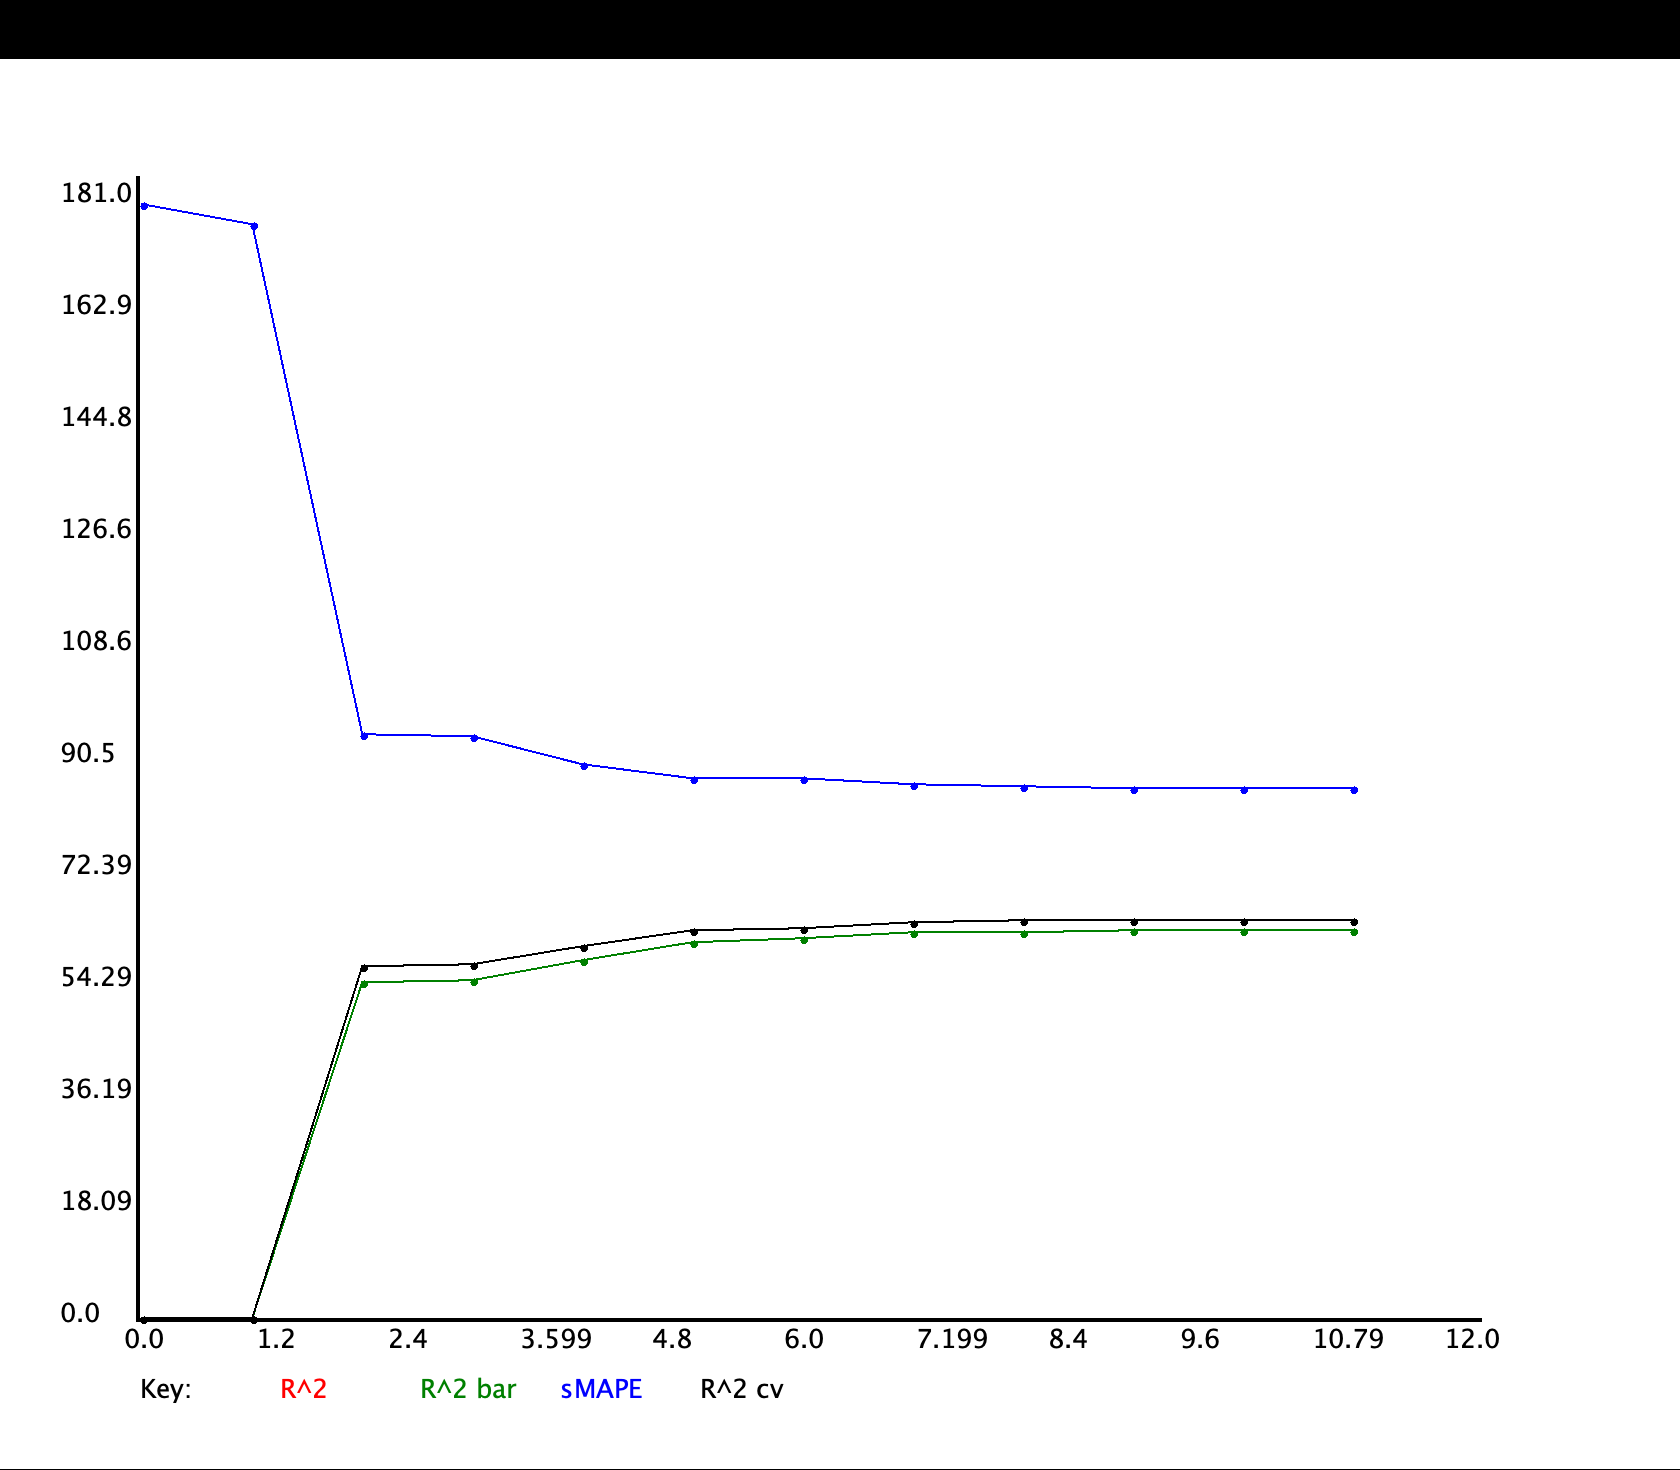
\includegraphics[width=\textwidth]{../House_Prices_Scalation_Plots/Scalation_Ridge_rSq_Backward.png}
     \end{subfigure}
     \hfill
     \begin{subfigure}[b]{0.4\textwidth}
         \centering
         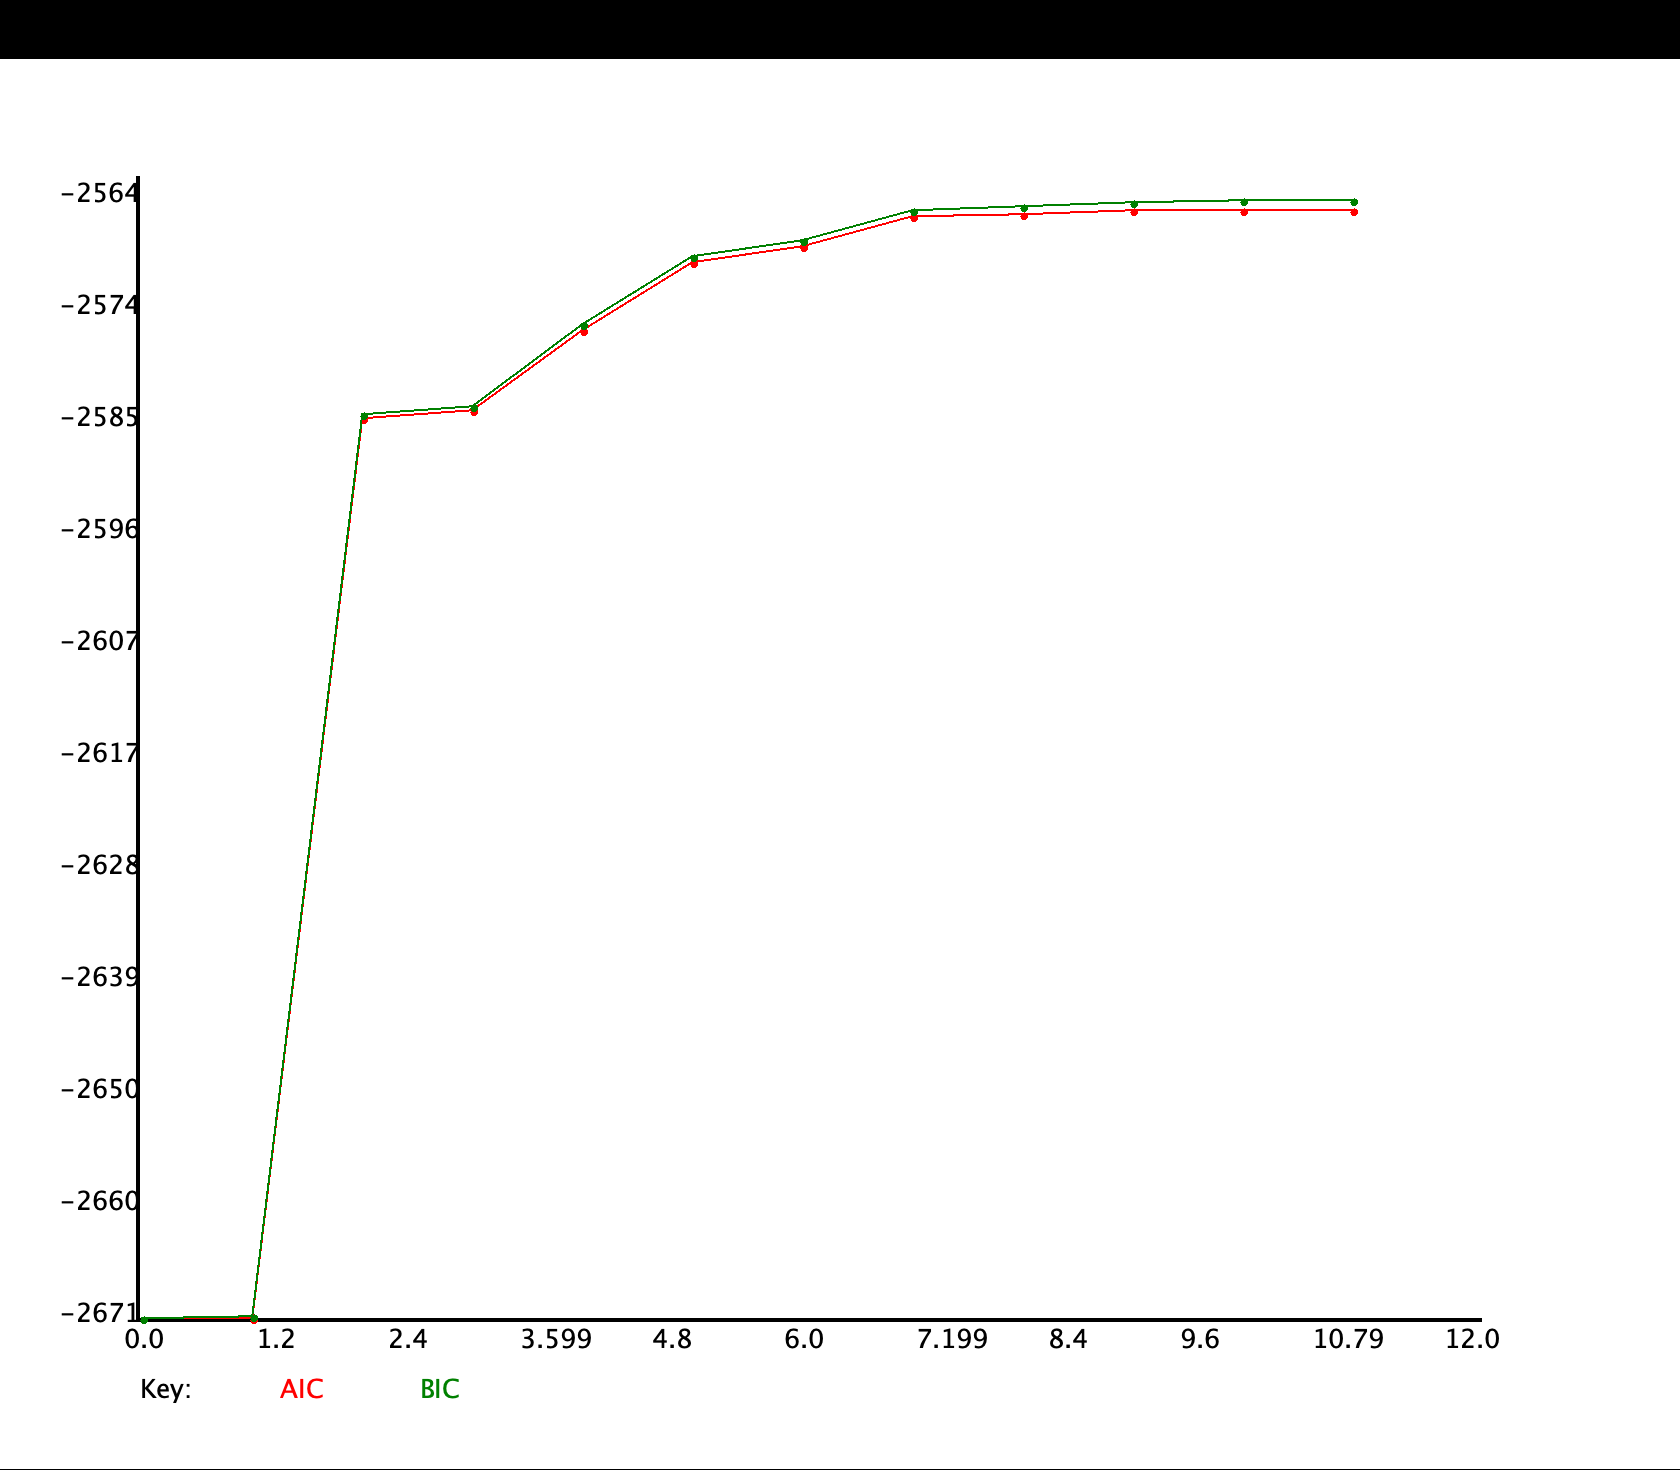
\includegraphics[width=\textwidth]{../House_Prices_Scalation_Plots/Scalation_Ridge_AIC_BIC_Backward.png}
     \end{subfigure}

     \vspace{10pt} % Add some vertical spacing between rows

     % Second Row
     \begin{subfigure}[b]{0.49\textwidth}
         \centering
         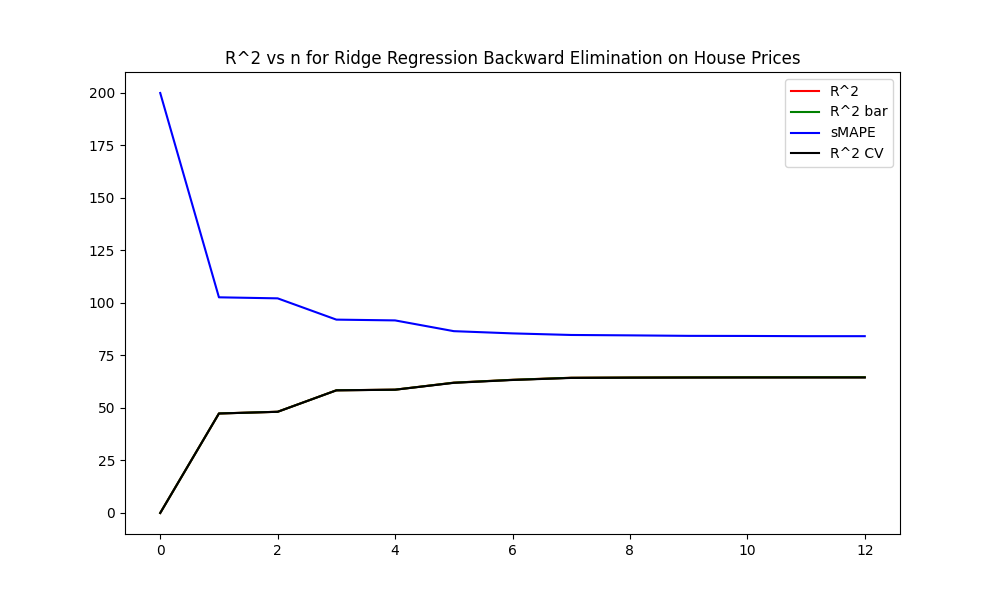
\includegraphics[width=\textwidth]{../House_Prices_Statsmodels_Plots/Statsmodels_Ridge_rSq_Backward.png}
     \end{subfigure}
     \hfill
     \begin{subfigure}[b]{0.49\textwidth}
         \centering
         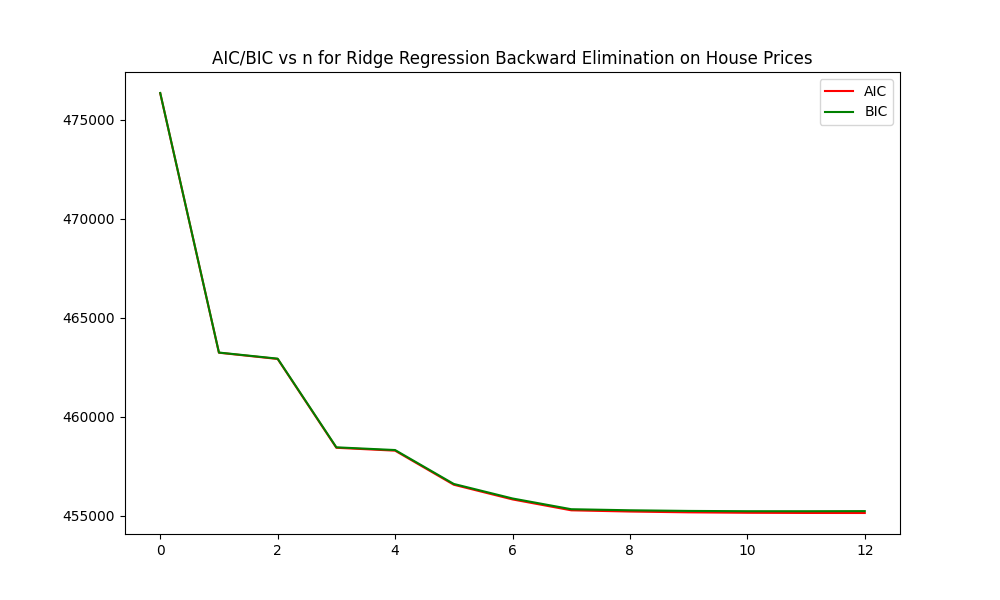
\includegraphics[width=\textwidth]{../House_Prices_Statsmodels_Plots/Statsmodels_Ridge_AIC_BIC_Backward.png}
     \end{subfigure}
     
     \caption{California House Prices Ridge Regression Reversed Backward Elimination Quality of Fit Metrics\\ Top Left: Scalation $R^2$, Top Right: Scalation AIC/BIC\\ Bottom Left: Statsmodels $R^2$, Bottom Right: Statsmodels AIC/BIC}
     \label{fig:California House Prices Ridge Regression Reversed Backward Elimination Quality of Fit Metrics}
\end{figure}

Scalation Stepwise Selection: longitude, total rooms, population, total bedrooms, households, latitude, median income, housing median age, ocean proximity INLAND, ocean proximity ISLAND, ocean proximity NEAR BAY

Statsmodels Stepwise Selection: Null, median income, ocean proximity INLAND, housing median age, total bedrooms, population, households, total rooms, ocean proximity NEAR OCEAN, longitude, latitude, ocean proximity ISLAND, ocean proximity NEAR BAY

\begin{figure}[H]
     \centering
     \captionsetup{justification=centering}
     % First Row
     \begin{subfigure}[b]{0.4\textwidth}
         \centering
         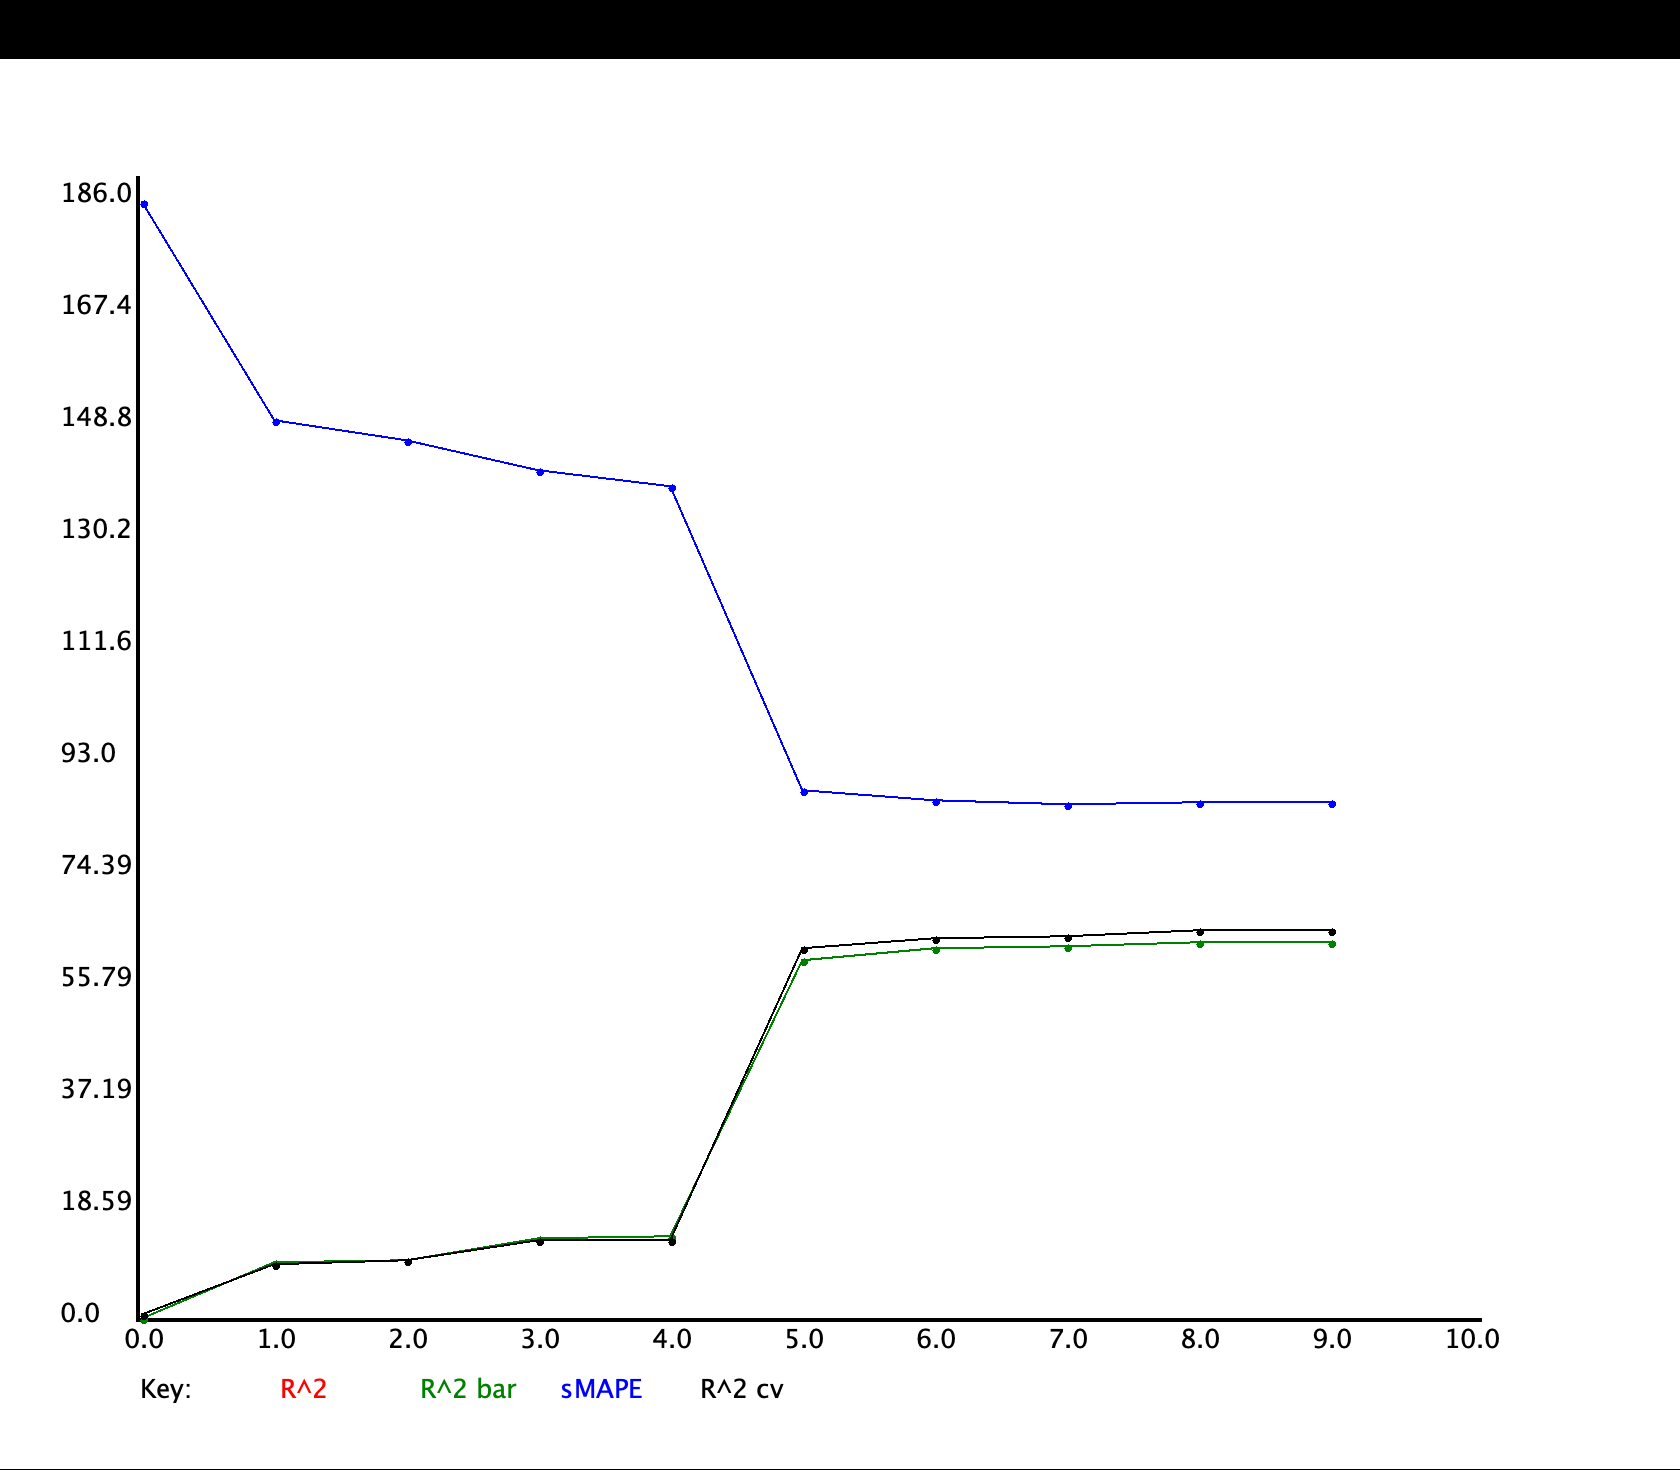
\includegraphics[width=\textwidth]{../House_Prices_Scalation_Plots/Scalation_Ridge_rSq_Stepwise.png}
     \end{subfigure}
     \hfill
     \begin{subfigure}[b]{0.4\textwidth}
         \centering
         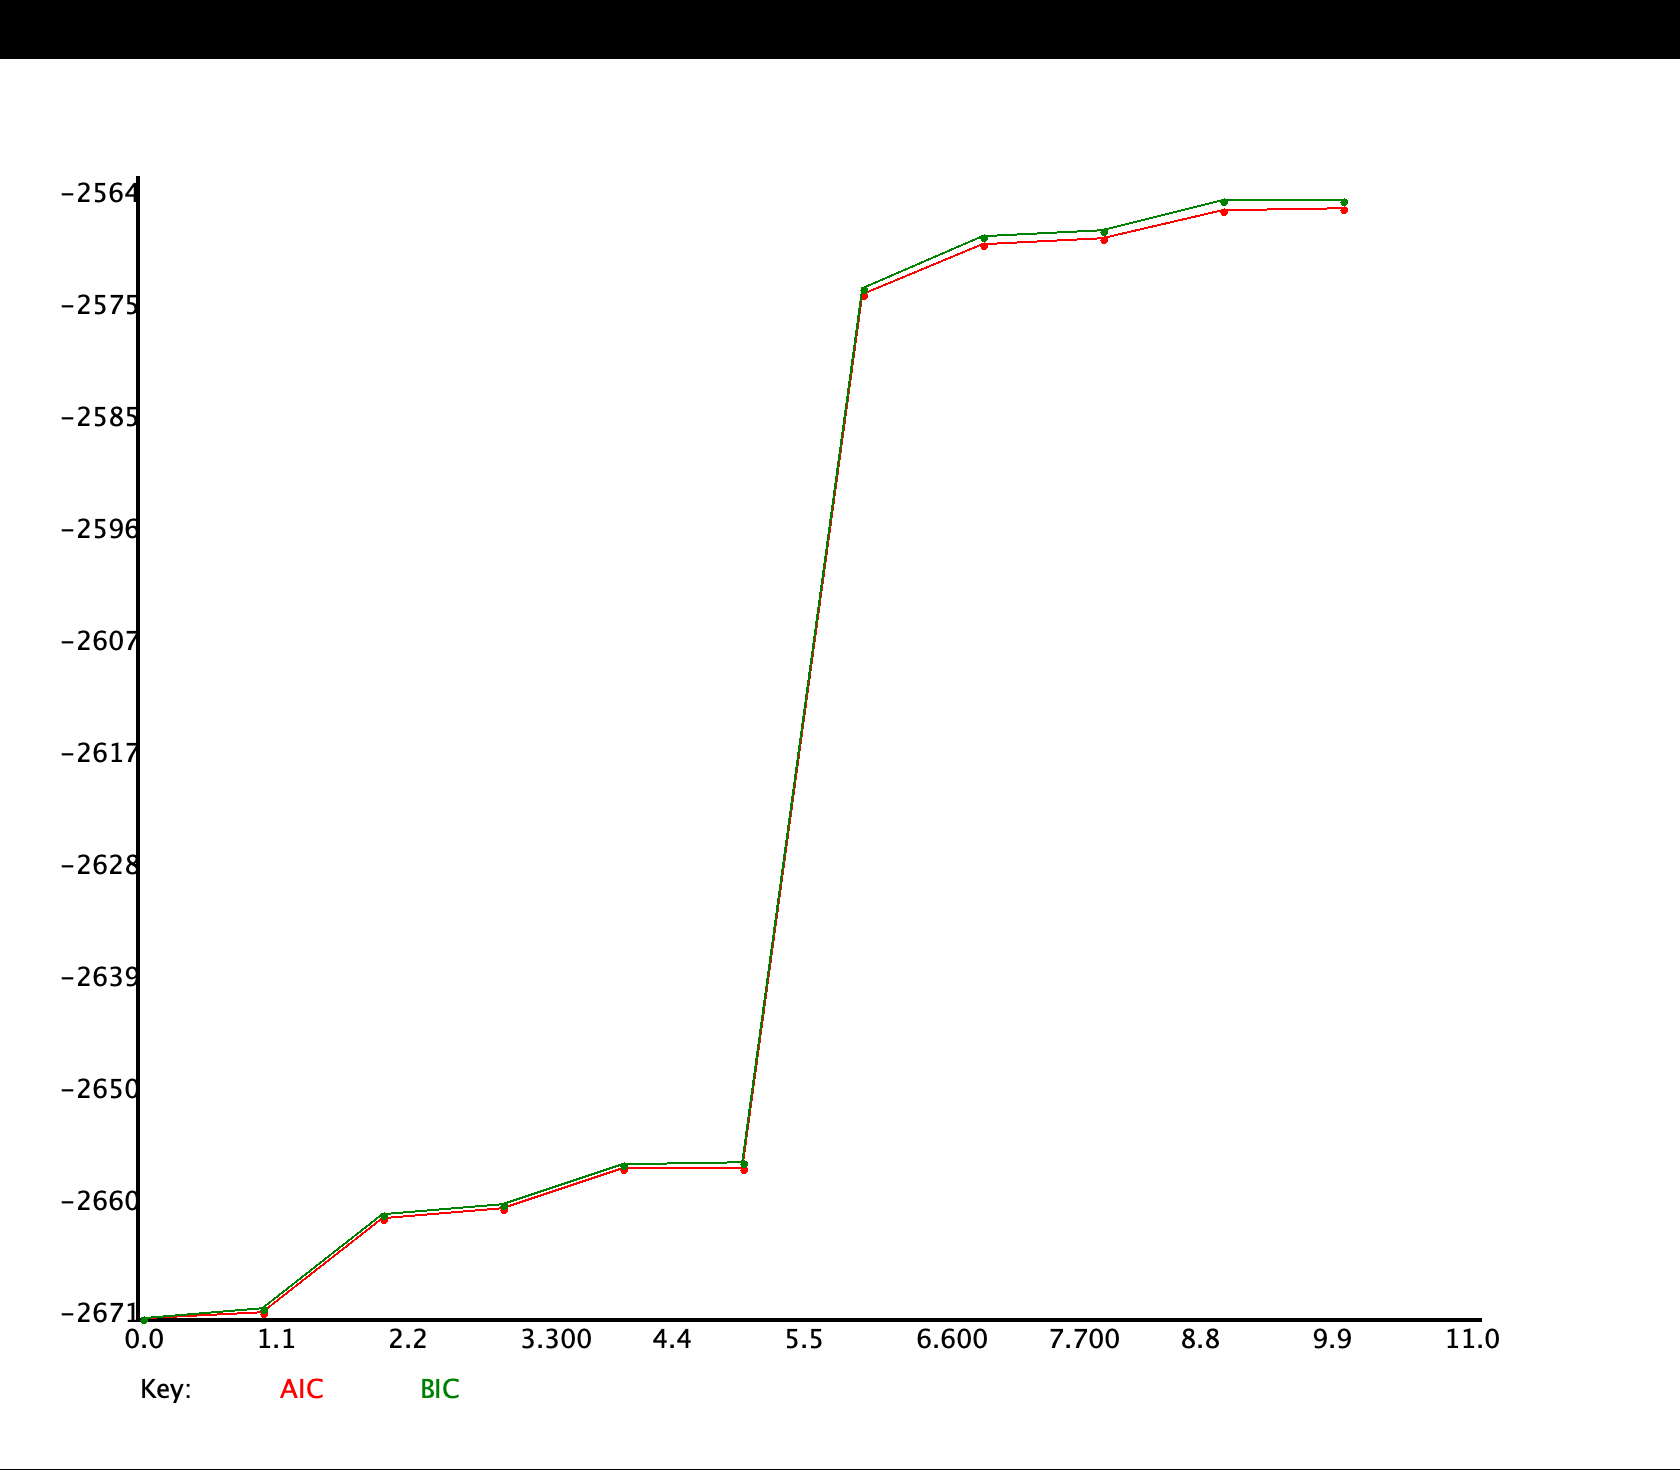
\includegraphics[width=\textwidth]{../House_Prices_Scalation_Plots/Scalation_Ridge_AIC_BIC_Stepwise.png}
     \end{subfigure}

     \vspace{10pt} % Add some vertical spacing between rows

     % Second Row
     \begin{subfigure}[b]{0.49\textwidth}
         \centering
         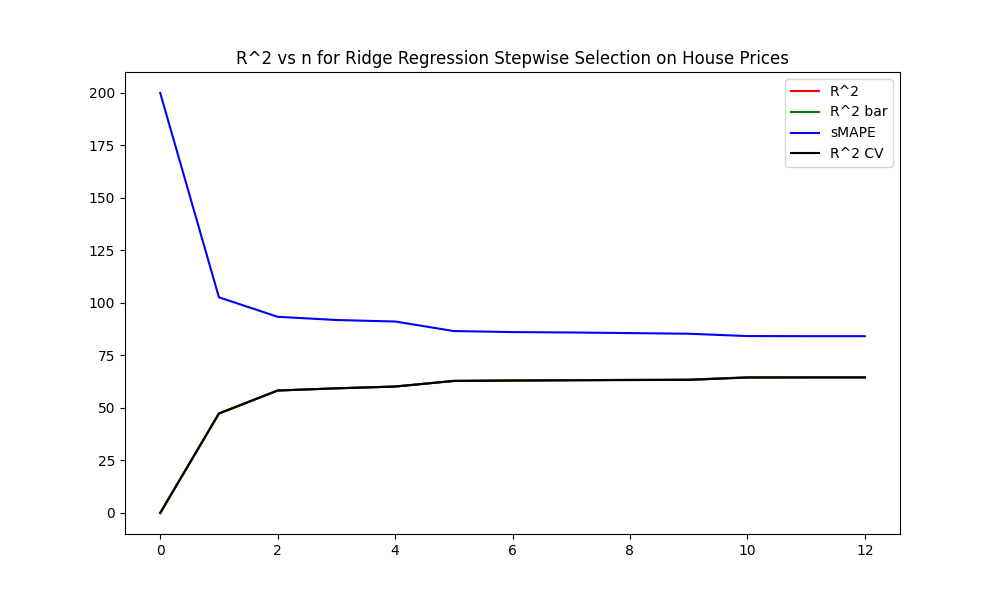
\includegraphics[width=\textwidth]{../House_Prices_Statsmodels_Plots/Statsmodels_Ridge_rSq_Stepwise.png}
     \end{subfigure}
     \hfill
     \begin{subfigure}[b]{0.49\textwidth}
         \centering
         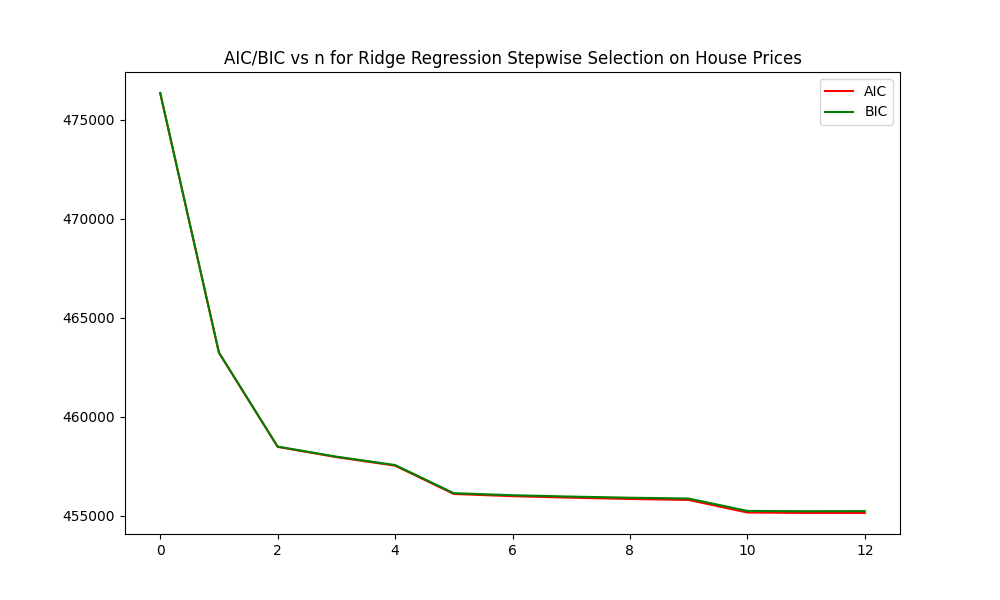
\includegraphics[width=\textwidth]{../House_Prices_Statsmodels_Plots/Statsmodels_Ridge_AIC_BIC_Stepwise.png}
     \end{subfigure}
     
     \caption{California House Prices Ridge Regression Stepwise Selection Quality of Fit Metrics\\ Top Left: Scalation $R^2$, Top Right: Scalation AIC/BIC\\ Bottom Left: Statsmodels $R^2$, Bottom Right: Statsmodels AIC/BIC}
     \label{fig:California House Prices Ridge Regression Stepwise Selection Quality of Fit Metrics}
\end{figure}

\subsection{Lasso Regression}

\subsubsection{Quality of Fit}

Scalation California House Prices Lasso Lambda Used: $0.00001$

\noindent Scalation California House Prices Lasso Selected Features: longitude, latitude, housing median age, total bedrooms, households, median income, ocean proximity INLAND, ocean proximity ISLAND, ocean proximity NEAR BAY, ocean proximity NEAR OCEAN

\noindent Statsmodels California House Prices Lasso alpha Used: $0.000000001$ 1e-09

\noindent Statsmodels California House Prices Lasso Selected Features: longitude, latitude, housing median age, total rooms, total bedrooms, population, households, median income, ocean proximity INLAND, ocean proximity ISLAND, ocean proximity NEAR BAY, ocean proximity NEAR OCEAN

\begin{table}[H]
\centering
\caption{Scalation - California House Prices Lasso Regression}
\label{tab:Scalation - House Prices Lasso Regression}
\begin{tabular}{|c|c|c|} \hline 
Metric & In-Sample & 80-20 Split \\ \hline \hline 
rSq &-0.00968812 &      0.0156508 \\ \hline 
rSqBar &-0.0102320 &    0.0151206 \\ \hline 
sst &2.72264e+14 &      5.31945e+13 \\ \hline 
sse &2.74902e+14 &      5.23620e+13 \\ \hline 
sde &87969.4 &  85496.5 \\ \hline 
mse0 &1.34538e+10 &     1.28150e+10 \\ \hline 
rmse &115991 &  113203 \\ \hline 
mae &95289.0 &  93495.5 \\ \hline 
smape &124.674 &        123.972 \\ \hline 
m &20433.0 &    4086.00 \\ \hline 
dfr &11.0000 &  11.0000 \\ \hline 
df &20421.0 &   20421.0 \\ \hline 
fStat &-17.8130 &       29.5169 \\ \hline 
aic &-269139 &  -53714.4 \\ \hline 
bic &-269044 &  -53638.6 \\ \hline 
\end{tabular}
\end{table}

\begin{table}[H]
\centering
\caption{Statsmodels - California House Prices Lasso Regression}
\label{tab:Statsmodels - House Prices Lasso Regression}
\begin{tabular}{|c|c|c|}\hline
Metric & In-Sample & 80-20 Split \\ \hline \hline
rSq & 0.6463 & 0.6530 \\ \hline
rSqBar & 0.6461 & 0.6520 \\ \hline
sst & 272264434648930.1562 & 54723646809444.8438 \\ \hline
sse & 96294625051999.0625 & 18991156140776.2188 \\ \hline
sde & 68669.2842 & 68267.1694 \\ \hline
mse0 & 4712701270.1022 & 4646722813.9898 \\ \hline
rmse & 68649.1170 & 68166.8748 \\ \hline
mae & 49748.0842 & 49939.2025 \\ \hline
smape & 84.1387 & 84.5056 \\ \hline
m & 20433.0000 & 4087.0000 \\ \hline
dfr & 12.0000 & 12.0000 \\ \hline
df & 20421.0000 & 4075.0000 \\ \hline
fStat & 3109.7958 & 638.9373 \\ \hline
aic & 455138.9792 & 90998.2824 \\ \hline
bic & 455234.0781 & 91074.0692 \\ \hline
\end{tabular}
\end{table}

\begin{table}[H]
\centering
\caption{Scalation - California House Prices Lasso Regression CV}
\label{tab:Scalation - California House Prices Lasso Regression CV}
\begin{tabular}{|c|c|c|c|c|c|}\hline
Metric & num folds & min & max & mean & stdev \\ \hline \hline
rSq & 5 & -0.019 & 0.614 & 0.132 & 0.270 \\ \hline
rSqBar & 5 & -0.020 & 0.614 & 0.132 & 0.270 \\ \hline
sst & 5 & 53194492241132.950 & 57310203956797.310 & 54411355017051.120 & 1675890609057.038 \\ \hline
sse & 5 & 20948489055322.040 & 55182245244389.914 & 47221248820746.540 & 14739866714894.100 \\ \hline
sde & 5 & 70011.021 & 89290.509 & 83854.383 & 7918.193 \\ \hline
mse0 & 5 & 5126894041.929 & 13505199521.388 & 11556840142.131 & 3607407419.210 \\ \hline
rmse & 5 & 71602.333 & 116211.873 & 106103.006 & 19332.367 \\ \hline
mae & 5 & 53701.805 & 95987.765 & 86357.446 & 18282.622 \\ \hline
smape & 5 & 90.384 & 125.082 & 117.628 & 15.241 \\ \hline
m & 5 & 4086.000 & 4086.000 & 4086.000 & 0.000 \\ \hline
dfr & 5 & 11.000 & 11.000 & 11.000 & 0.000 \\ \hline
df & 5 & 20421.000 & 20421.000 & 20421.000 & 0.000 \\ \hline
fStat & 5 & -34.748 & 2956.190 & 609.148 & 1312.583 \\ \hline
aic & 5 & -53907.380 & -51565.126 & -53362.693 & 1008.493 \\ \hline
bic & 5 & -53831.596 & -51489.342 & -53286.909 & 1008.493 \\ \hline
\end{tabular}
\end{table}

\begin{table}[H]
\centering
\caption{Statsmodels - California House Prices Lasso Regression CV}
\label{tab:Statsmodels - House Prices Lasso Regression CV}
\begin{tabular}{|c|c|c|c|c|c|}\hline
Metric & num folds & min & max & mean & stdev \\ \hline \hline
rSq & 5 & 0.6192 & 0.6547 & 0.6449 & 0.0131 \\ \hline
rSqBar & 5 & 0.6182 & 0.6537 & 0.6440 & 0.0131 \\ \hline
sst & 5 & 53541750406767.3438 & 54912923487891.5859 & 54447676367709.7031 & 499826929365.4294 \\ \hline
sse & 5 & 18963981588141.3672 & 20388319526653.5547 & 19326526964540.0859 & 544213618515.1556 \\ \hline
sde & 5 & 68218.3100 & 70742.4674 & 68864.0168 & 963.1592 \\ \hline
mse0 & 5 & 4640073792.0581 & 4989799198.8873 & 4729252460.6946 & 133496906.6999 \\ \hline
rmse & 5 & 68118.0871 & 70638.5107 & 68762.8353 & 961.7372 \\ \hline
mae & 5 & 49044.8661 & 50417.1856 & 49797.1535 & 445.7714 \\ \hline
smape & 5 & 82.6551 & 85.5011 & 84.1659 & 0.9273 \\ \hline
m & 5 & 4086.0000 & 4087.0000 & 4086.6000 & 0.4899 \\ \hline
dfr & 5 & 12.0000 & 12.0000 & 12.0000 & 0.0000 \\ \hline
df & 5 & 4074.0000 & 4075.0000 & 4074.6000 & 0.4899 \\ \hline
fStat & 5 & 552.0607 & 643.7288 & 617.9881 & 33.6175 \\ \hline
aic & 5 & 90978.3873 & 91267.0829 & 91059.7265 & 107.6353 \\ \hline
bic & 5 & 91054.1712 & 91342.8668 & 91135.5121 & 107.6346 \\ \hline
\end{tabular}
\end{table}

\begin{figure}[H]
     \centering
     \captionsetup{justification=centering}
     % First Row
     \begin{subfigure}[b]{0.4\textwidth}
         \centering
         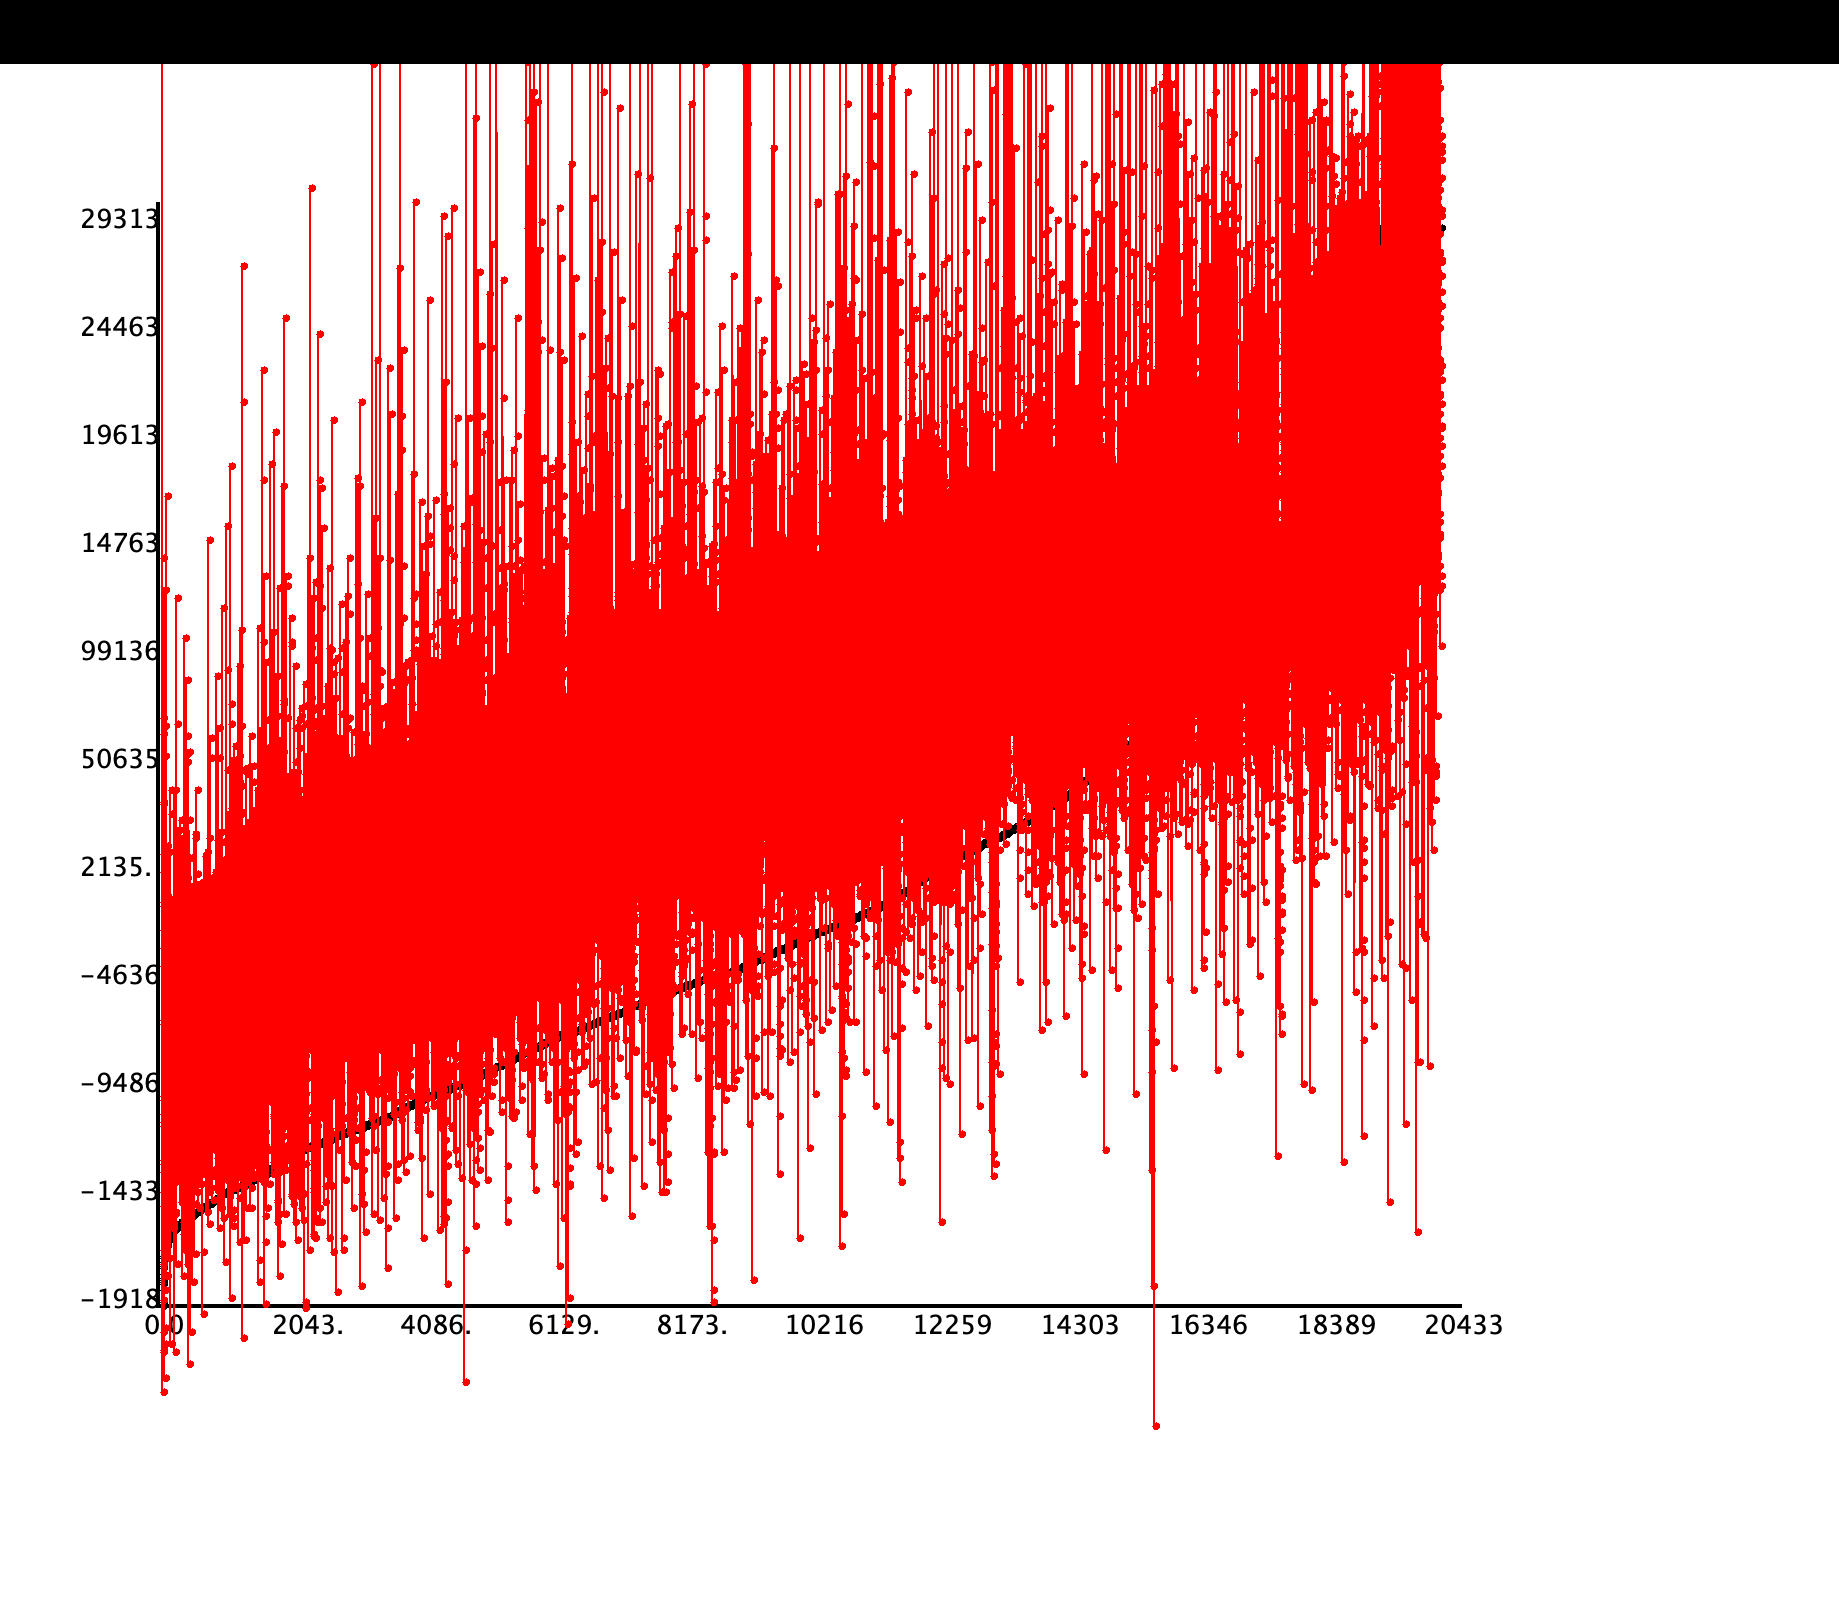
\includegraphics[width=\textwidth]{../House_Prices_Scalation_Plots/Scalation_Lasso_In_Sample.png}
     \end{subfigure}
     \hfill
     \begin{subfigure}[b]{0.4\textwidth}
         \centering
         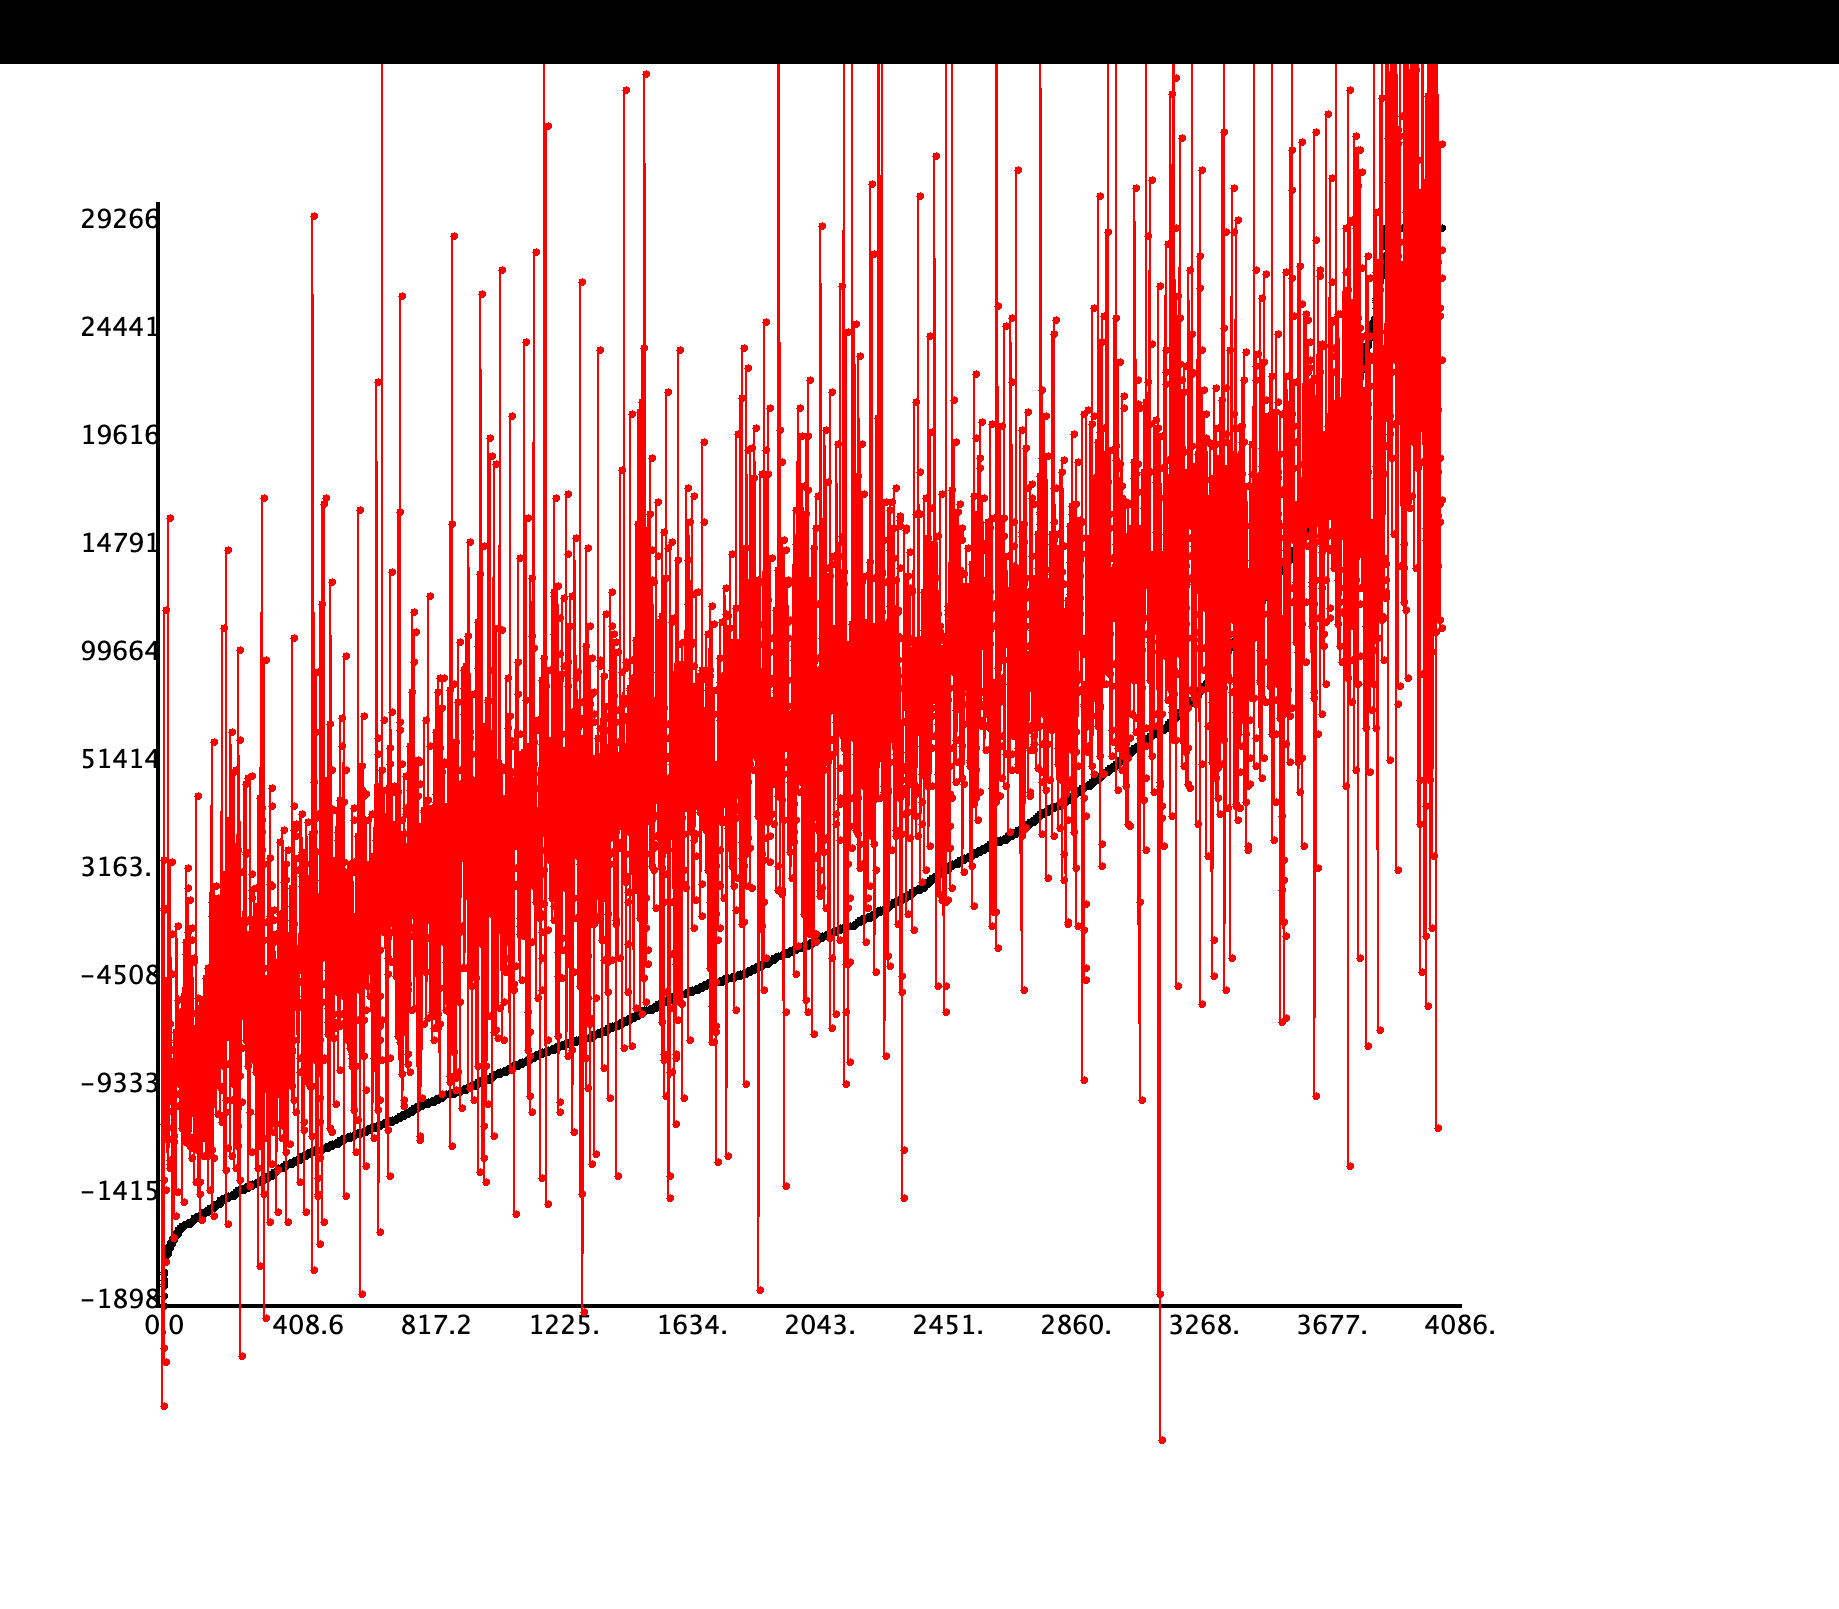
\includegraphics[width=\textwidth]{../House_Prices_Scalation_Plots/Scalation_Lasso_80_20.png}
     \end{subfigure}

     \vspace{10pt} % Add some vertical spacing between rows

     % Second Row
     \begin{subfigure}[b]{0.49\textwidth}
         \centering
         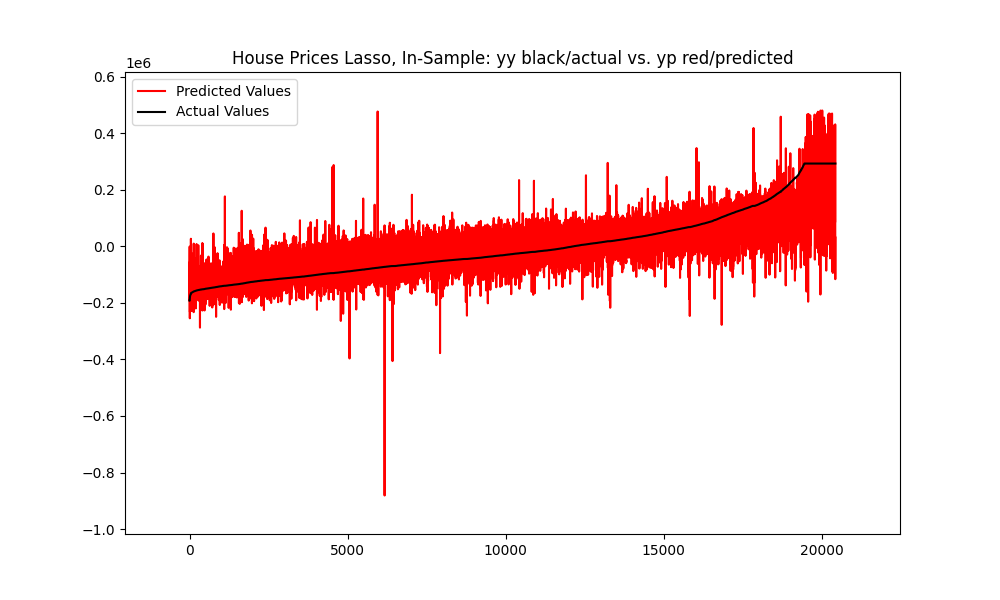
\includegraphics[width=\textwidth]{../House_Prices_Statsmodels_Plots/Statsmodels_Lasso_In_Sample.png}
     \end{subfigure}
     \hfill
     \begin{subfigure}[b]{0.49\textwidth}
         \centering
         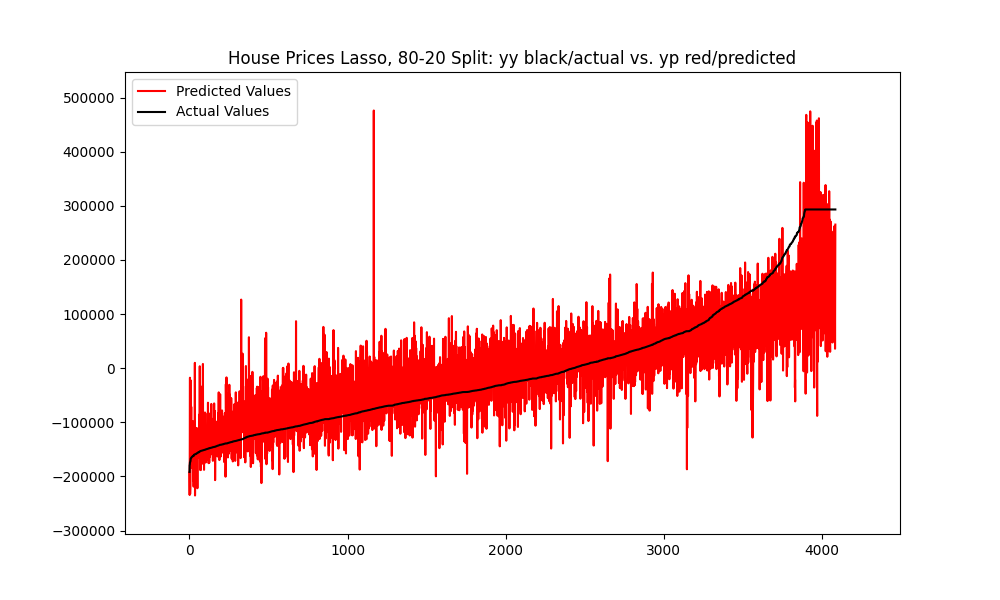
\includegraphics[width=\textwidth]{../House_Prices_Statsmodels_Plots/Statsmodels_Lasso_80_20.png}
     \end{subfigure}
     
     \caption{California House Prices Lasso Regression Plots\\ Top Left: Scalation In-Sample, Top Right: Scalation Out-of-Sample\\ Bottom Left: Statsmodels In-Sample, Bottom Right: Statsmodels Out-of-Sample\\ black: actual y-values, red: predicted y-values}
     \label{fig:California House Prices Lasso Regression Plots}
\end{figure}

\subsubsection{Feature Selection}

Scalation Forward Selection: longitude, total rooms, population, total bedrooms, households, latitude, housing median age, ocean proximity INLAND, ocean proximity NEAR BAY, ocean proximity ISLAND, median income, ocean proximity NEAR OCEAN

Statsmodels Forward Selection: Null, median income, ocean proximity INLAND, housing median age, total bedrooms, population, households, total rooms, ocean proximity NEAR OCEAN, longitude, latitude, ocean proximity ISLAND, ocean proximity NEAR BAY

\begin{figure}[H]
     \centering
     \captionsetup{justification=centering}
     % First Row
     \begin{subfigure}[b]{0.4\textwidth}
         \centering
         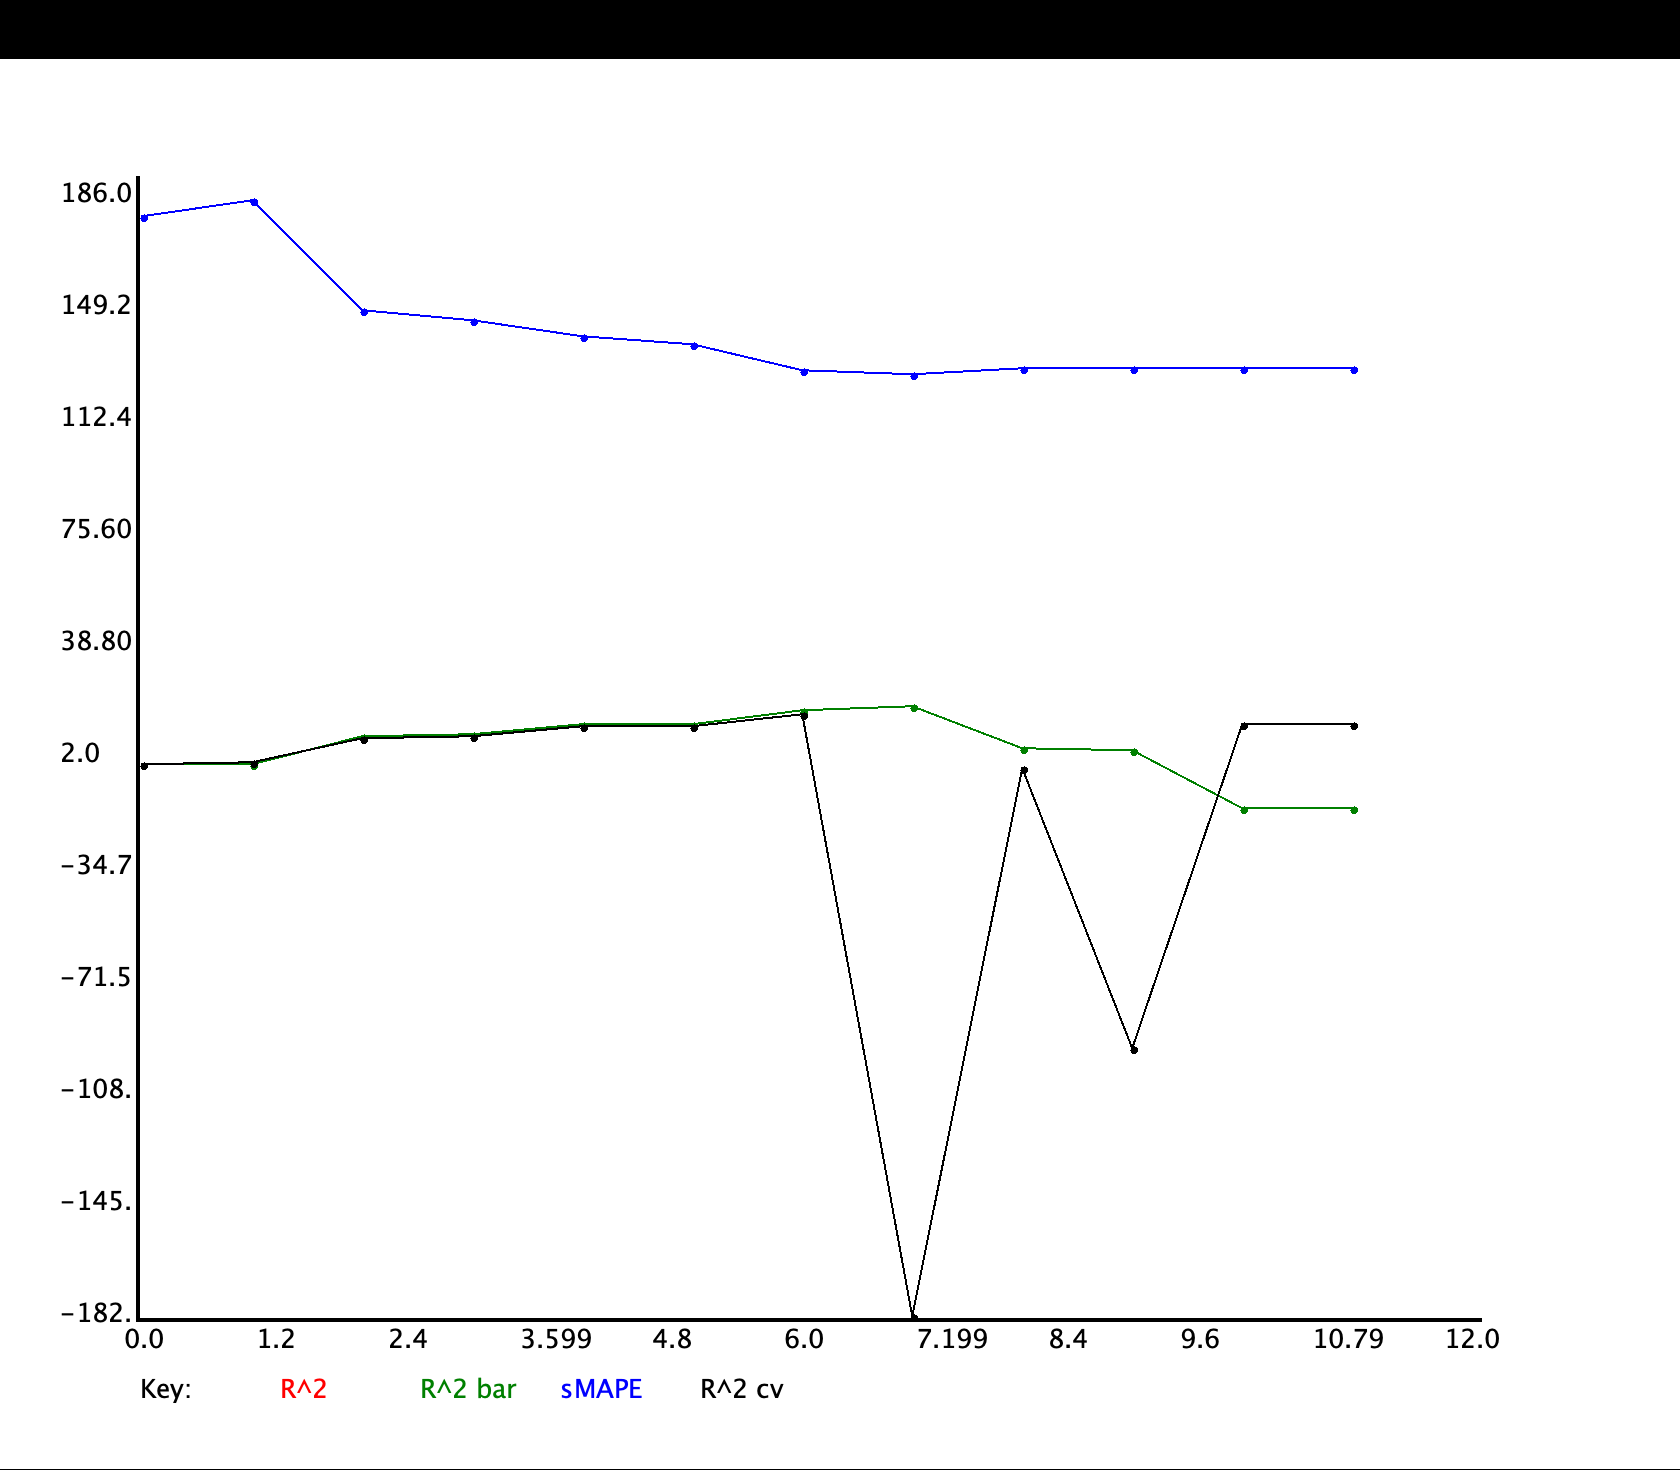
\includegraphics[width=\textwidth]{../House_Prices_Scalation_Plots/Scalation_Lasso_rSq_Forward.png}
     \end{subfigure}
     \hfill
     \begin{subfigure}[b]{0.4\textwidth}
         \centering
         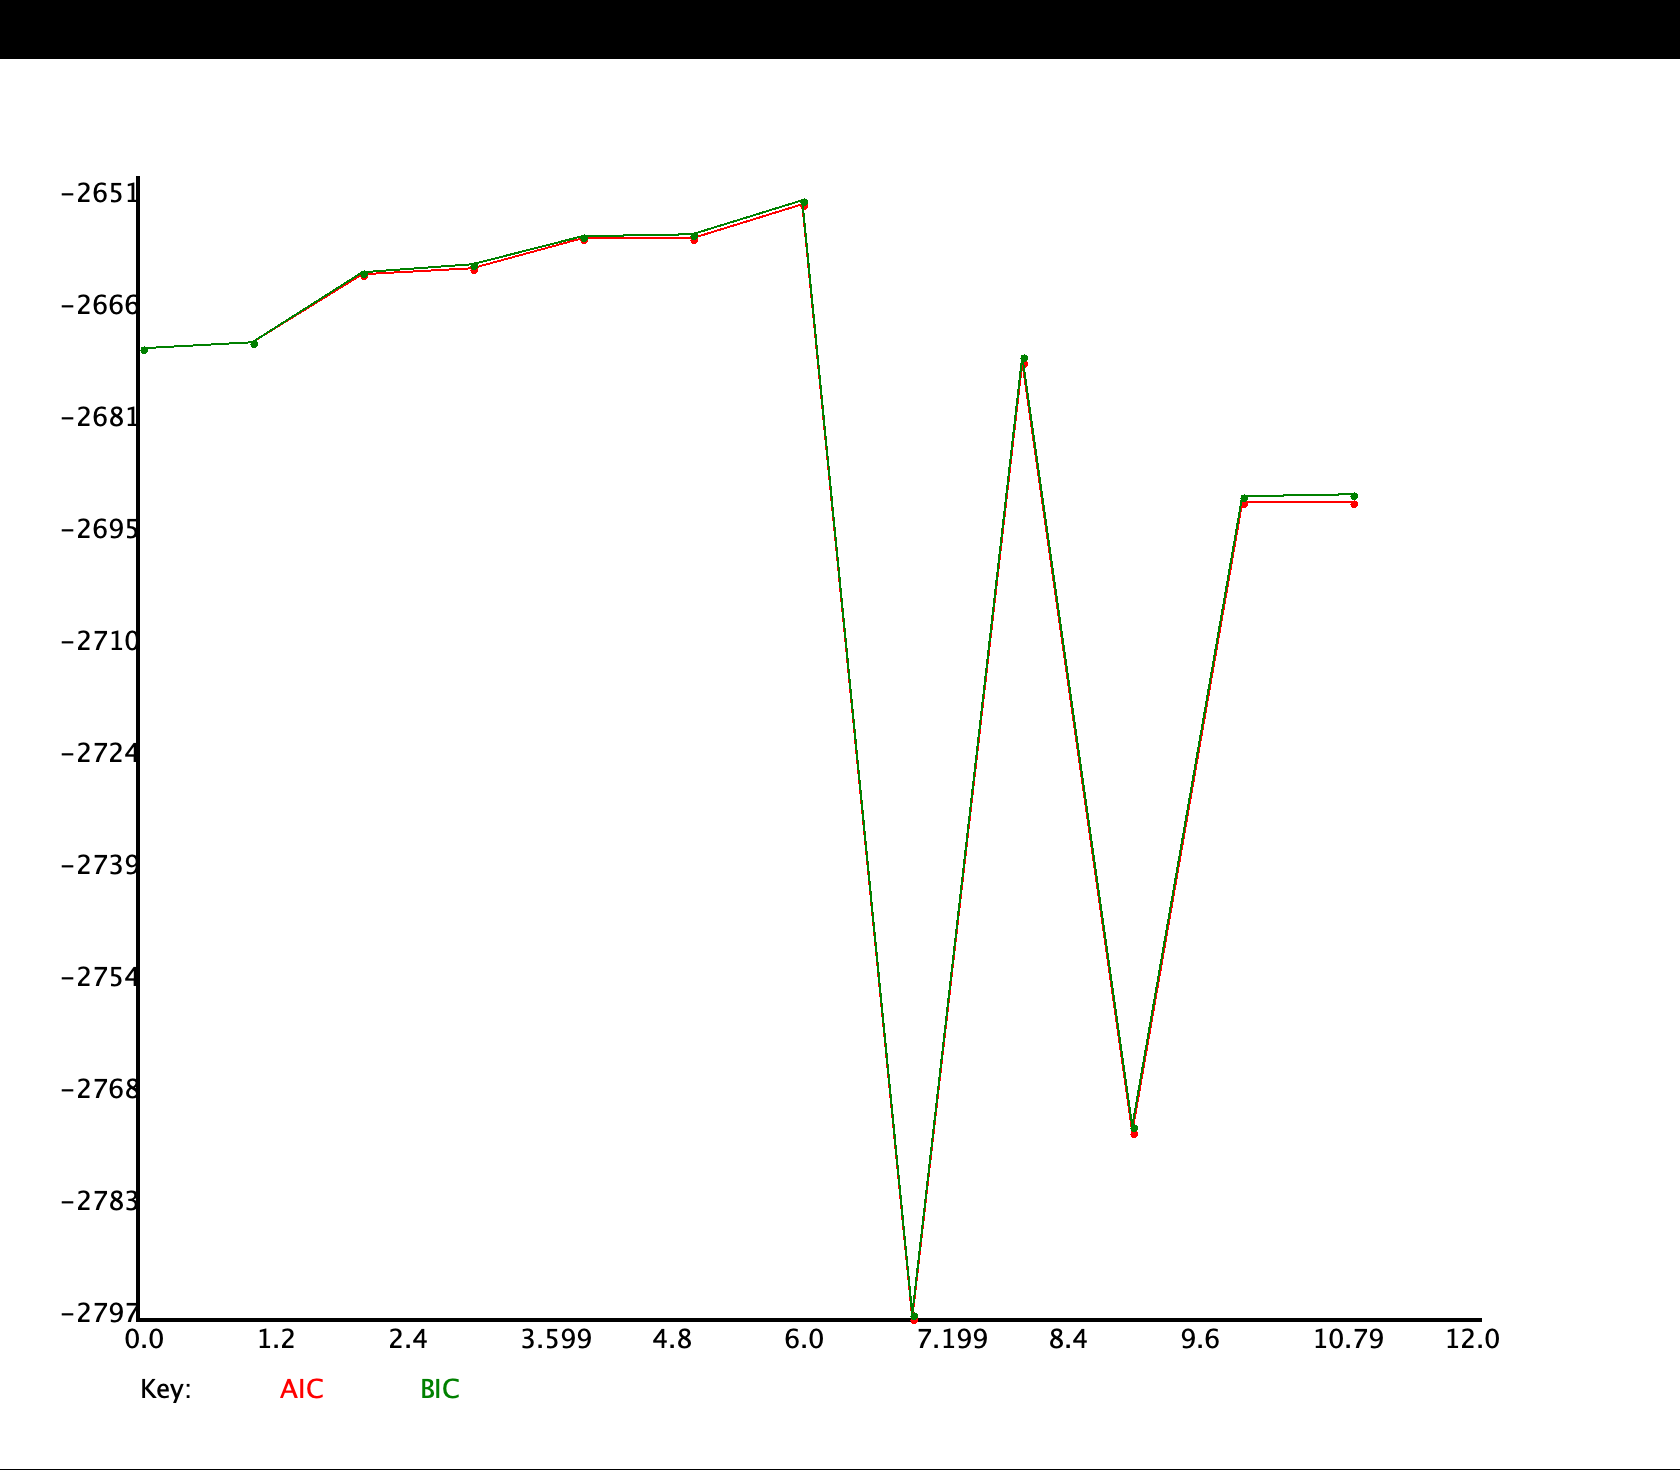
\includegraphics[width=\textwidth]{../House_Prices_Scalation_Plots/Scalation_Lasso_AIC_BIC_Forward.png}
     \end{subfigure}

     \vspace{10pt} % Add some vertical spacing between rows

     % Second Row
     \begin{subfigure}[b]{0.49\textwidth}
         \centering
         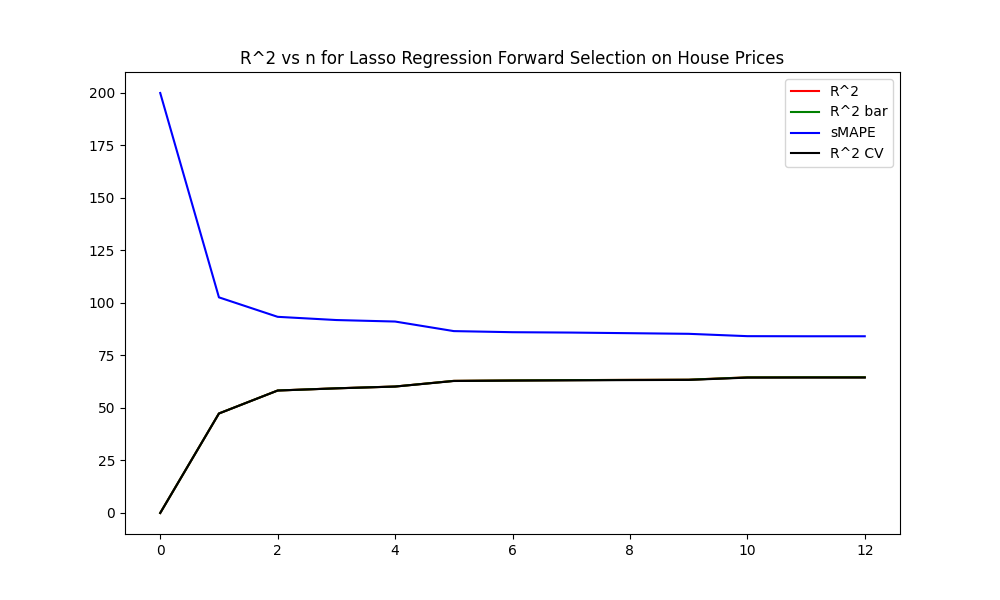
\includegraphics[width=\textwidth]{../House_Prices_Statsmodels_Plots/Statsmodels_Lasso_rSq_Forward.png}
     \end{subfigure}
     \hfill
     \begin{subfigure}[b]{0.49\textwidth}
         \centering
         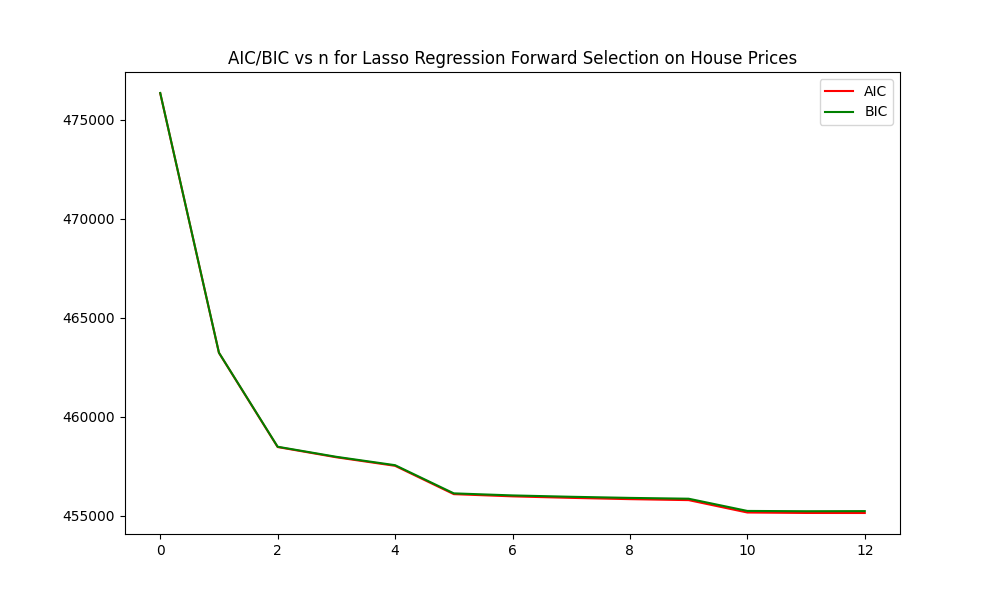
\includegraphics[width=\textwidth]{../House_Prices_Statsmodels_Plots/Statsmodels_Lasso_AIC_BIC_Forward.png}
     \end{subfigure}
     
     \caption{California House Prices Lasso Regression Forward Selection Quality of Fit Metrics\\ Top Left: Scalation $R^2$, Top Right: Scalation AIC/BIC\\ Bottom Left: Statsmodels $R^2$, Bottom Right: Statsmodels AIC/BIC}
     \label{fig:California House Prices Lasso Regression Forward Selection Quality of Fit Metrics}
\end{figure}

Scalation Backward Elimination Reversed: longitude, ocean proximity INLAND, median income, population, households, housing median age, ocean proximity ISLAND, latitude, ocean proximity NEAR OCEAN, ocean proximity NEAR BAY, total rooms, total bedrooms

Statsmodels Backward Elimination Reversed: Null, median income, latitude, longitude, total bedrooms, population, housing median age, ocean proximity INLAND, total rooms, households, ocean proximity ISLAND, ocean proximity NEAR OCEAN, ocean proximity NEAR BAY

\begin{figure}[H]
     \centering
     \captionsetup{justification=centering}
     % First Row
     \begin{subfigure}[b]{0.4\textwidth}
         \centering
         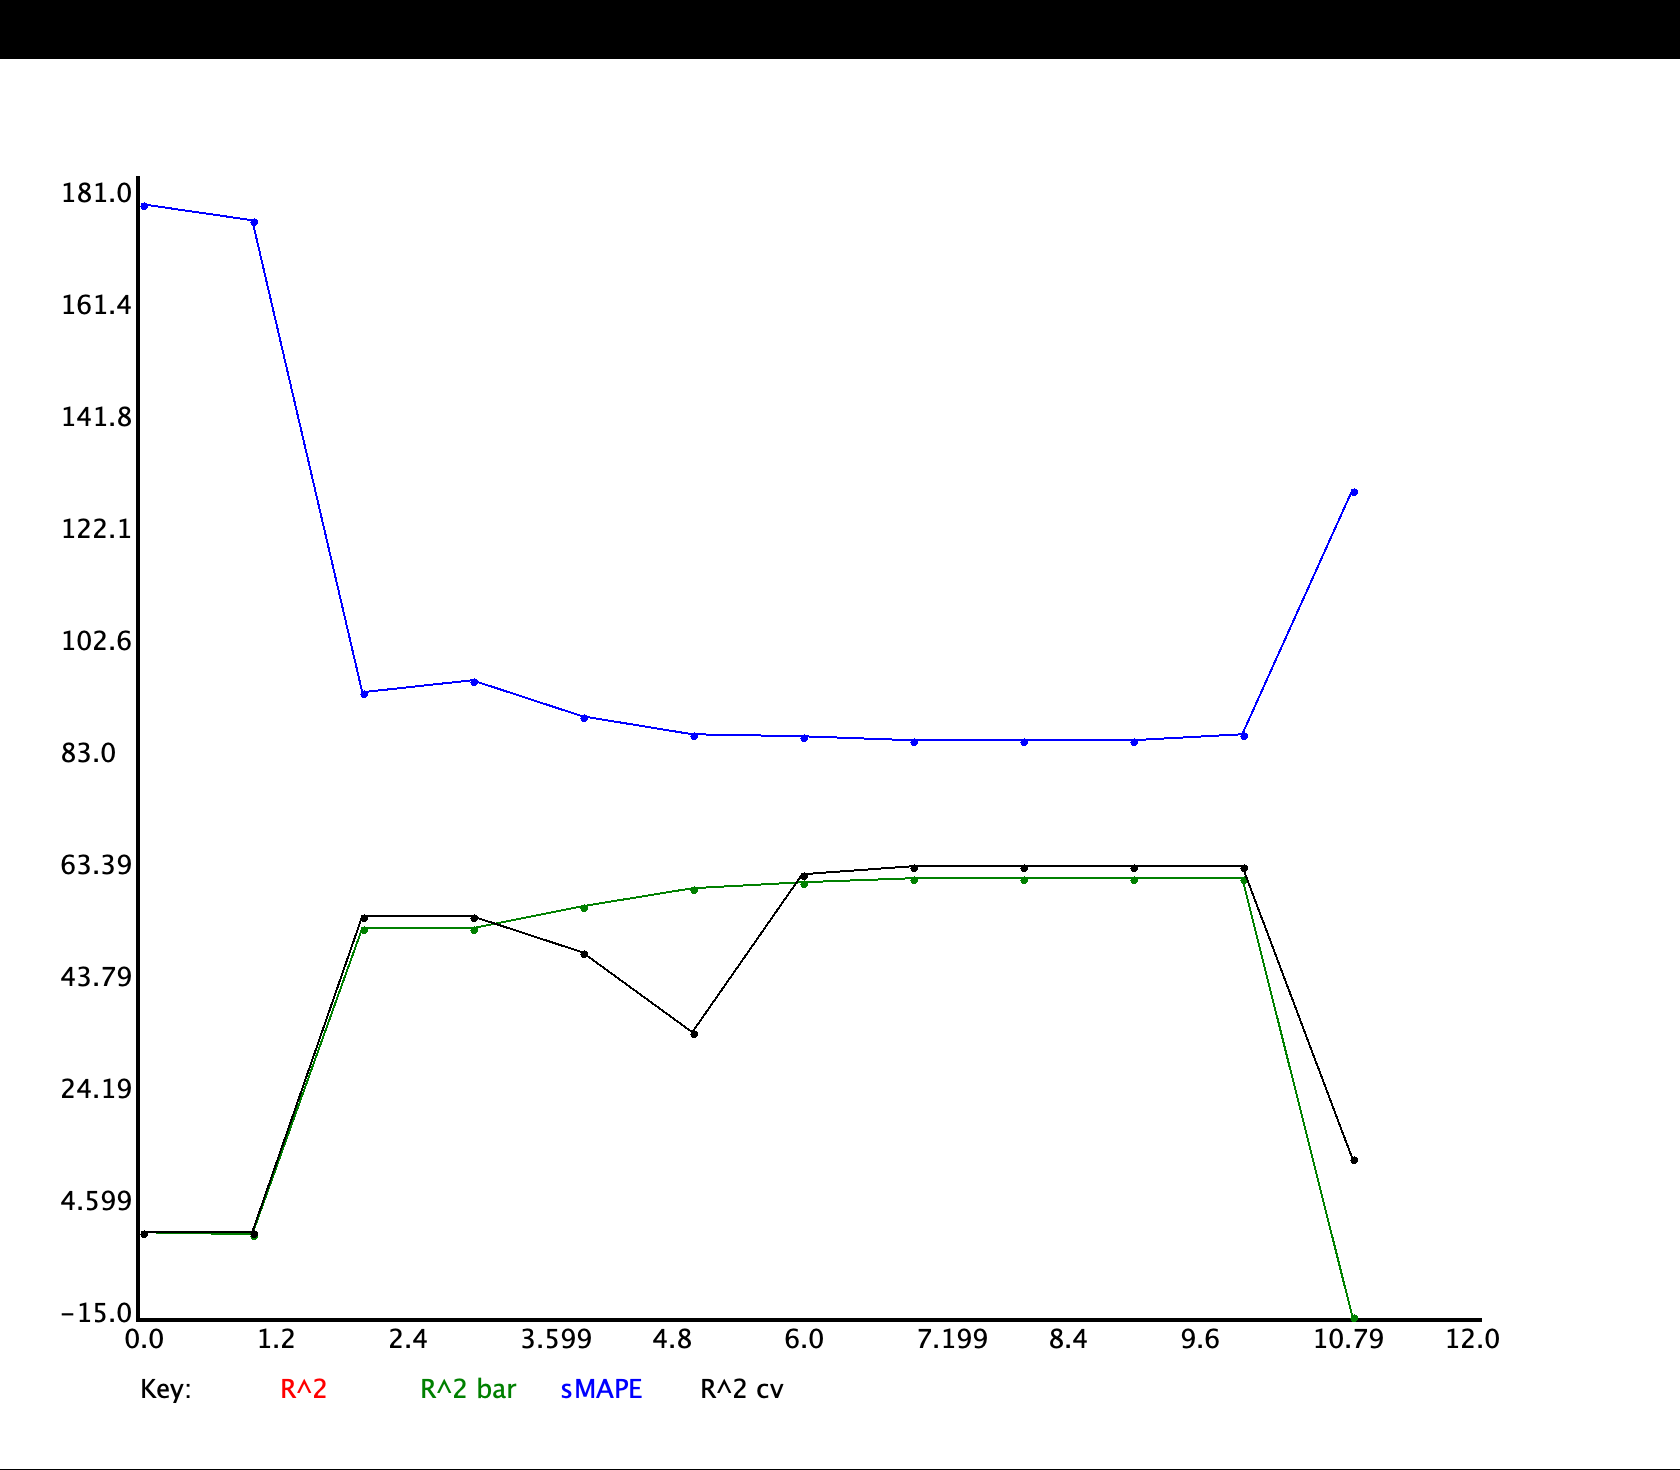
\includegraphics[width=\textwidth]{../House_Prices_Scalation_Plots/Scalation_Lasso_rSq_Backward.png}
     \end{subfigure}
     \hfill
     \begin{subfigure}[b]{0.4\textwidth}
         \centering
         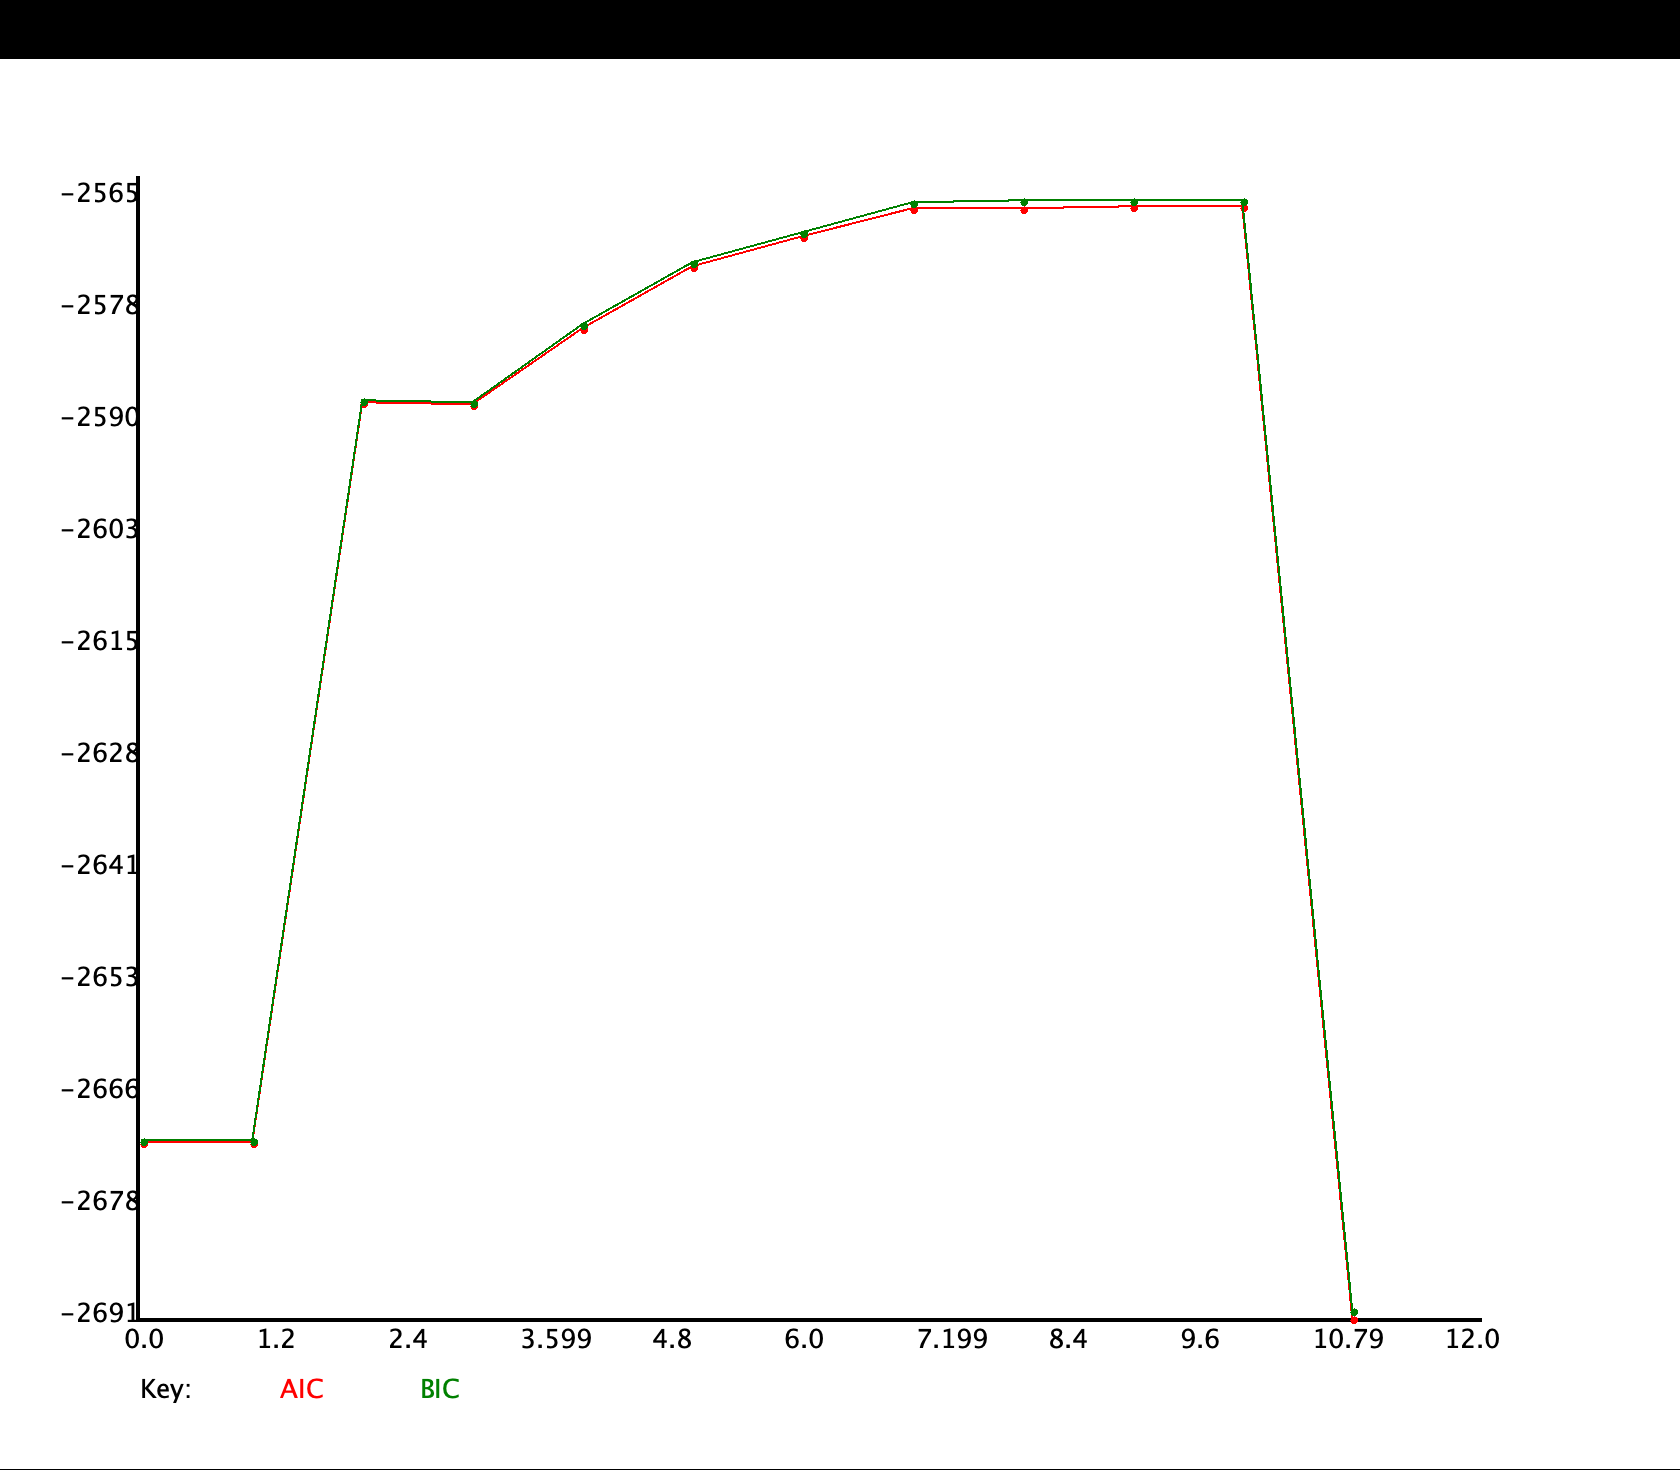
\includegraphics[width=\textwidth]{../House_Prices_Scalation_Plots/Scalation_Lasso_AIC_BIC_Backward.png}
     \end{subfigure}

     \vspace{10pt} % Add some vertical spacing between rows

     % Second Row
     \begin{subfigure}[b]{0.49\textwidth}
         \centering
         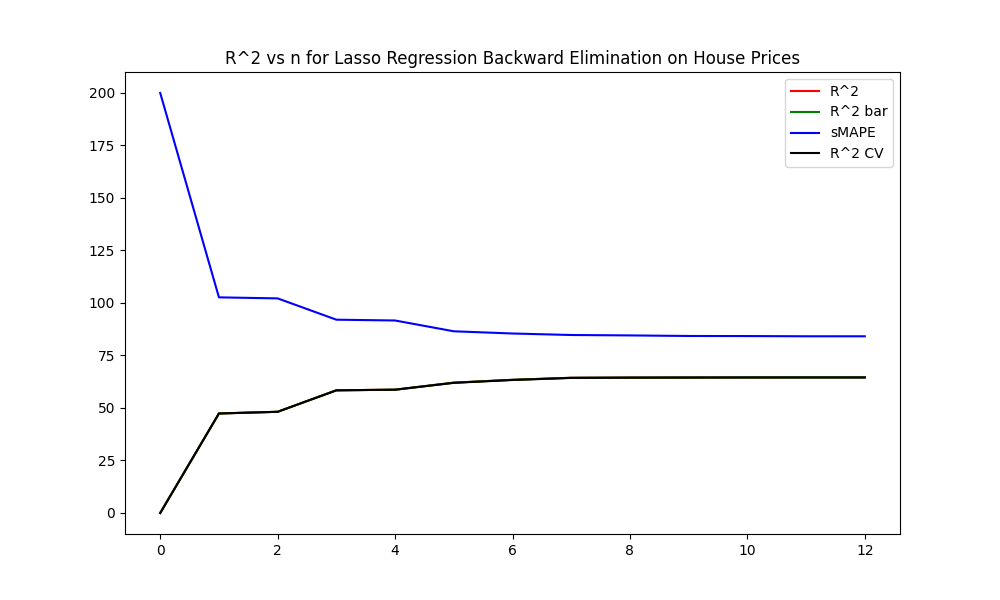
\includegraphics[width=\textwidth]{../House_Prices_Statsmodels_Plots/Statsmodels_Lasso_rSq_Backward.png}
     \end{subfigure}
     \hfill
     \begin{subfigure}[b]{0.49\textwidth}
         \centering
         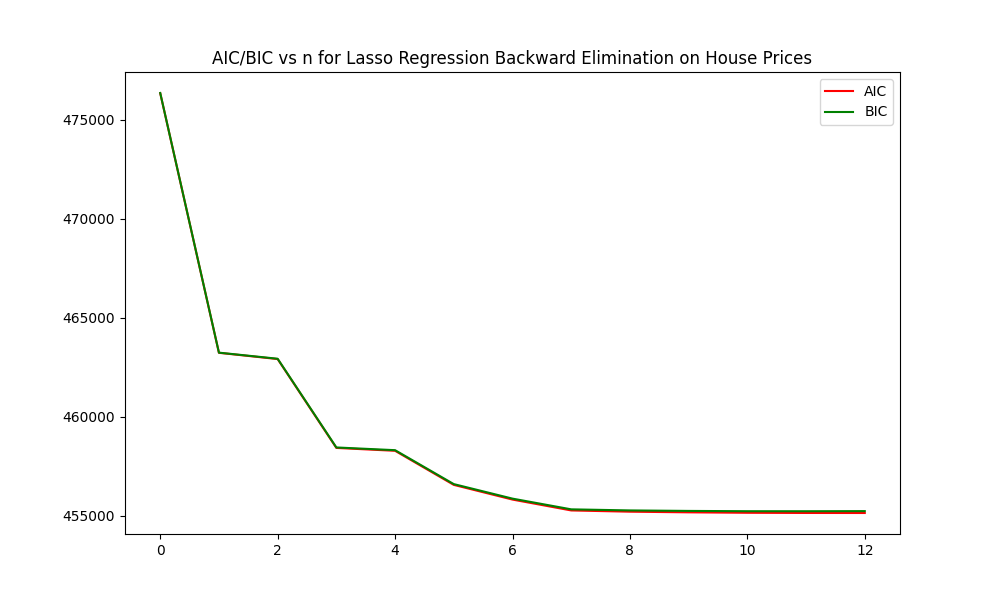
\includegraphics[width=\textwidth]{../House_Prices_Statsmodels_Plots/Statsmodels_Lasso_AIC_BIC_Backward.png}
     \end{subfigure}
     
     \caption{California House Prices Lasso Regression Reversed Backward Elimination Quality of Fit Metrics\\ Top Left: Scalation $R^2$, Top Right: Scalation AIC/BIC\\ Bottom Left: Statsmodels $R^2$, Bottom Right: Statsmodels AIC/BIC}
     \label{fig:California House Prices Lasso Regression Reversed Backward Elimination Quality of Fit Metrics}
\end{figure}

Scalation Stepwise Selection: longitude, total rooms, population, households, latitude, housing median age, ocean proximity INLAND, ocean proximity NEAR BAY, ocean proximity ISLAND

Statsmodels Stepwise Selection: Null, median income, ocean proximity INLAND, housing median age, total bedrooms, population, households, total rooms, ocean proximity NEAR OCEAN, longitude, latitude, ocean proximity ISLAND, ocean proximity NEAR BAY

\begin{figure}[H]
     \centering
     \captionsetup{justification=centering}
     % First Row
     \begin{subfigure}[b]{0.4\textwidth}
         \centering
         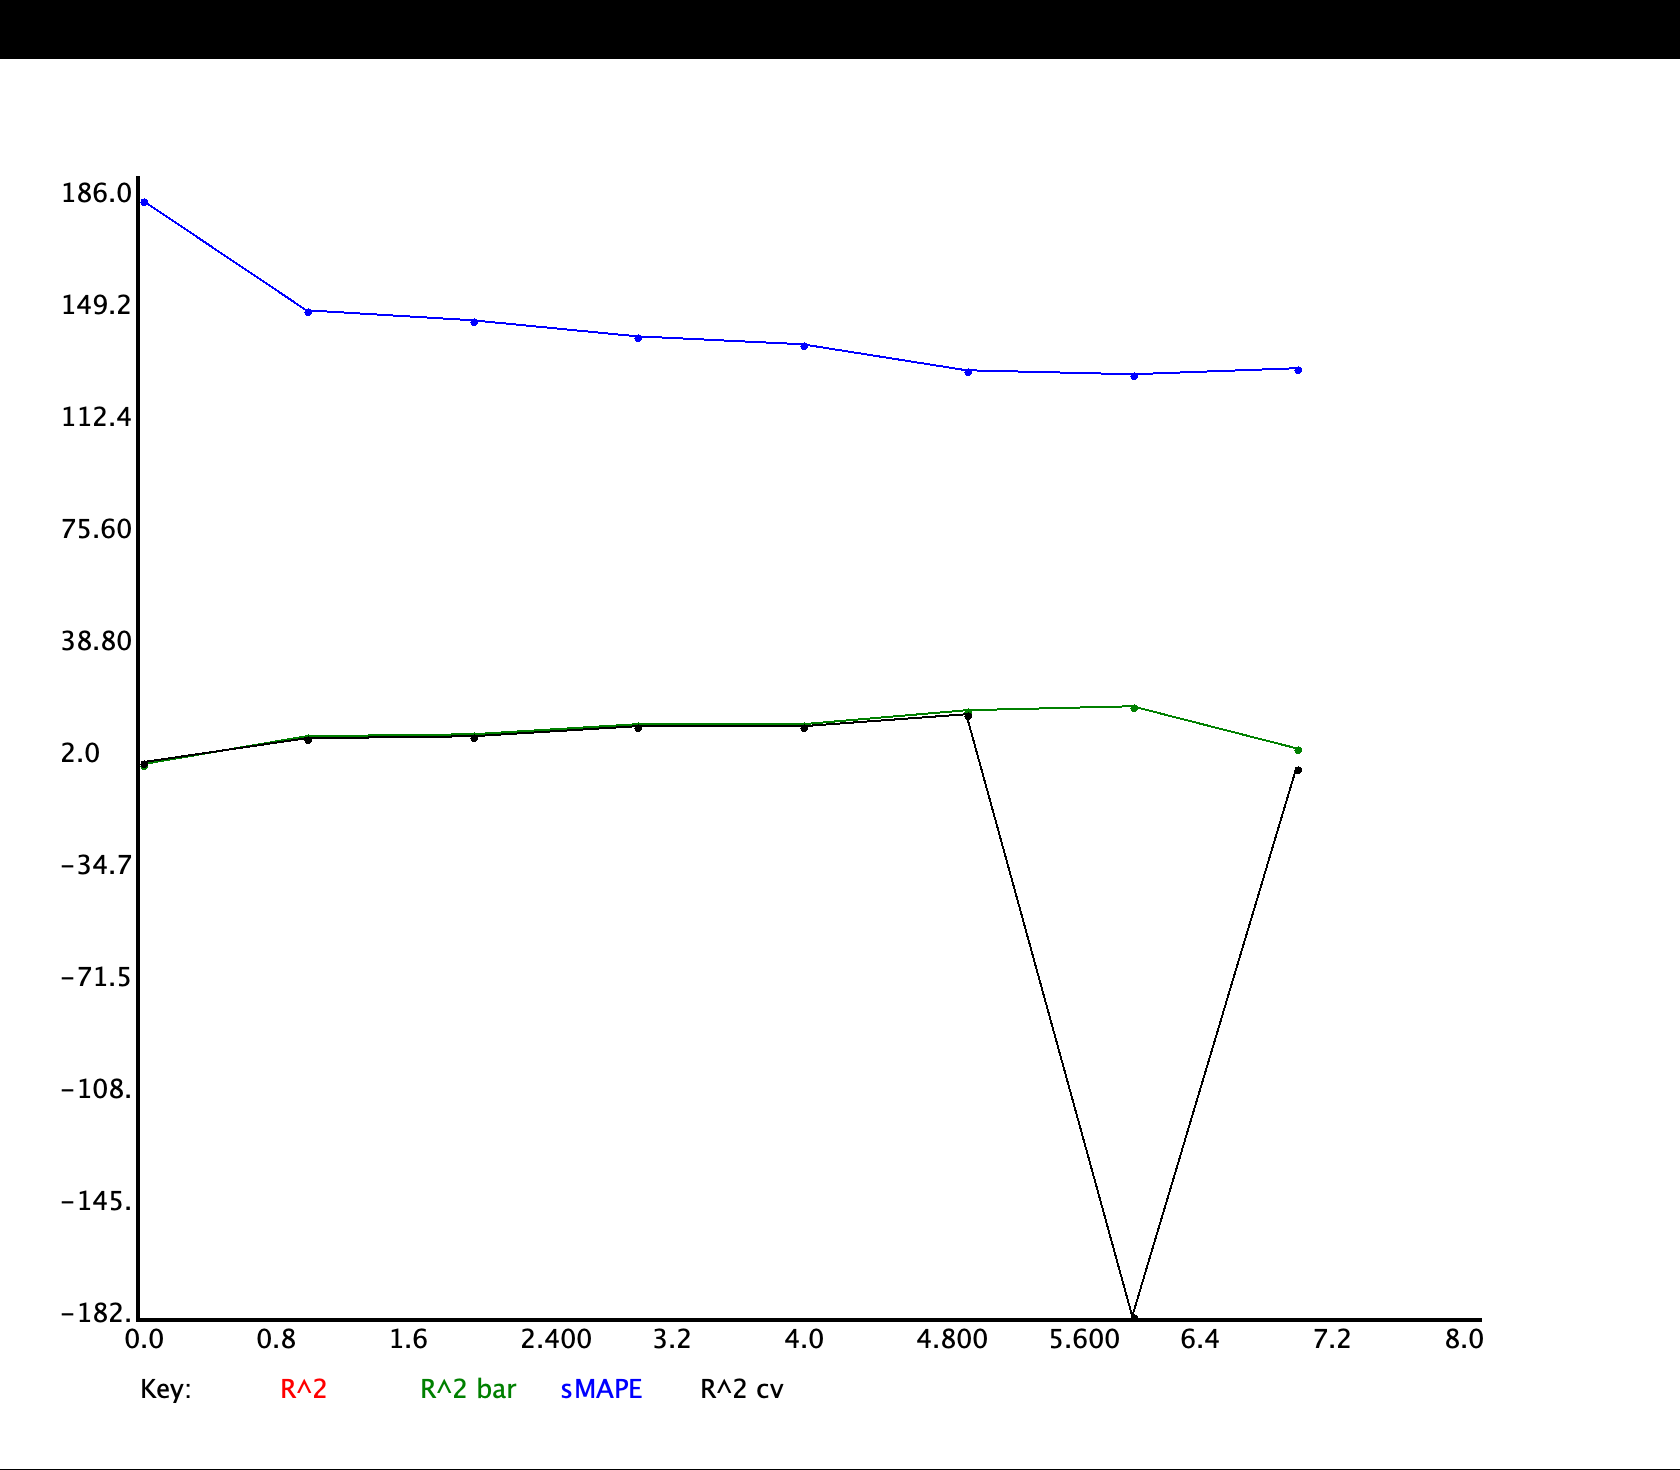
\includegraphics[width=\textwidth]{../House_Prices_Scalation_Plots/Scalation_Lasso_rSq_Stepwise.png}
     \end{subfigure}
     \hfill
     \begin{subfigure}[b]{0.4\textwidth}
         \centering
         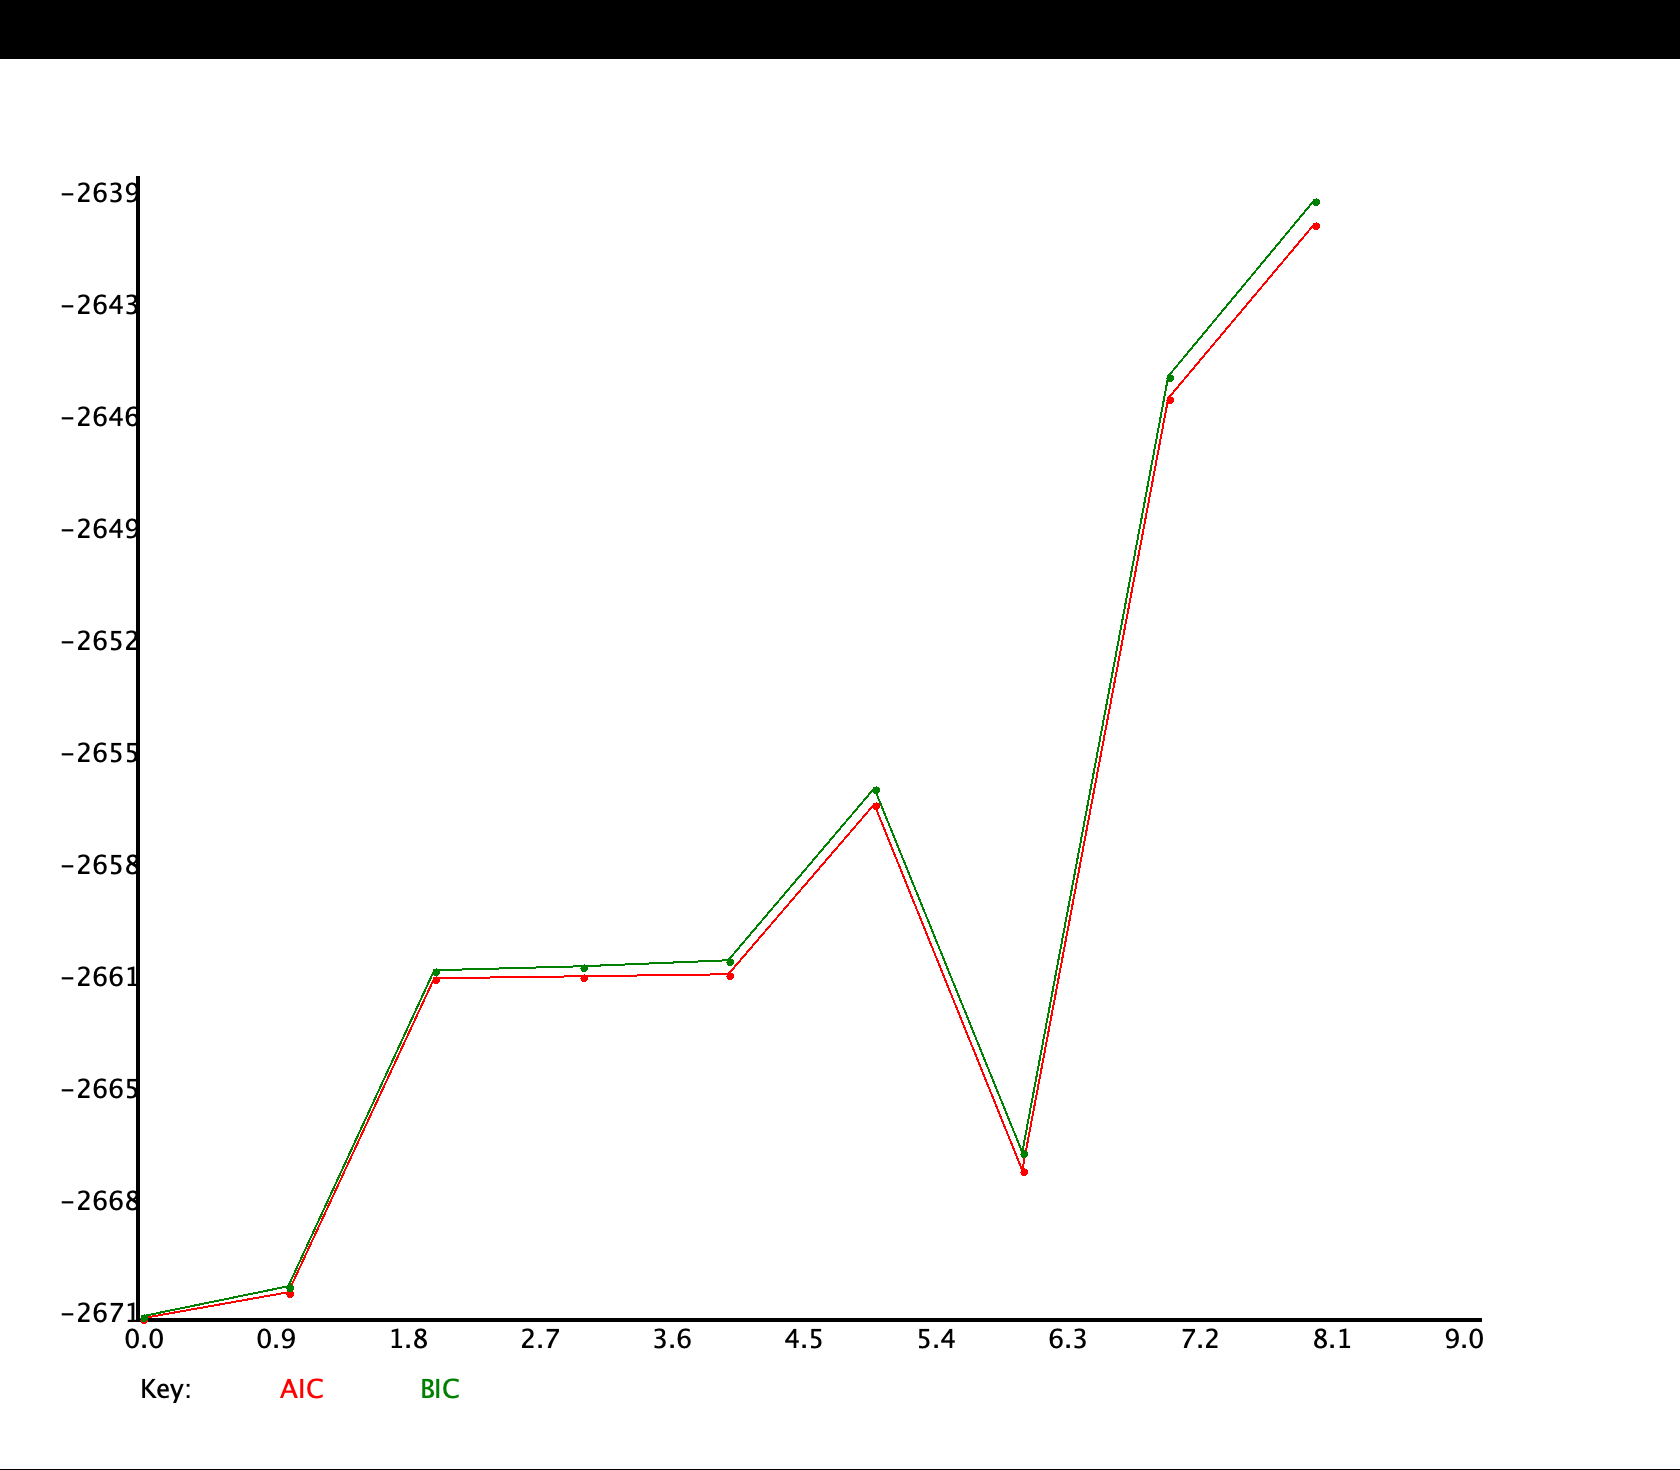
\includegraphics[width=\textwidth]{../House_Prices_Scalation_Plots/Scalation_Lasso_AIC_BIC_Stepwise.png}
     \end{subfigure}

     \vspace{10pt} % Add some vertical spacing between rows

     % Second Row
     \begin{subfigure}[b]{0.49\textwidth}
         \centering
         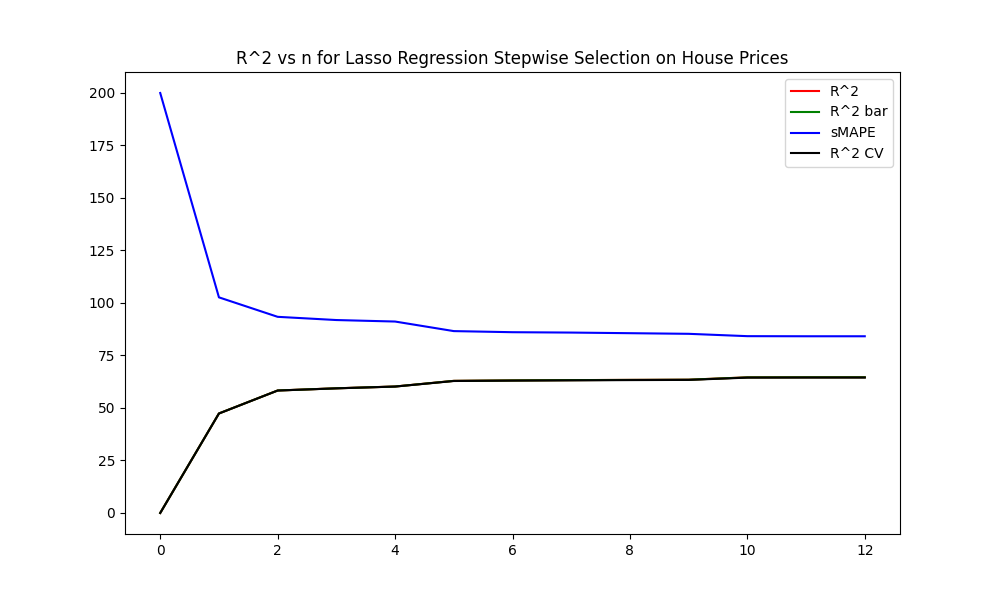
\includegraphics[width=\textwidth]{../House_Prices_Statsmodels_Plots/Statsmodels_Lasso_rSq_Stepwise.png}
     \end{subfigure}
     \hfill
     \begin{subfigure}[b]{0.49\textwidth}
         \centering
         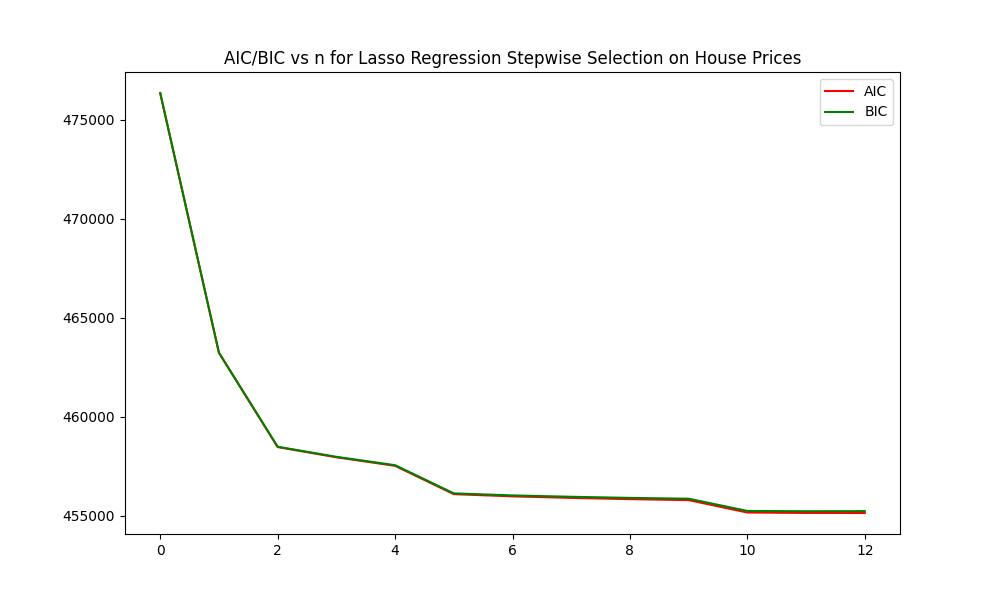
\includegraphics[width=\textwidth]{../House_Prices_Statsmodels_Plots/Statsmodels_Lasso_AIC_BIC_Stepwise.png}
     \end{subfigure}
     
     \caption{California House Prices Lasso Regression Stepwise Selection Quality of Fit Metrics\\ Top Left: Scalation $R^2$, Top Right: Scalation AIC/BIC\\ Bottom Left: Statsmodels $R^2$, Bottom Right: Statsmodels AIC/BIC}
     \label{fig:California House Prices Lasso Regression Stepwise Selection Quality of Fit Metrics}
\end{figure}

\subsection{Sqrt Transformation}

\subsubsection{Quality of Fit}

\begin{table}[H]
\centering
\caption{Scalation - California House Prices Sqrt Transformation}
\label{tab:Scalation - House Prices Sqrt Transformation}
\begin{tabular}{|c|c|c|} \hline 
Metric & In-Sample & 80-20 Split \\ \hline \hline 
rSq &0.632150 & 0.622490 \\ \hline 
rSqBar &0.631934 &      0.622268 \\ \hline 
sst &2.72264e+14 &      5.31945e+13 \\ \hline 
sse &1.00152e+14 &      2.00815e+13 \\ \hline 
sde &69835.0 &  70059.9 \\ \hline 
mse0 &4.90151e+09 &     4.91470e+09 \\ \hline 
rmse &70010.8 & 70104.9 \\ \hline 
mae &48220.5 &  47894.5 \\ \hline 
smape &24.2465 &        24.3387 \\ \hline 
m &20433.0 &    4086.00 \\ \hline 
dfr &12.0000 &  12.0000 \\ \hline 
df &20420.0 &   20420.0 \\ \hline 
fStat &2924.31 &        2805.94 \\ \hline 
aic &-256926 &  -51362.3 \\ \hline 
bic &-256823 &  -51280.2 \\ \hline 
\end{tabular}
\end{table}

\begin{table}[H]
\centering
\caption{Statsmodels - California House Prices Sqrt Transformation}
\label{tab:Statsmodels - House Prices Sqrt Transformation}
\begin{tabular}{|c|c|c|}\hline
Metric & In-Sample & 80-20 Split \\ \hline \hline
rSq & 0.6689 & 0.6384 \\ \hline
rSqBar & 0.6687 & 0.6373 \\ \hline
sst & 307417239.0954 & 54723646809444.8438 \\ \hline
sse & 101790254.8606 & 19789737392465.0977 \\ \hline
sde & 70.6033 & 69696.2647 \\ \hline
mse0 & 4984.8313 & 4842118275.6215 \\ \hline
rmse & 70.6033 & 69585.3309 \\ \hline
mae & 48220.5150 & 48238.7593 \\ \hline
smape & 24.2465 & 24.1385 \\ \hline
m & 20433.0000 & 4087.0000 \\ \hline
dfr & 12.0000 & 13.0000 \\ \hline
df & 20420.0000 & 4074.0000 \\ \hline
fStat & 3437.5450 & 553.2034 \\ \hline
aic & 231969.0638 & 91168.6263 \\ \hline
bic & 232072.0875 & 91250.7286 \\ \hline
\end{tabular}
\end{table}

\begin{table}[H]
\centering
\caption{Scalation - California House Prices Sqrt Transformation CV}
\label{tab:Scalation - House Prices Sqrt Transformation CV}
\begin{tabular}{|c|c|c|c|c|c|}\hline
Metric & num folds & min & max & mean & stdev \\ \hline \hline
rSq & 5 & 0.593 & 0.649 & 0.631 & 0.024 \\ \hline
rSqBar & 5 & 0.593 & 0.649 & 0.631 & 0.024 \\ \hline
sst & 5 & 53194492241132.980 & 57310203956796.625 & 54411355017051.000 & 1675890609056.710 \\ \hline
sse & 5 & 18995823093517.258 & 23315033455283.805 & 20099127442911.520 & 1854345601204.321 \\ \hline
sde & 5 & 68035.044 & 75168.723 & 69898.401 & 3067.760 \\ \hline
mse0 & 5 & 4649002225.530 & 5706077693.413 & 4919022869.043 & 453829075.185 \\ \hline
rmse & 5 & 68183.592 & 75538.584 & 70078.908 & 3156.245 \\ \hline
mae & 5 & 46979.443 & 51209.842 & 48279.153 & 1693.616 \\ \hline
smape & 5 & 23.649 & 24.699 & 24.272 & 0.406 \\ \hline
m & 5 & 4086.000 & 4086.000 & 4086.000 & 0.000 \\ \hline
dfr & 5 & 12.000 & 12.000 & 12.000 & 0.000 \\ \hline
df & 5 & 20420.000 & 20420.000 & 20420.000 & 0.000 \\ \hline
fStat & 5 & 2481.165 & 3145.436 & 2925.139 & 282.419 \\ \hline
aic & 5 & -51691.817 & -51251.727 & -51364.144 & 188.942 \\ \hline
bic & 5 & -51609.718 & -51169.628 & -51282.045 & 188.942 \\ \hline
\end{tabular}
\end{table}

\begin{table}[H]
\centering
\caption{Statsmodels - California House Prices Sqrt Transformation CV}
\label{tab:Statsmodels - House Prices Sqrt Transformation CV}
\begin{tabular}{|c|c|c|c|c|c|}\hline
Metric & num folds & min & max & mean & stdev \\ \hline \hline
rSq & 5 & 0.6191 & 0.6458 & 0.6313 & 0.0098 \\ \hline
rSqBar & 5 & 0.6180 & 0.6447 & 0.6302 & 0.0098 \\ \hline
sst & 5 & 53541750406767.3438 & 54912923487891.5781 & 54447676367709.7031 & 499826929365.4288 \\ \hline
sse & 5 & 19452132950120.8516 & 20463182416338.9062 & 20070256659186.4102 & 388141207054.1924 \\ \hline
sde & 5 & 69099.2132 & 70880.9260 & 70188.6762 & 683.7286 \\ \hline
mse0 & 5 & 4759513812.1167 & 5008121002.5303 & 4911244568.8971 & 95422756.2347 \\ \hline
rmse & 5 & 68989.2297 & 70768.0790 & 70076.9476 & 682.6301 \\ \hline
mae & 5 & 47287.9994 & 48864.9909 & 48266.6663 & 530.5118 \\ \hline
smape & 5 & 23.8757 & 24.6190 & 24.2655 & 0.2478 \\ \hline
m & 5 & 4086.0000 & 4087.0000 & 4086.6000 & 0.4899 \\ \hline
dfr & 5 & 13.0000 & 13.0000 & 13.0000 & 0.0000 \\ \hline
df & 5 & 4073.0000 & 4074.0000 & 4073.6000 & 0.4899 \\ \hline
fStat & 5 & 509.2140 & 571.2929 & 537.1572 & 22.7437 \\ \hline
aic & 5 & 91098.3022 & 91284.0586 & 91216.8498 & 71.9445 \\ \hline
bic & 5 & 91180.4046 & 91366.1578 & 91298.9509 & 71.9435 \\ \hline
\end{tabular}
\end{table}

\begin{figure}[H]
     \centering
     \captionsetup{justification=centering}
     % First Row
     \begin{subfigure}[b]{0.4\textwidth}
         \centering
         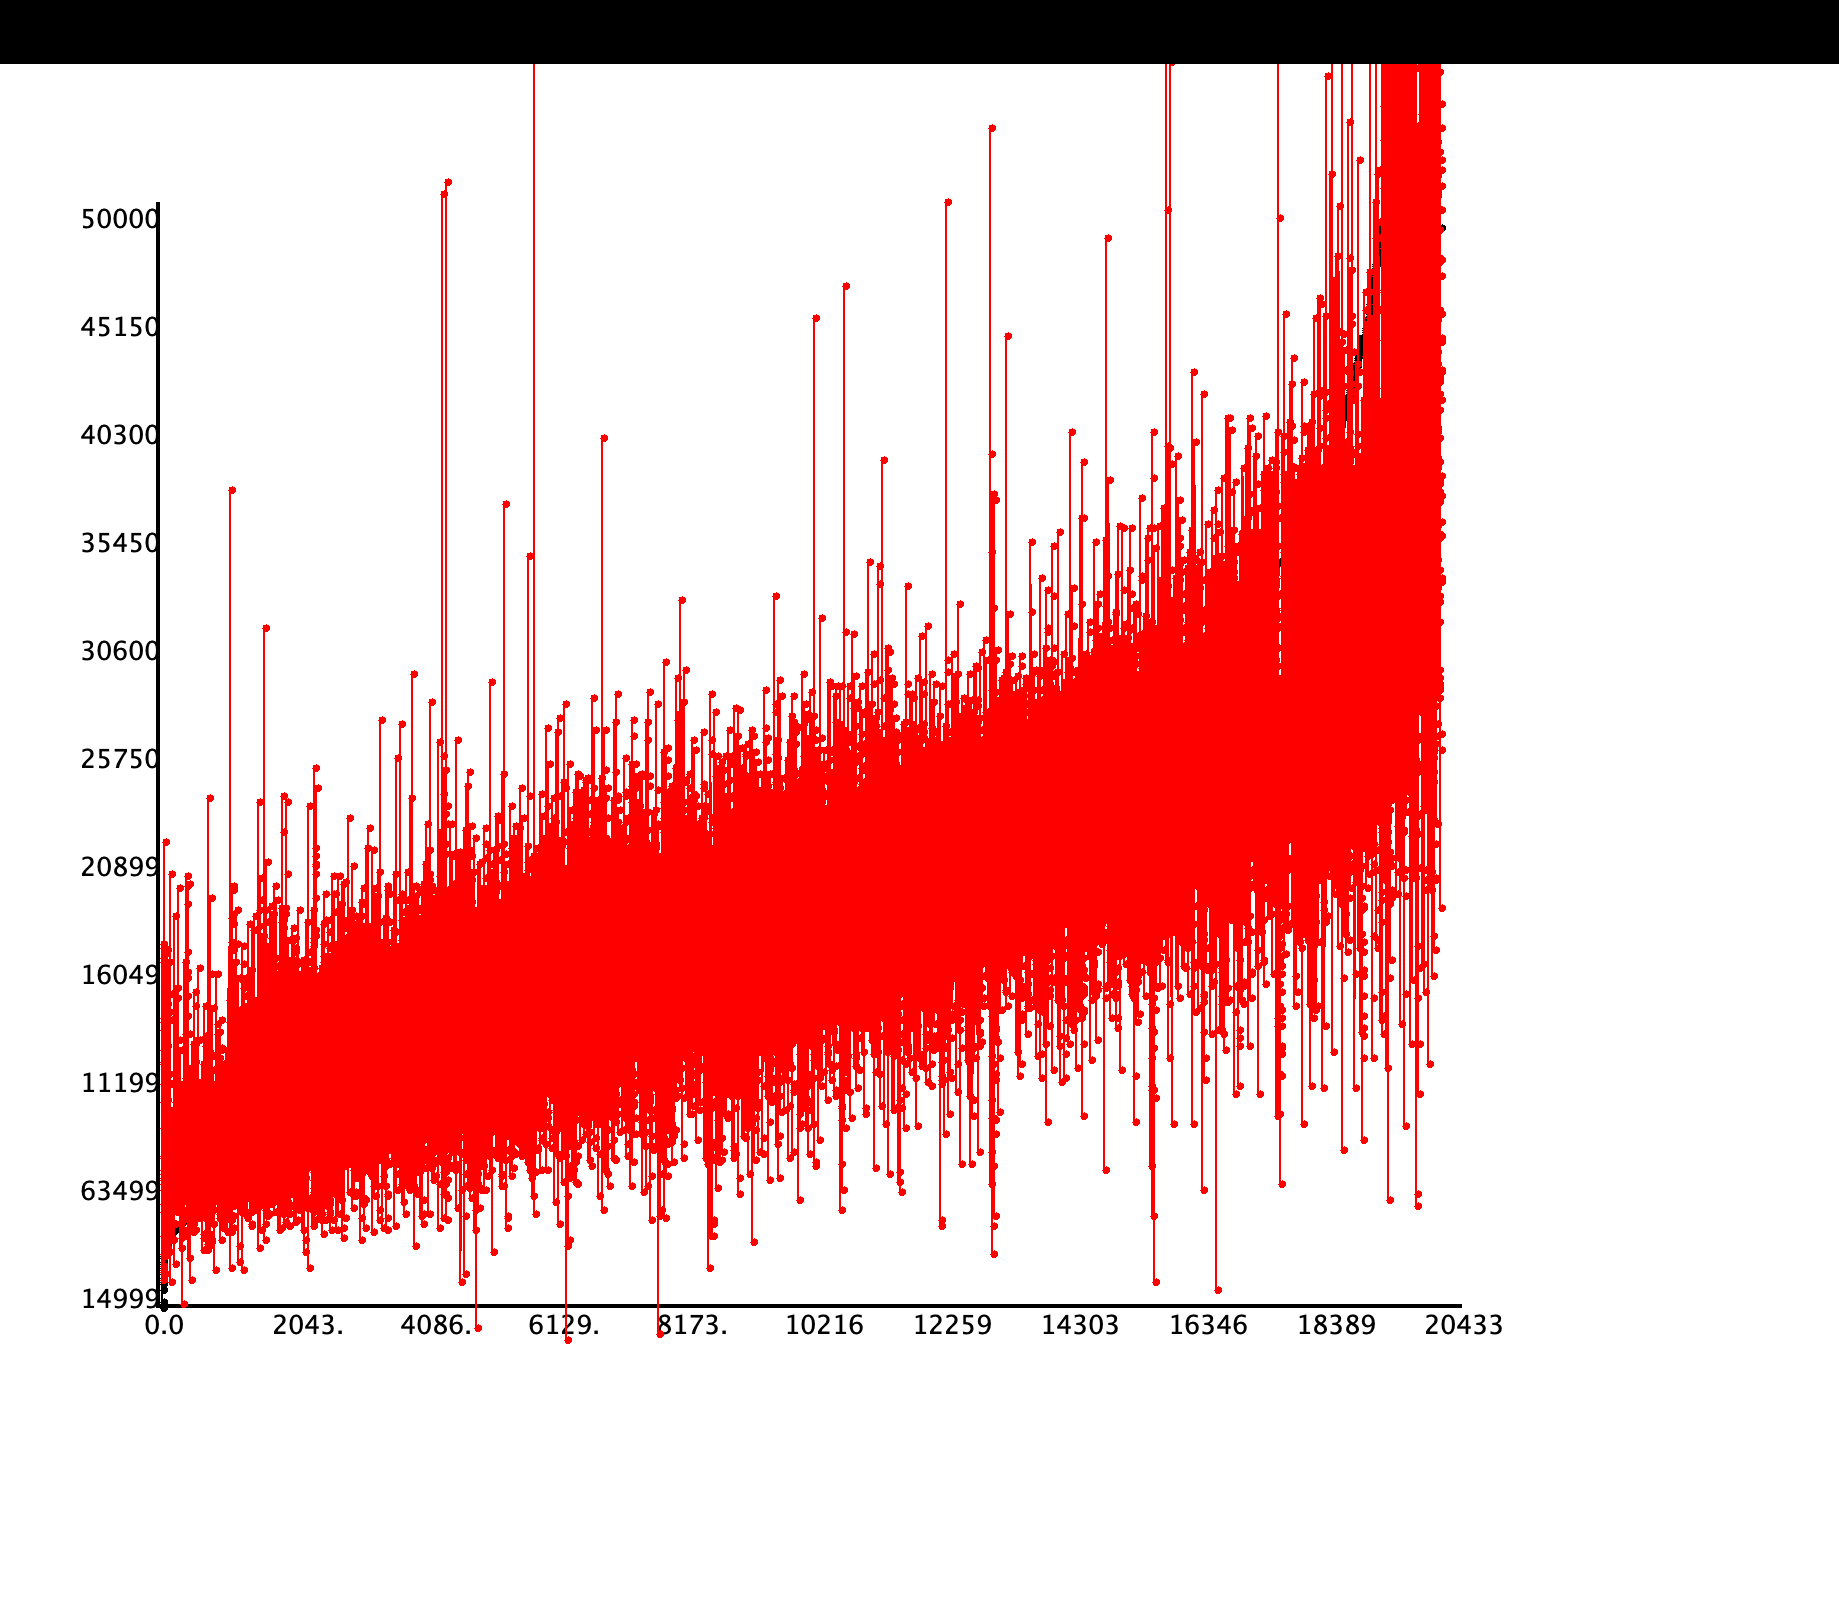
\includegraphics[width=\textwidth]{../House_Prices_Scalation_Plots/Scalation_Sqrt_In_Sample.png}
     \end{subfigure}
     \hfill
     \begin{subfigure}[b]{0.4\textwidth}
         \centering
         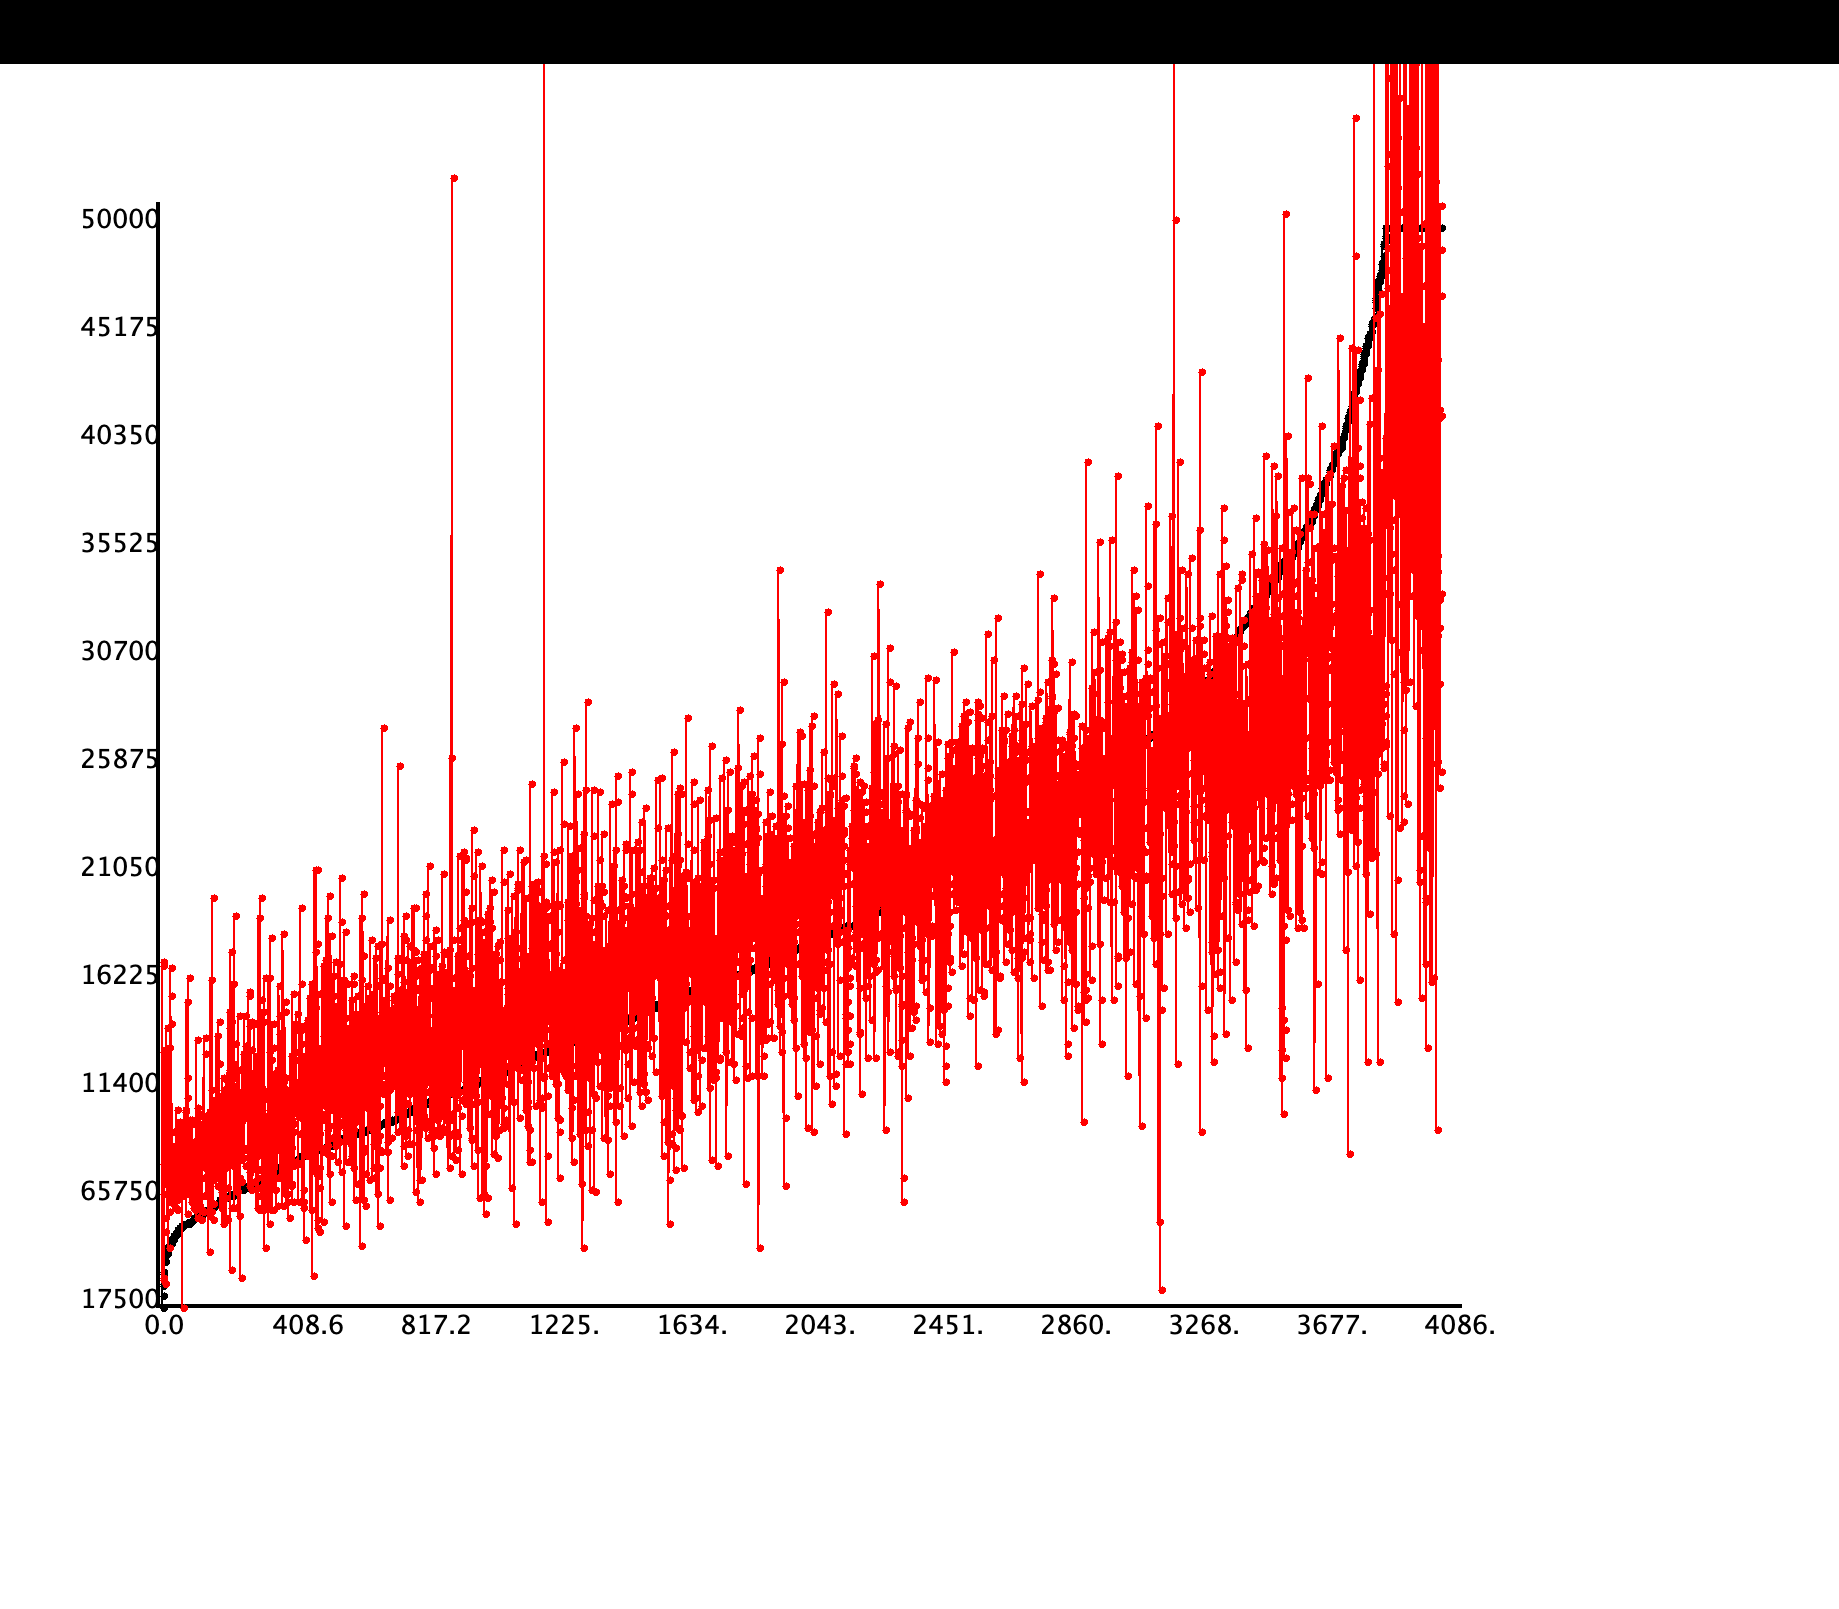
\includegraphics[width=\textwidth]{../House_Prices_Scalation_Plots/Scalation_Sqrt_80_20.png}
     \end{subfigure}

     \vspace{10pt} % Add some vertical spacing between rows

     % Second Row
     \begin{subfigure}[b]{0.49\textwidth}
         \centering
         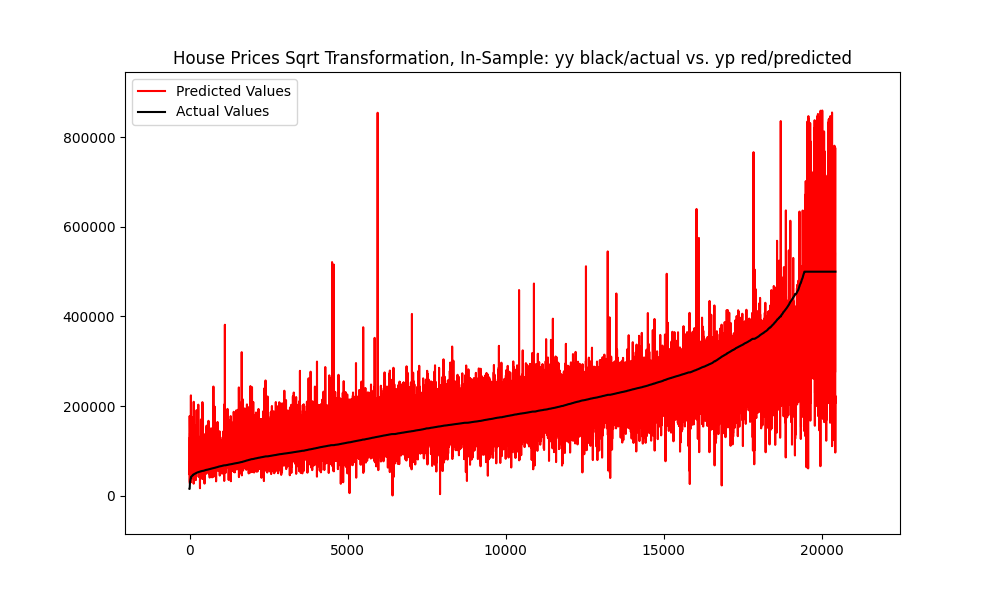
\includegraphics[width=\textwidth]{../House_Prices_Statsmodels_Plots/Statsmodels_Sqrt_In_Sample.png}
     \end{subfigure}
     \hfill
     \begin{subfigure}[b]{0.49\textwidth}
         \centering
         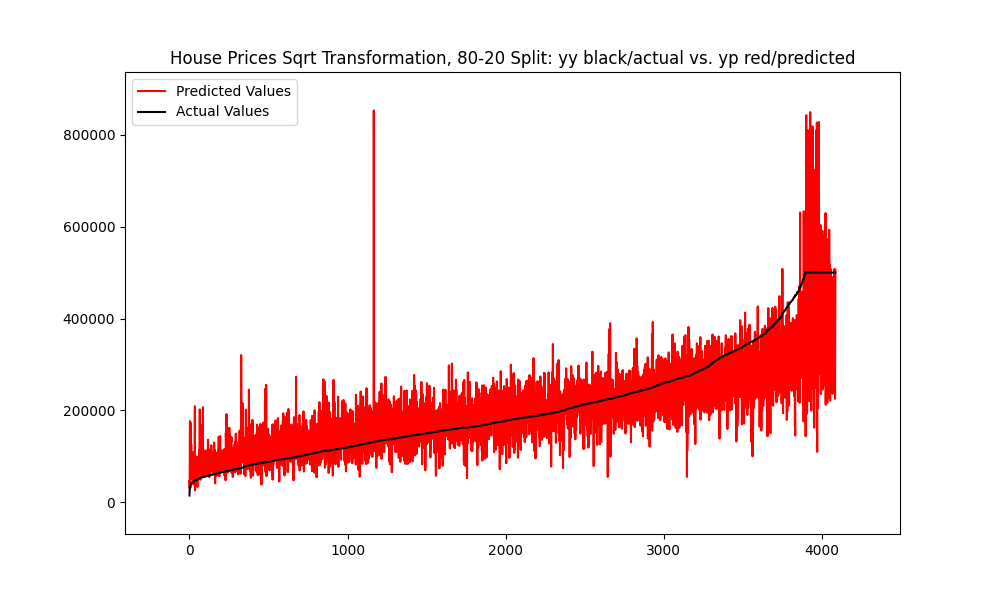
\includegraphics[width=\textwidth]{../House_Prices_Statsmodels_Plots/Statsmodels_Sqrt_80_20.png}
     \end{subfigure}
     
     \caption{California House Prices Sqrt Transformation Plots\\ Top Left: Scalation In-Sample, Top Right: Scalation Out-of-Sample\\ Bottom Left: Statsmodels In-Sample, Bottom Right: Statsmodels Out-of-Sample\\ black: actual y-values, red: predicted y-values}
     \label{fig:California House Prices Sqrt Transformation Plots}
\end{figure}

\subsubsection{Feature Selection}

Scalation Forward Selection: intercept, population, longitude, ocean proximity ISLAND, ocean proximity NEAR OCEAN, housing median age, total bedrooms, households, ocean proximity NEAR BAY, total rooms, latitude, ocean proximity INLAND, median income

Statsmodels Forward Selection: intercept, median income, ocean proximity INLAND, housing median age, total bedrooms, population, households, ocean proximity NEAR OCEAN, longitude, latitude, ocean proximity ISLAND, ocean proximity NEAR BAY, total rooms

\begin{figure}[H]
     \centering
     \captionsetup{justification=centering}
     % First Row
     \begin{subfigure}[b]{0.4\textwidth}
         \centering
         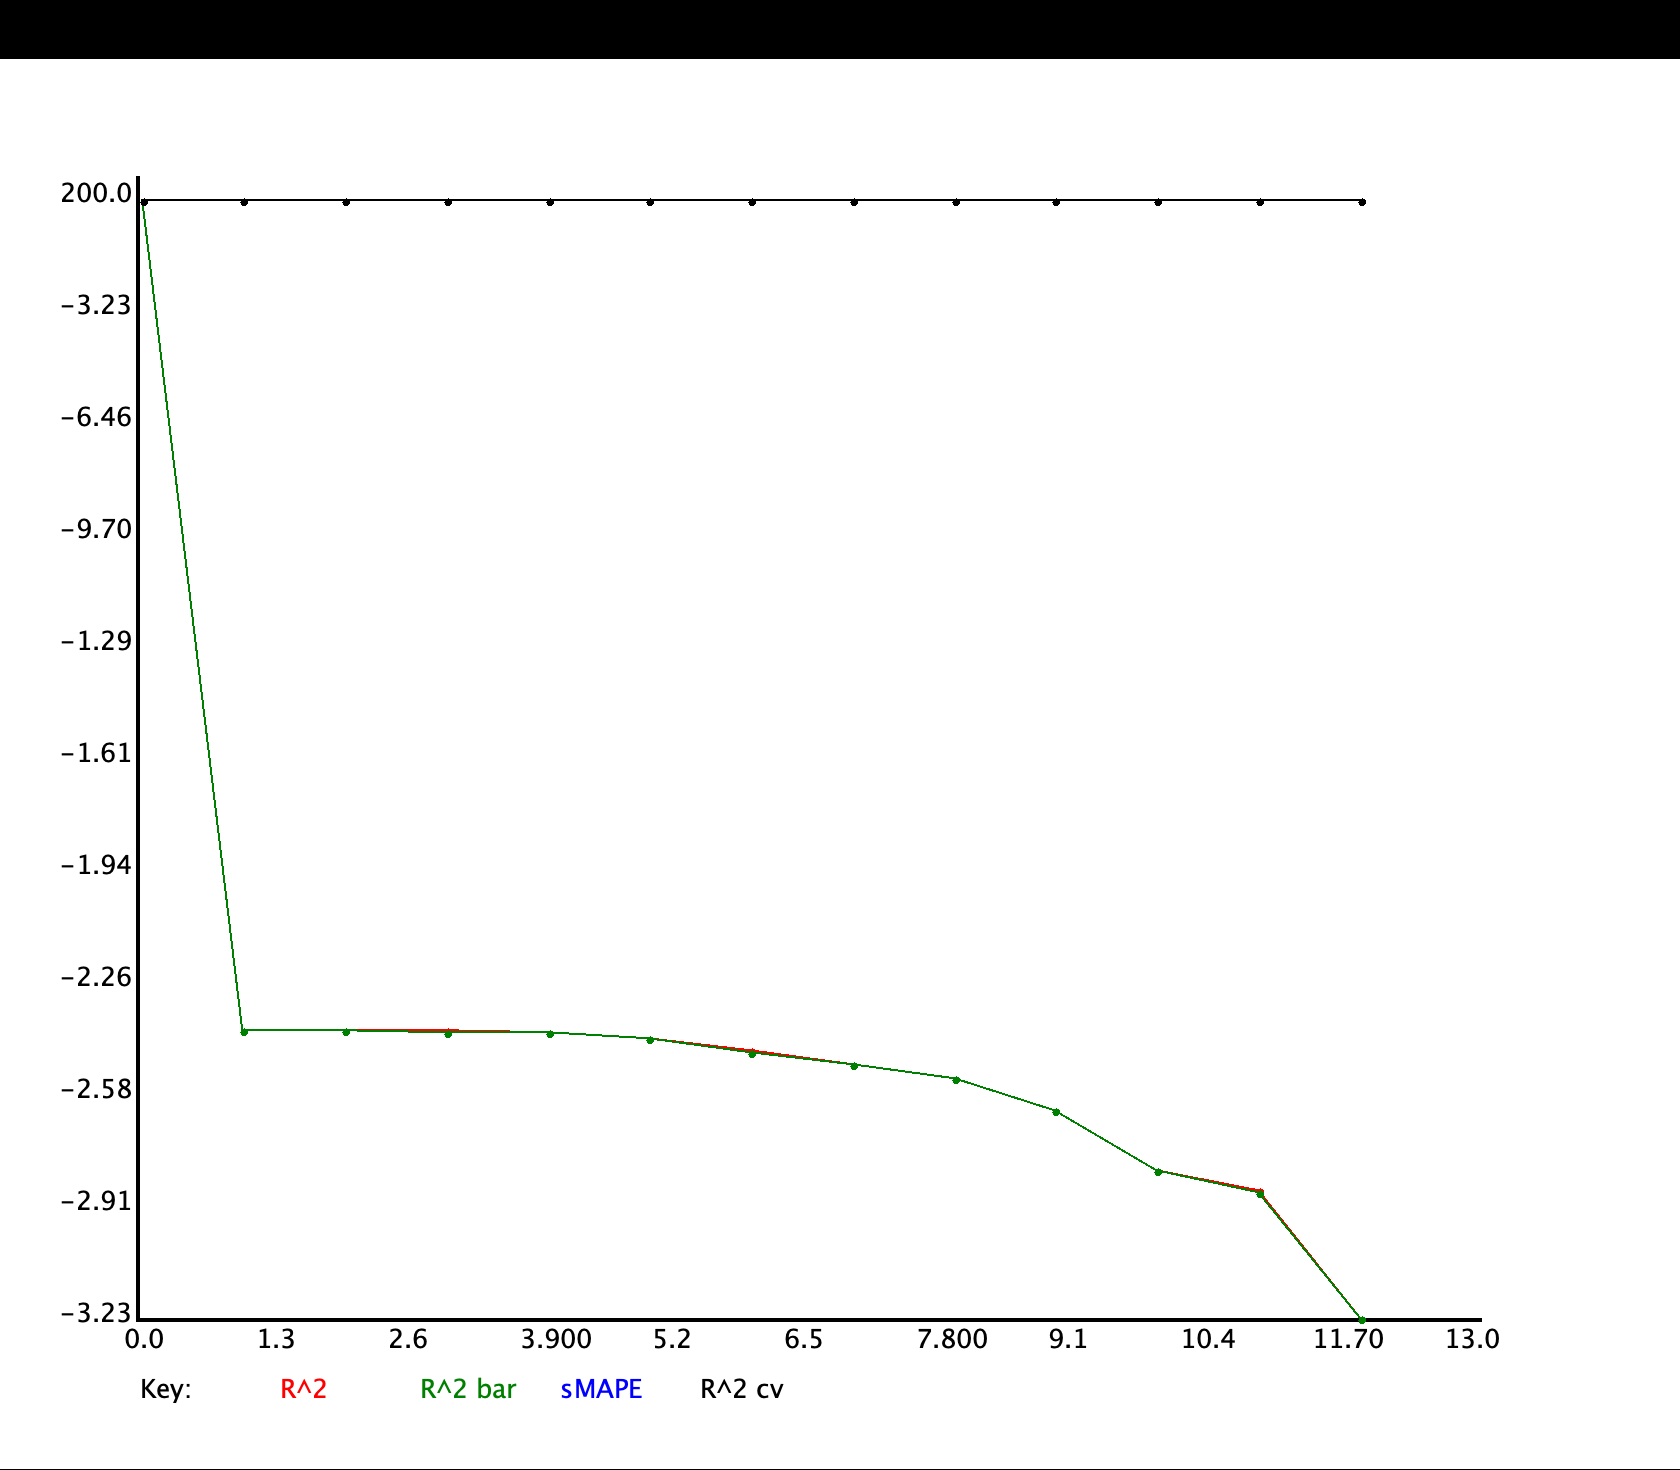
\includegraphics[width=\textwidth]{../House_Prices_Scalation_Plots/Scalation_Sqrt_rSq_Forward.png}
     \end{subfigure}
     \hfill
     \begin{subfigure}[b]{0.4\textwidth}
         \centering
         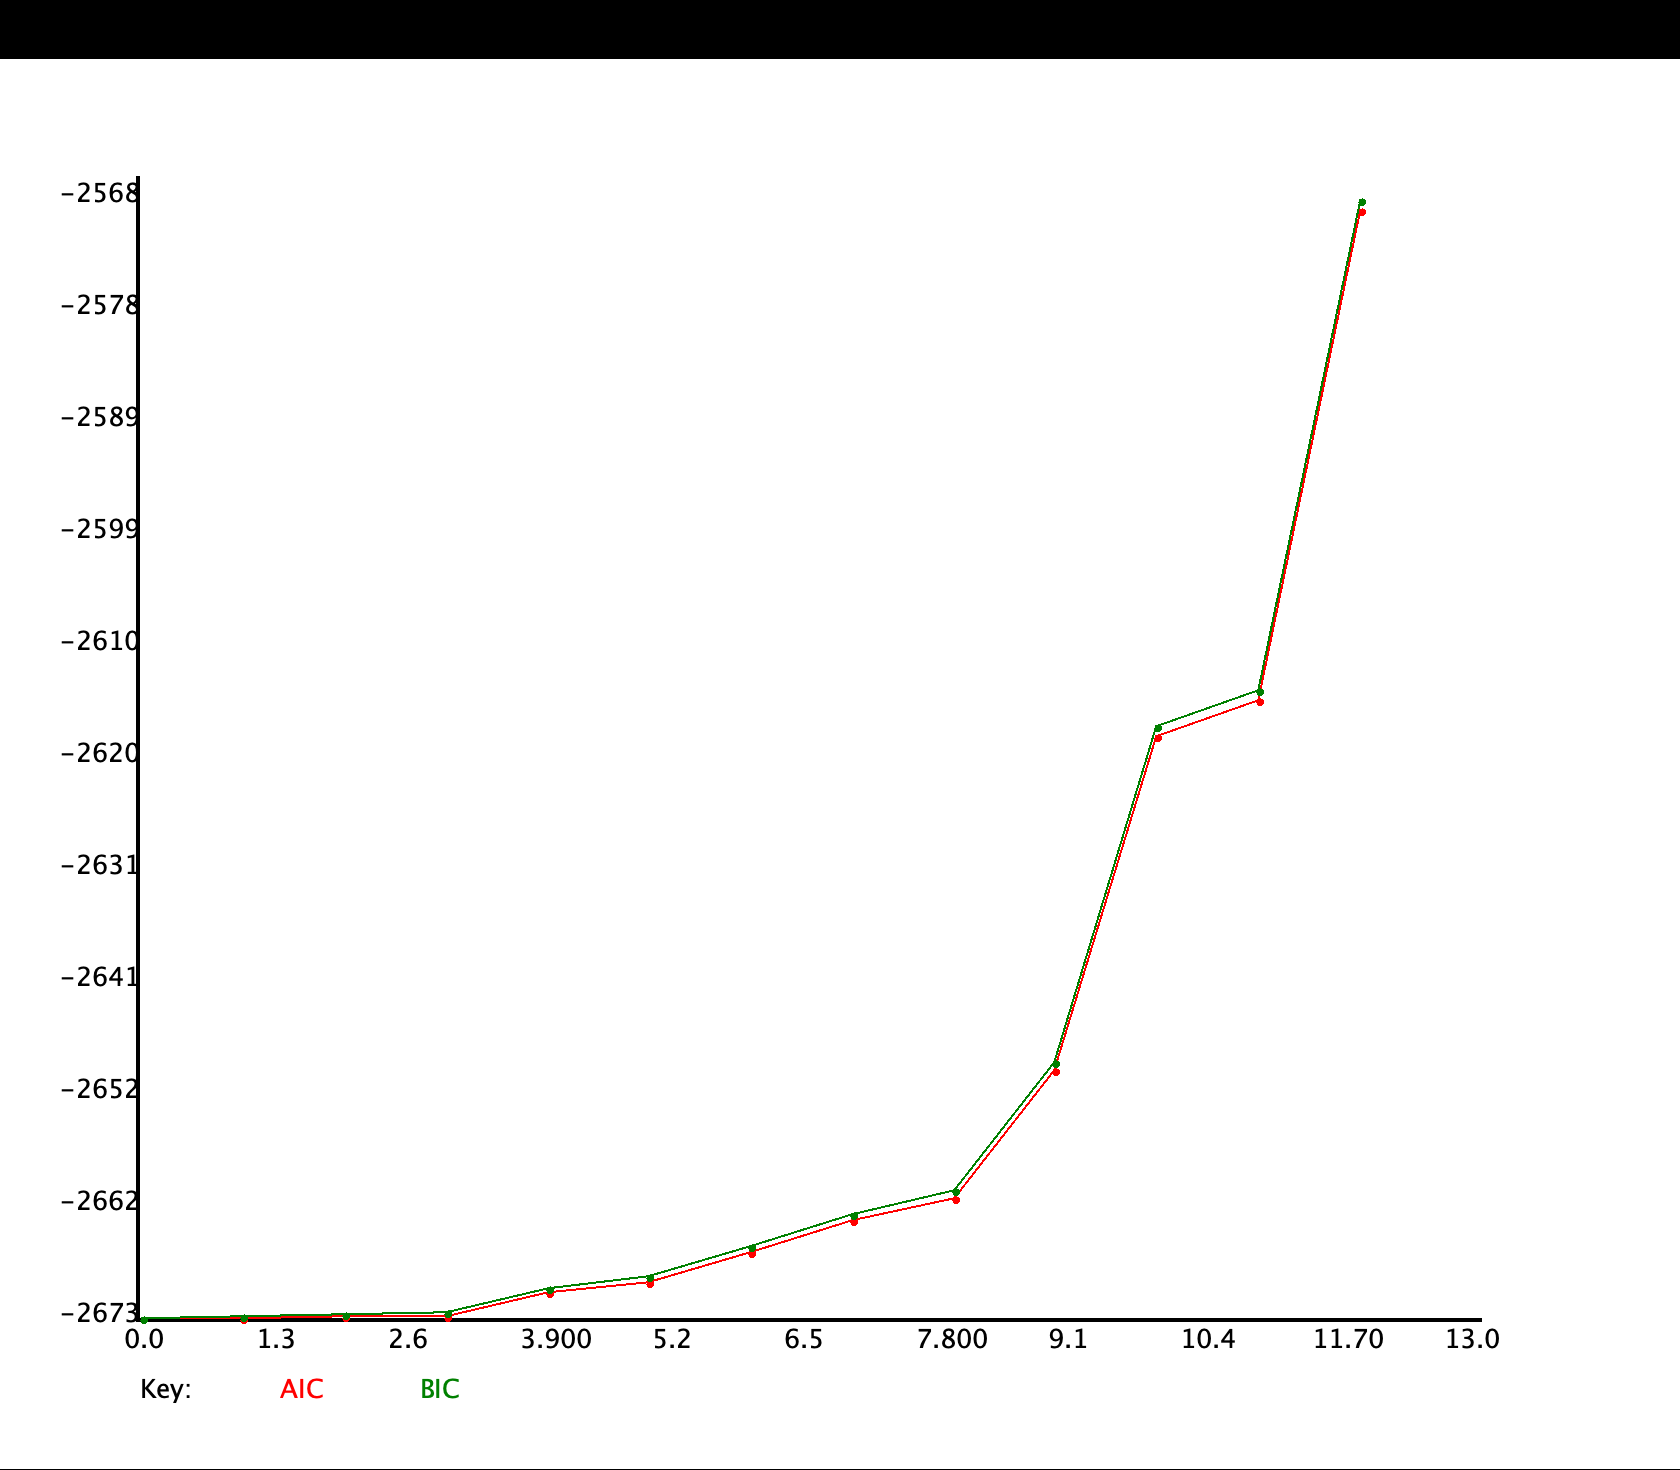
\includegraphics[width=\textwidth]{../House_Prices_Scalation_Plots/Scalation_Sqrt_AIC_BIC_Forward.png}
     \end{subfigure}

     \vspace{10pt} % Add some vertical spacing between rows

     % Second Row
     \begin{subfigure}[b]{0.49\textwidth}
         \centering
         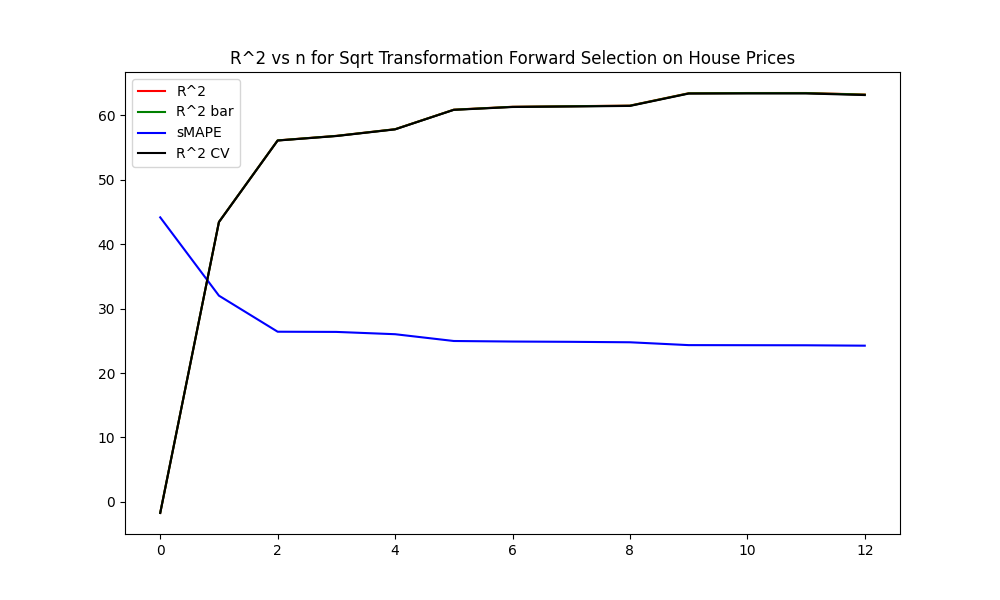
\includegraphics[width=\textwidth]{../House_Prices_Statsmodels_Plots/Statsmodels_Sqrt_rSq_Forward.png}
     \end{subfigure}
     \hfill
     \begin{subfigure}[b]{0.49\textwidth}
         \centering
         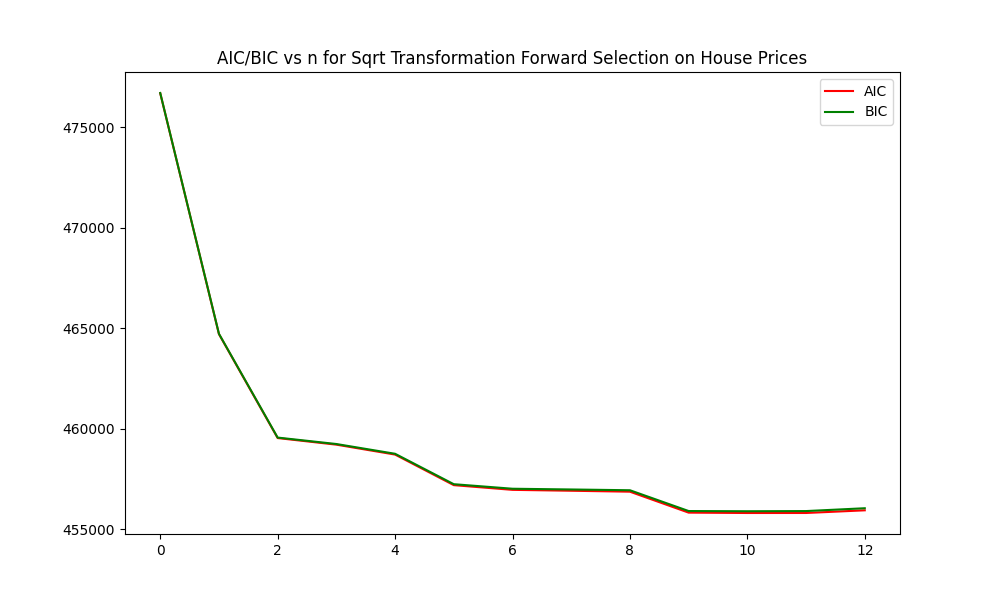
\includegraphics[width=\textwidth]{../House_Prices_Statsmodels_Plots/Statsmodels_Sqrt_AIC_BIC_Forward.png}
     \end{subfigure}
     
     \caption{California House Prices Sqrt Transformation Forward Selection Quality of Fit Metrics\\ Top Left: Scalation $R^2$, Top Right: Scalation AIC/BIC\\ Bottom Left: Statsmodels $R^2$, Bottom Right: Statsmodels AIC/BIC}
     \label{fig:California House Prices Sqrt Transformation Forward Selection Quality of Fit Metrics}
\end{figure}

Scalation Backward Elimination Reversed: intercept, longitude, ocean proximity ISLAND, ocean proximity NEAR OCEAN, total bedrooms, households, housing median age, ocean proximity NEAR BAY, latitude, ocean proximity INLAND, population, total rooms, median income

Statsmodels Backward Elimination Reversed: intercept, median income, latitude, longitude, households, population, housing median age, ocean proximity INLAND, total bedrooms, ocean proximity ISLAND, ocean proximity NEAR BAY, ocean proximity NEAR OCEAN, total rooms

\begin{figure}[H]
     \centering
     \captionsetup{justification=centering}
     % First Row
     \begin{subfigure}[b]{0.4\textwidth}
         \centering
         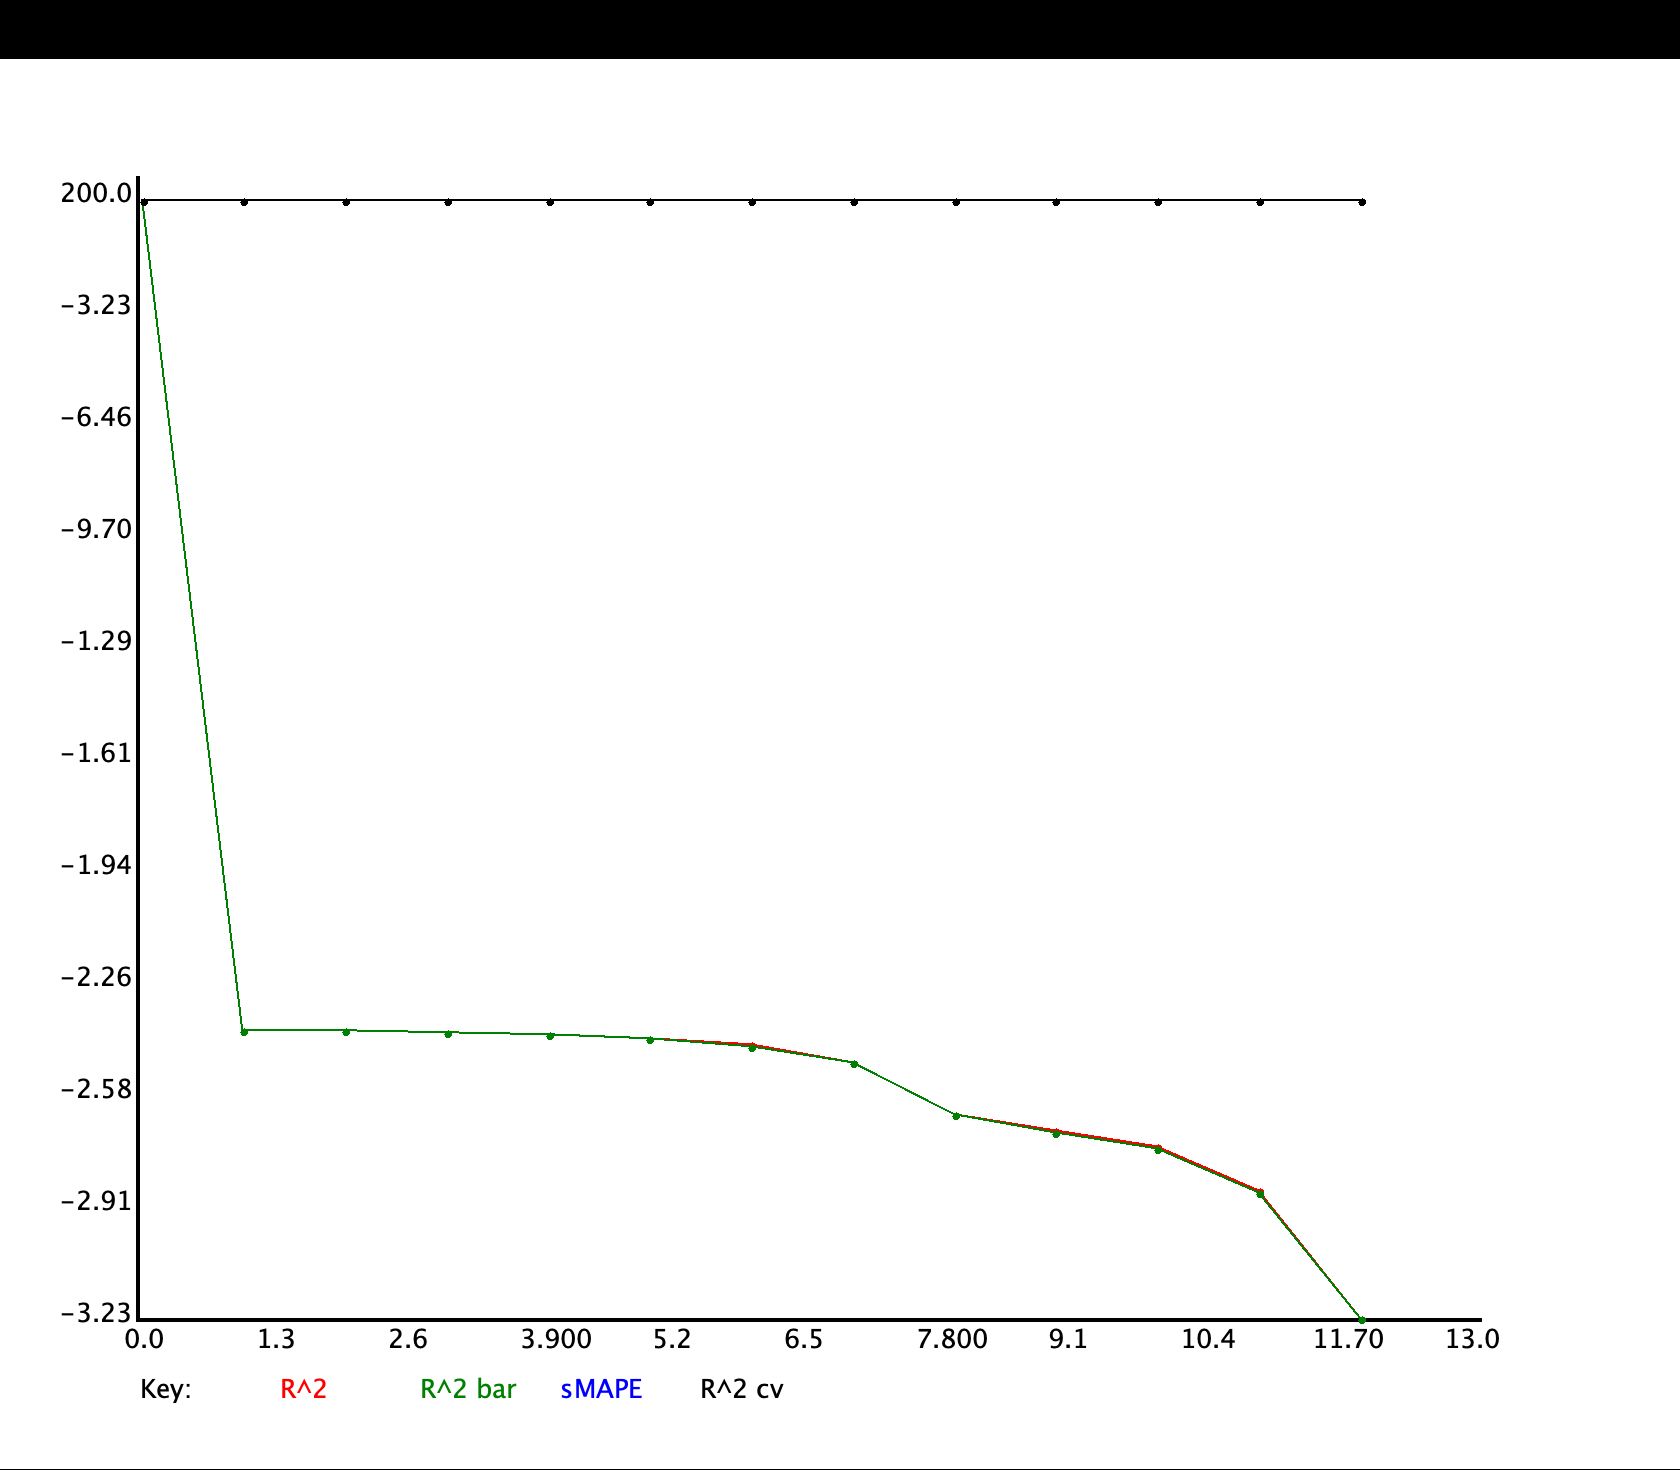
\includegraphics[width=\textwidth]{../House_Prices_Scalation_Plots/Scalation_Sqrt_rSq_Backward.png}
     \end{subfigure}
     \hfill
     \begin{subfigure}[b]{0.4\textwidth}
         \centering
         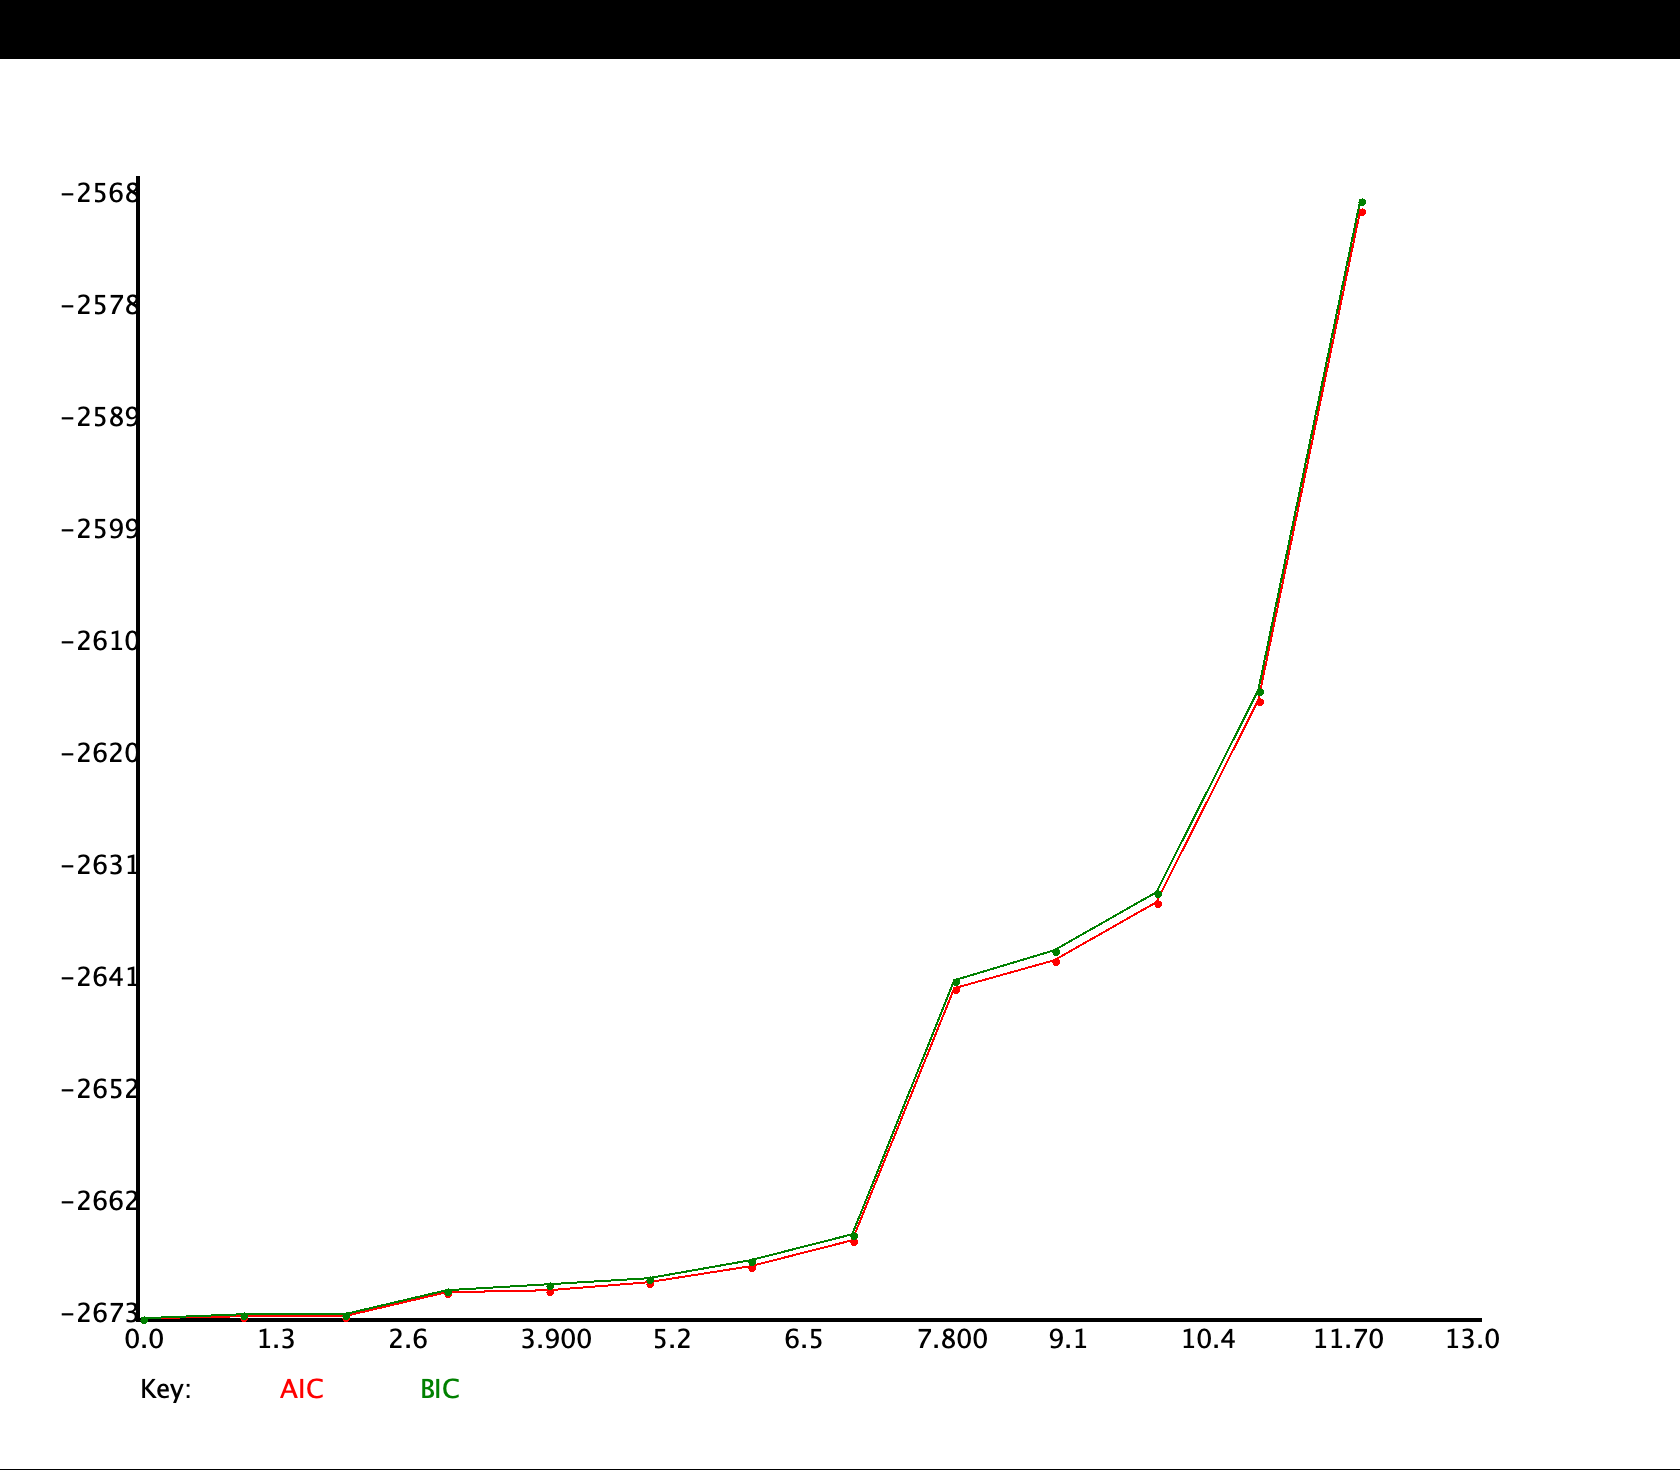
\includegraphics[width=\textwidth]{../House_Prices_Scalation_Plots/Scalation_Sqrt_AIC_BIC_Backward.png}
     \end{subfigure}

     \vspace{10pt} % Add some vertical spacing between rows

     % Second Row
     \begin{subfigure}[b]{0.49\textwidth}
         \centering
         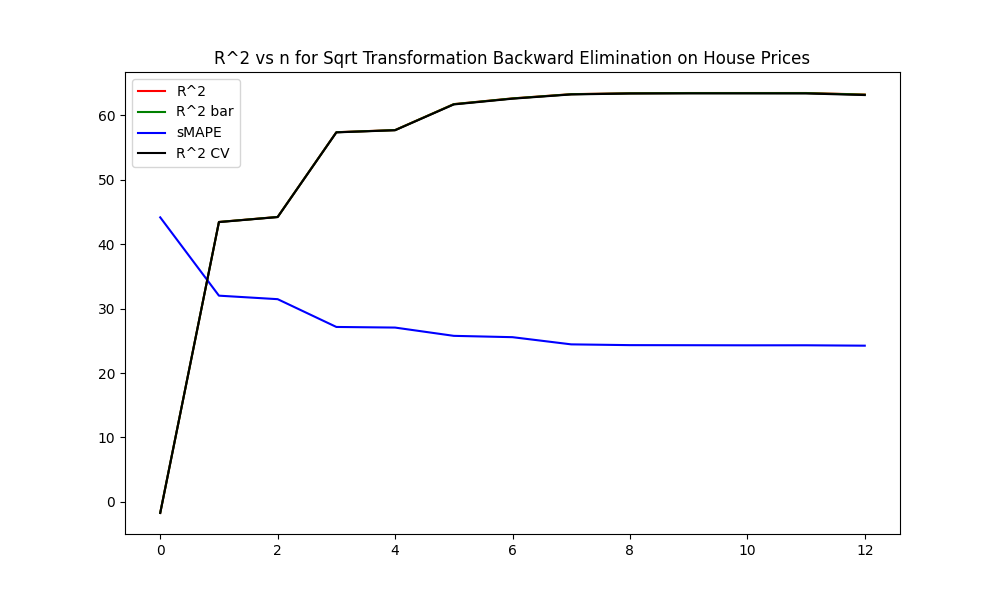
\includegraphics[width=\textwidth]{../House_Prices_Statsmodels_Plots/Statsmodels_Sqrt_rSq_Backward.png}
     \end{subfigure}
     \hfill
     \begin{subfigure}[b]{0.49\textwidth}
         \centering
         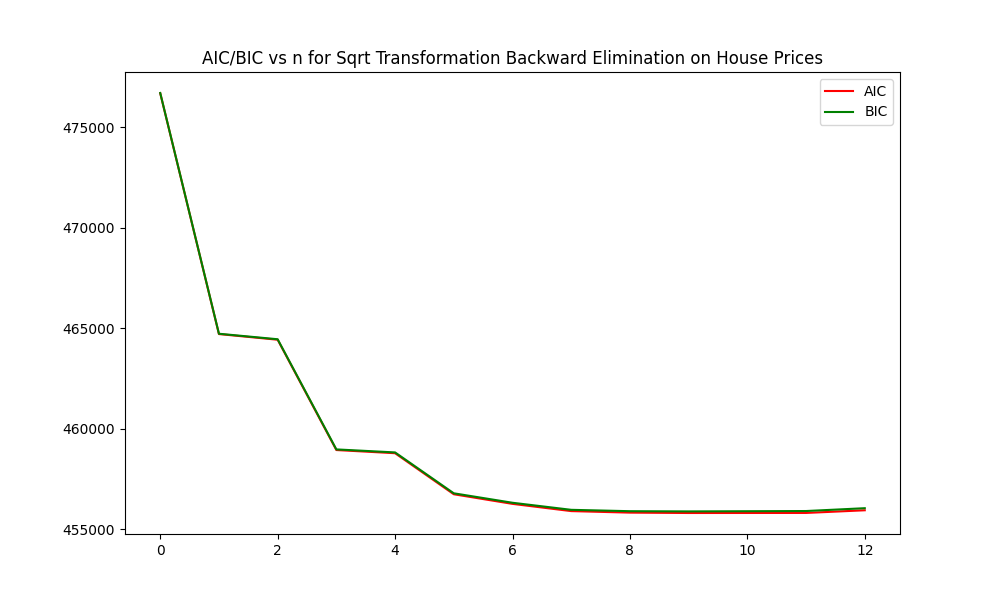
\includegraphics[width=\textwidth]{../House_Prices_Statsmodels_Plots/Statsmodels_Sqrt_AIC_BIC_Backward.png}
     \end{subfigure}
     
     \caption{California House Prices Sqrt Transformation Reversed Backward Elimination Quality of Fit Metrics\\ Top Left: Scalation $R^2$, Top Right: Scalation AIC/BIC\\ Bottom Left: Statsmodels $R^2$, Bottom Right: Statsmodels AIC/BIC}
     \label{fig:California House Prices Sqrt Transformation Reversed Backward Elimination Quality of Fit Metrics}
\end{figure}

Scalation Stepwise Selection: intercept

Statsmodels Stepwise Selection: intercept, median income, ocean proximity INLAND, housing median age, total bedrooms, population, households, longitude, latitude, ocean proximity ISLAND

\begin{figure}[H]
     \centering
     \captionsetup{justification=centering}
%     % First Row
%     \begin{subfigure}[b]{0.4\textwidth}
%         \centering
%         %\includegraphics[width=\textwidth]{../House_Prices_Scalation_Plots/Scalation_Sqrt_rSq_Stepwise.png}
%     \end{subfigure}
%     \hfill
%     \begin{subfigure}[b]{0.4\textwidth}
%         \centering
%         %\includegraphics[width=\textwidth]{../House_Prices_Scalation_Plots/Scalation_Sqrt_AIC_BIC_Stepwise.png}
%     \end{subfigure}
%
%     \vspace{10pt} % Add some vertical spacing between rows

     % Second Row
     \begin{subfigure}[b]{0.49\textwidth}
         \centering
         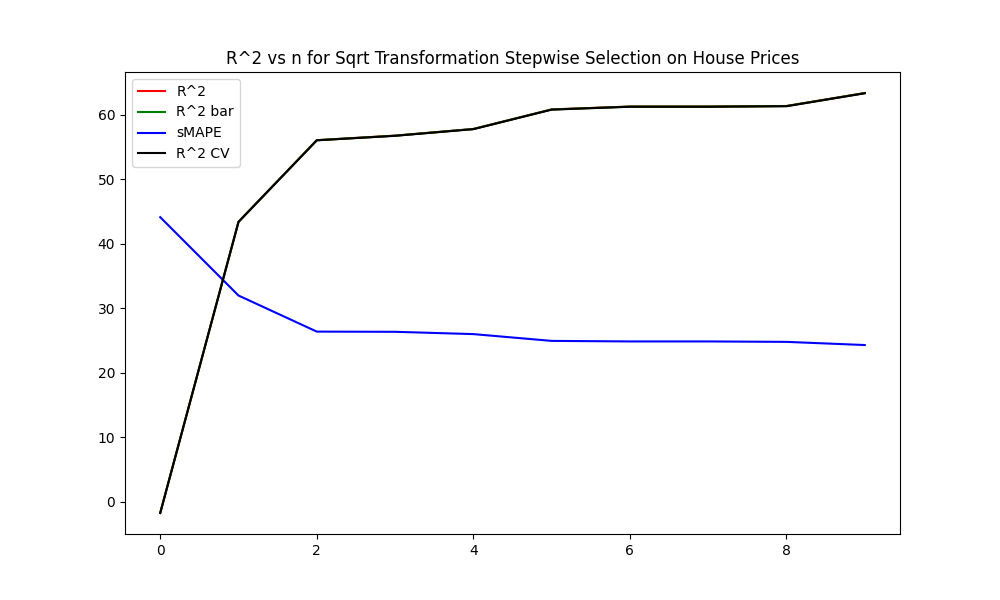
\includegraphics[width=\textwidth]{../House_Prices_Statsmodels_Plots/Statsmodels_Sqrt_rSq_Stepwise.png}
     \end{subfigure}
     \hfill
     \begin{subfigure}[b]{0.49\textwidth}
         \centering
         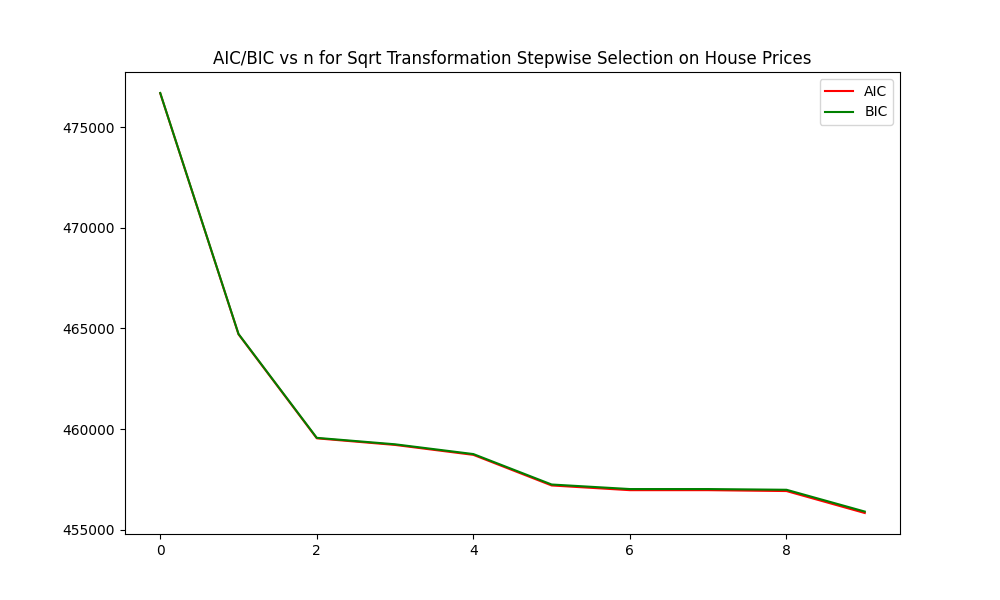
\includegraphics[width=\textwidth]{../House_Prices_Statsmodels_Plots/Statsmodels_Sqrt_AIC_BIC_Stepwise.png}
     \end{subfigure}
     
     \caption{California House Prices Sqrt Transformation Stepwise Selection Quality of Fit Metrics\\ Left: Statsmodels $R^2$, Right: Statsmodels AIC/BIC}
     \label{fig:California House Prices Sqrt Transformation Stepwise Selection Quality of Fit Metrics}
\end{figure}

\subsection{Log1p Transformation}

\subsubsection{Quality of Fit}

\begin{table}[H]
\centering
\caption{Scalation - California House Prices Log1p Transformation}
\label{tab:Scalation - House Prices Log1p Transformation}
\begin{tabular}{|c|c|c|} \hline 
Metric & In-Sample & 80-20 Split \\ \hline \hline 
rSq &0.433647 & 0.385506 \\ \hline 
rSqBar &0.433314 &      0.385144 \\ \hline 
sst &2.72264e+14 &      5.31945e+13 \\ \hline 
sse &1.54198e+14 &      3.26877e+13 \\ \hline 
sde &86513.6 &  89289.8 \\ \hline 
mse0 &7.54651e+09 &     7.99993e+09 \\ \hline 
rmse &86870.6 & 89442.3 \\ \hline 
mae &51134.7 &  50841.2 \\ \hline 
smape &24.3617 &        24.3176 \\ \hline 
m &20433.0 &    4086.00 \\ \hline 
dfr &12.0000 &  12.0000 \\ \hline 
df &20420.0 &   20420.0 \\ \hline 
fStat &1302.94 &        1067.55 \\ \hline 
aic &-261335 &  -52357.7 \\ \hline 
bic &-261232 &  -52275.6 \\ \hline 
\end{tabular}
\end{table}

\begin{table}[H]
\centering
\caption{Statsmodels - California House Prices Log1p Transformation}
\label{tab:Statsmodels - House Prices Log1p Transformation}
\begin{tabular}{|c|c|c|}\hline
Metric & In-Sample & 80-20 Split \\ \hline \hline
rSq & 0.6654 & 0.4737 \\ \hline
rSqBar & 0.6652 & 0.4722 \\ \hline
sst & 6620.1593 & 54723646809444.8438 \\ \hline
sse & 2214.8654 & 28799287585802.4219 \\ \hline
sde & 0.3293 & 84077.6104 \\ \hline
mse0 & 0.1085 & 7046559233.1300 \\ \hline
rmse & 0.3293 & 83943.7861 \\ \hline
mae & 51134.7092 & 50653.6747 \\ \hline
smape & 24.3617 & 24.2321 \\ \hline
m & 20433.0000 & 4087.0000 \\ \hline
dfr & 12.0000 & 13.0000 \\ \hline
df & 20420.0000 & 4074.0000 \\ \hline
fStat & 3384.5587 & 282.1006 \\ \hline
aic & 12611.0413 & 92702.0162 \\ \hline
bic & 12714.0651 & 92784.1186 \\ \hline
\end{tabular}
\end{table}

\begin{table}[H]
\centering
\caption{Scalation - California House Prices Log1p Transformation CV}
\label{tab:Scalation - House Prices Log1p Transformation CV}
\begin{tabular}{|c|c|c|c|c|c|}\hline
Metric & num folds & min & max & mean & stdev \\ \hline \hline
rSq & 5 & 0.259 & 0.543 & 0.428 & 0.112 \\ \hline
rSqBar & 5 & 0.259 & 0.542 & 0.427 & 0.112 \\ \hline
sst & 5 & 53194492241132.980 & 57310203956796.625 & 54411355017051.000 & 1675890609056.710 \\ \hline
sse & 5 & 24631652267892.707 & 42455602670672.420 & 31254784480308.344 & 6957091932106.546 \\ \hline
sde & 5 & 77093.724 & 101586.791 & 86695.562 & 9497.720 \\ \hline
mse0 & 5 & 6028304519.798 & 10390504814.164 & 7649237513.536 & 1702665671.098 \\ \hline
rmse & 5 & 77642.157 & 101933.826 & 87052.332 & 9429.282 \\ \hline
mae & 5 & 49720.736 & 56073.033 & 51242.091 & 2740.865 \\ \hline
smape & 5 & 23.784 & 24.873 & 24.388 & 0.413 \\ \hline
m & 5 & 4086.000 & 4086.000 & 4086.000 & 0.000 \\ \hline
dfr & 5 & 12.000 & 12.000 & 12.000 & 0.000 \\ \hline
df & 5 & 20420.000 & 20420.000 & 20420.000 & 0.000 \\ \hline
fStat & 5 & 595.389 & 2017.945 & 1357.095 & 559.408 \\ \hline
aic & 5 & -52970.445 & -51852.356 & -52267.823 & 436.415 \\ \hline
bic & 5 & -52888.346 & -51770.257 & -52185.724 & 436.415 \\ \hline
\end{tabular}
\end{table}

\begin{table}[H]
\centering
\caption{Statsmodels - California House Prices Log1p Transformation CV}
\label{tab:Statsmodels - House Prices Log1p Transformation CV}
\begin{tabular}{|c|c|c|c|c|c|}\hline
Metric & num folds & min & max & mean & stdev \\ \hline \hline
rSq & 5 & 0.3590 & 0.4841 & 0.4316 & 0.0449 \\ \hline
rSqBar & 5 & 0.3571 & 0.4826 & 0.4300 & 0.0451 \\ \hline
sst & 5 & 53541750406767.3438 & 54912923487891.5781 & 54447676367709.7031 & 499826929365.4288 \\ \hline
sse & 5 & 28330032199007.3672 & 34795616267062.3281 & 30933456233892.7578 & 2308307378030.6714 \\ \hline
sde & 5 & 83389.8172 & 92428.3204 & 87081.9059 & 3230.1438 \\ \hline
mse0 & 5 & 6931742647.1758 & 8515814064.3814 & 7569535497.0312 & 565550107.7130 \\ \hline
rmse & 5 & 83257.0877 & 92281.1685 & 86943.2858 & 3224.9893 \\ \hline
mae & 5 & 49955.0821 & 52692.3412 & 51184.1437 & 906.5915 \\ \hline
smape & 5 & 23.9545 & 24.7523 & 24.3785 & 0.2792 \\ \hline
m & 5 & 4086.0000 & 4087.0000 & 4086.6000 & 0.4899 \\ \hline
dfr & 5 & 13.0000 & 13.0000 & 13.0000 & 0.0000 \\ \hline
df & 5 & 4073.0000 & 4074.0000 & 4073.6000 & 0.4899 \\ \hline
fStat & 5 & 175.4670 & 294.0579 & 241.3681 & 42.9122 \\ \hline
aic & 5 & 92634.8741 & 93453.1694 & 92974.3014 & 292.6689 \\ \hline
bic & 5 & 92716.9765 & 93535.2686 & 93056.4025 & 292.6677 \\ \hline
\end{tabular}
\end{table}

\begin{figure}[H]
     \centering
     \captionsetup{justification=centering}
     % First Row
     \begin{subfigure}[b]{0.4\textwidth}
         \centering
         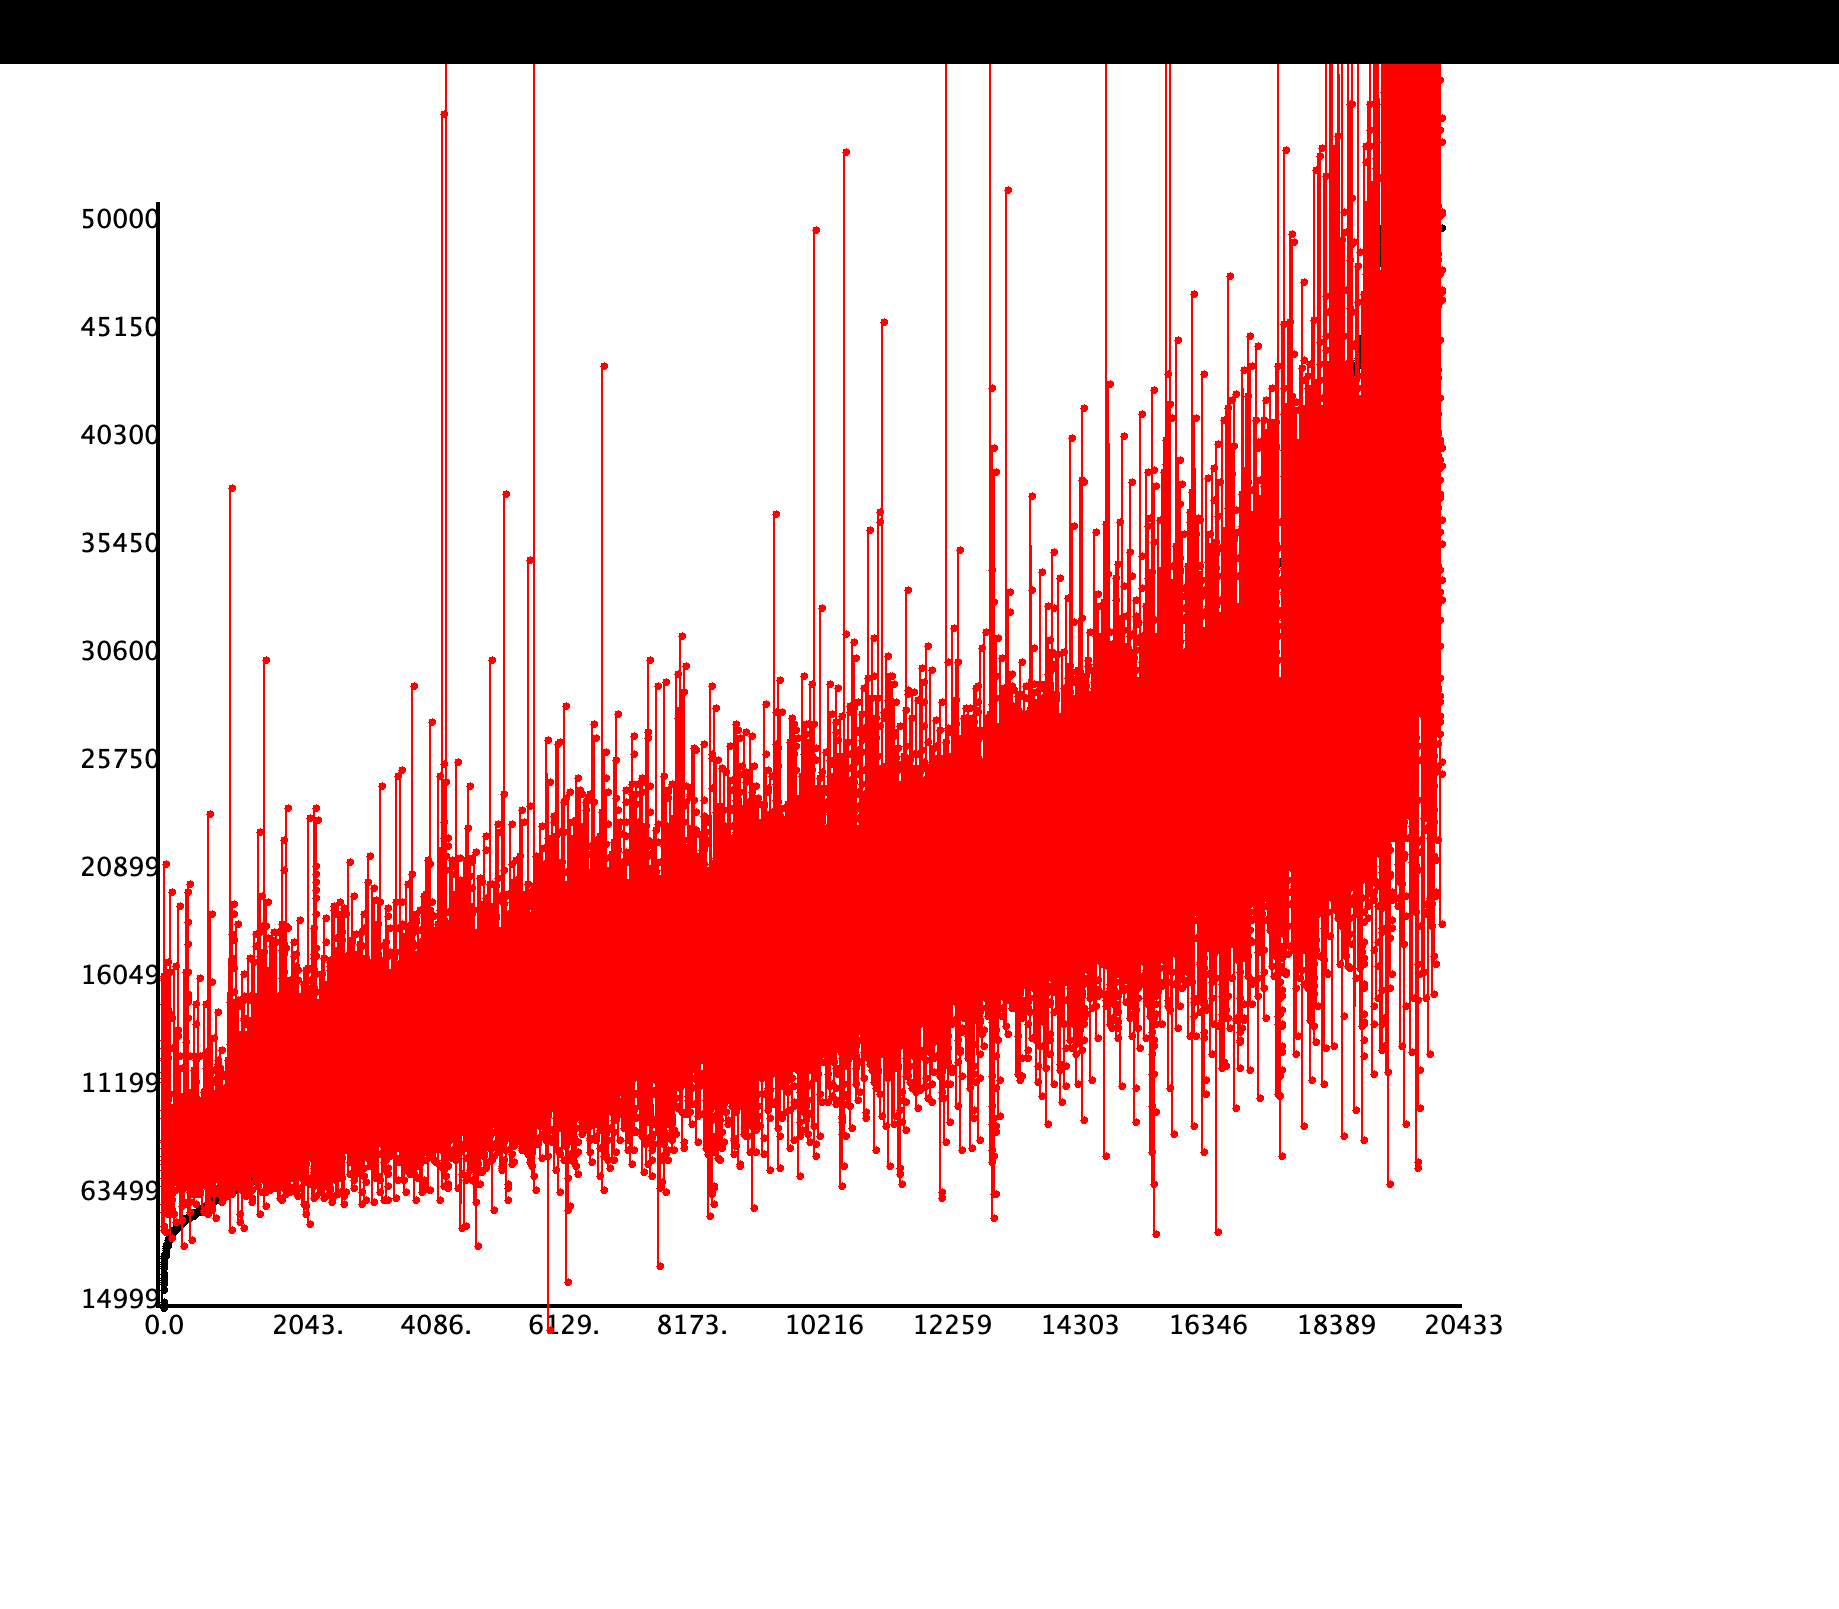
\includegraphics[width=\textwidth]{../House_Prices_Scalation_Plots/Scalation_Log1p_In_Sample.png}
     \end{subfigure}
     \hfill
     \begin{subfigure}[b]{0.4\textwidth}
         \centering
         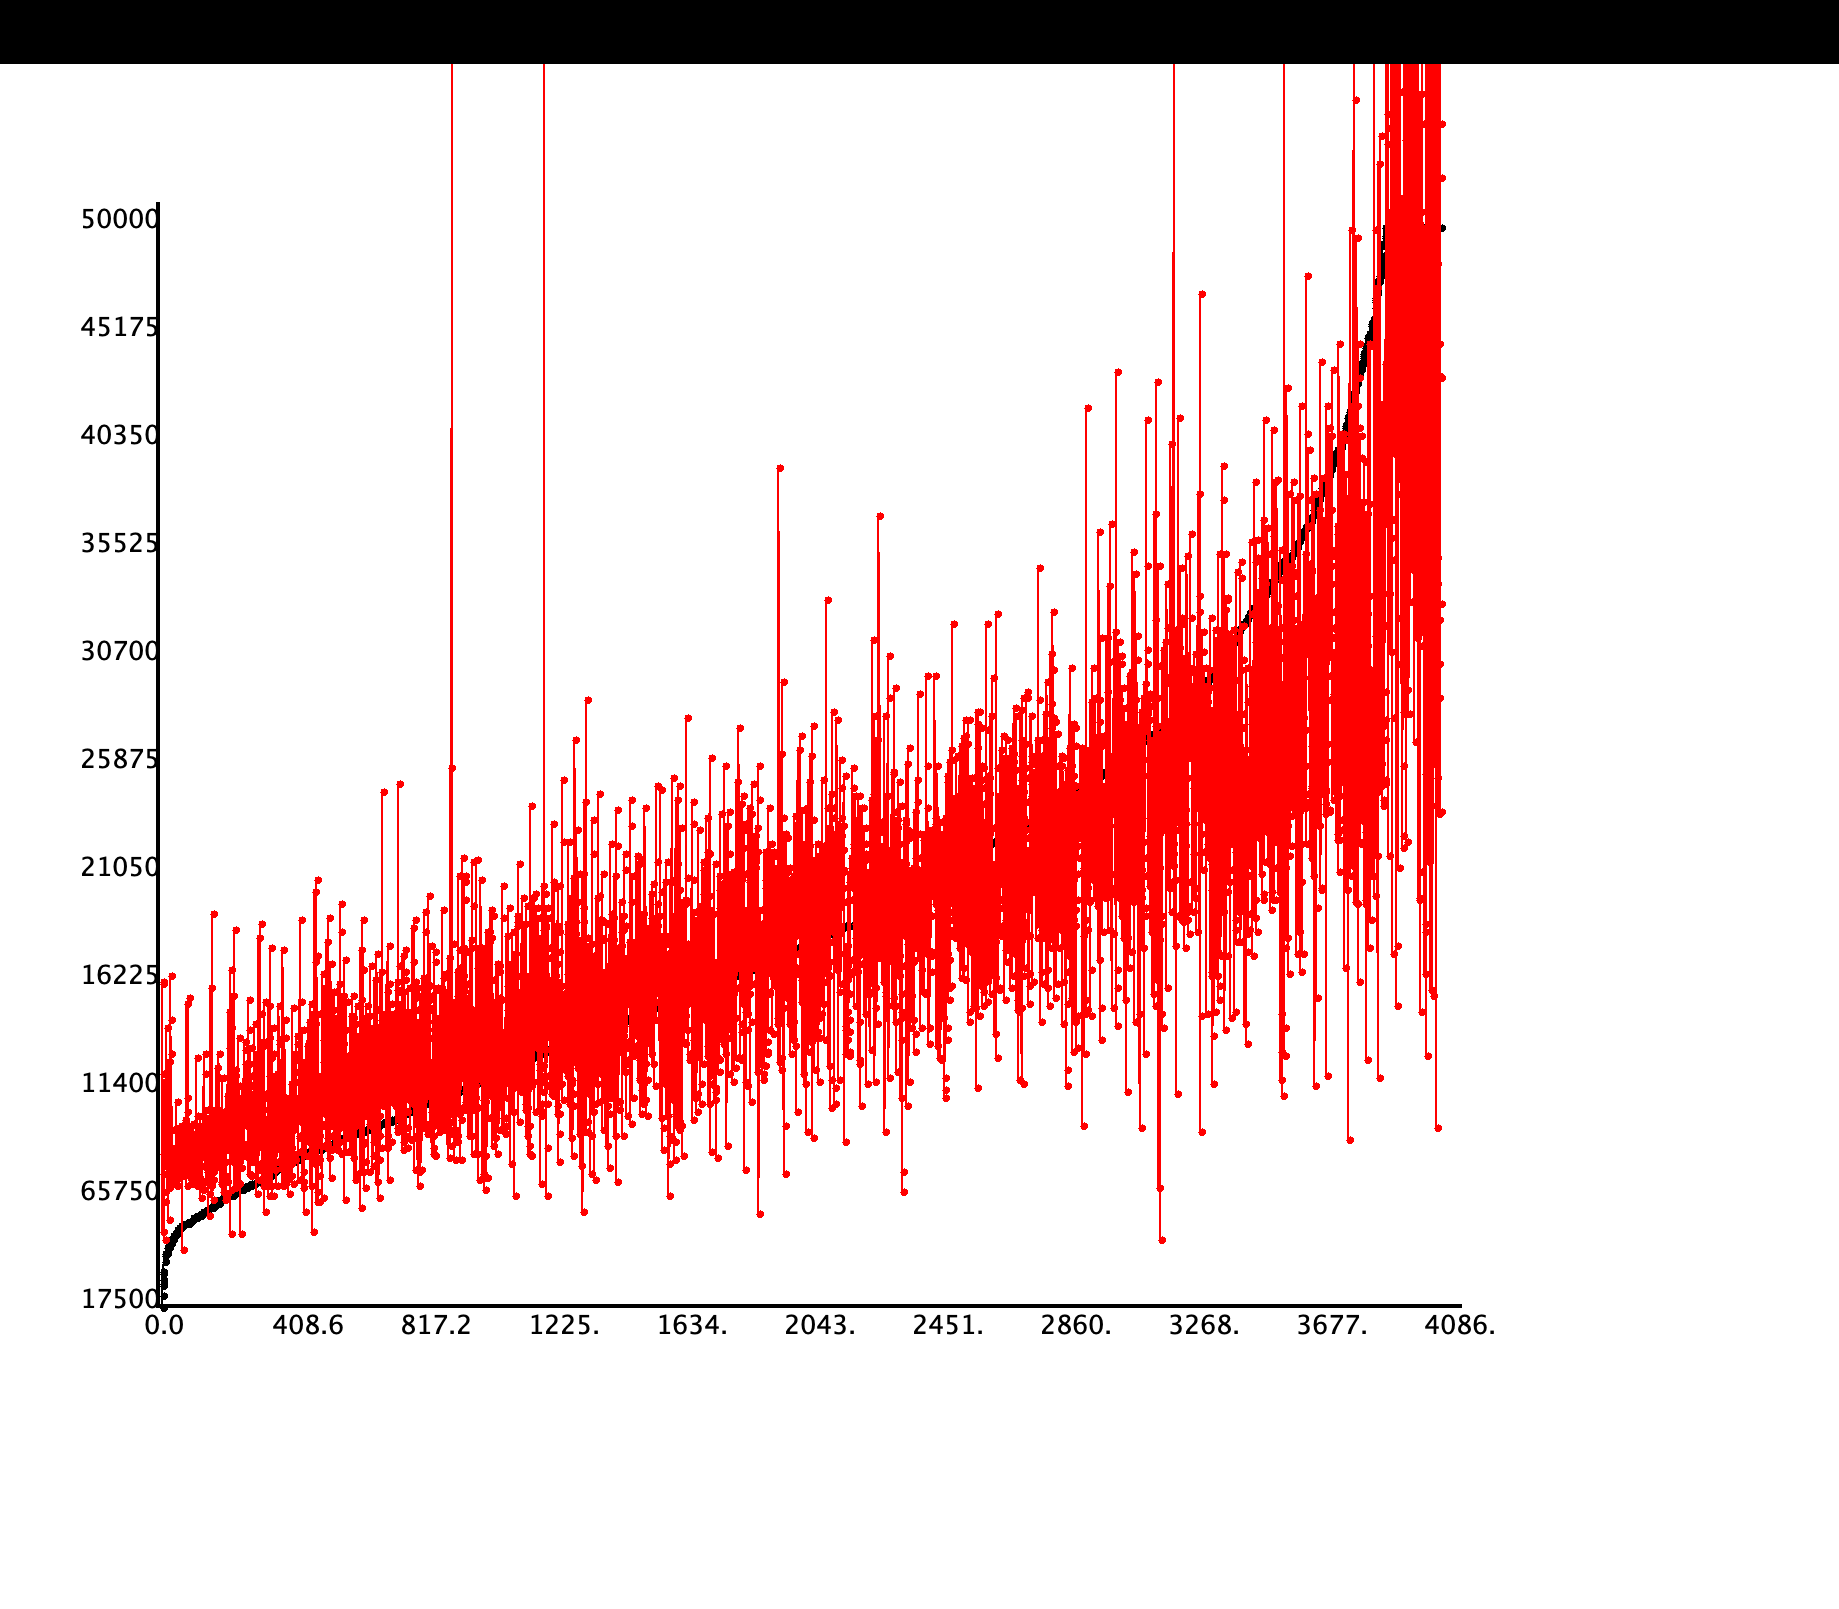
\includegraphics[width=\textwidth]{../House_Prices_Scalation_Plots/Scalation_Log1p_80_20.png}
     \end{subfigure}

     \vspace{10pt} % Add some vertical spacing between rows

     % Second Row
     \begin{subfigure}[b]{0.49\textwidth}
         \centering
         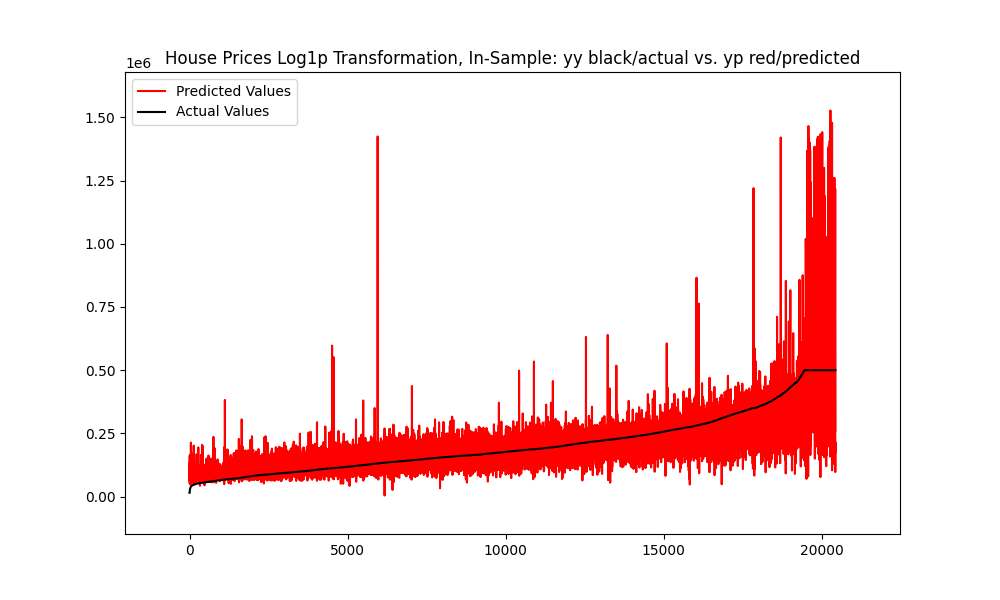
\includegraphics[width=\textwidth]{../House_Prices_Statsmodels_Plots/Statsmodels_Log1p_In_Sample.png}
     \end{subfigure}
     \hfill
     \begin{subfigure}[b]{0.49\textwidth}
         \centering
         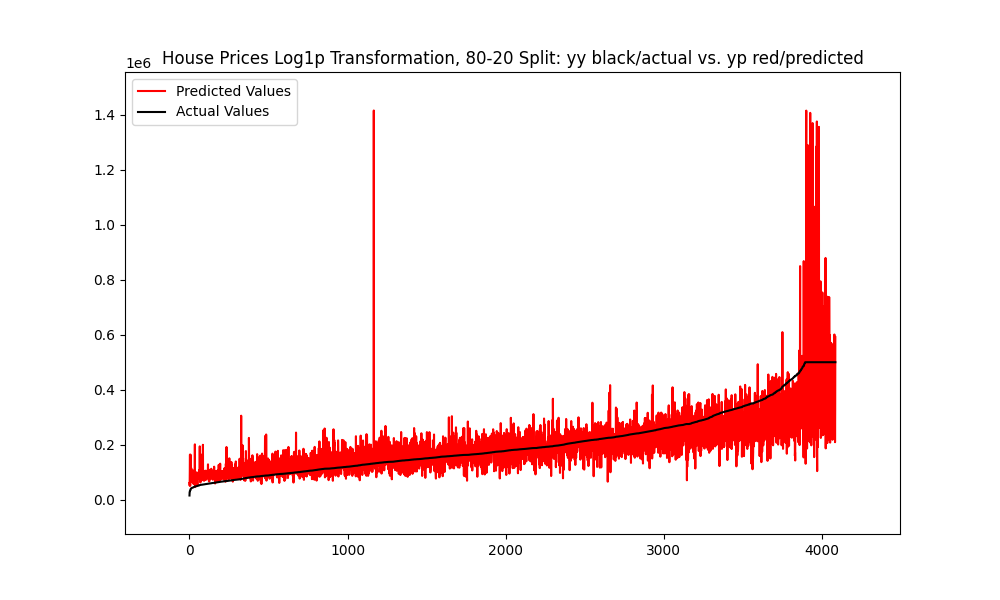
\includegraphics[width=\textwidth]{../House_Prices_Statsmodels_Plots/Statsmodels_Log1p_80_20.png}
     \end{subfigure}
     
     \caption{California House Prices Log1p Transformation Plots\\ Top Left: Scalation In-Sample, Top Right: Scalation Out-of-Sample\\ Bottom Left: Statsmodels In-Sample, Bottom Right: Statsmodels Out-of-Sample\\ black: actual y-values, red: predicted y-values}
     \label{fig:California House Prices Log1p Transformation Plots}
\end{figure}

\subsubsection{Feature Selection}

Scalation Forward Selection: intercept, population, ocean proximity ISLAND, longitude, ocean proximity NEAR OCEAN, housing median age, total bedrooms, households, ocean proximity NEAR BAY, total rooms, latitude, ocean proximity INLAND, median income

Statsmodels Forward Selection: intercept, ocean proximity INLAND, median income, total rooms, population, longitude, latitude, ocean proximity NEAR OCEAN, ocean proximity ISLAND, ocean proximity NEAR BAY, housing median age, households, total bedrooms

\begin{figure}[H]
     \centering
     \captionsetup{justification=centering}
     % First Row
     \begin{subfigure}[b]{0.4\textwidth}
         \centering
         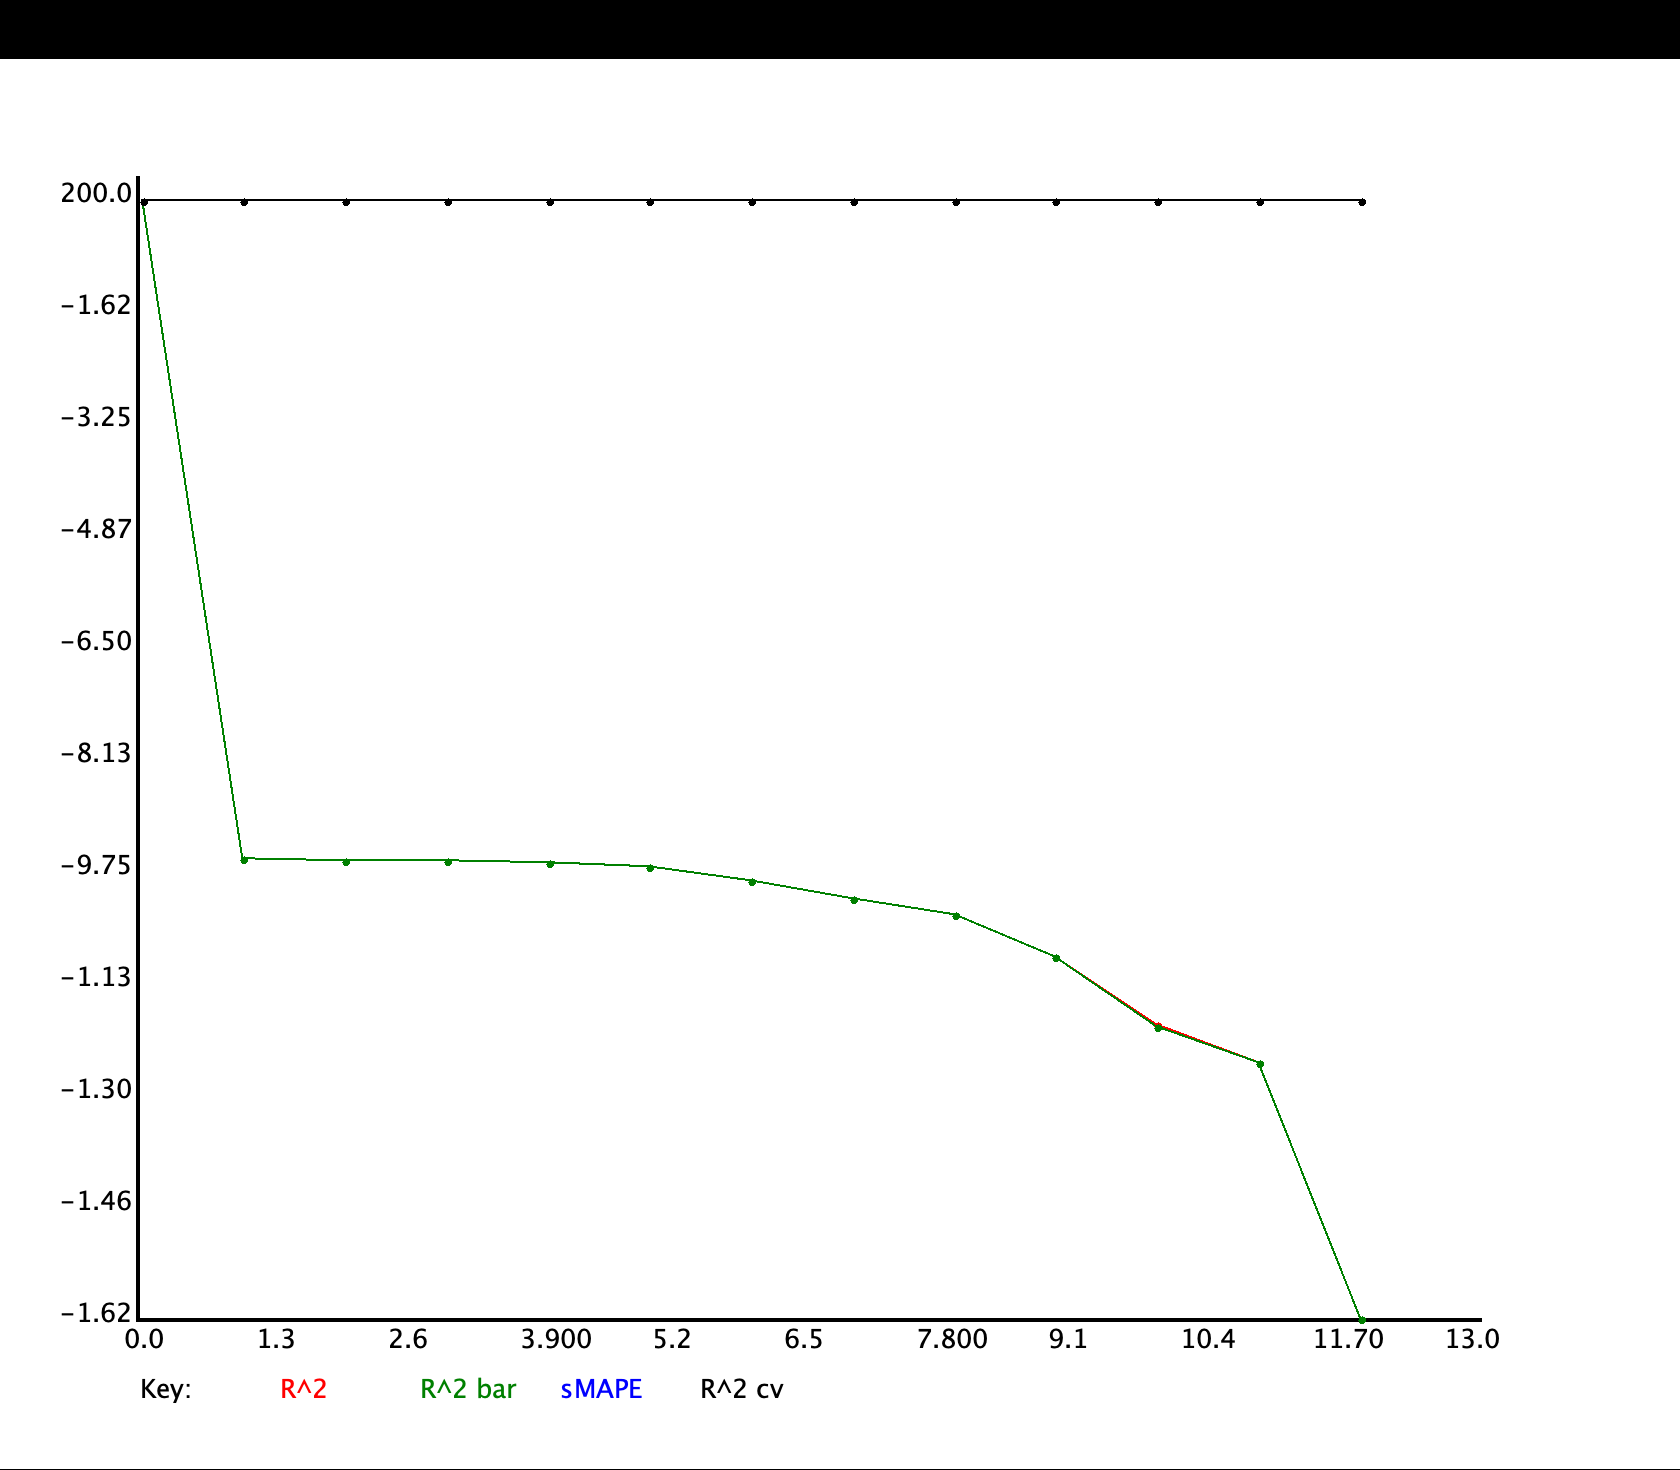
\includegraphics[width=\textwidth]{../House_Prices_Scalation_Plots/Scalation_Log1p_rSq_Forward.png}
     \end{subfigure}
     \hfill
     \begin{subfigure}[b]{0.4\textwidth}
         \centering
         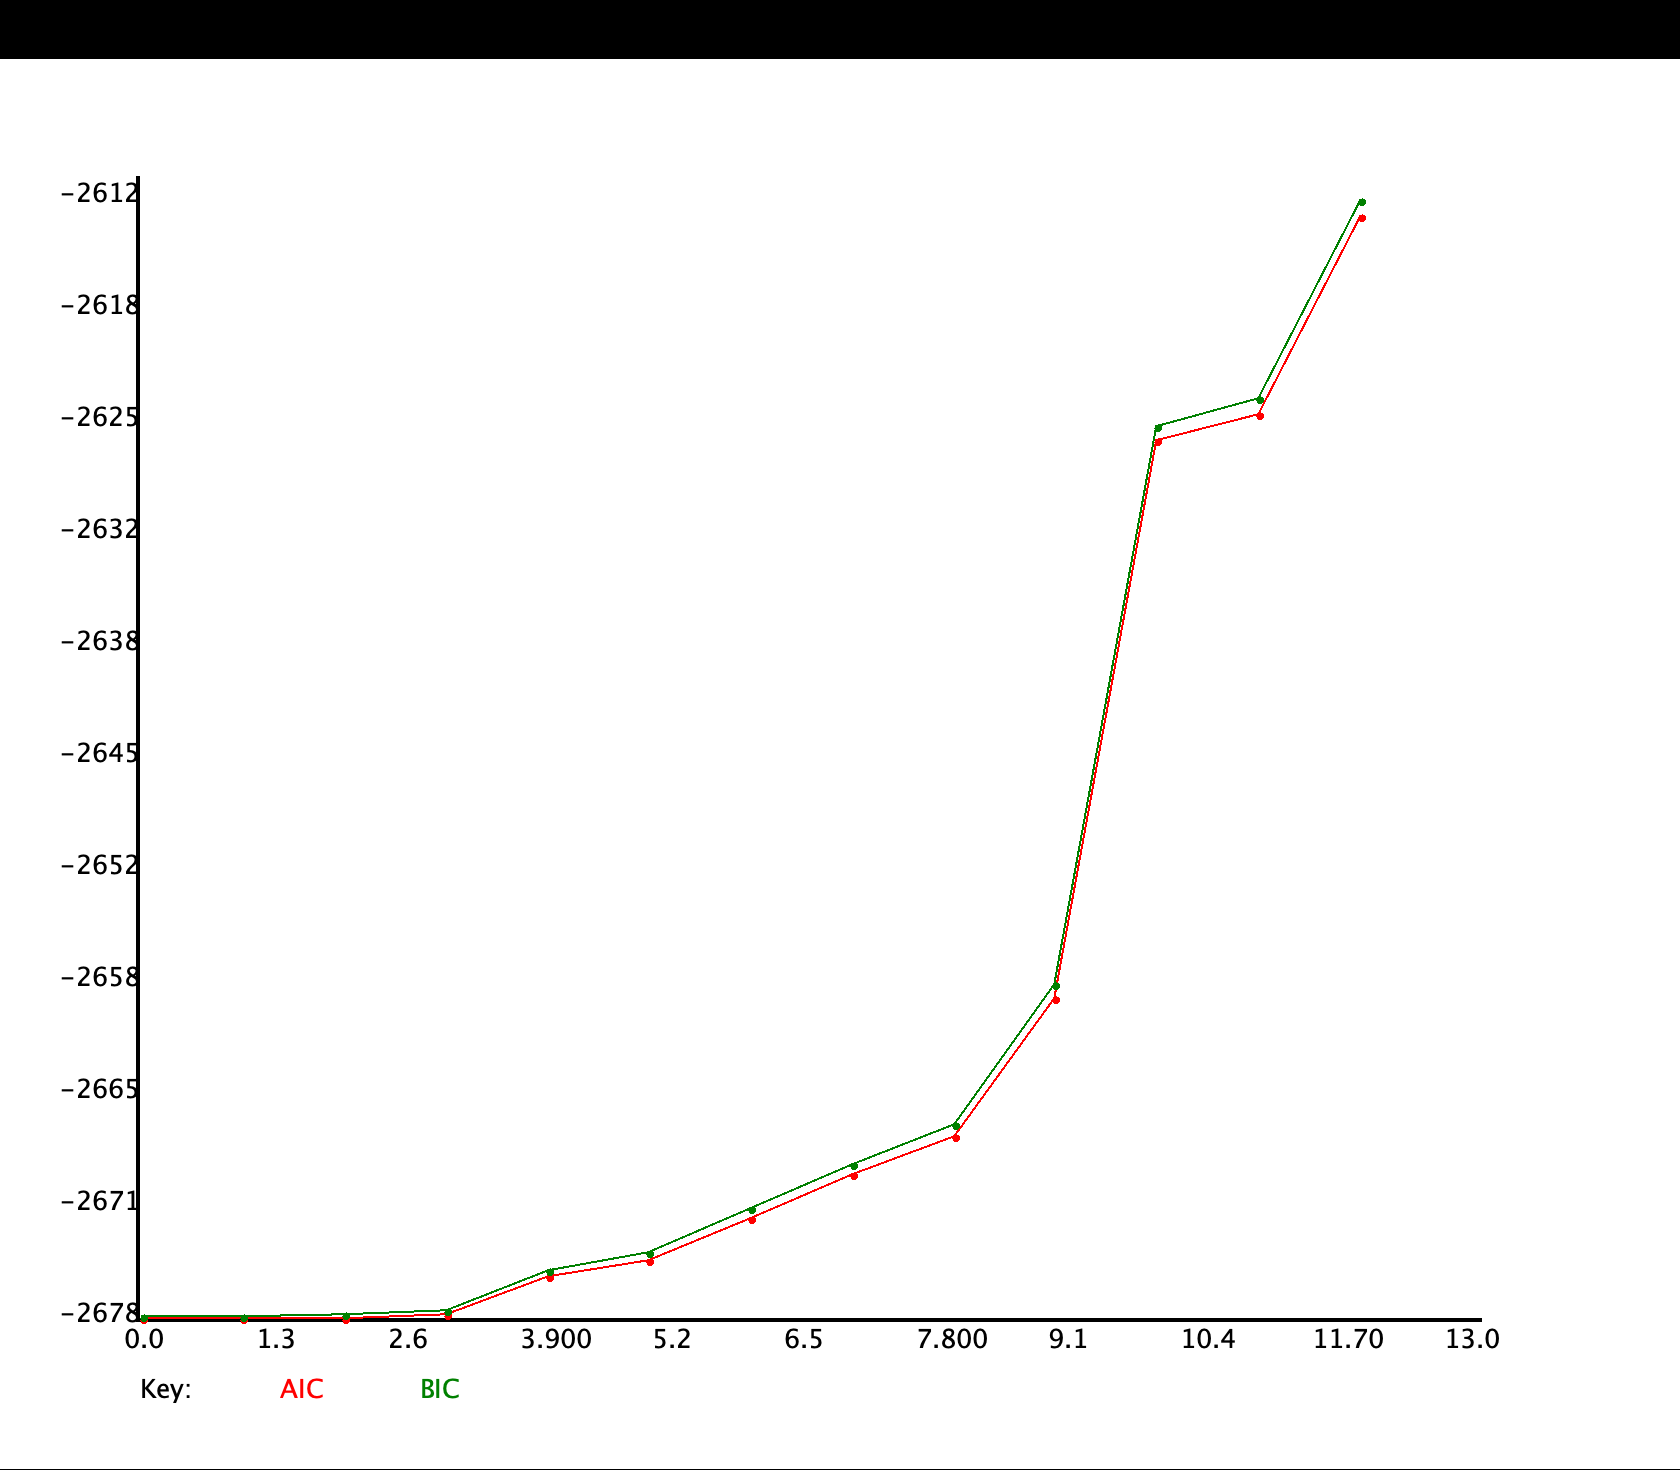
\includegraphics[width=\textwidth]{../House_Prices_Scalation_Plots/Scalation_Log1p_AIC_BIC_Forward.png}
     \end{subfigure}

     \vspace{10pt} % Add some vertical spacing between rows

     % Second Row
     \begin{subfigure}[b]{0.49\textwidth}
         \centering
         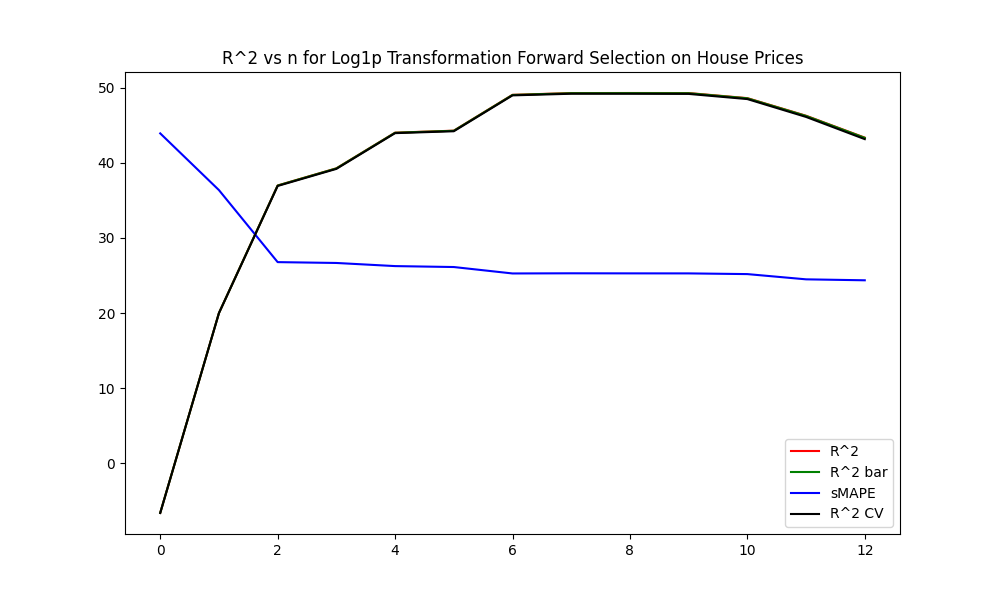
\includegraphics[width=\textwidth]{../House_Prices_Statsmodels_Plots/Statsmodels_Log1p_rSq_Forward.png}
     \end{subfigure}
     \hfill
     \begin{subfigure}[b]{0.49\textwidth}
         \centering
         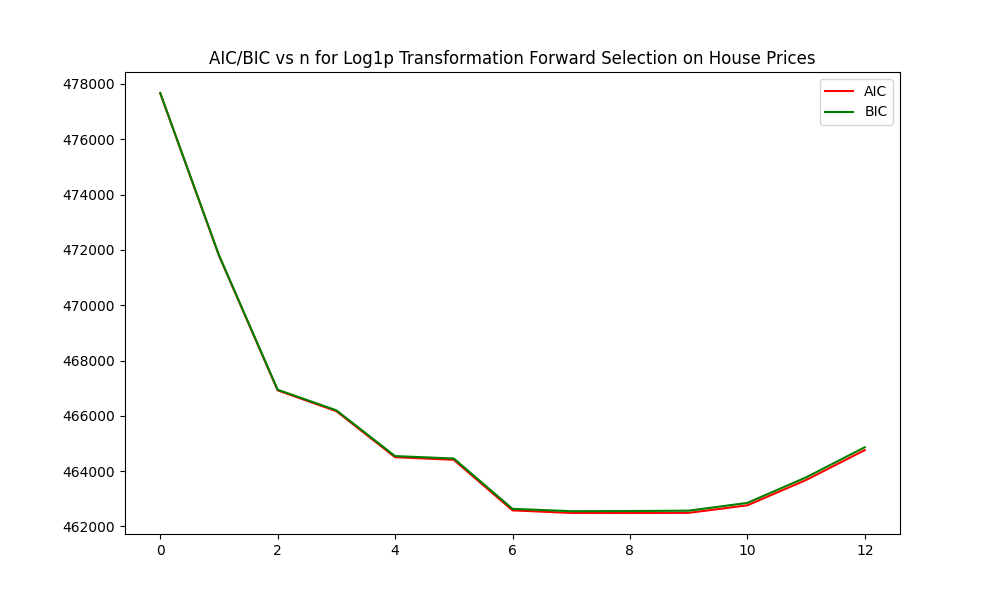
\includegraphics[width=\textwidth]{../House_Prices_Statsmodels_Plots/Statsmodels_Log1p_AIC_BIC_Forward.png}
     \end{subfigure}
     
     \caption{California House Prices Log1p Transformation Forward Selection Quality of Fit Metrics\\ Top Left: Scalation $R^2$, Top Right: Scalation AIC/BIC\\ Bottom Left: Statsmodels $R^2$, Bottom Right: Statsmodels AIC/BIC}
     \label{fig:California House Prices Log1p Transformation Forward Selection Quality of Fit Metrics}
\end{figure}

Scalation Backward Elimination Reversed: intercept, ocean proximity ISLAND, longitude, ocean proximity NEAR OCEAN, total bedrooms, households, housing median age, ocean proximity NEAR BAY, population, latitude, ocean proximity INLAND, total rooms, median income

Statsmodels Backward Elimination Reversed: intercept, latitude, longitude, median income, total rooms, population, ocean proximity INLAND, ocean proximity NEAR OCEAN, ocean proximity ISLAND, ocean proximity NEAR BAY, housing median age, households, total bedrooms

\begin{figure}[H]
     \centering
     \captionsetup{justification=centering}
     % First Row
     \begin{subfigure}[b]{0.4\textwidth}
         \centering
         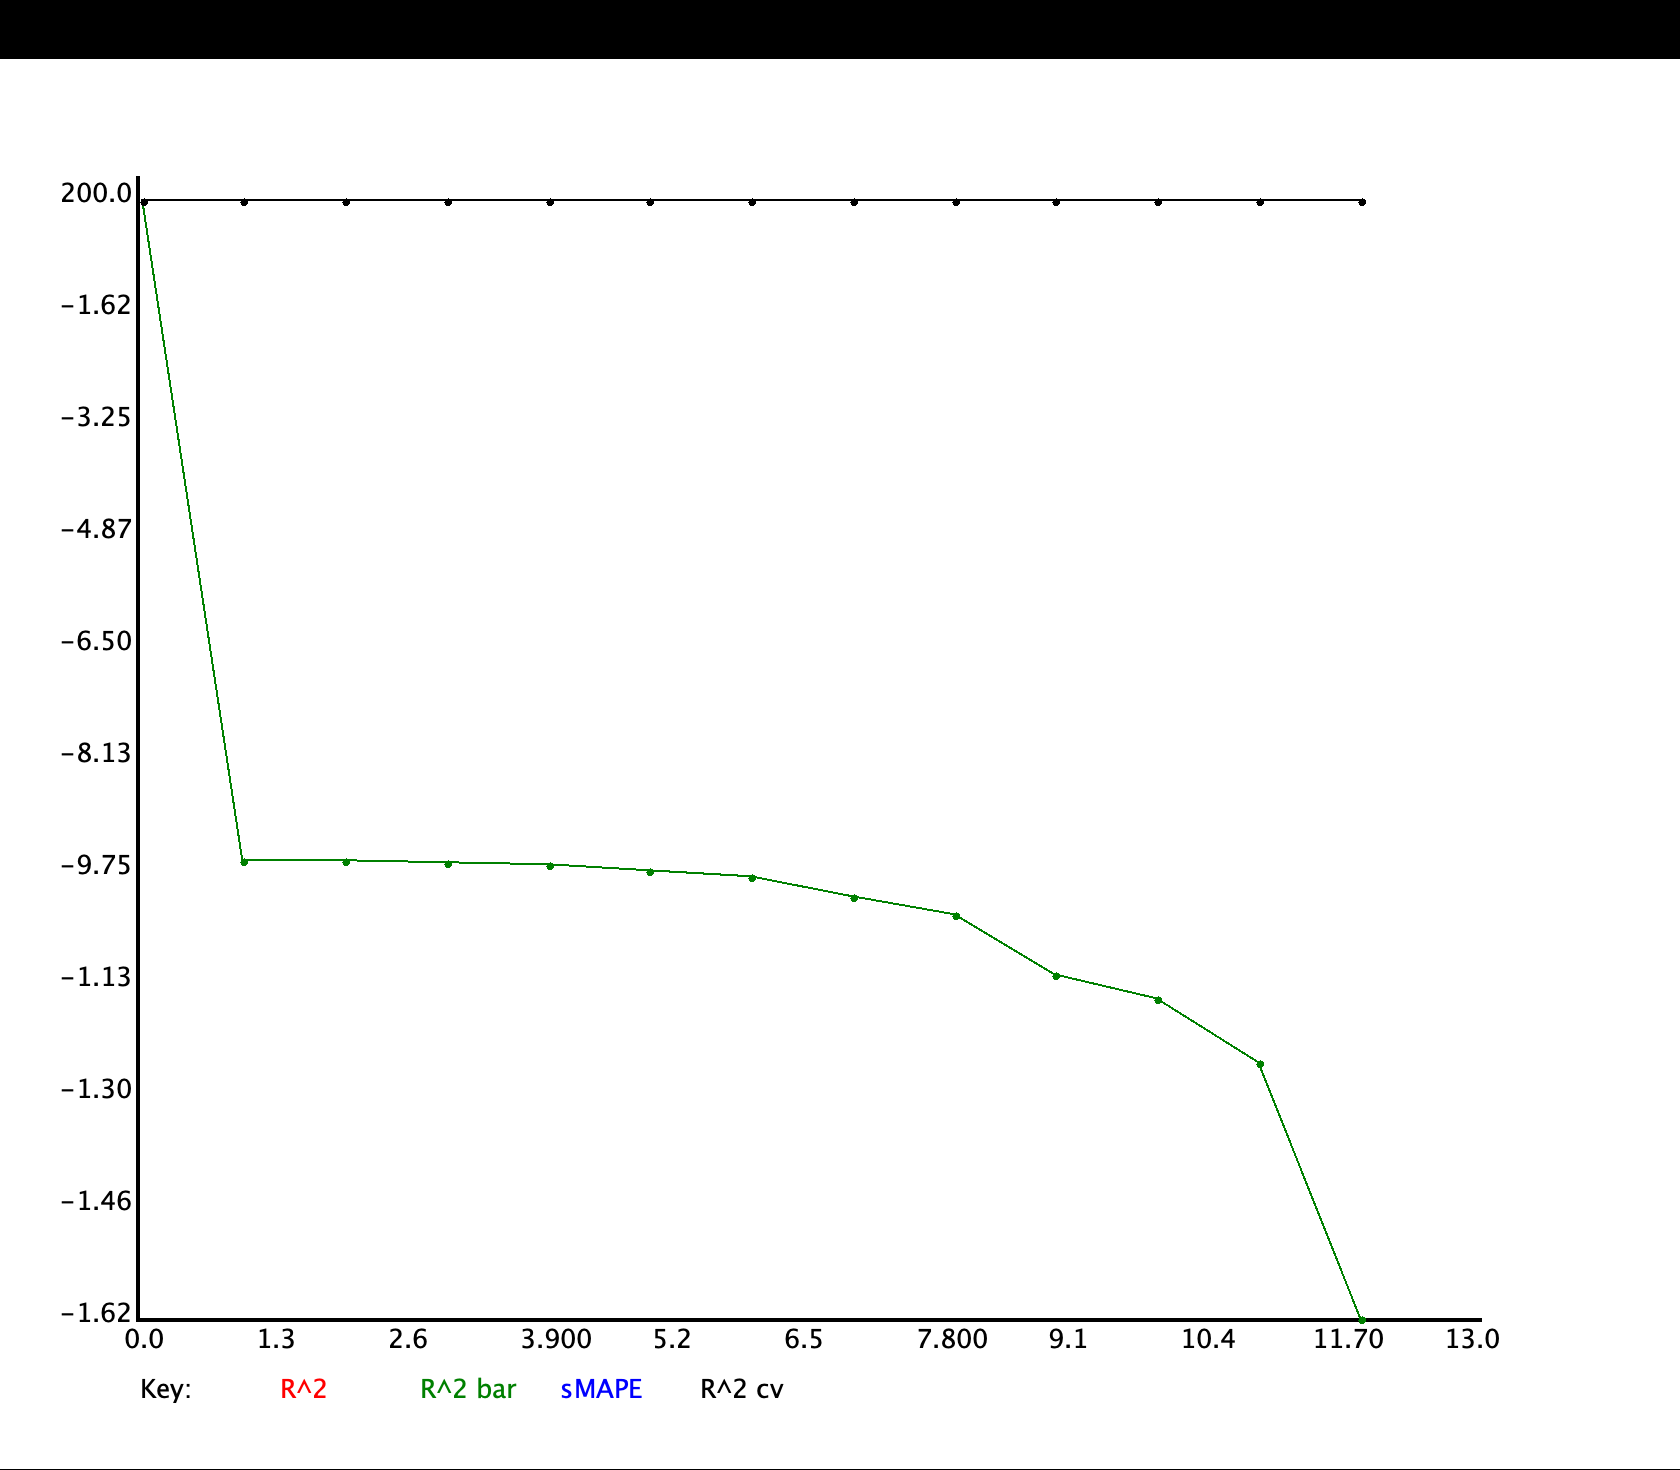
\includegraphics[width=\textwidth]{../House_Prices_Scalation_Plots/Scalation_Log1p_rSq_Backward.png}
     \end{subfigure}
     \hfill
     \begin{subfigure}[b]{0.4\textwidth}
         \centering
         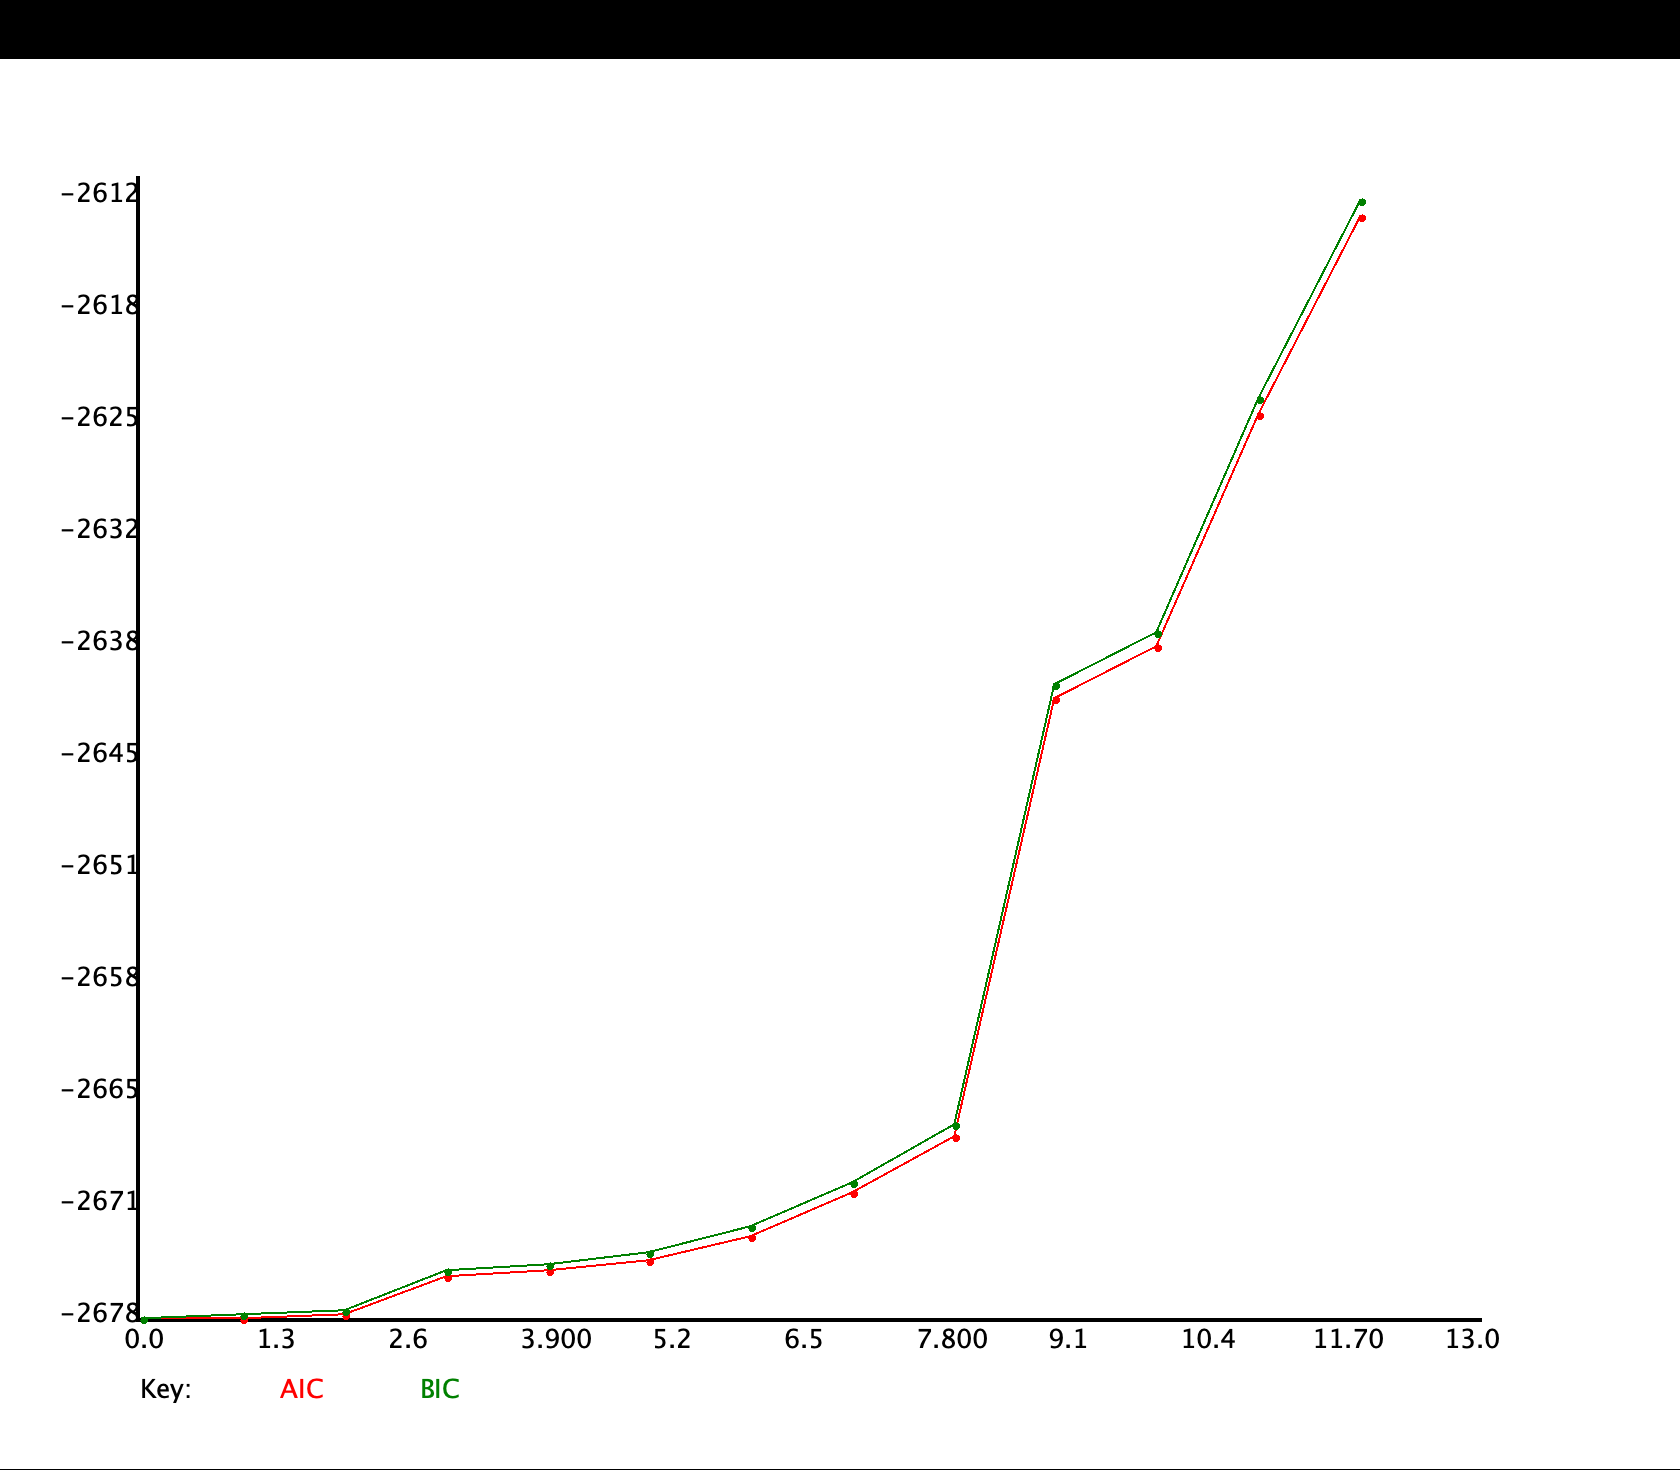
\includegraphics[width=\textwidth]{../House_Prices_Scalation_Plots/Scalation_Log1p_AIC_BIC_Backward.png}
     \end{subfigure}

     \vspace{10pt} % Add some vertical spacing between rows

     % Second Row
     \begin{subfigure}[b]{0.49\textwidth}
         \centering
         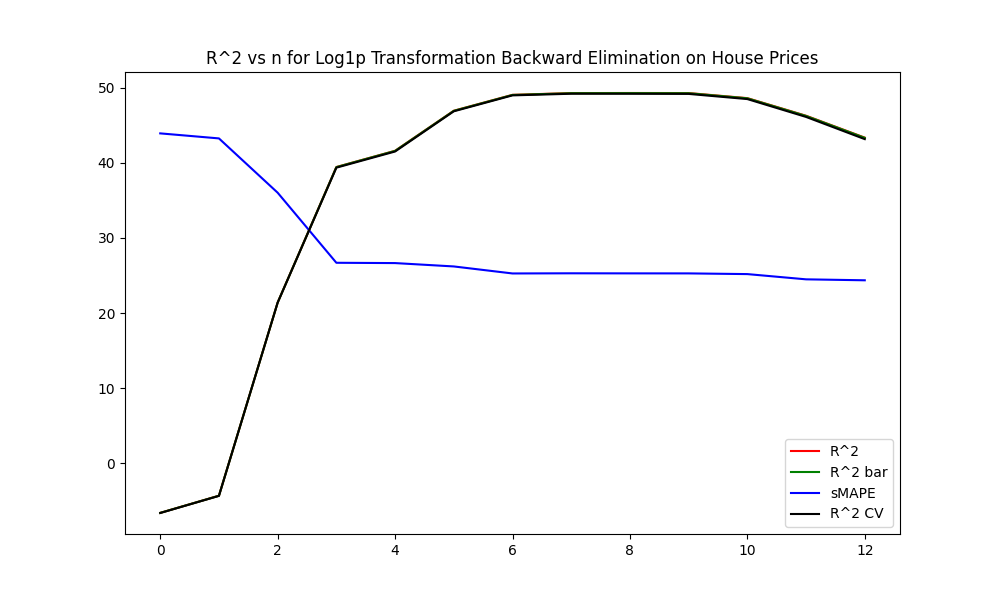
\includegraphics[width=\textwidth]{../House_Prices_Statsmodels_Plots/Statsmodels_Log1p_rSq_Backward.png}
     \end{subfigure}
     \hfill
     \begin{subfigure}[b]{0.49\textwidth}
         \centering
         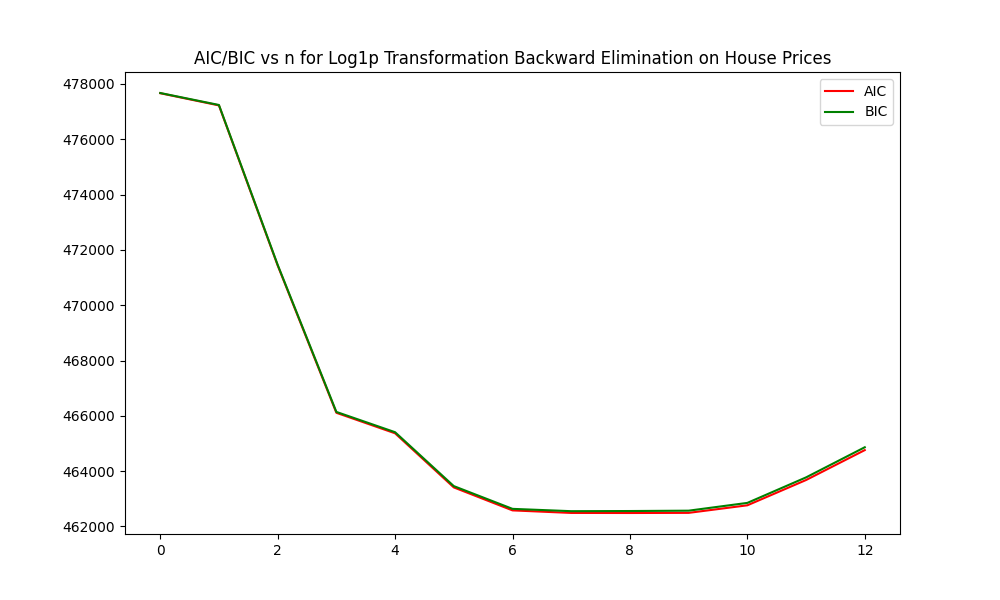
\includegraphics[width=\textwidth]{../House_Prices_Statsmodels_Plots/Statsmodels_Log1p_AIC_BIC_Backward.png}
     \end{subfigure}
     
     \caption{California House Prices Log1p Transformation Reversed Backward Elimination Quality of Fit Metrics\\ Top Left: Scalation $R^2$, Top Right: Scalation AIC/BIC\\ Bottom Left: Statsmodels $R^2$, Bottom Right: Statsmodels AIC/BIC}
     \label{fig:California House Prices Log1p Transformation Reversed Backward Elimination Quality of Fit Metrics}
\end{figure}

Scalation Stepwise Selection: intercept

Statsmodels Stepwise Selection: intercept, ocean proximity INLAND, median income, total rooms, population, longitude, latitude, ocean proximity NEAR OCEAN, ocean proximity ISLAND

\begin{figure}[H]
     \centering
     \captionsetup{justification=centering}
%     % First Row
%     \begin{subfigure}[b]{0.4\textwidth}
%         \centering
%         %\includegraphics[width=\textwidth]{../House_Prices_Scalation_Plots/Scalation_Log1p_rSq_Stepwise.png}
%     \end{subfigure}
%     \hfill
%     \begin{subfigure}[b]{0.4\textwidth}
%         \centering
%         %\includegraphics[width=\textwidth]{../House_Prices_Scalation_Plots/Scalation_Log1p_AIC_BIC_Stepwise.png}
%     \end{subfigure}
%
%     \vspace{10pt} % Add some vertical spacing between rows

     % Second Row
     \begin{subfigure}[b]{0.49\textwidth}
         \centering
         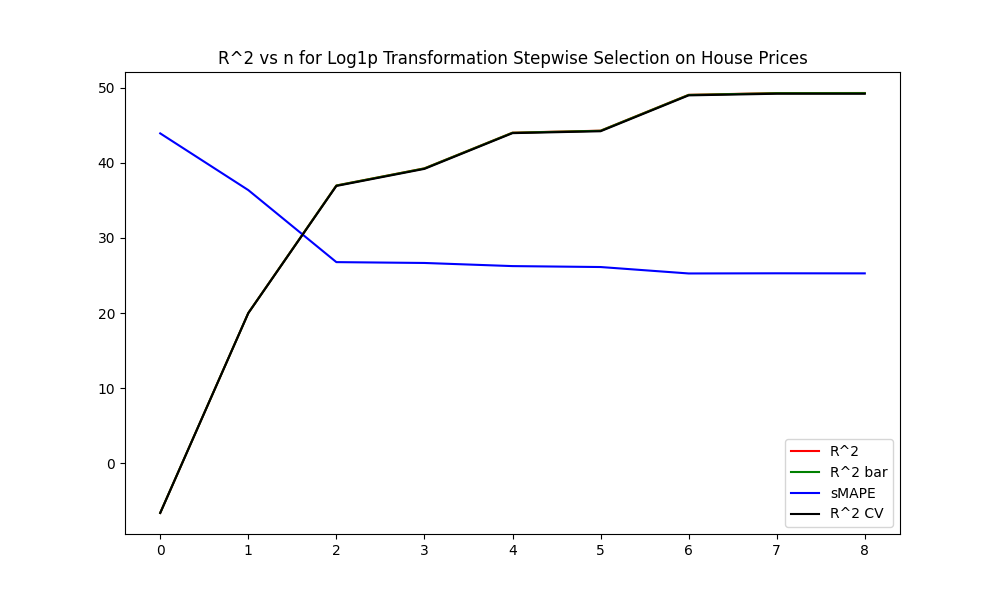
\includegraphics[width=\textwidth]{../House_Prices_Statsmodels_Plots/Statsmodels_Log1p_rSq_Stepwise.png}
     \end{subfigure}
     \hfill
     \begin{subfigure}[b]{0.49\textwidth}
         \centering
         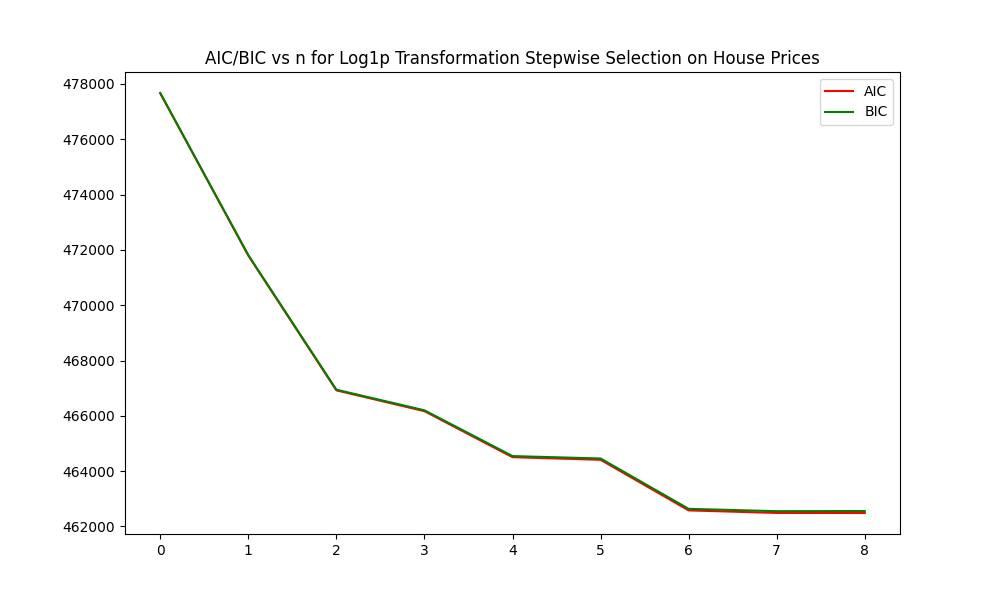
\includegraphics[width=\textwidth]{../House_Prices_Statsmodels_Plots/Statsmodels_Log1p_AIC_BIC_Stepwise.png}
     \end{subfigure}
     
     \caption{California House Prices Log1p Transformation Stepwise Selection Quality of Fit Metrics\\ Left: Statsmodels $R^2$, Right: Statsmodels AIC/BIC}
     \label{fig:California House Prices Log1p Transformation Stepwise Selection Quality of Fit Metrics}
\end{figure}

\subsection{Box-Cox Transformation}

\subsubsection{Quality of Fit}

Scalation California House Prices Box-Cox Lambda Used: $1$

\noindent Statsmodels California House Prices Box-Cox lambda Used: $1$

\begin{table}[H]
\centering
\caption{Scalation - California House Prices Box-Cox Transformation}
\label{tab:Scalation - House Prices Box-Cox Transformation}
\begin{tabular}{|c|c|c|} \hline 
Metric & In-Sample & 80-20 Split \\ \hline \hline 
rSq &0.646464 & 0.643048 \\ \hline 
rSqBar &0.646256 &      0.642838 \\ \hline 
sst &2.72264e+14 &      5.31945e+13 \\ \hline 
sse &9.62553e+13 &      1.89879e+13 \\ \hline 
sde &68636.8 &  68138.4 \\ \hline 
mse0 &4.71078e+09 &     4.64706e+09 \\ \hline 
rmse &68635.1 & 68169.4 \\ \hline 
mae &49748.2 &  49532.1 \\ \hline 
smape &26.2930 &        26.4602 \\ \hline 
m &20433.0 &    4086.00 \\ \hline 
dfr &12.0000 &  12.0000 \\ \hline 
df &20420.0 &   20420.0 \\ \hline 
fStat &3111.61 &        3065.54 \\ \hline 
aic &-256520 &  -51247.9 \\ \hline 
bic &-256417 &  -51165.8 \\ \hline 
\end{tabular}
\end{table}

\begin{table}[H]
\centering
\caption{Statsmodels - California House Prices Box-Cox Transformation}
\label{tab:Statsmodels - House Prices Box-Cox Transformation}
\begin{tabular}{|c|c|c|}\hline
Metric & In-Sample & 80-20 Split \\ \hline \hline
rSq & 0.6465 & 0.6534 \\ \hline
rSqBar & 0.6463 & 0.6523 \\ \hline
sst & 272264434648930.0000 & 54723646809444.8438 \\ \hline
sse & 96255324900327.4375 & 18969618571471.6602 \\ \hline
sde & 68656.9511 & 68236.8212 \\ \hline
mse0 & 4713776929.4969 & 4641453039.2639 \\ \hline
rmse & 68656.9511 & 68128.2103 \\ \hline
mae & 49581.1591 & 49928.6702 \\ \hline
smape & 25.9523 & 25.9125 \\ \hline
m & 20433.0000 & 4087.0000 \\ \hline
dfr & 12.0000 & 13.0000 \\ \hline
df & 20420.0000 & 4074.0000 \\ \hline
fStat & 3111.6080 & 590.6688 \\ \hline
aic & 513118.9804 & 90995.6448 \\ \hline
bic & 513222.0042 & 91077.7471 \\ \hline
\end{tabular}
\end{table}

\begin{table}[H]
\centering
\caption{Scalation - California House Prices Box-Cox Transformation CV}
\label{tab:Scalation - House Prices Box-Cox Transformation CV}
\begin{tabular}{|c|c|c|c|c|c|}\hline
Metric & num folds & min & max & mean & stdev \\ \hline \hline
rSq & 5 & 0.628 & 0.661 & 0.645 & 0.012 \\ \hline
rSqBar & 5 & 0.628 & 0.661 & 0.645 & 0.012 \\ \hline
sst & 5 & 53194492241132.980 & 57310203956796.625 & 54411355017051.000 & 1675890609056.710 \\ \hline
sse & 5 & 18091271374124.582 & 21300107623724.016 & 19326273860287.406 & 1203800943359.010 \\ \hline
sde & 5 & 66545.500 & 72143.458 & 68734.562 & 2094.101 \\ \hline
mse0 & 5 & 4427623929.056 & 5212948512.904 & 4729876128.313 & 294615992.012 \\ \hline
rmse & 5 & 66540.393 & 72200.751 & 68748.019 & 2117.175 \\ \hline
mae & 5 & 48559.672 & 51928.415 & 49805.806 & 1284.904 \\ \hline
smape & 5 & 25.797 & 26.836 & 26.328 & 0.382 \\ \hline
m & 5 & 4086.000 & 4086.000 & 4086.000 & 0.000 \\ \hline
dfr & 5 & 12.000 & 12.000 & 12.000 & 0.000 \\ \hline
df & 5 & 20420.000 & 20420.000 & 20420.000 & 0.000 \\ \hline
fStat & 5 & 2876.848 & 3321.528 & 3096.873 & 162.980 \\ \hline
aic & 5 & -51497.014 & -51151.361 & -51284.395 & 129.672 \\ \hline
bic & 5 & -51414.915 & -51069.262 & -51202.295 & 129.672 \\ \hline
\end{tabular}
\end{table}

\begin{table}[H]
\centering
\caption{Statsmodels - California House Prices Box-Cox Transformation CV}
\label{tab:Statsmodels - House Prices Box-Cox Transformation CV}
\begin{tabular}{|c|c|c|c|c|c|}\hline
Metric & num folds & min & max & mean & stdev \\ \hline \hline
rSq & 5 & 0.6371 & 0.6625 & 0.6512 & 0.0081 \\ \hline
rSqBar & 5 & 0.6360 & 0.6615 & 0.6502 & 0.0082 \\ \hline
sst & 5 & 53541750406767.3438 & 54912923487891.5781 & 54447676367709.7031 & 499826929365.4288 \\ \hline
sse & 5 & 18534929031539.1953 & 19430253836534.6719 & 18986690905997.2578 & 290286886054.2943 \\ \hline
sde & 5 & 67450.4655 & 69068.8193 & 68268.8923 & 524.0756 \\ \hline
mse0 & 5 & 4535093964.1642 & 4755323993.2782 & 4646089322.7525 & 71316203.1957 \\ \hline
rmse & 5 & 67343.1063 & 68958.8573 & 68160.2197 & 523.2348 \\ \hline
mae & 5 & 48691.5295 & 50112.9423 & 49618.6076 & 495.5004 \\ \hline
smape & 5 & 25.6318 & 26.3366 & 25.9756 & 0.2627 \\ \hline
m & 5 & 4086.0000 & 4087.0000 & 4086.6000 & 0.4899 \\ \hline
dfr & 5 & 13.0000 & 13.0000 & 13.0000 & 0.0000 \\ \hline
df & 5 & 4073.0000 & 4074.0000 & 4073.6000 & 0.4899 \\ \hline
fStat & 5 & 550.0388 & 615.0713 & 585.5530 & 20.7836 \\ \hline
aic & 5 & 90900.9013 & 91072.4203 & 90990.3359 & 58.0078 \\ \hline
bic & 5 & 90983.0036 & 91154.5195 & 91072.4370 & 58.0072 \\ \hline
\end{tabular}
\end{table}

\begin{figure}[H]
     \centering
     \captionsetup{justification=centering}
     % First Row
     \begin{subfigure}[b]{0.4\textwidth}
         \centering
         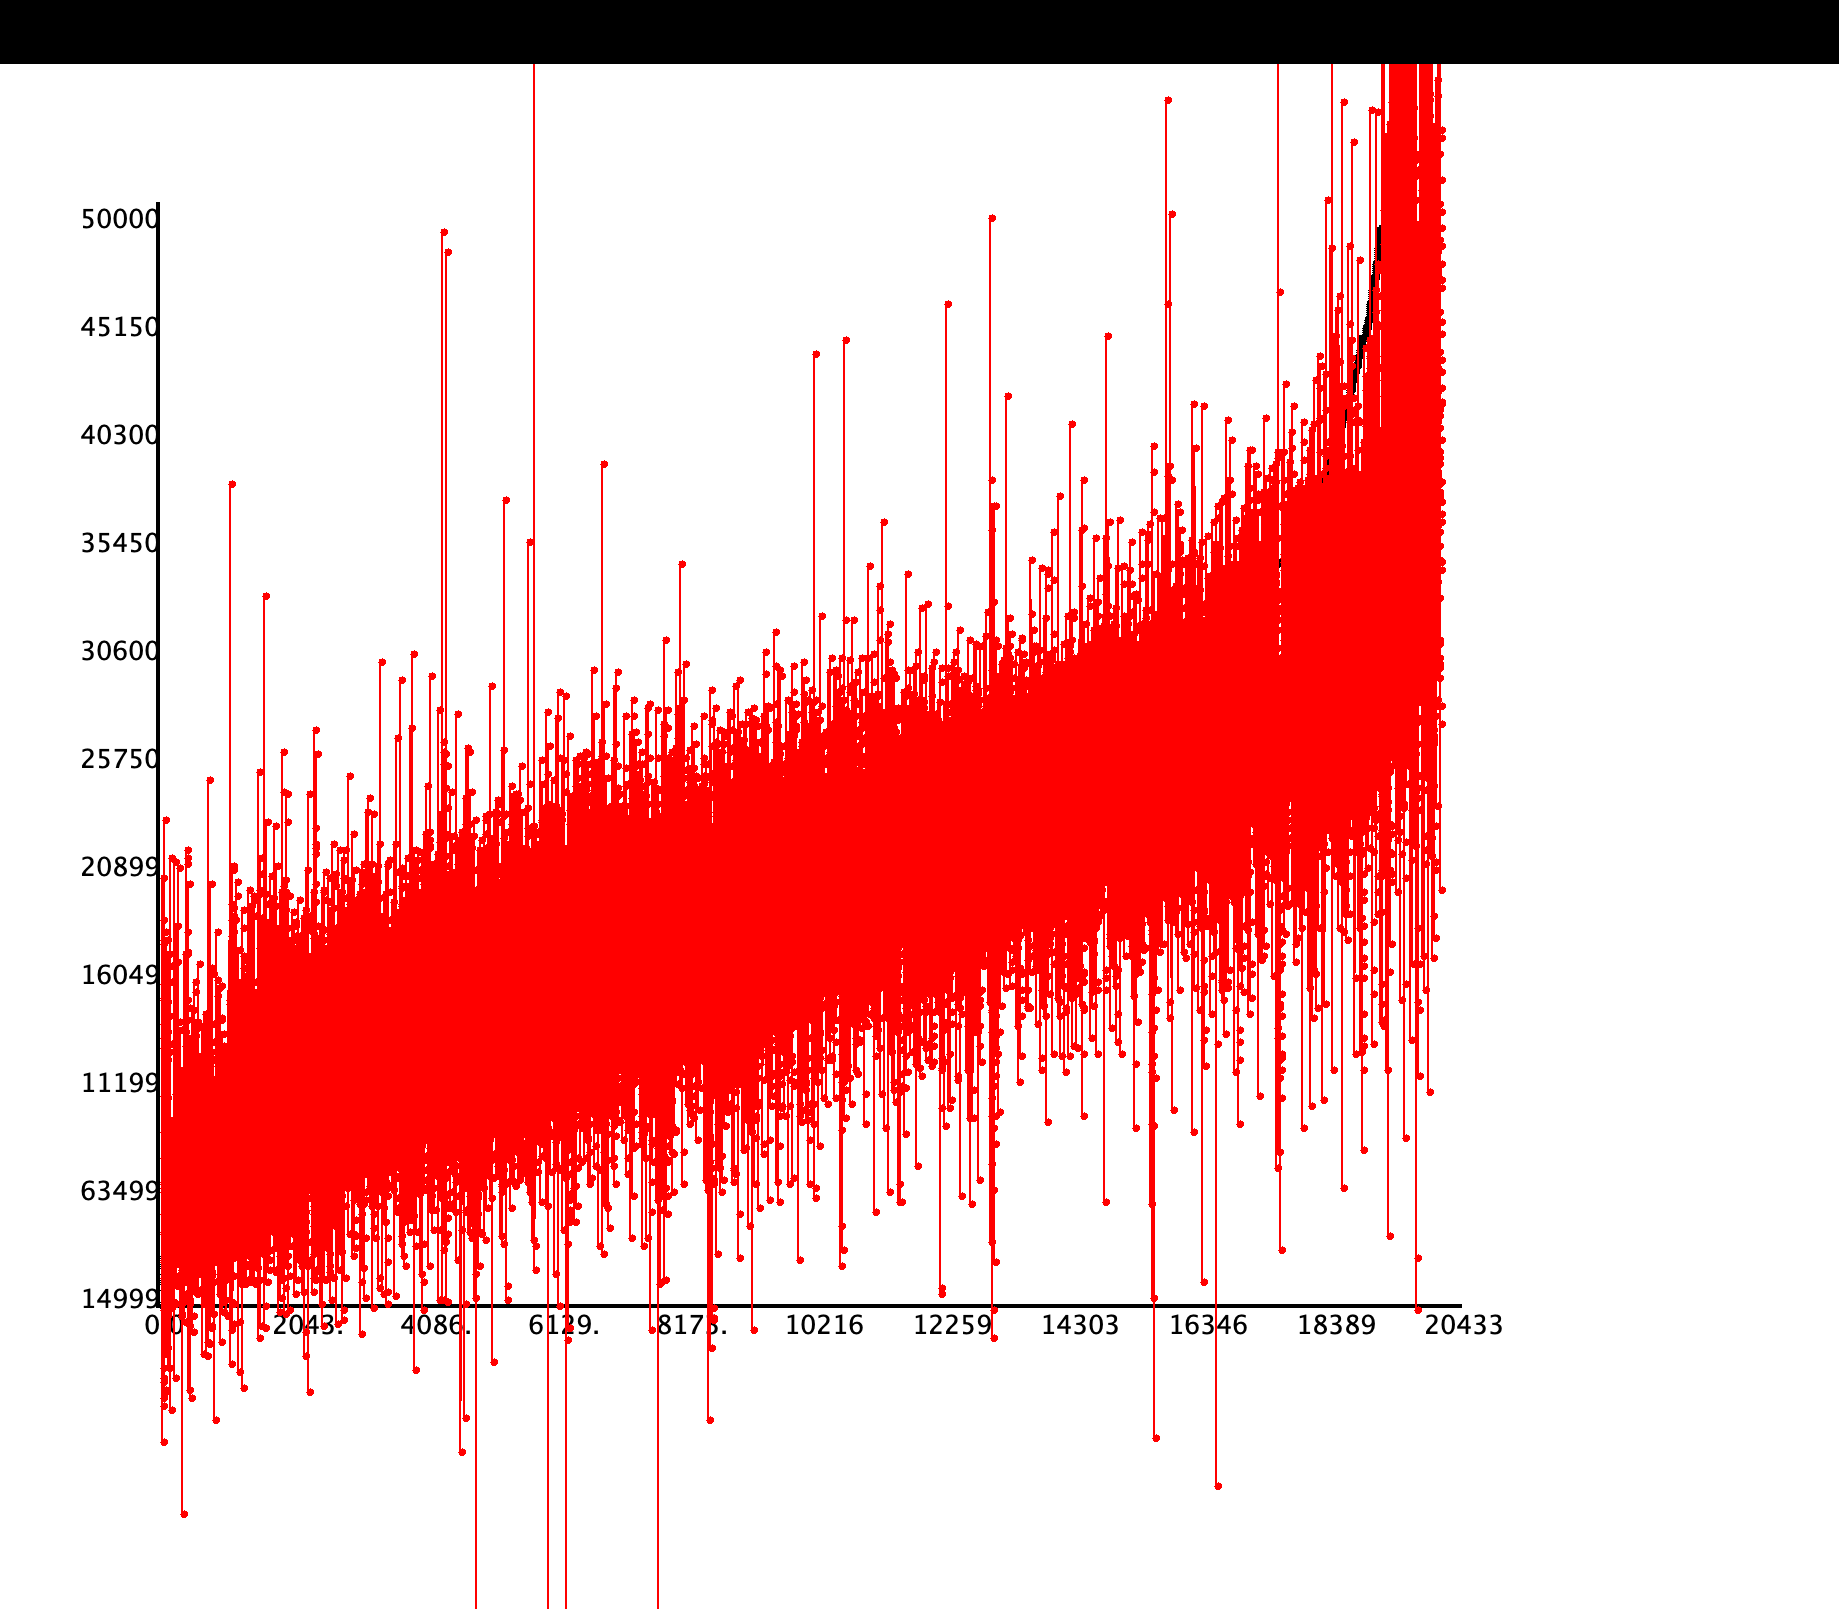
\includegraphics[width=\textwidth]{../House_Prices_Scalation_Plots/Scalation_BoxCox_In_Sample.png}
     \end{subfigure}
     \hfill
     \begin{subfigure}[b]{0.4\textwidth}
         \centering
         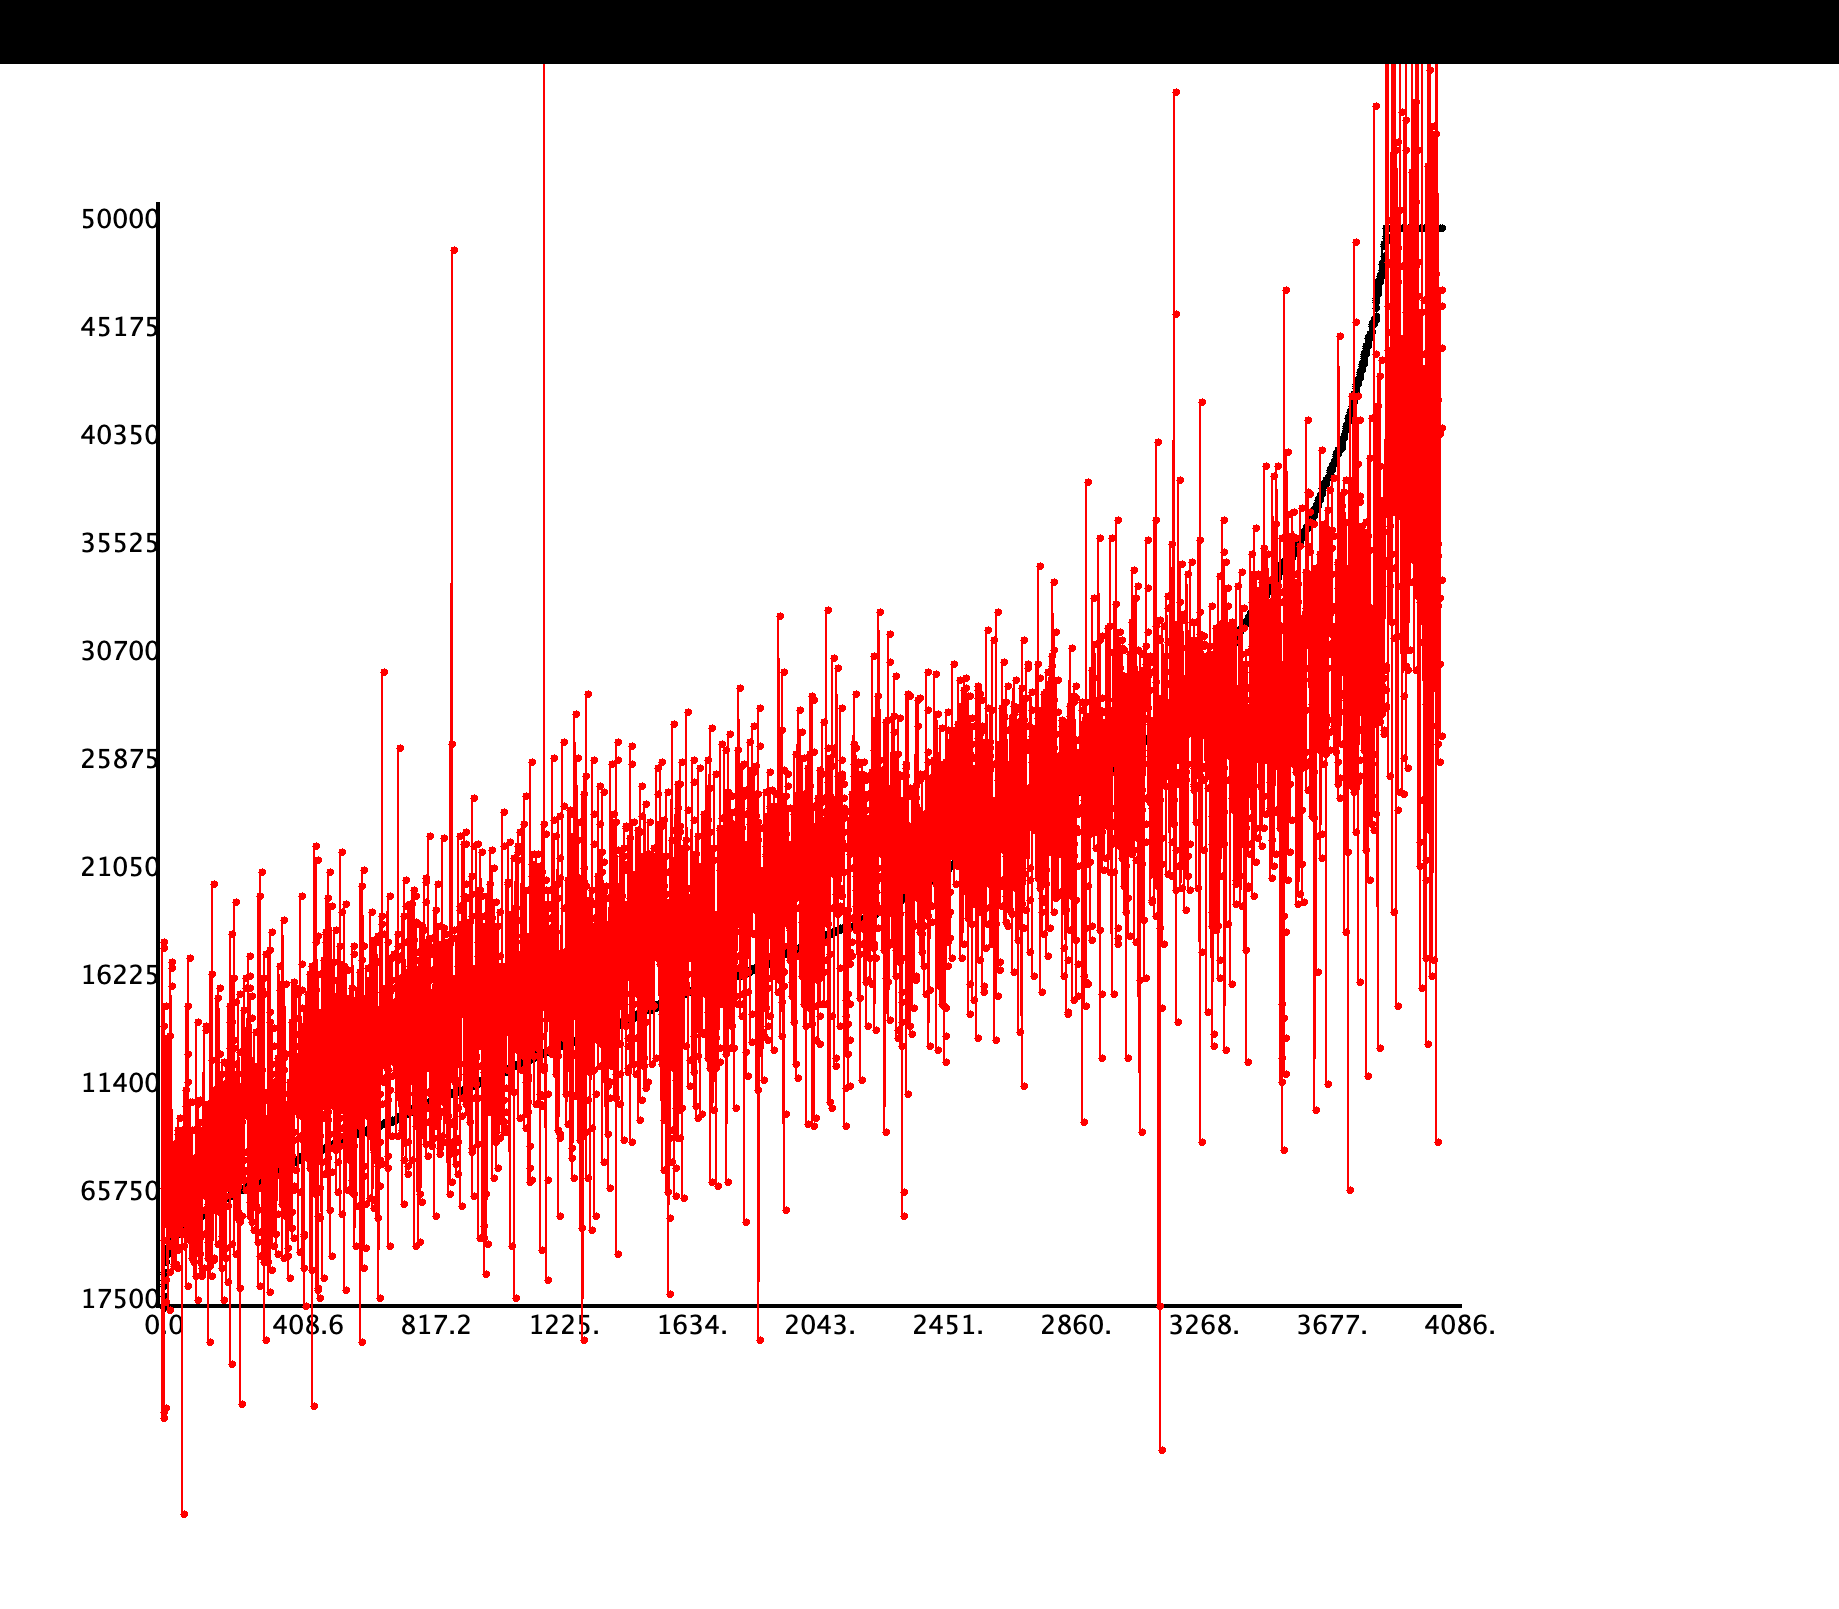
\includegraphics[width=\textwidth]{../House_Prices_Scalation_Plots/Scalation_BoxCox_80_20.png}
     \end{subfigure}

     \vspace{10pt} % Add some vertical spacing between rows

     % Second Row
     \begin{subfigure}[b]{0.49\textwidth}
         \centering
         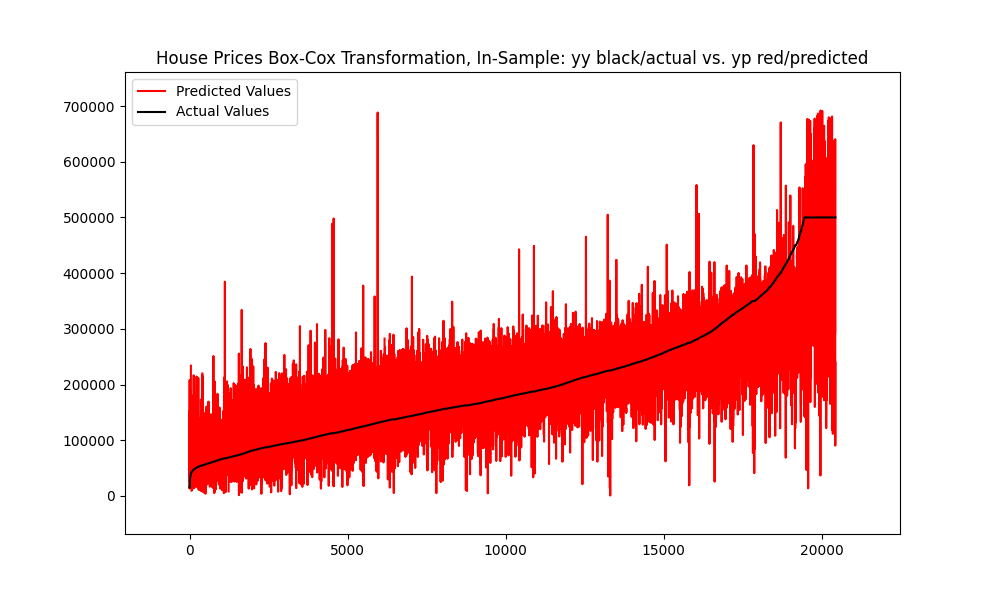
\includegraphics[width=\textwidth]{../House_Prices_Statsmodels_Plots/Statsmodels_BoxCox_In_Sample.png}
     \end{subfigure}
     \hfill
     \begin{subfigure}[b]{0.49\textwidth}
         \centering
         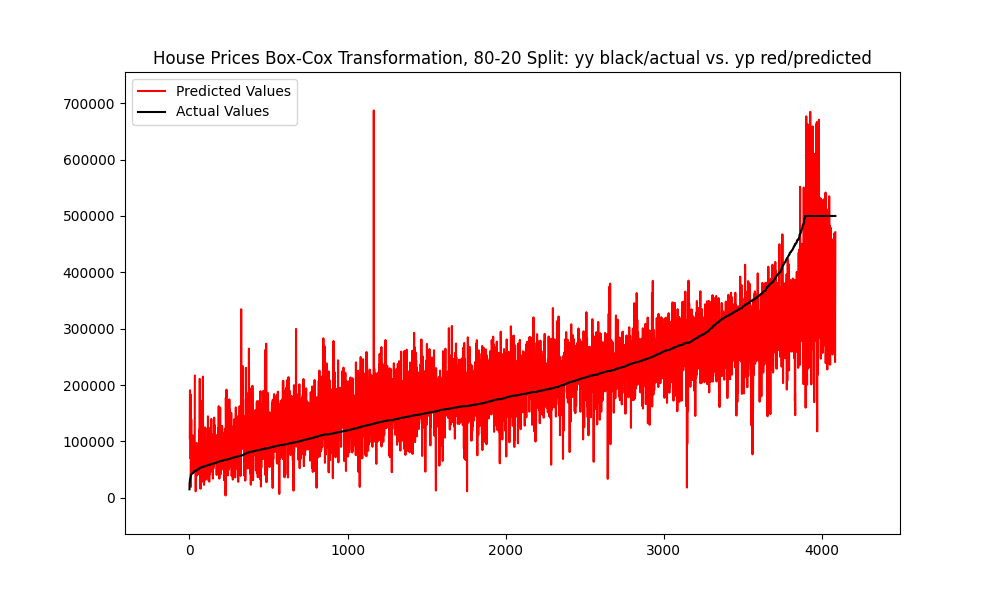
\includegraphics[width=\textwidth]{../House_Prices_Statsmodels_Plots/Statsmodels_BoxCox_80_20.png}
     \end{subfigure}
     
     \caption{California House Prices Box-Cox Transformation Plots\\ Top Left: Scalation In-Sample, Top Right: Scalation Out-of-Sample\\ Bottom Left: Statsmodels In-Sample, Bottom Right: Statsmodels Out-of-Sample\\ black: actual y-values, red: predicted y-values}
     \label{fig:California House Prices Box-Cox Transformation Plots}
\end{figure}

\subsubsection{Feature Selection}

Scalation Forward Selection: intercept, median income, ocean proximity INLAND, housing median age, total bedrooms, population, total rooms, households, ocean proximity ISLAND, latitude, longitude, ocean proximity NEAR BAY, ocean proximity NEAR OCEAN

Statsmodels Forward Selection: intercept, median income, ocean proximity INLAND, housing median age, total bedrooms, population, households, ocean proximity ISLAND, ocean proximity NEAR OCEAN, total rooms, longitude, latitude, ocean proximity NEAR BAY

\begin{figure}[H]
     \centering
     \captionsetup{justification=centering}
     % First Row
     \begin{subfigure}[b]{0.4\textwidth}
         \centering
         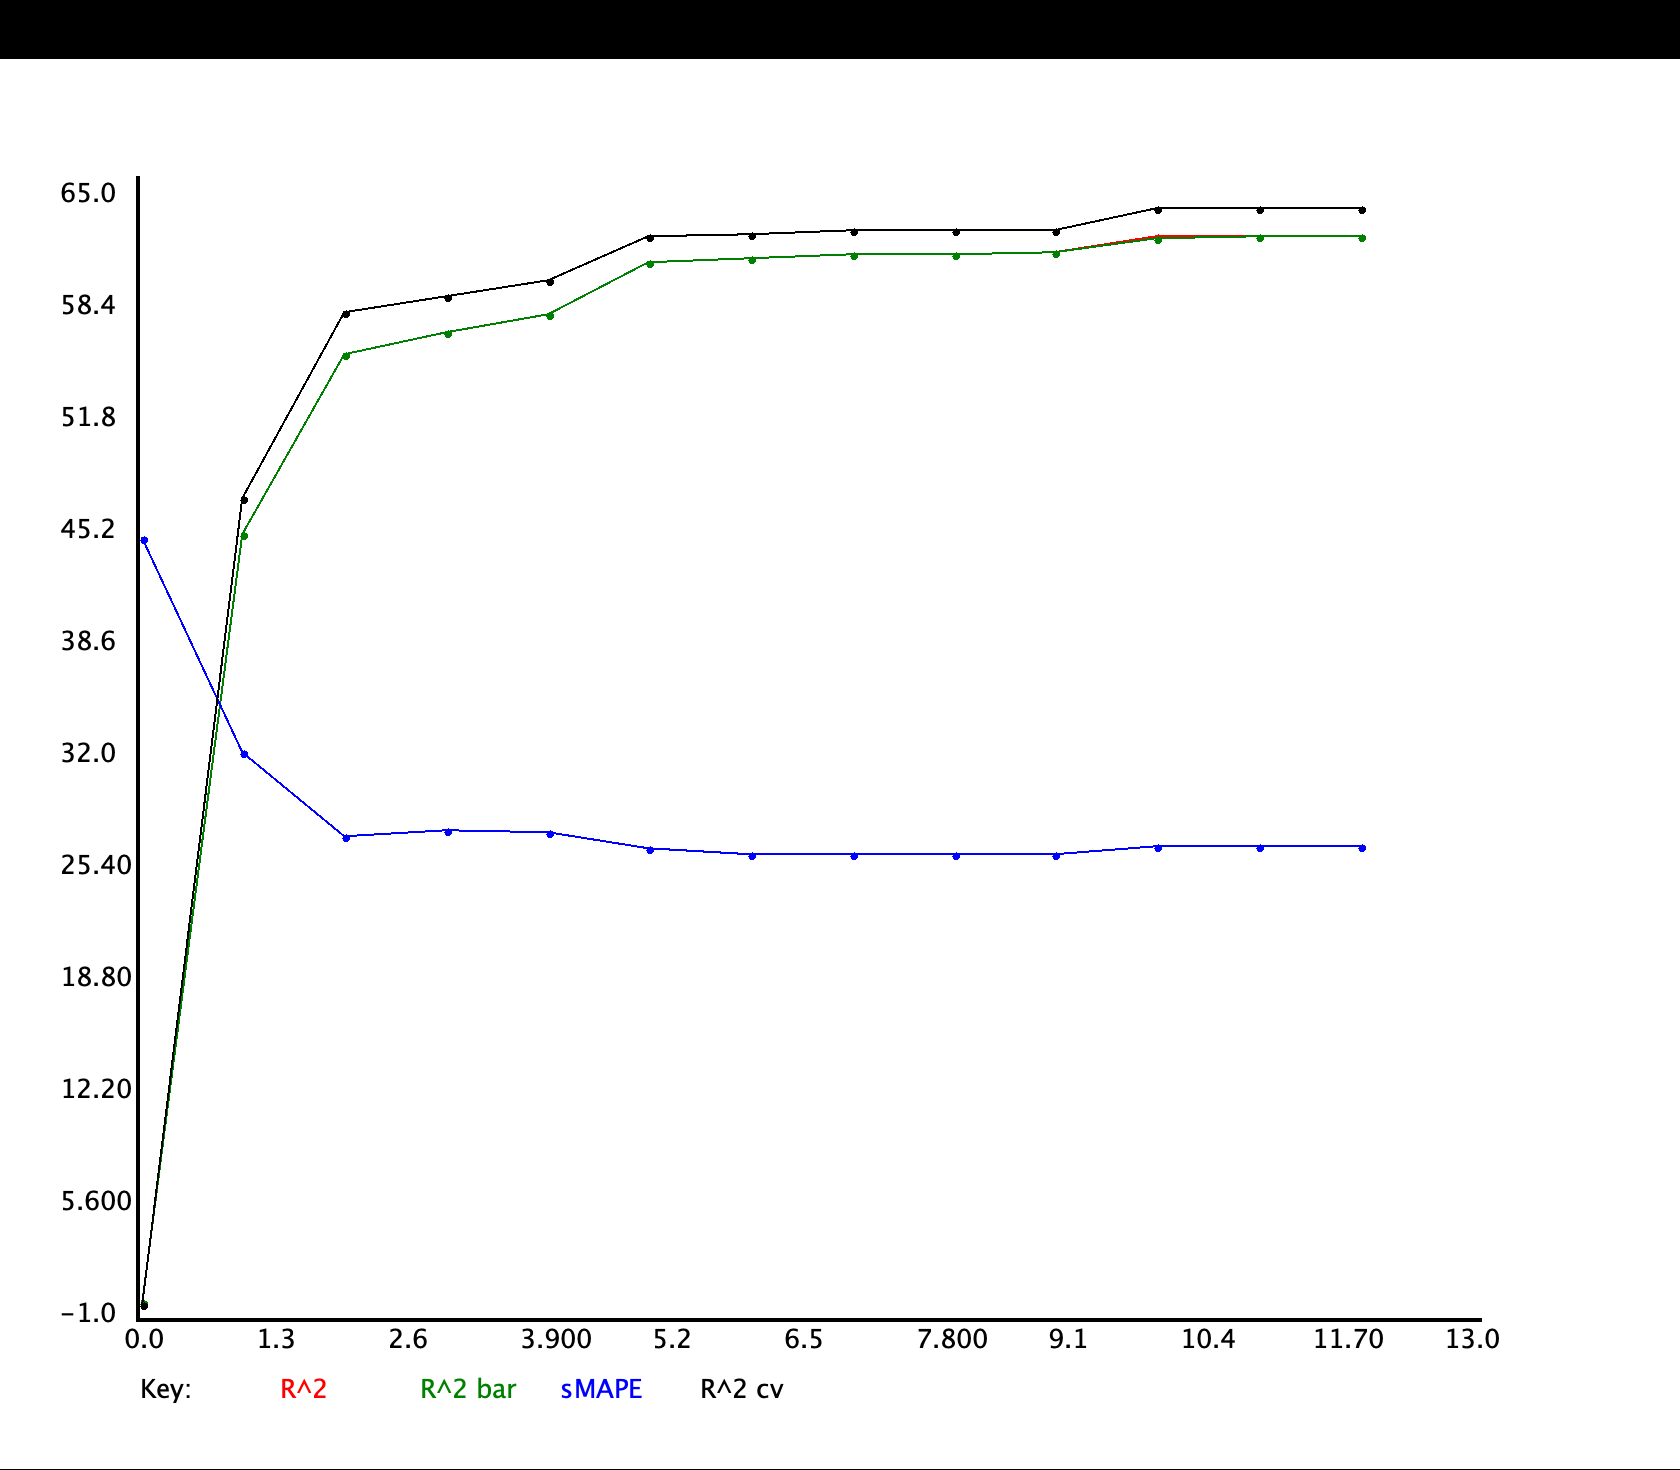
\includegraphics[width=\textwidth]{../House_Prices_Scalation_Plots/Scalation_BoxCox_rSq_Forward.png}
     \end{subfigure}
     \hfill
     \begin{subfigure}[b]{0.4\textwidth}
         \centering
         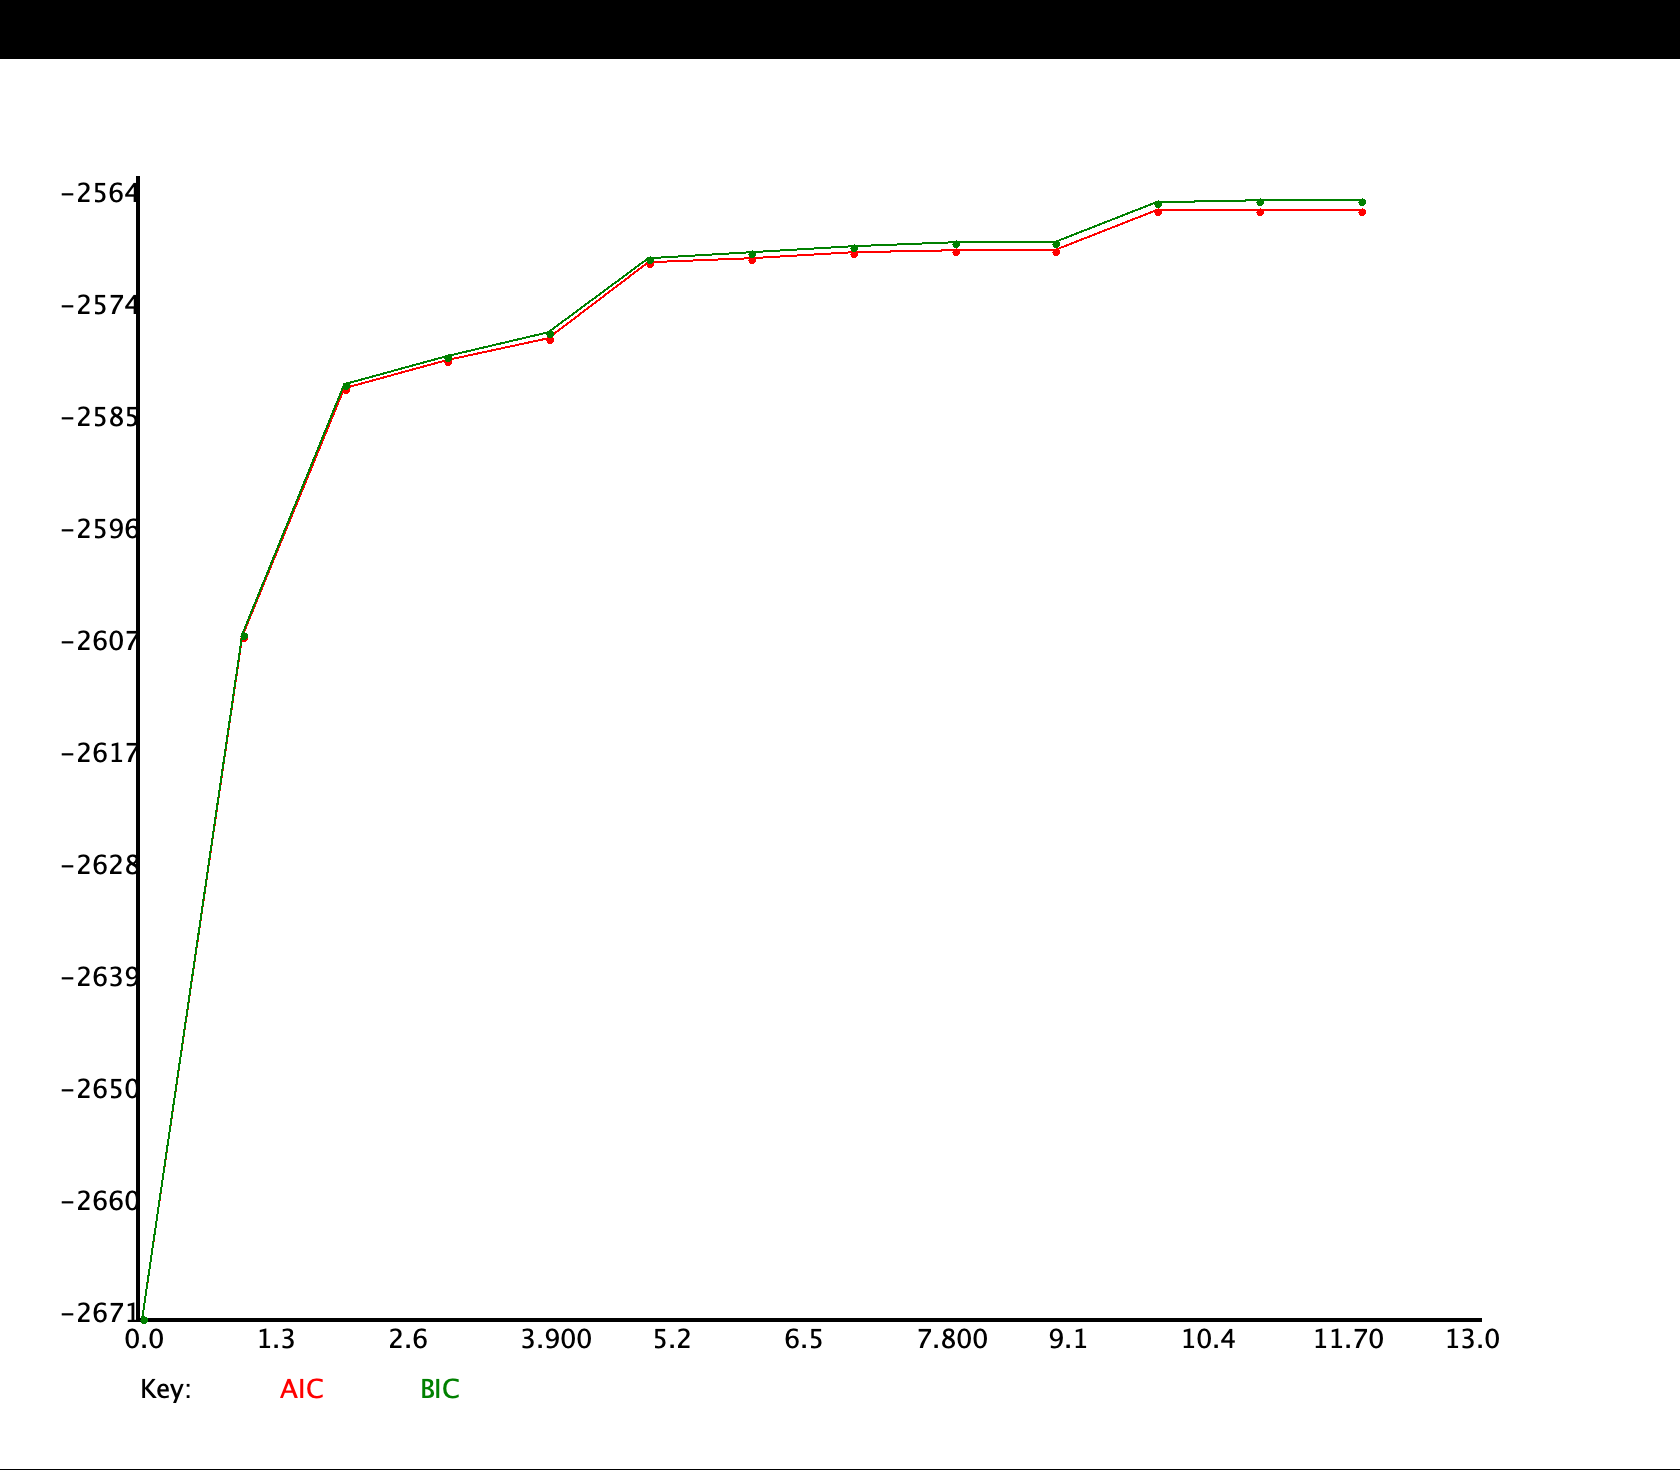
\includegraphics[width=\textwidth]{../House_Prices_Scalation_Plots/Scalation_BoxCox_AIC_BIC_Forward.png}
     \end{subfigure}

     \vspace{10pt} % Add some vertical spacing between rows

     % Second Row
     \begin{subfigure}[b]{0.49\textwidth}
         \centering
         \includegraphics[width=\textwidth]{../House_Prices_Statsmodels_Plots/Statsmodels_BoxCox_rSq_Forward.png}
     \end{subfigure}
     \hfill
     \begin{subfigure}[b]{0.49\textwidth}
         \centering
         \includegraphics[width=\textwidth]{../House_Prices_Statsmodels_Plots/Statsmodels_BoxCox_AIC_BIC_Forward.png}
     \end{subfigure}
     
     \caption{California House Prices Box-Cox Transformation Forward Selection Quality of Fit Metrics\\ Top Left: Scalation $R^2$, Top Right: Scalation AIC/BIC\\ Bottom Left: Statsmodels $R^2$, Bottom Right: Statsmodels AIC/BIC}
     \label{fig:California House Prices Box-Cox Transformation Forward Selection Quality of Fit Metrics}
\end{figure}

Scalation Backward Elimination Reversed: intercept, median income, latitude, longitude, total bedrooms, population, housing median age, ocean proximity INLAND, total rooms, households, ocean proximity ISLAND, ocean proximity NEAR BAY, ocean proximity NEAR OCEAN

Statsmodels Backward Elimination Reversed: intercept, median income, latitude, longitude, total bedrooms, population, housing median age, ocean proximity INLAND, households, total rooms, ocean proximity ISLAND, ocean proximity NEAR BAY, ocean proximity NEAR OCEAN

\begin{figure}[H]
     \centering
     \captionsetup{justification=centering}
     % First Row
     \begin{subfigure}[b]{0.4\textwidth}
         \centering
         \includegraphics[width=\textwidth]{../House_Prices_Scalation_Plots/Scalation_BoxCox_rSq_Backward.png}
     \end{subfigure}
     \hfill
     \begin{subfigure}[b]{0.4\textwidth}
         \centering
         \includegraphics[width=\textwidth]{../House_Prices_Scalation_Plots/Scalation_BoxCox_AIC_BIC_Backward.png}
     \end{subfigure}

     \vspace{10pt} % Add some vertical spacing between rows

     % Second Row
     \begin{subfigure}[b]{0.49\textwidth}
         \centering
         \includegraphics[width=\textwidth]{../House_Prices_Statsmodels_Plots/Statsmodels_BoxCox_rSq_Backward.png}
     \end{subfigure}
     \hfill
     \begin{subfigure}[b]{0.49\textwidth}
         \centering
         \includegraphics[width=\textwidth]{../House_Prices_Statsmodels_Plots/Statsmodels_BoxCox_AIC_BIC_Backward.png}
     \end{subfigure}
     
     \caption{California House Prices Box-Cox Transformation Reversed Backward Elimination Quality of Fit Metrics\\ Top Left: Scalation $R^2$, Top Right: Scalation AIC/BIC\\ Bottom Left: Statsmodels $R^2$, Bottom Right: Statsmodels AIC/BIC}
     \label{fig:California House Prices Box-Cox Transformation Reversed Backward Elimination Quality of Fit Metrics}
\end{figure}

Scalation Stepwise Selection: intercept, median income, ocean proximity INLAND, housing median age, total bedrooms, population, total rooms, households, ocean proximity ISLAND, latitude, longitude, ocean proximity NEAR BAY

Statsmodels Stepwise Selection: intercept, median income, ocean proximity INLAND, housing median age, total bedrooms, population, households, ocean proximity ISLAND, total rooms, longitude, latitude, ocean proximity NEAR BAY

\begin{figure}[H]
     \centering
     \captionsetup{justification=centering}
     % First Row
     \begin{subfigure}[b]{0.4\textwidth}
         \centering
         \includegraphics[width=\textwidth]{../House_Prices_Scalation_Plots/Scalation_BoxCox_rSq_Stepwise.png}
     \end{subfigure}
     \hfill
     \begin{subfigure}[b]{0.4\textwidth}
         \centering
         \includegraphics[width=\textwidth]{../House_Prices_Scalation_Plots/Scalation_BoxCox_AIC_BIC_Stepwise.png}
     \end{subfigure}

     \vspace{10pt} % Add some vertical spacing between rows

     % Second Row
     \begin{subfigure}[b]{0.49\textwidth}
         \centering
         \includegraphics[width=\textwidth]{../House_Prices_Statsmodels_Plots/Statsmodels_BoxCox_rSq_Stepwise.png}
     \end{subfigure}
     \hfill
     \begin{subfigure}[b]{0.49\textwidth}
         \centering
         \includegraphics[width=\textwidth]{../House_Prices_Statsmodels_Plots/Statsmodels_BoxCox_AIC_BIC_Stepwise.png}
     \end{subfigure}
     
     \caption{California House Prices Box-Cox Transformation Stepwise Selection Quality of Fit Metrics\\ Top Left: Scalation $R^2$, Top Right: Scalation AIC/BIC\\ Bottom Left: Statsmodels $R^2$, Bottom Right: Statsmodels AIC/BIC}
     \label{fig:California House Prices Box-Cox Transformation Stepwise Selection Quality of Fit Metrics}
\end{figure}

\subsection{Order 2 Polynomial Regression}

\subsubsection{Quality of Fit}

Scalation California House Prices Order 2 Polynomial Lambda Used: $5$

\noindent Statsmodels California House Prices Order 2 Polynomial alpha Used: $0.0085$

\begin{table}[H]
\centering
\caption{Scalation - California House Prices Order 2 Polynomial Regression}
\label{tab:Scalation - House Prices Order 2 Polynomial Regression}
\begin{tabular}{|c|c|c|} \hline 
Metric & In-Sample & 80-20 Split \\ \hline \hline 
rSq &0.703203 & 0.697273 \\ \hline 
rSqBar &0.701904 &      0.695949 \\ \hline 
sst &2.72264e+14 &      5.31945e+13 \\ \hline 
sse &8.08074e+13 &      1.61034e+13 \\ \hline 
sde &62888.3 &  62767.8 \\ \hline 
mse0 &3.95475e+09 &     3.94112e+09 \\ \hline 
rmse &62886.8 & 62778.3 \\ \hline 
mae &45136.1 &  44774.8 \\ \hline 
smape &77.0793 &        76.4069 \\ \hline 
m &20433.0 &    4086.00 \\ \hline 
dfr &89.0000 &  89.0000 \\ \hline 
df &20343.0 &   20343.0 \\ \hline 
fStat &541.558 &        526.474 \\ \hline 
aic &-254579 &  -50757.3 \\ \hline 
bic &-253866 &  -50188.9 \\ \hline 
\end{tabular}
\end{table}

\begin{table}[H]
\centering
\caption{Statsmodels - California House Prices Order 2 Polynomial Regression}
\label{tab:Statsmodels - House Prices Order 2 Polynomial Regression}
\begin{tabular}{|c|c|c|}\hline
Metric & In-Sample & 80-20 Split \\ \hline \hline
rSq & 0.6867 & 0.6867 \\ \hline
rSqBar & 0.6853 & 0.6798 \\ \hline
sst & 272264434648930.1562 & 54723646809444.8438 \\ \hline
sse & 85302053141196.6406 & 17144495495516.6699 \\ \hline
sde & 64753.2497 & 65484.8685 \\ \hline
mse0 & 4174719969.7155 & 4194885122.4655 \\ \hline
rmse & 64612.0729 & 64767.9328 \\ \hline
mae & 46503.2504 & 46985.9557 \\ \hline
smape & 79.4128 & 79.6049 \\ \hline
m & 20433.0000 & 4087.0000 \\ \hline
dfr & 89.0000 & 89.0000 \\ \hline
df & 20344.0000 & 3998.0000 \\ \hline
fStat & 501.0039 & 98.4634 \\ \hline
aic & 452816.2140 & 90734.1976 \\ \hline
bic & 453521.5307 & 91296.2831 \\ \hline
\end{tabular}
\end{table}

\begin{table}[H]
\centering
\caption{Scalation - California House Prices Order 2 Polynomial Regression CV}
\label{tab:Scalation - House Prices Order 2 Polynomial Regression CV}
\begin{tabular}{|c|c|c|c|c|c|}\hline
Metric & num folds & min & max & mean & stdev \\ \hline \hline
rSq & 5 & 0.398 & 0.699 & 0.635 & 0.133 \\ \hline
rSqBar & 5 & 0.396 & 0.698 & 0.634 & 0.133 \\ \hline
sst & 5 & 53194492241132.950 & 57310203956797.310 & 54411355017051.120 & 1675890609057.038 \\ \hline
sse & 5 & 16061067982305.416 & 32685083762830.344 & 19853584648986.004 & 7209917713681.667 \\ \hline
sde & 5 & 62703.360 & 89425.327 & 68915.045 & 11544.022 \\ \hline
mse0 & 5 & 3930755747.016 & 7999286285.568 & 4858929184.774 & 1764541780.147 \\ \hline
rmse & 5 & 62695.739 & 89438.729 & 68937.069 & 11543.925 \\ \hline
mae & 5 & 44775.621 & 46900.580 & 45700.322 & 869.458 \\ \hline
smape & 5 & 76.203 & 78.323 & 77.314 & 0.963 \\ \hline
m & 5 & 4086.000 & 4086.000 & 4086.000 & 0.000 \\ \hline
dfr & 5 & 89.000 & 89.000 & 89.000 & 0.000 \\ \hline
df & 5 & 20343.000 & 20343.000 & 20343.000 & 0.000 \\ \hline
fStat & 5 & 151.203 & 531.447 & 445.735 & 164.974 \\ \hline
aic & 5 & -52862.159 & -50751.943 & -51233.356 & 915.211 \\ \hline
bic & 5 & -52293.780 & -50183.564 & -50664.977 & 915.211 \\ \hline
\end{tabular}
\end{table}

\begin{table}[H]
\centering
\caption{Statsmodels - California House Prices Order 2 Polynomial Regression CV}
\label{tab:Statsmodels - House Prices Order 2 Polynomial Regression CV}
\begin{tabular}{|c|c|c|c|c|c|}\hline
Metric & num folds & min & max & mean & stdev \\ \hline \hline
rSq & 5 & 0.6551 & 0.6923 & 0.6806 & 0.0133 \\ \hline
rSqBar & 5 & 0.6475 & 0.6855 & 0.6736 & 0.0136 \\ \hline
sst & 5 & 53541750406767.3438 & 54912923487891.5859 & 54447676367709.7031 & 499826929365.4294 \\ \hline
sse & 5 & 16898964370940.6484 & 18469023688478.6875 & 17381931064143.3848 & 558553787980.0568 \\ \hline
sde & 5 & 65014.2640 & 67975.8888 & 65931.7675 & 1051.8177 \\ \hline
mse0 & 5 & 4134808997.0493 & 4520074324.1504 & 4253408844.7369 & 137067059.7271 \\ \hline
rmse & 5 & 64302.4805 & 67231.4980 & 65209.8670 & 1040.2358 \\ \hline
mae & 5 & 45736.6566 & 47219.0612 & 46683.5903 & 512.2338 \\ \hline
smape & 5 & 77.8989 & 81.0032 & 79.5084 & 0.9892 \\ \hline
m & 5 & 4086.0000 & 4087.0000 & 4086.6000 & 0.4899 \\ \hline
dfr & 5 & 89.0000 & 89.0000 & 89.0000 & 0.0000 \\ \hline
df & 5 & 3997.0000 & 3998.0000 & 3997.6000 & 0.4899 \\ \hline
fStat & 5 & 85.2844 & 101.0499 & 95.9611 & 5.5764 \\ \hline
aic & 5 & 90675.2434 & 91017.1114 & 90779.8765 & 121.2294 \\ \hline
bic & 5 & 91237.3288 & 91579.1750 & 91341.9532 & 121.2219 \\ \hline
\end{tabular}
\end{table}

\begin{figure}[H]
     \centering
     \captionsetup{justification=centering}
     % First Row
     \begin{subfigure}[b]{0.4\textwidth}
         \centering
         \includegraphics[width=\textwidth]{../House_Prices_Scalation_Plots/Scalation_Order2Reg_In_Sample.png}
     \end{subfigure}
     \hfill
     \begin{subfigure}[b]{0.4\textwidth}
         \centering
         \includegraphics[width=\textwidth]{../House_Prices_Scalation_Plots/Scalation_Order2Reg_80_20.png}
     \end{subfigure}

     \vspace{10pt} % Add some vertical spacing between rows

     % Second Row
     \begin{subfigure}[b]{0.49\textwidth}
         \centering
         \includegraphics[width=\textwidth]{../House_Prices_Statsmodels_Plots/Statsmodels_Order2Reg_In_Sample.png}
     \end{subfigure}
     \hfill
     \begin{subfigure}[b]{0.49\textwidth}
         \centering
         \includegraphics[width=\textwidth]{../House_Prices_Statsmodels_Plots/Statsmodels_Order2Reg_80_20.png}
     \end{subfigure}
     
     \caption{California House Prices Order 2 Polynomial Regression Plots\\ Top Left: Scalation In-Sample, Top Right: Scalation Out-of-Sample\\ Bottom Left: Statsmodels In-Sample, Bottom Right: Statsmodels Out-of-Sample\\ black: actual y-values, red: predicted y-values}
     \label{fig:California House Prices Order 2 Polynomial Regression Plots}
\end{figure}

\subsubsection{Feature Selection}

Scalation Forward Selection: longitude, longitude $\times$ median income, latitude $\times$ ocean proximity INLAND, housing median age $\times$ total bedrooms, housing median age $\times$ population, housing median age, latitude $\times$ latitude, longitude $\times$ ocean proximity INLAND, housing median age $\times$ ocean proximity INLAND, total bedrooms $\times$ ocean proximity INLAND, median income $\times$ ocean proximity INLAND, median income $\times$ median income, housing median age $\times$ housing median age, housing median age $\times$ median income, housing median age $\times$ total rooms, total rooms $\times$ median income, total rooms, population $\times$ population, population $\times$ median income, population $\times$ ocean proximity INLAND, total bedrooms $\times$ total bedrooms, total bedrooms, total rooms $\times$ total bedrooms, total rooms $\times$ total rooms, households $\times$ ocean proximity <1H OCEAN, total rooms $\times$ ocean proximity <1H OCEAN, total bedrooms $\times$ median income, latitude $\times$ ocean proximity ISLAND, latitude $\times$ median income, latitude $\times$ housing median age, housing median age $\times$ ocean proximity NEAR BAY, latitude $\times$ ocean proximity NEAR BAY, longitude $\times$ housing median age, latitude, longitude $\times$ latitude, longitude $\times$ ocean proximity NEAR BAY, ocean proximity INLAND, population $\times$ ocean proximity NEAR OCEAN, latitude $\times$ households, households $\times$ median income, median income $\times$ ocean proximity <1H OCEAN, ocean proximity <1H OCEAN, median income $\times$ ocean proximity NEAR BAY, longitude $\times$ total rooms, housing median age $\times$ households, total bedrooms $\times$ households, total rooms $\times$ population, latitude $\times$ population, longitude $\times$ population, total rooms $\times$ households, households $\times$ ocean proximity INLAND, median income, longitude $\times$ longitude, population $\times$ households, housing median age $\times$ ocean proximity NEAR OCEAN, housing median age $\times$ ocean proximity <1H OCEAN, total bedrooms $\times$ ocean proximity <1H OCEAN, total rooms $\times$ ocean proximity NEAR OCEAN, households $\times$ households, total bedrooms $\times$ population, population, latitude $\times$ total rooms, total rooms $\times$ ocean proximity INLAND, population $\times$ ocean proximity NEAR BAY, ocean proximity ISLAND, total bedrooms $\times$ ocean proximity NEAR OCEAN, households $\times$ ocean proximity NEAR OCEAN, longitude $\times$ households, households, longitude $\times$ total bedrooms, latitude $\times$ total bedrooms, longitude $\times$ ocean proximity ISLAND, ocean proximity NEAR OCEAN, latitude $\times$ ocean proximity NEAR OCEAN, latitude $\times$ ocean proximity <1H OCEAN, longitude $\times$ ocean proximity <1H OCEAN, housing median age $\times$ ocean proximity ISLAND, total rooms $\times$ ocean proximity ISLAND, total bedrooms $\times$ ocean proximity NEAR BAY, population $\times$ ocean proximity <1H OCEAN, median income $\times$ ocean proximity ISLAND, households $\times$ ocean proximity NEAR BAY, population $\times$ ocean proximity ISLAND, ocean proximity NEAR BAY, total rooms $\times$ ocean proximity NEAR BAY, total bedrooms $\times$ ocean proximity ISLAND, median income $\times$ ocean proximity NEAR OCEAN, households $\times$ ocean proximity ISLAND, longitude $\times$ ocean proximity NEAR OCEAN

Statsmodels Forward Selection: Null, longitude $\times$ median income, latitude $\times$ ocean proximity INLAND, housing median age $\times$ total bedrooms, housing median age $\times$ population, housing median age $\times$ median income, median income $\times$ median income, median income $\times$ ocean proximity NEAR OCEAN, housing median age $\times$ total rooms, total rooms $\times$ median income, total rooms, population $\times$ population, total rooms $\times$ population, population $\times$ ocean proximity INLAND, total bedrooms $\times$ ocean proximity <1H OCEAN, population $\times$ ocean proximity <1H OCEAN, population $\times$ median income, latitude $\times$ housing median age, housing median age $\times$ housing median age, longitude, latitude $\times$ latitude, median income $\times$ ocean proximity INLAND, total bedrooms $\times$ total bedrooms, housing median age $\times$ ocean proximity INLAND, total bedrooms $\times$ median income, ocean proximity ISLAND, total rooms $\times$ total rooms, median income, ocean proximity <1H OCEAN, housing median age $\times$ ocean proximity <1H OCEAN, median income $\times$ ocean proximity NEAR BAY, total bedrooms $\times$ ocean proximity NEAR OCEAN, households $\times$ ocean proximity NEAR BAY, longitude $\times$ total rooms, longitude $\times$ longitude, longitude $\times$ latitude, longitude $\times$ total bedrooms, households $\times$ ocean proximity <1H OCEAN, median income $\times$ ocean proximity ISLAND, population, median income $\times$ ocean proximity <1H OCEAN, total rooms $\times$ ocean proximity <1H OCEAN, latitude $\times$ total bedrooms, latitude $\times$ total rooms, households $\times$ ocean proximity INLAND, housing median age $\times$ households, households $\times$ ocean proximity NEAR OCEAN, households, total bedrooms, total rooms $\times$ households, latitude $\times$ ocean proximity <1H OCEAN, longitude $\times$ ocean proximity <1H OCEAN, latitude $\times$ ocean proximity NEAR OCEAN, housing median age $\times$ ocean proximity NEAR BAY, ocean proximity NEAR OCEAN, latitude $\times$ ocean proximity NEAR BAY, ocean proximity INLAND, housing median age $\times$ ocean proximity NEAR OCEAN, latitude $\times$ households, total bedrooms $\times$ population, total bedrooms $\times$ households, housing median age $\times$ ocean proximity ISLAND, longitude $\times$ ocean proximity ISLAND, total rooms $\times$ ocean proximity NEAR BAY, total rooms $\times$ ocean proximity NEAR OCEAN, total bedrooms $\times$ ocean proximity INLAND, population $\times$ households, longitude $\times$ ocean proximity INLAND, total rooms $\times$ ocean proximity INLAND, longitude $\times$ households, latitude, latitude $\times$ ocean proximity ISLAND, total rooms $\times$ total bedrooms, longitude $\times$ ocean proximity NEAR OCEAN, total rooms $\times$ ocean proximity ISLAND, total bedrooms $\times$ ocean proximity ISLAND, population $\times$ ocean proximity ISLAND, households $\times$ ocean proximity ISLAND, households $\times$ median income, total bedrooms $\times$ ocean proximity NEAR BAY, ocean proximity NEAR BAY, longitude $\times$ ocean proximity NEAR BAY, population $\times$ ocean proximity NEAR BAY, housing median age, longitude $\times$ housing median age, households $\times$ households, population $\times$ ocean proximity NEAR OCEAN, latitude $\times$ median income, longitude $\times$ population, latitude $\times$ population

\begin{figure}[H]
     \centering
     \captionsetup{justification=centering}
     % First Row
     \begin{subfigure}[b]{0.4\textwidth}
         \centering
         \includegraphics[width=\textwidth]{../House_Prices_Scalation_Plots/Scalation_Order2Reg_rSq_Forward.png}
     \end{subfigure}
     \hfill
     \begin{subfigure}[b]{0.4\textwidth}
         \centering
         \includegraphics[width=\textwidth]{../House_Prices_Scalation_Plots/Scalation_Order2Reg_AIC_BIC_Forward.png}
     \end{subfigure}

     \vspace{10pt} % Add some vertical spacing between rows

     % Second Row
     \begin{subfigure}[b]{0.49\textwidth}
         \centering
         \includegraphics[width=\textwidth]{../House_Prices_Statsmodels_Plots/Statsmodels_Order2Reg_rSq_Forward.png}
     \end{subfigure}
     \hfill
     \begin{subfigure}[b]{0.49\textwidth}
         \centering
         \includegraphics[width=\textwidth]{../House_Prices_Statsmodels_Plots/Statsmodels_Order2Reg_AIC_BIC_Forward.png}
     \end{subfigure}
     
     \caption{California House Prices Order 2 Polynomial Regression Forward Selection Quality of Fit Metrics\\ Top Left: Scalation $R^2$, Top Right: Scalation AIC/BIC\\ Bottom Left: Statsmodels $R^2$, Bottom Right: Statsmodels AIC/BIC}
     \label{fig:California House Prices Order 2 Polynomial Regression Forward Selection Quality of Fit Metrics}
\end{figure}

Scalation Backward Elimination Reversed: longitude, longitude $\times$ median income, longitude $\times$ latitude, housing median age $\times$ households, housing median age $\times$ population, latitude $\times$ ocean proximity <1H OCEAN, latitude $\times$ ocean proximity NEAR OCEAN, longitude $\times$ ocean proximity NEAR BAY, longitude $\times$ housing median age, latitude $\times$ housing median age, latitude $\times$ ocean proximity INLAND, longitude $\times$ ocean proximity ISLAND, housing median age, longitude $\times$ total rooms, total rooms $\times$ median income, total bedrooms, total bedrooms $\times$ total bedrooms, population $\times$ households, population $\times$ median income, median income $\times$ median income, median income $\times$ ocean proximity INLAND, latitude $\times$ households, latitude $\times$ population, longitude $\times$ population, longitude $\times$ households, population, households, latitude $\times$ latitude, total rooms $\times$ total bedrooms, median income $\times$ ocean proximity <1H OCEAN, households $\times$ median income, total bedrooms $\times$ median income, households $\times$ ocean proximity INLAND, total bedrooms $\times$ ocean proximity INLAND, total rooms $\times$ total rooms, latitude $\times$ median income, latitude, median income, housing median age $\times$ housing median age, housing median age $\times$ median income, longitude $\times$ ocean proximity <1H OCEAN, housing median age $\times$ ocean proximity <1H OCEAN, total bedrooms $\times$ households, total rooms $\times$ households, total bedrooms $\times$ population, households $\times$ households, median income $\times$ ocean proximity NEAR BAY, latitude $\times$ total rooms, longitude $\times$ total bedrooms, housing median age $\times$ total bedrooms, housing median age $\times$ total rooms, population $\times$ ocean proximity <1H OCEAN, households $\times$ ocean proximity <1H OCEAN, housing median age $\times$ ocean proximity NEAR OCEAN, total rooms $\times$ population, population $\times$ population, total rooms $\times$ ocean proximity ISLAND, total bedrooms $\times$ ocean proximity ISLAND, latitude $\times$ ocean proximity NEAR BAY, total bedrooms $\times$ ocean proximity <1H OCEAN, housing median age $\times$ ocean proximity NEAR BAY, housing median age $\times$ ocean proximity INLAND, longitude $\times$ longitude, population $\times$ ocean proximity NEAR OCEAN, total rooms $\times$ ocean proximity <1H OCEAN, total bedrooms $\times$ ocean proximity NEAR BAY, population $\times$ ocean proximity ISLAND, total rooms $\times$ ocean proximity NEAR OCEAN, latitude $\times$ total bedrooms, ocean proximity INLAND, longitude $\times$ ocean proximity NEAR OCEAN, households $\times$ ocean proximity NEAR BAY, total rooms $\times$ ocean proximity NEAR BAY, total rooms, households $\times$ ocean proximity NEAR OCEAN, population $\times$ ocean proximity INLAND, median income $\times$ ocean proximity ISLAND, ocean proximity NEAR OCEAN, ocean proximity ISLAND, ocean proximity <1H OCEAN, latitude $\times$ ocean proximity ISLAND, ocean proximity NEAR BAY, total rooms $\times$ ocean proximity INLAND, households $\times$ ocean proximity ISLAND, housing median age $\times$ ocean proximity ISLAND, population $\times$ ocean proximity NEAR BAY, total bedrooms $\times$ ocean proximity NEAR OCEAN, median income $\times$ ocean proximity NEAR OCEAN, longitude $\times$ ocean proximity INLAND

Statsmodels Backward Elimination Reversed: Null, longitude $\times$ median income, latitude $\times$ latitude, longitude, housing median age $\times$ total bedrooms, housing median age $\times$ population, median income $\times$ ocean proximity <1H OCEAN, median income $\times$ ocean proximity NEAR OCEAN, median income $\times$ ocean proximity NEAR BAY, total rooms, median income $\times$ median income, total rooms $\times$ median income, housing median age $\times$ housing median age, latitude $\times$ housing median age, housing median age $\times$ median income, population $\times$ population, housing median age $\times$ total rooms, population $\times$ median income, total bedrooms $\times$ total bedrooms, total bedrooms $\times$ ocean proximity <1H OCEAN, population $\times$ ocean proximity <1H OCEAN, housing median age $\times$ ocean proximity <1H OCEAN, housing median age $\times$ ocean proximity NEAR BAY, latitude $\times$ ocean proximity NEAR BAY, ocean proximity ISLAND, longitude $\times$ total bedrooms, housing median age $\times$ ocean proximity NEAR OCEAN, population $\times$ ocean proximity INLAND, households $\times$ ocean proximity INLAND, ocean proximity NEAR OCEAN, longitude $\times$ total rooms, total rooms $\times$ total rooms, median income, housing median age $\times$ households, total rooms $\times$ population, total bedrooms $\times$ ocean proximity NEAR OCEAN, households $\times$ ocean proximity NEAR OCEAN, ocean proximity <1H OCEAN, latitude $\times$ ocean proximity <1H OCEAN, longitude $\times$ longitude, longitude $\times$ latitude, latitude $\times$ total bedrooms, population $\times$ ocean proximity NEAR BAY, population $\times$ ocean proximity NEAR OCEAN, latitude $\times$ total rooms, total rooms $\times$ ocean proximity <1H OCEAN, median income $\times$ ocean proximity ISLAND, total bedrooms, total rooms $\times$ households, latitude $\times$ ocean proximity NEAR OCEAN, latitude $\times$ ocean proximity INLAND, longitude $\times$ ocean proximity <1H OCEAN, latitude $\times$ households, median income $\times$ ocean proximity INLAND, total rooms $\times$ ocean proximity NEAR OCEAN, total bedrooms $\times$ ocean proximity INLAND, total rooms $\times$ ocean proximity NEAR BAY, total bedrooms $\times$ households, total bedrooms $\times$ population, ocean proximity INLAND, total rooms $\times$ total bedrooms, housing median age $\times$ ocean proximity ISLAND, total rooms $\times$ ocean proximity ISLAND, total bedrooms $\times$ ocean proximity ISLAND, longitude $\times$ ocean proximity INLAND, households, population $\times$ households, longitude $\times$ ocean proximity ISLAND, total rooms $\times$ ocean proximity INLAND, households $\times$ ocean proximity <1H OCEAN, households $\times$ ocean proximity NEAR BAY, latitude, longitude $\times$ households, population $\times$ ocean proximity ISLAND, households $\times$ ocean proximity ISLAND, longitude $\times$ ocean proximity NEAR OCEAN, latitude $\times$ ocean proximity ISLAND, ocean proximity NEAR BAY, longitude $\times$ ocean proximity NEAR BAY, total bedrooms $\times$ ocean proximity NEAR BAY, households $\times$ households, longitude $\times$ housing median age, housing median age, households $\times$ median income, housing median age $\times$ ocean proximity INLAND, population, longitude $\times$ population, latitude $\times$ population, latitude $\times$ median income, total bedrooms $\times$ median income

\begin{figure}[H]
     \centering
     \captionsetup{justification=centering}
     % First Row
     \begin{subfigure}[b]{0.4\textwidth}
         \centering
         \includegraphics[width=\textwidth]{../House_Prices_Scalation_Plots/Scalation_Order2Reg_rSq_Backward.png}
     \end{subfigure}
     \hfill
     \begin{subfigure}[b]{0.4\textwidth}
         \centering
         \includegraphics[width=\textwidth]{../House_Prices_Scalation_Plots/Scalation_Order2Reg_AIC_BIC_Backward.png}
     \end{subfigure}

     \vspace{10pt} % Add some vertical spacing between rows

     % Second Row
     \begin{subfigure}[b]{0.49\textwidth}
         \centering
         \includegraphics[width=\textwidth]{../House_Prices_Statsmodels_Plots/Statsmodels_Order2Reg_rSq_Backward.png}
     \end{subfigure}
     \hfill
     \begin{subfigure}[b]{0.49\textwidth}
         \centering
         \includegraphics[width=\textwidth]{../House_Prices_Statsmodels_Plots/Statsmodels_Order2Reg_AIC_BIC_Backward.png}
     \end{subfigure}
     
     \caption{California House Prices Order 2 Polynomial Regression Reversed Backward Elimination Quality of Fit Metrics\\ Top Left: Scalation $R^2$, Top Right: Scalation AIC/BIC\\ Bottom Left: Statsmodels $R^2$, Bottom Right: Statsmodels AIC/BIC}
     \label{fig:California House Prices Order 2 Polynomial Regression Reversed Backward Elimination Quality of Fit Metrics}
\end{figure}

Scalation Stepwise Selection: longitude, longitude $\times$ median income, latitude $\times$ ocean proximity INLAND, housing median age $\times$ total bedrooms, housing median age $\times$ population, housing median age, latitude $\times$ latitude, longitude $\times$ ocean proximity INLAND, housing median age $\times$ ocean proximity INLAND, total bedrooms $\times$ ocean proximity INLAND, median income $\times$ ocean proximity INLAND, median income $\times$ median income, housing median age $\times$ housing median age, housing median age $\times$ median income, housing median age $\times$ total rooms, total rooms $\times$ median income, total rooms, population $\times$ population, population $\times$ median income, population $\times$ ocean proximity INLAND, total bedrooms $\times$ total bedrooms, total bedrooms, total rooms $\times$ total bedrooms, total rooms $\times$ total rooms, households $\times$ ocean proximity <1H OCEAN, total rooms $\times$ ocean proximity <1H OCEAN, total bedrooms $\times$ median income, latitude $\times$ ocean proximity ISLAND, latitude $\times$ median income, latitude $\times$ housing median age, housing median age $\times$ ocean proximity NEAR BAY, latitude $\times$ ocean proximity NEAR BAY, longitude $\times$ housing median age, latitude, longitude $\times$ latitude, longitude $\times$ ocean proximity NEAR BAY, ocean proximity INLAND, population $\times$ ocean proximity NEAR OCEAN, latitude $\times$ households, households $\times$ median income, median income $\times$ ocean proximity <1H OCEAN, ocean proximity <1H OCEAN, median income $\times$ ocean proximity NEAR BAY, longitude $\times$ total rooms, housing median age $\times$ households, total bedrooms $\times$ households, total rooms $\times$ population, latitude $\times$ population, longitude $\times$ population, total rooms $\times$ households, households $\times$ ocean proximity INLAND, median income, longitude $\times$ longitude, population $\times$ households, housing median age $\times$ ocean proximity NEAR OCEAN, housing median age $\times$ ocean proximity <1H OCEAN, total bedrooms $\times$ ocean proximity <1H OCEAN, total rooms $\times$ ocean proximity NEAR OCEAN, households $\times$ households, total bedrooms $\times$ population, population, latitude $\times$ total rooms, total rooms $\times$ ocean proximity INLAND, population $\times$ ocean proximity NEAR BAY, ocean proximity ISLAND, total bedrooms $\times$ ocean proximity NEAR OCEAN, households $\times$ ocean proximity NEAR OCEAN, longitude $\times$ households, households, longitude $\times$ total bedrooms, latitude $\times$ total bedrooms, longitude $\times$ ocean proximity ISLAND, ocean proximity NEAR OCEAN, latitude $\times$ ocean proximity NEAR OCEAN, latitude $\times$ ocean proximity <1H OCEAN, longitude $\times$ ocean proximity <1H OCEAN, housing median age $\times$ ocean proximity ISLAND, total rooms $\times$ ocean proximity ISLAND, total bedrooms $\times$ ocean proximity NEAR BAY, population $\times$ ocean proximity <1H OCEAN, median income $\times$ ocean proximity ISLAND, households $\times$ ocean proximity NEAR BAY, population $\times$ ocean proximity ISLAND

Statsmodels Stepwise Selection: Null, longitude $\times$ median income, latitude $\times$ ocean proximity INLAND, housing median age $\times$ total bedrooms, housing median age $\times$ population, housing median age $\times$ median income, median income $\times$ median income, median income $\times$ ocean proximity NEAR OCEAN, housing median age $\times$ total rooms, total rooms $\times$ median income, total rooms, population $\times$ population, total rooms $\times$ population, population $\times$ ocean proximity INLAND, total bedrooms $\times$ ocean proximity <1H OCEAN, population $\times$ ocean proximity <1H OCEAN, population $\times$ median income, latitude $\times$ housing median age, housing median age $\times$ housing median age, longitude, latitude $\times$ latitude, median income $\times$ ocean proximity INLAND, total bedrooms $\times$ total bedrooms, ocean proximity ISLAND, total rooms $\times$ total rooms, median income, ocean proximity <1H OCEAN, housing median age $\times$ ocean proximity <1H OCEAN, median income $\times$ ocean proximity NEAR BAY, total bedrooms $\times$ ocean proximity NEAR OCEAN, longitude $\times$ total rooms, longitude $\times$ longitude, longitude $\times$ latitude, longitude $\times$ total bedrooms, median income $\times$ ocean proximity ISLAND, total rooms $\times$ ocean proximity <1H OCEAN, median income $\times$ ocean proximity <1H OCEAN, latitude $\times$ total bedrooms, latitude $\times$ total rooms, households $\times$ ocean proximity INLAND, housing median age $\times$ households, households $\times$ ocean proximity NEAR OCEAN, total bedrooms, total rooms $\times$ households, households, latitude $\times$ ocean proximity <1H OCEAN, longitude $\times$ ocean proximity <1H OCEAN, latitude $\times$ ocean proximity NEAR OCEAN, housing median age $\times$ ocean proximity NEAR BAY, ocean proximity NEAR OCEAN, latitude $\times$ ocean proximity NEAR BAY, housing median age $\times$ ocean proximity NEAR OCEAN, ocean proximity INLAND, households $\times$ median income, latitude $\times$ households

\begin{figure}[H]
     \centering
     \captionsetup{justification=centering}
     % First Row
     \begin{subfigure}[b]{0.4\textwidth}
         \centering
         \includegraphics[width=\textwidth]{../House_Prices_Scalation_Plots/Scalation_Order2Reg_rSq_Stepwise.png}
     \end{subfigure}
     \hfill
     \begin{subfigure}[b]{0.4\textwidth}
         \centering
         \includegraphics[width=\textwidth]{../House_Prices_Scalation_Plots/Scalation_Order2Reg_AIC_BIC_Stepwise.png}
     \end{subfigure}

     \vspace{10pt} % Add some vertical spacing between rows

     % Second Row
     \begin{subfigure}[b]{0.49\textwidth}
         \centering
         \includegraphics[width=\textwidth]{../House_Prices_Statsmodels_Plots/Statsmodels_Order2Reg_rSq_Stepwise.png}
     \end{subfigure}
     \hfill
     \begin{subfigure}[b]{0.49\textwidth}
         \centering
         \includegraphics[width=\textwidth]{../House_Prices_Statsmodels_Plots/Statsmodels_Order2Reg_AIC_BIC_Stepwise.png}
     \end{subfigure}
     
     \caption{California House Prices Order 2 Polynomial Regression Stepwise Selection Quality of Fit Metrics\\ Top Left: Scalation $R^2$, Top Right: Scalation AIC/BIC\\ Bottom Left: Statsmodels $R^2$, Bottom Right: Statsmodels AIC/BIC}
     \label{fig:California House Prices Order 2 Polynomial Regression Stepwise Selection Quality of Fit Metrics}
\end{figure}

\subsection{Model Comparison}

\begin{table}[H]
\centering
\caption{Scalation: - California House Prices In-Sample QoF Comparison}
\label{tab:Scalation: - House Prices In-Sample QoF Comparison}
\begin{tabular}{|c|c|c|c|c|c|c|c|} \hline 
Metric & Regression & Ridge & Lasso & Sqrt & Log1p &  Box-Cox & Order 2 Polynomial \\ \hline \hline 
rSq &0.646464 & 0.646187 &      -0.00968812 &   0.632150 &      0.433647 &      0.646464 &      0.703203 \\ \hline 
rSqBar &0.646256 &      0.645979 &      -0.0102320 &    0.631934 &      0.433314 &      0.646256 &      0.701904 \\ \hline 
sst &2.72264e+14 &      2.72264e+14 &   2.72264e+14 &   2.72264e+14 &   2.72264e+14 &   2.72264e+14 &   2.72264e+14 \\ \hline 
sse &9.62553e+13 &      9.63306e+13 &   2.74902e+14 &   1.00152e+14 &   1.54198e+14 &   9.62553e+13 &   8.08074e+13 \\ \hline 
sde &68636.8 &  68663.6 &       87969.4 &       69835.0 &       86513.6 &       68636.8 &       62888.3 \\ \hline 
mse0 &4.71078e+09 &     4.71446e+09 &   1.34538e+10 &   4.90151e+09 &   7.54651e+09 &   4.71078e+09 &   3.95475e+09 \\ \hline 
rmse &68635.1 & 68662.0 &       115991 &        70010.8 &       86870.6 &       68635.1 &       62886.8 \\ \hline 
mae &49748.2 &  49770.7 &       95289.0 &       48220.5 &       51134.7 &       49748.2 &       45136.1 \\ \hline 
smape &26.2930 &        84.1956 &       124.674 &       24.2465 &       24.3617 &       26.2930 &       77.0793 \\ \hline 
m &20433.0 &    20433.0 &       20433.0 &       20433.0 &       20433.0 &       20433.0 &       20433.0 \\ \hline 
dfr &12.0000 &  12.0000 &       11.0000 &       12.0000 &       12.0000 &       12.0000 &       89.0000 \\ \hline 
df &20420.0 &   20420.0 &       20421.0 &       20420.0 &       20420.0 &       20420.0 &       20343.0 \\ \hline 
fStat &3111.61 &        3107.84 &       -17.8130 &      2924.31 &       1302.94 &       3111.61 &       541.558 \\ \hline 
aic &-256520 &  -256528 &       -269139 &       -256926 &       -261335 &       -256520 &       -254579 \\ \hline 
bic &-256417 &  -256425 &       -269044 &       -256823 &       -261232 &       -256417 &       -253866 \\ \hline 
\end{tabular}
\end{table}

\begin{table}[H]
\centering
\caption{Statsmodels - California House Prices In-Sample QoF Comparison}
\label{tab:Statsmodels - House Prices In-Sample QoF Comparison}
\begin{tabular}{|c|c|c|c|c|c|c|c|}\hline
Metric & Regression & Ridge & Lasso & Sqrt & Log1p & Box-Cox & Order 2 Polynomial \\ \hline \hline
rSq & 0.6465 & 0.6465 & 0.6463 & 0.6689 & 0.6654 & 0.6465 & 0.6867 \\ \hline
rSqBar & 0.6463 & 0.6463 & 0.6461 & 0.6687 & 0.6652 & 0.6463 & 0.6853 \\ \hline
sst & 2.72264e+14 & 2.72264e+14 & 2.72264e+14 & 3.07417e+8 & 6.62015e+3 & 2.72264e+14 & 2.72264e+14 \\ \hline
sse & 9.62553e+13 & 9.62582e+13 & 9.62946e+13 & 1.01790e+8 & 2.21486e+3 & 9.62553e+13 & 8.53020e+13 \\ \hline
sde & 68656.9511 & 68656.3308 & 68669.2842 & 70.6033 & 0.3293 & 68656.9511 & 64753.2497 \\ \hline
mse0 & 4.71377e+9 & 4.71092e+9 & 4.71270e+9 & 4.98483e+3 & 0.1085 & 4.71377e+9 & 4.17471e+9 \\ \hline
rmse & 68656.9511 & 68636.1674 & 68649.1170 & 70.6033 & 0.3293 & 68656.9511 & 64612.0729 \\ \hline
mae & 49748.1895 & 49740.8323 & 49748.0842 & 48220.5150 & 51134.7092 & 49581.1591 & 46503.2504 \\ \hline
smape & 26.2930 & 84.1934 & 84.1387 & 24.2465 & 24.3617 & 25.9523 & 79.4128 \\ \hline
m & 20433.0000 & 20433.0000 & 20433.0000 & 20433.0000 & 20433.0000 & 20433.0000 & 20433.0000 \\ \hline
dfr & 12.0000 & 12.0000 & 12.0000 & 12.0000 & 12.0000 & 12.0000 & 89.0000 \\ \hline
df & 20420.0000 & 20421.0000 & 20421.0000 & 20420.0000 & 20420.0000 & 20420.0000 & 20344.0000 \\ \hline
fStat & 3111.6080 & 3111.6116 & 3109.7958 & 3437.5450 & 3384.5587 & 3111.6080 & 501.0039 \\ \hline
aic & 513118.9804 & 455131.2697 & 455138.9792 & 231969.0638 & 12611.0413 & 513118.9804 & 452816.2140 \\ \hline
bic & 513222.0042 & 455226.3686 & 455234.0781 & 232072.0875 & 12714.0651 & 513222.0042 & 453521.5307 \\ \hline
\end{tabular}
\end{table}

\begin{table}[H]
\centering
\caption{Scalation: - California House Prices Out-of-Sample QoF Comparison}
\label{tab:Scalation: - House Prices Out-of-Sample QoF Comparison}
\begin{tabular}{|c|c|c|c|c|c|c|c|} \hline 
Metric & Regression & Ridge & Lasso & Sqrt & Log1p & Box-Cox & Order 2 Polynomial \\ \hline \hline 
rSq &0.643048 & 0.643030 &      0.0156508 &     0.622490 &      0.385506 &      0.643048 &      0.697273 \\ \hline 
rSqBar &0.642838 &      0.642820 &      0.0151206 &     0.622268 &      0.385144 &      0.642838 &      0.695949 \\ \hline 
sst &5.31945e+13 &      5.31945e+13 &   5.31945e+13 &   5.31945e+13 &   5.31945e+13 &   5.31945e+13 &   5.31945e+13 \\ \hline 
sse &1.89879e+13 &      1.89888e+13 &   5.23620e+13 &   2.00815e+13 &   3.26877e+13 &   1.89879e+13 &   1.61034e+13 \\ \hline 
sde &68138.4 &  68138.8 &       85496.5 &       70059.9 &       89289.8 &       68138.4 &       62767.8 \\ \hline 
mse0 &4.64706e+09 &     4.64729e+09 &   1.28150e+10 &   4.91470e+09 &   7.99993e+09 &   4.64706e+09 &   3.94112e+09 \\ \hline 
rmse &68169.4 & 68171.1 &       113203 &        70104.9 &       89442.3 &       68169.4 &       62778.3 \\ \hline 
mae &49532.1 &  49547.5 &       93495.5 &       47894.5 &       50841.2 &       49532.1 &       44774.8 \\ \hline 
smape &26.4602 &        83.7465 &       123.972 &       24.3387 &       24.3176 &       26.4602 &       76.4069 \\ \hline 
m &4086.00 &    4086.00 &       4086.00 &       4086.00 &       4086.00 &       4086.00 &       4086.00 \\ \hline 
dfr &12.0000 &  12.0000 &       11.0000 &       12.0000 &       12.0000 &       12.0000 &       89.0000 \\ \hline 
df &20420.0 &   20420.0 &       20421.0 &       20420.0 &       20420.0 &       20420.0 &       20343.0 \\ \hline 
fStat &3065.54 &        3065.31 &       29.5169 &       2805.94 &       1067.55 &       3065.54 &       526.474 \\ \hline 
aic &-51247.9 & -51248.0 &      -53714.4 &      -51362.3 &      -52357.7 &      -51247.9 &      -50757.3 \\ \hline 
bic &-51165.8 & -51165.9 &      -53638.6 &      -51280.2 &      -52275.6 &      -51165.8 &      -50188.9 \\ \hline 
\end{tabular}
\end{table}

\begin{table}[H]
\centering
\caption{Statsmodels - California House Prices Out-of-Sample QoF Comparison}
\label{tab:Statsmodels - House Prices Out-of-Sample QoF Comparison}
\begin{tabular}{|c|c|c|c|c|c|c|c|}\hline
Metric & Regression & Ridge & Lasso & Sqrt & Log1p & Box-Cox & Order 2 Polynomial \\ \hline \hline
rSq & 0.6526 & 0.6526 & 0.6530 & 0.6384 & 0.4737 & 0.6534 & 0.6867 \\ \hline
rSqBar & 0.6516 & 0.6517 & 0.6520 & 0.6373 & 0.4722 & 0.6523 & 0.6798 \\ \hline
sst & 5.47236e+13 & 5.47236e+13 & 5.47236e+13 & 5.47236e+13 & 5.47236e+13 & 5.47236e+13 & 5.47236e+13 \\ \hline
sse & 1.90104e+13 & 1.90100e+13 & 1.89911e+13 & 1.97897e+13 & 2.87992e+13 & 1.89696e+13 & 1.71444e+13 \\ \hline
sde & 68310.2490 & 68301.0654 & 68267.1694 & 69696.2647 & 84077.6104 & 68236.8212 & 65484.8685 \\ \hline
mse0 & 4.65144e+9 & 4.65133e+9 & 4.64672e+9 & 4.84211e+9 & 7.04655e+9 & 4.64145e+9 & 4.19488e+9 \\ \hline
rmse & 68201.5212 & 68200.7210 & 68166.8748 & 69585.3309 & 83943.7861 & 68128.2103 & 64767.9328 \\ \hline
mae & 49964.0128 & 49948.3752 & 49939.2025 & 48238.7593 & 50653.6747 & 49928.6702 & 46985.9557 \\ \hline
smape & 26.2959 & 84.5004 & 84.5056 & 24.1385 & 24.2321 & 25.9125 & 79.6049 \\ \hline
m & 4087.0000 & 4087.0000 & 4087.0000 & 4087.0000 & 4087.0000 & 4087.0000 & 4087.0000 \\ \hline
dfr & 13.0000 & 12.0000 & 12.0000 & 13.0000 & 13.0000 & 13.0000 & 89.0000 \\ \hline
df & 4074.0000 & 4075.0000 & 4075.0000 & 4074.0000 & 4074.0000 & 4074.0000 & 3998.0000 \\ \hline
fStat & 588.7263 & 637.9663 & 638.9373 & 553.2034 & 282.1006 & 590.6688 & 98.4634 \\ \hline
aic & 91004.4358 & 91002.3399 & 90998.2824 & 91168.6263 & 92702.0162 & 90995.6448 & 90734.1976 \\ \hline
bic & 91086.5382 & 91078.1267 & 91074.0692 & 91250.7286 & 92784.1186 & 91077.7471 & 91296.2831 \\ \hline
\end{tabular}
\end{table}

\begin{table}[H]
\centering
\caption{Scalation - California House Prices CV Mean Comparison (Averaged over 5 Folds)}
\label{tab:Scalation - California House Prices CV Mean Comparison}
\begin{tabular}{|c|c|c|c|c|c|c|c|} \hline
Metric & Regression & Ridge & Lasso & Sqrt & Log1p &  Box-Cox & Order 2 Poly \\\hline \hline
rSq & 0.645 & 0.645 & 0.132 & 0.631 & 0.428 & 0.645 & 0.635 \\\hline
rSqBar & 0.645 & 0.645 & 0.132 & 0.631 & 0.427 & 0.645 & 0.634 \\\hline
sst & 5.441e+13 & 5.441e+13 & 5.441e+13 & 5.441e+13 & 5.441e+13 & 5.441e+13 & 5.441e+13 \\\hline
sse & 1.933e+13 & 1.934e+13 & 4.722e+13 & 2.010e+13 & 3.125e+13 & 1.933e+13 & 1.985e+13 \\\hline
sde & 68734.56 & 68755.19 & 83854.38 & 69898.40 & 86695.56 & 68734.56 & 68915.05 \\\hline
mse0 & 4.730e+9 & 4.733e+9 & 11.557e+9 & 4.919e+9 & 7.649e+9 & 4.730e+9 & 4.859e+9 \\\hline
rmse & 68748.02 & 68768.62 & 106103.0 & 70078.91 & 87052.33 & 68748.02 & 68937.07 \\\hline
mae & 49805.81 & 49824.25 & 86357.45 & 48279.15 & 51242.09 & 49805.81 & 45700.32 \\\hline
smape & 26.328 & 84.269 & 117.628 & 24.272 & 24.388 & 26.328 & 77.314 \\\hline
m & 4086.0 & 4086.0 & 4086.0 & 4086.0 & 4086.0 & 4086.0 & 4086.0 \\\hline
fStat & 3096.87 & 3093.97 & 609.15 & 2925.14 & 1357.10 & 3096.87 & 445.74 \\\hline
aic & -51284.4 & -51285.6 & -53362.7 & -51364.1 & -52267.8 & -51284.4 & -51233.4 \\\hline
bic & -51202.3 & -51203.5 & -53286.9 & -51282.0 & -52185.7 & -51202.3 & -50665.0 \\\hline
\end{tabular}
\end{table}

\begin{table}[H]
\centering
\caption{Statsmodels - California House Prices CV Mean Comparison (Averaged over 5 Folds)}
\label{tab:Statsmodels - California House Prices CV Mean Comparison}
\begin{tabular}{|c|c|c|c|c|c|c|c|}\hline
Metric & Regression & Ridge & Lasso & Sqrt & Log1p & Box-Cox & Order 2 Poly \\\hline \hline
rSq & 0.6451 & 0.6451 & 0.6449 & 0.6313 & 0.4316 & 0.6512 & 0.6806 \\\hline
rSqBar & 0.6441 & 0.6442 & 0.6440 & 0.6302 & 0.4300 & 0.6502 & 0.6736 \\\hline
sst & 5.445e+13 & 5.445e+13 & 5.445e+13 & 5.445e+13 & 5.445e+13 & 5.445e+13 & 5.445e+13 \\\hline
sse & 1.932e+13 & 1.932e+13 & 1.933e+13 & 2.007e+13 & 3.093e+13 & 1.899e+13 & 1.738e+13 \\\hline
sde & 68856.23 & 68845.48 & 68864.02 & 70188.68 & 87081.91 & 68268.89 & 65931.77 \\\hline
mse0 & 4.727e+9 & 4.727e+9 & 4.729e+9 & 4.911e+9 & 7.570e+9 & 4.646e+9 & 4.253e+9 \\\hline
rmse & 68746.63 & 68744.33 & 68762.84 & 70076.95 & 86943.29 & 68160.22 & 65209.87 \\\hline
mae & 49797.19 & 49787.66 & 49797.15 & 48266.67 & 51184.14 & 49618.61 & 46683.59 \\\hline
smape & 26.316 & 84.229 & 84.166 & 24.266 & 24.379 & 25.976 & 79.508 \\\hline
m & 4086.6 & 4086.6 & 4086.6 & 4086.6 & 4086.6 & 4086.6 & 4086.6 \\\hline
fStat & 570.71 & 618.47 & 617.99 & 537.16 & 241.37 & 585.55 & 95.96 \\\hline
aic & 91059.8 & 91057.6 & 91059.7 & 91216.8 & 92974.3 & 90990.3 & 90779.9 \\\hline
bic & 91141.9 & 91133.4 & 91135.5 & 91299.0 & 93056.4 & 91072.4 & 91342.0 \\\hline
\end{tabular}
\end{table}

\section{Insurance Charges}\label{Insurance Charges}

\subsection{Exploratory Data Analysis}

The Insurance Charges dataset contains $1338$ observations each having $7$ variables. These variables are:
\begin{itemize}
	\item age: The age of the primary beneficiary.
	\item sex: The insurance contractor sex: female or male.
	\item bmi: The body mass index of the primary beneficiary.
	\item children: The number of children/dependents covered by health insurance
	\item smoker: If the primary beneficiary smokes.
	\item region: The beneficiary's residential area in the US: northeast, southeast, southwest, or northwest.
	\item charges: (The target variable) Individual medical costs billed by health insurance.
\end{itemize}

The Insurance Charges dataset is fully populated, i.e. there are no missing values, so we do not exclude any from. the analysis. For modeling purposes, we appended an intercept column of ones and converted the categorical sex, smoker, and region variables into dummy variables (sex\_male, smoker\_yes, region\_northwest, region\_southeast, region\_southwest), omitting sex\_female, smoker\_no, and region\_northeast to prevent multi-collinearity.

Univariate distributions are visualized in \Cref{fig:Insurance Charges Histograms} (histograms/count-plots) and \Cref{fig:Insurance Charges Box Plots} (box plots for continuous variables). The visualizations reveal that sex and region are approximately uniformly distributed. While age also follows a generally uniform pattern, there is a notable spike in frequency for individuals aged $18$ and $19$. Additionally, bmi closely follows a normal distribution, whereas children and charges exhibit distributions characteristic of a geometric decay. Notably, both bmi and charges contain several outliers, with the latter displaying a significantly higher concentration. Finally, non-smokers represent the most prevalent group in the dataset.

\begin{figure}[H]
    \centering
    \captionsetup{justification=centering}
    \includegraphics[width=0.75\textwidth]{../Insurance_Charges/histograms.png} 
    \caption{Insurance Charges Histograms and Count-Plots}
    \label{fig:Insurance Charges Histograms}
\end{figure}

\begin{figure}[H]
    \centering
    \captionsetup{justification=centering}
    \includegraphics[width=0.75\textwidth]{../Insurance_Charges/boxplots.png} 
    \caption{Insurance Charges Box Plots}
    \label{fig:Insurance Charges Box Plots}
\end{figure}

\Cref{fig:Insurance Charges Scatterplots} displays the bivariate relationships between each predictor and the target variable, charges, while the corresponding correlation matrix is provided in \Cref{fig:Insurance Charges Correlation Heat Map}. Analysis of these figures indicates that the smoker variable has the strongest correlation with charges. In the scatterplot for age, the data points appear to bifurcate into three distinct clusters, each forming its own linear trend. This suggests that latent variables or interaction effects (currently unobserved) might differentiate these groups, as each subgroup shows a strong individual correlation with charges. Furthermore, the figures reveal that the remaining predictor variables exhibit no discernible relationship with charges, appearing as randomly distributed clusters with no clear linear or non-linear patterns. Finally, there is no evidence of significant multi-collinearity or inter-correlation between any of the predictor variables.

\begin{figure}[H]
    \centering
    \captionsetup{justification=centering}
    \includegraphics[width=0.75\textwidth]{../Insurance_Charges/scatterplots.png} 
    \caption{Insurance Charges Scatterplots}
    \label{fig:Insurance Charges Scatterplots}
\end{figure}

\begin{figure}[H]
    \centering
    \captionsetup{justification=centering}
    \includegraphics[width=0.5\textwidth]{../Insurance_Charges/correlation_heatmap.png} 
    \caption{Insurance Charges Correlation Heat Map}
    \label{fig:Insurance Charges Correlation Heat Map}
\end{figure}

\Cref{fig:Insurance Charges Hue Plots} illustrates the bivariate relationships among the predictor variables, with data points colored by the target variable, charges. Given the high proportion of categorical predictors, many of these visualizations result in overlapping clusters, making it difficult to definitively determine if most interaction terms would improve model performance. A primary exception is the interaction between bmi and smoker, where it is very clear that the interaction is beneficial. In contrast, for variables such as children and sex, the influence on the target variable remains obscured by the data's density, leaving their potential for interaction-based improvement unclear.

\begin{figure}[H]
    \centering
    \captionsetup{justification=centering}
    \includegraphics[width=0.9\textwidth]{../Insurance_Charges/Hue_Plots.png} 
    \caption{Insurance Charges Hue Plots}
    \label{fig:Insurance Charges Hue Plots}
\end{figure}

\subsection{Multiple Linear Regression}

\subsubsection{Quality of Fit}

\begin{figure}[H]
     \centering
     \captionsetup{justification=centering}
     % First Row
     \begin{subfigure}[b]{0.4\textwidth}
         \centering
         \includegraphics[width=\textwidth]{../Insurance_Charges_Scalation_Plots/Scalation_Reg_In_Sample.png}
     \end{subfigure}
     \hfill
     \begin{subfigure}[b]{0.4\textwidth}
         \centering
         \includegraphics[width=\textwidth]{../Insurance_Charges_Scalation_Plots/Scalation_Reg_80_20.png}
     \end{subfigure}

     \vspace{10pt} % Add some vertical spacing between rows

     % Second Row
     \begin{subfigure}[b]{0.49\textwidth}
         \centering
         \includegraphics[width=\textwidth]{../Insurance_Charges_Statsmodels_Plots/Statsmodels_Reg_In_Sample.png}
     \end{subfigure}
     \hfill
     \begin{subfigure}[b]{0.49\textwidth}
         \centering
         \includegraphics[width=\textwidth]{../Insurance_Charges_Statsmodels_Plots/Statsmodels_Reg_80_20.png}
     \end{subfigure}
     
     \caption{Insurance Charges Linear Regression Plots\\ Top Left: Scalation In-Sample, Top Right: Scalation Out-of-Sample\\ Bottom Left: Statsmodels In-Sample, Bottom Right: Statsmodels Out-of-Sample\\ black: actual y-values, red: predicted y-values}
     \label{fig:Insurance Charges Linear Regression Plots}
\end{figure}

\begin{table}[H]
\centering
\caption{Scalation - Insurance Charges Linear Regression}
\label{tab:Scalation - Insurance Charges Linear Regression}
\begin{tabular}{|c|c|c|} \hline 
Metric & In-Sample & 80-20 Split \\ \hline \hline 
rSq &0.750913 & 0.720171 \\ \hline 
rSqBar &0.749414 &      0.718487 \\ \hline 
sst &1.96074e+11 &      4.06432e+10 \\ \hline 
sse &4.88395e+10 &      1.13731e+10 \\ \hline 
sde &6043.94 &  6538.66 \\ \hline 
mse0 &3.65019e+07 &     4.25960e+07 \\ \hline 
rmse &6041.68 & 6526.56 \\ \hline 
mae &4170.89 &  4432.10 \\ \hline 
smape &37.8059 &        40.3642 \\ \hline 
m &1338.00 &    267.000 \\ \hline 
dfr &8.00000 &  8.00000 \\ \hline 
df &1329.00 &   1329.00 \\ \hline 
fStat &500.811 &        427.541 \\ \hline 
aic &-13529.8 & -2706.09 \\ \hline 
bic &-13483.0 & -2673.80 \\ \hline 
\end{tabular}
\end{table}

\begin{table}[H]
\centering
\caption{Statsmodels - Insurance Charges Linear Regression}
\label{tab:Statsmodels - Insurance Charges Linear Regression}
\begin{tabular}{|c|c|c|}\hline
Metric & In-Sample & 80-20 Split \\ \hline \hline
rSq & 0.7509 & 0.8000 \\ \hline
rSqBar & 0.7494 & 0.7938 \\ \hline
sst & 196074221568.3671 & 42646829902.3297 \\ \hline
sse & 48839532843.9219 & 8529890661.5124 \\ \hline
sde & 6062.1023 & 5738.8100 \\ \hline
mse0 & 36749084.1564 & 31827950.2295 \\ \hline
rmse & 6062.1023 & 5641.6266 \\ \hline
mae & 4170.8869 & 3933.2726 \\ \hline
smape & 37.8059 & 35.0218 \\ \hline
m & 1338.0000 & 268.0000 \\ \hline
dfr & 8.0000 & 9.0000 \\ \hline
df & 1329.0000 & 259.0000 \\ \hline
fStat & 500.8107 & 115.1023 \\ \hline
aic & 27113.5058 & 4647.9292 \\ \hline
bic & 27160.2962 & 4680.2481 \\ \hline
\end{tabular}
\end{table}

\begin{table}[H]
\centering
\caption{Scalation - Insurance Charges Linear Regression CV}
\label{tab:Scalation - Insurance Charges Linear Regression CV}
\begin{tabular}{|c|c|c|c|c|c|}\hline
Metric & num folds & min & max & mean & stdev \\ \hline \hline
rSq & 5 & 0.701 & 0.815 & 0.744 & 0.046 \\ \hline
rSqBar & 5 & 0.699 & 0.814 & 0.743 & 0.046 \\ \hline
sst & 5 & 31902777173.848 & 43430486230.657 & 38949749086.422 & 4343029725.651 \\ \hline
sse & 5 & 7487074540.542 & 11437121530.567 & 9890915106.895 & 1695786019.954 \\ \hline
sde & 5 & 5302.871 & 6556.954 & 6075.849 & 535.691 \\ \hline
mse0 & 5 & 28041477.680 & 42835661.163 & 37044625.869 & 6351258.502 \\ \hline
rmse & 5 & 5295.420 & 6544.896 & 6067.666 & 533.919 \\ \hline
mae & 5 & 3801.300 & 4518.356 & 4209.475 & 303.908 \\ \hline
smape & 5 & 35.937 & 40.364 & 38.027 & 1.886 \\ \hline
m & 5 & 267.000 & 267.000 & 267.000 & 0.000 \\ \hline
dfr & 5 & 8.000 & 8.000 & 8.000 & 0.000 \\ \hline
df & 5 & 1329.000 & 1329.000 & 1329.000 & 0.000 \\ \hline
fStat & 5 & 389.845 & 732.403 & 503.282 & 139.294 \\ \hline
aic & 5 & -2706.838 & -2660.470 & -2688.688 & 19.906 \\ \hline
bic & 5 & -2674.553 & -2628.184 & -2656.403 & 19.906 \\ \hline
\end{tabular}
\end{table}

\begin{table}[H]
\centering
\caption{Statsmodels - Insurance Charges Linear Regression CV}
\label{tab:Statsmodels - Insurance Charges Linear Regression CV}
\begin{tabular}{|c|c|c|c|c|c|}\hline
Metric & num folds & min & max & mean & stdev \\ \hline \hline
rSq & 5 & 0.6525 & 0.8000 & 0.7401 & 0.0520 \\ \hline
rSqBar & 5 & 0.6418 & 0.7938 & 0.7321 & 0.0536 \\ \hline
sst & 5 & 29864931916.1707 & 42646829902.3297 & 39021519471.2684 & 4667935326.8870 \\ \hline
sse & 5 & 8529890661.5124 & 11922300164.8692 & 9937219531.0106 & 1193546789.1387 \\ \hline
sde & 5 & 5738.8100 & 6797.8280 & 6188.2456 & 372.3529 \\ \hline
mse0 & 5 & 31827950.2295 & 44652809.6063 & 37140238.6178 & 4508944.1839 \\ \hline
rmse & 5 & 5641.6266 & 6682.2758 & 6083.2848 & 365.9020 \\ \hline
mae & 5 & 3933.2726 & 4559.1936 & 4206.3663 & 212.4527 \\ \hline
smape & 5 & 35.0218 & 41.3208 & 38.0333 & 2.1135 \\ \hline
m & 5 & 267.0000 & 268.0000 & 267.6000 & 0.4899 \\ \hline
dfr & 5 & 9.0000 & 9.0000 & 9.0000 & 0.0000 \\ \hline
df & 5 & 258.0000 & 259.0000 & 258.6000 & 0.4899 \\ \hline
fStat & 5 & 54.0471 & 115.1023 & 86.0536 & 21.3869 \\ \hline
aic & 5 & 4647.9292 & 4721.0522 & 4680.3630 & 26.7662 \\ \hline
bic & 5 & 4680.2481 & 4753.3375 & 4712.6684 & 26.7580 \\ \hline
\end{tabular}
\end{table}

\subsubsection{Feature Selection}

Scalation Forward Selection: intercept, smoker yes, age, bmi, children, region southwest, region southeast, region northwest, sex male

Statsmodels Forward Selection: intercept, smoker yes, age, bmi, children, region southeast, region southwest, region northwest, sex male

\begin{figure}[H]
     \centering
     \captionsetup{justification=centering}
     % First Row
     \begin{subfigure}[b]{0.4\textwidth}
         \centering
         \includegraphics[width=\textwidth]{../Insurance_Charges_Scalation_Plots/Scalation_Reg_rSq_Forward.png}
     \end{subfigure}
     \hfill
     \begin{subfigure}[b]{0.4\textwidth}
         \centering
         \includegraphics[width=\textwidth]{../Insurance_Charges_Scalation_Plots/Scalation_Reg_AIC_BIC_Forward.png}
     \end{subfigure}

     \vspace{10pt} % Add some vertical spacing between rows

     % Second Row
     \begin{subfigure}[b]{0.49\textwidth}
         \centering
         \includegraphics[width=\textwidth]{../Insurance_Charges_Statsmodels_Plots/Statsmodels_Reg_rSq_Forward.png}
     \end{subfigure}
     \hfill
     \begin{subfigure}[b]{0.49\textwidth}
         \centering
         \includegraphics[width=\textwidth]{../Insurance_Charges_Statsmodels_Plots/Statsmodels_Reg_AIC_BIC_Forward.png}
     \end{subfigure}
     
     \caption{Insurance Charges Linear Regression Forward Selection Quality of Fit Metrics\\ Top Left: Scalation $R^2$, Top Right: Scalation AIC/BIC\\ Bottom Left: Statsmodels $R^2$, Bottom Right: Statsmodels AIC/BIC}
     \label{fig:Insurance Charges Linear Regression Forward Selection Quality of Fit Metrics}
\end{figure}

Scalation Backward Elimination Reversed: intercept, smoker yes, age, bmi, children, region southwest, region southeast, region northwest, sex male

Statsmodels Backward Elimination Reversed: intercept, smoker yes, age, bmi, children, region southeast, region southwest, region northwest, sex male

\begin{figure}[H]
     \centering
     \captionsetup{justification=centering}
     % First Row
     \begin{subfigure}[b]{0.4\textwidth}
         \centering
         \includegraphics[width=\textwidth]{../Insurance_Charges_Scalation_Plots/Scalation_Reg_rSq_Backward.png}
     \end{subfigure}
     \hfill
     \begin{subfigure}[b]{0.4\textwidth}
         \centering
         \includegraphics[width=\textwidth]{../Insurance_Charges_Scalation_Plots/Scalation_Reg_AIC_BIC_Backward.png}
     \end{subfigure}

     \vspace{10pt} % Add some vertical spacing between rows

     % Second Row
     \begin{subfigure}[b]{0.49\textwidth}
         \centering
         \includegraphics[width=\textwidth]{../Insurance_Charges_Statsmodels_Plots/Statsmodels_Reg_rSq_Backward.png}
     \end{subfigure}
     \hfill
     \begin{subfigure}[b]{0.49\textwidth}
         \centering
         \includegraphics[width=\textwidth]{../Insurance_Charges_Statsmodels_Plots/Statsmodels_Reg_AIC_BIC_Backward.png}
     \end{subfigure}
     
     \caption{Insurance Charges Linear Regression Reversed Backward Elimination Quality of Fit Metrics\\ Top Left: Scalation $R^2$, Top Right: Scalation AIC/BIC\\ Bottom Left: Statsmodels $R^2$, Bottom Right: Statsmodels AIC/BIC}
     \label{fig:Insurance Charges Linear Regression Reversed Backward Elimination Quality of Fit Metrics}
\end{figure}

Scalation Stepwise Selection: intercept, smoker yes, age, bmi, children, region southwest, region southeast, region northwest

Statsmodels Stepwise Selection: intercept, smoker yes, age, bmi, children, region southeast, region southwest

\begin{figure}[H]
     \centering
     \captionsetup{justification=centering}
     % First Row
     \begin{subfigure}[b]{0.4\textwidth}
         \centering
         \includegraphics[width=\textwidth]{../Insurance_Charges_Scalation_Plots/Scalation_Reg_rSq_Stepwise.png}
     \end{subfigure}
     \hfill
     \begin{subfigure}[b]{0.4\textwidth}
         \centering
         \includegraphics[width=\textwidth]{../Insurance_Charges_Scalation_Plots/Scalation_Reg_AIC_BIC_Stepwise.png}
     \end{subfigure}

     \vspace{10pt} % Add some vertical spacing between rows

     % Second Row
     \begin{subfigure}[b]{0.49\textwidth}
         \centering
         \includegraphics[width=\textwidth]{../Insurance_Charges_Statsmodels_Plots/Statsmodels_Reg_rSq_Stepwise.png}
     \end{subfigure}
     \hfill
     \begin{subfigure}[b]{0.49\textwidth}
         \centering
         \includegraphics[width=\textwidth]{../Insurance_Charges_Statsmodels_Plots/Statsmodels_Reg_AIC_BIC_Stepwise.png}
     \end{subfigure}
     
     \caption{Insurance Charges Linear Regression Stepwise Selection Quality of Fit Metrics\\ Top Left: Scalation $R^2$, Top Right: Scalation AIC/BIC\\ Bottom Left: Statsmodels $R^2$, Bottom Right: Statsmodels AIC/BIC}
     \label{fig:Insurance Charges Linear Regression Stepwise Selection Quality of Fit Metrics}
\end{figure}

\subsection{Ridge Regression}

\subsubsection{Quality of Fit}

Scalation Insurance Charges Ridge Lambda Used: $0.000000001$

\noindent Statsmodels Insurance Charges Ridge alpha Used: $0.009$

\begin{figure}[H]
     \centering
     \captionsetup{justification=centering}
     % First Row
     \begin{subfigure}[b]{0.4\textwidth}
         \centering
         \includegraphics[width=\textwidth]{../Insurance_Charges_Scalation_Plots/Scalation_Ridge_In_Sample.png}
     \end{subfigure}
     \hfill
     \begin{subfigure}[b]{0.4\textwidth}
         \centering
         \includegraphics[width=\textwidth]{../Insurance_Charges_Scalation_Plots/Scalation_Ridge_80_20.png}
     \end{subfigure}

     \vspace{10pt} % Add some vertical spacing between rows

     % Second Row
     \begin{subfigure}[b]{0.49\textwidth}
         \centering
         \includegraphics[width=\textwidth]{../Insurance_Charges_Statsmodels_Plots/Statsmodels_Ridge_In_Sample.png}
     \end{subfigure}
     \hfill
     \begin{subfigure}[b]{0.49\textwidth}
         \centering
         \includegraphics[width=\textwidth]{../Insurance_Charges_Statsmodels_Plots/Statsmodels_Ridge_80_20.png}
     \end{subfigure}
     
     \caption{Insurance Charges Ridge Regression Plots\\ Top Left: Scalation In-Sample, Top Right: Scalation Out-of-Sample\\ Bottom Left: Statsmodels In-Sample, Bottom Right: Statsmodels Out-of-Sample\\ black: actual y-values, red: predicted y-values}
     \label{fig:Insurance Charges Ridge Regression Plots}
\end{figure}

\begin{table}[H]
\centering
\caption{Scalation - Insurance Charges Ridge Regression}
\label{tab:Scalation - Insurance Charges Ridge Regression}
\begin{tabular}{|c|c|c|} \hline 
Metric & In-Sample & 80-20 Split \\ \hline \hline 
rSq &0.696162 & 0.673567 \\ \hline 
rSqBar &0.694333 &      0.671602 \\ \hline 
sst &1.96074e+11 &      4.06432e+10 \\ \hline 
sse &5.95747e+10 &      1.32673e+10 \\ \hline 
sde &6675.21 &  7062.28 \\ \hline 
mse0 &4.45252e+07 &     4.96902e+07 \\ \hline 
rmse &6672.72 & 7049.13 \\ \hline 
mae &4855.92 &  4948.25 \\ \hline 
smape &78.0557 &        71.2941 \\ \hline 
m &1338.00 &    267.000 \\ \hline 
dfr &8.00000 &  8.00000 \\ \hline 
df &1329.00 &   1329.00 \\ \hline 
fStat &380.631 &        342.785 \\ \hline 
aic &-13662.7 & -2726.65 \\ \hline 
bic &-13615.9 & -2694.37 \\ \hline 
\end{tabular}
\end{table}

\begin{table}[H]
\centering
\caption{Statsmodels - Insurance Charges Ridge Regression}
\label{tab:Statsmodels - Insurance Charges Ridge Regression}
\begin{tabular}{|c|c|c|}\hline
Metric & In-Sample & 80-20 Split \\ \hline \hline
rSq & 0.7509 & 0.7993 \\ \hline
rSqBar & 0.7495 & 0.7939 \\ \hline
sst & 196074221568.3671 & 42646829902.3297 \\ \hline
sse & 48851678427.3983 & 8561093700.5799 \\ \hline
sde & 6060.5763 & 5738.2300 \\ \hline
mse0 & 36510970.4241 & 31944379.4798 \\ \hline
rmse & 6042.4308 & 5651.9359 \\ \hline
mae & 4182.1834 & 3950.5165 \\ \hline
smape & 69.1674 & 63.8443 \\ \hline
m & 1338.0000 & 268.0000 \\ \hline
dfr & 8.0000 & 8.0000 \\ \hline
df & 1330.0000 & 260.0000 \\ \hline
fStat & 501.0216 & 129.3978 \\ \hline
aic & 23314.7590 & 4646.9078 \\ \hline
bic & 23356.3505 & 4675.6357 \\ \hline
\end{tabular}
\end{table}

\begin{table}[H]
\centering
\caption{Scalation - Insurance Charges Ridge Regression CV}
\label{tab:Scalation - Insurance Charges Ridge Regression CV}
\begin{tabular}{|c|c|c|c|c|c|}\hline
Metric & num folds & min & max & mean & stdev \\ \hline \hline
rSq & 5 & 0.648 & 0.762 & 0.688 & 0.047 \\ \hline
rSqBar & 5 & 0.646 & 0.761 & 0.687 & 0.047 \\ \hline
sst & 5 & 31902777173.848 & 43430486230.657 & 38949749086.422 & 4343029725.651 \\ \hline
sse & 5 & 9618520639.760 & 13286303059.168 & 12039467051.510 & 1591393452.668 \\ \hline
sde & 5 & 6013.248 & 7064.242 & 6709.931 & 456.669 \\ \hline
mse0 & 5 & 36024421.872 & 49761434.679 & 45091636.897 & 5960275.104 \\ \hline
rmse & 5 & 6002.035 & 7054.179 & 6702.680 & 455.125 \\ \hline
mae & 5 & 4525.437 & 5164.062 & 4883.440 & 248.186 \\ \hline
smape & 5 & 71.472 & 82.876 & 78.347 & 4.984 \\ \hline
m & 5 & 267.000 & 267.000 & 267.000 & 0.000 \\ \hline
dfr & 5 & 8.000 & 8.000 & 8.000 & 0.000 \\ \hline
df & 5 & 1329.000 & 1329.000 & 1329.000 & 0.000 \\ \hline
fStat & 5 & 305.555 & 533.291 & 378.422 & 93.937 \\ \hline
aic & 5 & -2726.844 & -2689.935 & -2714.297 & 16.014 \\ \hline
bic & 5 & -2694.559 & -2657.650 & -2682.012 & 16.014 \\ \hline
\end{tabular}
\end{table}

\begin{table}[H]
\centering
\caption{Statsmodels - Insurance Charges Ridge Regression CV}
\label{tab:Statsmodels - Insurance Charges Ridge Regression CV}
\begin{tabular}{|c|c|c|c|c|c|}\hline
Metric & num folds & min & max & mean & stdev \\ \hline \hline
rSq & 5 & 0.6552 & 0.7994 & 0.7405 & 0.0508 \\ \hline
rSqBar & 5 & 0.6459 & 0.7940 & 0.7335 & 0.0521 \\ \hline
sst & 5 & 29864931916.1707 & 42646829902.3297 & 39021519471.2684 & 4667935326.8870 \\ \hline
sse & 5 & 8556550400.1803 & 11899011977.1600 & 9929207523.4605 & 1170483707.7043 \\ \hline
sde & 5 & 5736.7072 & 6778.0625 & 6174.2454 & 364.4263 \\ \hline
mse0 & 5 & 31927426.8663 & 44565587.9294 & 37110313.2929 & 4423910.7831 \\ \hline
rmse & 5 & 5650.4360 & 6675.7462 & 6081.2470 & 358.8146 \\ \hline
mae & 5 & 3961.4056 & 4574.3472 & 4216.3721 & 208.7888 \\ \hline
smape & 5 & 63.6801 & 74.3495 & 69.4448 & 3.4119 \\ \hline
m & 5 & 267.0000 & 268.0000 & 267.6000 & 0.4899 \\ \hline
dfr & 5 & 8.0000 & 8.0000 & 8.0000 & 0.0000 \\ \hline
df & 5 & 259.0000 & 260.0000 & 259.6000 & 0.4899 \\ \hline
fStat & 5 & 61.7457 & 129.4837 & 97.1645 & 23.7219 \\ \hline
aic & 5 & 4646.7656 & 4718.5302 & 4678.2208 & 25.9915 \\ \hline
bic & 5 & 4675.4935 & 4747.2282 & 4706.9367 & 25.9841 \\ \hline
\end{tabular}
\end{table}

\subsubsection{Feature Selection}

Scalation Forward Selection: age, bmi, region southwest, smoker yes, region southeast, region northwest, sex male, children

Statsmodels Forward Selection: Null, smoker yes, age, bmi, children, region southeast, region southwest, region northwest, sex male

\begin{figure}[H]
     \centering
     \captionsetup{justification=centering}
     % First Row
     \begin{subfigure}[b]{0.4\textwidth}
         \centering
         \includegraphics[width=\textwidth]{../Insurance_Charges_Scalation_Plots/Scalation_Ridge_rSq_Forward.png}
     \end{subfigure}
     \hfill
     \begin{subfigure}[b]{0.4\textwidth}
         \centering
         \includegraphics[width=\textwidth]{../Insurance_Charges_Scalation_Plots/Scalation_Ridge_AIC_BIC_Forward.png}
     \end{subfigure}

     \vspace{10pt} % Add some vertical spacing between rows

     % Second Row
     \begin{subfigure}[b]{0.49\textwidth}
         \centering
         \includegraphics[width=\textwidth]{../Insurance_Charges_Statsmodels_Plots/Statsmodels_Ridge_rSq_Forward.png}
     \end{subfigure}
     \hfill
     \begin{subfigure}[b]{0.49\textwidth}
         \centering
         \includegraphics[width=\textwidth]{../Insurance_Charges_Statsmodels_Plots/Statsmodels_Ridge_AIC_BIC_Forward.png}
     \end{subfigure}
     
     \caption{Insurance Charges Ridge Regression Forward Selection Quality of Fit Metrics\\ Top Left: Scalation $R^2$, Top Right: Scalation AIC/BIC\\ Bottom Left: Statsmodels $R^2$, Bottom Right: Statsmodels AIC/BIC}
     \label{fig:Insurance Charges Ridge Regression Forward Selection Quality of Fit Metrics}
\end{figure}

Scalation Backward Elimination Reversed: age, smoker yes, region southwest, region northwest, region southeast, bmi, sex male, children

Statsmodels Backward Elimination Reversed: Null, smoker yes, age, bmi, children, region southeast, region southwest, region northwest, sex male

\begin{figure}[H]
     \centering
     \captionsetup{justification=centering}
     % First Row
     \begin{subfigure}[b]{0.4\textwidth}
         \centering
         \includegraphics[width=\textwidth]{../Insurance_Charges_Scalation_Plots/Scalation_Ridge_rSq_Backward.png}
     \end{subfigure}
     \hfill
     \begin{subfigure}[b]{0.4\textwidth}
         \centering
         \includegraphics[width=\textwidth]{../Insurance_Charges_Scalation_Plots/Scalation_Ridge_AIC_BIC_Backward.png}
     \end{subfigure}

     \vspace{10pt} % Add some vertical spacing between rows

     % Second Row
     \begin{subfigure}[b]{0.49\textwidth}
         \centering
         \includegraphics[width=\textwidth]{../Insurance_Charges_Statsmodels_Plots/Statsmodels_Ridge_rSq_Backward.png}
     \end{subfigure}
     \hfill
     \begin{subfigure}[b]{0.49\textwidth}
         \centering
         \includegraphics[width=\textwidth]{../Insurance_Charges_Statsmodels_Plots/Statsmodels_Ridge_AIC_BIC_Backward.png}
     \end{subfigure}
     
     \caption{Insurance Charges Ridge Regression Reversed Backward Elimination Quality of Fit Metrics\\ Top Left: Scalation $R^2$, Top Right: Scalation AIC/BIC\\ Bottom Left: Statsmodels $R^2$, Bottom Right: Statsmodels AIC/BIC}
     \label{fig:Insurance Charges Ridge Regression Reversed Backward Elimination Quality of Fit Metrics}
\end{figure}

Scalation Stepwise Selection: age, bmi, region southwest, smoker yes, region southeast, region northwest, sex male

Statsmodels Stepwise Selection: Null, smoker yes, age, bmi, children, region southeast, region southwest

\begin{figure}[H]
     \centering
     \captionsetup{justification=centering}
     % First Row
     \begin{subfigure}[b]{0.4\textwidth}
         \centering
         \includegraphics[width=\textwidth]{../Insurance_Charges_Scalation_Plots/Scalation_Ridge_rSq_Stepwise.png}
     \end{subfigure}
     \hfill
     \begin{subfigure}[b]{0.4\textwidth}
         \centering
         \includegraphics[width=\textwidth]{../Insurance_Charges_Scalation_Plots/Scalation_Ridge_AIC_BIC_Stepwise.png}
     \end{subfigure}

     \vspace{10pt} % Add some vertical spacing between rows

     % Second Row
     \begin{subfigure}[b]{0.49\textwidth}
         \centering
         \includegraphics[width=\textwidth]{../Insurance_Charges_Statsmodels_Plots/Statsmodels_Ridge_rSq_Stepwise.png}
     \end{subfigure}
     \hfill
     \begin{subfigure}[b]{0.49\textwidth}
         \centering
         \includegraphics[width=\textwidth]{../Insurance_Charges_Statsmodels_Plots/Statsmodels_Ridge_AIC_BIC_Stepwise.png}
     \end{subfigure}
     
     \caption{Insurance Charges Ridge Regression Stepwise Selection Quality of Fit Metrics\\ Top Left: Scalation $R^2$, Top Right: Scalation AIC/BIC\\ Bottom Left: Statsmodels $R^2$, Bottom Right: Statsmodels AIC/BIC}
     \label{fig:Insurance Charges Ridge Regression Stepwise Selection Quality of Fit Metrics}
\end{figure}

\subsection{Lasso Regression}

\subsubsection{Quality of Fit}


Scalation Insurance Charges Lasso Lambda Used: $0.00000002$

\noindent Scalation Insurance Charges Lasso Selected Features: age, bmi, children, sex male, smoker yes, region northwest, region southeast, region southwest

\noindent Statsmodels Insurance Charges Lasso alpha Used: $8.5$

\noindent Statsmodels Insurance Charges Lasso Selected Features: age, bmi, children, sex male, smoker yes, region northwest, region southeast, region southwest

\begin{figure}[H]
     \centering
     \captionsetup{justification=centering}
     % First Row
     \begin{subfigure}[b]{0.4\textwidth}
         \centering
         \includegraphics[width=\textwidth]{../Insurance_Charges_Scalation_Plots/Scalation_Lasso_In_Sample.png}
     \end{subfigure}
     \hfill
     \begin{subfigure}[b]{0.4\textwidth}
         \centering
         \includegraphics[width=\textwidth]{../Insurance_Charges_Scalation_Plots/Scalation_Lasso_80_20.png}
     \end{subfigure}

     \vspace{10pt} % Add some vertical spacing between rows

     % Second Row
     \begin{subfigure}[b]{0.49\textwidth}
         \centering
         \includegraphics[width=\textwidth]{../Insurance_Charges_Statsmodels_Plots/Statsmodels_Lasso_In_Sample.png}
     \end{subfigure}
     \hfill
     \begin{subfigure}[b]{0.49\textwidth}
         \centering
         \includegraphics[width=\textwidth]{../Insurance_Charges_Statsmodels_Plots/Statsmodels_Lasso_80_20.png}
     \end{subfigure}
     
     \caption{Insurance Charges Lasso Regression Plots\\ Top Left: Scalation In-Sample, Top Right: Scalation Out-of-Sample\\ Bottom Left: Statsmodels In-Sample, Bottom Right: Statsmodels Out-of-Sample\\ black: actual y-values, red: predicted y-values}
     \label{fig:Insurance Charges Lasso Regression Plots}
\end{figure}

\begin{table}[H]
\centering
\caption{Scalation - Insurance Charges Lasso Regression}
\label{tab:Scalation - Insurance Charges Lasso Regression}
\begin{tabular}{|c|c|c|} \hline 
Metric & In-Sample & 80-20 Split \\ \hline \hline 
rSq &0.696162 & 0.673567 \\ \hline 
rSqBar &0.694563 &      0.671849 \\ \hline 
sst &1.96074e+11 &      4.06432e+10 \\ \hline 
sse &5.95747e+10 &      1.32673e+10 \\ \hline 
sde &6675.21 &  7062.28 \\ \hline 
mse0 &4.45252e+07 &     4.96902e+07 \\ \hline 
rmse &6672.72 & 7049.13 \\ \hline 
mae &4855.92 &  4948.25 \\ \hline 
smape &78.0557 &        71.2941 \\ \hline 
m &1338.00 &    267.000 \\ \hline 
dfr &7.00000 &  7.00000 \\ \hline 
df &1330.00 &   1330.00 \\ \hline 
fStat &435.334 &        392.049 \\ \hline 
aic &-13664.7 & -2728.65 \\ \hline 
bic &-13623.1 & -2699.95 \\ \hline 
\end{tabular}
\end{table}

\begin{table}[H]
\centering
\caption{Statsmodels - Insurance Charges Lasso Regression}
\label{tab:Statsmodels - Insurance Charges Lasso Regression}
\begin{tabular}{|c|c|c|}\hline
Metric & In-Sample & 80-20 Split \\ \hline \hline
rSq & 0.7509 & 0.7998 \\ \hline
rSqBar & 0.7496 & 0.7944 \\ \hline
sst & 196074221568.3671 & 42646829902.3297 \\ \hline
sse & 48841026854.9953 & 8539960830.0290 \\ \hline
sde & 6059.9156 & 5731.1433 \\ \hline
mse0 & 36503009.6076 & 31865525.4852 \\ \hline
rmse & 6041.7721 & 5644.9558 \\ \hline
mae & 4170.2725 & 3935.9542 \\ \hline
smape & 68.8696 & 63.4582 \\ \hline
m & 1338.0000 & 268.0000 \\ \hline
dfr & 8.0000 & 8.0000 \\ \hline
df & 1330.0000 & 260.0000 \\ \hline
fStat & 501.1672 & 129.7984 \\ \hline
aic & 23314.4673 & 4646.2455 \\ \hline
bic & 23356.0587 & 4674.9734 \\ \hline
\end{tabular}
\end{table}

\begin{table}[H]
\centering
\caption{Scalation - Insurance Charges Lasso Regression CV}
\label{tab:Scalation - Insurance Charges Lasso Regression CV}
\begin{tabular}{|c|c|c|c|c|c|}\hline
Metric & num folds & min & max & mean & stdev \\ \hline \hline
rSq & 5 & 0.648 & 0.762 & 0.688 & 0.047 \\ \hline
rSqBar & 5 & 0.646 & 0.761 & 0.687 & 0.047 \\ \hline
sst & 5 & 31902777173.848 & 43430486230.657 & 38949749086.422 & 4343029725.651 \\ \hline
sse & 5 & 9618520634.581 & 13286303060.104 & 12039467051.355 & 1591393454.963 \\ \hline
sde & 5 & 6013.248 & 7064.242 & 6709.931 & 456.669 \\ \hline
mse0 & 5 & 36024421.852 & 49761434.682 & 45091636.896 & 5960275.112 \\ \hline
rmse & 5 & 6002.035 & 7054.179 & 6702.680 & 455.125 \\ \hline
mae & 5 & 4525.437 & 5164.062 & 4883.440 & 248.186 \\ \hline
smape & 5 & 71.472 & 82.876 & 78.347 & 4.984 \\ \hline
m & 5 & 267.000 & 267.000 & 267.000 & 0.000 \\ \hline
dfr & 5 & 7.000 & 7.000 & 7.000 & 0.000 \\ \hline
df & 5 & 1330.000 & 1330.000 & 1330.000 & 0.000 \\ \hline
fStat & 5 & 349.469 & 609.934 & 432.808 & 107.437 \\ \hline
aic & 5 & -2728.844 & -2691.935 & -2716.297 & 16.014 \\ \hline
bic & 5 & -2700.146 & -2663.237 & -2687.599 & 16.014 \\ \hline
\end{tabular}
\end{table}

\begin{table}[H]
\centering
\caption{Statsmodels - Insurance Charges Lasso Regression CV}
\label{tab:Statsmodels - Insurance Charges Lasso Regression CV}
\begin{tabular}{|c|c|c|c|c|c|}\hline
Metric & num folds & min & max & mean & stdev \\ \hline \hline
rSq & 5 & 0.6536 & 0.7999 & 0.7404 & 0.0516 \\ \hline
rSqBar & 5 & 0.6443 & 0.7945 & 0.7334 & 0.0530 \\ \hline
sst & 5 & 29864931916.1707 & 42646829902.3297 & 39021519471.2684 & 4667935326.8870 \\ \hline
sse & 5 & 8535203062.6586 & 11915665664.3797 & 9928261891.8135 & 1189927169.1779 \\ \hline
sde & 5 & 5729.5466 & 6782.8041 & 6173.5871 & 370.5594 \\ \hline
mse0 & 5 & 31847772.6219 & 44627961.2898 & 37106800.4395 & 4495880.3087 \\ \hline
rmse & 5 & 5643.3831 & 6680.4163 & 6080.5986 & 364.8570 \\ \hline
mae & 5 & 3946.3810 & 4570.3551 & 4205.0914 & 212.5044 \\ \hline
smape & 5 & 63.2999 & 74.0305 & 69.1483 & 3.4369 \\ \hline
m & 5 & 267.0000 & 268.0000 & 267.6000 & 0.4899 \\ \hline
dfr & 5 & 8.0000 & 8.0000 & 8.0000 & 0.0000 \\ \hline
df & 5 & 259.0000 & 260.0000 & 259.6000 & 0.4899 \\ \hline
fStat & 5 & 61.3295 & 129.8889 & 97.2733 & 24.0592 \\ \hline
aic & 5 & 4646.0961 & 4718.9036 & 4678.1315 & 26.6121 \\ \hline
bic & 5 & 4674.8240 & 4747.6016 & 4706.8474 & 26.6047 \\ \hline
\end{tabular}
\end{table}

\subsubsection{Feature Selection}

Scalation Forward Selection: age, bmi, region southwest, smoker yes, region southeast, region northwest, sex male, children

Statsmodels Forward Selection: Null, smoker yes, age, bmi, children, region southeast, region southwest, region northwest, sex male

\begin{figure}[H]
     \centering
     \captionsetup{justification=centering}
     % First Row
     \begin{subfigure}[b]{0.4\textwidth}
         \centering
         \includegraphics[width=\textwidth]{../Insurance_Charges_Scalation_Plots/Scalation_Lasso_rSq_Forward.png}
     \end{subfigure}
     \hfill
     \begin{subfigure}[b]{0.4\textwidth}
         \centering
         \includegraphics[width=\textwidth]{../Insurance_Charges_Scalation_Plots/Scalation_Lasso_AIC_BIC_Forward.png}
     \end{subfigure}

     \vspace{10pt} % Add some vertical spacing between rows

     % Second Row
     \begin{subfigure}[b]{0.49\textwidth}
         \centering
         \includegraphics[width=\textwidth]{../Insurance_Charges_Statsmodels_Plots/Statsmodels_Lasso_rSq_Forward.png}
     \end{subfigure}
     \hfill
     \begin{subfigure}[b]{0.49\textwidth}
         \centering
         \includegraphics[width=\textwidth]{../Insurance_Charges_Statsmodels_Plots/Statsmodels_Lasso_AIC_BIC_Forward.png}
     \end{subfigure}
     
     \caption{Insurance Charges Lasso Regression Forward Selection Quality of Fit Metrics\\ Top Left: Scalation $R^2$, Top Right: Scalation AIC/BIC\\ Bottom Left: Statsmodels $R^2$, Bottom Right: Statsmodels AIC/BIC}
     \label{fig:Insurance Charges Lasso Regression Forward Selection Quality of Fit Metrics}
\end{figure}

Scalation Backward Elimination Reversed: age, smoker yes, region southwest, region northwest, region southeast, bmi, sex male, children

Statsmodels Backward Elimination Reversed: Null, smoker yes, age, bmi, children, region southeast, region southwest, sex male, region northwest

\begin{figure}[H]
     \centering
     \captionsetup{justification=centering}
     % First Row
     \begin{subfigure}[b]{0.4\textwidth}
         \centering
         \includegraphics[width=\textwidth]{../Insurance_Charges_Scalation_Plots/Scalation_Lasso_rSq_Backward.png}
     \end{subfigure}
     \hfill
     \begin{subfigure}[b]{0.4\textwidth}
         \centering
         \includegraphics[width=\textwidth]{../Insurance_Charges_Scalation_Plots/Scalation_Lasso_AIC_BIC_Backward.png}
     \end{subfigure}

     \vspace{10pt} % Add some vertical spacing between rows

     % Second Row
     \begin{subfigure}[b]{0.49\textwidth}
         \centering
         \includegraphics[width=\textwidth]{../Insurance_Charges_Statsmodels_Plots/Statsmodels_Lasso_rSq_Backward.png}
     \end{subfigure}
     \hfill
     \begin{subfigure}[b]{0.49\textwidth}
         \centering
         \includegraphics[width=\textwidth]{../Insurance_Charges_Statsmodels_Plots/Statsmodels_Lasso_AIC_BIC_Backward.png}
     \end{subfigure}
     
     \caption{Insurance Charges Lasso Regression Reversed Backward Elimination Quality of Fit Metrics\\ Top Left: Scalation $R^2$, Top Right: Scalation AIC/BIC\\ Bottom Left: Statsmodels $R^2$, Bottom Right: Statsmodels AIC/BIC}
     \label{fig:Insurance Charges Lasso Regression Reversed Backward Elimination Quality of Fit Metrics}
\end{figure}

Scalation Stepwise Selection: age, bmi, region southwest, smoker yes, region southeast, region northwest, sex male

Statsmodels Stepwise Selection: Null, smoker yes, age, bmi, children, region southeast, region southwest

\begin{figure}[H]
     \centering
     \captionsetup{justification=centering}
     % First Row
     \begin{subfigure}[b]{0.4\textwidth}
         \centering
         \includegraphics[width=\textwidth]{../Insurance_Charges_Scalation_Plots/Scalation_Lasso_rSq_Stepwise.png}
     \end{subfigure}
     \hfill
     \begin{subfigure}[b]{0.4\textwidth}
         \centering
         \includegraphics[width=\textwidth]{../Insurance_Charges_Scalation_Plots/Scalation_Lasso_AIC_BIC_Stepwise.png}
     \end{subfigure}

     \vspace{10pt} % Add some vertical spacing between rows

     % Second Row
     \begin{subfigure}[b]{0.49\textwidth}
         \centering
         \includegraphics[width=\textwidth]{../Insurance_Charges_Statsmodels_Plots/Statsmodels_Lasso_rSq_Stepwise.png}
     \end{subfigure}
     \hfill
     \begin{subfigure}[b]{0.49\textwidth}
         \centering
         \includegraphics[width=\textwidth]{../Insurance_Charges_Statsmodels_Plots/Statsmodels_Lasso_AIC_BIC_Stepwise.png}
     \end{subfigure}
     
     \caption{Insurance Charges Lasso Regression Stepwise Selection Quality of Fit Metrics\\ Top Left: Scalation $R^2$, Top Right: Scalation AIC/BIC\\ Bottom Left: Statsmodels $R^2$, Bottom Right: Statsmodels AIC/BIC}
     \label{fig:Insurance Charges Lasso Regression Stepwise Selection Quality of Fit Metrics}
\end{figure}

\subsection{Sqrt Transformation}

\subsubsection{Quality of Fit}

\begin{figure}[H]
     \centering
     \captionsetup{justification=centering}
     % First Row
     \begin{subfigure}[b]{0.4\textwidth}
         \centering
         \includegraphics[width=\textwidth]{../Insurance_Charges_Scalation_Plots/Scalation_Sqrt_In_Sample.png}
     \end{subfigure}
     \hfill
     \begin{subfigure}[b]{0.4\textwidth}
         \centering
         \includegraphics[width=\textwidth]{../Insurance_Charges_Scalation_Plots/Scalation_Sqrt_80_20.png}
     \end{subfigure}

     \vspace{10pt} % Add some vertical spacing between rows

     % Second Row
     \begin{subfigure}[b]{0.49\textwidth}
         \centering
         \includegraphics[width=\textwidth]{../Insurance_Charges_Statsmodels_Plots/Statsmodels_Sqrt_In_Sample.png}
     \end{subfigure}
     \hfill
     \begin{subfigure}[b]{0.49\textwidth}
         \centering
         \includegraphics[width=\textwidth]{../Insurance_Charges_Statsmodels_Plots/Statsmodels_Sqrt_80_20.png}
     \end{subfigure}
     
     \caption{Insurance Charges Sqrt Transformation Plots\\ Top Left: Scalation In-Sample, Top Right: Scalation Out-of-Sample\\ Bottom Left: Statsmodels In-Sample, Bottom Right: Statsmodels Out-of-Sample\\ black: actual y-values, red: predicted y-values}
     \label{fig:Insurance Charges Sqrt Transformation Plots}
\end{figure}

\begin{table}[H]
\centering
\caption{Scalation - Insurance Charges Sqrt Transformation}
\label{tab:Scalation - Insurance Charges Sqrt Transformation}
\begin{tabular}{|c|c|c|} \hline 
Metric & In-Sample & 80-20 Split \\ \hline \hline 
rSq &0.752657 & 0.730154 \\ \hline 
rSqBar &0.751168 &      0.728530 \\ \hline 
sst &1.96074e+11 &      4.06432e+10 \\ \hline 
sse &4.84975e+10 &      1.09674e+10 \\ \hline 
sde &6001.71 &  6405.50 \\ \hline 
mse0 &3.62463e+07 &     4.10764e+07 \\ \hline 
rmse &6020.49 & 6409.08 \\ \hline 
mae &3613.90 &  3839.79 \\ \hline 
smape &27.6903 &        30.1151 \\ \hline 
m &1338.00 &    267.000 \\ \hline 
dfr &8.00000 &  8.00000 \\ \hline 
df &1329.00 &   1329.00 \\ \hline 
fStat &505.514 &        449.505 \\ \hline 
aic &-13525.1 & -2701.24 \\ \hline 
bic &-13478.3 & -2668.95 \\ \hline 
\end{tabular}
\end{table}

\begin{table}[H]
\centering
\caption{Statsmodels - Insurance Charges Sqrt Transformation}
\label{tab:Statsmodels - Insurance Charges Sqrt Transformation}
\begin{tabular}{|c|c|c|}\hline
Metric & In-Sample & 80-20 Split \\ \hline \hline
rSq & 0.7795 & 0.8077 \\ \hline
rSqBar & 0.7782 & 0.8017 \\ \hline
sst & 3051091.5131 & 42646829902.3297 \\ \hline
sse & 672635.9707 & 8202040699.8321 \\ \hline
sde & 22.4972 & 5627.4427 \\ \hline
mse0 & 506.1219 & 30604629.4770 \\ \hline
rmse & 22.4972 & 5532.1451 \\ \hline
mae & 3613.8958 & 3315.6320 \\ \hline
smape & 27.6903 & 26.4741 \\ \hline
m & 1338.0000 & 268.0000 \\ \hline
dfr & 8.0000 & 9.0000 \\ \hline
df & 1329.0000 & 259.0000 \\ \hline
fStat & 587.4216 & 120.8534 \\ \hline
aic & 12137.4774 & 4637.4254 \\ \hline
bic & 12184.2678 & 4669.7443 \\ \hline
\end{tabular}
\end{table}

\begin{table}[H]
\centering
\caption{Scalation - Insurance Charges Sqrt Transformation CV}
\label{tab:Scalation - Insurance Charges Sqrt Transformation CV}
\begin{tabular}{|c|c|c|c|c|c|}\hline
Metric & num folds & min & max & mean & stdev \\ \hline \hline
rSq & 5 & 0.706 & 0.796 & 0.747 & 0.035 \\ \hline
rSqBar & 5 & 0.704 & 0.795 & 0.745 & 0.035 \\ \hline
sst & 5 & 31902777173.848 & 43430486230.657 & 38949749086.422 & 4343029725.651 \\ \hline
sse & 5 & 8241381388.253 & 11256986550.775 & 9809130577.854 & 1406401990.157 \\ \hline
sde & 5 & 5554.164 & 6470.454 & 6037.834 & 431.938 \\ \hline
mse0 & 5 & 30866596.960 & 42160998.318 & 36738316.771 & 5267423.184 \\ \hline
rmse & 5 & 5555.771 & 6493.150 & 6048.522 & 438.322 \\ \hline
mae & 5 & 3385.028 & 3925.004 & 3646.247 & 243.097 \\ \hline
smape & 5 & 25.410 & 30.115 & 27.981 & 2.033 \\ \hline
m & 5 & 267.000 & 267.000 & 267.000 & 0.000 \\ \hline
dfr & 5 & 8.000 & 8.000 & 8.000 & 0.000 \\ \hline
df & 5 & 1329.000 & 1329.000 & 1329.000 & 0.000 \\ \hline
fStat & 5 & 398.742 & 650.164 & 501.136 & 98.429 \\ \hline
aic & 5 & -2704.781 & -2667.895 & -2687.071 & 17.203 \\ \hline
bic & 5 & -2672.496 & -2635.610 & -2654.786 & 17.203 \\ \hline
\end{tabular}
\end{table}

\begin{table}[H]
\centering
\caption{Statsmodels - Insurance Charges Sqrt Transformation CV}
\label{tab:Statsmodels - Insurance Charges Sqrt Transformation CV}
\begin{tabular}{|c|c|c|c|c|c|}\hline
Metric & num folds & min & max & mean & stdev \\ \hline \hline
rSq & 5 & 0.6982 & 0.8077 & 0.7447 & 0.0400 \\ \hline
rSqBar & 5 & 0.6888 & 0.8017 & 0.7368 & 0.0413 \\ \hline
sst & 5 & 29864931916.1707 & 42646829902.3297 & 39021519471.2684 & 4667935326.8870 \\ \hline
sse & 5 & 8202040699.8321 & 12661677636.9500 & 9868636521.9931 & 1547202445.0479 \\ \hline
sde & 5 & 5627.4427 & 7005.4457 & 6159.8814 & 476.4977 \\ \hline
mse0 & 5 & 30604629.4770 & 47422013.6215 & 36887094.1900 & 5842745.2988 \\ \hline
rmse & 5 & 5532.1451 & 6886.3643 & 6055.3973 & 468.2492 \\ \hline
mae & 5 & 3315.6320 & 4146.2166 & 3646.1603 & 299.1831 \\ \hline
smape & 5 & 26.4741 & 29.4929 & 27.8779 & 1.0676 \\ \hline
m & 5 & 267.0000 & 268.0000 & 267.6000 & 0.4899 \\ \hline
dfr & 5 & 9.0000 & 9.0000 & 9.0000 & 0.0000 \\ \hline
df & 5 & 258.0000 & 259.0000 & 258.6000 & 0.4899 \\ \hline
fStat & 5 & 66.3072 & 120.8534 & 86.8522 & 19.6700 \\ \hline
aic & 5 & 4637.4254 & 4737.1174 & 4677.2906 & 33.5672 \\ \hline
bic & 5 & 4669.7443 & 4769.4027 & 4709.5960 & 33.5549 \\ \hline
\end{tabular}
\end{table}

\subsubsection{Feature Selection}

Scalation Forward Selection: intercept, sex male, region northwest, region southeast, region southwest, children, bmi, age, smoker yes

Statsmodels Forward Selection: intercept, smoker yes, age, bmi, children, region southeast, region northwest, region southwest, sex male

\begin{figure}[H]
     \centering
     \captionsetup{justification=centering}
     % First Row
     \begin{subfigure}[b]{0.4\textwidth}
         \centering
         \includegraphics[width=\textwidth]{../Insurance_Charges_Scalation_Plots/Scalation_Sqrt_rSq_Forward.png}
     \end{subfigure}
     \hfill
     \begin{subfigure}[b]{0.4\textwidth}
         \centering
         \includegraphics[width=\textwidth]{../Insurance_Charges_Scalation_Plots/Scalation_Sqrt_AIC_BIC_Forward.png}
     \end{subfigure}

     \vspace{10pt} % Add some vertical spacing between rows

     % Second Row
     \begin{subfigure}[b]{0.49\textwidth}
         \centering
         \includegraphics[width=\textwidth]{../Insurance_Charges_Statsmodels_Plots/Statsmodels_Sqrt_rSq_Forward.png}
     \end{subfigure}
     \hfill
     \begin{subfigure}[b]{0.49\textwidth}
         \centering
         \includegraphics[width=\textwidth]{../Insurance_Charges_Statsmodels_Plots/Statsmodels_Sqrt_AIC_BIC_Forward.png}
     \end{subfigure}
     
     \caption{Insurance Charges Sqrt Transformation Forward Selection Quality of Fit Metrics\\ Top Left: Scalation $R^2$, Top Right: Scalation AIC/BIC\\ Bottom Left: Statsmodels $R^2$, Bottom Right: Statsmodels AIC/BIC}
     \label{fig:Insurance Charges Sqrt Transformation Forward Selection Quality of Fit Metrics}
\end{figure}

Scalation Backward Elimination Reversed: intercept, sex male, region northwest, region southeast, region southwest, children, bmi, age, smoker yes

Statsmodels Backward Elimination Reversed: intercept, smoker yes, age, bmi, children, region southeast, region northwest, region southwest, sex male

\begin{figure}[H]
     \centering
     \captionsetup{justification=centering}
     % First Row
     \begin{subfigure}[b]{0.4\textwidth}
         \centering
         \includegraphics[width=\textwidth]{../Insurance_Charges_Scalation_Plots/Scalation_Sqrt_rSq_Backward.png}
     \end{subfigure}
     \hfill
     \begin{subfigure}[b]{0.4\textwidth}
         \centering
         \includegraphics[width=\textwidth]{../Insurance_Charges_Scalation_Plots/Scalation_Sqrt_AIC_BIC_Backward.png}
     \end{subfigure}

     \vspace{10pt} % Add some vertical spacing between rows

     % Second Row
     \begin{subfigure}[b]{0.49\textwidth}
         \centering
         \includegraphics[width=\textwidth]{../Insurance_Charges_Statsmodels_Plots/Statsmodels_Sqrt_rSq_Backward.png}
     \end{subfigure}
     \hfill
     \begin{subfigure}[b]{0.49\textwidth}
         \centering
         \includegraphics[width=\textwidth]{../Insurance_Charges_Statsmodels_Plots/Statsmodels_Sqrt_AIC_BIC_Backward.png}
     \end{subfigure}
     
     \caption{Insurance Charges Sqrt Transformation Reversed Backward Elimination Quality of Fit Metrics\\ Top Left: Scalation $R^2$, Top Right: Scalation AIC/BIC\\ Bottom Left: Statsmodels $R^2$, Bottom Right: Statsmodels AIC/BIC}
     \label{fig:Insurance Charges Sqrt Transformation Reversed Backward Elimination Quality of Fit Metrics}
\end{figure}

Scalation Stepwise Selection: intercept

Statsmodels Stepwise Selection: intercept, smoker yes, age, bmi, children, region southeast

\begin{figure}[H]
     \centering
     \captionsetup{justification=centering}
%     % First Row
%     \begin{subfigure}[b]{0.4\textwidth}
%         \centering
%         %\includegraphics[width=\textwidth]{../Insurance_Charges_Scalation_Plots/Scalation_Sqrt_rSq_Stepwise.png}
%     \end{subfigure}
%     \hfill
%     \begin{subfigure}[b]{0.4\textwidth}
%         \centering
%         %\includegraphics[width=\textwidth]{../Insurance_Charges_Scalation_Plots/Scalation_Sqrt_AIC_BIC_Stepwise.png}
%     \end{subfigure}
%
%     \vspace{10pt} % Add some vertical spacing between rows

     % Second Row
     \begin{subfigure}[b]{0.49\textwidth}
         \centering
         \includegraphics[width=\textwidth]{../Insurance_Charges_Statsmodels_Plots/Statsmodels_Sqrt_rSq_Stepwise.png}
     \end{subfigure}
     \hfill
     \begin{subfigure}[b]{0.49\textwidth}
         \centering
         \includegraphics[width=\textwidth]{../Insurance_Charges_Statsmodels_Plots/Statsmodels_Sqrt_AIC_BIC_Stepwise.png}
     \end{subfigure}
     
     \caption{Insurance Charges Sqrt Transformation Stepwise Selection Quality of Fit Metrics\\ Left: Statsmodels $R^2$, Right: Statsmodels AIC/BIC}
     \label{fig:Insurance Charges Sqrt Transformation Stepwise Selection Quality of Fit Metrics}
\end{figure}

\subsection{Log1p Transformation}

\subsubsection{Quality of Fit}

\begin{figure}[H]
     \centering
     \captionsetup{justification=centering}
     % First Row
     \begin{subfigure}[b]{0.4\textwidth}
         \centering
         \includegraphics[width=\textwidth]{../Insurance_Charges_Scalation_Plots/Scalation_Log1p_In_Sample.png}
     \end{subfigure}
     \hfill
     \begin{subfigure}[b]{0.4\textwidth}
         \centering
         \includegraphics[width=\textwidth]{../Insurance_Charges_Scalation_Plots/Scalation_Log1p_80_20.png}
     \end{subfigure}

     \vspace{10pt} % Add some vertical spacing between rows

     % Second Row
     \begin{subfigure}[b]{0.49\textwidth}
         \centering
         \includegraphics[width=\textwidth]{../Insurance_Charges_Statsmodels_Plots/Statsmodels_Log1p_In_Sample.png}
     \end{subfigure}
     \hfill
     \begin{subfigure}[b]{0.49\textwidth}
         \centering
         \includegraphics[width=\textwidth]{../Insurance_Charges_Statsmodels_Plots/Statsmodels_Log1p_80_20.png}
     \end{subfigure}
     
     \caption{Insurance Charges Log1p Transformation Plots\\ Top Left: Scalation In-Sample, Top Right: Scalation Out-of-Sample\\ Bottom Left: Statsmodels In-Sample, Bottom Right: Statsmodels Out-of-Sample\\ black: actual y-values, red: predicted y-values}
     \label{fig:Insurance Charges Log1p Transformation Plots}
\end{figure}

\begin{table}[H]
\centering
\caption{Scalation - Insurance Charges Log1p Transformation}
\label{tab:Scalation - Insurance Charges Log1p Transformation}
\begin{tabular}{|c|c|c|} \hline 
Metric & In-Sample & 80-20 Split \\ \hline \hline 
rSq &0.522782 & 0.571048 \\ \hline 
rSqBar &0.519909 &      0.568466 \\ \hline 
sst &1.96074e+11 &      4.06432e+10 \\ \hline 
sse &9.35702e+10 &      1.74340e+10 \\ \hline 
sde &8358.44 &  8088.13 \\ \hline 
mse0 &6.99329e+07 &     6.52957e+07 \\ \hline 
rmse &8362.59 & 8080.58 \\ \hline 
mae &4219.51 &  4116.83 \\ \hline 
smape &26.2889 &        27.3599 \\ \hline 
m &1338.00 &    267.000 \\ \hline 
dfr &8.00000 &  8.00000 \\ \hline 
df &1329.00 &   1329.00 \\ \hline 
fStat &181.986 &        221.156 \\ \hline 
aic &-13964.7 & -2763.11 \\ \hline 
bic &-13917.9 & -2730.83 \\ \hline 
\end{tabular}
\end{table}

\begin{table}[H]
\centering
\caption{Statsmodels - Insurance Charges Log1p Transformation}
\label{tab:Statsmodels - Insurance Charges Log1p Transformation}
\begin{tabular}{|c|c|c|}\hline
Metric & In-Sample & 80-20 Split \\ \hline \hline
rSq & 0.7680 & 0.5468 \\ \hline
rSqBar & 0.7666 & 0.5328 \\ \hline
sst & 1130.1100 & 42646829902.3297 \\ \hline
sse & 262.2315 & 19325783382.4244 \\ \hline
sde & 0.4442 & 8638.1088 \\ \hline
mse0 & 0.1973 & 72111132.0240 \\ \hline
rmse & 0.4442 & 8491.8274 \\ \hline
mae & 4219.5115 & 4212.9505 \\ \hline
smape & 26.2889 & 25.0753 \\ \hline
m & 1338.0000 & 268.0000 \\ \hline
dfr & 8.0000 & 9.0000 \\ \hline
df & 1329.0000 & 259.0000 \\ \hline
fStat & 549.8054 & 34.7271 \\ \hline
aic & 1634.5362 & 4867.1167 \\ \hline
bic & 1681.3266 & 4899.4356 \\ \hline
\end{tabular}
\end{table}

\begin{table}[H]
\centering
\caption{Scalation - Insurance Charges Log1p Transformation CV}
\label{tab:Scalation - Insurance Charges Log1p Transformation CV}
\begin{tabular}{|c|c|c|c|c|c|}\hline
Metric & num folds & min & max & mean & stdev \\ \hline \hline
rSq & 5 & 0.459 & 0.571 & 0.515 & 0.040 \\ \hline
rSqBar & 5 & 0.456 & 0.568 & 0.512 & 0.041 \\ \hline
sst & 5 & 31902777173.848 & 43430486230.657 & 38949749086.422 & 4343029725.651 \\ \hline
sse & 5 & 15026502122.896 & 21480267795.282 & 18889136887.270 & 2638923315.085 \\ \hline
sde & 5 & 7491.906 & 8986.144 & 8398.878 & 607.685 \\ \hline
mse0 & 5 & 56279034.168 & 80450441.181 & 70745831.038 & 9883607.922 \\ \hline
rmse & 5 & 7501.935 & 8969.417 & 8393.902 & 600.248 \\ \hline
mae & 5 & 3806.971 & 4563.163 & 4254.906 & 310.912 \\ \hline
smape & 5 & 25.203 & 27.916 & 26.581 & 1.172 \\ \hline
m & 5 & 267.000 & 267.000 & 267.000 & 0.000 \\ \hline
dfr & 5 & 8.000 & 8.000 & 8.000 & 0.000 \\ \hline
df & 5 & 1329.000 & 1329.000 & 1329.000 & 0.000 \\ \hline
fStat & 5 & 141.173 & 221.156 & 178.417 & 29.070 \\ \hline
aic & 5 & -2794.157 & -2744.644 & -2774.278 & 20.246 \\ \hline
bic & 5 & -2761.872 & -2712.359 & -2741.993 & 20.246 \\ \hline
\end{tabular}
\end{table}

\begin{table}[H]
\centering
\caption{Statsmodels - Insurance Charges Log1p Transformation CV}
\label{tab:Statsmodels - Insurance Charges Log1p Transformation CV}
\begin{tabular}{|c|c|c|c|c|c|}\hline
Metric & num folds & min & max & mean & stdev \\ \hline \hline
rSq & 5 & 0.4531 & 0.5468 & 0.5104 & 0.0369 \\ \hline
rSqBar & 5 & 0.4361 & 0.5328 & 0.4953 & 0.0380 \\ \hline
sst & 5 & 29864931916.1707 & 42646829902.3297 & 39021519471.2684 & 4667935326.8870 \\ \hline
sse & 5 & 13950138765.8185 & 22941386718.1495 & 19153520901.3080 & 3001535731.0190 \\ \hline
sde & 5 & 7339.0421 & 9429.7457 & 8578.4691 & 702.2048 \\ \hline
mse0 & 5 & 52052756.5889 & 85922796.6972 & 71591074.0344 & 11316399.7518 \\ \hline
rmse & 5 & 7214.7596 & 9269.4550 & 8432.9616 & 690.0956 \\ \hline
mae & 5 & 3508.6611 & 4865.1074 & 4274.8480 & 448.7612 \\ \hline
smape & 5 & 25.0753 & 28.4229 & 26.5309 & 1.1531 \\ \hline
m & 5 & 267.0000 & 268.0000 & 267.6000 & 0.4899 \\ \hline
dfr & 5 & 9.0000 & 9.0000 & 9.0000 & 0.0000 \\ \hline
df & 5 & 258.0000 & 259.0000 & 258.6000 & 0.4899 \\ \hline
fStat & 5 & 23.7507 & 34.7271 & 30.2859 & 4.3341 \\ \hline
aic & 5 & 4779.7619 & 4895.8123 & 4854.2199 & 39.3773 \\ \hline
bic & 5 & 4812.0808 & 4928.0975 & 4886.5253 & 39.3672 \\ \hline
\end{tabular}
\end{table}

\subsubsection{Feature Selection}

Scalation Forward Selection: intercept, sex male, region southeast, region northwest, region southwest, bmi, children, age, smoker yes

Statsmodels Forward Selection: intercept, smoker yes, bmi, region northwest, region southwest, region southeast, sex male, children, age

\begin{figure}[H]
     \centering
     \captionsetup{justification=centering}
     % First Row
     \begin{subfigure}[b]{0.4\textwidth}
         \centering
         \includegraphics[width=\textwidth]{../Insurance_Charges_Scalation_Plots/Scalation_Log1p_rSq_Forward.png}
     \end{subfigure}
     \hfill
     \begin{subfigure}[b]{0.4\textwidth}
         \centering
         \includegraphics[width=\textwidth]{../Insurance_Charges_Scalation_Plots/Scalation_Log1p_AIC_BIC_Forward.png}
     \end{subfigure}

     \vspace{10pt} % Add some vertical spacing between rows

     % Second Row
     \begin{subfigure}[b]{0.49\textwidth}
         \centering
         \includegraphics[width=\textwidth]{../Insurance_Charges_Statsmodels_Plots/Statsmodels_Log1p_rSq_Forward.png}
     \end{subfigure}
     \hfill
     \begin{subfigure}[b]{0.49\textwidth}
         \centering
         \includegraphics[width=\textwidth]{../Insurance_Charges_Statsmodels_Plots/Statsmodels_Log1p_AIC_BIC_Forward.png}
     \end{subfigure}
     
     \caption{Insurance Charges Log1p Transformation Forward Selection Quality of Fit Metrics\\ Top Left: Scalation $R^2$, Top Right: Scalation AIC/BIC\\ Bottom Left: Statsmodels $R^2$, Bottom Right: Statsmodels AIC/BIC}
     \label{fig:Insurance Charges Log1p Transformation Forward Selection Quality of Fit Metrics}
\end{figure}

Scalation Backward Elimination Reversed: intercept, sex male, region southeast, region northwest, region southwest, bmi, children, age, smoker yes

Statsmodels Backward Elimination Reversed: intercept, smoker yes, bmi, region northwest, region southwest, region southeast, sex male, children, age

\begin{figure}[H]
     \centering
     \captionsetup{justification=centering}
     % First Row
     \begin{subfigure}[b]{0.4\textwidth}
         \centering
         \includegraphics[width=\textwidth]{../Insurance_Charges_Scalation_Plots/Scalation_Log1p_rSq_Backward.png}
     \end{subfigure}
     \hfill
     \begin{subfigure}[b]{0.4\textwidth}
         \centering
         \includegraphics[width=\textwidth]{../Insurance_Charges_Scalation_Plots/Scalation_Log1p_AIC_BIC_Backward.png}
     \end{subfigure}

     \vspace{10pt} % Add some vertical spacing between rows

     % Second Row
     \begin{subfigure}[b]{0.49\textwidth}
         \centering
         \includegraphics[width=\textwidth]{../Insurance_Charges_Statsmodels_Plots/Statsmodels_Log1p_rSq_Backward.png}
     \end{subfigure}
     \hfill
     \begin{subfigure}[b]{0.49\textwidth}
         \centering
         \includegraphics[width=\textwidth]{../Insurance_Charges_Statsmodels_Plots/Statsmodels_Log1p_AIC_BIC_Backward.png}
     \end{subfigure}
     
     \caption{Insurance Charges Log1p Transformation Reversed Backward Elimination Quality of Fit Metrics\\ Top Left: Scalation $R^2$, Top Right: Scalation AIC/BIC\\ Bottom Left: Statsmodels $R^2$, Bottom Right: Statsmodels AIC/BIC}
     \label{fig:Insurance Charges Log1p Transformation Reversed Backward Elimination Quality of Fit Metrics}
\end{figure}

Scalation Stepwise Selection: intercept

Statsmodels Stepwise Selection: intercept, smoker yes, bmi

\begin{figure}[H]
     \centering
     \captionsetup{justification=centering}
%     % First Row
%     \begin{subfigure}[b]{0.4\textwidth}
%         \centering
%         %\includegraphics[width=\textwidth]{../Insurance_Charges_Scalation_Plots/Scalation_Log1p_rSq_Stepwise.png}
%     \end{subfigure}
%     \hfill
%     \begin{subfigure}[b]{0.4\textwidth}
%         \centering
%         %\includegraphics[width=\textwidth]{../Insurance_Charges_Scalation_Plots/Scalation_Log1p_AIC_BIC_Stepwise.png}
%     \end{subfigure}
%
%     \vspace{10pt} % Add some vertical spacing between rows

     % Second Row
     \begin{subfigure}[b]{0.49\textwidth}
         \centering
         \includegraphics[width=\textwidth]{../Insurance_Charges_Statsmodels_Plots/Statsmodels_Log1p_rSq_Stepwise.png}
     \end{subfigure}
     \hfill
     \begin{subfigure}[b]{0.49\textwidth}
         \centering
         \includegraphics[width=\textwidth]{../Insurance_Charges_Statsmodels_Plots/Statsmodels_Log1p_AIC_BIC_Stepwise.png}
     \end{subfigure}
     
     \caption{Insurance Charges Log1p Transformation Stepwise Selection Quality of Fit Metrics\\ Left: Statsmodels $R^2$, Right: Statsmodels AIC/BIC}
     \label{fig:Insurance Charges Log1p Transformation Stepwise Selection Quality of Fit Metrics}
\end{figure}

\subsection{Box-Cox Transformation}

\subsubsection{Quality of Fit}

Scalation Insurance Charges Box-Cox Lambda Used: $0.5$

\noindent Statsmodels Insurance Charges Box-Cox lambda Used: $0.5$

\begin{figure}[H]
     \centering
     \captionsetup{justification=centering}
     % First Row
     \begin{subfigure}[b]{0.4\textwidth}
         \centering
         \includegraphics[width=\textwidth]{../Insurance_Charges_Scalation_Plots/Scalation_BoxCox_In_Sample.png}
     \end{subfigure}
     \hfill
     \begin{subfigure}[b]{0.4\textwidth}
         \centering
         \includegraphics[width=\textwidth]{../Insurance_Charges_Scalation_Plots/Scalation_BoxCox_80_20.png}
     \end{subfigure}

     \vspace{10pt} % Add some vertical spacing between rows

     % Second Row
     \begin{subfigure}[b]{0.49\textwidth}
         \centering
         \includegraphics[width=\textwidth]{../Insurance_Charges_Statsmodels_Plots/Statsmodels_BoxCox_In_Sample.png}
     \end{subfigure}
     \hfill
     \begin{subfigure}[b]{0.49\textwidth}
         \centering
         \includegraphics[width=\textwidth]{../Insurance_Charges_Statsmodels_Plots/Statsmodels_BoxCox_80_20.png}
     \end{subfigure}
     
     \caption{Insurance Charges Box-Cox Transformation Plots\\ Top Left: Scalation In-Sample, Top Right: Scalation Out-of-Sample\\ Bottom Left: Statsmodels In-Sample, Bottom Right: Statsmodels Out-of-Sample\\ black: actual y-values, red: predicted y-values}
     \label{fig:Insurance Charges Box-Cox Transformation Plots}
\end{figure}

\begin{table}[H]
\centering
\caption{Scalation - Insurance Charges Box-Cox Transformation}
\label{tab:Scalation - Insurance Charges Box-Cox Transformation}
\begin{tabular}{|c|c|c|} \hline 
Metric & In-Sample & 80-20 Split \\ \hline \hline 
rSq &0.752657 & 0.730154 \\ \hline 
rSqBar &0.751168 &      0.728530 \\ \hline 
sst &1.96074e+11 &      4.06432e+10 \\ \hline 
sse &4.84975e+10 &      1.09674e+10 \\ \hline 
sde &6001.71 &  6405.50 \\ \hline 
mse0 &3.62463e+07 &     4.10764e+07 \\ \hline 
rmse &6020.49 & 6409.08 \\ \hline 
mae &3613.90 &  3839.79 \\ \hline 
smape &27.6903 &        30.1151 \\ \hline 
m &1338.00 &    267.000 \\ \hline 
dfr &8.00000 &  8.00000 \\ \hline 
df &1329.00 &   1329.00 \\ \hline 
fStat &505.514 &        449.505 \\ \hline 
aic &-13525.1 & -2701.24 \\ \hline 
bic &-13478.3 & -2668.95 \\ \hline 
\end{tabular}
\end{table}

\begin{table}[H]
\centering
\caption{Statsmodels - Insurance Charges Box-Cox Transformation}
\label{tab:Statsmodels - Insurance Charges Box-Cox Transformation}
\begin{tabular}{|c|c|c|}\hline
Metric & In-Sample & 80-20 Split \\ \hline \hline
rSq & 0.7795 & 0.8077 \\ \hline
rSqBar & 0.7782 & 0.8017 \\ \hline
sst & 12204366.0526 & 42646829902.3297 \\ \hline
sse & 2690543.8826 & 8202040699.8321 \\ \hline
sde & 44.9943 & 5627.4427 \\ \hline
mse0 & 2024.4875 & 30604629.4770 \\ \hline
rmse & 44.9943 & 5532.1451 \\ \hline
mae & 3613.8958 & 3315.6320 \\ \hline
smape & 27.6903 & 26.4741 \\ \hline
m & 1338.0000 & 268.0000 \\ \hline
dfr & 8.0000 & 9.0000 \\ \hline
df & 1329.0000 & 259.0000 \\ \hline
fStat & 587.4216 & 120.8534 \\ \hline
aic & 13992.3393 & 4637.4254 \\ \hline
bic & 14039.1296 & 4669.7443 \\ \hline
\end{tabular}
\end{table}

\begin{table}[H]
\centering
\caption{Scalation - Insurance Charges Box-Cox CV}
\label{tab:Scalation - Insurance Charges Box-Cox CV}
\begin{tabular}{|c|c|c|c|c|c|}\hline
Metric & num folds & min & max & mean & stdev \\ \hline \hline
rSq & 5 & 0.706 & 0.796 & 0.747 & 0.035 \\ \hline
rSqBar & 5 & 0.704 & 0.795 & 0.745 & 0.035 \\ \hline
sst & 5 & 31902777173.848 & 43430486230.657 & 38949749086.422 & 4343029725.651 \\ \hline
sse & 5 & 8241381388.253 & 11256986550.775 & 9809130577.854 & 1406401990.157 \\ \hline
sde & 5 & 5554.164 & 6470.454 & 6037.834 & 431.938 \\ \hline
mse0 & 5 & 30866596.960 & 42160998.318 & 36738316.771 & 5267423.184 \\ \hline
rmse & 5 & 5555.771 & 6493.150 & 6048.522 & 438.322 \\ \hline
mae & 5 & 3385.028 & 3925.004 & 3646.247 & 243.097 \\ \hline
smape & 5 & 25.410 & 30.115 & 27.981 & 2.033 \\ \hline
m & 5 & 267.000 & 267.000 & 267.000 & 0.000 \\ \hline
dfr & 5 & 8.000 & 8.000 & 8.000 & 0.000 \\ \hline
df & 5 & 1329.000 & 1329.000 & 1329.000 & 0.000 \\ \hline
fStat & 5 & 398.742 & 650.164 & 501.136 & 98.429 \\ \hline
aic & 5 & -2704.781 & -2667.895 & -2687.071 & 17.203 \\ \hline
bic & 5 & -2672.496 & -2635.610 & -2654.786 & 17.203 \\ \hline
\end{tabular}
\end{table}

\begin{table}[H]
\centering
\caption{Statsmodels - Insurance Charges Box-Cox Transformation CV}
\label{tab:Statsmodels - Insurance Charges Box-Cox Transformation CV}
\begin{tabular}{|c|c|c|c|c|c|}\hline
Metric & num folds & min & max & mean & stdev \\ \hline \hline
rSq & 5 & 0.6982 & 0.8077 & 0.7447 & 0.0400 \\ \hline
rSqBar & 5 & 0.6888 & 0.8017 & 0.7368 & 0.0413 \\ \hline
sst & 5 & 29864931916.1707 & 42646829902.3297 & 39021519471.2684 & 4667935326.8870 \\ \hline
sse & 5 & 8202040699.8321 & 12661677636.9500 & 9868636521.9931 & 1547202445.0479 \\ \hline
sde & 5 & 5627.4427 & 7005.4457 & 6159.8814 & 476.4977 \\ \hline
mse0 & 5 & 30604629.4770 & 47422013.6215 & 36887094.1900 & 5842745.2988 \\ \hline
rmse & 5 & 5532.1451 & 6886.3643 & 6055.3973 & 468.2492 \\ \hline
mae & 5 & 3315.6320 & 4146.2166 & 3646.1603 & 299.1831 \\ \hline
smape & 5 & 26.4741 & 29.4929 & 27.8779 & 1.0676 \\ \hline
m & 5 & 267.0000 & 268.0000 & 267.6000 & 0.4899 \\ \hline
dfr & 5 & 9.0000 & 9.0000 & 9.0000 & 0.0000 \\ \hline
df & 5 & 258.0000 & 259.0000 & 258.6000 & 0.4899 \\ \hline
fStat & 5 & 66.3072 & 120.8534 & 86.8522 & 19.6700 \\ \hline
aic & 5 & 4637.4254 & 4737.1174 & 4677.2906 & 33.5672 \\ \hline
bic & 5 & 4669.7443 & 4769.4027 & 4709.5960 & 33.5549 \\ \hline
\end{tabular}
\end{table}

\subsubsection{Feature Selection}

Scalation Forward Selection: intercept, sex male, region northwest, region southeast, region southwest, children, bmi, age, smoker yes

Statsmodels Forward Selection: intercept, smoker yes, age, bmi, children, region southeast, region northwest, region southwest, sex male

\begin{figure}[H]
     \centering
     \captionsetup{justification=centering}
     % First Row
     \begin{subfigure}[b]{0.4\textwidth}
         \centering
         \includegraphics[width=\textwidth]{../Insurance_Charges_Scalation_Plots/Scalation_BoxCox_rSq_Forward.png}
     \end{subfigure}
     \hfill
     \begin{subfigure}[b]{0.4\textwidth}
         \centering
         \includegraphics[width=\textwidth]{../Insurance_Charges_Scalation_Plots/Scalation_BoxCox_AIC_BIC_Forward.png}
     \end{subfigure}

     \vspace{10pt} % Add some vertical spacing between rows

     % Second Row
     \begin{subfigure}[b]{0.49\textwidth}
         \centering
         \includegraphics[width=\textwidth]{../Insurance_Charges_Statsmodels_Plots/Statsmodels_BoxCox_rSq_Forward.png}
     \end{subfigure}
     \hfill
     \begin{subfigure}[b]{0.49\textwidth}
         \centering
         \includegraphics[width=\textwidth]{../Insurance_Charges_Statsmodels_Plots/Statsmodels_BoxCox_AIC_BIC_Forward.png}
     \end{subfigure}
     
     \caption{Insurance Charges Box-Cox Transformation Forward Selection Quality of Fit Metrics\\ Top Left: Scalation $R^2$, Top Right: Scalation AIC/BIC\\ Bottom Left: Statsmodels $R^2$, Bottom Right: Statsmodels AIC/BIC}
     \label{fig:Insurance Charges Box-Cox Transformation Forward Selection Quality of Fit Metrics}
\end{figure}

Scalation Backward Elimination Reversed: intercept, sex male, region northwest, region southeast, region southwest, children, bmi, age, smoker yes

Statsmodels Backward Elimination Reversed: intercept, smoker yes, age, bmi, children, region southeast, region northwest, region southwest, sex male

\begin{figure}[H]
     \centering
     \captionsetup{justification=centering}
     % First Row
     \begin{subfigure}[b]{0.4\textwidth}
         \centering
         \includegraphics[width=\textwidth]{../Insurance_Charges_Scalation_Plots/Scalation_BoxCox_rSq_Backward.png}
     \end{subfigure}
     \hfill
     \begin{subfigure}[b]{0.4\textwidth}
         \centering
         \includegraphics[width=\textwidth]{../Insurance_Charges_Scalation_Plots/Scalation_BoxCox_AIC_BIC_Backward.png}
     \end{subfigure}

     \vspace{10pt} % Add some vertical spacing between rows

     % Second Row
     \begin{subfigure}[b]{0.49\textwidth}
         \centering
         \includegraphics[width=\textwidth]{../Insurance_Charges_Statsmodels_Plots/Statsmodels_BoxCox_rSq_Backward.png}
     \end{subfigure}
     \hfill
     \begin{subfigure}[b]{0.49\textwidth}
         \centering
         \includegraphics[width=\textwidth]{../Insurance_Charges_Statsmodels_Plots/Statsmodels_BoxCox_AIC_BIC_Backward.png}
     \end{subfigure}
     
     \caption{Insurance Charges Box-Cox Transformation Reversed Backward Elimination Quality of Fit Metrics\\ Top Left: Scalation $R^2$, Top Right: Scalation AIC/BIC\\ Bottom Left: Statsmodels $R^2$, Bottom Right: Statsmodels AIC/BIC}
     \label{fig:Insurance Charges Box-Cox Transformation Reversed Backward Elimination Quality of Fit Metrics}
\end{figure}

Scalation Stepwise Selection: intercept

Statsmodels Stepwise Selection: intercept, smoker yes, age, bmi, children, region southeast

\begin{figure}[H]
     \centering
     \captionsetup{justification=centering}
%     % First Row
%     \begin{subfigure}[b]{0.4\textwidth}
%         \centering
%         %\includegraphics[width=\textwidth]{../Insurance_Charges_Scalation_Plots/Scalation_BoxCox_rSq_Stepwise.png}
%     \end{subfigure}
%     \hfill
%     \begin{subfigure}[b]{0.4\textwidth}
%         \centering
%         %\includegraphics[width=\textwidth]{../Insurance_Charges_Scalation_Plots/Scalation_BoxCox_AIC_BIC_Stepwise.png}
%     \end{subfigure}
%
%     \vspace{10pt} % Add some vertical spacing between rows

     % Second Row
     \begin{subfigure}[b]{0.49\textwidth}
         \centering
         \includegraphics[width=\textwidth]{../Insurance_Charges_Statsmodels_Plots/Statsmodels_BoxCox_rSq_Stepwise.png}
     \end{subfigure}
     \hfill
     \begin{subfigure}[b]{0.49\textwidth}
         \centering
         \includegraphics[width=\textwidth]{../Insurance_Charges_Statsmodels_Plots/Statsmodels_BoxCox_AIC_BIC_Stepwise.png}
     \end{subfigure}
     
     \caption{Insurance Charges Box-Cox Transformation Stepwise Selection Quality of Fit Metrics\\ Left: Statsmodels $R^2$, Right: Statsmodels AIC/BIC}
     \label{fig:Insurance Charges Box-Cox Transformation Stepwise Selection Quality of Fit Metrics}
\end{figure}

\subsection{Order 2 Polynomial Regression}

\subsubsection{Quality of Fit}

Scalation Insurance Charges Order 2 Polynomial Lambda Used: $0.0095$

\noindent Statsmodels Insurance Charges Order 2 Polynomial alpha Used: $0.0008$

\begin{figure}[H]
     \centering
     \captionsetup{justification=centering}
     % First Row
     \begin{subfigure}[b]{0.4\textwidth}
         \centering
         \includegraphics[width=\textwidth]{../Insurance_Charges_Scalation_Plots/Scalation_Order2Reg_In_Sample.png}
     \end{subfigure}
     \hfill
     \begin{subfigure}[b]{0.4\textwidth}
         \centering
         \includegraphics[width=\textwidth]{../Insurance_Charges_Scalation_Plots/Scalation_Order2Reg_80_20.png}
     \end{subfigure}

     \vspace{10pt} % Add some vertical spacing between rows

     % Second Row
     \begin{subfigure}[b]{0.49\textwidth}
         \centering
         \includegraphics[width=\textwidth]{../Insurance_Charges_Statsmodels_Plots/Statsmodels_Order2Reg_In_Sample.png}
     \end{subfigure}
     \hfill
     \begin{subfigure}[b]{0.49\textwidth}
         \centering
         \includegraphics[width=\textwidth]{../Insurance_Charges_Statsmodels_Plots/Statsmodels_Order2Reg_80_20.png}
     \end{subfigure}
     
     \caption{Insurance Charges Order 2 Polynomial Regression Plots\\ Top Left: Scalation In-Sample, Top Right: Scalation Out-of-Sample\\ Bottom Left: Statsmodels In-Sample, Bottom Right: Statsmodels Out-of-Sample\\ black: actual y-values, red: predicted y-values}
     \label{fig:Insurance Charges Order 2 Polynomial Regression Plots}
\end{figure}

\begin{table}[H]
\centering
\caption{Scalation - Insurance Charges Order 2 Polynomial Regression}
\label{tab:Scalation - Insurance Charges Order 2 Polynomial Regression}
\begin{tabular}{|c|c|c|} \hline 
Metric & In-Sample & 80-20 Split \\ \hline \hline 
rSq &0.847676 & 0.808670 \\ \hline 
rSqBar &0.840395 &      0.799524 \\ \hline 
sst &1.96074e+11 &      4.06432e+10 \\ \hline 
sse &2.98667e+10 &      7.77625e+09 \\ \hline 
sde &4726.37 &  5406.85 \\ \hline 
mse0 &2.23219e+07 &     2.91245e+07 \\ \hline 
rmse &4724.61 & 5396.72 \\ \hline 
mae &2832.31 &  3226.40 \\ \hline 
smape &55.8453 &        50.9521 \\ \hline 
m &1338.00 &    267.000 \\ \hline 
dfr &61.0000 &  61.0000 \\ \hline 
df &1276.00 &   1276.00 \\ \hline 
fStat &116.408 &        88.4117 \\ \hline 
aic &-13094.7 & -2549.33 \\ \hline 
bic &-12772.4 & -2326.92 \\ \hline 
\end{tabular}
\end{table}

\begin{table}[H]
\centering
\caption{Statsmodels - Insurance Charges Order 2 Polynomial Regression}
\label{tab:Statsmodels - Insurance Charges Order 2 Polynomial Regression}
\begin{tabular}{|c|c|c|}\hline
Metric & In-Sample & 80-20 Split \\ \hline \hline
rSq & 0.8477 & 0.8800 \\ \hline
rSqBar & 0.8406 & 0.8453 \\ \hline
sst & 196074221568.3671 & 42646829902.3297 \\ \hline
sse & 29856580575.1634 & 5116451373.9002 \\ \hline
sde & 4835.3129 & 4971.6352 \\ \hline
mse0 & 22314335.2580 & 19091236.4698 \\ \hline
rmse & 4723.8052 & 4369.3520 \\ \hline
mae & 2833.3337 & 2956.9139 \\ \hline
smape & 55.5988 & 61.3069 \\ \hline
m & 1338.0000 & 268.0000 \\ \hline
dfr & 61.0000 & 61.0000 \\ \hline
df & 1277.0000 & 207.0000 \\ \hline
fStat & 116.5462 & 24.8917 \\ \hline
aic & 22761.9499 & 4614.9503 \\ \hline
bic & 23079.0847 & 4834.0005 \\ \hline
\end{tabular}
\end{table}

\begin{table}[H]
\centering
\caption{Scalation - Insurance Charges Order 2 Polynomial Regression CV}
\label{tab:Scalation - Insurance Charges Order 2 Polynomial Regression CV}
\begin{tabular}{|c|c|c|c|c|c|}\hline
Metric & num folds & min & max & mean & stdev \\ \hline \hline
rSq & 5 & 0.793 & 0.899 & 0.834 & 0.045 \\ \hline
rSqBar & 5 & 0.783 & 0.895 & 0.826 & 0.047 \\ \hline
sst & 5 & 31902777173.848 & 43430486230.657 & 38949749086.422 & 4343029725.651 \\ \hline
sse & 5 & 4076874251.477 & 7919132304.955 & 6398394402.944 & 1564184793.303 \\ \hline
sde & 5 & 3897.565 & 5455.351 & 4867.793 & 630.867 \\ \hline
mse0 & 5 & 15269191.953 & 29659671.554 & 23964023.981 & 5858370.012 \\ \hline
rmse & 5 & 3907.581 & 5446.069 & 4863.473 & 623.154 \\ \hline
mae & 5 & 2517.834 & 3226.411 & 2951.793 & 291.377 \\ \hline
smape & 5 & 51.164 & 64.714 & 57.708 & 5.273 \\ \hline
m & 5 & 267.000 & 267.000 & 267.000 & 0.000 \\ \hline
dfr & 5 & 61.000 & 61.000 & 61.000 & 0.000 \\ \hline
df & 5 & 1276.000 & 1276.000 & 1276.000 & 0.000 \\ \hline
fStat & 5 & 80.188 & 186.861 & 114.448 & 45.057 \\ \hline
aic & 5 & -2551.786 & -2485.824 & -2525.679 & 26.853 \\ \hline
bic & 5 & -2329.377 & -2263.415 & -2303.270 & 26.853 \\ \hline
\end{tabular}
\end{table}

\begin{table}[H]
\centering
\caption{Statsmodels - Insurance Charges Order 2 Polynomial Regression CV}
\label{tab:Statsmodels - Insurance Charges Order 2 Polynomial Regression CV}
\begin{tabular}{|c|c|c|c|c|c|}\hline
Metric & num folds & min & max & mean & stdev \\ \hline \hline
rSq & 5 & 0.7859 & 0.8804 & 0.8363 & 0.0398 \\ \hline
rSqBar & 5 & 0.7235 & 0.8458 & 0.7887 & 0.0514 \\ \hline
sst & 5 & 29864931916.1707 & 42646829902.3297 & 39021519471.2684 & 4667935326.8870 \\ \hline
sse & 5 & 5098507585.0797 & 8982524266.0670 & 6291195986.2900 & 1402573110.6332 \\ \hline
sde & 5 & 4962.9096 & 6603.3693 & 5487.8647 & 587.3779 \\ \hline
mse0 & 5 & 19024282.0339 & 33642412.9815 & 23515981.4576 & 5276267.0264 \\ \hline
rmse & 5 & 4361.6834 & 5800.2080 & 4821.8871 & 515.1568 \\ \hline
mae & 5 & 2609.8863 & 3358.4126 & 2911.7258 & 246.4916 \\ \hline
smape & 5 & 51.6537 & 59.0236 & 56.3718 & 3.0437 \\ \hline
m & 5 & 267.0000 & 268.0000 & 267.6000 & 0.4899 \\ \hline
dfr & 5 & 61.0000 & 61.0000 & 61.0000 & 0.0000 \\ \hline
df & 5 & 206.0000 & 207.0000 & 206.6000 & 0.4899 \\ \hline
fStat & 5 & 12.3939 & 24.9912 & 18.5190 & 5.0624 \\ \hline
aic & 5 & 4614.0088 & 4749.4566 & 4658.0768 & 49.1176 \\ \hline
bic & 5 & 4833.0590 & 4968.2788 & 4877.0358 & 49.0556 \\ \hline
\end{tabular}
\end{table}

\subsubsection{Feature Selection}

Scalation Forward Selection: intercept, age $\times$ sex male, bmi $\times$ smoker no, smoker no, sex male, children $\times$ children, bmi $\times$ smoker yes, region southwest, children $\times$ region northeast, children $\times$ sex male, sex male $\times$ region southwest, age $\times$ smoker yes, smoker no $\times$ region southeast, age $\times$ region southwest, bmi $\times$ sex male, age $\times$ region northeast, bmi $\times$ region northwest, children $\times$ smoker yes, bmi $\times$ region southwest, children $\times$ smoker no, sex female $\times$ smoker yes, age $\times$ bmi, sex male $\times$ region northeast, age $\times$ region northwest, smoker yes, children $\times$ region southeast, smoker no $\times$ region northwest, age $\times$ children, bmi $\times$ children, children, bmi $\times$ region southeast, sex female $\times$ region southwest, sex female $\times$ smoker no, sex male $\times$ smoker no, children $\times$ region southwest, smoker no $\times$ region northeast, bmi, sex female $\times$ region northeast, region northwest, smoker yes $\times$ region southeast, smoker yes $\times$ region northeast, smoker yes $\times$ region northwest, sex male $\times$ region northwest, smoker no $\times$ region southwest, sex female $\times$ region southeast, bmi $\times$ bmi, age, region southeast, region northeast, age $\times$ age, children $\times$ sex female, sex female $\times$ region northwest, bmi $\times$ region northeast, bmi $\times$ sex female, sex male $\times$ region southeast, sex female, age $\times$ region southeast, age $\times$ sex female, children $\times$ region northwest, age $\times$ smoker no, sex male $\times$ smoker yes

Statsmodels Forward Selection: Null, bmi $\times$ smoker yes, age $\times$ age, smoker no, children $\times$ smoker no, bmi $\times$ region northeast, children $\times$ region northwest, age $\times$ region northeast, children $\times$ sex female, smoker yes $\times$ region southwest, children $\times$ region southwest, smoker yes $\times$ region southeast, sex male $\times$ region northeast, age $\times$ region northwest, bmi $\times$ region northwest, bmi $\times$ bmi, bmi, children, children $\times$ children, region northwest, sex male $\times$ region southwest, age $\times$ children, children $\times$ region northeast, age $\times$ region southwest, bmi $\times$ region southeast, smoker no $\times$ region southeast, bmi $\times$ smoker no, age $\times$ sex female, sex female, sex male $\times$ region northwest, smoker no $\times$ region northwest, smoker yes, smoker no $\times$ region northeast, age $\times$ smoker yes, age, age $\times$ bmi, bmi $\times$ sex male, bmi $\times$ children, sex male $\times$ smoker yes, sex female $\times$ smoker yes, bmi $\times$ sex female, bmi $\times$ region southwest, smoker no $\times$ region southwest, smoker yes $\times$ region northwest, smoker yes $\times$ region northeast, sex female $\times$ smoker no, sex male $\times$ smoker no, children $\times$ sex male, age $\times$ smoker no, sex female $\times$ region northeast, children $\times$ region southeast, sex male, sex female $\times$ region southwest, region southwest, sex male $\times$ region southeast, region northeast, children $\times$ smoker yes, sex female $\times$ region northwest, sex female $\times$ region southeast, region southeast, age $\times$ sex male, age $\times$ region southeast

\begin{figure}[H]
     \centering
     \captionsetup{justification=centering}
     % First Row
     \begin{subfigure}[b]{0.4\textwidth}
         \centering
         \includegraphics[width=\textwidth]{../Insurance_Charges_Scalation_Plots/Scalation_Order2Reg_rSq_Forward.png}
     \end{subfigure}
     \hfill
     \begin{subfigure}[b]{0.4\textwidth}
         \centering
         \includegraphics[width=\textwidth]{../Insurance_Charges_Scalation_Plots/Scalation_Order2Reg_AIC_BIC_Forward.png}
     \end{subfigure}

     \vspace{10pt} % Add some vertical spacing between rows

     % Second Row
     \begin{subfigure}[b]{0.49\textwidth}
         \centering
         \includegraphics[width=\textwidth]{../Insurance_Charges_Statsmodels_Plots/Statsmodels_Order2Reg_rSq_Forward.png}
     \end{subfigure}
     \hfill
     \begin{subfigure}[b]{0.49\textwidth}
         \centering
         \includegraphics[width=\textwidth]{../Insurance_Charges_Statsmodels_Plots/Statsmodels_Order2Reg_AIC_BIC_Forward.png}
     \end{subfigure}
     
     \caption{Insurance Charges Order 2 Polynomial Regression Forward Selection Quality of Fit Metrics\\ Top Left: Scalation $R^2$, Top Right: Scalation AIC/BIC\\ Bottom Left: Statsmodels $R^2$, Bottom Right: Statsmodels AIC/BIC}
     \label{fig:Insurance Charges Order 2 Polynomial Regression Forward Selection Quality of Fit Metrics}
\end{figure}

Scalation Backward Elimination Reversed: intercept, bmi $\times$ smoker no, smoker no, sex male, bmi, region southwest, bmi $\times$ region southeast, bmi $\times$ region northwest, age, age $\times$ region southwest, children $\times$ children, bmi $\times$ region southwest, bmi $\times$ region northeast, age $\times$ region northwest, smoker yes $\times$ region northwest, children $\times$ region northeast, smoker yes $\times$ region northeast, age $\times$ smoker yes, children $\times$ smoker no, bmi $\times$ children, sex male $\times$ region northwest, sex female $\times$ region southeast, age $\times$ bmi, smoker yes $\times$ region southeast, age $\times$ sex male, sex female $\times$ region southwest, children $\times$ region southwest, sex female $\times$ smoker no, sex male $\times$ smoker no, age $\times$ sex female, children $\times$ smoker yes, age $\times$ region southeast, children $\times$ region northwest, smoker no $\times$ region northwest, sex male $\times$ region southwest, smoker no $\times$ region southeast, smoker no $\times$ region northeast, sex female $\times$ smoker yes, region northeast, smoker yes, smoker no $\times$ region southwest, sex male $\times$ region northeast, children, region southeast, bmi $\times$ sex male, bmi $\times$ bmi, children $\times$ sex female, sex female $\times$ region northwest, sex female $\times$ region northeast, age $\times$ age, children $\times$ sex male, bmi $\times$ sex female, sex male $\times$ region southeast, sex female, age $\times$ region northeast, age $\times$ children, age $\times$ smoker no, bmi $\times$ smoker yes, region northwest, children $\times$ region southeast, sex male $\times$ smoker yes

Statsmodels Backward Elimination Reversed: Null, bmi $\times$ smoker yes, age $\times$ age, smoker yes, children $\times$ smoker no, bmi $\times$ region northeast, bmi $\times$ bmi, bmi, children $\times$ region northwest, children $\times$ sex female, age $\times$ region northeast, age $\times$ region northwest, bmi $\times$ region northwest, smoker yes $\times$ region southwest, smoker no $\times$ region southeast, children $\times$ region northeast, sex female $\times$ smoker no, sex male $\times$ smoker yes, age $\times$ sex female, children $\times$ children, children $\times$ region southeast, bmi $\times$ region southwest, sex female $\times$ region northeast, smoker yes $\times$ region southeast, children, age $\times$ children, bmi $\times$ smoker no, sex male $\times$ region southwest, sex male $\times$ region northwest, age, age $\times$ bmi, smoker yes $\times$ region northwest, smoker no, smoker no $\times$ region southwest, smoker no $\times$ region northeast, age $\times$ region southeast, age $\times$ smoker yes, sex female $\times$ smoker yes, bmi $\times$ children, bmi $\times$ sex male, smoker yes $\times$ region northeast, bmi $\times$ sex female, sex male $\times$ smoker no, age $\times$ smoker no, children $\times$ sex male, sex male, smoker no $\times$ region northwest, sex female, region northwest, region southwest, sex female $\times$ region southwest, sex male $\times$ region southeast, sex female $\times$ region northwest, sex male $\times$ region northeast, region northeast, sex female $\times$ region southeast, region southeast, children $\times$ smoker yes, children $\times$ region southwest, age $\times$ sex male, age $\times$ region southwest, bmi $\times$ region southeast

\begin{figure}[H]
     \centering
     \captionsetup{justification=centering}
     % First Row
     \begin{subfigure}[b]{0.4\textwidth}
         \centering
         \includegraphics[width=\textwidth]{../Insurance_Charges_Scalation_Plots/Scalation_Order2Reg_rSq_Backward.png}
     \end{subfigure}
     \hfill
     \begin{subfigure}[b]{0.4\textwidth}
         \centering
         \includegraphics[width=\textwidth]{../Insurance_Charges_Scalation_Plots/Scalation_Order2Reg_AIC_BIC_Backward.png}
     \end{subfigure}

     \vspace{10pt} % Add some vertical spacing between rows

     % Second Row
     \begin{subfigure}[b]{0.49\textwidth}
         \centering
         \includegraphics[width=\textwidth]{../Insurance_Charges_Statsmodels_Plots/Statsmodels_Order2Reg_rSq_Backward.png}
     \end{subfigure}
     \hfill
     \begin{subfigure}[b]{0.49\textwidth}
         \centering
         \includegraphics[width=\textwidth]{../Insurance_Charges_Statsmodels_Plots/Statsmodels_Order2Reg_AIC_BIC_Backward.png}
     \end{subfigure}
     
     \caption{Insurance Charges Order 2 Polynomial Regression Reversed Backward Elimination Quality of Fit Metrics\\ Top Left: Scalation $R^2$, Top Right: Scalation AIC/BIC\\ Bottom Left: Statsmodels $R^2$, Bottom Right: Statsmodels AIC/BIC}
     \label{fig:Insurance Charges Order 2 Polynomial Regression Reversed Backward Elimination Quality of Fit Metrics}
\end{figure}

Scalation Stepwise Selection: intercept, age $\times$ sex male, bmi $\times$ smoker no, smoker no, sex male, children $\times$ children, bmi $\times$ smoker yes, region southwest, children $\times$ region northeast, children $\times$ sex male, sex male $\times$ region southwest, age $\times$ smoker yes, smoker no $\times$ region southeast, age $\times$ region southwest, bmi $\times$ sex male, age $\times$ region northeast, bmi $\times$ region northwest, children $\times$ smoker yes, bmi $\times$ region southwest, children $\times$ smoker no, sex female $\times$ smoker yes, age $\times$ bmi, sex male $\times$ region northeast, age $\times$ region northwest, smoker yes, children $\times$ region southeast, smoker no $\times$ region northwest, age $\times$ children, bmi $\times$ children, children, bmi $\times$ region southeast, sex female $\times$ region southwest, sex female $\times$ smoker no, sex male $\times$ smoker no, children $\times$ region southwest, smoker no $\times$ region northeast, bmi, sex female $\times$ region northeast, region northwest, smoker yes $\times$ region southeast, smoker yes $\times$ region northeast, smoker yes $\times$ region northwest, sex male $\times$ region northwest, smoker no $\times$ region southwest, sex female $\times$ region southeast, bmi $\times$ bmi, age, region southeast, region northeast, age $\times$ age, children $\times$ sex female, sex female $\times$ region northwest, bmi $\times$ region northeast, bmi $\times$ sex female, sex male $\times$ region southeast, sex female, age $\times$ region southeast, age $\times$ sex female, children $\times$ region northwest, age $\times$ smoker no

Statsmodels Stepwise Selection: Null, bmi $\times$ smoker yes, age $\times$ age, smoker no, children $\times$ smoker no, bmi $\times$ region northeast, children $\times$ region northwest, age $\times$ region northeast, children $\times$ sex female, smoker yes $\times$ region southwest, children $\times$ region southwest

\begin{figure}[H]
     \centering
     \captionsetup{justification=centering}
     % First Row
     \begin{subfigure}[b]{0.4\textwidth}
         \centering
         \includegraphics[width=\textwidth]{../Insurance_Charges_Scalation_Plots/Scalation_Order2Reg_rSq_Stepwise.png}
     \end{subfigure}
     \hfill
     \begin{subfigure}[b]{0.4\textwidth}
         \centering
         \includegraphics[width=\textwidth]{../Insurance_Charges_Scalation_Plots/Scalation_Order2Reg_AIC_BIC_Stepwise.png}
     \end{subfigure}

     \vspace{10pt} % Add some vertical spacing between rows

     % Second Row
     \begin{subfigure}[b]{0.49\textwidth}
         \centering
         \includegraphics[width=\textwidth]{../Insurance_Charges_Statsmodels_Plots/Statsmodels_Order2Reg_rSq_Stepwise.png}
     \end{subfigure}
     \hfill
     \begin{subfigure}[b]{0.49\textwidth}
         \centering
         \includegraphics[width=\textwidth]{../Insurance_Charges_Statsmodels_Plots/Statsmodels_Order2Reg_AIC_BIC_Stepwise.png}
     \end{subfigure}
     
     \caption{Insurance Charges Order 2 Polynomial Regression Stepwise Selection Quality of Fit Metrics\\ Top Left: Scalation $R^2$, Top Right: Scalation AIC/BIC\\ Bottom Left: Statsmodels $R^2$, Bottom Right: Statsmodels AIC/BIC}
     \label{fig:Insurance Charges Order 2 Polynomial Regression Stepwise Selection Quality of Fit Metrics}
\end{figure}

\subsection{Model Comparison}

\begin{table}[H]
\centering
\caption{Scalation: - Insurance Charges In-Sample QoF Comparison}
\label{tab:Scalation: - Insurance Charges In-Sample QoF Comparison}
\begin{tabular}{|c|c|c|c|c|c|c|c|} \hline 
Metric & Regression & Ridge & Lasso & Sqrt & Log1p &  Box-Cox & Order 2 Polynomial \\ \hline \hline 
rSq &0.750913 & 0.696162 &      0.696162 &      0.752657 &      0.522782 &      0.752657 &      0.847676 \\ \hline 
rSqBar &0.749414 &      0.694333 &      0.694563 &      0.751168 &      0.519909 &      0.751168 &      0.840395 \\ \hline 
sst &1.96074e+11 &      1.96074e+11 &   1.96074e+11 &   1.96074e+11 &   1.96074e+11 &   1.96074e+11 &   1.96074e+11 \\ \hline 
sse &4.88395e+10 &      5.95747e+10 &   5.95747e+10 &   4.84975e+10 &   9.35702e+10 &   4.84975e+10 &   2.98667e+10 \\ \hline 
sde &6043.94 &  6675.21 &       6675.21 &       6001.71 &       8358.44 &       6001.71 &       4726.37 \\ \hline 
mse0 &3.65019e+07 &     4.45252e+07 &   4.45252e+07 &   3.62463e+07 &   6.99329e+07 &   3.62463e+07 &   2.23219e+07 \\ \hline 
rmse &6041.68 & 6672.72 &       6672.72 &       6020.49 &       8362.59 &       6020.49 &       4724.61 \\ \hline 
mae &4170.89 &  4855.92 &       4855.92 &       3613.90 &       4219.51 &       3613.90 &       2832.31 \\ \hline 
smape &37.8059 &        78.0557 &       78.0557 &       27.6903 &       26.2889 &       27.6903 &       55.8453 \\ \hline 
m &1338.00 &    1338.00 &       1338.00 &       1338.00 &       1338.00 &       1338.00 &       1338.00 \\ \hline 
dfr &8.00000 &  8.00000 &       7.00000 &       8.00000 &       8.00000 &       8.00000 &       61.0000 \\ \hline 
df &1329.00 &   1329.00 &       1330.00 &       1329.00 &       1329.00 &       1329.00 &       1276.00 \\ \hline 
fStat &500.811 &        380.631 &       435.334 &       505.514 &       181.986 &       505.514 &       116.408 \\ \hline 
aic &-13529.8 & -13662.7 &      -13664.7 &      -13525.1 &      -13964.7 &      -13525.1 &      -13094.7 \\ \hline 
bic &-13483.0 & -13615.9 &      -13623.1 &      -13478.3 &      -13917.9 &      -13478.3 &      -12772.4 \\ \hline 
\end{tabular}
\end{table}

\begin{table}[H]
\centering
\caption{Statsmodels - Insurance Charges In-Sample QoF Comparison}
\label{tab:Statsmodels - Insurance Charges In-Sample QoF Comparison}
\begin{tabular}{|c|c|c|c|c|c|c|c|}\hline
Metric & Regression & Ridge & Lasso & Sqrt & Log1p & Box-Cox & Order 2 Polynomial \\ \hline \hline
rSq & 0.7509 & 0.7509 & 0.7509 & 0.7795 & 0.7680 & 0.7795 & 0.8477 \\ \hline
rSqBar & 0.7494 & 0.7495 & 0.7496 & 0.7782 & 0.7666 & 0.7782 & 0.8406 \\ \hline
sst & 1.96074e+11 & 1.96074e+11 & 1.96074e+11 & 3.05109e+6 & 1.13011e+3 & 1.22043e+7 & 1.96074e+11 \\ \hline
sse & 4.88395e+10 & 4.88516e+10 & 4.88410e+10 & 6.72635e+5 & 2.6223e+2 & 2.69054e+6 & 2.98565e+10 \\ \hline
sde & 6062.1023 & 6060.5763 & 6059.9156 & 22.4972 & 0.4442 & 44.9943 & 4835.3129 \\ \hline
mse0 & 3.67490e+7 & 3.65109e+7 & 3.65030e+7 & 5.06122e+2 & 0.1973 & 2.02448e+3 & 2.23143e+7 \\ \hline
rmse & 6062.1023 & 6042.4308 & 6041.7721 & 22.4972 & 0.4442 & 44.9943 & 4723.8052 \\ \hline
mae & 4170.8869 & 4182.1834 & 4170.2725 & 3613.8958 & 4219.5115 & 3613.8958 & 2833.3337 \\ \hline
smape & 37.8059 & 69.1674 & 68.8696 & 27.6903 & 26.2889 & 27.6903 & 55.5988 \\ \hline
m & 1338.0000 & 1338.0000 & 1338.0000 & 1338.0000 & 1338.0000 & 1338.0000 & 1338.0000 \\ \hline
dfr & 8.0000 & 8.0000 & 8.0000 & 8.0000 & 8.0000 & 8.0000 & 61.0000 \\ \hline
df & 1329.0000 & 1330.0000 & 1330.0000 & 1329.0000 & 1329.0000 & 1329.0000 & 1277.0000 \\ \hline
fStat & 500.8107 & 501.0216 & 501.1672 & 587.4216 & 549.8054 & 587.4216 & 116.5462 \\ \hline
aic & 27113.5058 & 23314.7590 & 23314.4673 & 12137.4774 & 1634.5362 & 13992.3393 & 22761.9499 \\ \hline
bic & 27160.2962 & 23356.3505 & 23356.0587 & 12184.2678 & 1681.3266 & 14039.1296 & 23079.0847 \\ \hline
\end{tabular}
\end{table}

\begin{table}[H]
\centering
\caption{Scalation: - Insurance Charges Out-of-Sample QoF Comparison}
\label{tab:Scalation: - Insurance Charges Out-of-Sample QoF Comparison}
\begin{tabular}{|c|c|c|c|c|c|c|c|} \hline 
Metric & Regression & Ridge & Lasso & Sqrt & Log1p & Box-Cox & Order 2 Polynomial \\ \hline \hline 
rSq &0.720171 & 0.673567 &      0.673567 &      0.730154 &      0.571048 &      0.730154 &      0.808670 \\ \hline 
rSqBar &0.718487 &      0.671602 &      0.671849 &      0.728530 &      0.568466 &      0.728530 &      0.799524 \\ \hline 
sst &4.06432e+10 &      4.06432e+10 &   4.06432e+10 &   4.06432e+10 &   4.06432e+10 &   4.06432e+10 &   4.06432e+10 \\ \hline 
sse &1.13731e+10 &      1.32673e+10 &   1.32673e+10 &   1.09674e+10 &   1.74340e+10 &   1.09674e+10 &   7.77625e+09 \\ \hline 
sde &6538.66 &  7062.28 &       7062.28 &       6405.50 &       8088.13 &       6405.50 &       5406.85 \\ \hline 
mse0 &4.25960e+07 &     4.96902e+07 &   4.96902e+07 &   4.10764e+07 &   6.52957e+07 &   4.10764e+07 &   2.91245e+07 \\ \hline 
rmse &6526.56 & 7049.13 &       7049.13 &       6409.08 &       8080.58 &       6409.08 &       5396.72 \\ \hline 
mae &4432.10 &  4948.25 &       4948.25 &       3839.79 &       4116.83 &       3839.79 &       3226.40 \\ \hline 
smape &40.3642 &        71.2941 &       71.2941 &       30.1151 &       27.3599 &       30.1151 &       50.9521 \\ \hline 
m &267.000 &    267.000 &       267.000 &       267.000 &       267.000 &       267.000 &       267.000 \\ \hline 
dfr &8.00000 &  8.00000 &       7.00000 &       8.00000 &       8.00000 &       8.00000 &       61.0000 \\ \hline 
df &1329.00 &   1329.00 &       1330.00 &       1329.00 &       1329.00 &       1329.00 &       1276.00 \\ \hline 
fStat &427.541 &        342.785 &       392.049 &       449.505 &       221.156 &       449.505 &       88.4117 \\ \hline 
aic &-2706.09 & -2726.65 &      -2728.65 &      -2701.24 &      -2763.11 &      -2701.24 &      -2549.33 \\ \hline 
bic &-2673.80 & -2694.37 &      -2699.95 &      -2668.95 &      -2730.83 &      -2668.95 &      -2326.92 \\ \hline 
\end{tabular}
\end{table}

\begin{table}[H]
\centering
\caption{Statsmodels - Insurance Charges Out-of-Sample QoF Comparison}
\label{tab:Statsmodels - Insurance Charges Out-of-Sample QoF Comparison}
\begin{tabular}{|c|c|c|c|c|c|c|c|}\hline
Metric & Regression & Ridge & Lasso & Sqrt & Log1p & Box-Cox & Order 2 Polynomial \\ \hline \hline
rSq & 0.8000 & 0.7993 & 0.7998 & 0.8077 & 0.5468 & 0.8077 & 0.8800 \\ \hline
rSqBar & 0.7938 & 0.7939 & 0.7944 & 0.8017 & 0.5328 & 0.8017 & 0.8453 \\ \hline
sst & 4.26468e+10 & 4.26468e+10 & 4.26468e+10 & 4.26468e+10 & 4.26468e+10 & 4.26468e+10 & 4.26468e+10 \\ \hline
sse & 8.52989e+9 & 8.56109e+9 & 8.53996e+9 & 8.20204e+9 & 1.93257e+10 & 8.20204e+9 & 5.11645e+9 \\ \hline
sde & 5738.8100 & 5738.2300 & 5731.1433 & 5627.4427 & 8638.1088 & 5627.4427 & 4971.6352 \\ \hline
mse0 & 3.18279e+7 & 3.19443e+7 & 3.18655e+7 & 3.06046e+7 & 7.21111e+7 & 3.06046e+7 & 1.90912e+7 \\ \hline
rmse & 5641.6266 & 5651.9359 & 5644.9558 & 5532.1451 & 8491.8274 & 5532.1451 & 4369.3520 \\ \hline
mae & 3933.2726 & 3950.5165 & 3935.9542 & 3315.6320 & 4212.9505 & 3315.6320 & 2956.9139 \\ \hline
smape & 35.0218 & 63.8443 & 63.4582 & 26.4741 & 25.0753 & 26.4741 & 61.3069 \\ \hline
m & 268.0000 & 268.0000 & 268.0000 & 268.0000 & 268.0000 & 268.0000 & 268.0000 \\ \hline
dfr & 9.0000 & 8.0000 & 8.0000 & 9.0000 & 9.0000 & 9.0000 & 61.0000 \\ \hline
df & 259.0000 & 260.0000 & 260.0000 & 259.0000 & 259.0000 & 259.0000 & 207.0000 \\ \hline
fStat & 115.1023 & 129.3978 & 129.7984 & 120.8534 & 34.7271 & 120.8534 & 24.8917 \\ \hline
aic & 4647.9292 & 4646.9078 & 4646.2455 & 4637.4254 & 4867.1167 & 4637.4254 & 4614.9503 \\ \hline
bic & 4680.2481 & 4675.6357 & 4674.9734 & 4669.7443 & 4899.4356 & 4669.7443 & 4834.0005 \\ \hline
\end{tabular}
\end{table}

\begin{table}[H]
\centering
\caption{Scalation - Insurance Charges CV Mean Comparison (Averaged over 5 Folds)}
\label{tab:Scalation - Insurance Charges CV Mean Comparison}
\begin{tabular}{|c|c|c|c|c|c|c|c|} \hline
Metric & Regression & Ridge & Lasso & Sqrt & Log1p &  Box-Cox & Order 2 Polynomial \\\hline \hline
rSq & 0.744 & 0.688 & 0.688 & 0.747 & 0.515 & 0.747 & 0.834 \\\hline
rSqBar & 0.743 & 0.687 & 0.687 & 0.745 & 0.512 & 0.745 & 0.826 \\\hline
sst & 3.895e+10 & 3.895e+10 & 3.895e+10 & 3.895e+10 & 3.895e+10 & 3.895e+10 & 3.895e+10 \\\hline
sse & 9.891e+09 & 1.204e+10 & 1.204e+10 & 9.809e+09 & 1.889e+10 & 9.809e+09 & 6.398e+09 \\\hline
sde & 6075.849 & 6709.931 & 6709.931 & 6037.834 & 8398.878 & 6037.834 & 4867.793 \\\hline
mse0 & 3.704e+07 & 4.509e+07 & 4.509e+07 & 3.674e+07 & 7.075e+07 & 3.674e+07 & 2.396e+07 \\\hline
rmse & 6067.666 & 6702.680 & 6702.680 & 6048.522 & 8393.902 & 6048.522 & 4863.473 \\\hline
mae & 4209.475 & 4883.440 & 4883.440 & 3646.247 & 4254.906 & 3646.247 & 2951.793 \\\hline
smape & 38.027 & 78.347 & 78.347 & 27.981 & 26.581 & 27.981 & 57.708 \\\hline
m & 267.000 & 267.000 & 267.000 & 267.000 & 267.000 & 267.000 & 267.000 \\\hline
dfr & 8.000 & 8.000 & 7.000 & 8.000 & 8.000 & 8.000 & 61.000 \\\hline
df & 1329.000 & 1329.000 & 1330.000 & 1329.000 & 1329.000 & 1329.000 & 1276.000 \\\hline
fStat & 503.282 & 378.422 & 432.808 & 501.136 & 178.417 & 501.136 & 114.448 \\\hline
aic & -2688.688 & -2714.297 & -2716.297 & -2687.071 & -2774.278 & -2687.071 & -2525.679 \\\hline
bic & -2656.403 & -2682.012 & -2687.599 & -2654.786 & -2741.993 & -2654.786 & -2303.270 \\\hline
\end{tabular}
\end{table}

\begin{table}[H]
\centering
\caption{Statsmodels - CV Mean Comparison (Averaged over 5 Folds)}
\label{tab:Statsmodels - CV Mean Comparison}
\begin{tabular}{|c|c|c|c|c|c|c|c|} \hline
Metric & Regression & Ridge & Lasso & Sqrt & Log1p & Box-Cox & Order 2 Polynomial \\\hline \hline
rSq & 0.7401 & 0.7405 & 0.7404 & 0.7447 & 0.5104 & 0.7447 & 0.8363 \\\hline
rSqBar & 0.7321 & 0.7335 & 0.7334 & 0.7368 & 0.4953 & 0.7368 & 0.7887 \\\hline
sst & 3.902e+10 & 3.902e+10 & 3.902e+10 & 3.902e+10 & 3.902e+10 & 3.902e+10 & 3.902e+10 \\\hline
sse & 9.937e+09 & 9.929e+09 & 9.928e+09 & 9.869e+09 & 1.915e+10 & 9.869e+09 & 6.291e+09 \\\hline
sde & 6188.2456 & 6174.2454 & 6173.5871 & 6159.8814 & 8578.4691 & 6159.8814 & 5487.8647 \\\hline
mse0 & 3.714e+07 & 3.711e+07 & 3.711e+07 & 3.689e+07 & 7.159e+07 & 3.689e+07 & 2.352e+07 \\\hline
rmse & 6083.2848 & 6081.2470 & 6080.5986 & 6055.3973 & 8432.9616 & 6055.3973 & 4821.8871 \\\hline
mae & 4206.3663 & 4216.3721 & 4205.0914 & 3646.1603 & 4274.8480 & 3646.1603 & 2911.7258 \\\hline
smape & 38.0333 & 69.4448 & 69.1483 & 27.8779 & 26.5309 & 27.8779 & 56.3718 \\\hline
m & 267.6000 & 267.6000 & 267.6000 & 267.6000 & 267.6000 & 267.6000 & 267.6000 \\\hline
dfr & 9.0000 & 8.0000 & 8.0000 & 9.0000 & 9.0000 & 9.0000 & 61.0000 \\\hline
df & 258.6000 & 259.6000 & 259.6000 & 258.6000 & 258.6000 & 258.6000 & 206.6000 \\\hline
fStat & 86.0536 & 97.1645 & 97.2733 & 86.8522 & 30.2859 & 86.8522 & 18.5190 \\\hline
aic & 4680.3630 & 4678.2208 & 4678.1315 & 4677.2906 & 4854.2199 & 4677.2906 & 4658.0768 \\\hline
bic & 4712.6684 & 4706.9367 & 4706.8474 & 4709.5960 & 4886.5253 & 4709.5960 & 4877.0358 \\\hline
\end{tabular}
\end{table}

\end{document}